\documentclass[11pt]{article}
\usepackage[margin=1in]{geometry}
\usepackage[T1]{fontenc}
\usepackage{lmodern}
\usepackage{amsmath,amssymb,amsthm,mathtools}
\usepackage{enumitem}
\usepackage{booktabs}
\usepackage{array}
\usepackage{graphicx}
\usepackage{longtable}
\usepackage{tikz}
\usetikzlibrary{arrows.meta,positioning,shapes.geometric,calc}
\usepackage{caption}
\usepackage{hyperref}
\usepackage[nameinlink,capitalize]{cleveref}
\usepackage{xcolor}
\usepackage{textcomp}
\usepackage{listings}

\hypersetup{colorlinks=true,linkcolor=blue!45!black,citecolor=blue!45!black,urlcolor=blue!45!black}

\newtheorem{theorem}{Theorem}[section]
\newtheorem{lemma}[theorem]{Lemma}
\newtheorem{proposition}[theorem]{Proposition}
\newtheorem{corollary}[theorem]{Corollary}
\newtheorem{claim}[theorem]{Claim}
\newtheorem{definition}[theorem]{Definition}
\newtheorem{remark}[theorem]{Remark}
\crefname{theorem}{Theorem}{Theorems}
\Crefname{theorem}{Theorem}{Theorems}
\crefname{lemma}{Lemma}{Lemmas}
\Crefname{lemma}{Lemma}{Lemmas}
\crefname{proposition}{Proposition}{Propositions}
\Crefname{proposition}{Proposition}{Propositions}
\crefname{corollary}{Corollary}{Corollaries}
\Crefname{corollary}{Corollary}{Corollaries}
\crefname{claim}{Claim}{Claims}
\Crefname{claim}{Claim}{Claims}
\crefname{definition}{Definition}{Definitions}
\Crefname{definition}{Definition}{Definitions}
\crefname{remark}{Remark}{Remarks}
\Crefname{remark}{Remark}{Remarks}

\newcommand{\Mers}{\mathcal M}
\newcommand{\Pow}{\mathcal D}
\newcommand{\Ent}{\operatorname{Ent}}
\newcommand{\rk}{\operatorname{rank}}
\newcommand{\supp}{\operatorname{supp}}
\newcommand{\dist}{\operatorname{dist}}
\newcommand{\diam}{\operatorname{diam}}
\newcommand{\defi}{\partial}
\newcommand{\profile}{\mathsf H}
\newcommand{\labels}{\mathcal L}
\newcommand{\curv}{\Omega}
\newcommand{\wedges}{\mathsf W}
\newcommand{\Atoms}{\mathcal A}
\newcommand{\Ctx}{\mathsf{Ctx}}
\newcommand{\Sh}{\mathsf{Sh}}
\newcommand{\bd}{\partial}
\newcommand{\interior}{\operatorname{int}}
% Branch-closure and positive-deficiency notation
\newcommand{\defp}{\partial_+}
\newcommand{\ch}{\operatorname{ch}}
\newcommand{\Ch}{\mathsf{Ch}}
\newcommand{\No}{\mathcal N}
\newcommand{\Fsafe}{\mathcal F}

% Paragraph-column shorthands for the referee cross-reference tables.
\newcolumntype{L}[1]{>{\raggedright\arraybackslash}p{#1}}
\newcolumntype{C}[1]{>{\centering\arraybackslash}p{#1}}
\setlength{\tabcolsep}{2pt}
\newcommand{\FrameworkBranchTableHeader}{%
\toprule
\textbf{Branch} & \textbf{Residual condition} & \textbf{Demand} & \textbf{Payer} & \textbf{Bounded multiplicity} & \textbf{Closure}\\
\midrule
}

\lstset{basicstyle=\ttfamily\small,breaklines=true,columns=fullflexible,frame=single,backgroundcolor=\color{black!3},upquote=true}

\title{A Structural Exhaustion Proof of the Erd\H{o}s--Gy\'arf\'as
Power-of-Two Cycle Problem\\
\large An LLM-assisted minimal-counterexample analysis}
\author{Guillem Duran-Ballester\\\texttt{guillem@fragile.tech}}
\date{\today}

\begin{document}
\maketitle

\begin{abstract}
We solve the Erd\H{o}s--Gy\'arf\'as power-of-two cycle problem by proving that
every finite simple graph of minimum degree at least three contains a cycle
whose length is a power of two.  The proof is a minimal-counterexample argument
whose main external graph-theoretic input is the $P_{13}$-free theorem of
Hegde, Sandeep, and Shashank.  The remaining work is an explicit structural
exhaustion: edge-rooted Mersenne-return tests, target-complete replacement,
finite $P_{13}$ label algebras, entropy budgets, curvature-rank forcing,
surplus ledgers, routed residuals, and local no-go theorems.  This paper is the
Erd\H{o}s--Gy\'arf\'as instantiation of the structural exhaustion framework
developed in the companion paper \emph{Structural Exhaustion} (arXiv link to be
provided).  The proof was developed with LLM assistance under direct human
supervision and guidance; model-generated steps were constrained by named
branch states, closure certificates, bookkeeping decreases, and finite
enumerations.
\end{abstract}

\tableofcontents

\setcounter{section}{-1}
\section{Architecture of the proof}\label{sec:architecture}

This preliminary section records the logical architecture of the proof before
the local machinery is introduced.  Its role is to
identify the invariant interfaces through which the later lemmas communicate:
the target algebra, the $P_{13}$ window decomposition, the surplus-token
routing branch, the curvature-rank budget, and the final net-charge
obstruction.

This paper is the Erd\H{o}s--Gy\'arf\'as power-of-two-cycle instantiation of
the structural exhaustion framework developed in the companion paper
\emph{Structural Exhaustion} (arXiv link to be provided).  The proof was
developed with LLM assistance under direct human supervision and guidance.  In
that workflow, model-generated steps were required to enter the record as named
branch states, closure certificates, measurable bookkeeping decreases, or
finite checks; the human author selected the route, supplied mathematical
guidance, and reviewed the resulting claims.

\paragraph{Detailed proof synopsis.}
The $P_{13}$-free theorem of Hegde, Sandeep, and Shashank is used as a black
box, and auxiliary dense-window quiet-block bookkeeping is recorded in the
appendix.  After replacing the power-of-two-cycle predicate by the absence of
edge-rooted Mersenne returns, minimality and a boundaried replacement principle
make every proper atom target-uncompressible; the $P_{13}$-free theorem then
forces a maximal packing of induced $P_{13}$ windows with low density, leaving
a large $P_{13}$-free remainder.  The curvature-rank branch routes rank loss to
target defect, compression, or delocalization; the whole-graph case is handled
by exact closed response profiles, so empty-context data cannot silently
identify curvature tests.  The final closure is driven by two-budget entropy
routing and a large-budget branch governed by a surplus-adjusted
positive-deficiency invariant
\[
\mathcal N(X)=\partial_+(X)-\sigma(X)-\tfrac14|V(X)|
\]
on connected admissible supports.  The closed part of the local analysis
excludes bounded low-deficiency $P_{13}$-free atoms outside the reduced route-8
silent trace-basin profile and high-degree fan-safe surplus supports whenever
the Type B bridge ledger is available.  Certificate-marked fan centers have fan
degree at most $8$ and positive-deficit Type B fan-window data are paid locally
by the hybrid incidence ledger.  A Type B bridge residual is either a
fan-certificate residual center or a failure of the refined support ledger,
represented in the latter case by the minimal overlap obstruction of
\cref{def:typeB-overlap-obstruction}.  Both residual forms are charged to the
assigned surplus units at their high-degree fan centers.  Before the normalized
near-cubic entropy budget is invoked, the sparse surplus-token branch
\cref{prop:nonnear-cubic-sharp-overload-routing} either discharges a sparse
surplus exit, routes ordinary decorated Type B fan data to the Type B ledger, or
supplies the near-cubic spine estimate of \cref{def:near-cubic-spine}.  In that
spine, the assigned surplus consumes the global surplus budget
$\sigma(G)=O(\sqrt n)$; hence all Type B bridge residuals together carry only
$o(|R|)$ negative net charge and cannot support the linear large-budget deficit
in that spine.  The route-8 residual is quantified: if it carries the
large-budget charge deficit, it contains linearly many unpaid silent
target-complete-minimal trace-basin entries, counted by their routed vertices.
The carrier ledger passes each entry to its canonical minimal
target-complete carrier core inside the declared $u$-supported response
algebra, closes zero/one-essential-core entries by exits (4)--(7), and reduces
any surviving large-budget route-8 branch to a two-carrier route-8 entry.  The
terminal obstruction is then isolated as a single local no-go theorem,
\cref{thm:typeA-two-carrier-nogo}, with the carrier-deletion witnesses recorded
as part of the residual data.  All numerical constants are displayed
explicitly, and the finite curvature enumerations are reproduced, with code, in
an appendix.

The proof is organized as a routing argument over a fixed lexicographically minimal
counterexample $G$.  The load path is
\[
\begin{aligned}
&\text{minimal counterexample}\\
&\Rightarrow \text{Mersenne-safe target algebra}\\
&\Rightarrow \text{target-uncompressible atoms}\\
&\Rightarrow \text{low-density induced-}P_{13}\text{ windows and a large remainder }R\\
&\Rightarrow \text{sparse surplus-token discharge, Type B handoff, or the near-cubic spine}\\
&\Rightarrow \text{full curvature rank or a routed rank defect}\\
&\Rightarrow \text{two-budget entropy closure or large-budget residual}\\
&\Rightarrow \text{negative local net charge}\\
&\Rightarrow \text{Type A or Type B local obstruction}\\
&\Rightarrow \text{terminal two-carrier route-8 obstruction}\\
&\Rightarrow \text{two-carrier route-8 no-go.}
\end{aligned}
\]
Each implication is implemented by a named result in the body of the paper, and
the proof-dependency diagram in \cref{sec:intro} records the same load path at
node level.

\paragraph{Phase 1: target algebra and minimality.}
This phase recasts a global cycle question as local length bookkeeping, and
then uses minimality to rule out any smaller graph with the same obstruction.
The geometric target is a cycle of length $2^k$.  The first reduction replaces
that target by an edge-rooted arithmetic predicate: by
\cref{lem:return-equivalence}, a power-of-two cycle exists precisely when some
oriented edge has a simple return of length in
\[
\Mers=\{2^k-1:k\ge2\}.
\]
Thus the counterexample condition is expressed as
\[
R_e(G)\cap \Mers=\varnothing
\qquad\text{for every oriented edge }e .
\]
This converts dyadic cycle avoidance into a local embedding constraint.  The
replacement layer then treats a connected support only through the boundary
data visible to outside contexts.  The degree-profile fibres,
context-universality, and replacement lemma
(\cref{lem:replacement}) imply that no proper atom of the minimal
counterexample is target-compressible; this is recorded as
\cref{cor:uncompressible}.  This uncompressibility statement is the formal
minimality lever used whenever a local dependence, quotient, or replacement
would otherwise preserve all target hazards.

\paragraph{Phase 2: $P_{13}$ windows, surplus tokens, and the forced remainder.}
This phase separates the graph into controlled short paths and the part left
over, then records the elementary constraints each side imposes on the other.
The single load-bearing external theorem at this stage is the Hegde--Sandeep--Shashank
$P_{13}$-free theorem, stated as \cref{thm:p13free}.  Since $G$ has no dyadic
cycle, $G$ contains an induced $P_{13}$.  A maximal vertex-disjoint family of
induced $P_{13}$ subgraphs is removed, producing a packing of windows and a
remainder $R$ whose components are $P_{13}$-free by maximality.

The window family is quantitative rather than cosmetic.  Its legal boundary
states are governed by the finite $P_{13}$ label algebra and the curvature
enumeration.  Before any normalized near-cubic budget is used, the
surplus-token branch tests whether the surplus above cubic is too large.
\Cref{prop:nonnear-cubic-sharp-overload-routing} exhausts that branch: a
survivor either realizes a sparse surplus exit, supplies decorated Type B fan
data, or satisfies the near-cubic spine estimate of
\cref{def:near-cubic-spine}.  On the branch where that estimate is available,
the skeleton normalization
\[
B_{\mathrm{skel}}=\frac32 n\log_2 n+o(n\log n),
\]
applies.  Too many independent windows would then spend more entropy than the
skeleton can supply.  This gives the window-only cap
\[
\theta=\frac{p_{13}}{n}\le \theta_{\rm win}+o(1)
=0.01270017798\ldots+o(1),
\]
while the high-entropy branch has the sharper
$0.01198542083\ldots$ cap in \cref{prop:p13-density}.  Consequently the
remainder occupies a fixed linear proportion of the graph, and the external
incidences of the windows bound the positive deficiency available in $R$.

\paragraph{Phase 3: curvature rank and the two-budget split.}
This phase places the overlapping constraints into one numerical accounting
system, so that avoiding one restriction forces a compensating cost elsewhere.
The remainder $R$ is large, componentwise $P_{13}$-free, and boundary-deficient.
Its length-two wedges provide the raw curvature tests.  The argument first
proves a supply lower bound for these tests and then separates raw tests from
chargeable entropy by passing through target-rank.  A rank drop is not charged
as entropy; it is routed through target defect, target-complete proper-support
compression, or global delocalization.  The target-defect, proper-compression,
and proper-delocalization routes are closed by the target algebra,
uncompressibility, and proper-support lemmas.  The whole-graph delocalization
route is closed by the exact-response profile and closed-exactness argument of
\cref{def:exact-response-profile,def:admissible-rank-quotient,lem:no-silent-global-smearing}.
Thus the surviving branch has full curvature rank,
\[
r_\Omega(R)\ge W_2(R)-o(W_2(R)),
\]
as stated in \cref{lem:full-rank}.

Full curvature rank imposes a forced linear cost.  The two-budget routing
(\cref{prop:two-budget}) uses this cost only after the rank-forcing step has
made the coordinates independent.  If the remaining non-curvature budget is
smaller than the forced curvature cost, the entropy cap closes the branch.  If
not, the proof enters the large-budget residual, where the same window and
remainder estimates yield
\[
\Delta_{\mathrm{net}}(R)
=\frac{\defp(R)-\sigma_R}{|R|}
\le \tau_{\rm win}+o(1)<\frac14 .
\]

\paragraph{Phase 4: net charge and local exclusion.}
This phase turns the global accounting deficit into a deficient connected
piece, and then proves that the possible local shapes cannot realize it.
The large-budget residual is converted into a local obstruction through the net
charge
\[
\No(X)=\defp(X)-\sigma(X)-\frac14|V(X)|
\]
on connected admissible supports.  By
\cref{prop:negative-net-charge}, the global inequality
$\Delta_{\mathrm{net}}(R)<1/4$ forces a connected admissible support $X$ with
\[
\No(X)<0 .
\]
The local analysis then proves that, outside the named residual classes, no
such $X$ is constructible.  If $X$ has no ambient surplus, it is a bounded
low-deficiency $P_{13}$-free atom.  Its raw receiver thresholds are first
computed as $4,8,12$; saturated exits (1)--(3), (5), and (6) are closed by the
target, compression, and delocalization machinery, exit (4) is routed through
the target-defect peeling step, exit (7) is handed to the decorated Type B fan
branch, and exit (8) is reduced to target-complete-minimal silent trace-basin
entries with the quantitative burden of
\cref{lem:typeA-route8-burden}.  After these handoffs the remaining
unsaturated branch gives the $3,7,11$ discharging inequality of
\cref{lem:typeA-exclusion}.
If $X$ carries high-degree surplus, the high-degree vertices are forced into a
fan-safe configuration.  A fan center with a certificate labelling is
certificate-marked; the structural label-packing cap and its spectral form give
the local certificate-closed fan charge.  A high-degree center without such a
labelling is a fan-certificate residual center and is routed directly to the
fan-mass ledger.  For certificate-marked centers, the positive-deficit fan branch
is paid locally by the hybrid B1 incidence ledger of
\cref{lem:typeB-hybrid-B1}.  Summing the certificate-closed and B1 entries
across different fan centers requires the refined support ledger B2 of
\cref{def:typeB-bridge-statements}; once that ledger is available,
\cref{lem:typeB-exclusion} and \cref{prop:typeB-bridge-reduction} bound the
support.  Failure of B2 gives a minimal Type B overlap obstruction.  By
\cref{lem:typeB-global-local-reflection}, that overlap obstruction still carries
contextual dyadic safety, high-degree separation, window-stub capacity, and
replacement/delocalization routing.  The fan-mass closure of
\cref{prop:typeB-bridge-sublinear} charges fan-certificate residual centers and
B2 failures to their assigned surplus units.  At this point of the main route,
the surplus-token branch has either already closed or supplied the near-cubic
spine estimate, so those disjoint units have total size \(O(\sqrt n)\).  Type B
bridge residuals are therefore sublinear in total negative charge and cannot
carry the linear net-charge deficit on the surviving route.  The route-8 carrier
reduction then isolates the terminal two-carrier obstruction class of
\cref{def:typeA-terminal-two-carrier}, which is ruled out by the local no-go
theorem \cref{thm:typeA-two-carrier-nogo}.

\paragraph{Redundancy and checkability.}
The proof is deliberately organized with parallel closures.  The entropy cap,
the curvature-rank squeeze, and the net-charge collision are arithmetically
distinct; a numerical repair in one layer does not erase the formal content of
the other layers.  The appendices record the finite enumerations and the
resilience table for the intermediate branches.  Thus each routed branch leaves
a specified residual class rather than an unspecified gap, and every residual
retains the standing invariants accumulated along the load path above.


\section{Introduction and overview of the proof}\label{sec:intro}

The Erd\H{o}s--Gy\'arf\'as power-of-two cycle problem asks whether every finite simple graph of minimum degree at least three contains a cycle whose length is a power of two.  It belongs to the broader study of which cycle lengths a graph of bounded minimum degree must realize \cite{BondyVince,GaoMa}, and the spanning-tree and leaf structure of minimum-degree-three graphs invoked below is classical \cite{KleitmanWest}.  We prove the following.

\begin{theorem}[Main closure]\label[theorem]{thm:main}
Let $G$ be a finite simple graph with minimum degree at least three.  Suppose
that $G$ contains no cycle whose length is a power of two, and choose a
lexicographically minimal such $G$.  Then no such \(G\) exists.
\end{theorem}

\begin{proof}
Assume, for contradiction, that such a lexicographically minimal counterexample
\(G\) exists.  By \cref{lem:return-equivalence}, a Mersenne edge-rooted return
is equivalent to a power-of-two cycle, so no such return occurs in \(G\).
Since \(G\) has no power-of-two cycle, the Hegde--Sandeep--Shashank theorem
\cref{thm:p13free} and \cref{cor:p13-exists} place \(G\) on the
\(P_{13}\)-packing spine.

Before the normalized near-cubic budget is used, the sparse surplus-token
branch is exhausted by \cref{prop:nonnear-cubic-sharp-overload-routing}.  If a sparse
surplus exit occurs, that sparse exit closes in the sparse branch.  If a
role-homogeneous same-token bottleneck produces decorated Type B fan data, that
data is routed to the Type B fan ledger and is not a terminal non-near-cubic
leaf.  The remaining possibility is that \(G\) satisfies the near-cubic spine
estimate of \cref{def:near-cubic-spine}.  Thus every surviving minimal
counterexample reaches the derived near-cubic entropy/net-charge spine.

The rank branch is exhausted by \cref{lem:curvature-dependence-routing},
\cref{lem:proper-smearing,lem:no-silent-global-smearing}, and
\cref{lem:full-rank}: a rank drop is routed to the target-defect,
compression, or delocalization closures, while the complementary branch has
full curvature rank.  On that branch, \cref{prop:entropy-high-theta} closes the
small-budget entropy alternative and \cref{prop:two-budget} routes the
remaining case to the large-budget net-charge analysis.  At that point every
survivor has the near-cubic estimate, so the rank/full-budget analysis sends it
to the residual families treated by \cref{thm:branch-kill}.

\Cref{thm:branch-kill} excludes all large-budget residuals except the Type A
target-defect/route-8 ledger and the Type B bridge residual.  The Type B bridge
residual has sublinear total negative mass by
\cref{prop:typeB-bridge-sublinear}, so it cannot carry the linear large-budget
deficit.  The remaining Type A ledger is closed by
\cref{thm:large-budget-route8-only}: target-defect entries are canonical
exit-\textup{(4)} peel data and finite descent removes them, while the terminal
route-8 two-carrier entry is excluded by
\cref{prop:typeA-route8-closure-from-nogo} and
\cref{thm:typeA-two-carrier-nogo}.  This contradiction proves that no
large-budget residual survives, and therefore no lexicographically minimal
counterexample exists.
\end{proof}

\begin{remark}[Status of the routed leaves]\label[remark]{rem:formal-status}
The normalized entropy and fan-mass arguments are invoked only after the
sparse surplus-token branch has been discharged.  \Cref{def:near-cubic-spine}
names the estimate available on the surviving branch, and
\cref{lem:near-cubic-budget} computes the labelled skeleton budget once that
estimate is available.  The estimate is obtained, or the branch is already
discharged, before the near-cubic budget is invoked:
\cref{prop:nonnear-cubic-sharp-overload-routing} proves that every survivor of
the sparse surplus exits uses the full active-demand family, an
\(O(n)\)-deficit baseline demand, and the capacity-token ledger, and then has
only three possible outcomes: the near-cubic spine estimate, a sparse surplus
exit, or decorated Type B fan data routed to the Type B fan ledger.
The free/blocked pair split of
\cref{def:canonical-blocker-ledger} and the no-overcounting identity
\cref{lem:canonical-blocker-ledger-no-overcount}, together with the token
supply and no-overcounting identities
\cref{lem:capacity-token-supply,lem:token-ledger-no-overcount}, give the exact
high-load alternative of \cref{lem:capacity-token-high-load}.  The token-fibre
graph accounting of
\cref{def:same-token-patterns,def:same-token-blocker-roles,lem:same-token-matching-star}
converts any large token load into either a same-token matching or a same-token
star, and \cref{lem:same-token-homogeneous-extraction} refines it to a
role-homogeneous same-token pattern in the window-incidence,
remainder-surplus, or primitive-carrier token class.  Bounded role-fibre load
routes to the near-cubic spine by
\cref{thm:tokenized-surplus-accounting-closure}.  If bounded load fails, the
exact numerical frontier is \cref{thm:sharp-surplus-overload-audit}: it gives
the forced blocked-pair demand \(N_*(G)\), splits it over the six subtype
supplies
\[
e(R,W),\qquad 2e_\times(W),\qquad \sigma_R,\qquad n,\qquad 2m,\qquad \sigma(G),
\]
and gives the lower bound
\[
\psi\!\left(
\frac{N_*(G)}
{36(4n+15p_{13}+3\sigma(G))}
\right)
\]
for the largest role-homogeneous pattern in the overloaded subtype.  The exact
same-token bottleneck routing of
\cref{def:same-token-routing-germs,lem:same-token-bottleneck-routing,thm:homogeneous-overload-geometric-closure}
then discharges that pattern: it gives a sparse surplus exit, ordinary Type B
fan data, or fixed homogeneous caps and hence the near-cubic estimate.  The exact
window-join pressure of \cref{cor:global-window-join-pressure} records the
global budget available for window-incidence load: without a negative
admissible support, the graph must put a linear surplus excess on packed
\(P_{13}\)-windows.  The rank-dependence part is routed by
\cref{lem:sparse-pair-dependence-exit}: non-independent pair responses force a
boundary-profile blocker, target-response blocker, target-defective quotient,
target-complete compression, or global exact-profile contradiction.  This is
the surplus-token branch used before the near-cubic entropy spine.  The
route-8 Type A residual is reduced by
\cref{prop:typeA-route8-carrier-reduction} to the terminal two-carrier package
of \cref{def:typeA-terminal-two-carrier}, and that package is excluded by
\cref{lem:typeA-two-carrier-deletion-canonical,lem:typeA-carrier-deletion-exit,thm:typeA-two-carrier-nogo}.
The Type B bridge residual recorded in \cref{def:typeB-bridge-statements} is not
a terminal leaf: \cref{prop:typeB-bridge-sublinear} bounds its total negative
net charge by the global surplus budget.  The Type A target-defect/route-8
ledger is closed by \cref{thm:large-budget-route8-only}, which combines the
pressure ledger, finite exit-\textup{(4)} descent, and the terminal two-carrier
route-8 no-go.  All other branches used in \cref{thm:branch-kill} are closed
inside the paper or are explicitly routed to one of the displayed residual
ledgers.
In particular, the nonrepetitive low-entropy case in \cref{prop:two-budget} is
not a terminal leaf; it is routed to the large-budget net-charge analysis and
therefore enters the same Type A route-8 and Type B bridge closure.
\end{remark}

The proof assumes such a counterexample exists and chooses one, $G$,
lexicographically minimal by
\[
(|V(G)|,|E(G)|),
\]
and shows that any such graph is forced into the route-8 terminal package, which
is ruled out by \cref{thm:typeA-two-carrier-nogo}; this gives the closure
stated in \cref{thm:main}.  The main route uses the $P_{13}$-free theorem of
Hegde, Sandeep, and Shashank (\cref{thm:p13free}) as a black box.  The
dense-window and route-8 quiet-block bookkeeping is recorded in the appendix as
auxiliary resilience data.

\paragraph{Conventions.}
Throughout, $G$ is a finite simple graph with $n=|V(G)|$ and $m=|E(G)|$.  We write
\[
\Pow=\{2^{k}:k\ge2\}=\{4,8,16,\dots\}
\qquad\text{and}\qquad
\Mers=\{2^{k}-1:k\ge2\}=\{3,7,15,\dots\}
\]
for the \emph{dyadic} lengths and their predecessors.  The \emph{target} is a power-of-two (dyadic) cycle; a \emph{target}-$X$ notion means $X$ taken with respect to the predicate ``contains a power-of-two cycle''.  All asymptotic statements ($o(\cdot)$, $O(\cdot)$) are as $n\to\infty$, and ``for large $n$'' abbreviates ``for all sufficiently large $n$''.

\subsection*{Standing notation and constants}

The recurring graph parameters are
\[
\begin{aligned}
\beta&=m-n+1 &&\text{(cycle rank)},\\
\lambda&=2n-3-m &&\text{(sparsity rank)},\\
\sigma(G)&=2m-3n &&\text{(surplus above cubic)} .
\end{aligned}
\]
together with the maximum disjoint induced-$P_{13}$ packing $p_{13}$, its density $\theta=p_{13}/n$, and the $P_{13}$-free remainder $R$.  For a subgraph $X$ we use the positive deficiency $\defp(X)$, ambient surplus $\sigma(X)$, length-two wedge count $W_2(X)$, curvature target-rank $r_\Omega(X)$, per-vertex remainder entropy $\eta(R)$, and net charge $\No(X)$, each defined where it first appears.  The explicit numerical constants are collected here for reference; each is established at the cited place and reproduced by the code in \cref{app:curv-code}.

\begin{center}\small
\begin{tabular}{L{0.17\textwidth} L{0.18\textwidth} L{0.37\textwidth} L{0.18\textwidth}}
\toprule
Constant & Value & Meaning & Established in \\
\midrule
$c_\Omega$ & $2.28922315244\ldots$ & flatness cost of one two-step curvature test & \cref{lem:curv-enum} \\
$c_{13}$ & $118.108581006\ldots$ & multi-scale $P_{13}$-window constant & \cref{lem:p13-window-package}, \cref{app:curv-code} \\
$\theta_{\rm win}$ & $0.01270017798\ldots$ & window-only $P_{13}$ density cap on the derived spine branch & \cref{prop:p13-density} \\
$\theta_{\rm high}$ & $0.01198542083\ldots$ & sharper high-entropy $P_{13}$ density cap & \cref{prop:p13-density} \\
$\omega_{\rm win}$ & $2.54365026308\ldots$ & wedge density of the remainder on the derived spine branch & \cref{lem:wedge-lower} \\
$\omega$ & $2.57407357888\ldots$ & sharper high-entropy wedge density & \cref{lem:wedge-lower} \\
$K_{\rm win}=c_\Omega\omega_{\rm win}$ & $5.82298307395\ldots$ & window-only forced curvature cost per remainder vertex, under the rank closure & \cref{cor:forced-curvature-cost} \\
$K=c_\Omega\omega$ & $5.89262883286\ldots$ & sharper high-entropy forced curvature cost per remainder vertex & \cref{cor:forced-curvature-cost} \\
$\tau_{\rm win}$ & $0.22817486846\ldots$ & net-deficiency cap on the derived spine branch & \cref{sec:large-budget} \\
$\Theta(n)$ & finite-$n$ threshold & packing threshold closing the entropy cap & \cref{def:Theta} \\
\bottomrule
\end{tabular}
\end{center}
The proof is organized as a case analysis.  Raw curvature tests are not charged directly as independent entropy.  Instead, the rank-forcing argument first proves that any surviving residual has full curvature target-rank.  This forced curvature cost is then used only in the range where the remaining non-curvature budget is strictly smaller than that cost.  If the remaining budget is not small, the analysis reduces to an explicitly described large-budget residual and then to a local net-charge obstruction.

The proof proceeds in the following steps.
\begin{enumerate}[label=(\arabic*)]
\item Absence of power-of-two cycles is equivalent to absence of edge-rooted Mersenne returns.
\item Minimality gives no proper internal $3$-core and forbids target-complete replacements of proper atoms.
\item The $P_{13}$-free theorem forces an induced $P_{13}$.
\item The finite $P_{13}$ curvature algebra gives the constants
\[
 c_\Omega=\log_2(543958/111286)=2.28922315244\ldots
\]
and
\[
 c_{13}=118.108581006\ldots .
\]
\item The sparse surplus-token branch is exhausted before the normalized
skeleton budget is used: it either closes a sparse surplus exit, routes
decorated Type B fan data to the Type B ledger, or supplies the near-cubic
spine estimate.
\item On the surviving spine branch, the independent-$P_{13}$ window
accounting gives a first upper bound on the packing density $\theta=p_{13}/n$.
\item Removing a maximal disjoint induced-$P_{13}$ packing leaves a large componentwise $P_{13}$-free remainder $R$.
\item The rank-forcing argument proves that any rank drop among raw atom-curvature tests gives target defect, replacement, target-complete proper-support compression, or whole-graph delocalization.  Therefore a surviving residual has full curvature rank,
\[
 r_\Omega(R)\ge W_2(R)-o(W_2(R)).
\]
\item Full curvature rank imposes the forced linear cost
\[
 c_\Omega W_2(R)\ge 5.82298307395\ldots |R|-o(|R|)
\]
from the window-only constants, with the sharper high-entropy value
$5.89262883286\ldots |R|-o(|R|)$ when the sharper deficiency cap is available.
\item If the remaining non-curvature budget is smaller than this forced cost, the entropy cap closes the branch.
\item If the remaining budget is not small, the derived spine window-only cap
still gives a large $P_{13}$-free remainder and the surplus-adjusted positive
deficiency satisfies
\[
\frac{\defp(R)-\sigma_R}{|R|}\le \tau_{\rm win}+o(1)<\frac14.
\]
\item Thus any surviving large-budget residual must contain a connected admissible support $X$ with negative net charge
\[
\No(X)=\defp(X)-\sigma(X)-\frac14|V(X)|<0.
\]
Such an $X$ is either a bounded low-deficiency $P_{13}$-free atom or a
high-degree fan-safe surplus obstruction.  The local exclusions close Type A
outside route 8 and Type B outside the bridge residual.  The final large-budget
squeeze then extracts all route-8 Type A deficit, charges the remaining Type B
bridge mass to the global surplus budget, applies the carrier ledger to reduce
the surviving route-8 branch to a two-carrier entry, and invokes
\cref{thm:typeA-two-carrier-nogo}.
\end{enumerate}


The proof-dependency diagram below records the branch structure in full detail.  It is intentionally redundant: each displayed node corresponds to a definition, lemma, proposition, corollary, theorem, or local obstruction class in the body of the paper.  One principal case split is
\[
\text{rank drop}\Rightarrow\text{target defect/compression/delocalization},
\]
while the complementary branch forces full curvature rank.  The final spine is
the large-budget net-charge branch up to the terminal two-carrier route-8
no-go; Type B fan-certificate residual centers and B2 failures are controlled
there by the fan-mass estimate.



\subsection*{Proof-dependency diagram}

The proof-dependency diagram is split across eleven numbered parts.  Each
diagram node has a unique bracketed integer, and the integers are consecutive
in source order.  Continuation arrows refer to later nodes by number rather
than repeating the same node number.  Round nodes are closed branches.

\clearpage
\begin{figure}[p]
\centering
\resizebox{!}{0.85\textheight}{%
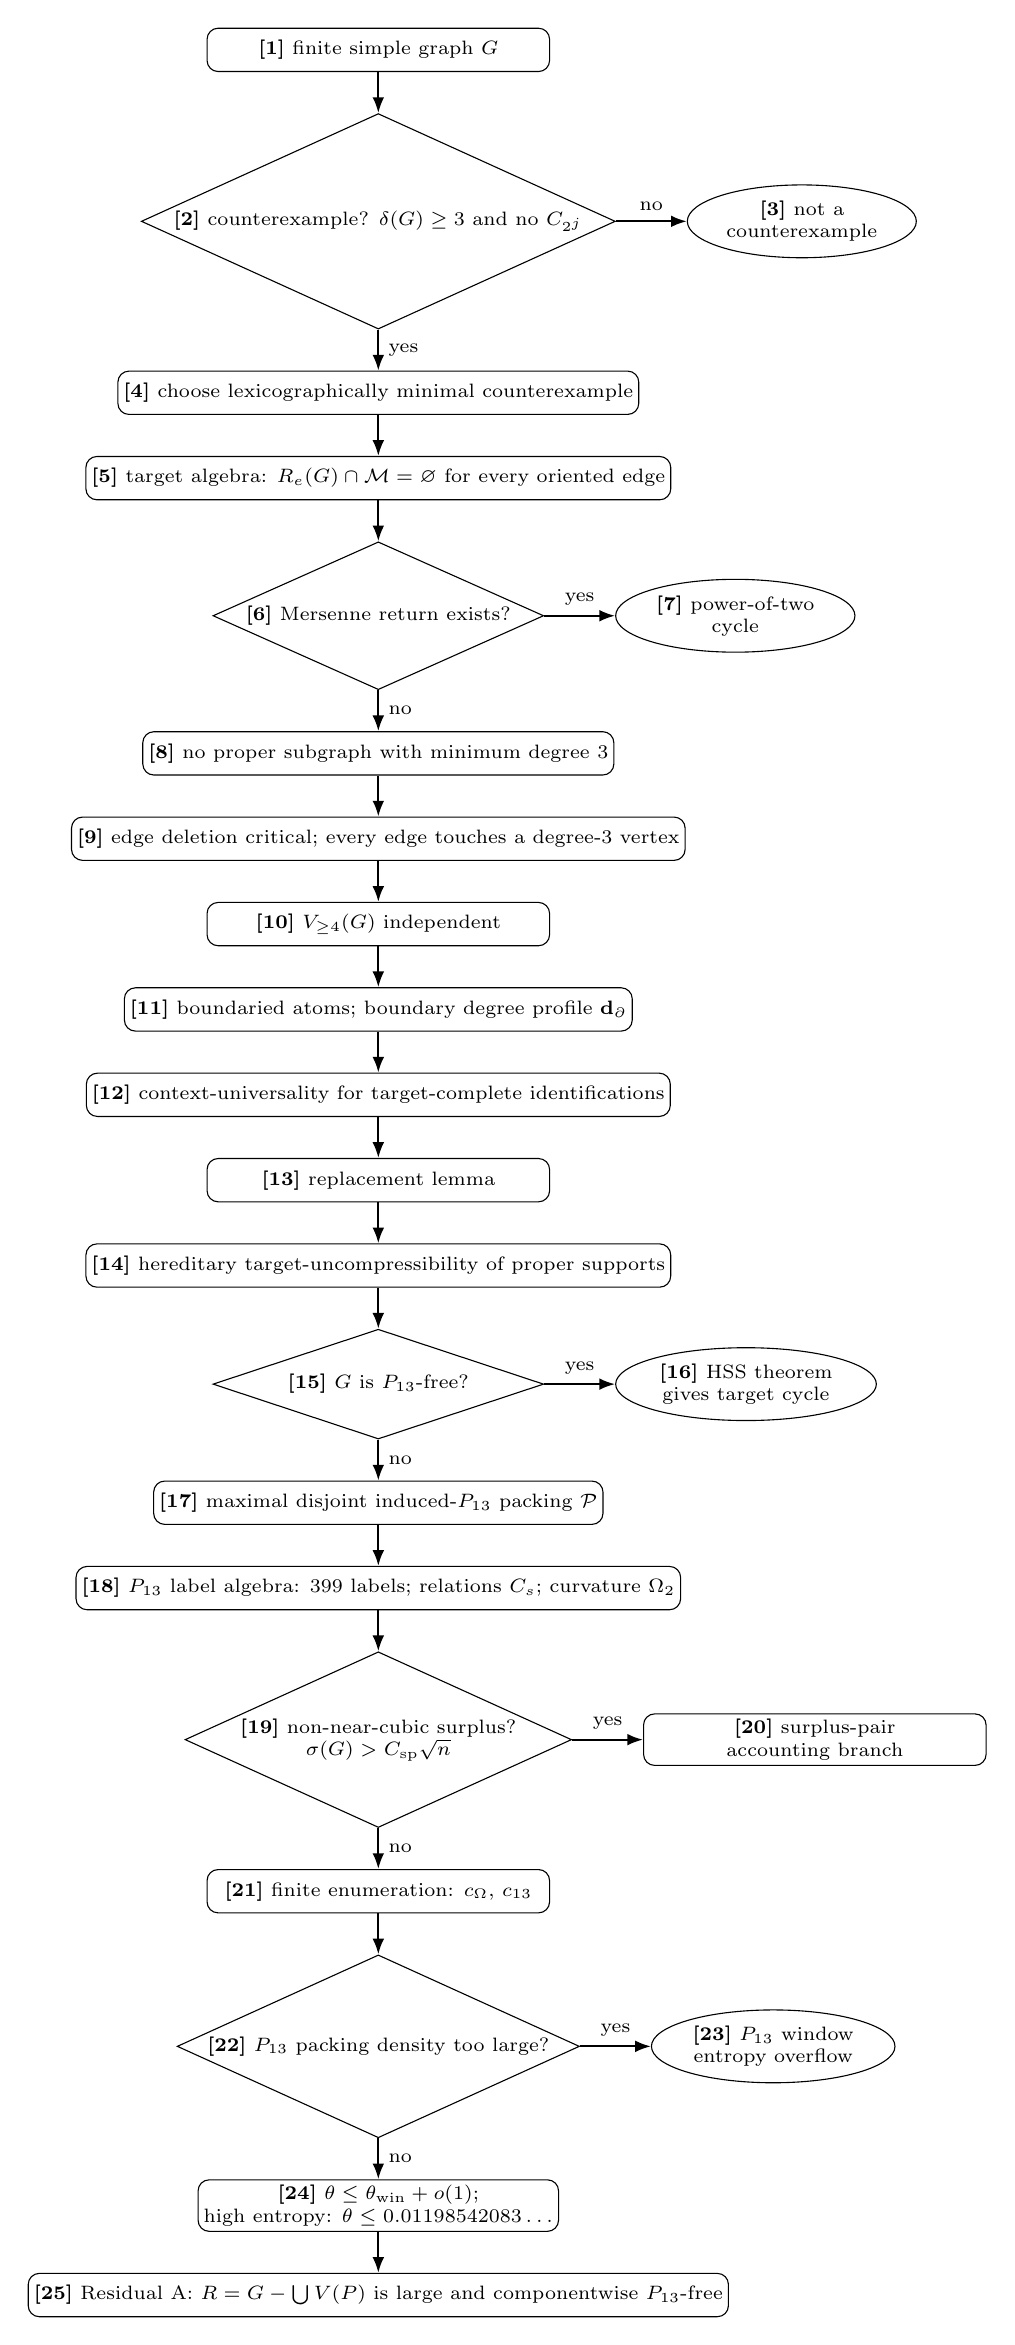
\begin{tikzpicture}[
node distance=0.52cm and 0.90cm,
box/.style={rectangle,rounded corners,draw,align=center,inner sep=2pt,minimum width=4.35cm,minimum height=0.55cm},
dec/.style={diamond,draw,aspect=2.2,align=center,inner sep=1pt,minimum width=4.2cm},
term/.style={ellipse,draw,align=center,inner sep=2pt,minimum width=2.75cm},
arrow/.style={-{Latex[length=2mm]},thick},
every node/.style={font=\scriptsize}
]
\node[box] (G) {\textbf{[1]}~finite simple graph $G$};
\node[dec, below=of G] (bad) {\textbf{[2]}~counterexample? $\delta(G)\ge3$ and no $C_{2^j}$};
\node[term, right=of bad] (notbad) {\textbf{[3]}~not a\\counterexample};
\node[box, below=of bad] (min) {\textbf{[4]}~choose lexicographically minimal counterexample};
\node[box, below=of min] (target) {\textbf{[5]}~target algebra: $R_e(G)\cap\Mers=\varnothing$ for every oriented edge};
\node[dec, below=of target] (ret) {\textbf{[6]}~Mersenne return exists?};
\node[term, right=of ret] (cycle) {\textbf{[7]}~power-of-two\\cycle};
\node[box, below=of ret] (core) {\textbf{[8]}~no proper subgraph with minimum degree $3$};
\node[box, below=of core] (delete) {\textbf{[9]}~edge deletion critical; every edge touches a degree-$3$ vertex};
\node[box, below=of delete] (hiind) {\textbf{[10]}~$V_{\ge4}(G)$ independent};
\node[box, below=of hiind] (bd) {\textbf{[11]}~boundaried atoms; boundary degree profile $\mathbf d_\partial$};
\node[box, below=of bd] (univ) {\textbf{[12]}~context-universality for target-complete identifications};
\node[box, below=of univ] (replace) {\textbf{[13]}~replacement lemma};
\node[box, below=of replace] (uncomp) {\textbf{[14]}~hereditary target-uncompressibility of proper supports};
\node[dec, below=of uncomp] (p13free) {\textbf{[15]}~$G$ is $P_{13}$-free?};
\node[term, right=of p13free] (hss) {\textbf{[16]}~HSS theorem\\gives target cycle};
\node[box, below=of p13free] (pack) {\textbf{[17]}~maximal disjoint induced-$P_{13}$ packing $\mathcal P$};
\node[box, below=of pack] (p13alg) {\textbf{[18]}~$P_{13}$ label algebra: $399$ labels; relations $C_s$; curvature $\Omega_2$};
\node[dec, below=of p13alg] (surplusq) {\textbf{[19]}~non-near-cubic surplus?\\$\sigma(G)>C_{\rm sp}\sqrt n$};
\node[box, right=of surplusq] (surplusclose) {\textbf{[20]}~surplus-pair\\accounting branch};
\node[box, below=of surplusq] (enum) {\textbf{[21]}~finite enumeration: $c_\Omega$, $c_{13}$};
\node[dec, below=of enum] (many) {\textbf{[22]}~$P_{13}$ packing density too large?};
\node[term, right=of many] (overflow) {\textbf{[23]}~$P_{13}$ window\\entropy overflow};
\node[box, below=of many] (theta) {\textbf{[24]}~$\theta\le\theta_{\rm win}+o(1)$;\\high entropy: $\theta\le0.01198542083\ldots$};
\node[box, below=of theta] (R) {\textbf{[25]}~Residual A: $R=G-\bigcup V(P)$ is large and componentwise $P_{13}$-free};
\draw[arrow] (G)--(bad);
\draw[arrow] (bad)--node[above]{no}(notbad);
\draw[arrow] (bad)--node[right]{yes}(min);
\draw[arrow] (min)--(target);
\draw[arrow] (target)--(ret);
\draw[arrow] (ret)--node[above]{yes}(cycle);
\draw[arrow] (ret)--node[right]{no}(core);
\draw[arrow] (core)--(delete);
\draw[arrow] (delete)--(hiind);
\draw[arrow] (hiind)--(bd);
\draw[arrow] (bd)--(univ);
\draw[arrow] (univ)--(replace);
\draw[arrow] (replace)--(uncomp);
\draw[arrow] (uncomp)--(p13free);
\draw[arrow] (p13free)--node[above]{yes}(hss);
\draw[arrow] (p13free)--node[right]{no}(pack);
\draw[arrow] (pack)--(p13alg);
\draw[arrow] (p13alg)--(surplusq);
\draw[arrow] (surplusq)--node[above]{yes}(surplusclose);
\draw[arrow] (surplusq)--node[right]{no}(enum);
\draw[arrow] (enum)--(many);
\draw[arrow] (many)--node[above]{yes}(overflow);
\draw[arrow] (many)--node[right]{no}(theta);
\draw[arrow] (theta)--(R);
\end{tikzpicture}%
}
\caption[Proof-dependency diagram, Part I]{Proof-dependency diagram, Part I.  Rectangles are assertions or residual states, diamonds are yes/no branch tests, ellipses are terminal outcomes, and edge labels such as yes or no state which branch is followed.  The bracketed numbers are unique diagram-node numbers used by the dependency table.  Nodes [19] and [20] record the non-near-cubic surplus accounting branch used before the normalized spine budget; node [20] is the continuation expanded in \cref{fig:proof-diagram-part-x}, and node [25] continues in \cref{fig:proof-diagram-part-ii}.}
\label{fig:proof-diagram-part-i}
\end{figure}

\clearpage
\begin{figure}[p]
\centering
\resizebox{0.96\textwidth}{0.82\textheight}{%
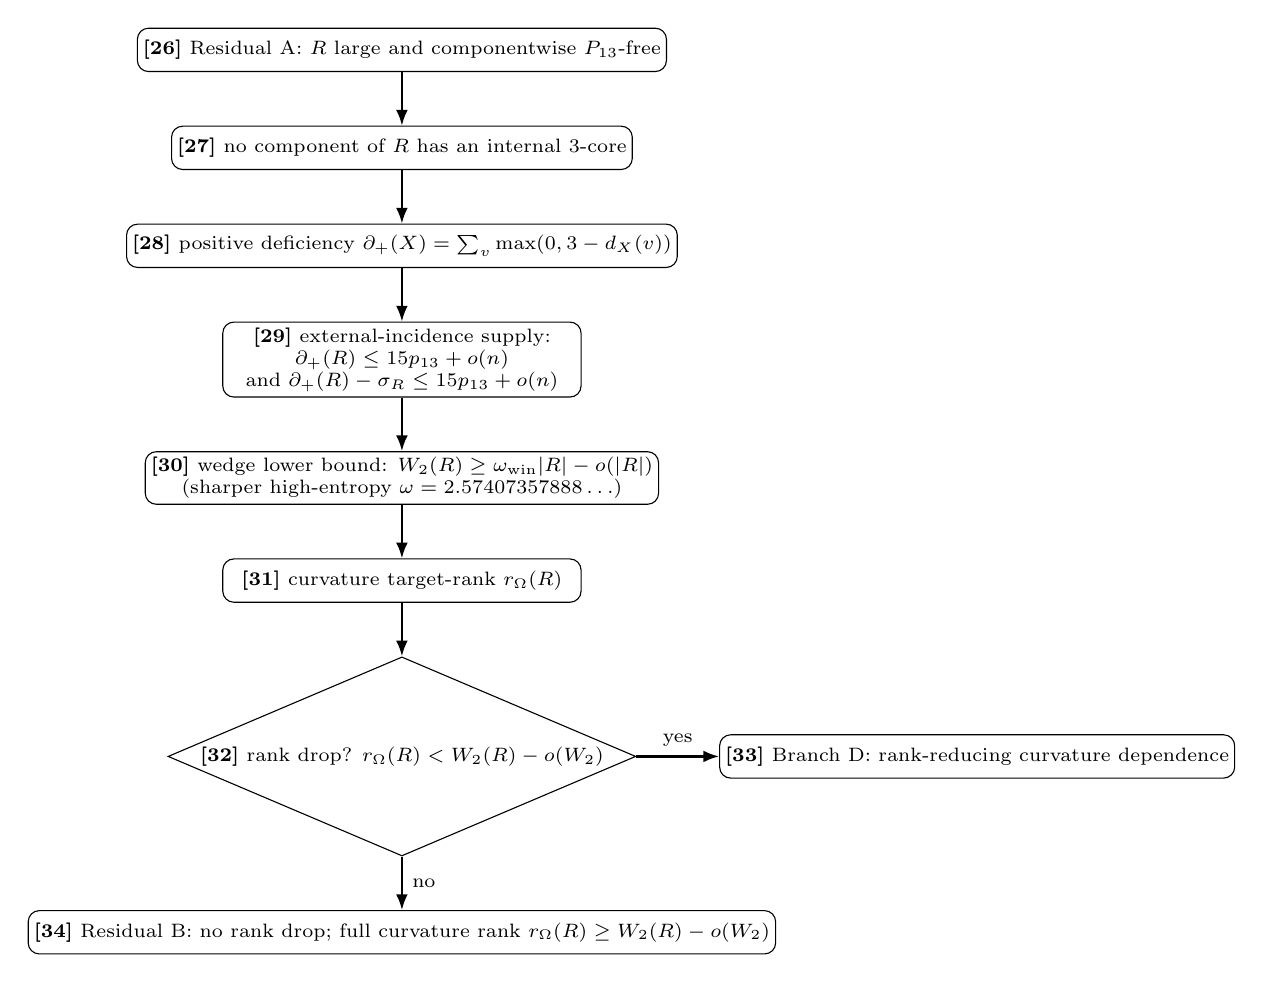
\begin{tikzpicture}[
node distance=0.68cm and 1.05cm,
box/.style={rectangle,rounded corners,draw,align=center,inner sep=2pt,minimum width=4.55cm,minimum height=0.55cm},
dec/.style={diamond,draw,aspect=2.35,align=center,inner sep=1pt,minimum width=4.35cm},
term/.style={ellipse,draw,align=center,inner sep=2pt,minimum width=3.1cm},
arrow/.style={-{Latex[length=2mm]},thick},
every node/.style={font=\scriptsize}
]
\node[box] (R) {\textbf{[26]}~Residual A: $R$ large and componentwise $P_{13}$-free};
\node[box, below=of R] (no3) {\textbf{[27]}~no component of $R$ has an internal $3$-core};
\node[box, below=of no3] (defp) {\textbf{[28]}~positive deficiency $\defp(X)=\sum_v\max(0,3-d_X(v))$};
\node[box, below=of defp] (stub) {\textbf{[29]}~external-incidence supply:\\$\defp(R)\le15p_{13}+o(n)$\\and $\defp(R)-\sigma_R\le15p_{13}+o(n)$};
\node[box, below=of stub] (wedge) {\textbf{[30]}~wedge lower bound: $W_2(R)\ge\omega_{\rm win}|R|-o(|R|)$\\(sharper high-entropy $\omega=2.57407357888\ldots$)};
\node[box, below=of wedge] (rank) {\textbf{[31]}~curvature target-rank $r_\Omega(R)$};
\node[dec, below=of rank] (drop) {\textbf{[32]}~rank drop? $r_\Omega(R)<W_2(R)-o(W_2)$};
\node[box, right=of drop] (depopen) {\textbf{[33]}~Branch D: rank-reducing curvature dependence};
\node[box, below=of drop] (fullrank) {\textbf{[34]}~Residual B: no rank drop; full curvature rank $r_\Omega(R)\ge W_2(R)-o(W_2)$};
\draw[arrow] (R)--(no3);
\draw[arrow] (no3)--(defp);
\draw[arrow] (defp)--(stub);
\draw[arrow] (stub)--(wedge);
\draw[arrow] (wedge)--(rank);
\draw[arrow] (rank)--(drop);
\draw[arrow] (drop)--node[above]{yes}(depopen);
\draw[arrow] (drop)--node[right]{no}(fullrank);
\end{tikzpicture}%
}
\caption[Proof-dependency diagram, Part II]{Proof-dependency diagram, Part II.  Rectangles, diamonds, ellipses, bracketed node numbers, and edge labels use the convention of \cref{fig:proof-diagram-part-i}.  At node [29], \(\sigma_R=\sigma(R)\) denotes the ambient surplus on the remainder; the positive-deficiency bound \(\defp(R)\le15p_{13}+o(n)\) is the incidence-supply input, and the \(\defp(R)-\sigma_R\) bound is its surplus-adjusted consequence.  The diagram produces two continuations: the rank-drop branch, closed in Part III, and the full-rank residual, continued in Part IV.}
\label{fig:proof-diagram-part-ii}
\end{figure}

\clearpage
\begin{figure}[p]
\centering
\resizebox{0.96\textwidth}{0.82\textheight}{%
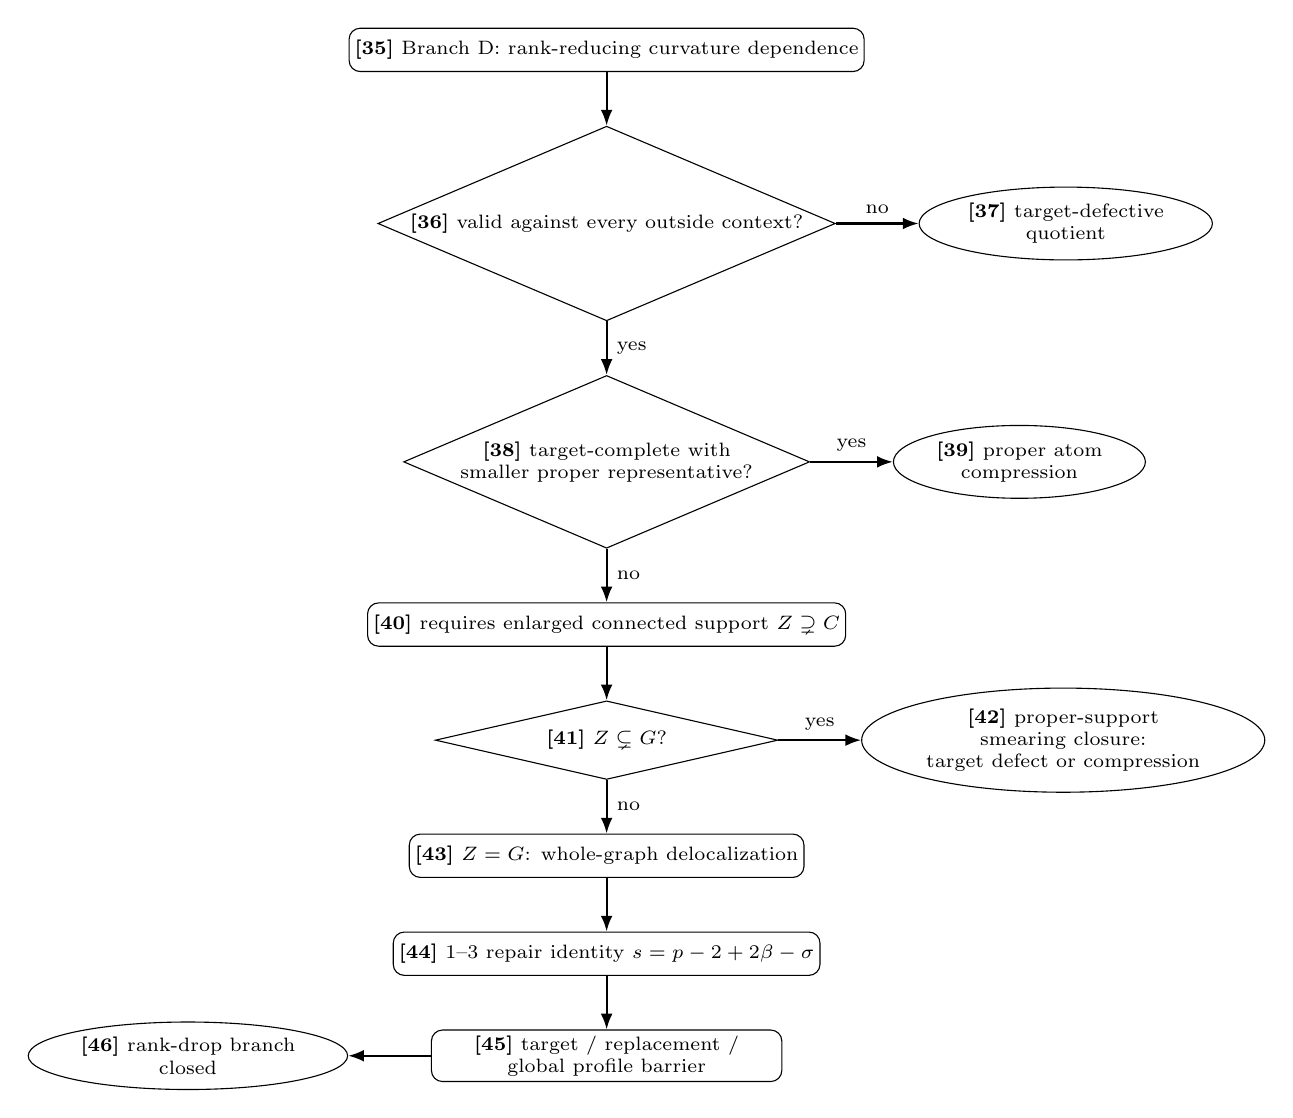
\begin{tikzpicture}[
node distance=0.68cm and 1.05cm,
box/.style={rectangle,rounded corners,draw,align=center,inner sep=2pt,minimum width=4.45cm,minimum height=0.55cm},
dec/.style={diamond,draw,aspect=2.35,align=center,inner sep=1pt,minimum width=4.35cm},
term/.style={ellipse,draw,align=center,inner sep=2pt,minimum width=3.2cm},
arrow/.style={-{Latex[length=2mm]},thick},
every node/.style={font=\scriptsize}
]
\node[box] (dep) {\textbf{[35]}~Branch D: rank-reducing curvature dependence};
\node[dec, below=of dep] (ctx) {\textbf{[36]}~valid against every outside context?};
\node[term, right=of ctx] (defect) {\textbf{[37]}~target-defective\\quotient};
\node[dec, below=of ctx] (atom) {\textbf{[38]}~target-complete with\\smaller proper representative?};
\node[term, right=of atom] (atomterm) {\textbf{[39]}~proper atom\\compression};
\node[box, below=of atom] (Z) {\textbf{[40]}~requires enlarged connected support $Z\supsetneq C$};
\node[dec, below=of Z] (properZ) {\textbf{[41]}~$Z\subsetneq G$?};
\node[term, right=of properZ] (properterm) {\textbf{[42]}~proper-support\\smearing closure:\\target defect or compression};
\node[box, below=of properZ] (global) {\textbf{[43]}~$Z=G$: whole-graph delocalization};
\node[box, below=of global] (rankwall) {\textbf{[44]}~$1$--$3$ repair identity $s=p-2+2\beta-\sigma$};
\node[box, below=of rankwall] (globalterm) {\textbf{[45]}~target / replacement /\\global profile barrier};
\node[term, left=of globalterm] (closed) {\textbf{[46]}~rank-drop branch\\closed};
\draw[arrow] (dep)--(ctx);
\draw[arrow] (ctx)--node[above]{no}(defect);
\draw[arrow] (ctx)--node[right]{yes}(atom);
\draw[arrow] (atom)--node[above]{yes}(atomterm);
\draw[arrow] (atom)--node[right]{no}(Z);
\draw[arrow] (Z)--(properZ);
\draw[arrow] (properZ)--node[above]{yes}(properterm);
\draw[arrow] (properZ)--node[right]{no}(global);
\draw[arrow] (global)--(rankwall);
\draw[arrow] (rankwall)--(globalterm);
\draw[arrow] (globalterm)--(closed);
\end{tikzpicture}%
}
\caption[Proof-dependency diagram, Part III]{Proof-dependency diagram, Part III.  Rectangles, diamonds, ellipses, bracketed node numbers, and edge labels use the convention of \cref{fig:proof-diagram-part-i}.  Every rank-drop branch terminates in a closed round node.}
\label{fig:proof-diagram-part-iii}
\end{figure}

\clearpage
\begin{figure}[p]
\centering
\resizebox{0.96\textwidth}{0.82\textheight}{%
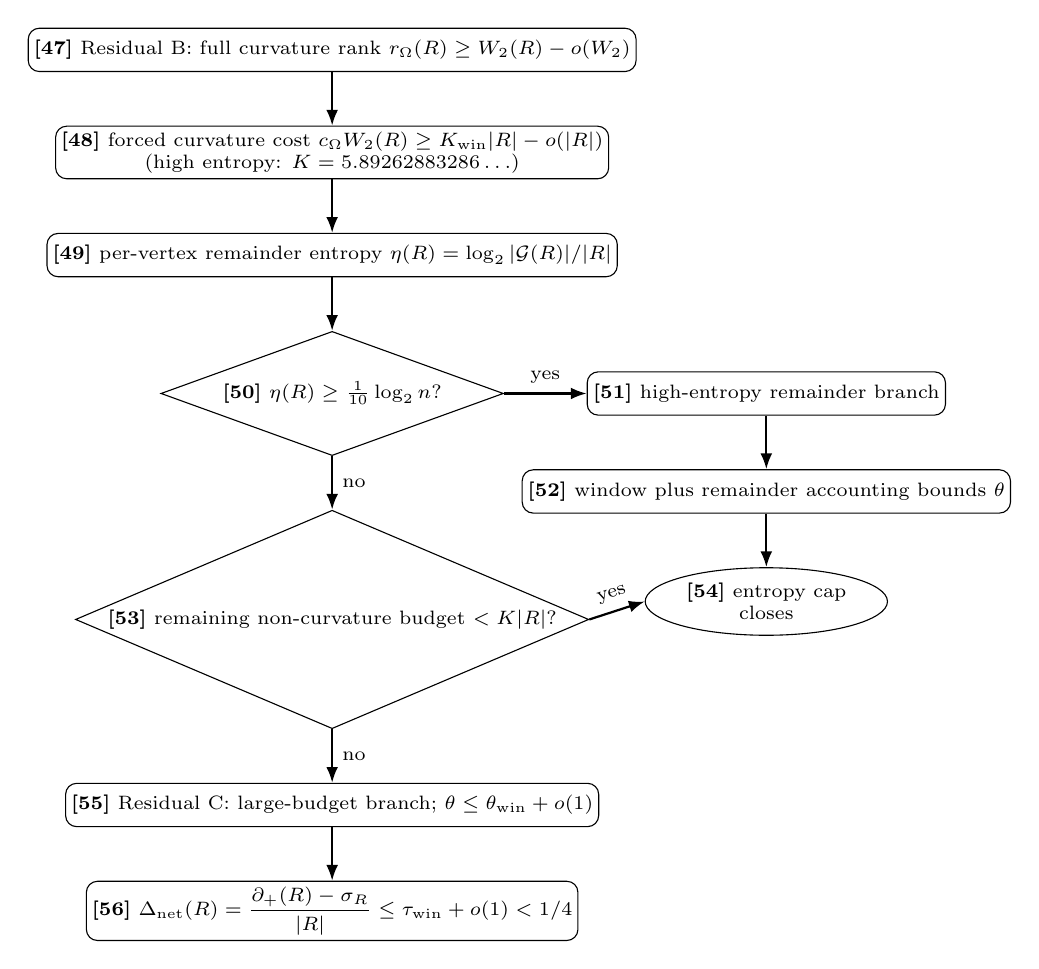
\begin{tikzpicture}[
node distance=0.68cm and 1.05cm,
box/.style={rectangle,rounded corners,draw,align=center,inner sep=2pt,minimum width=4.55cm,minimum height=0.55cm},
dec/.style={diamond,draw,aspect=2.35,align=center,inner sep=1pt,minimum width=4.35cm},
term/.style={ellipse,draw,align=center,inner sep=2pt,minimum width=3.0cm},
arrow/.style={-{Latex[length=2mm]},thick},
every node/.style={font=\scriptsize}
]
\node[box] (fullrank) {\textbf{[47]}~Residual B: full curvature rank $r_\Omega(R)\ge W_2(R)-o(W_2)$};
\node[box, below=of fullrank] (cost) {\textbf{[48]}~forced curvature cost $c_\Omega W_2(R)\ge K_{\rm win}|R|-o(|R|)$\\(high entropy: $K=5.89262883286\ldots$)};
\node[box, below=of cost] (eta) {\textbf{[49]}~per-vertex remainder entropy $\eta(R)=\log_2|\mathcal G(R)|/|R|$};
\node[dec, below=of eta] (expensive) {\textbf{[50]}~$\eta(R)\ge\frac1{10}\log_2 n$?};
\node[box, right=of expensive] (expbranch) {\textbf{[51]}~high-entropy remainder branch};
\node[box, below=of expbranch] (windowacct) {\textbf{[52]}~window plus remainder accounting bounds $\theta$};
\node[dec, below=of expensive] (smallbudget) {\textbf{[53]}~remaining non-curvature budget $<K|R|$?};
\node[term, below=of windowacct] (entcap) {\textbf{[54]}~entropy cap\\closes};
\node[box, below=of smallbudget] (thetaN) {\textbf{[55]}~Residual C: large-budget branch; $\theta\le\theta_{\rm win}+o(1)$};
\node[box, below=of thetaN] (netcap) {\textbf{[56]}~$\Delta_{\mathrm{net}}(R)=\dfrac{\defp(R)-\sigma_R}{|R|}\le\tau_{\rm win}+o(1)<1/4$};
\draw[arrow] (fullrank)--(cost);
\draw[arrow] (cost)--(eta);
\draw[arrow] (eta)--(expensive);
\draw[arrow] (expensive)--node[above]{yes}(expbranch);
\draw[arrow] (expbranch)--(windowacct);
\draw[arrow] (windowacct)--(entcap);
\draw[arrow] (expensive)--node[right]{no}(smallbudget);
\draw[arrow] (smallbudget.east)--node[above,sloped]{yes}(entcap.west);
\draw[arrow] (smallbudget)--node[right]{no}(thetaN);
\draw[arrow] (thetaN)--(netcap);
\end{tikzpicture}%
}
\caption[Proof-dependency diagram, Part IV]{Proof-dependency diagram, Part IV.  Rectangles, diamonds, ellipses, bracketed node numbers, and edge labels use the convention of \cref{fig:proof-diagram-part-i}.  The surviving continuation node is the large-budget net-deficiency residual.}
\label{fig:proof-diagram-part-iv}
\end{figure}

\clearpage

\begin{figure}[p]
\centering
\resizebox{0.98\textwidth}{!}{%
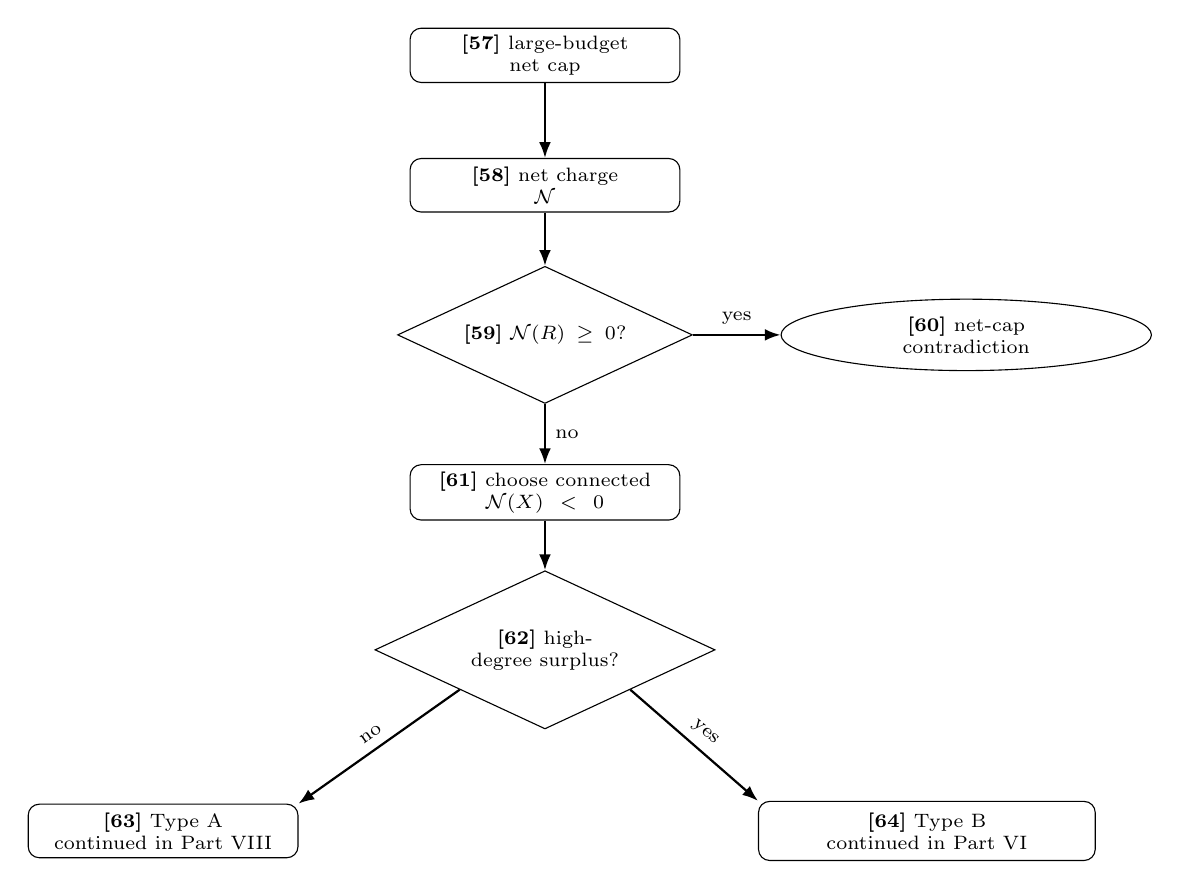
\begin{tikzpicture}[
box/.style={rectangle,rounded corners,draw,align=center,inner sep=2.5pt,text width=3.25cm,minimum height=0.68cm},
wide/.style={rectangle,rounded corners,draw,align=center,inner sep=2.5pt,text width=4.10cm,minimum height=0.75cm},
dec/.style={diamond,draw,aspect=2.15,align=center,inner sep=1.2pt,text width=2.95cm},
term/.style={ellipse,draw,align=center,inner sep=2.5pt,text width=3.15cm,minimum height=0.70cm},
arrow/.style={-{Latex[length=2mm]},thick},
every node/.style={font=\scriptsize}
]
\node[box] (netcap) at (0.00,6.90) {\textbf{[57]}~large-budget\\net cap};
\node[box] (Ndef) at (0.00,5.25) {\textbf{[58]}~net charge\\\(\No\)};
\node[dec] (globalnet) at (0.00,3.35) {\textbf{[59]}~\(\No(R)\ge0\)?};
\node[term] (contrad) at (5.35,3.35) {\textbf{[60]}~net-cap\\contradiction};
\node[box] (minX) at (0.00,1.35) {\textbf{[61]}~choose connected\\\(\No(X)<0\)};
\node[dec] (surplus) at (0.00,-0.65) {\textbf{[62]}~high-degree surplus?};
\node[box] (typeA) at (-4.85,-2.95) {\textbf{[63]}~Type A\\continued in Part VIII};
\node[wide] (typeB) at (4.85,-2.95) {\textbf{[64]}~Type B\\continued in Part VI};
\draw[arrow] (netcap)--(Ndef);
\draw[arrow] (Ndef)--(globalnet);
\draw[arrow] (globalnet.east)--node[above]{yes}(contrad.west);
\draw[arrow] (globalnet)--node[right]{no}(minX);
\draw[arrow] (minX)--(surplus);
\draw[arrow] (surplus.south west)--node[above,sloped]{no}(typeA.north east);
\draw[arrow] (surplus.south east)--node[above,sloped]{yes}(typeB.north west);
\end{tikzpicture}%
}
\caption[Proof-dependency diagram, Part V]{Proof-dependency diagram, Part V.  Conventions are as in \cref{fig:proof-diagram-part-i}.  This panel performs the net-charge split [57]--[64].  Node [63] continues in \cref{fig:proof-diagram-part-viii}, and node [64] continues in \cref{fig:proof-diagram-part-vi}.}
\label{fig:proof-diagram-part-v}
\end{figure}

\clearpage

\begin{figure}[p]
\centering
\resizebox{0.98\textwidth}{!}{%
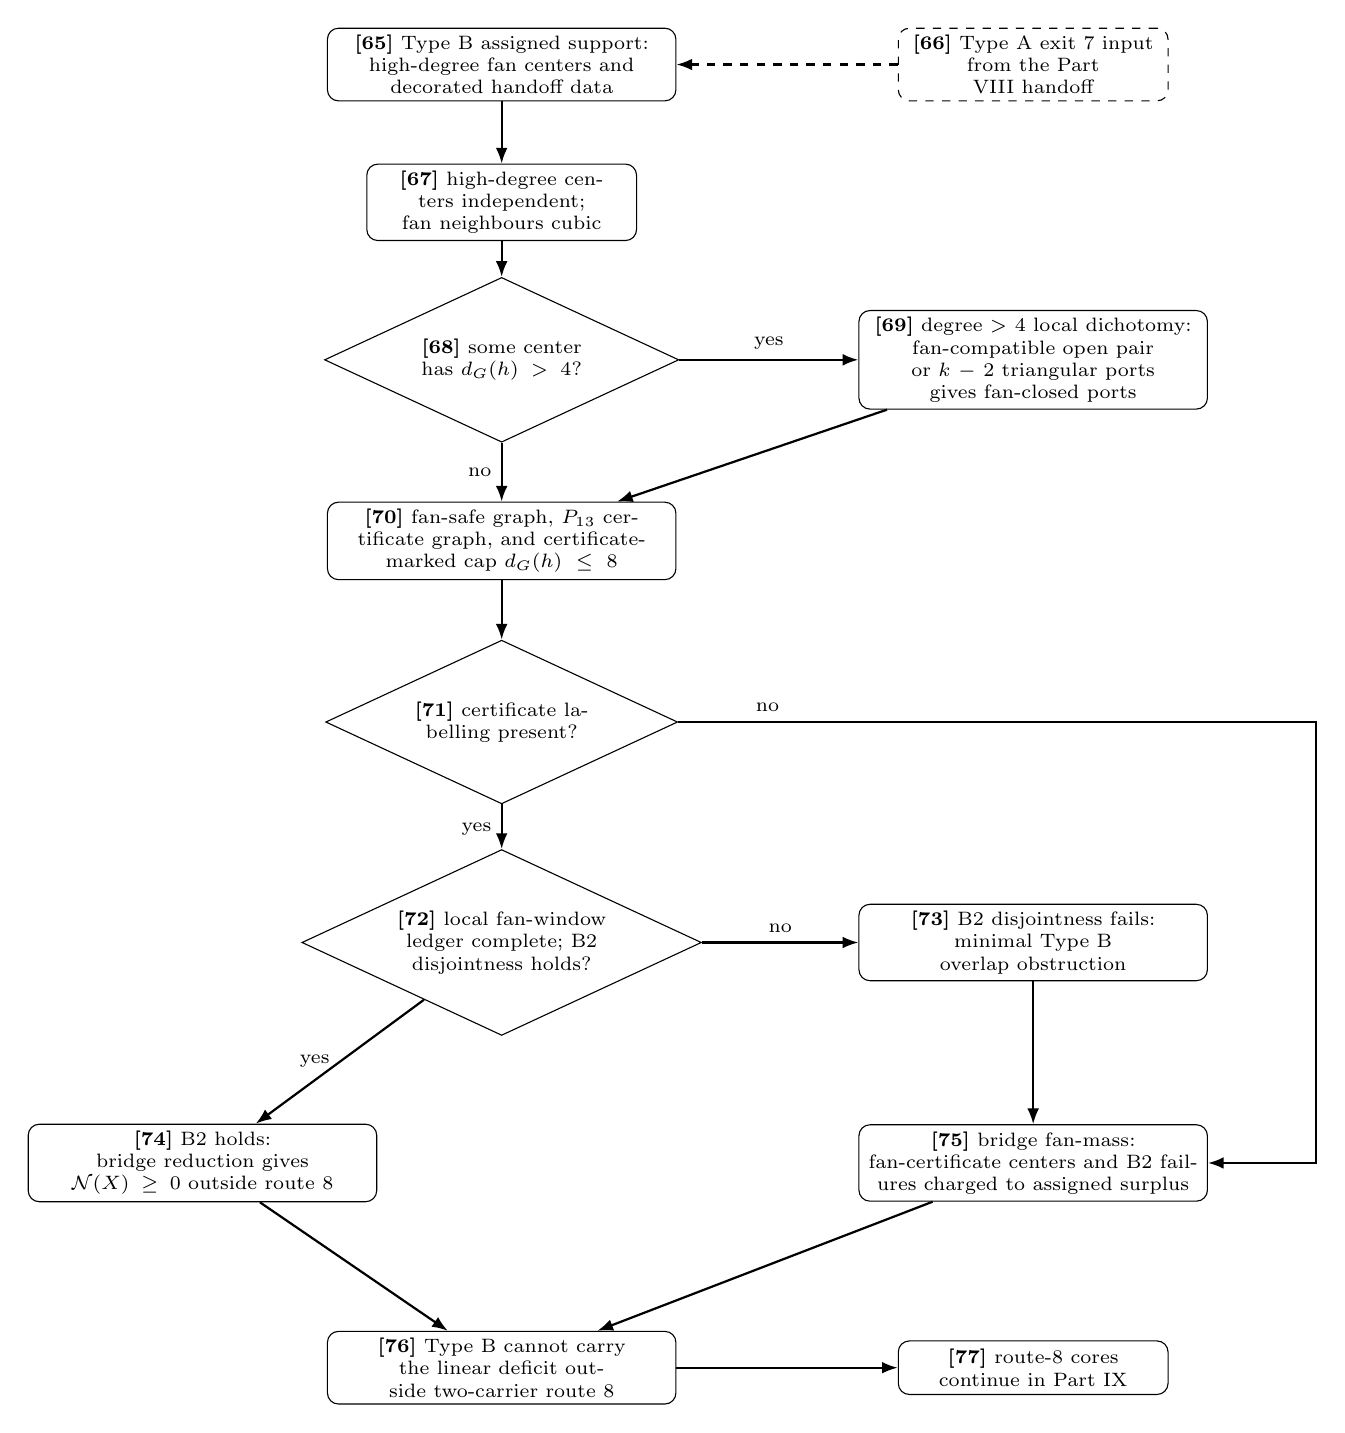
\begin{tikzpicture}[
box/.style={rectangle,rounded corners,draw,align=center,inner sep=2.5pt,text width=3.25cm,minimum height=0.68cm},
wide/.style={rectangle,rounded corners,draw,align=center,inner sep=2.5pt,text width=4.25cm,minimum height=0.78cm},
dec/.style={diamond,draw,aspect=2.15,align=center,inner sep=1.2pt,text width=3.10cm},
term/.style={ellipse,draw,align=center,inner sep=2.5pt,text width=3.15cm,minimum height=0.70cm},
arrow/.style={-{Latex[length=2mm]},thick},
every node/.style={font=\scriptsize}
]
\node[wide] (typeB) at (0.00,8.60) {\textbf{[65]}~Type B assigned support:\\high-degree fan centers and decorated handoff data};
\node[box,dashed] (decorB) at (6.75,8.60) {\textbf{[66]}~Type A exit 7 input\\from the Part VIII handoff};
\node[box] (highind) at (0.00,6.85) {\textbf{[67]}~high-degree centers independent; fan neighbours cubic};
\node[dec] (degsplit) at (0.00,4.85) {\textbf{[68]}~some center has \(d_G(h)>4\)?};
\node[wide] (localgt) at (6.75,4.85) {\textbf{[69]}~degree \(>4\) local dichotomy:\\fan-compatible open pair or \(k-2\) triangular ports gives fan-closed ports};
\node[wide] (fsafe) at (0.00,2.55) {\textbf{[70]}~fan-safe graph, \(P_{13}\) certificate graph, and certificate-marked cap \(d_G(h)\le8\)};
\node[dec] (certq) at (0.00,0.25) {\textbf{[71]}~certificate labelling present?};
\node[dec] (b2q) at (0.00,-2.55) {\textbf{[72]}~local fan-window ledger complete; B2 disjointness holds?};
\node[wide] (typeBres) at (6.75,-2.55) {\textbf{[73]}~B2 disjointness fails:\\minimal Type B overlap obstruction};
\node[wide] (fanthm) at (-3.80,-5.35) {\textbf{[74]}~B2 holds:\\bridge reduction gives \(\No(X)\ge0\) outside route 8};
\node[wide] (fanmass) at (6.75,-5.35) {\textbf{[75]}~bridge fan-mass:\\fan-certificate centers and B2 failures charged to assigned surplus};
\node[wide] (closed) at (0.00,-7.95) {\textbf{[76]}~Type B cannot carry the linear deficit outside two-carrier route 8};
\node[box] (route8) at (6.75,-7.95) {\textbf{[77]}~route-8 cores\\continue in Part IX};
\draw[arrow,dashed] (decorB.west)--(typeB.east);
\draw[arrow] (typeB)--(highind);
\draw[arrow] (highind)--(degsplit);
\draw[arrow] (degsplit)--node[above]{yes}(localgt);
\draw[arrow] (degsplit)--node[left]{no}(fsafe);
\draw[arrow] (localgt)--(fsafe);
\draw[arrow] (fsafe)--(certq);
\draw[arrow] (certq)--node[left,pos=.55]{yes}(b2q);
\draw[arrow] (certq.east)--node[above,pos=.14]{no}++(8.10,0)|-(fanmass.east);
\draw[arrow] (b2q)--node[above]{no}(typeBres);
\draw[arrow] (b2q)--node[left]{yes}(fanthm);
\draw[arrow] (typeBres)--(fanmass);
\draw[arrow] (fanthm)--(closed);
\draw[arrow] (fanmass)--(closed);
\draw[arrow] (closed)--(route8);
\end{tikzpicture}%
}
\caption[Proof-dependency diagram, Part VI]{Proof-dependency diagram, Part VI.  The Type B continuation starts from node [64], receives the incoming Type A handoff through the dashed input [66], splits at [68], and applies [69]--[76] before the route-8 continuation [77].  The degree-\(4\) no-branch of [68] is expanded in \cref{fig:proof-diagram-part-vii}.}
\label{fig:proof-diagram-part-vi}
\end{figure}

\clearpage

\begin{figure}[p]
\centering
\resizebox{0.98\textwidth}{!}{%
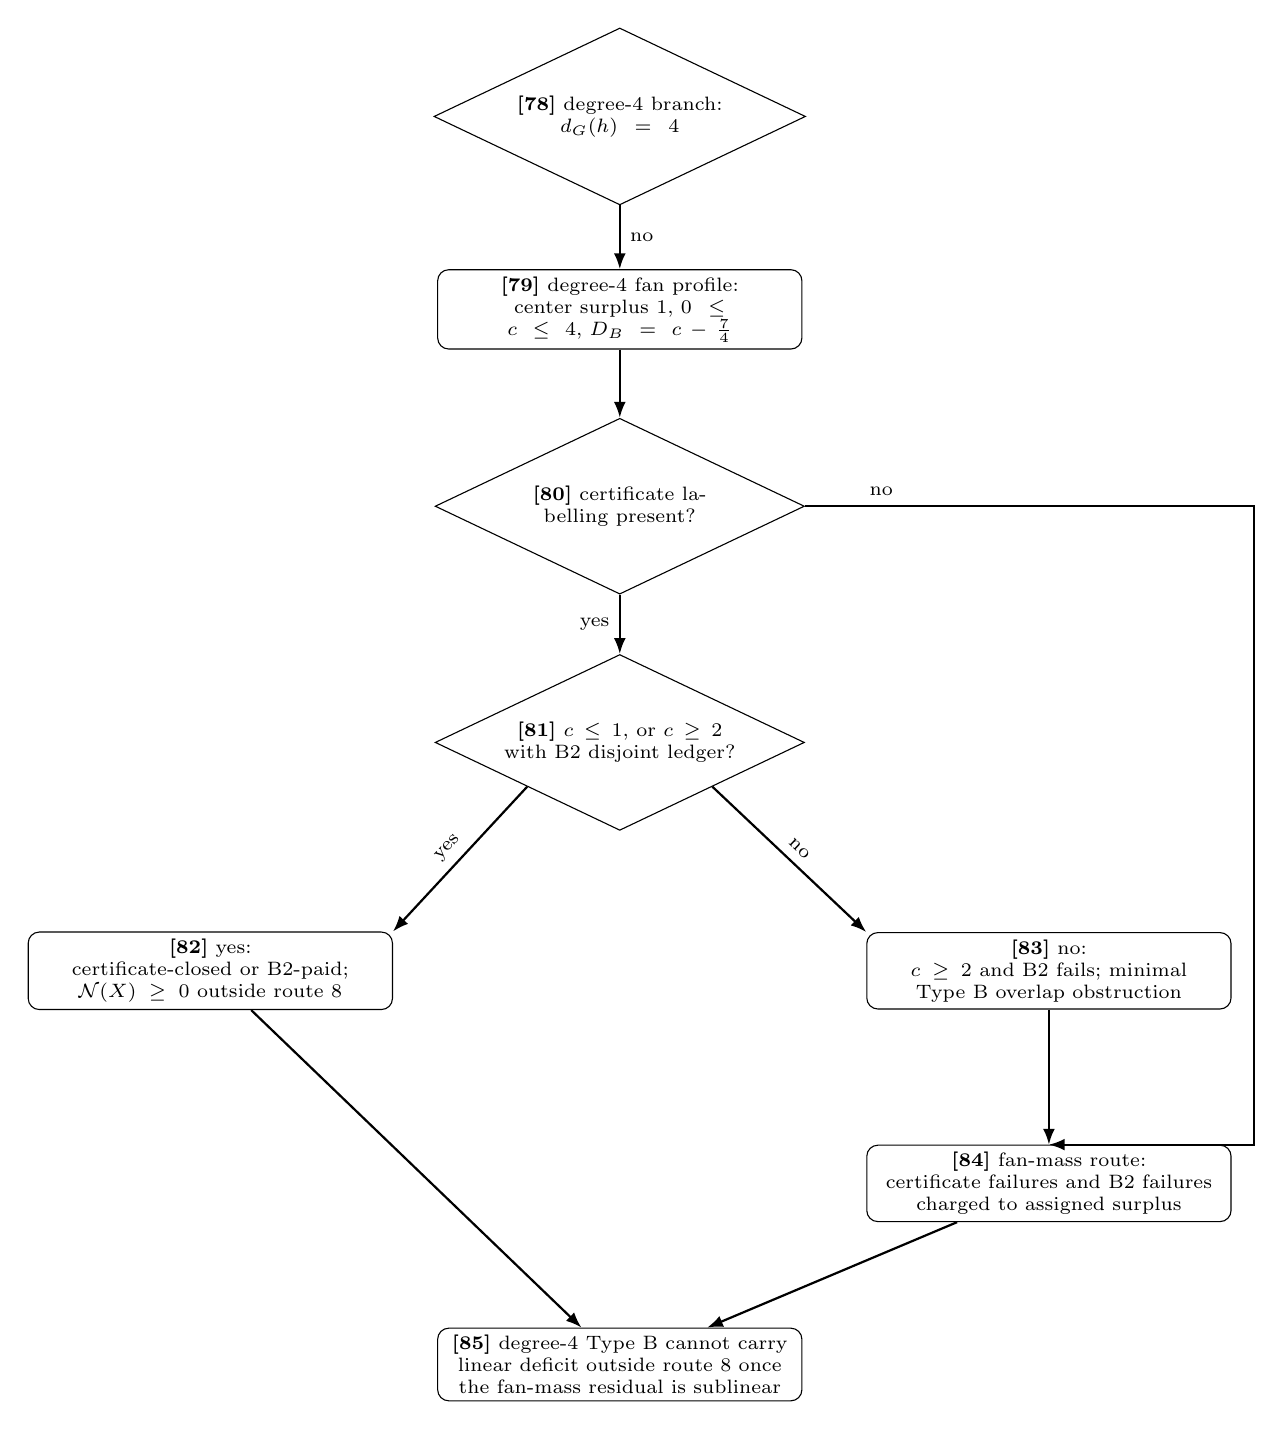
\begin{tikzpicture}[
box/.style={rectangle,rounded corners,draw,align=center,inner sep=2.5pt,text width=3.45cm,minimum height=0.72cm},
wide/.style={rectangle,rounded corners,draw,align=center,inner sep=2.5pt,text width=4.45cm,minimum height=0.82cm},
dec/.style={diamond,draw,aspect=2.10,align=center,inner sep=1.2pt,text width=3.35cm},
arrow/.style={-{Latex[length=2mm]},thick},
every node/.style={font=\scriptsize}
]
\node[dec] (split) at (0.00,6.60) {\textbf{[78]}~degree-\(4\) branch:\\\(d_G(h)=4\)};
\node[wide] (profile) at (0.00,4.15) {\textbf{[79]}~degree-\(4\) fan profile:\\center surplus \(1\), \(0\le c\le4\), \(D_B=c-\frac74\)};
\node[dec] (certq) at (0.00,1.65) {\textbf{[80]}~certificate labelling present?};
\node[dec] (ledgerq) at (0.00,-1.35) {\textbf{[81]}~\(c\le1\), or \(c\ge2\) with B2 disjoint ledger?};
\node[wide] (closedledger) at (-5.20,-4.25) {\textbf{[82]}~yes:\\certificate-closed or B2-paid; \(\No(X)\ge0\) outside route 8};
\node[wide] (overlap) at (5.45,-4.25) {\textbf{[83]}~no:\\\(c\ge2\) and B2 fails; minimal Type B overlap obstruction};
\node[wide] (fanmass) at (5.45,-6.95) {\textbf{[84]}~fan-mass route:\\certificate failures and B2 failures charged to assigned surplus};
\node[wide] (closed) at (0.00,-9.25) {\textbf{[85]}~degree-\(4\) Type B cannot carry linear deficit outside route 8 once the fan-mass residual is sublinear};
\draw[arrow] (split)--node[right]{no}(profile);
\draw[arrow] (profile)--(certq);
\draw[arrow] (certq)--node[left]{yes}(ledgerq);
\draw[arrow] (certq.east)--node[above,pos=.17]{no}++(5.70,0)|-(fanmass.north);
\draw[arrow] (ledgerq.south west)--node[above,sloped]{yes}(closedledger.north east);
\draw[arrow] (ledgerq.south east)--node[above,sloped]{no}(overlap.north west);
\draw[arrow] (overlap)--(fanmass);
\draw[arrow] (closedledger)--(closed);
\draw[arrow] (fanmass)--(closed);
\end{tikzpicture}%
}
\caption[Proof-dependency diagram, Part VII]{Proof-dependency diagram, Part VII.  This panel expands the degree-\(4\) no-branch of [68].  The local closed cases are \(c\le1\); the difficult degree-\(4\) cases are \(c=2,3,4\), where closure depends on the B1 incidence payment and the B2 disjoint ledger at [81], or else routes to the residual fan-mass node [84].}
\label{fig:proof-diagram-part-vii}
\end{figure}

\clearpage

\begin{figure}[p]
\centering
\resizebox{!}{0.735\textheight}{%
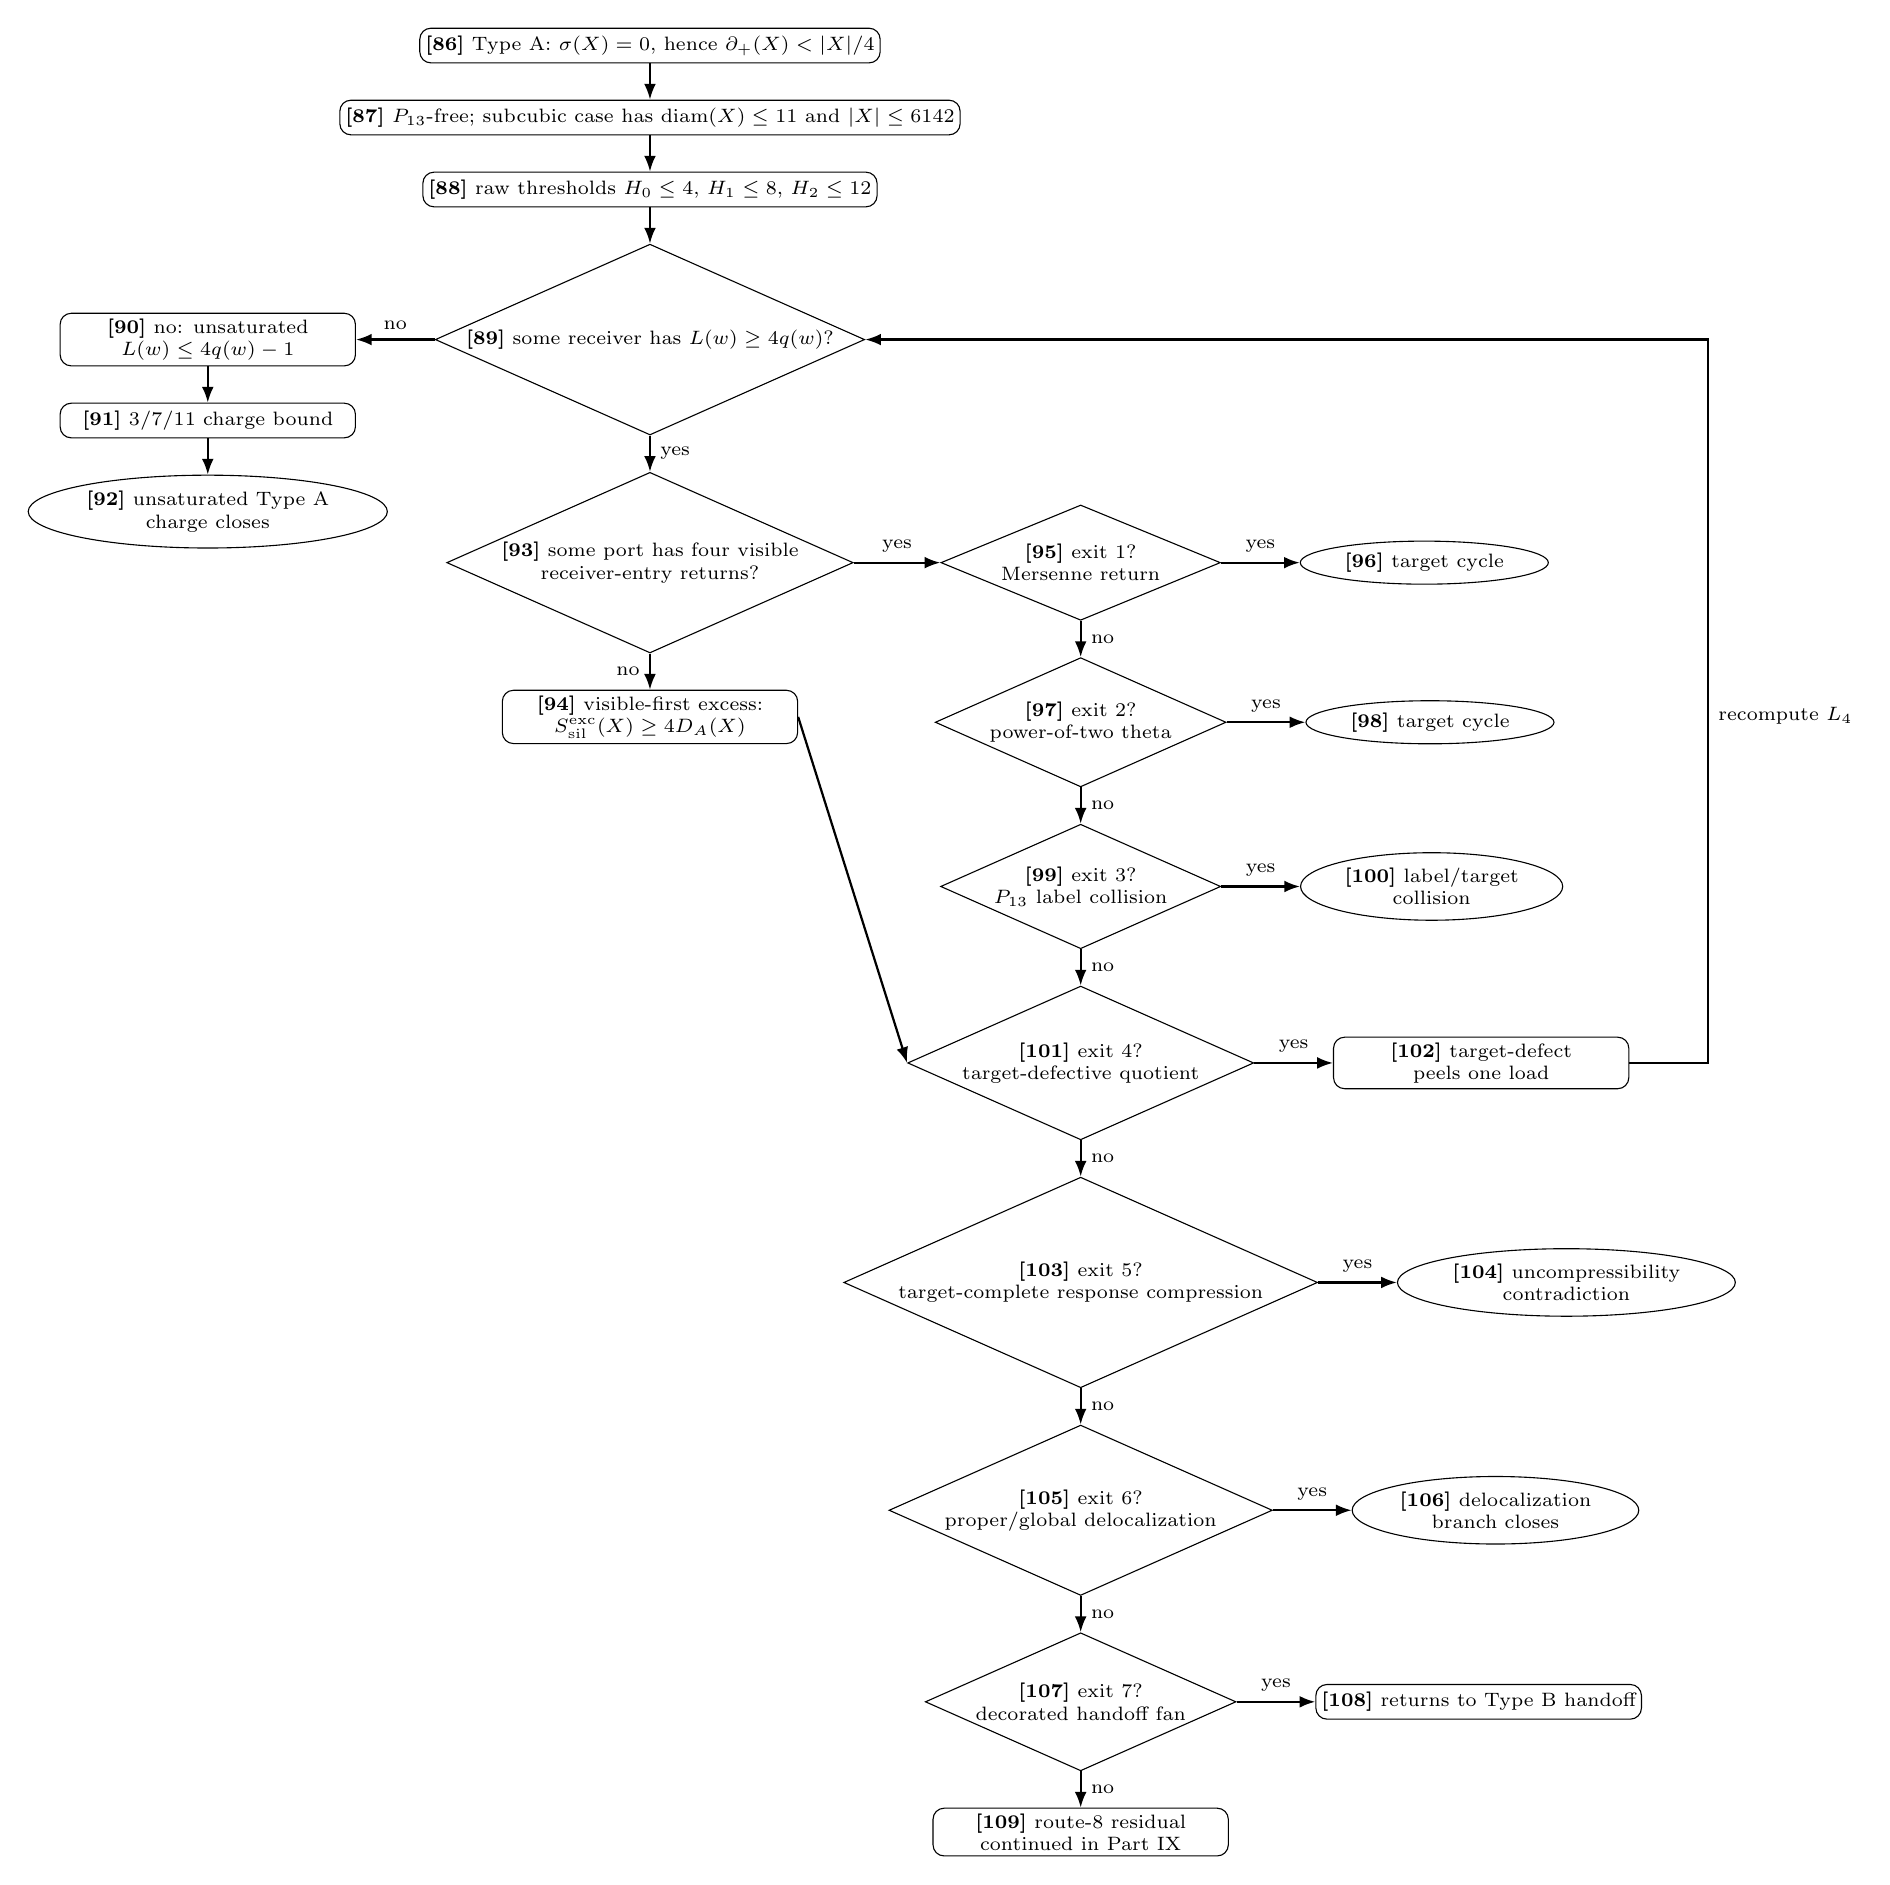
\begin{tikzpicture}[
node distance=0.46cm and 0.90cm,
box/.style={rectangle,rounded corners,draw,align=center,inner sep=2pt,minimum width=3.75cm,minimum height=0.44cm},
dec/.style={diamond,draw,aspect=2.25,align=center,inner sep=1pt,minimum width=3.55cm},
term/.style={ellipse,draw,align=center,inner sep=2pt,minimum width=3.15cm},
arrow/.style={-{Latex[length=2mm]},thick},
every node/.style={font=\scriptsize}
]
\node[box] (typeA) {\textbf{[86]}~Type A: $\sigma(X)=0$, hence $\defp(X)<|X|/4$};
\node[box, below=of typeA] (bounded) {\textbf{[87]}~$P_{13}$-free; subcubic case has $\diam(X)\le11$ and $|X|\le6142$};
\node[box, below=of bounded] (thresholds) {\textbf{[88]}~raw thresholds $H_0\le4$, $H_1\le8$, $H_2\le12$};
\node[dec, below=of thresholds] (saturated) {\textbf{[89]}~some receiver has $L(w)\ge4q(w)$?};
\node[box, left=1.00cm of saturated] (unsat) {\textbf{[90]}~no: unsaturated\\$L(w)\le4q(w)-1$};
\node[box, below=of unsat] (atomthm) {\textbf{[91]}~$3/7/11$ charge bound};
\node[term, below=of atomthm] (closed) {\textbf{[92]}~unsaturated Type A\\charge closes};
\node[dec, below=of saturated] (visq) {\textbf{[93]}~some port has four visible\\receiver-entry returns?};
\node[box, below=of visq] (silent) {\textbf{[94]}~visible-first excess:\\$S_{\rm sil}^{\rm exc}(X)\ge4D_A(X)$};
\node[dec, right=1.10cm of visq] (e1) {\textbf{[95]}~exit 1?\\Mersenne return};
\node[term, right=1.00cm of e1] (t1) {\textbf{[96]}~target cycle};
\node[dec, below=of e1] (e2) {\textbf{[97]}~exit 2?\\power-of-two theta};
\node[term, right=1.00cm of e2] (t2) {\textbf{[98]}~target cycle};
\node[dec, below=of e2] (e3) {\textbf{[99]}~exit 3?\\$P_{13}$ label collision};
\node[term, right=1.00cm of e3] (t3) {\textbf{[100]}~label/target\\collision};
\node[dec, below=of e3] (e4) {\textbf{[101]}~exit 4?\\target-defective quotient};
\node[box, right=1.00cm of e4] (t4) {\textbf{[102]}~target-defect\\peels one load};
\node[dec, below=of e4] (e5) {\textbf{[103]}~exit 5?\\target-complete response compression};
\node[term, right=1.00cm of e5] (t5) {\textbf{[104]}~uncompressibility\\contradiction};
\node[dec, below=of e5] (e6) {\textbf{[105]}~exit 6?\\proper/global delocalization};
\node[term, right=1.00cm of e6] (t6) {\textbf{[106]}~delocalization\\branch closes};
\node[dec, below=of e6] (e7) {\textbf{[107]}~exit 7?\\decorated handoff fan};
\node[box, right=1.00cm of e7] (decorB) {\textbf{[108]}~returns to Type B handoff};
\node[box, below=of e7] (route8) {\textbf{[109]}~route-8 residual\\continued in Part IX};
\draw[arrow] (typeA)--(bounded);
\draw[arrow] (bounded)--(thresholds);
\draw[arrow] (thresholds)--(saturated);
\draw[arrow] (saturated)--node[above]{no}(unsat);
\draw[arrow] (unsat)--(atomthm);
\draw[arrow] (atomthm)--(closed);
\draw[arrow] (saturated)--node[right]{yes}(visq);
\draw[arrow] (visq)--node[above]{yes}(e1);
\draw[arrow] (visq)--node[left]{no}(silent);
\draw[arrow] (silent.east) -- (e4.west);
\draw[arrow] (e1)--node[above]{yes}(t1);
\draw[arrow] (e1)--node[right]{no}(e2);
\draw[arrow] (e2)--node[above]{yes}(t2);
\draw[arrow] (e2)--node[right]{no}(e3);
\draw[arrow] (e3)--node[above]{yes}(t3);
\draw[arrow] (e3)--node[right]{no}(e4);
\draw[arrow] (e4)--node[above]{yes}(t4);
\draw[arrow] (t4.east) -- ++(1.00,0) |- node[pos=.24,right]{recompute \(L_4\)} (saturated.east);
\draw[arrow] (e4)--node[right]{no}(e5);
\draw[arrow] (e5)--node[above]{yes}(t5);
\draw[arrow] (e5)--node[right]{no}(e6);
\draw[arrow] (e6)--node[above]{yes}(t6);
\draw[arrow] (e6)--node[right]{no}(e7);
\draw[arrow] (e7)--node[above]{yes}(decorB);
\draw[arrow] (e7)--node[right]{no}(route8);
\end{tikzpicture}%
}
\caption[Proof-dependency diagram, Part VIII]{Proof-dependency diagram, Part VIII.  Rectangles, diamonds, ellipses, bracketed node numbers, and edge labels use the convention of \cref{fig:proof-diagram-part-i}.  Type A expands from node [63].  The $3/7/11$ calculation applies only after the saturated branch [89] has been exhausted.  If [89] is yes, exits 1--7 are tested explicitly: exits 1--3, 5, and 6 close at [96], [98], [100], [104], and [106], exit 4 peels one target-defective routed load at [102] and returns to [89] with the residual load \(L_4\), while exit 7 hands off to Type B [65] through node [108].  On the no-branch of [93], the visible-first excess calculation gives $S_{\rm sil}^{\rm exc}(X)\ge4D_A(X)$.  Exit (8), the route-8 residual [109], is expanded in \cref{fig:proof-diagram-part-ix}.}
\label{fig:proof-diagram-part-viii}
\end{figure}

\clearpage

\begin{figure}[p]
\centering
\resizebox{0.98\textwidth}{!}{%
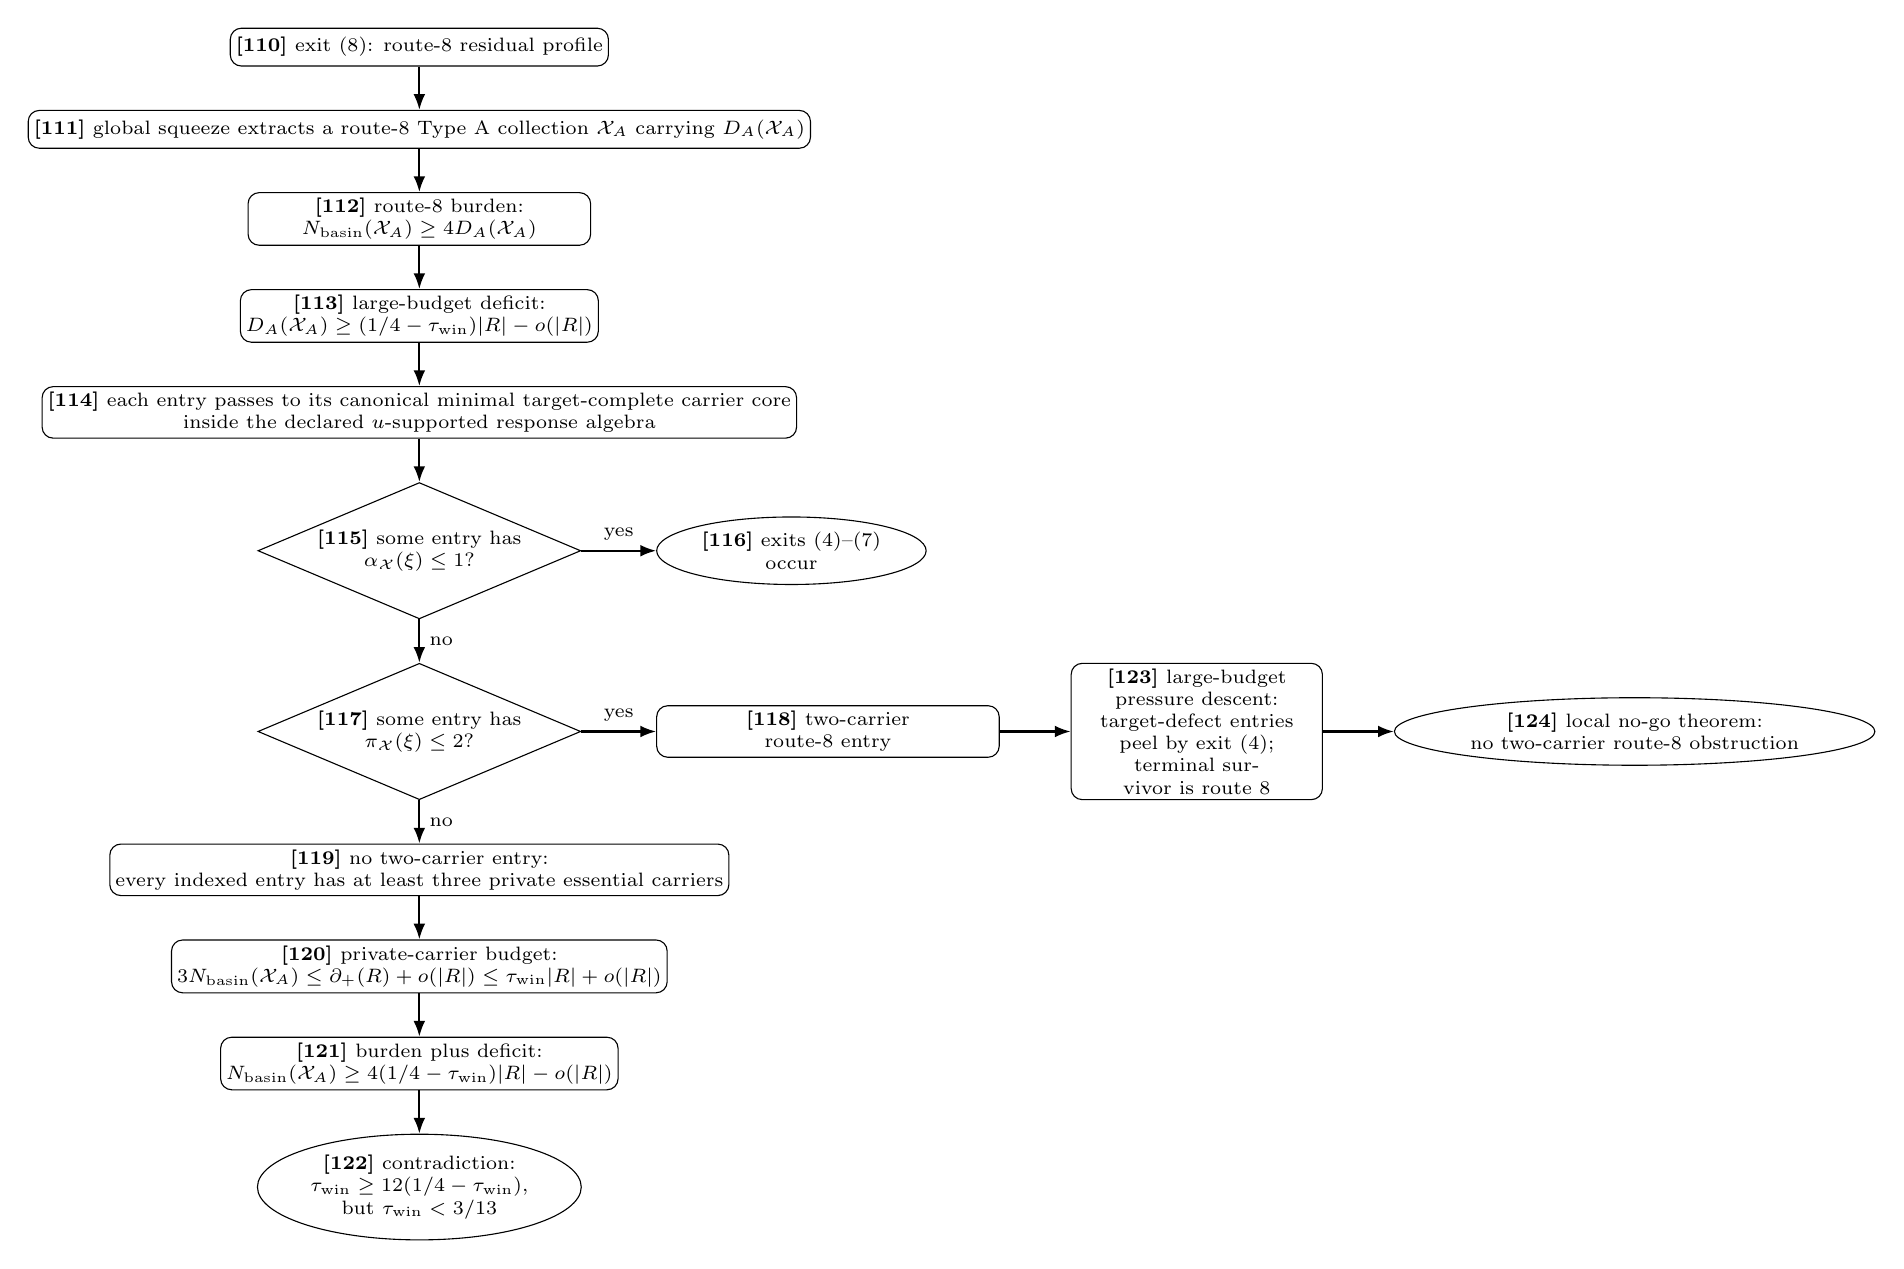
\begin{tikzpicture}[
node distance=0.55cm and 0.95cm,
box/.style={rectangle,rounded corners,draw,align=center,inner sep=2pt,minimum width=4.35cm,minimum height=0.48cm},
nobox/.style={rectangle,rounded corners,draw,align=center,inner sep=2pt,text width=3.05cm,minimum height=0.48cm},
dec/.style={diamond,draw,aspect=2.35,align=center,inner sep=1pt,minimum width=4.10cm},
term/.style={ellipse,draw,align=center,inner sep=2pt,minimum width=3.15cm},
arrow/.style={-{Latex[length=2mm]},thick},
every node/.style={font=\scriptsize}
]
\node[box] (route8) {\textbf{[110]}~exit (8): route-8 residual profile};
\node[box, below=of route8] (extract) {\textbf{[111]}~global squeeze extracts a route-8 Type A collection $\mathcal X_A$ carrying $D_A(\mathcal X_A)$};
\node[box, below=of extract] (burden) {\textbf{[112]}~route-8 burden:\\$N_{\rm basin}(\mathcal X_A)\ge4D_A(\mathcal X_A)$};
\node[box, below=of burden] (deficit) {\textbf{[113]}~large-budget deficit:\\$D_A(\mathcal X_A)\ge(1/4-\tau_{\rm win})|R|-o(|R|)$};
\node[box, below=of deficit] (core) {\textbf{[114]}~each entry passes to its canonical minimal target-complete carrier core\\inside the declared $u$-supported response algebra};
\node[dec, below=of core] (smallcore) {\textbf{[115]}~some entry has\\$\alpha_{\mathcal X}(\xi)\le1$?};
\node[term, right=of smallcore] (closedexits) {\textbf{[116]}~exits (4)--(7)\\occur};
\node[dec, below=of smallcore] (twocarrier) {\textbf{[117]}~some entry has\\$\pi_{\mathcal X}(\xi)\le2$?};
\node[box, right=of twocarrier] (residual) {\textbf{[118]}~two-carrier\\route-8 entry};
\node[box, below=of twocarrier] (private) {\textbf{[119]}~no two-carrier entry:\\every indexed entry has at least three private essential carriers};
\node[box, below=of private] (upper) {\textbf{[120]}~private-carrier budget:\\$3N_{\rm basin}(\mathcal X_A)\le\defp(R)+o(|R|)\le\tau_{\rm win}|R|+o(|R|)$};
\node[box, below=of upper] (lower) {\textbf{[121]}~burden plus deficit:\\$N_{\rm basin}(\mathcal X_A)\ge4(1/4-\tau_{\rm win})|R|-o(|R|)$};
\node[term, below=of lower] (contrad) {\textbf{[122]}~contradiction:\\$\tau_{\rm win}\ge12(1/4-\tau_{\rm win})$,\\but $\tau_{\rm win}<3/13$};
\node[nobox, right=0.90cm of residual] (pressure) {\textbf{[123]}~large-budget pressure descent:\\target-defect entries peel by exit (4);\\terminal survivor is route 8};
\node[term, right=0.90cm of pressure] (nogo) {\textbf{[124]}~local no-go theorem:\\no two-carrier route-8 obstruction};
\draw[arrow] (route8)--(extract);
\draw[arrow] (extract)--(burden);
\draw[arrow] (burden)--(deficit);
\draw[arrow] (deficit)--(core);
\draw[arrow] (core)--(smallcore);
\draw[arrow] (smallcore)--node[above]{yes}(closedexits);
\draw[arrow] (smallcore)--node[right]{no}(twocarrier);
\draw[arrow] (twocarrier)--node[above]{yes}(residual);
\draw[arrow] (residual)--(pressure);
\draw[arrow] (pressure)--(nogo);
\draw[arrow] (twocarrier)--node[right]{no}(private);
\draw[arrow] (private)--(upper);
\draw[arrow] (upper)--(lower);
\draw[arrow] (lower)--(contrad);
\end{tikzpicture}%
}
\caption[Proof-dependency diagram, Part IX]{Proof-dependency diagram, Part IX.  Rectangles, diamonds, ellipses, bracketed node numbers, and edge labels use the convention of \cref{fig:proof-diagram-part-i}.  The figure expands exit (8) from \cref{fig:proof-diagram-part-viii} and records how it feeds the full pressure closure.  On the derived spine branch, the route-8 carrier reduction closes the no-two-carrier branch: the global squeeze extracts $\mathcal X_A$ carrying $D_A$, the route-8 burden gives $N_{\rm basin}\ge4D_A$, zero/one-essential-core entries trigger exits (4)--(7), and absence of a two-carrier entry gives $3N_{\rm basin}\le\tau_{\rm win}|R|+o(|R|)$, contradicting $3N_{\rm basin}\ge12(1/4-\tau_{\rm win})|R|-o(|R|)$ and $\tau_{\rm win}<3/13$.  A two-carrier entry enters node [123], the large-budget pressure descent: target-defect entries are canonical exit-\textup{(4)} peel data and decrease \(\Lambda_4\), while a terminal route-8 entry is sent to node [124], where the local no-go theorem excludes it.}
\label{fig:proof-diagram-part-ix}
\end{figure}

\clearpage

\begin{figure}[p]
\centering
\resizebox{0.90\textwidth}{!}{%
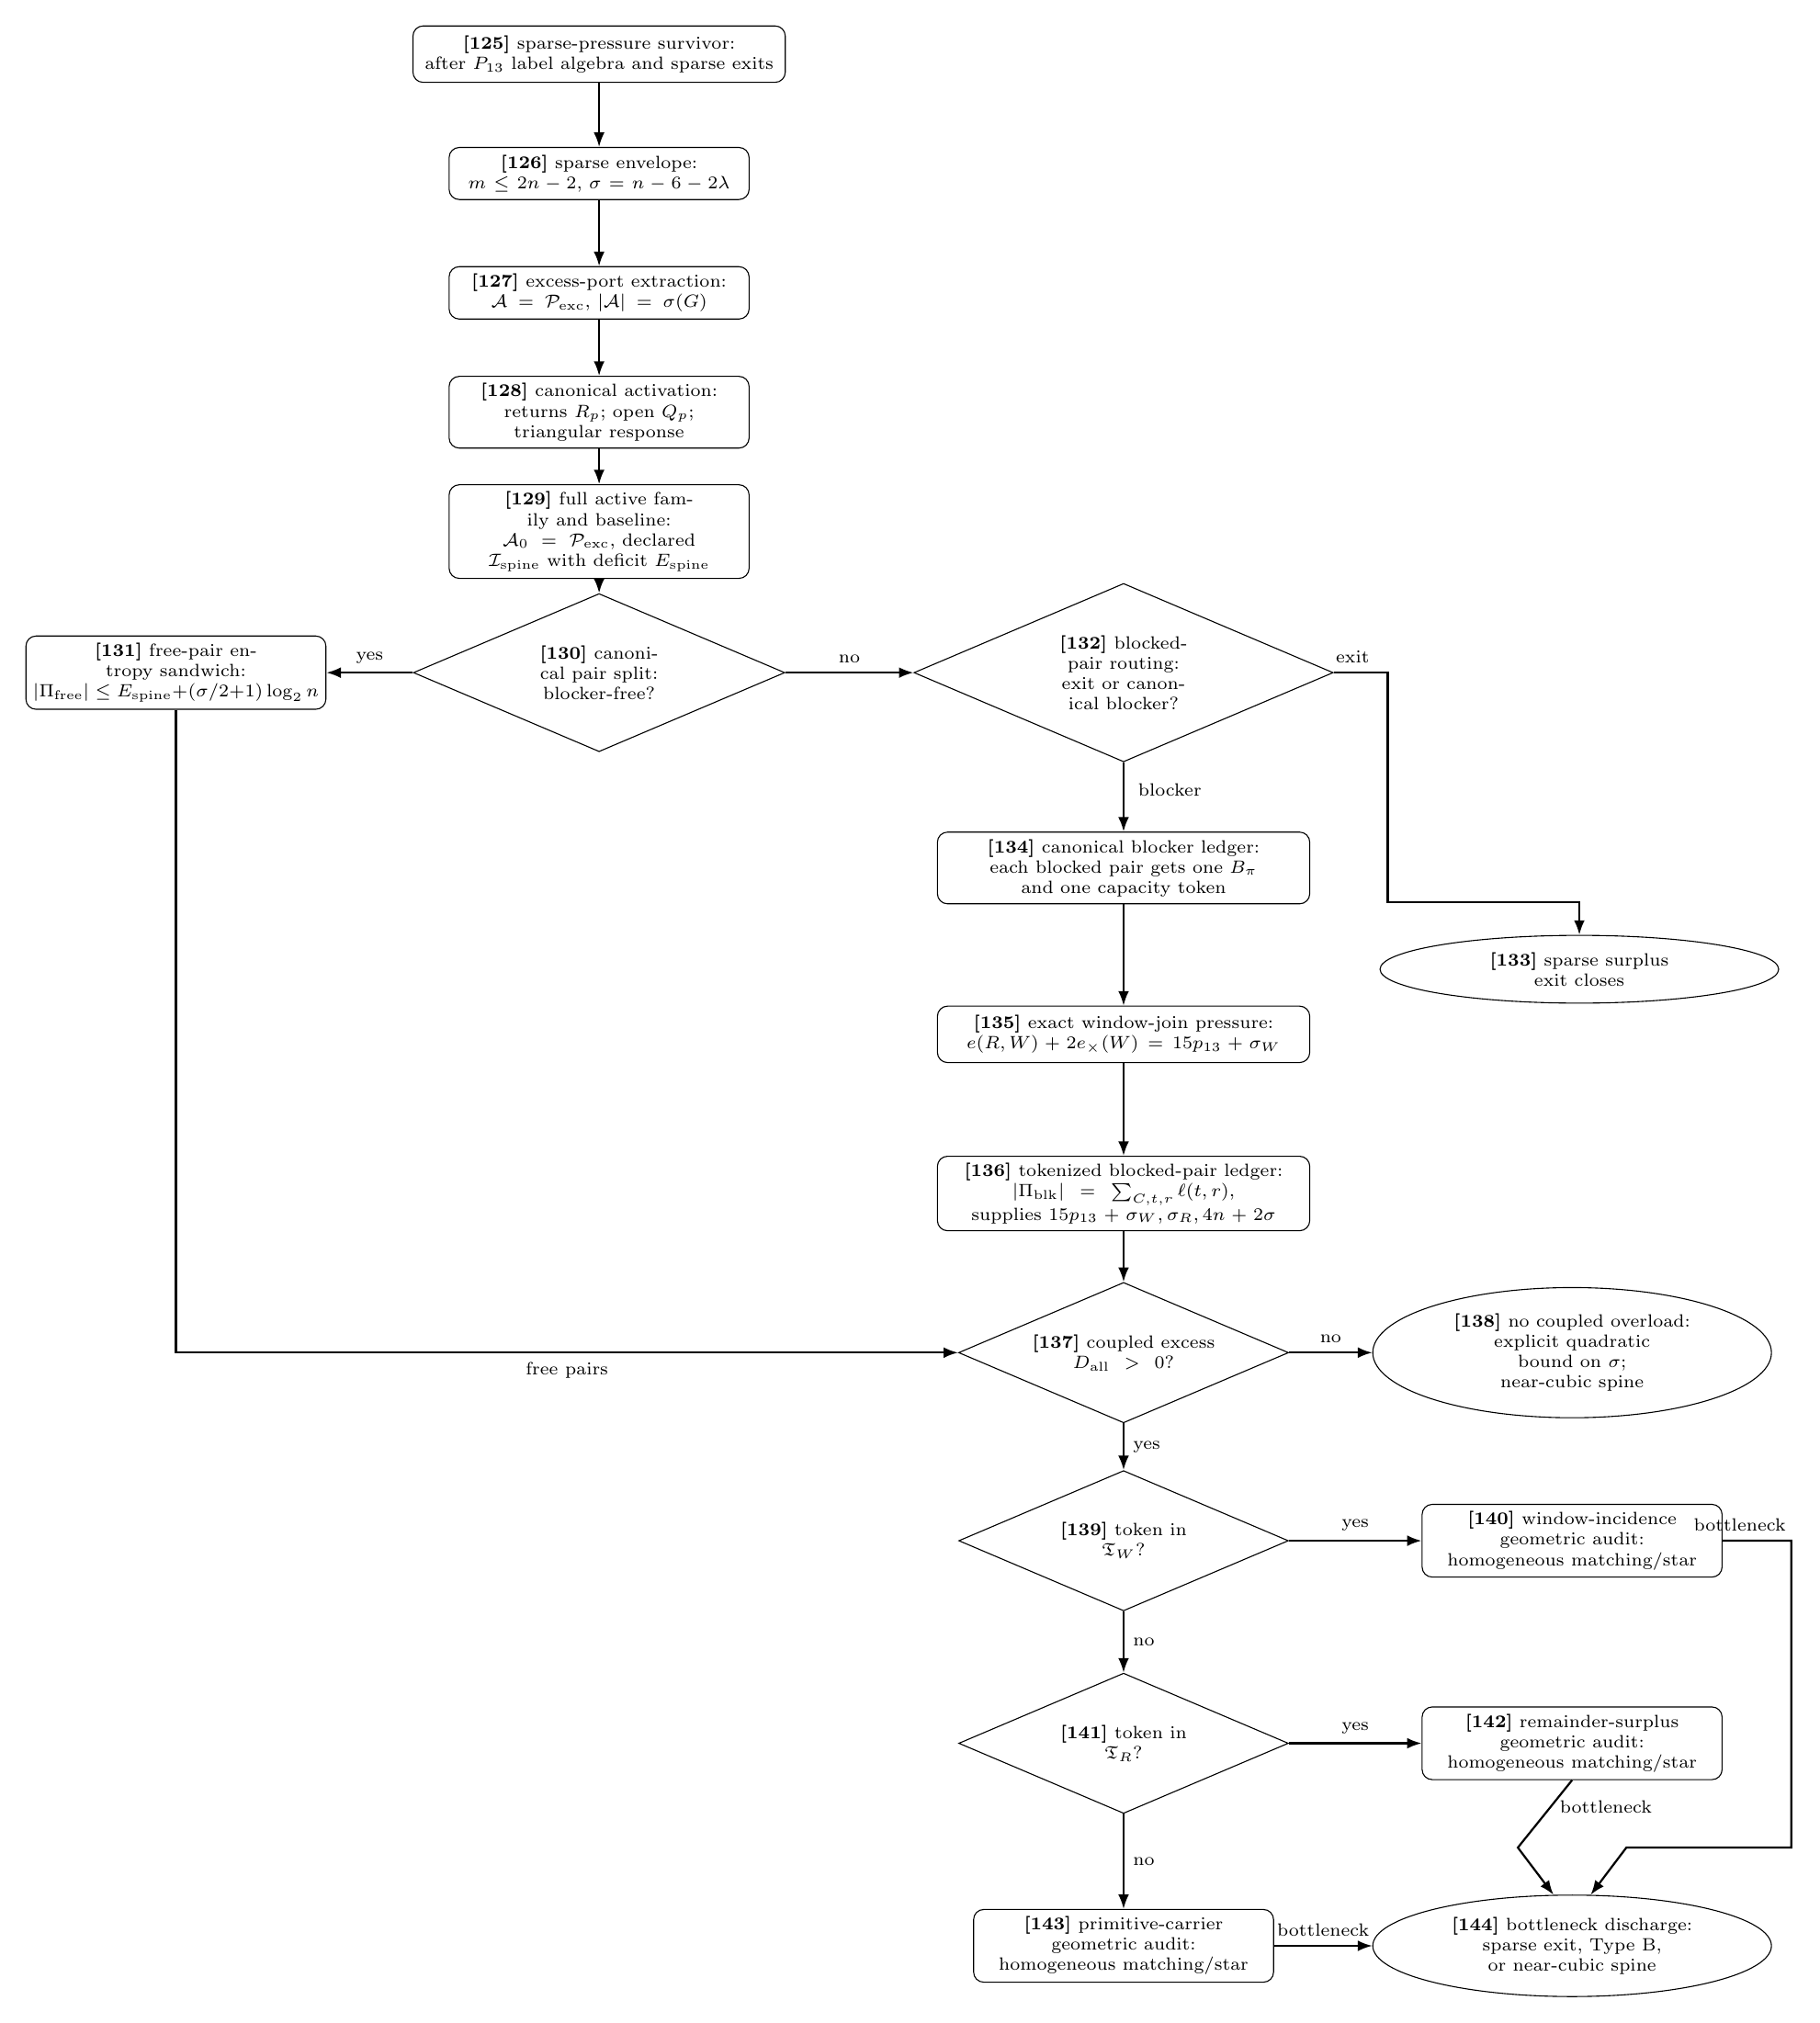
\begin{tikzpicture}[
box/.style={rectangle,rounded corners,draw,align=center,inner sep=2.8pt,text width=3.95cm,minimum height=0.72cm},
wide/.style={rectangle,rounded corners,draw,align=center,inner sep=2.8pt,text width=4.95cm,minimum height=0.78cm},
dec/.style={shape=diamond,draw,aspect=2.35,align=center,inner sep=1.4pt,text width=3.05cm,minimum height=1.25cm},
term/.style={ellipse,draw,align=center,inner sep=2.8pt,text width=3.70cm,minimum height=0.72cm},
arrow/.style={-{Latex[length=2mm]},thick},
every node/.style={font=\scriptsize}
]
\node[wide] (resid) at (-1.55,8.20) {\textbf{[125]}~sparse-pressure survivor:\\after \(P_{13}\) label algebra and sparse exits};
\node[box] (slack) at (-1.55,6.55) {\textbf{[126]}~sparse envelope:\\\(m\le2n-2\), \(\sigma=n-6-2\lambda\)};
\node[box] (extract) at (-1.55,4.90) {\textbf{[127]}~excess-port extraction:\\\(\mathcal A=\mathcal P_{\rm exc}\), \(|\mathcal A|=\sigma(G)\)};
\node[box] (activate) at (-1.55,3.25) {\textbf{[128]}~canonical activation:\\returns \(R_p\); open \(Q_p\); triangular response};
\node[box] (thin) at (-1.55,1.60) {\textbf{[129]}~full active family and baseline:\\\(\mathcal A_0=\mathcal P_{\rm exc}\), declared \(\mathcal I_{\rm spine}\) with deficit \(E_{\rm spine}\)};
\node[dec] (rankq) at (-1.55,-0.35) {\textbf{[130]}~canonical pair split:\\blocker-free?};
\node[box] (entropy) at (-7.40,-0.35) {\textbf{[131]}~free-pair entropy sandwich:\\\(|\Pi_{\rm free}|\le E_{\rm spine}+(\sigma/2+1)\log_2 n\)};
\node[dec] (depend) at (5.70,-0.35) {\textbf{[132]}~blocked-pair routing:\\exit or canonical blocker?};
\node[term] (exit) at (12.00,-4.45) {\textbf{[133]}~sparse surplus\\exit closes};
\node[wide] (blockers) at (5.70,-3.05) {\textbf{[134]}~canonical blocker ledger:\\each blocked pair gets one \(B_\pi\)\\and one capacity token};
\node[wide] (joinpress) at (5.70,-5.35) {\textbf{[135]}~exact window-join pressure:\\\(e(R,W)+2e_\times(W)=15p_{13}+\sigma_W\)};
\node[wide] (supplyq) at (5.70,-7.55) {\textbf{[136]}~tokenized blocked-pair ledger:\\\(|\Pi_{\rm blk}|=\sum_{C,t,r}\ell(t,r)\),\\supplies \(15p_{13}+\sigma_W,\sigma_R,4n+2\sigma\)};
\node[dec] (highload) at (5.70,-9.75) {\textbf{[137]}~coupled excess\\\(D_{\rm all}>0\)?};
\node[term] (nearclose) at (11.90,-9.75) {\textbf{[138]}~no coupled overload:\\explicit quadratic bound on \(\sigma\);\\near-cubic spine};
\node[dec] (wclass) at (5.70,-12.35) {\textbf{[139]}~token in\\\(\mathfrak T_W\)?};
\node[box] (wres) at (11.90,-12.35) {\textbf{[140]}~window-incidence\\geometric audit:\\homogeneous matching/star};
\node[dec] (rclass) at (5.70,-15.15) {\textbf{[141]}~token in\\\(\mathfrak T_R\)?};
\node[box] (rres) at (11.90,-15.15) {\textbf{[142]}~remainder-surplus\\geometric audit:\\homogeneous matching/star};
\node[box] (pres) at (5.70,-17.95) {\textbf{[143]}~primitive-carrier\\geometric audit:\\homogeneous matching/star};
\node[term] (capcontra) at (11.90,-17.95) {\textbf{[144]}~bottleneck discharge:\\sparse exit, Type B, or near-cubic spine};
\draw[arrow] (resid)--(slack);
\draw[arrow] (slack)--(extract);
\draw[arrow] (extract)--(activate);
\draw[arrow] (activate)--(thin);
\draw[arrow] (thin)--(rankq);
\draw[arrow] (rankq.west)--node[above]{yes}(entropy.east);
\draw[arrow] (rankq.east)--node[above]{no}(depend.west);
\draw[arrow] (depend.east)--node[above,pos=0.35]{exit}(9.35,-0.35)|-($(exit.north)+(0,0.45)$)--(exit.north);
\draw[arrow] (depend.south)--node[pos=0.40,right,xshift=2pt]{blocker}(blockers.north);
\draw[arrow] (blockers)--(joinpress);
\draw[arrow] (joinpress)--(supplyq);
\draw[arrow] (supplyq)--(highload);
\draw[arrow] (entropy.south)--(entropy.south|-highload.west)--node[below]{free pairs}(highload.west);
\draw[arrow] (highload.east)--node[above]{no}(nearclose.west);
\draw[arrow] (highload)--node[right]{yes}(wclass);
\draw[arrow] (wclass.east)--node[above]{yes}(wres.west);
\draw[arrow] (wclass)--node[right]{no}(rclass);
\draw[arrow] (rclass.east)--node[above]{yes}(rres.west);
\draw[arrow] (rclass)--node[right]{no}(pres);
\coordinate (wto144) at ($(capcontra.north)+(0.75,0.65)$);
\coordinate (rto144) at ($(capcontra.north)+(-0.75,0.65)$);
\draw[arrow] (wres.east)--node[above,pos=0.25]{bottleneck}++(0.95,0)|-(wto144)--(capcontra.70);
\draw[arrow] (rres.south)--node[right,pos=0.40]{bottleneck}(rto144)--(capcontra.110);
\draw[arrow] (pres.east)--node[above]{bottleneck}(capcontra.west);
\end{tikzpicture}%
}
\caption[Proof-dependency diagram, Part X]{Proof-dependency diagram, Part X.  This panel expands the sparse non-near-cubic branch [20].  Nodes [126]--[128] build the full active surplus family, and node [129] records the separate baseline-demand definition with its exact deficit.  A linear bound on that deficit is an additional downstream estimate, not a consequence of the definition.  Node [130] splits canonical pairs.  Free pairs are charged by the entropy sandwich [131], while blocked pairs pass through the blocker route [132]--[136]; the role fibres in [136] partition \(\Pi_{\rm blk}\), so this ledger has no double counting.  Node [137] is the coupled single-graph test of \cref{cor:coupled-single-graph-overload-budget,cor:numerical-single-graph-budget,prop:single-graph-sparse-pressure-routing}: all three token classes use the same \(n,p_{13},\sigma_W,\sigma_R\).  If \(D_{\rm all}=0\), the explicit quadratic bound routes to [138].  If \(D_{\rm all}>0\), the role-fibre excess enters the window-incidence, remainder-surplus, or primitive-carrier geometric audit [140], [142], [143].  Node [144] applies \cref{thm:homogeneous-overload-geometric-closure}: the bottleneck realizes a sparse surplus exit, produces Type B fan data, or is bounded by fixed homogeneous caps and routes to [138].}
\label{fig:proof-diagram-part-x}
\end{figure}

\clearpage

\begin{figure}[p]
\centering
\resizebox{0.96\textwidth}{!}{%
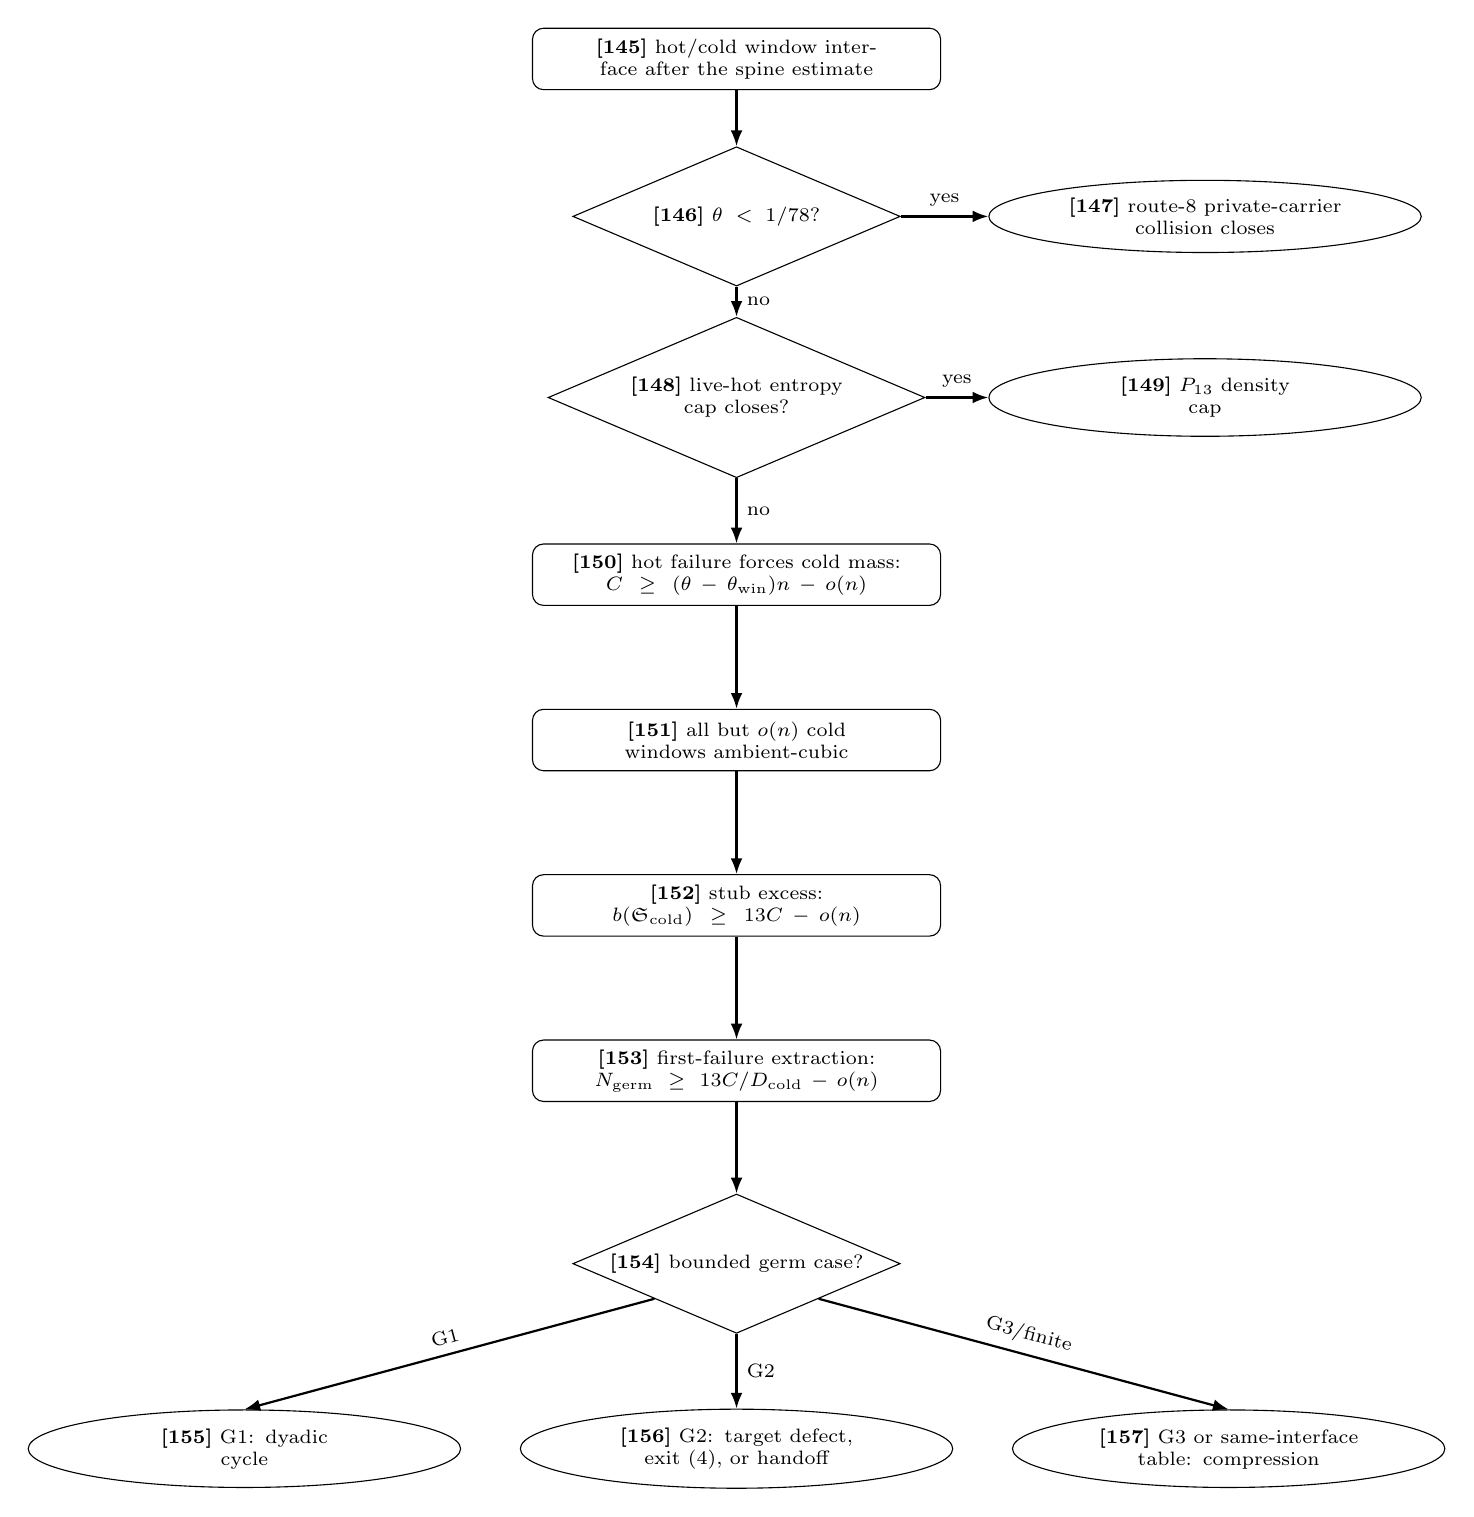
\begin{tikzpicture}[
box/.style={rectangle,rounded corners,draw,align=center,inner sep=2.6pt,text width=4.15cm,minimum height=0.72cm},
wide/.style={rectangle,rounded corners,draw,align=center,inner sep=2.6pt,text width=5.00cm,minimum height=0.78cm},
dec/.style={shape=diamond,draw,aspect=2.35,align=center,inner sep=1.4pt,text width=3.25cm,minimum height=1.25cm},
term/.style={ellipse,draw,align=center,inner sep=2.6pt,text width=3.70cm,minimum height=0.72cm},
arrow/.style={-{Latex[length=2mm]},thick},
every node/.style={font=\scriptsize}
]
\node[wide] (interface) at (0.00,7.50) {\textbf{[145]}~hot/cold window interface after the spine estimate};
\node[dec] (route8) at (0.00,5.50) {\textbf{[146]}~\(\theta<1/78\)?};
\node[term] (route8closed) at (5.95,5.50) {\textbf{[147]}~route-8 private-carrier\\collision closes};
\node[dec] (hot) at (0.00,3.20) {\textbf{[148]}~live-hot entropy\\cap closes?};
\node[term] (density) at (5.95,3.20) {\textbf{[149]}~\(P_{13}\) density\\cap};
\node[wide] (coldmass) at (0.00,0.95) {\textbf{[150]}~hot failure forces cold mass:\\\(C\ge(\theta-\theta_{\rm win})n-o(n)\)};
\node[wide] (cubic) at (0.00,-1.15) {\textbf{[151]}~all but \(o(n)\) cold windows ambient-cubic};
\node[wide] (stubs) at (0.00,-3.25) {\textbf{[152]}~stub excess:\\\(b(\mathfrak S_{\rm cold})\ge13C-o(n)\)};
\node[wide] (germs) at (0.00,-5.35) {\textbf{[153]}~first-failure extraction:\\\(N_{\rm germ}\ge13C/D_{\rm cold}-o(n)\)};
\node[dec] (germcase) at (0.00,-7.80) {\textbf{[154]}~bounded germ case?};
\node[term] (hit) at (-6.25,-10.15) {\textbf{[155]}~G1: dyadic\\cycle};
\node[term] (defect) at (0.00,-10.15) {\textbf{[156]}~G2: target defect,\\exit (4), or handoff};
\node[term] (compress) at (6.25,-10.15) {\textbf{[157]}~G3 or same-interface\\table: compression};
\draw[arrow] (interface)--(route8);
\draw[arrow] (route8.east)--node[above]{yes}(route8closed.west);
\draw[arrow] (route8)--node[right]{no}(hot);
\draw[arrow] (hot.east)--node[above]{yes}(density.west);
\draw[arrow] (hot)--node[right]{no}(coldmass);
\draw[arrow] (coldmass)--(cubic);
\draw[arrow] (cubic)--(stubs);
\draw[arrow] (stubs)--(germs);
\draw[arrow] (germs)--(germcase);
\draw[arrow] (germcase.south west)--node[above,sloped]{G1}(hit.north);
\draw[arrow] (germcase)--node[right]{G2}(defect);
\draw[arrow] (germcase.south east)--node[above,sloped]{G3/finite}(compress.north);
\end{tikzpicture}%
}
\caption[Proof-dependency diagram, Part XI]{Proof-dependency diagram, Part XI.  This panel expands the hot/cold \(P_{13}\)-window interface behind nodes [22]--[24].  If \(\theta<1/78\), the existing route-8 carrier inequality closes at [147].  Otherwise the live-hot entropy cap either yields the density cap [149], or the unpaid cold family has linear size [150].  On the near-cubic spine, only \(o(n)\) cold windows are non-cubic [151]; each ambient-cubic cold window has \(15\) external stubs, and after two corridor ends are absorbed it contributes \(13\) branch-excess units [152].  The first-failure extraction [153] assigns those selected half-edges to bounded cold germs and then uses the bounded-overlap constant \(D_{\rm cold}\) to obtain a linear disjoint family.  The germ trichotomy [154] has no terminal residual: G1 gives a dyadic cycle [155], G2 routes to target defect, exit \textup{(4)}, or the already existing handoff ledgers [156], and G3 together with the finite same-interface table gives a target-complete compression [157].}
\label{fig:proof-diagram-part-xi}
\end{figure}

\clearpage

\subsection*{Detailed dependency table}

The table records every named object in the proof-dependency diagram.  The \emph{Diagram node(s)} column uses the bracketed node numbers from the eleven numbered parts.  The Type A continuation node [63] is expanded in \cref{fig:proof-diagram-part-viii}, the Type B continuation node [64] is expanded in \cref{fig:proof-diagram-part-vi}, the route-8 residual node [109] is expanded in \cref{fig:proof-diagram-part-ix}, the surplus-pair accounting branch [20] is expanded in \cref{fig:proof-diagram-part-x}, and the hot/cold window interface is expanded in \cref{fig:proof-diagram-part-xi}.  The item numbers remain theorem-level bookkeeping and are not diagram-node identifiers.

{\scriptsize\setlength{\tabcolsep}{2pt}
\begin{longtable}{C{0.04\textwidth} L{0.13\textwidth} L{0.17\textwidth} L{0.25\textwidth} L{0.21\textwidth} L{0.12\textwidth}}
\toprule
\textbf{Item} & \textbf{Diagram node(s)} & \textbf{Node / theorem} & \textbf{Formal content} & \textbf{Failure route} & \textbf{Label} \\
\midrule
0 & [1]--[3] & Counterexample setup & $\delta(G)\ge3$ and no $C_{2^j}$ & If false, theorem holds for $G$ & \cref{def:counterexample} \\
1 & [4] & Minimality & choose minimal $(|V|,|E|)$ counterexample & smaller counterexample impossible & Assumption \\
2 & [5]--[7] & Edge-rooted target equivalence & no $C_{2^j}$ iff all $R_e(G)\cap\Mers=\varnothing$ & Mersenne return gives target cycle & \cref{lem:return-equivalence} \\
3 & [8] & No proper core & every proper subgraph has $\delta\le2$ & proper smaller counterexample & \cref{lem:no-proper-core} \\
4 & [9], [10], [67] & High-degree independence & $V_{\ge4}$ independent & high-high edge deletion & \cref{lem:deletion-critical} \\
5 & [11] & Boundaried graphs & atoms are $T$-boundaried supports & replacement formalism & \cref{def:boundaried-gluing} \\
6 & [11], [36], [37] & Boundary degree profiles & quotients fibrewise over $\mathbf d_\partial$ & otherwise target-defective & \cref{lem:degree-profile-fibres} \\
7 & [12], [36] & Context universality & target-complete identities work against every context & otherwise quotient defect & \cref{lem:context-universality} \\
8 & [13] & Replacement & smaller, at most as obstructing representative gives smaller counterexample & minimality contradiction & \cref{lem:replacement} \\
9 & [14], [38], [39] & Hereditary uncompressibility & no proper target-complete compression & replacement contradiction & \cref{cor:uncompressible} \\
10 & [31] & Target rank & independent coordinates realize $2^k$ states & entropy only counts independent coordinates & \cref{def:target-rank} \\
11 & --- & Skeleton budget & labelled edge sets dominate all canonical data & no extra auxiliary degrees of freedom & \cref{lem:skeleton-dominates} \\
12 & --- & Near-cubic budget & $B_{\mathrm{skel}}=\frac32 n\log_2n+o(n\log n)$ & budget scale & \cref{lem:near-cubic-budget} \\
13 & [15], [16] & $P_{13}$-free theorem & $P_{13}$-free $+\delta\ge3$ gives target cycle & forces induced $P_{13}$ & \cref{thm:p13free} \\
14 & [18] & $P_{13}$ label algebra & $399$ labels and relations $C_s$ & finite algebra basis & \cref{lem:labels} \\
15 & [21] & Curvature enumeration & $543958,432672,111286$ and $c_\Omega$ & verified finite computation & \cref{lem:curv-enum} \\
16 & [21] & Multi-scale window package & $c_{13}=118.108581006\ldots$ and \((c_{13}-o(1))p_{13}\log_2 n\) independently target-testable window coordinates & controls $P_{13}$ packing density & \cref{lem:p13-window-package}; \cref{app:curv-code} \\
17 & [22]--[24] & $P_{13}$ density bound & after surplus-token routing supplies \cref{def:near-cubic-spine}, $\theta\le\theta_{\rm win}+o(1)$; high entropy gives $\theta\le0.01198542083\ldots+o(1)$ & window entropy overflow / window-only cap & \cref{lem:p13-window-package}, \cref{prop:p13-density} \\
18 & [145]--[157] & Hot/cold window branch & if \(\theta<1/78\), route 8 closes; otherwise hot failure forces \(C\ge(\theta-\theta_{\rm win})n-o(n)\), \(b(\mathfrak S_{\rm cold})\ge13C-o(n)\), and \(N_{\rm germ}\ge13C/D_{\rm cold}-o(n)\); bounded germs route to hit, defect, handoff, route 8, same-interface table, or compression & no terminal cold residual after the spine estimate & \cref{def:cold-window-ledger,def:surviving-cold-branch,lem:hot-failure-cold-mass,def:cold-skeleton-excess,lem:cold-window-stub-excess,lem:cold-short-self-return-filter,def:cold-bounded-germ,def:cold-corridor-first-failure,lem:cold-corridor-first-failure,lem:cold-germ-extraction,lem:cold-bounded-germ-trichotomy,def:cold-same-interface-table,lem:cold-same-interface-table,lem:cold-increment-arithmetic,thm:cold-branch-quantitative-closure} \\
19 & [17], [25]--[27] & Remainder $R$ & componentwise $P_{13}$-free and large & maximality of packing & \cref{sec:remainder} \\
20 & [28] & Positive deficiency & $\defp(X)=\sum_v\max(0,3-d_X(v))$ & high degree cannot cancel deficient vertices & \cref{def:deficiency-surplus} \\
21 & [29] & External-incidence supply & $\defp(R)\le15p_{13}+o(n)$ and hence $\defp(R)-\sigma_R\le15p_{13}+o(n)$ & few windows give small supply & \cref{lem:stub-positive} \\
22 & [30] & Wedge lower bound & componentwise \(W_2(C)\ge3|V(C)|-2\defp(C)\); with \(\defp(R)\le(\tau_{\rm win}+o(1))|R|\), this gives \(W_2(R)\ge\omega_{\rm win}|R|-o(|R|)\); high entropy gives \(\omega|R|-o(|R|)\) & degree-count proof & \cref{lem:wedge-lower} \\
23 & [31] & Curvature target-rank & $r_\Omega(R)$ counts independent curvature tests via functional admissible rank quotients of exact response profiles & raw tests are not charged directly; closed empty-boundary data stay label-injective & \cref{def:exact-response-profile,def:admissible-rank-quotient,def:functional-rank-quotient,def:curvature-target-rank} \\
24 & [32], [33], [35]--[37] & Localization of curvature dependence & rank drop gives a finite functional target-dependence and routes to target defect/admissible compression/support & dependence cannot be silent locally & \cref{lem:target-rank-circuit,lem:curvature-dependence-routing} \\
25 & [35]--[37] & Separated wedge testers & identical separated wedge balls are context-universal or defective & supports full-rank forcing & \cref{lem:separated-testers} \\
26 & [40]--[42] & Proper delocalization support & enlarged $Z\subsetneq G$ gives target defect or target-complete proper-support compression & context defect or replacement contradiction & \cref{lem:proper-smearing} \\
27 & [44] & Repair identity & $s=p-2+2\beta_Z-\sigma_Z$ & global delocalization rank barrier & \cref{lem:smearing-support-repair} \\
28 & [43], [45] & No silent global delocalization & $Z=G$ gives target-defect, smaller closed counterexample, or exact label-injective global data & no global silent rank reduction & \cref{def:exact-response-profile,def:admissible-rank-quotient,lem:no-silent-global-smearing} \\
29 & [34], [46], [47] & Full curvature rank & $r_\Omega(R)\ge W_2(R)-o(W_2)$ & if rank drops, contradiction & \cref{lem:full-rank} \\
30 & [48] & Forced curvature cost & $c_\Omega W_2(R)\ge K_{\rm win}|R|-o(|R|)$; high entropy gives $K|R|-o(|R|)$ & finite-size cost & \cref{cor:forced-curvature-cost} \\
31 & [49] & Per-vertex remainder entropy & $\eta(R)=\log_2|\mathcal G(R)|/|R|$ & separates high-/low-entropy remainder regimes & \cref{def:remainder-entropy} \\
32 & [49], [50] & Dominant local type & low-entropy remainder has dominant rooted type & otherwise too many labelled remainder states & \cref{lem:dominant-type} \\
33 & [51], [52] & Translates independent & separated dominant wedges are independently target-testable & otherwise rank-forcing applies & \cref{lem:translates-independent} \\
34 & [50]--[54] & Two-budget routing & high-entropy branch uses window entropy; repetitive low-entropy branch gives positive curvature rank; nonrepetitive low-entropy branch is routed forward & prevents entropy overcounting & \cref{prop:two-budget} \\
35 & [53], [54] & Finite threshold $\Theta(n)$ & high-$\theta$ branch closed by entropy cap & small-budget closure & \cref{def:Theta}, \cref{prop:entropy-high-theta} \\
36 & [55]--[57] & Net-deficiency cap & large-budget branch has $\Delta_{\mathrm{net}}\le\tau_{\rm win}+o(1)<1/4$ & very low net deficiency required & \cref{sec:large-budget} \\
37 & [58] & Net charge & $\No(X)=\defp(X)-\sigma(X)-|X|/4$ & failure localizes to negative support & \cref{def:net-charge} \\
38 & [59]--[62] & Net charge localization & negative global net charge gives connected negative support & Type A/Type B split & \cref{lem:netcharge-superadd}, \cref{prop:negative-net-charge} \\
39 & [63], [86]--[109] & Type A obstruction & bounded low-deficiency $P_{13}$-free atom split into closed saturated exits, target-defect peeling, Type B handoff, unsaturated discharging, and the route-8 trace-basin branch & raw $4/8/12$ thresholds, exits 1--3, 5, and 6 close, exit 4 peels exactly one target-defective routed load, exit 7 hands off to Type B through connector-germ routing, cubic-switch absorption, and high-degree handoff, unsaturated $3/7/11$ discharging, route-8 burden $S_{\rm sil}^{\rm exc}(X)\ge4D_A(X)$, declared $u$-supported response algebra, canonical minimal target-complete carrier core, cut parity, zero/one essential-carrier collapse, private-carrier reduction to a two-carrier entry, carrier-deletion witnesses, and the terminal no-go theorem & \cref{def:typeA-receiver-load}, \cref{def:typeA-continuation-classes}, \cref{def:typeA-saturated-exits}, \cref{def:typeA-exit4-peeling}, \cref{lem:typeA-continuation-routing}, \cref{lem:typeA-cubic-switch-absorption}, \cref{lem:typeA-high-degree-handoff}, \cref{lem:typeA-exit4-peeling-charge}, \cref{lem:typeA-unpeeled-visible-routing}, \cref{lem:typeA-unpeeled-silent-routing}, \cref{lem:typeA-exit4-residual-routing}, \cref{lem:typeA-exits-discharged}, \cref{lem:typeA-threshold-algebra}, \cref{lem:typeA-saturated-handoff}, \cref{lem:typeA-unsaturated-discharge}, \cref{lem:typeA-exclusion}, \cref{def:typeA-silent-core-residual}, \cref{def:typeA-large-budget-deficit}, \cref{def:typeA-route8-carriers}, \cref{lem:typeA-route8-burden}, \cref{lem:typeA-carrier-cut-parity}, \cref{lem:typeA-one-terminal-collapse}, \cref{def:typeA-carrier-deletion-witness}, \cref{lem:typeA-essential-deletion-witness}, \cref{lem:typeA-deletion-witness-declared}, \cref{lem:typeA-two-carrier-deletion-canonical}, \cref{lem:typeA-carrier-deletion-exit}, \cref{def:typeA-terminal-two-carrier}, \cref{thm:typeA-two-carrier-nogo}, \cref{prop:typeA-route8-closure-from-nogo} \\
40 & [64]--[85], [108] & Type B obstruction & degree-$4$ fan-safe surplus support, degree-greater-than-four heavy-center side branch, and decorated handoff fan data & degree-four centers give either a fan-compatible open pair or two triangular ports; heavy centers reduce to a fan-compatible open pair or three triangular ports; in either case two fan-closed ports give a positive-deficit Type B fan; triangular shoulders have only central/cross/outside completion landings; certificate-marked fans have the local cap and local certificate/B1 ledger; fan-certificate residual centers go to fan-mass; B2 failures form minimal overlap obstructions; on the derived spine branch all Type B bridge residual mass is bounded by the global surplus budget & \cref{def:decorated-fan-envelope}, \cref{lem:decorated-fan-admissibility}, \cref{def:marked-typeB-fan}, \cref{def:heavy-center-triangular-port}, \cref{def:triangular-fan-core}, \cref{lem:heavy-neighbourhood-normal-form}, \cref{def:fan-compatible-open-ports}, \cref{lem:same-center-open-port-compatibility}, \cref{cor:degree-four-local-activation}, \cref{lem:heavy-center-triangular-alternative}, \cref{cor:heavy-center-local-dichotomy}, \cref{lem:triangular-shoulder-completion}, \cref{lem:triangular-port-return}, \cref{lem:triangular-first-landing}, \cref{lem:triangular-cross-shoulder}, \cref{def:fan-closed-port}, \cref{lem:compatible-pair-fan-closure}, \cref{prop:fan-closed-port-typeB-routing}, \cref{cor:compatible-pair-typeB-routing}, \cref{prop:triangular-port-typeB-routing}, \cref{def:typeB-window-incidence-profile}, \cref{def:typeB-hybrid-incidence}, \cref{def:closed-fan-window-pair}, \cref{def:direct-cycle-free-closed-pair}, \cref{lem:typeB-direct-fan-window-cycles}, \cref{lem:typeB-two-window-cycles}, \cref{lem:typeB-multiclosed-budget}, \cref{lem:typeB-hybrid-incidence-budget}, \cref{lem:typeB-hybrid-B1}, \cref{def:typeB-ledger-carriers}, \cref{def:typeB-candidate-ledger}, \cref{def:typeB-overlap-obstruction}, \cref{lem:typeB-bridge-to-overlap}, \cref{lem:typeB-global-local-reflection}, \cref{prop:typeB-global-local-bridge}, \cref{def:typeB-bridge-statements}, \cref{prop:typeB-bridge-reduction}, \cref{def:typeB-multiclosed-residual}, \cref{lem:typeB-exclusion}, \cref{def:typeB-residual-mass}, \cref{lem:decorated-envelope-with-route8-core}, \cref{lem:typeB-bridge-deficit-bound}, \cref{lem:typeB-bridge-with-route8-core}, \cref{prop:typeB-bridge-sublinear} \\
41 & [76], [85] & Branch-closure theorem & After surplus-token routing has supplied the near-cubic spine estimate, pure Type A outside route 8 closes locally and Type B bridge residual centers and B2 failures are sublinear globally & outside explicit Type A route 8 and Type B bridge residuals, the entropy-admissible branch has no survivor & \cref{thm:branch-kill} \\
42 & [123] & Large-budget pressure descent & The remaining linear Type A deficit is placed in the unified target-defect/route-8 ledger; every target-defect two-carrier entry is canonical exit-(4) peel data, and finite descent removes it & the terminal large-budget branch can survive only through a two-carrier route-8 entry, which is then routed to node [124] & \cref{def:typeA-unified-negative}, \cref{def:typeA-pressure-ledger}, \cref{def:typeA-peeling-reduced-ledger}, \cref{lem:typeA-peeling-reduced-reduction}, \cref{lem:typeA-pressure-is-exit4-peel}, \cref{lem:typeA-exit4-finite-descent}, \cref{thm:large-budget-route8-only} \\
43 & [110]--[124] & Route-8 exit closure & after target-defect descent, the route-8 burden gives $N_{\rm basin}\ge4D_A$; canonical carrier cores close zero/one-essential-core entries; absence of a two-carrier entry forces incompatible private-carrier upper and lower bounds; a two-carrier entry supplies a terminal obstruction with declared deletion witnesses & node [124] rules out the terminal two-carrier obstruction because the two-carrier condition places each declared deletion quotient in the canonical exit-(4) family, while exit (4) is absent in a true route-8 residual & \cref{def:typeA-large-budget-deficit}, \cref{def:typeA-route8-carriers}, \cref{def:typeA-true-route8-residual}, \cref{lem:typeA-route8-burden}, \cref{lem:typeA-carrier-cut-parity}, \cref{lem:typeA-one-terminal-collapse}, \cref{prop:typeA-route8-carrier-reduction}, \cref{def:typeA-carrier-deletion-witness}, \cref{lem:typeA-essential-deletion-witness}, \cref{lem:typeA-deletion-witness-declared}, \cref{lem:typeA-two-carrier-deletion-canonical}, \cref{lem:typeA-carrier-deletion-exit}, \cref{def:typeA-terminal-two-carrier}, \cref{thm:typeA-two-carrier-nogo}, \cref{prop:typeA-route8-closure-from-nogo}, \cref{thm:large-budget-route8-only} \\
44 & --- & Enumeration appendix & reproduces all finite constants including $c_{13}$ & constants are checkable & \cref{app:curv-code} \\
45 & [19], [20] & Non-near-cubic surplus branch & every survivor of the sparse surplus exits has the full active-demand family and, after an \(O(n)\)-deficit baseline demand is fixed, satisfies the exact capacity-token budget; the geometric same-token bottleneck lemma gives fixed homogeneous caps unless the load realizes a sparse surplus exit or ordinary Type B fan data, and the caps give \(\sigma(G)=O(\sqrt n)\) & derives the near-cubic spine before the normalized entropy budget is used, except for branches that are already routed to sparse exits or to the Type B fan ledger; blocker-free pair responses are charged by the exact cubic-baseline sandwich and the spine lower-bound deficits, while blocked pairs are assigned to capacity tokens; the exact token-fibre budget gives the load forced by any attempted violation, and \cref{lem:same-token-bottleneck-routing} turns a large homogeneous fibre into a geometric first-separator/fan route & \cref{lem:sparse-upper-envelope}, \cref{lem:sparse-slack-surplus}, \cref{def:named-surplus-exits}, \cref{def:active-surplus-demands}, \cref{lem:surviving-active-family}, \cref{def:surplus-blockers}, \cref{def:canonical-blocker-ledger}, \cref{lem:canonical-blocker-ledger-no-overcount}, \cref{def:primitive-sparse-blocker-carrier}, \cref{lem:primitive-carrier-supply}, \cref{def:capacity-token-ledger}, \cref{lem:capacity-token-supply}, \cref{lem:token-ledger-no-overcount}, \cref{def:same-token-patterns}, \cref{def:same-token-blocker-roles}, \cref{def:same-token-routing-germs}, \cref{lem:same-token-matching-star}, \cref{lem:same-token-homogeneous-extraction}, \cref{lem:same-token-bottleneck-routing}, \cref{thm:homogeneous-overload-geometric-closure}, \cref{cor:homogeneous-same-token-caps-close}, \cref{def:baseline-spine-demand}, \cref{lem:exact-cubic-baseline-budget}, \cref{lem:incremental-skeleton-room}, \cref{prop:sparse-entropy-sandwich}, \cref{prop:sparse-entropy-sandwich-with-blockers}, \cref{thm:tokenized-surplus-accounting-closure}, \cref{def:window-remainder-surplus-split}, \cref{lem:exact-window-join-identity}, \cref{cor:global-window-join-pressure}, \cref{prop:nonnear-cubic-sharp-overload-routing} \\
46 & [125]--[128] & Ordered surplus activation & a sparse-pressure survivor yields the full excess-slot ledger; the ordered CT6 audit scans high centres and either returns the first non-cubic incident endpoint or certifies every centre active & deletion criticality rules out the failure terminal; the ledger weight is exactly \(\sum_v(d(v)-3)=\sigma(G)\) & \cref{lem:sparse-excess-port-extraction}, \cref{lem:sparse-port-activation}, \cref{lem:surviving-active-family} \\
46a & [129] & Baseline spine demand & after the active family has been established, record a declared baseline demand and its exact deficit & a linear deficit bound is a separate downstream estimate, not a premise of the CT6 activation audit or a consequence of the definition & \cref{def:baseline-spine-demand} \\
46b & [64]--[69], [78], [130] & Finite local-port audit & four-cycle avoidance, selected-port classification, center-fibre overload, overload-only adjacency-response comparison, the exact two-shoulder ledger, the nonadjacent same-center fan-compatibility implication, the all-incident-port high-center dichotomy, and triangular shoulder-completion bookkeeping & scans only declared vertex and neighbour schedules; it does not materialize port pairs, paths, or subsets, and does not establish the later Type B/free-blocked routing & \cref{rem:finite-selected-port-audit,lem:heavy-neighbourhood-normal-form,def:heavy-center-triangular-port,lem:same-center-open-port-compatibility,lem:heavy-center-triangular-alternative,cor:heavy-center-local-dichotomy,lem:triangular-shoulder-completion} \\
47 & [130]--[132] & Free/blocked pair split & pair-response coordinates split into blocker-free and blocked pairs; free pairs are charged by the entropy sandwich & blocked-pair debt is the only branch passed to the token ledger & \cref{def:sparse-canonical-connector}, \cref{def:sparse-pair-response}, \cref{lem:sparse-pair-dependence-exit}, \cref{prop:sparse-entropy-sandwich-with-blockers} \\
48 & [132]--[136] & Blocker and token ledger & canonical blockers, primitive carriers, and capacity tokens count blocked pairs exactly once & [136] is the exact token-fibre partition and no-overcounting closure & \cref{def:surplus-blockers}, \cref{lem:sparse-blocker-values-finite}, \cref{def:canonical-sparse-blocker-order}, \cref{def:canonical-blocker-ledger}, \cref{lem:canonical-blocker-ledger-no-overcount}, \cref{def:primitive-sparse-blocker-carrier}, \cref{lem:primitive-carrier-supply}, \cref{def:capacity-token-ledger}, \cref{lem:capacity-token-supply}, \cref{lem:token-ledger-no-overcount} \\
49 & [135], [136] & Window-join pressure & the exact packed-window join identity supplies \(15p_{13}+\sigma_W\) and the surplus-aware window-stub pressure & supplies the window/remainder capacity side of the token ledger & \cref{def:window-remainder-surplus-split}, \cref{lem:exact-window-join-identity}, \cref{cor:global-window-join-pressure}, \cref{rem:surplus-pair-sharp-frontier} \\
50 & [137]--[143] & Coupled high-load split & the single-graph high-load test splits the forced homogeneous pattern into window-incidence, remainder-surplus, and primitive-carrier token classes & [139]--[143] are the three token-class audits & \cref{def:same-token-patterns}, \cref{def:same-token-blocker-roles}, \cref{def:homogeneous-token-charge}, \cref{lem:exact-surplus-pair-charge-partition}, \cref{lem:same-token-matching-star}, \cref{thm:sharp-classwise-homogeneous-token-budget}, \cref{thm:tokenized-surplus-accounting-closure} \\
51 & [140], [142]--[144] & Geometric bottleneck discharge & a large same-token fibre gives a homogeneous matching or star, then realizes a sparse exit, Type B fan data, or fixed homogeneous caps & [144] sends the branch to a sparse exit, Type B, or [138] & \cref{def:same-token-routing-germs}, \cref{lem:same-token-bottleneck-routing}, \cref{thm:homogeneous-overload-geometric-closure}, \cref{cor:homogeneous-same-token-caps-close} \\
\bottomrule
\end{longtable}
}

\subsection*{The constraint ledger}

The reduction tracks a fixed list of \emph{invariants}: numbered structural constraints that a minimal counterexample $G$ must satisfy, together with the entropy or deficiency \emph{budget} each one spends and the labeled results that introduce or consume it.  Throughout, $G$ is the lexicographically minimal counterexample, so $\delta(G)\ge3$ and $R_e(G)\cap\Mers=\varnothing$ for every oriented edge.  Budgets quoted in the skeleton normalization $B_{\mathrm{skel}}=\tfrac32 n\log_2 n+o(n\log n)$ are used only after \cref{prop:nonnear-cubic-sharp-overload-routing} has either routed the non-near-cubic sparse-surplus branch to a closed ledger or supplied the near-cubic spine estimate of \cref{def:near-cubic-spine}.  We write $\theta=p_{13}/n$, with densities taken per $|R|$ or per $n$ as noted.  We recall the recurring parameters $\beta=m-n+1$ (cycle rank), $\lambda=2n-3-m$ (sparsity rank), $\sigma=2m-3n$ (surplus above cubic), and, for an atom $C$, its deficiency $d(C)=\sum_{v}(3-d_C(v))$.  The ledger is organized into blocks; the reverse (result~$\to$~invariant) view is given in the next subsection.

\paragraph{External inputs (black boxes).}
The argument imports four external results; only the first enters the final
proof as a load-bearing black box.  The non-near-cubic surplus branch is
internal: it uses the
free/blocked pair split, the capacity-token ledger, and the same-token
bottleneck routing of \cref{lem:same-token-bottleneck-routing}.

{\small
\begin{longtable}{L{0.17\textwidth} L{0.28\textwidth} L{0.27\textwidth} L{0.20\textwidth}}
\toprule
\textbf{Input} & \textbf{Statement used} & \textbf{Constraint it imposes on $G$} & \textbf{Used by} \\
\midrule
\endhead
HSS $P_{13}$-free theorem (\cref{thm:p13free}) & $P_{13}$-free $+\ \delta\ge3\ \Rightarrow$ a power-of-two cycle & $G$ must contain an induced $P_{13}$; after removing a maximal disjoint $P_{13}$ family, every remainder component is $P_{13}$-free and boundary-deficient & \cref{cor:p13-exists}, \cref{lem:stub-positive}, invariants 20--24, entire remainder analysis \\
Bondy--Vince / Gao--Ma & Few sub-cubic vertices force two cycle lengths differing by $1$ or $2$; quiet-block cap $|X|<5b(X)^2$ & Large almost-cubic atoms must export close cycle lengths or pay quadratic boundary & Appendix resilience bookkeeping \\
Kleitman--West max-leaf & $\delta\ge3\ \Rightarrow$ spanning tree with $\ge n/4+2$ leaves & Cotree fundamental cycles must avoid Mersenne tree distances & Appendix tree--cotree profile bookkeeping \\
Degree-3-critical / $1$--$3$ tree literature & Extremal graphs with no proper $\delta\ge3$ subgraph have $1$--$3$ tree / leaf-path structure & Guides the repair-network identity & Appendix marked length-rank bookkeeping \\
\bottomrule
\end{longtable}
}

\paragraph{Block I: minimality and target algebra (invariants 1--8).}
{\scriptsize\setlength{\tabcolsep}{3pt}
\begin{longtable}{C{0.022\textwidth} L{0.135\textwidth} L{0.115\textwidth} L{0.235\textwidth} L{0.085\textwidth} L{0.29\textwidth}}
\toprule
\textbf{\#} & \textbf{Invariant} & \textbf{Node (first tracked)} & \textbf{Constraint on $G$} & \textbf{Budget} & \textbf{Lemmas/theorems using it} \\
\midrule
\endhead
1 & Mersenne-return target algebra & Target {[5]} & No dyadic cycle $\iff R_e(G)\cap\Mers=\varnothing$ for every directed edge & --- (defines the target predicate) & \cref{lem:return-equivalence} (states it); \cref{def:dyadic-safe}; consumed by \emph{every} quotient/atom/profile result: \cref{lem:degree-profile-fibres}, \cref{lem:context-universality}, \cref{lem:replacement}, \cref{cor:uncompressible}, invariants 30--38 \\
2 & Minimal proper-subgraph condition & Core {[8]} & Every proper subgraph has $\delta\le2$ & --- & \cref{lem:no-proper-core} (states it); underlies \cref{lem:cycle-rank}, \cref{lem:replacement} \\
3 & Edge-deletion criticality & Delete {[9]} & Every edge touches a degree-$3$ vertex & --- & \cref{lem:deletion-critical} (states it) \\
4 & High-degree independence & High-degree {[10]} & $V_{\ge4}$ is independent & --- & \cref{lem:deletion-critical} (corollary); used by \cref{lem:typeB-exclusion} (fan aggregation), invariant 16 \\
5 & No passive degree-$2$ storage & Counterex. {[2]} & Final $G$ has no degree-$2$ vertex; frontier degree-$2$ must be compensated & --- & Motivates $1$--$3$ networks; \cref{lem:stub-positive}, repair-network auxiliaries \\
6 & Replacement dominance & Replace {[13]} & If $X'$ is smaller with $\profile(X')\subseteq\profile(X)$, replacing $X$ by $X'$ gives a smaller counterexample & --- & \cref{lem:replacement} (states it); \cref{lem:degree-profile-fibres}, \cref{lem:context-universality} feed it; \cref{cor:uncompressible} derives from it \\
7 & Lumpability defect & Univ. {[12]} & A quotient is valid only if it preserves target-hitting under every outside context & --- & \cref{lem:context-universality} (states it); used in final spine step~7; \cref{lem:labels} (defect at path-lengths $1,2,3$) \\
8 & Hereditary target-uncompressibility & Uncomp. {[14]} & No proper atom admits a nontrivial target-complete compression & --- & \cref{cor:uncompressible} (states it); \textbf{the contradiction lever} in final spine step~7; consumed by \cref{lem:typeA-exclusion}, \cref{lem:typeB-exclusion}, invariant 29 \\
\bottomrule
\end{longtable}
}

\paragraph{Block II: degree, rank, sparsity (invariants 9--19).}
{\scriptsize\setlength{\tabcolsep}{3pt}
\begin{longtable}{C{0.022\textwidth} L{0.135\textwidth} L{0.115\textwidth} L{0.235\textwidth} L{0.085\textwidth} L{0.29\textwidth}}
\toprule
\textbf{\#} & \textbf{Invariant} & \textbf{Node (first tracked)} & \textbf{Constraint on $G$} & \textbf{Budget} & \textbf{Lemmas/theorems using it} \\
\midrule
\endhead
9 & Minimum edge count & Counterex. {[2]} & $m\ge\lceil 3n/2\rceil$ & --- & \cref{lem:cycle-rank}; near-cubic specialization \cref{lem:near-cubic-budget} \\
10 & Sparse upper envelope & Core {[8]} & $m\le 2n-2$ & --- & \cref{lem:sparse-upper-envelope,lem:variable-edge-budget}; Laman identity (invariant 12) \\
11 & Cycle-rank pressure & Minimality {[4]} & $\beta=m-n+1\ge n/2+1$ (up to parity) & --- & \cref{lem:cycle-rank} (states it); feeds 12, 13 \\
12 & Laman slack identity & Rank ids {[4]} & $\beta+\lambda=n-2$ & --- & \cref{def:remainder-entropy}, two-budget split; standing notation; \cref{lem:near-cubic-budget} \\
13 & Surplus--rank relation & Rank ids {[4]} & $\sigma=2\beta-n-2$, $\lambda=n/2-3-\sigma/2$ & --- & Near-cubic accounting; \cref{lem:netcharge-superadd} (via $\sigma$) \\
14 & High-degree surplus bound & Surplus branch {[125]--[144]} supplies spine estimate & $\sigma=O(\sqrt n)$ for survivors after sparse exits and Type B handoff data are routed, because \cref{thm:homogeneous-overload-geometric-closure} supplies fixed role-homogeneous same-token caps for all three token classes & $\sigma$-budget: $O(\sqrt n)$ & \cref{def:near-cubic-spine}, \cref{def:same-token-patterns}, \cref{def:same-token-blocker-roles}, \cref{def:same-token-routing-germs}, \cref{lem:same-token-matching-star}, \cref{lem:same-token-homogeneous-extraction}, \cref{lem:same-token-bottleneck-routing}, \cref{thm:homogeneous-overload-geometric-closure}, \cref{cor:homogeneous-same-token-caps-close}, \cref{prop:nonnear-cubic-sharp-overload-routing}; \cref{prop:negative-net-charge} \\
15 & Near-cubic edge count & Surplus branch {[125]--[144]} supplies spine estimate & $m=\tfrac32 n+O(\sqrt n)$, $\bar d=3+O(n^{-1/2})$ for the same survivors & sets $B_{\mathrm{skel}}$ coefficient $\tfrac32$ & \cref{def:near-cubic-spine}, \cref{thm:homogeneous-overload-geometric-closure}, \cref{prop:nonnear-cubic-sharp-overload-routing}, \cref{lem:near-cubic-budget}, \cref{lem:skeleton-dominates}, all entropy inequalities \\
16 & Certificate-marked fan degree & High-degree {[67]} & certificate-marked Type B fans satisfy $d_G(h)\le8$; fan-certificate residual centers are charged by $\sum_h(d_G(h)-3)$ & label-packing cap plus $\sigma$-budget & \cref{lem:fan-certificate,lem:typeB-exclusion,prop:typeB-bridge-sublinear}; related to invariant 4 \\
17 & Spectral feasibility mask & Spectral {[70]} & $A(H)\le M$, $\delta(H)\ge3\ \Rightarrow\rho(M)\ge3$ & --- & Auxiliary (spectral masks, backup) \\
18 & Spectral equality branch & Spectral {[70]} & $\rho(M)=3$ closing $\Rightarrow H$ cubic & --- & Auxiliary \\
19 & Spectral surplus branch & Spectral {[70]} & $\rho(M)>3\ \Rightarrow$ surplus used as dense/compensation/critical/entropy & --- & Auxiliary (organizes repair recursion) \\
\bottomrule
\end{longtable}
}

\paragraph{Block III: induced $P_{13}$ packing and forced remainder (invariants 20--24).}
{\scriptsize\setlength{\tabcolsep}{3pt}
\begin{longtable}{C{0.022\textwidth} L{0.135\textwidth} L{0.115\textwidth} L{0.235\textwidth} L{0.085\textwidth} L{0.29\textwidth}}
\toprule
\textbf{\#} & \textbf{Invariant} & \textbf{Node (first tracked)} & \textbf{Constraint on $G$} & \textbf{Budget} & \textbf{Lemmas/theorems using it} \\
\midrule
\endhead
20 & Low $P_{13}$ density & Density {[24]} & after \cref{prop:nonnear-cubic-sharp-overload-routing} supplies \cref{def:near-cubic-spine}, $p_{13}\le \theta_{\rm win} n+o(n)$; high entropy gives $p_{13}\le0.01198542083\cdot n+o(n)$ & window-only entropy vs $B_{\mathrm{skel}}$; sharper high-entropy cap & \cref{lem:p13-window-package}, \cref{prop:p13-density}; \cref{eq:feasibility}; \cref{prop:entropy-high-theta}; final spine steps 1--2 \\
21 & Forced remainder & Residual A {[25]} & $|R|\ge 0.83489768623\cdot n-o(n)$ & $=(1-13\theta)n$ & \cref{lem:stub-positive}, \cref{lem:wedge-lower}, invariant 28; all atom analysis \\
22 & $P_{13}$-free atom condition & Residual A {[25]} & Components of $R$ are $P_{13}$-free, boundary-deficient & --- & Direct from \cref{thm:p13free}; \cref{lem:stub-positive}; \cref{lem:typeA-exclusion}, \cref{lem:typeB-exclusion} \\
23 & Window stub capacity & Stub accounting {[29]} & Exact split \(e(R,W)+2e_\times(W)=15p_{13}+\sigma_W\); on the derived spine branch this gives \(e(R,W)\le15p_{13}+o(n)\) & \(15\) per window plus explicit window surplus & \cref{lem:exact-window-join-identity}, \cref{lem:surplus-aware-window-stub}, \cref{lem:stub-positive}; invariant 24 \\
24 & Remainder deficiency density & Stub accounting {[29]} & $\defp(R)\le 15p_{13}+O(\sqrt n)$ on the derived spine branch; before that estimate is supplied, \(\defp(R)-\sigma_R\le15p_{13}+\sigma_W-\sigma_R\) and no-negative-support forces \(\sigma_W-\sigma_R\ge(n-73p_{13})/4\) & \(15\theta\) aggregate plus window-join pressure & \cref{lem:stub-positive}, \cref{lem:surplus-aware-window-stub}, \cref{cor:global-window-join-pressure}; final spine step~3; \cref{prop:negative-net-charge}; \textbf{net-charge collision} (vs Type A/B output) \\
\bottomrule
\end{longtable}
}

\paragraph{Block IV: curvature constraints (invariants 25--29).}
{\scriptsize\setlength{\tabcolsep}{3pt}
\begin{longtable}{C{0.022\textwidth} L{0.135\textwidth} L{0.115\textwidth} L{0.235\textwidth} L{0.085\textwidth} L{0.29\textwidth}}
\toprule
\textbf{\#} & \textbf{Invariant} & \textbf{Node (first tracked)} & \textbf{Constraint on $G$} & \textbf{Budget} & \textbf{Lemmas/theorems using it} \\
\midrule
\endhead
25 & Legal $P_{13}$ labels & Label algebra {[18]} & $399$ legal labels; the zero-defect quotient through path-lengths $1,2,3$ is the identity & finite ($399$) & \cref{lem:labels} (states it); \cref{lem:curv-enum}; \cref{rem:fan-finite}; invariant 7; \cref{lem:typeA-exclusion}, \cref{lem:typeB-exclusion} \\
26 & Two-step curvature density & Curvature enumeration {[21]} & $432672/543958=0.795414\ldots$ of locally safe wedges are curvature-positive & finite enumeration & \cref{lem:curv-enum} (states it); invariant 28; \cref{app:curv-code} \\
27 & Flatness entropy cost & Cost {[48]} & $c_\Omega=2.28922315244\ldots$ bits per independent curvature coordinate & bits/coord & \cref{cor:forced-curvature-cost}, \cref{rem:curvature-provenance}, \cref{prop:two-budget}, \cref{eq:entropy-cap} \\
28 & Raw atom curvature supply & Wedge lower bound {[30]} & after surplus-token routing supplies \cref{def:near-cubic-spine}, $W_2(R)\ge 2.54365026308\cdot|R|$; high entropy gives $2.57407357888\cdot|R|$ & lower bound (demand) & \cref{lem:wedge-lower} (states it); \cref{lem:full-rank}, \cref{cor:forced-curvature-cost}; final spine step~4 \\
29 & Curvature compression ratio & Full-rank squeeze {[47]} & $r_\Omega/W_2\le 0.23758+o(1)$ forces a rank-defect route unless the full-rank squeeze applies & budget cap $0.611561\cdot|R|$ independent tests & \cref{lem:full-rank}, \cref{prop:two-budget}, \cref{thm:branch-kill}; final spine steps 5--7; collides with invariant 8 outside explicit residuals \\
\bottomrule
\end{longtable}
}

\paragraph{Block V: carrier / cycle-space constraints (invariants 30--38).}
These refine the target predicate (invariant 1) on the cycle space; all are consumed by the target-algebra layer and the replacement/uncompressibility machinery.

{\scriptsize\setlength{\tabcolsep}{3pt}
\begin{longtable}{C{0.022\textwidth} L{0.155\textwidth} L{0.11\textwidth} L{0.35\textwidth} L{0.245\textwidth}}
\toprule
\textbf{\#} & \textbf{Invariant} & \textbf{Node (first tracked)} & \textbf{Constraint on $G$} & \textbf{Used by} \\
\midrule
\endhead
30 & Two-path criterion & Target algebra {[5]} & Two disjoint paths summing to $2^k\ \Rightarrow$ forbidden dyadic cycle & \cref{lem:return-equivalence}; \cref{lem:typeA-exclusion} (return spectrum) \\
31 & Theta closure & Target algebra {[5]} & All branch-pair sums in a theta avoid powers of two & Atom hazard profiles; \cref{lem:replacement} \\
32 & Ear closure & Target algebra {[5]} & Ear $+$ base-path length avoids powers of two & Hazard profiles; \cref{lem:context-universality} \\
33 & Symmetric difference & Context universality {[12]} & Overlapping cycles: primitive dyadic output kills & \cref{lem:context-universality} \\
34 & Rank-one dyadic support & Delocalization support {[40]} & All dyadic signals must have support rank $\ge2$ & \cref{lem:no-silent-global-smearing}, \cref{lem:proper-smearing} \\
35 & Composite cancellation & Repair identity {[44]} & Dyadic cancellation must stay nonprimitive, non-realized & \cref{lem:smearing-support-repair} \\
36 & Odd carrier nonempty & Target algebra {[5]} & Every cycle length has an odd prime divisor (empty carrier $=$ power of two) & Target predicate refinement \\
37 & No common carrier & Carrier transport {[35]} & No single odd prime divides all cycle lengths & Carrier-transport analysis \\
38 & Polarized carrier transport & Separated testers {[35]} & Overlap formula $q_p(E)=q_p(C)+q_p(D)-2t$ flat and non-killing & \cref{lem:separated-testers}, delocalization lemmas \\
\bottomrule
\end{longtable}
}

\paragraph{Block VI: curvature-rank routing and two-budget machinery.}
These manuscript results operate the curvature invariants (25--29) without being separate ledger invariants; the result~$\to$~invariant direction is displayed for completeness.

{\small
\begin{longtable}{L{0.31\textwidth} L{0.42\textwidth} L{0.17\textwidth}}
\toprule
\textbf{Result} & \textbf{Role} & \textbf{Invariants consumed} \\
\midrule
\endhead
\cref{lem:curvature-dependence-routing} & Localizes where curvature dependence can occur (3 cases) & 26, 28 \\
\cref{lem:separated-testers} & Separated wedges tested by disjoint contexts & 28, 38 \\
\cref{lem:proper-smearing} & Proper delocalization supports forbidden & 34 \\
\cref{lem:smearing-support-repair} & Enlarged delocalization $=$ repair networks & 35 \\
\cref{lem:no-silent-global-smearing} & No silent global delocalization by closed exact profiles & 34, 35; \cref{def:exact-response-profile,def:admissible-rank-quotient} \\
\cref{lem:full-rank} & Forces full curvature rank $r_\Omega\ge W_2-o(\cdot)$ & 28, 29 \\
\cref{cor:forced-curvature-cost} & Curvature rank $\to$ entropy tax on the derived spine branch & 27, 28, \cref{def:near-cubic-spine} \\
\cref{lem:dominant-type} & Dominant local type in low-entropy branch & 15, 26 \\
\cref{lem:translates-independent} & Dominant type $\Rightarrow$ independent curvature translates & 26, 29 \\
\cref{prop:two-budget} & Two-budget routing (entropy, repetitive low entropy, nonrepetitive low entropy) on the derived spine branch & 20, 27, 29, \cref{def:near-cubic-spine} \\
\cref{prop:entropy-high-theta} & Closes high-$\theta$ branch via entropy cap on the derived spine branch & 20, 27, \cref{def:near-cubic-spine} \\
\cref{rem:closure-robust} & Closure survives at $K=0$ (curvature dispensable) & 8, 24, 29 \\
\bottomrule
\end{longtable}
}

\paragraph{Block VII: large-budget residual and local exclusion (the spine's terminus).}
{\small
\begin{longtable}{L{0.31\textwidth} L{0.42\textwidth} L{0.17\textwidth}}
\toprule
\textbf{Result} & \textbf{Role} & \textbf{Invariants consumed} \\
\midrule
\endhead
\cref{def:canonical-decomp} & Canonical support decomposition & 21, 22 \\
\cref{def:admissible} & Admissible support (carries cumulative constraints) & 1, 6, 8, 22, 23, 24 \\
\cref{lem:netcharge-superadd} & Exact net-charge localization over the connected components of $R$ & 13, 14, 24 \\
\cref{prop:negative-net-charge} & Large-budget residual is negative net charge & 14, 24, \cref{lem:netcharge-superadd} \\
\cref{def:typeA-receiver-load}, \cref{lem:typeA-receiver-loads} & Define receivers, missing-port counts $q(w)$, and routed load $L(w)$ & 23, 24 \\
\cref{def:typeA-visible-load} & Defines anchored returns, receiver-entry returns, visible loads, and silent loads at a completion port & 1, 23, 30 \\
\cref{lem:typeA-first-entry}, \cref{lem:typeA-entry-budget} & First entries of anchored returns are receivers; degree-two receiver entries satisfy the stated port budget & 23, 24 \\
\cref{lem:typeA-port-return} & Every completion port has an anchored return & 1, 3, 30; \cref{lem:bridgeless} \\
\cref{def:typeA-channel-spectrum}, \cref{lem:typeA-spectral-pressure}, \cref{def:typeA-silent-core-residual} & Define the reduced route-8 trace-basin data, the declared $u$-supported response algebra, and connector-band constraints & 1, 22, 23, 25, 30, 31 \\
\cref{def:typeA-saturated-exits} & Enumerates the eight saturated receiver exits & 1, 6, 8, 22, 25, 30, 31, 34, 35 \\
\cref{def:typeA-exit4-peeling}, \cref{lem:typeA-exit4-peeling-charge}, \cref{lem:typeA-exit4-discharge} & Defines exit-(4) peeling and proves the exact one-load, \(1/4\)-charge update & 6, 8; \cref{def:typeA-saturated-exits} \\
\cref{lem:typeA-unpeeled-visible-routing} & Routes four visible unpeeled receiver-entry returns to one of exits 1--7 & 1, 8, 25, 30, 31; \cref{def:typeA-exit4-peeling} \\
\cref{lem:typeA-unpeeled-silent-routing} & Routes the no-four-visible-return case to exits 4--8, with exit 4 carrying an unpeeled excess load & 6, 8, 34, 35; \cref{def:typeA-exit4-peeling}, \cref{def:typeA-silent-core-residual} \\
\cref{lem:typeA-exit4-residual-routing} & Combines the visible and silent residual routing lemmas after prior exit-(4) peeling & \cref{lem:typeA-unpeeled-visible-routing}, \cref{lem:typeA-unpeeled-silent-routing} \\
\cref{def:typeA-continuation-classes} & Defines connector germs, first separators, and finite continuation classes & 6, 8, 30, 31 \\
\cref{lem:typeA-continuation-routing} & Routes nonabsorbed four-coordinate continuation data to exits 4--6 or a surviving first separator & 6, 8, 30, 31; \cref{def:typeA-continuation-classes} \\
\cref{lem:typeA-cubic-switch-absorption}, \cref{lem:typeA-high-degree-handoff} & Turns surviving first separators into decorated Type B handoff envelopes & 4, 6, 8; \cref{def:typeA-continuation-classes} \\
\cref{lem:typeA-exits-discharged} & Closes exits 1--3, 5, and 6, peels exit 4, and transfers exit 7 to Type B & 1, 6, 8, 25, 30, 31, 34, 35; \cref{lem:typeA-exit4-discharge}, \cref{lem:typeA-high-degree-handoff} \\
\cref{lem:typeA-threshold-algebra} & Computes raw receiver thresholds $H_0\le4$, $H_1\le8$, $H_2\le12$ & 4, 24 \\
\cref{lem:typeA-visible-entry}, \cref{lem:typeA-silent-excess}, \cref{lem:typeA-silent-excess-count}, \cref{lem:typeA-reduced-silent-residual} & Split the saturated $4/8/12$ receiver branch into routes 1--8 and quantify the reduced silent trace-basin branch & 1, 8, 22, 25, 30, 31, 34, 35 \\
\cref{lem:typeA-saturated-handoff} & Removes closed exits 1--3, 5, and 6 and all exit-4 peeled target-defective loads before Type A discharging, hands exit 7 to Type B, and leaves reduced route 8 as a residual & \cref{lem:typeA-visible-entry}, \cref{lem:typeA-silent-excess}, \cref{lem:typeA-unpeeled-visible-routing}, \cref{lem:typeA-unpeeled-silent-routing}, \cref{lem:typeA-exit4-residual-routing}, \cref{lem:typeA-exits-discharged}, \cref{def:typeA-silent-core-residual} \\
\cref{def:typeA-large-budget-deficit} & Defines the Type A route-8 deficit \(D_A\) & 14, 24; \cref{def:typeA-silent-core-residual}, \cref{lem:typeA-reduced-silent-residual} \\
\cref{lem:typeA-route8-burden} & Gives the indexed basin lower bound \(N_{\rm basin}\ge4D_A\) and the large-budget lower bound for \(D_A\) & 14, 24; \cref{def:typeA-large-budget-deficit} \\
\cref{def:typeA-route8-carriers}, \cref{def:typeA-true-route8-residual} & Defines route-8 entries, essential carrier cores, private carriers, and true route-8 residual entries & 8, 23, 30, 31 \\
\cref{lem:typeA-carrier-cut-parity} & Forces mixed target events in a carrier core to cross at least two carriers & 1, 8, 30, 31; \cref{def:typeA-route8-carriers} \\
\cref{lem:typeA-one-terminal-collapse} & Uses the cut-parity constraint to close zero/one essential-carrier entries by exits 4--7 & 1, 8, 30, 31; \cref{lem:typeA-carrier-cut-parity} \\
\cref{prop:typeA-route8-carrier-reduction} & Spends the route-8 basin burden against the boundary-incidence ledger and reduces every surviving large-budget route-8 branch to a two-carrier entry & 14, 23, 24; \cref{cor:stub-boundary-supply}, \cref{lem:typeA-route8-burden}, \cref{lem:typeA-one-terminal-collapse} \\
\cref{def:typeA-carrier-deletion-witness}, \cref{lem:typeA-essential-deletion-witness}, \cref{lem:typeA-deletion-witness-declared} & Records deletion witnesses forced by inclusion-minimality of the essential carrier core and records their declared support and carrier support & 6, 8, 23, 24; \cref{def:typeA-route8-carriers} \\
\cref{lem:typeA-two-carrier-deletion-canonical}, \cref{lem:typeA-carrier-deletion-exit} & Proves that a two-carrier declared deletion quotient is canonical exit (4), and that it realizes exit (4) & 1, 6, 8, 30, 31; \cref{lem:typeA-deletion-witness-declared} \\
\cref{def:typeA-terminal-two-carrier}, \cref{thm:typeA-two-carrier-nogo}, \cref{prop:typeA-route8-closure-from-nogo} & Packages the terminal two-carrier route-8 obstruction, proves the local no-go theorem, and derives full route-8 closure & \cref{prop:typeA-route8-carrier-reduction}, \cref{lem:typeA-two-carrier-deletion-canonical}, \cref{lem:typeA-carrier-deletion-exit} \\
\cref{lem:typeA-unsaturated-discharge} & Unsaturated receivers give the $3/7/11$ charge inequality & 4, 24 \\
\cref{lem:typeA-exclusion} & Dense $\sigma=0$ supports outside target-defect peeling, route 8, and the Type B handoff satisfy $\defp\ge|X|/4$; a negative one has target-defect, route-8, or Type B handoff data & 1, 4, 8, 22, 23, 24, 25, 30, 31; \cref{lem:typeA-saturated-handoff}, \cref{lem:typeA-unsaturated-discharge} \\
\cref{def:typeB-window-incidence-profile}, \cref{def:fan-closed-port}, \cref{def:typeB-hybrid-incidence} & Define fan-window incidences, fan-closed ports, and the hybrid window/non-window credit ledger for one Type B fan & 23, 24, 25 \\
\cref{def:closed-fan-window-pair}, \cref{def:direct-cycle-free-closed-pair}, \cref{lem:typeB-direct-fan-window-cycles}, \cref{lem:typeB-two-window-cycles} & Direct fan-window and two-window cycles are eliminated structurally before incidence credit is counted & 1, 23, 30, 31 \\
\cref{lem:typeB-multiclosed-budget}, \cref{lem:typeB-hybrid-incidence-budget}, \cref{lem:typeB-hybrid-B1} & Every certificate-marked positive-deficit survivor has deficit $D_B=c-\frac{11-k}{4}$ paid locally by half-credit on disjoint window and non-window incidences before the global B2 ledger is invoked & 23, 24, 25 \\
\cref{prop:fan-closed-port-typeB-routing}, \cref{cor:compatible-pair-typeB-routing}, \cref{prop:triangular-port-typeB-routing} & Compatible-pair, degree-four triangular, and heavy triangular local routes enter the local Type B fan ledger & 4, 8, 25, 30, 31 \\
\cref{def:typeB-center-deleted-overload,prop:typeB-unconditional-deficit} & Deleting every actual high center gives the choice-free bound \(\No_-(X)\le\frac{21}{4}\sum_h(d_G(h)-3)+\frac14\Omega_A(X)\), where \(\Omega_A\) is the exact Type A receiver overload & 4, 14, 24; Hegde--Sandeep--Shashank internal-three-core exclusion \\
\cref{def:typeB-ledger-carriers}, \cref{def:typeB-candidate-ledger}, \cref{def:typeB-overlap-obstruction}, \cref{lem:typeB-bridge-to-overlap}, \cref{lem:typeB-global-local-reflection}, \cref{prop:typeB-global-local-bridge}, \cref{def:typeB-bridge-statements}, \cref{prop:typeB-bridge-reduction} & For supports with no fan-certificate residual center, local Type B closure is reduced to the B2 refined support ledger after local B1 is proved; disjoint-carrier failure is a minimal overlap obstruction inheriting global constraints & 1, 4, 8, 22, 23, 24, 25, 34, 35 \\
\cref{def:decorated-fan-envelope}, \cref{lem:decorated-fan-admissibility} & Records Type A exit-(7) data as an admissible decorated Type B handoff envelope & 1, 4, 8, 22, 25; \cref{lem:typeA-high-degree-handoff} \\
\cref{def:marked-typeB-fan}, \cref{rem:fan-finite} & Defines certificate-marked Type B fans and records the fan-degree label-packing cap & 16, 25 \\
\cref{def:heavy-center-triangular-port}, \cref{def:triangular-fan-core}, \cref{lem:heavy-neighbourhood-normal-form}, \cref{def:fan-compatible-open-ports}, \cref{lem:same-center-open-port-compatibility}, \cref{cor:degree-four-local-activation}, \cref{lem:heavy-center-triangular-alternative}, \cref{cor:heavy-center-local-dichotomy} & Splits degree-four and degree-greater-than-four centers into fan-compatible open pairs or triangular-port alternatives & 4, 8, 16, 25 \\
\cref{lem:triangular-shoulder-completion}, \cref{lem:triangular-port-return} & Shows triangular shoulders have completion edges and that relevant returns enter through shoulders & 1, 4, 8, 25, 30, 31 \\
\cref{lem:triangular-first-landing}, \cref{lem:triangular-cross-shoulder} & Exhausts first landings for triangular shoulders and supplies the second port in the cross-shoulder case & 1, 4, 8, 25, 30, 31 \\
\cref{lem:compatible-pair-fan-closure} & Routes compatible open pairs into two fan-closed ports & 4, 8, 25; \cref{def:fan-compatible-open-ports} \\
\cref{def:typeB-multiclosed-residual}, \cref{lem:typeB-exclusion} & Excludes certificate-marked high-degree supports with no fan-certificate residual center under B2; positive-deficit fans are paid locally and B2 ledger failures are isolated & 4, 8, 16, 24, 25; \cref{lem:typeB-hybrid-incidence-budget}, \cref{lem:typeB-hybrid-B1} \\
\cref{def:typeB-residual-mass}, \cref{lem:decorated-envelope-with-route8-core}, \cref{lem:typeB-bridge-deficit-bound}, \cref{lem:typeB-bridge-with-route8-core}, \cref{prop:typeB-bridge-sublinear} & Fan-certificate residual centers, grouped decorated envelopes, and B2 failures are charged to high-degree fan-center surplus units, with any route-8 non-window core extracted into the Type A deficit ledger; on the derived spine branch the remaining bridge mass is $O(\sigma(G))=o(|R|)$ & 4, 14, 16, 24, 35, \cref{def:near-cubic-spine}, \cref{lem:typeB-hybrid-B1}, \cref{def:typeB-bridge-statements} \\
\cref{thm:branch-kill} & Near-cubic entropy-admissible branch closure outside explicit Type A route 8 and Type B bridge residuals & 20, 27, 28, 29, 35, 39, \cref{def:near-cubic-spine} \\
\cref{thm:large-budget-route8-only} & Closes the remaining Type A target-defect/route-8 ledger: target-defect two-carrier entries are peeled by finite exit-\textup{(4)} descent, and the terminal two-carrier route-8 entry is impossible & 20, 27, 28, 29, 35, 39, \cref{def:near-cubic-spine}, \cref{prop:typeB-bridge-sublinear}, \cref{def:typeA-peeling-reduced-ledger}, \cref{lem:typeA-peeling-reduced-reduction}, \cref{lem:typeA-pressure-is-exit4-peel}, \cref{lem:typeA-exit4-finite-descent}, \cref{prop:typeA-route8-carrier-reduction} \\
\cref{thm:main} & Main closure through sparse-surplus routing, the near-cubic entropy spine, and the terminal two-carrier route-8 no-go (using HSS) & all spine invariants: 1--8, 15, 20--24, 25--29, 35--41, 43--44; \cref{prop:nonnear-cubic-sharp-overload-routing}, \cref{def:near-cubic-spine} \\
\bottomrule
\end{longtable}
}

\paragraph{Spine dependency summary (the load path through route 8).}
\begin{quote}\small\raggedright
$\cref{thm:p13free}$ plus \cref{def:near-cubic-spine} $\Rightarrow$ inv~20 (low $P_{13}$ density, via \cref{lem:p13-window-package,prop:p13-density}) \\
$\Rightarrow$ inv~21 (forced remainder $\ge84.4\%$) \\
$\Rightarrow$ inv~23, 24 (stub capacity $15$/window $\Rightarrow$ deficiency $\le\tau_{\rm win}=0.2282\ldots$) \\
$\Rightarrow$ inv~28 (raw curvature supply $\ge2.543|R|$; high entropy gives $\ge2.574|R|$) \hfill [\textsc{demand}] \\
$\Rightarrow$ inv~29 (budget caps independent tests $\le0.611|R|$) \hfill [\textsc{supply}] \\
$\Rightarrow$ $>76\%$ correlation forced \\
$\Rightarrow$ inv~7/8 (lumpability defect \emph{or} target-complete compression) \\
$\Rightarrow$ \cref{cor:uncompressible}: contradiction outside route 8, with
Type B fan-certificate residual centers and B2 failures made sublinear by
\cref{prop:typeB-bridge-sublinear}
\end{quote}
\noindent\emph{Auxiliary path.}  The auxiliary invariants (spectral masks
17--19, tree--cotree / Kleitman--West, marked length-rank, HIST branch) are not
used as load-bearing inputs in \cref{thm:main}.  They record possible repair
directions if one later replaces a quantitative estimate in invariants 27--29.
Likewise,
\cref{cor:quantitative-homogeneous-overload,cor:same-token-pattern-caps-close,cor:quantified-homogeneous-class-overload,cor:sparse-pair-entropy-saturation}
are recorded for the surplus-token repair path; the proof of
\cref{thm:main} uses the sharper routed statements
\cref{thm:tokenized-surplus-accounting-closure,thm:sharp-surplus-overload-audit,thm:homogeneous-overload-geometric-closure}.

\subsection*{Per-lemma invariant requirements}

The following per-result checklist lists, for each labeled object, the invariants it \emph{requires as input}, a plain-language description, its role, and its position in the proof flow.  A lemma may be verified in isolation by confirming that every invariant in its \textbf{Requires} cell is already established at an earlier-or-equal stage.  Two position columns are given so the reader may cross-check against either presentation: a coarse \textbf{Stage} label and the fine-grained \textbf{diagram-node} identifier of the proof-dependency diagram.

\paragraph{Stage legend.}
\textbf{R} root/setup $\cdot$ \textbf{MIN} minimality $\cdot$ \textbf{REP} replacement layer $\cdot$ \textbf{ENT} entropy/skeleton budget $\cdot$ \textbf{REM} $P_{13}$-free remainder $\cdot$ \textbf{CURV} curvature supply/rank $\cdot$ \textbf{2BUD} two-budget routing $\cdot$ \textbf{LB} large-budget residual $\cdot$ \textbf{EXC} local exclusion (terminus).

\begin{remark}[Two distinct integer scales]\label[remark]{rem:two-distinct-integer-scales}
Ledger-invariant numbers and diagram-node numbers are separate namespaces.  The tables below say ``inv'' for ledger invariants and use bracketed integers only for unique diagram nodes.
\end{remark}

\paragraph{Setup and target algebra.}
{\scriptsize\setlength{\tabcolsep}{3pt}
\begin{longtable}{L{0.10\textwidth} C{0.045\textwidth} L{0.13\textwidth} L{0.135\textwidth} L{0.28\textwidth} L{0.20\textwidth}}
\toprule
\textbf{Result} & \textbf{Stage} & \textbf{Diagram node(s)} & \textbf{Requires} & \textbf{What it does} & \textbf{Role} \\
\midrule
\endhead
\cref{lem:return-equivalence} & R & [5]--[7] \texttt{(target/ret/cycle)} & inv 1 & A graph has a $2^k$ cycle iff some edge has a return path of length $2^k-1$ (a Mersenne number). & Converts the geometric target into an arithmetic one; the foundation. \\
\cref{def:dyadic-safe} & R & [5] \texttt{(target)} & inv 1 & Defines ``dyadic-safe'' \emph{contextually} (a cycle may exit and re-enter). & Makes safety a property of embedding --- the cumulative constraint. \\
\bottomrule
\end{longtable}
}

\paragraph{Minimality and replacement.}
{\scriptsize\setlength{\tabcolsep}{3pt}
\begin{longtable}{L{0.10\textwidth} C{0.045\textwidth} L{0.13\textwidth} L{0.135\textwidth} L{0.28\textwidth} L{0.20\textwidth}}
\toprule
\textbf{Result} & \textbf{Stage} & \textbf{Diagram node(s)} & \textbf{Requires} & \textbf{What it does} & \textbf{Role} \\
\midrule
\endhead
\cref{lem:no-proper-core} & MIN & [8] \texttt{(core)} & inv 2, minimality & Every proper subgraph has a vertex of degree $\le2$. & Forces $2$-degeneracy; no smaller $\delta\ge3$ piece. \\
\cref{lem:deletion-critical} & MIN & [9] \texttt{(delete)}, [10] \texttt{(hiind)} & inv 3, 4 & Every edge touches a degree-$3$ vertex; $V_{\ge4}$ independent. & Buffers high-degree surplus through cubic vertices. \\
\cref{lem:cycle-rank} & MIN & [4] \texttt{(min)} $\to$ rank identities & inv 9, 11 & Cycle rank $\beta\ge n/2+1$ from $\delta\ge3$. & Quantifies forced cycle structure. \\
\cref{lem:degree-profile-fibres} & REP & [11] \texttt{(bd)} & inv 1, 6 & Distinct boundary degree profiles cannot be quotient-merged. & Protects boundary bookkeeping under replacement. \\
\cref{lem:context-universality} & REP & [12] \texttt{(univ)} & inv 1, 7 & A target-complete identification stays valid in every outside context. & Makes hazard profiles context-independent. \\
\cref{lem:replacement} & REP & [13] \texttt{(replace)} & inv 1, 6, 7; \cref{lem:degree-profile-fibres}, \cref{lem:context-universality} & Swap a sub-atom for a smaller no-more-hazardous one $\Rightarrow$ smaller graph. & Engine of minimality. \\
\cref{cor:uncompressible} & REP & [14] \texttt{(uncomp)} & inv 8; \cref{lem:replacement} & No proper atom can be target-compressed. & \textbf{The contradiction lever.} \\
\bottomrule
\end{longtable}
}

\paragraph{Entropy / skeleton budget.}
{\scriptsize\setlength{\tabcolsep}{3pt}
\begin{longtable}{L{0.10\textwidth} C{0.045\textwidth} L{0.13\textwidth} L{0.135\textwidth} L{0.28\textwidth} L{0.20\textwidth}}
\toprule
\textbf{Result} & \textbf{Stage} & \textbf{Diagram node(s)} & \textbf{Requires} & \textbf{What it does} & \textbf{Role} \\
\midrule
\endhead
\cref{lem:independent-target-entropy} & ENT & [18] \texttt{(p13alg)} $\to$ [22] & inv 1 & Independent target-testable coordinates each consume skeleton entropy. & Sets the bit ``currency.'' \\
\cref{lem:skeleton-dominates} & ENT & [21] \texttt{(enum)} & inv 15 & The labelled skeleton count dominates auxiliary data. & Justifies one common budget $B_{\mathrm{skel}}$ once the edge-count branch is fixed. \\
\cref{lem:variable-edge-budget} & ENT & [21] \texttt{(enum)} & inv 10 & Budget valid across the edge-count range. & Robustness to edge-count variation. \\
\cref{lem:near-cubic-budget} & ENT & [21] \texttt{(enum)} & \cref{def:near-cubic-spine} & Near-cubic budget $B_{\mathrm{skel}}=\tfrac32 n\log_2 n+o(n\log n)$. & Pins the $\tfrac32$ constant on the branch where the surplus-token routing has supplied the spine estimate. \\
\cref{lem:surviving-active-family} & ENT\slash SURP & [125]--[128] \texttt{(active setup)} & inv 10, 14, 15; sparse surplus exits absent & A sparse-pressure survivor has the full active surplus family. & Sets up the active-demand side of the surplus branch. \\
\cref{def:baseline-spine-demand} & ENT\slash SURP & [129] \texttt{(baseline)} & inv 14, 15; \cref{lem:surviving-active-family} & Defines a declared baseline demand and records its exact deficit. & Supplies the common demand interface for the later sandwich; any linear deficit bound must be proved separately. \\
\cref{lem:exact-cubic-baseline-budget}, \cref{lem:incremental-skeleton-room} & ENT\slash SURP & [131] \texttt{(free pairs)} & inv 10, 14, 15; \cref{def:baseline-spine-demand} & Computes the cubic baseline budget and the incremental edge-count room above cubic. & Supplies the numerical room used by the surplus-pair entropy sandwich. \\
\cref{prop:sparse-entropy-sandwich} & ENT\slash SURP & [131] \texttt{(free pairs)} & inv 10, 14, 15; \cref{lem:exact-cubic-baseline-budget}, \cref{lem:incremental-skeleton-room} & Charges blocker-free surplus-pair responses to the exact cubic-baseline sandwich. & Handles the free-pair side. \\
\cref{prop:sparse-entropy-sandwich-with-blockers} & ENT\slash SURP & [132] \texttt{(blocked?)} & inv 10, 14, 15; \cref{prop:sparse-entropy-sandwich} & Extends the entropy sandwich to the blocked case, leaving only canonical blocker debt. & Sends blocked pairs to the blocker ledger. \\
\cref{def:spine-lower-bound-deficits} & ENT\slash SURP & [129] \texttt{(baseline)} & inv 14, 15; \cref{def:baseline-spine-demand} & Records the lower-bound deficit packages. & Supplies the deficit side of the surplus estimates. \\
\cref{cor:spine-lower-bound-surplus-estimates} & ENT\slash SURP & [138] \texttt{(nearclose)} & inv 14, 15; \cref{def:spine-lower-bound-deficits} & Converts the lower-bound packages into surplus estimates used when the branch routes to the near-cubic spine. & Supplies the near-cubic cap side of the surplus sandwich. \\
\cref{def:canonical-blocker-ledger} & ENT\slash SURP & [132]--[134] \texttt{(canonical blockers)} & inv 10, 14, 15; \cref{prop:sparse-entropy-sandwich-with-blockers} & Defines the canonical blocker assigned to each blocked response. & Makes the blocked-pair assignment single-valued. \\
\cref{lem:canonical-blocker-ledger-no-overcount} & ENT\slash SURP & [134] \texttt{(blocker ledger)} & inv 10, 14, 15; \cref{def:canonical-blocker-ledger} & Proves the canonical blocker ledger counts each blocked response once. & Prevents overcounting before capacity tokens are introduced. \\
\cref{def:primitive-sparse-blocker-carrier}, \cref{lem:primitive-carrier-supply} & ENT\slash SURP & [134] \texttt{(primitive carrier)} & inv 14, 15; \cref{def:canonical-blocker-ledger} & Primitive sparse blocker carriers supply the primitive-carrier token class. & Supplies the primitive-carrier side of the token ledger. \\
\cref{def:capacity-token-ledger} & ENT\slash SURP & [134]--[136] \texttt{(capacity tokens)} & inv 10, 14, 15; \cref{lem:canonical-blocker-ledger-no-overcount} & Defines the capacity-token fibres attached to the blocked-pair ledger. & Names the token side of the blocked-pair accounting. \\
\cref{lem:capacity-token-supply} & ENT\slash SURP & [136] \texttt{(token supply)} & inv 10, 14, 15; \cref{def:capacity-token-ledger} & Records the window, remainder-surplus, and primitive-carrier token supplies. & Supplies the three capacity classes for the coupled high-load test. \\
\cref{lem:token-ledger-no-overcount} & ENT\slash SURP & [136] \texttt{(token partition)} & inv 10, 14, 15; \cref{def:capacity-token-ledger} & Proves the token fibres partition the blocked-pair set exactly. & Prevents double counting on the token side. \\
\cref{def:window-remainder-surplus-split} & ENT\slash SURP & [135] \texttt{(join)} & inv 14, 23, 24; \cref{def:capacity-token-ledger} & Defines the window/remainder surplus split. & Sets the notation for the packed-window join identity. \\
\cref{lem:exact-window-join-identity}, \cref{lem:surplus-aware-window-stub} & ENT\slash SURP & [135] \texttt{(join)} & inv 14, 23, 24; \cref{def:window-remainder-surplus-split} & Gives the exact window-incidence supply \(15p_{13}+\sigma_W\) and the surplus-aware stub pressure. & Supplies the window side of the token capacities. \\
\cref{cor:global-window-join-pressure} & ENT\slash SURP & [136] \texttt{(supply)} & inv 14, 23, 24; \cref{lem:exact-window-join-identity}, \cref{lem:surplus-aware-window-stub} & Globalizes the join pressure into the coupled token budget. & Supplies the window/remainder side of the token capacities. \\
\cref{def:same-token-patterns} & ENT\slash SURP & [136] \texttt{(token fibres)} & inv 14, 15; \cref{def:capacity-token-ledger} & Defines same-token fibres. & Names the fibres used by the high-load split. \\
\cref{def:same-token-blocker-roles} & ENT\slash SURP & [139]--[143] \texttt{(token roles)} & inv 14, 15; \cref{def:same-token-patterns} & Defines the window-incidence, remainder-surplus, and primitive-carrier roles. & Names the three token classes used in the high-load split. \\
\cref{cor:forced-homogeneous-same-token-scale}, \cref{lem:capacity-token-high-load} & ENT\slash SURP & [137] \texttt{(high-load test)} & inv 10, 14, 15; \cref{lem:capacity-token-supply}, \cref{lem:token-ledger-no-overcount} & Gives the coupled single-graph high-load alternative. & Determines whether the branch routes to [138] or to a role class. \\
\cref{thm:tokenized-surplus-accounting-closure} & ENT\slash SURP & [137]--[143] \texttt{(role split)} & inv 10, 14, 15; \cref{cor:forced-homogeneous-same-token-scale}, \cref{lem:capacity-token-high-load} & Splits the forced load into the window-incidence, remainder-surplus, and primitive-carrier token classes. & Records the sharp load alternative before geometric routing. \\
\cref{def:same-token-routing-germs} & ENT\slash SURP & [140], [142], [143] \texttt{(role audits)} & inv 4, 8, 14, 15; \cref{def:same-token-blocker-roles} & Defines the routing germs used in the three role audits. & Names the geometric data audited by the bottleneck lemma. \\
\cref{lem:same-token-matching-star} & ENT\slash SURP & [140], [142], [143] \texttt{(role audits)} & inv 4, 8, 14, 15; \cref{def:same-token-routing-germs} & A large same-token load contains a matching or star in the active role class. & Produces the combinatorial pattern audited by homogeneous extraction. \\
\cref{lem:same-token-homogeneous-extraction} & ENT\slash SURP & [140], [142], [143] \texttt{(role audits)} & inv 4, 8, 14, 15; \cref{lem:same-token-matching-star} & The matching or star contains a homogeneous role subpattern. & Produces the geometric pattern audited by the bottleneck lemma. \\
\cref{lem:same-token-bottleneck-routing}, \cref{thm:homogeneous-overload-geometric-closure} & ENT\slash SURP & [144] \texttt{(bottleneck)} & inv 4, 8, 14, 15; sparse surplus exits and Type B routing where applicable & The homogeneous bottleneck realizes a sparse surplus exit, produces Type B fan data, or falls under fixed homogeneous caps. & Discharges the geometric audit. \\
\cref{cor:homogeneous-same-token-caps-close} & ENT\slash SURP & [138] \texttt{(nearclose)} & inv 14, 15; \cref{thm:homogeneous-overload-geometric-closure} & Fixed homogeneous caps route the remaining branch to the near-cubic spine. & Supplies the cap-to-spine route. \\
\cref{prop:nonnear-cubic-sharp-overload-routing} & ENT\slash SURP & [144] \texttt{(bottleneck)} & inv 14, 15; \cref{cor:homogeneous-same-token-caps-close} & Combines the sparse-pressure discharge with the cap-to-spine route. & Closes the non-near-cubic surplus branch or derives the near-cubic spine. \\
\cref{lem:state-count-comparison} & ENT & [22] \texttt{(many)} & inv 1; \cref{lem:skeleton-dominates} & \#realizable states $\le$ \#labelled graphs. & The counting contradiction step. \\
\cref{lem:p13-window-package} & ENT & [21] \texttt{(enum)} $\to$ [22] \texttt{(many)} & inv 1, 25; \cref{def:near-cubic-spine}; \cref{app:curv-code} & Converts the finite \(91\)-barrier computation into \((c_{13}-o(1))p_{13}\log_2 n\) independent window coordinates. & Names the load-bearing window package used by the density cap. \\
\cref{def:cold-window-ledger,def:surviving-cold-branch,lem:hot-failure-cold-mass,def:cold-skeleton-excess,lem:cold-window-stub-excess,lem:cold-short-self-return-filter,def:cold-bounded-germ,def:cold-corridor-first-failure,lem:cold-corridor-first-failure,lem:cold-germ-extraction,lem:cold-bounded-germ-trichotomy,def:cold-same-interface-table,lem:cold-same-interface-table,lem:cold-increment-arithmetic,thm:cold-branch-quantitative-closure} & ENT\slash EXC & [145]--[157] \texttt{(cold)} & inv 1, 8, 14, 15, 20, 35, 38; \cref{def:near-cubic-spine}; \cref{lem:p13-window-package}; \cref{thm:large-budget-route8-only} & Quantifies the hot/cold branch: \(\theta<1/78\) is route-8 closed; hot failure gives \(C\ge(\theta-\theta_{\rm win})n-o(n)\), \(b\ge13C-o(n)\), and \(N_{\rm germ}\ge13C/D_{\rm cold}-o(n)\); bounded germs route by hit, defect, same-interface table, handoff, or compression. & Records the terminal cold-window closure used by the downstream large-budget route. \\
\cref{prop:p13-density} & ENT & [24] \texttt{(theta)} & inv 20; \cref{def:near-cubic-spine}; \cref{lem:p13-window-package}; \cref{lem:independent-target-entropy} & Independent induced-$P_{13}$ density $\theta\le\theta_{\rm win}$ after the surplus-token branch supplies the spine estimate, with sharper high-entropy cap $\theta\le0.011985$. & Kills the high-$P_{13}$ branch on the derived spine branch; forces a large remainder. \\
\bottomrule
\end{longtable}
}

\paragraph{$P_{13}$ packing and forced remainder.}
{\scriptsize\setlength{\tabcolsep}{3pt}
\begin{longtable}{L{0.10\textwidth} C{0.045\textwidth} L{0.13\textwidth} L{0.135\textwidth} L{0.28\textwidth} L{0.20\textwidth}}
\toprule
\textbf{Result} & \textbf{Stage} & \textbf{Diagram node(s)} & \textbf{Requires} & \textbf{What it does} & \textbf{Role} \\
\midrule
\endhead
\cref{cor:p13-exists} & REM & [15] \texttt{(p13free)} & \cref{thm:p13free} & A counterexample contains an induced $P_{13}$. & Entry to the window/remainder split. \\
\cref{lem:labels} & REM & [18] \texttt{(p13alg)} & inv 7, 25 & $399$ legal $P_{13}$ labels; zero-defect quotient through lengths $1,2,3$ is the identity. & The finite window-safety algebra. \\
\cref{lem:curv-enum} & REM\slash CURV & [21] \texttt{(enum)} & inv 25, 26 & $432672/543958$ of safe wedges are curvature-positive. & Finite count feeding curvature supply. \\
\cref{lem:stub-positive} & REM & [26] \texttt{(R)}, [29] \texttt{(stub)} & \cref{thm:p13free}, inv 21, 22, 23, 24 & Remainder ($\ge83.4\%$) gets $\le15$ incidences/window; \(\defp(R)\le15p_{13}+o(n)\) and \(\defp(R)-\sigma_R\le15p_{13}+o(n)\). & \textbf{Supply ceiling} of the final collision. \\
\bottomrule
\end{longtable}
}

\paragraph{Curvature supply, rank, two-budget.}
{\scriptsize\setlength{\tabcolsep}{3pt}
\begin{longtable}{L{0.10\textwidth} C{0.045\textwidth} L{0.13\textwidth} L{0.135\textwidth} L{0.28\textwidth} L{0.20\textwidth}}
\toprule
\textbf{Result} & \textbf{Stage} & \textbf{Diagram node(s)} & \textbf{Requires} & \textbf{What it does} & \textbf{Role} \\
\midrule
\endhead
\cref{lem:wedge-lower} & CURV & [30] \texttt{(wedge)} & inv 21, 28; \cref{cor:stub-boundary-supply} & Remainder has $\ge2.543\cdot|R|$ raw two-step curvature tests on the derived spine branch, with the sharper high-entropy value $\ge2.574\cdot|R|$. & \textbf{Demand floor} of the final collision. \\
\cref{lem:target-rank-circuit} & CURV & [31] \texttt{(rank)}, [32] \texttt{(drop)} & \cref{def:functional-rank-quotient,def:curvature-target-rank} & Extracts a finite functional target-dependence from a rank drop. & Makes the rank-drop interface explicit. \\
\cref{lem:curvature-dependence-routing} & CURV & [32] \texttt{(drop)}, [33] \texttt{(depopen)} & inv 26, 28; \cref{lem:target-rank-circuit} & Localizes the three ways curvature dependence arises. & Organizes the forced-rank case analysis. \\
\cref{lem:separated-testers} & CURV & [35] \texttt{(dep)} & inv 28, 38 & Separated wedges tested by disjoint contexts. & Ensures curvature tests are independent. \\
\cref{lem:proper-smearing} & CURV & [40] \texttt{(Z)}, [41] \texttt{(properZ)} & inv 34 & Proper delocalization supports are forbidden. & Blocks the ``spread it out'' escape. \\
\cref{lem:smearing-support-repair} & CURV & [44] \texttt{(rankwall)} & inv 35 & Enlarged delocalization $=$ repair networks. & Converts the other escape into killed structure. \\
\cref{lem:no-silent-global-smearing} & CURV & [43] \texttt{(global)} & inv 34, 35; \cref{def:exact-response-profile,def:admissible-rank-quotient} & Whole-graph dependence is target-defective, a smaller closed counterexample, or exact on raw curvature labels. & Closes the delocalization loophole. \\
\cref{lem:full-rank} & CURV & [47] \texttt{(fullrank)} & inv 28, 29; \cref{lem:no-silent-global-smearing} & Curvature rank $\ge W_2-o(|R|)$. & Forces near-maximal demand. \\
\cref{cor:forced-curvature-cost} & CURV & [48] \texttt{(cost)} & inv 27, 28; \cref{lem:full-rank} & Curvature rank $\to$ entropy tax ($c_\Omega$ bits each). & Puts demand into budget currency. \\
\cref{lem:dominant-type} & 2BUD & [49] \texttt{(eta)}, [50] \texttt{(expensive)} & inv 15, 26 & A dominant local vertex-type appears in the low-entropy branch. & Handles the cheap-entropy regime. \\
\cref{lem:translates-independent} & 2BUD & [51] \texttt{(expbranch)} & inv 26, 29; \cref{lem:dominant-type} & The dominant type forces a positive linear family of independent curvature translates. & Supplies a rank input in the repetitive low-entropy branch. \\
\cref{prop:two-budget} & 2BUD & [52] \texttt{(windowacct)} & inv 20, 27, 29 & Two-budget routing: high entropy closes by window count; repetitive low entropy gives a rank input; nonrepetitive low entropy routes forward. & Prevents an invalid entropy overcount and preserves the net-charge route. \\
\cref{prop:entropy-high-theta} & 2BUD & [53] \texttt{(smallbudget)} & inv 20, 27 & The high-$\theta$ branch is closed by the entropy cap. & Closes one side of the dichotomy. \\
\cref{rem:closure-robust} & 2BUD & [54] \texttt{(entcap)} & inv 8, 24, 29 & Closure already holds at $K=0$ (curvature machinery dispensable). & Over-determination / graceful degradation. \\
\bottomrule
\end{longtable}
}

\paragraph{Large-budget residual and local exclusion (terminus).}
{\scriptsize\setlength{\tabcolsep}{3pt}
\begin{longtable}{L{0.10\textwidth} C{0.045\textwidth} L{0.13\textwidth} L{0.135\textwidth} L{0.28\textwidth} L{0.20\textwidth}}
\toprule
\textbf{Result} & \textbf{Stage} & \textbf{Diagram node(s)} & \textbf{Requires} & \textbf{What it does} & \textbf{Role} \\
\midrule
\endhead
\cref{def:canonical-decomp} & LB & [55] \texttt{(thetaN)} & inv 21, 22 & Canonical decomposition of a support into atoms. & Sets up per-cell net-charge bookkeeping. \\
\cref{def:admissible} & LB & [55] \texttt{(thetaN)} & inv 1, 6, 8, 22, 23, 24 & Admissible support carrying all cumulative constraints. & The object the exclusion lemmas act on. \\
\cref{lem:netcharge-superadd} & LB & [56] \texttt{(netcap)}, [58] \texttt{(Ndef)} & inv 13, 14, 24 & Net charge localizes exactly over the connected components of $R$. & Cell-wise $\No\ge0$ sums to a global deficiency bound. \\
\cref{prop:negative-net-charge} & LB & [59] \texttt{(globalnet)} & inv 14, 24; \cref{lem:netcharge-superadd} & The large-budget residual has negative net charge. & Selects the supports to kill. \\
\cref{def:typeA-receiver-load}, \cref{lem:typeA-receiver-loads} & EXC & [88] \texttt{(thresholds)} & inv 23, 24 & Defines receivers, missing-port count $q(w)$, routed load $L(w)$, and canonical load routing. & Supplies the bookkeeping variables for Type A. \\
\cref{def:typeA-visible-load} & EXC & [93] \texttt{(visible)} & \cref{def:typeA-receiver-load} & Defines anchored returns, receiver-entry returns, visible loads, and silent loads for one completion port. & Supplies the visible/silent split tested at node [93]. \\
\cref{lem:typeA-first-entry}, \cref{lem:typeA-entry-budget} & EXC & [93] \texttt{(visible)} & inv 23; \cref{def:typeA-visible-load} & Proves that the first entry of an anchored return is a receiver and records the degree-two entry budget. & Keeps receiver-entry returns inside the Type A receiver bookkeeping. \\
\cref{lem:typeA-port-return} & EXC & [89] \texttt{(saturated)}, [93] \texttt{(visible)}, [94] \texttt{(silent)}, [109] \texttt{(route8)} & inv 1, 30; \cref{lem:bridgeless} & Every completion port has an anchored return. & Makes every saturated port test nonvacuous. \\
\cref{def:typeA-channel-spectrum}, \cref{lem:typeA-spectral-pressure}, \cref{def:typeA-silent-core-residual} & EXC & [109] \texttt{(route8)} & inv 1, 22, 23, 25, 30, 31 & Defines route-8 residual data, target-complete-minimal trace basins, the declared $u$-supported response algebra, and connector bands forced by all internal channels. & Records the reduced silent trace-basin branch. \\
\cref{def:typeA-saturated-exits} & EXC & [95]--[109] & inv 1, 6, 8, 22, 25, 30, 31, 34, 35 & Enumerates the eight alternatives tested after node [89] is saturated. & Provides the common exit language for nodes [95]--[109]. \\
\cref{def:typeA-exit4-peeling} & EXC & [101] \texttt{(exit4)} & inv 6, 8; \cref{def:typeA-saturated-exits} & Defines the peeling set for exit (4). & Names the loads that can be removed by the exit-(4) loop. \\
\cref{lem:typeA-exit4-peeling-charge} & EXC & [102] \texttt{(peel)} & inv 6, 8; \cref{def:typeA-exit4-peeling} & Proves the exact \(1/4\) charge update for one peeled load. & Supplies the numerical update for the loop. \\
\cref{lem:typeA-exit4-discharge} & EXC & [102] \texttt{(peel)}, [89] \texttt{(loop)} & inv 6, 8; \cref{lem:typeA-exit4-peeling-charge} & Proves that one supported unpeeled load is removed at exit (4). & Makes the [102] return to [89] a finite strictly decreasing loop in \(L_4(w)\). \\
\cref{lem:typeA-unpeeled-visible-routing} & EXC & [93] \texttt{(visible)}, [95]--[108] & inv 1, 8, 25, 30, 31; \cref{def:typeA-exit4-peeling} & Four visible unpeeled receiver-entry returns realize one of exits (1)--(7), with exit (4) supporting an unpeeled load. & Routes the yes-branch of [93]. \\
\cref{lem:typeA-unpeeled-silent-routing} & EXC & [94] \texttt{(silent)}, [101]--[109] & inv 6, 8, 34, 35; \cref{def:typeA-exit4-peeling}, \cref{def:typeA-silent-core-residual} & If no port has four visible unpeeled returns, the residual excess set realizes one of exits (4)--(8), with exit (4) supporting an unpeeled excess load. & Routes the no-branch of [93]. \\
\cref{lem:typeA-exit4-residual-routing} & EXC & [89] \texttt{(saturated)}, [93] \texttt{(visible)}, [94] \texttt{(silent)}, [101] \texttt{(exit4)}, [102] \texttt{(peel)}, [109] \texttt{(route8)} & \cref{lem:typeA-unpeeled-visible-routing}, \cref{lem:typeA-unpeeled-silent-routing} & Combines the visible and silent residual routing lemmas after any previous peeling. & Iterates saturated routing until a closed exit, Type B handoff, route 8, or unsaturation occurs. \\
\cref{def:typeA-continuation-classes} & EXC & [107] \texttt{(exit7)} & inv 6, 8, 30, 31 & Defines connector germs, first separators, and the finite continuation classes. & Supplies the vocabulary for the exit-(7) split. \\
\cref{lem:typeA-continuation-routing} & EXC & [107] \texttt{(exit7)}; feeds [101], [103], [105] when absorbed & inv 6, 8, 30, 31; \cref{def:typeA-continuation-classes} & A nonabsorbed four-coordinate family either realizes exits (4)--(6) or has a surviving first separator. & Routes the absorbed subcases back to the already listed saturated exits. \\
\cref{lem:typeA-cubic-switch-absorption} & EXC & [107] \texttt{(exit7)} & inv 4, 6, 8; \cref{def:typeA-continuation-classes} & Cubic switches are absorbed unless a surviving first separator remains. & Removes the cubic part of exit (7). \\
\cref{lem:typeA-high-degree-handoff} & EXC & [108] \texttt{(decorB)} & inv 4, 6, 8; \cref{lem:typeA-cubic-switch-absorption} & A surviving separator has ambient degree at least four and produces a decorated Type B handoff envelope. & Converts exit (7) into the Type B input [108]. \\
\cref{lem:typeA-exits-discharged} & EXC & [95]--[108] & inv 1, 6, 8, 25, 30, 31, 34, 35; \cref{lem:typeA-exit4-discharge}, \cref{lem:typeA-high-degree-handoff} & Closes exits (1)--(3), (5), and (6), peels one load at exit (4), and transfers exit (7) to Type B. & Records the outcome of the explicit saturated-exit tests. \\
\cref{lem:typeA-threshold-algebra} & EXC & [88] \texttt{(thresholds)} & inv 4, 24 & Computes $H_0\le4$, $H_1\le8$, $H_2\le12$. & Identifies the saturated branch-switch values. \\
\cref{lem:typeA-visible-entry} & EXC & [93] \texttt{(visible)} & inv 1, 8, 25, 30, 31 & Four visible receiver-entry returns force target, quotient, delocalization, or decorated handoff fan data. & Closes the visible saturated branch. \\
\cref{lem:typeA-silent-excess} & EXC & [94] \texttt{(silent)} & inv 6, 8, 34, 35; \cref{def:decorated-fan-envelope}, \cref{def:typeA-silent-core-residual} & Silent/mixed excess forces compression, delocalization, decorated handoff fan data, or indexed target-complete-minimal trace basins. & Closes the silent branch outside route 8. \\
\cref{lem:typeA-silent-excess-count}, \cref{lem:typeA-reduced-silent-residual} & EXC & [109] \texttt{(route8)} & inv 6, 8, 34, 35; \cref{lem:typeA-silent-excess} & Visible-first excess gives \(S_{\rm sil}^{\rm exc}(X)\ge4D_A(X)\) and records the reduced route-8 residual. & Quantifies the silent route-8 residual. \\
\cref{lem:typeA-saturated-handoff} & EXC & [89] \texttt{(saturated)}, [109] \texttt{(route8)} & \cref{lem:typeA-visible-entry}, \cref{lem:typeA-silent-excess}, \cref{lem:typeA-unpeeled-visible-routing}, \cref{lem:typeA-unpeeled-silent-routing}, \cref{lem:typeA-exit4-residual-routing}, \cref{lem:typeA-exits-discharged} & Removes closed exits 1--3, 5, and 6 and exit-4 peeled loads from the $4/8/12$ branch, hands exit 7 to Type B, and leaves reduced route 8 as a residual. & Leaves unsaturated Type A plus the target-defect exit, the Type B handoff, and the quantified route-8 branch. \\
\cref{def:typeA-large-budget-deficit} & EXC & [111] \texttt{(deficit)} & inv 14, 24; \cref{def:typeA-silent-core-residual}, \cref{lem:typeA-reduced-silent-residual} & Defines the Type A route-8 deficit \(D_A\) extracted from the reduced silent residual. & Names the route-8 part of the final pressure/route-8 closure. \\
\cref{lem:typeA-route8-burden} & EXC & [112] \texttt{(basins)}, [113] \texttt{(burden)} & inv 14, 24; \cref{def:typeA-large-budget-deficit} & Proves the indexed basin lower bound \(N_{\rm basin}\ge4D_A\) and the large-budget lower bound for \(D_A\). & Gives the lower side of the route-8 carrier count. \\
\cref{def:typeA-route8-carriers} & EXC & [110] \texttt{(route8)} & inv 8, 23, 30, 31; \cref{def:typeA-silent-core-residual} & Defines indexed route-8 entries, active boundary carriers, essential carrier cores, and private carriers. & Supplies the carrier vocabulary. \\
\cref{def:typeA-true-route8-residual} & EXC & [114] \texttt{(core)} & inv 8, 23, 30, 31; \cref{def:typeA-route8-carriers} & Defines true route-8 residual entries after exits (1)--(7) are absent. & States the residual condition used after [114]. \\
\cref{lem:typeA-carrier-cut-parity} & EXC & [114] \texttt{(core)} & inv 1, 8, 30, 31; \cref{def:typeA-route8-carriers} & A mixed target event in the carrier core crosses at least two carriers. & Gives the cut-parity constraint on essential carrier cores. \\
\cref{lem:typeA-one-terminal-collapse} & EXC & [115] \texttt{(smallcore)}, [116] \texttt{(closedexits)} & inv 1, 8, 30, 31; \cref{lem:typeA-carrier-cut-parity} & Zero/one-essential-carrier entries realize exits (4)--(7). & Removes the small-core branch at [115]. \\
\cref{prop:typeA-route8-carrier-reduction} & EXC & [117]--[123] & inv 14, 23, 24; \cref{cor:stub-boundary-supply}, \cref{lem:typeA-route8-burden}, \cref{lem:typeA-one-terminal-collapse} & If no two-carrier entry exists, three private carriers per basin violate the boundary-incidence budget; hence a two-carrier entry exists. & Closes route 8 outside the terminal two-carrier entry. \\
\cref{def:typeA-carrier-deletion-witness}, \cref{lem:typeA-essential-deletion-witness}, \cref{lem:typeA-deletion-witness-declared} & EXC & [118] \texttt{(two-carrier)} & inv 6, 8, 23, 24; \cref{def:typeA-route8-carriers} & Inclusion-minimality of the essential carrier core gives a declared deletion witness for every essential carrier. & Supplies the witness data used at [124]. \\
\cref{lem:typeA-two-carrier-deletion-canonical} & EXC & [118] \texttt{(two-carrier)} & inv 1, 6, 8, 30, 31; \cref{lem:typeA-deletion-witness-declared} & In a two-carrier entry, each declared deletion quotient lies in the canonical exit-(4) family. & Converts the terminal carrier data into canonical exit-(4) data. \\
\cref{lem:typeA-carrier-deletion-exit} & EXC & [124] \texttt{(nogo)} & inv 1, 6, 8, 30, 31; \cref{lem:typeA-two-carrier-deletion-canonical} & Each canonical deletion quotient realizes exit (4). & Produces the forbidden absent exit in the terminal residual. \\
\cref{def:typeA-terminal-two-carrier}, \cref{thm:typeA-two-carrier-nogo}, \cref{prop:typeA-route8-closure-from-nogo} & EXC & [124] \texttt{(nogo)} & \cref{prop:typeA-route8-carrier-reduction}, \cref{lem:typeA-two-carrier-deletion-canonical}, \cref{lem:typeA-carrier-deletion-exit} & Packages the terminal two-carrier obstruction, proves it empty, and derives route-8 closure. & Closes the terminal route-8 interface. \\
\cref{lem:typeA-unsaturated-discharge} & EXC & [90] \texttt{(unsat)} & \cref{lem:typeA-receiver-loads}, \cref{lem:typeA-threshold-algebra} & Unsaturated receivers give the $3/7/11$ charge inequality. & Supplies the Type A charge bound. \\
\cref{lem:typeA-exclusion} & EXC & [86], [87]--[109] & inv 1, 4, 8, 22, 23, 24, 25, 30, 31; \cref{lem:typeA-saturated-handoff}, \cref{lem:typeA-unsaturated-discharge} & Dense $\sigma=0$ supports outside target-defect peeling, route 8, and the Type B handoff satisfy $\defp(X)\ge\tfrac14|V(X)|$; a negative support has target-defect, route-8, or Type B handoff data. & Kills pure Type A after the split. \\
\cref{rem:fan-finite} & EXC & [70] \texttt{(fsafe)}, [71] \texttt{(certq)} & inv 25 & Certificate-marked fan-degree cap is a structural label-packing bound ($\le8$/window); fan-certificate residual centers are routed to Type B residual mass. & Supplies the Type B constant. \\
\cref{def:typeB-window-incidence-profile}, \cref{def:fan-closed-port}, \cref{def:typeB-hybrid-incidence} & EXC & [72] \texttt{(typeBfan)} & inv 23, 24, 25 & Defines fan-window incidences, fan-closed ports, and the hybrid window/non-window credit ledger used by one Type B fan. & Supplies the accounting objects used at the local B1 node. \\
\cref{def:closed-fan-window-pair}, \cref{def:direct-cycle-free-closed-pair}, \cref{lem:typeB-direct-fan-window-cycles}, \cref{lem:typeB-two-window-cycles} & EXC & [72] \texttt{(typeBfan)} & inv 1, 23, 30, 31; \cref{def:typeB-window-incidence-profile} & Constructs the direct cycles forced by same-window and two-window closed incidences. & Removes direct fan-window and two-window cycle configurations before the incidence payment. \\
\cref{lem:typeB-multiclosed-budget}, \cref{lem:typeB-hybrid-incidence-budget}, \cref{lem:typeB-hybrid-B1} & EXC & [72] \texttt{(typeBfan)} & inv 23, 24, 25; \cref{def:typeB-hybrid-incidence} & Every certificate-marked positive-deficit residual uses \(2c\) distinct non-\(h\) incidences, whose half-credit pays \(D_B\) with slack. & Quantifies and closes the local B1 Type B fan branch before the global B2 ledger argument. \\
\cref{prop:fan-closed-port-typeB-routing} & EXC & [72] \texttt{(typeBfan)} & inv 4, 8, 25; \cref{def:fan-closed-port}, \cref{lem:typeB-hybrid-B1} & Two fan-closed ports give \(D_B\ge(k-3)/4>0\) and enter the local Type B fan ledger. & Closes a fan-closed local Type B center. \\
\cref{cor:compatible-pair-typeB-routing} & EXC & [69] \texttt{(localgt)}, [72] \texttt{(typeBfan)} & inv 4, 8, 25; \cref{lem:compatible-pair-fan-closure}, \cref{prop:fan-closed-port-typeB-routing} & A compatible open pair produces the two fan-closed ports required by the local Type B fan ledger. & Routes compatible-pair data to node [72]. \\
\cref{prop:triangular-port-typeB-routing} & EXC & [78]--[81], [72] \texttt{(typeBfan)} & inv 4, 8, 25; \cref{lem:triangular-first-landing}, \cref{lem:triangular-cross-shoulder}, \cref{prop:fan-closed-port-typeB-routing} & Degree-four triangular and heavy triangular routes produce the fan-closed ports required at node [72]; the heavy triangular route gives \(D_B\ge(5k-19)/4>0\). & Routes triangular local data to the local Type B fan ledger. \\
\cref{def:typeB-center-deleted-overload,prop:typeB-unconditional-deficit} & EXC & [74] & inv 4, 14, 24; Hegde--Sandeep--Shashank internal-three-core exclusion & Defines the exact receiver overload after deleting every actual high center and proves \(\No_-(X)\le\frac{21}{4}S_X+\frac14\Omega_A(X)\) without local-entry or B2 hypotheses. & Gives the choice-free Type B-to-Type A quantitative boundary; unresolved and overlap branches cannot hide unbounded Type B charge. \\
\cref{def:typeB-ledger-carriers}, \cref{def:typeB-candidate-ledger}, \cref{def:typeB-overlap-obstruction}, \cref{lem:typeB-bridge-to-overlap}, \cref{lem:typeB-global-local-reflection}, \cref{prop:typeB-global-local-bridge}, \cref{def:typeB-bridge-statements}, \cref{prop:typeB-bridge-reduction} & EXC & [73] & inv 1, 4, 8, 22, 23, 24, 25, 34, 35; \cref{lem:typeB-hybrid-incidence-budget} & Defines Type B carrier ledgers for supports with no fan-certificate residual center, proves B2 failures produce minimal overlap obstructions, and records the global-to-local constraints inherited by such obstructions. & Reduces local Type B closure to the B2 refined support ledger after local B1 is proved; disjoint-carrier failure is a globally admissible overlap obstruction. \\
\cref{def:decorated-fan-envelope} & EXC & [108] \texttt{(decorB)} & inv 1, 4, 8, 22, 25; \cref{lem:typeA-high-degree-handoff} & Defines the decorated fan envelope produced by Type A exit (7). & Records the incoming Type B support from node [108]. \\
\cref{lem:decorated-fan-admissibility} & EXC & [65] \texttt{(typeB)} & inv 1, 4, 8, 22, 25; \cref{def:decorated-fan-envelope} & Proves the decorated handoff is admissible Type B fan-envelope data. & Makes the node [108] handoff usable at Type B node [65]. \\
\cref{def:marked-typeB-fan} & EXC & [70] \texttt{(fsafe)} & inv 16, 25 & Defines certificate-marked Type B fans. & Supplies the local certificate object for Type B fans. \\
\cref{rem:fan-finite} & EXC & [71] \texttt{(certq)} & inv 16, 25; \cref{def:marked-typeB-fan} & Records the fan-degree label-packing cap. & Supplies the local certificate cap for Type B fans. \\
\cref{def:heavy-center-triangular-port} & EXC & [78] \texttt{(degree4)} & inv 4, 8, 16, 25 & Defines triangular ports at high-degree centers. & Names the triangular local configuration. \\
\cref{def:triangular-fan-core} & EXC & [79] \texttt{(profile)} & inv 4, 8, 16, 25; \cref{def:heavy-center-triangular-port} & Defines triangular fan cores. & Supplies the profile object for triangular routing. \\
\cref{lem:heavy-neighbourhood-normal-form} & EXC & [68] \texttt{(degsplit)}, [69] \texttt{(localgt)} & inv 4, 8, 16, 25 & Puts the high-degree neighbourhood into the normal form used by the local split. & Starts the Type B degree split. \\
\cref{def:fan-compatible-open-ports}, \cref{lem:same-center-open-port-compatibility} & EXC & [69] \texttt{(localgt)} & inv 4, 8, 16, 25; \cref{lem:heavy-neighbourhood-normal-form} & Defines fan-compatible open ports and proves compatibility for same-center open pairs. & Supplies the fan-compatible branch of the local split. \\
\cref{cor:degree-four-local-activation} & EXC & [78] \texttt{(degree4)} & inv 4, 8, 16, 25; \cref{lem:heavy-neighbourhood-normal-form} & Activates the degree-four local branch. & Separates the degree-four case before triangular routing. \\
\cref{lem:heavy-center-triangular-alternative} & EXC & [69] \texttt{(localgt)} & inv 4, 8, 16, 25; \cref{def:heavy-center-triangular-port}, \cref{def:fan-compatible-open-ports} & Splits heavy centers into a fan-compatible open pair or a triangular-port alternative. & Supplies the heavy-center local split. \\
\cref{cor:heavy-center-local-dichotomy} & EXC & [79] \texttt{(profile)} & inv 4, 8, 16, 25; \cref{lem:heavy-center-triangular-alternative} & Records the local dichotomy in the profile used downstream. & Supplies the local Type B case split before the incidence ledger. \\
\cref{lem:triangular-shoulder-completion} & EXC & [78] \texttt{(degree4)} & inv 1, 4, 8, 25, 30, 31; \cref{def:triangular-fan-core} & Triangular shoulders have completion edges. & Sets up the triangular first-landing analysis. \\
\cref{lem:triangular-port-return} & EXC & [79] \texttt{(profile)} & inv 1, 4, 8, 25, 30, 31; \cref{lem:triangular-shoulder-completion} & Every relevant return enters through a shoulder. & Routes triangular returns to the landing analysis. \\
\cref{lem:triangular-first-landing} & EXC & [80] \texttt{(landing)} & inv 1, 4, 8, 25, 30, 31; \cref{lem:triangular-port-return} & The first landing is central, cross-triangular, or outside. & Routes triangular ports toward fan-closed data. \\
\cref{lem:triangular-cross-shoulder} & EXC & [81] \texttt{(cross)} & inv 1, 4, 8, 25, 30, 31; \cref{lem:triangular-first-landing} & Cross-shoulder multiplicity supplies the required second port. & Completes the triangular route to fan-closed data. \\
\cref{lem:compatible-pair-fan-closure} & EXC & [69] \texttt{(localgt)}, [72] \texttt{(typeBfan)} & inv 4, 8, 25; \cref{def:fan-compatible-open-ports} & A compatible open pair supplies two fan-closed ports at the same center. & Routes compatible-pair subcases into the Type B incidence payment. \\
\cref{def:typeB-multiclosed-residual} & EXC & [71]--[73], [82]--[85] & inv 4, 8, 16, 24, 25 & Defines the certificate-marked multiclosed Type B residuals, including the B2-failure residual classes. & Names the Type B residuals that survive the local B1 ledger. \\
\cref{lem:typeB-exclusion} & EXC & [65] \texttt{(typeB)}, [71]--[73], [82]--[85] & inv 4, 8, 16, 24, 25; \cref{def:typeB-multiclosed-residual}, \cref{lem:typeB-hybrid-incidence-budget}, \cref{lem:typeB-hybrid-B1} & Applies the refined Type B ledger: certificate-closed fans have nonnegative charge, positive-deficit fans are paid by B1, and B2 failures are isolated as residuals. & Kills Type B outside route 8 and outside the Type B bridge residual. \\
\cref{def:typeB-residual-mass} & EXC & [75] \texttt{(fanmass)} & inv 4, 14, 16, 24, 35; \cref{def:near-cubic-spine} & Defines the Type B residual mass for fan-certificate residual centers, grouped decorated envelopes, and B2 failures. & Names the global bridge-mass quantity. \\
\cref{lem:decorated-envelope-with-route8-core} & EXC & [75] \texttt{(fanmass)} & inv 4, 14, 16, 24, 35; \cref{def:typeB-residual-mass} & Extracts a route-8 non-window core from grouped decorated envelopes into \(D_A\). & Keeps decorated-envelope mass separate from Type A route-8 deficit. \\
\cref{lem:typeB-bridge-with-route8-core} & EXC & [84] \texttt{(fanmass)} & inv 4, 14, 16, 24, 35; \cref{def:typeB-residual-mass} & Extracts a route-8 non-window core from Type B bridge residual data into \(D_A\). & Keeps Type B bridge mass separate from Type A route-8 deficit. \\
\cref{lem:typeB-processed-boundary-bound,lem:typeB-bridge-deficit-bound}, \cref{prop:typeB-bridge-sublinear} & EXC & [84] \texttt{(fanmass)} & inv 4, 14, 16, 24, 35; \cref{def:near-cubic-spine}; \cref{lem:typeB-hybrid-B1}, \cref{def:typeB-bridge-statements} & Charges residual centers, processed-envelope boundary loss, and B2 failures to high-degree fan-center surplus and obtains \(M_B\le416\sigma(G)=o(|R|)\). & Prevents Type B bridge residuals from carrying the linear large-budget deficit on the derived spine branch. \\
\cref{thm:branch-kill} & EXC & [76] \texttt{(branch)}, [85] \texttt{(typeB closed)}, [123] \texttt{(pressure closed)} & inv 20, 27, 28, 29, 35, 39 & Closes the entropy-admissible branch outside explicit Type A target-defect/route-8 and Type B bridge residuals. & Combines the local exclusion theorems before the final pressure descent. \\
\cref{thm:large-budget-route8-only} & EXC & [123] \texttt{(pressure closed)} & inv 20, 27, 28, 29, 35, 39; \cref{prop:typeB-bridge-sublinear}, \cref{def:typeA-peeling-reduced-ledger}, \cref{lem:typeA-peeling-reduced-reduction}, \cref{lem:typeA-pressure-is-exit4-peel}, \cref{lem:typeA-exit4-finite-descent}, \cref{prop:typeA-route8-carrier-reduction} & Closes the unified Type A target-defect/route-8 ledger by finite exit-\textup{(4)} descent and the terminal two-carrier route-8 no-go. & Sends only the terminal route-8 survivor to node [124], where it is impossible. \\
\cref{thm:main} & (root goal) & [2] \texttt{(bad)} $\to$ terminal & \cref{thm:p13free} $+$ surplus-token routing $+$ all spine invariants & Every minimal counterexample either closes in the sparse-surplus branch, routes to Type B fan data, or reaches the near-cubic spine and then the terminal two-carrier route-8 no-go, which is empty. & The main closure theorem. \\
\bottomrule
\end{longtable}
}

\paragraph{Invariant $\to$ lemmas reverse index (impact analysis).}
If invariant $k$ needs revision, these results are affected; diagram-node numbers are shown in parentheses.

{\scriptsize\setlength{\tabcolsep}{2pt}
\begin{longtable}{C{0.032\textwidth} L{0.145\textwidth} L{0.105\textwidth} L{0.50\textwidth} L{0.155\textwidth}}
\toprule
\textbf{Inv.} & \textbf{Invariant} & \textbf{First node} & \textbf{Affected results} & \textbf{Impact note} \\
\midrule
\endhead
1 & Mersenne-return target algebra & Target {[5]} & \cref{lem:return-equivalence} ([5]--[7]), \cref{def:dyadic-safe} ([5]), \cref{lem:degree-profile-fibres} ([11]), \cref{lem:context-universality} ([12]), \cref{lem:replacement} ([13]), \cref{lem:independent-target-entropy} ([18]), \cref{lem:state-count-comparison} ([22]), \cref{def:admissible} ([55]), \cref{lem:typeA-entry-budget}, \cref{lem:typeA-port-return}, \cref{lem:typeA-spectral-pressure} ([109]), \cref{def:typeA-saturated-exits}, \cref{lem:typeA-exits-discharged}, \cref{lem:typeA-visible-entry} ([93]), \cref{lem:typeB-direct-fan-window-cycles} ([72]), \cref{lem:density-mersenne}, \cref{lem:typeA-exclusion} ([86]), \cref{def:typeA-carrier-deletion-witness}, \cref{thm:typeA-two-carrier-nogo} ([124]) & Pervasive target predicate. \\
2 & Minimal proper-subgraph condition & Core {[8]} & \cref{lem:no-proper-core} ([8]); downstream use in \cref{lem:cycle-rank}, \cref{lem:replacement}, \cref{lem:proper-smearing} & Excludes smaller $\delta\ge3$ cores. \\
3 & Edge-deletion criticality & Delete {[9]} & \cref{lem:deletion-critical} ([9]); its high-degree corollary feeds inv~4 & Edge-local minimality. \\
4 & High-degree independence & High-degree {[10]} & \cref{lem:deletion-critical} ([10]), \cref{lem:typeA-threshold-algebra} ([88]), \cref{lem:typeA-unsaturated-discharge} ([90]), \cref{lem:typeA-exclusion} ([86]), \cref{lem:typeB-exclusion} ([65]), inv~16 & Controls surplus aggregation. \\
5 & No passive degree-$2$ storage & Counterex. {[2]} & \cref{lem:stub-positive} ([29]), \cref{lem:smearing-support-repair} ([44]), \cref{lem:no-silent-global-smearing} ([43]), auxiliary repair-network closures & Prevents unrecorded subdivision storage. \\
6 & Replacement dominance & Replace {[13]} & \cref{lem:degree-profile-fibres} ([11]), \cref{lem:replacement} ([13]), \cref{def:admissible} ([55]), \cref{lem:typeA-silent-excess} ([94]), \cref{lem:typeA-exits-discharged}, \cref{def:typeA-carrier-deletion-witness}, \cref{def:typeA-terminal-two-carrier} ([124]) & Orders boundary profiles. \\
7 & Lumpability defect & Univ. {[12]} & \cref{lem:context-universality} ([12]), \cref{lem:replacement} ([13]), \cref{lem:labels} ([18]); final spine step through inv~8 & Detects invalid quotients. \\
8 & Hereditary target-uncompressibility & Uncomp. {[14]} & \cref{cor:uncompressible} ([14]), \cref{def:admissible} ([55]), \cref{rem:closure-robust} ([54]), \cref{def:typeA-silent-core-residual} ([109]), \cref{def:typeA-saturated-exits}, \cref{lem:typeA-exits-discharged}, \cref{lem:typeA-visible-entry} ([93]), \cref{lem:typeA-silent-excess} ([94]), \cref{lem:typeA-saturated-handoff} ([89]), \cref{lem:density-mersenne}, \cref{lem:typeA-exclusion} ([86]), \cref{lem:typeB-exclusion} ([65]), \cref{def:typeA-carrier-deletion-witness}, \cref{def:typeA-terminal-two-carrier}, \cref{thm:typeA-two-carrier-nogo} ([124]), \cref{thm:branch-kill} ([76], [123]) & Main contradiction lever. \\
9 & Minimum edge count & Counterex. {[2]} & \cref{lem:cycle-rank} ([4]), \cref{lem:near-cubic-budget} ([21]) & Lower edge pressure. \\
10 & Sparse upper envelope & Core {[8]} & \cref{lem:sparse-upper-envelope}, \cref{lem:variable-edge-budget} ([21]); feeds the Laman identity inv~12 & Upper edge pressure. \\
11 & Cycle-rank pressure & Minimality {[4]} & \cref{lem:cycle-rank} ([4]); feeds inv~12 and inv~13 & Cycle-rank lower bound. \\
12 & Laman slack identity & Rank ids {[4]} & \cref{lem:near-cubic-budget} ([21]), \cref{def:remainder-entropy}, \cref{prop:two-budget} ([52]) & Links rank and sparsity. \\
13 & Surplus--rank relation & Rank ids {[4]} & \cref{lem:netcharge-superadd} ([56], [58]); net-charge notation throughout the large-budget branch & Translates surplus into charge. \\
14 & High-degree surplus bound & Surplus branch {[125]--[144]} supplies spine estimate & \cref{def:near-cubic-spine}, \cref{prop:sparse-entropy-sandwich}, \cref{prop:sparse-entropy-sandwich-with-blockers}, \cref{cor:spine-lower-bound-surplus-estimates}, \cref{lem:surviving-active-family}, \cref{def:canonical-blocker-ledger}, \cref{lem:canonical-blocker-ledger-no-overcount}, \cref{def:primitive-sparse-blocker-carrier}, \cref{lem:primitive-carrier-supply}, \cref{def:capacity-token-ledger}, \cref{lem:capacity-token-supply}, \cref{lem:token-ledger-no-overcount}, \cref{def:same-token-patterns}, \cref{def:same-token-blocker-roles}, \cref{def:same-token-routing-germs}, \cref{lem:same-token-matching-star}, \cref{lem:same-token-homogeneous-extraction}, \cref{lem:same-token-bottleneck-routing}, \cref{thm:homogeneous-overload-geometric-closure}, \cref{cor:homogeneous-same-token-caps-close}, \cref{cor:forced-homogeneous-same-token-scale}, \cref{lem:capacity-token-high-load}, \cref{thm:tokenized-surplus-accounting-closure}, \cref{def:window-remainder-surplus-split}, \cref{lem:exact-window-join-identity}, \cref{cor:global-window-join-pressure}, \cref{prop:nonnear-cubic-sharp-overload-routing}, \cref{lem:netcharge-superadd} ([56], [58]), \cref{prop:negative-net-charge} ([59]), \cref{prop:typeA-route8-carrier-reduction}, \cref{def:typeA-terminal-two-carrier} ([124]) & Keeps surplus sublinear on the derived spine branch, or derives the exact high-load alternative from the free-pair entropy sandwich plus the capacity-token ledger; blocked pairs are counted by token fibres, the \(P_{13}\) join identity quantifies window concentration, and any large homogeneous same-token fibre is a geometric bottleneck routed to sparse exits or Type B. \\
15 & Near-cubic edge count & Surplus branch {[125]--[144]} supplies spine estimate & \cref{def:near-cubic-spine}, \cref{prop:sparse-entropy-sandwich}, \cref{cor:spine-lower-bound-surplus-estimates}, \cref{thm:homogeneous-overload-geometric-closure}, \cref{prop:nonnear-cubic-sharp-overload-routing}, \cref{lem:near-cubic-budget} ([21]), \cref{lem:skeleton-dominates} ([21]), \cref{lem:dominant-type} ([49], [50]); entropy estimates using $B_{\mathrm{skel}}$ & Fixes the budget coefficient after the near-cubic bound is supplied by the sparse surplus branch. \\
16 & Certificate-marked fan degree & High-degree {[67]} & \cref{lem:typeB-exclusion} ([65]), \cref{rem:fan-finite} ([70], [71]), \cref{lem:fan-certificate}; related to inv~4 & Auxiliary fan-label cap; fan-certificate residual centers are charged through surplus mass. \\
17 & Spectral feasibility mask & Spectral {[70]} & \cref{lem:typeB-exclusion} ([70]), \cref{lem:fan-certificate}, \cref{rem:app-typeB-finite-only} & Auxiliary spectral mask. \\
18 & Spectral equality branch & Spectral {[70]} & \cref{lem:typeB-exclusion} ([70]), \cref{lem:fan-certificate}, \cref{rem:app-typeB-finite-only} & Cubic equality subcase. \\
19 & Spectral surplus branch & Spectral {[70]} & \cref{lem:typeB-exclusion} ([70]), \cref{lem:fan-certificate}, \cref{rem:app-typeB-finite-only} & Surplus spectral subcase. \\
20 & Low $P_{13}$ density & Density {[24]} & \cref{lem:p13-window-package} ([21]--[22]), \cref{prop:p13-density} ([24]), \cref{prop:two-budget} ([52]), \cref{prop:entropy-high-theta} ([53]), \cref{thm:branch-kill} ([76], [123]), \cref{lem:app-dense-window-closure} & Window-density cap. \\
21 & Forced remainder & Residual A {[25]} & \cref{lem:stub-positive} ([26], [29]), \cref{lem:wedge-lower} ([30]), \cref{def:canonical-decomp} ([55]), \cref{lem:app-dense-window-closure}; all atom analysis & Supplies the large remainder. \\
22 & $P_{13}$-free atom condition & Residual A {[25]} & \cref{cor:p13-exists} ([15]), \cref{lem:stub-positive} ([29]), \cref{def:canonical-decomp} ([55]), \cref{def:admissible} ([55]), \cref{def:decorated-fan-envelope} ([108]), \cref{def:typeA-silent-core-residual} ([109]), \cref{def:typeA-saturated-exits}, \cref{lem:typeA-visible-entry} ([93]), \cref{lem:typeA-exclusion} ([86]), \cref{lem:typeB-global-local-reflection} & Local $P_{13}$-free structure inherited by overlap supports. \\
23 & Window stub capacity & Stub accounting {[29]} & \cref{lem:stub-positive} ([29]), \cref{def:admissible} ([55]), \cref{def:typeA-receiver-load}, \cref{def:typeA-visible-load}, \cref{lem:typeA-entry-budget}, \cref{def:typeA-channel-spectrum}, \cref{def:typeA-silent-core-residual} ([109]), \cref{def:typeA-route8-carriers}, \cref{def:typeA-terminal-two-carrier} ([124]), \cref{def:typeB-window-incidence-profile}, \cref{def:typeB-hybrid-incidence}, \cref{lem:typeB-multiclosed-budget} ([72]), \cref{lem:typeB-hybrid-incidence-budget}, \cref{lem:typeB-hybrid-B1}, \cref{def:typeB-ledger-carriers}, \cref{def:typeB-candidate-ledger}, \cref{lem:typeB-global-local-reflection}, \cref{def:typeB-bridge-statements}, \cref{prop:typeB-bridge-reduction}, \cref{lem:typeA-exclusion} ([86]); feeds inv~24 & Outside-incidence supply; positive-deficit Type B residuals use hybrid half-credit on window and non-window incidences, and B2 is the required disjoint ledger. \\
24 & Remainder deficiency density & Stub accounting {[29]} & \cref{lem:stub-positive} ([29]), \cref{def:admissible} ([55]), \cref{lem:netcharge-superadd} ([56], [58]), \cref{prop:negative-net-charge} ([59]), \cref{rem:closure-robust} ([54]), \cref{lem:typeA-threshold-algebra} ([88]), \cref{lem:typeA-unsaturated-discharge} ([90]), \cref{prop:typeA-route8-carrier-reduction}, \cref{def:typeA-terminal-two-carrier} ([124]), \cref{lem:typeB-multiclosed-budget} ([72]), \cref{def:typeB-ledger-carriers}, \cref{def:typeB-candidate-ledger}, \cref{def:typeB-overlap-obstruction}, \cref{def:typeB-bridge-statements}, \cref{prop:typeB-bridge-reduction}, \cref{lem:density-mersenne}, \cref{lem:typeA-exclusion} ([86]) & Supply ceiling; Type B residual deficit is $D_B=c-\frac{11-k}{4}$ and bridge failure is represented by a minimal overlap obstruction. \\
25 & Legal $P_{13}$ labels & Label algebra {[18]} & \cref{lem:labels} ([18]), \cref{lem:curv-enum} ([21]), \cref{rem:fan-finite} ([70], [71]), \cref{def:typeA-silent-core-residual} ([109]), \cref{def:typeA-saturated-exits}, \cref{lem:typeA-exits-discharged}, \cref{lem:typeA-visible-entry} ([93]), \cref{def:closed-fan-window-pair} ([72]), \cref{def:direct-cycle-free-closed-pair}, \cref{lem:typeB-direct-fan-window-cycles} ([72]), \cref{lem:typeB-two-window-cycles}, \cref{lem:typeB-global-local-reflection}, \cref{lem:density-mersenne}, \cref{lem:typeA-exclusion} ([86]), \cref{lem:typeB-exclusion} ([65]), \cref{lem:fan-certificate} & Finite label algebra and structural fan-window endpoint bookkeeping. \\
26 & Two-step curvature density & Curvature enumeration {[21]} & \cref{lem:curv-enum} ([21]), \cref{lem:curvature-dependence-routing} ([31], [32]), \cref{lem:dominant-type} ([49], [50]), \cref{lem:translates-independent} ([51]), \cref{app:curv-code} & Curvature-positive wedge count. \\
27 & Flatness entropy cost & Cost {[48]} & \cref{cor:forced-curvature-cost} ([48]), \cref{rem:curvature-provenance}, \cref{prop:two-budget} ([52]), \cref{prop:entropy-high-theta} ([53]), \cref{thm:branch-kill} ([76], [123]) & Bits per independent test. \\
28 & Raw atom curvature supply & Wedge lower bound {[30]} & \cref{lem:wedge-lower} ([30]), \cref{lem:curvature-dependence-routing} ([31], [32]), \cref{lem:separated-testers} ([35]), \cref{lem:full-rank} ([47]), \cref{cor:forced-curvature-cost} ([48]), \cref{thm:branch-kill} ([76], [123]) & Demand floor. \\
29 & Curvature compression ratio & Full-rank squeeze {[47]} & \cref{lem:full-rank} ([47]), \cref{lem:translates-independent} ([51]), \cref{prop:two-budget} ([52]), \cref{rem:closure-robust} ([54]), \cref{thm:branch-kill} ([76], [123]); collides with inv~8 & Independent-test cap. \\
30 & Two-path criterion & Target algebra {[5]} & \cref{lem:return-equivalence} ([5]--[7]), \cref{lem:typeA-spectral-pressure} ([109]), \cref{def:typeA-saturated-exits}, \cref{lem:typeA-exits-discharged}, \cref{lem:typeA-visible-entry} ([93]), \cref{def:typeA-carrier-deletion-witness}, \cref{def:typeA-terminal-two-carrier}, \cref{thm:typeA-two-carrier-nogo} ([124]), \cref{lem:density-mersenne}, \cref{lem:typeA-exclusion} ([86]) & Pair-of-path target test. \\
31 & Theta closure & Target algebra {[5]} & \cref{lem:context-universality} ([12]), \cref{lem:replacement} ([13]), \cref{def:typeA-silent-core-residual} ([109]), \cref{lem:typeA-visible-entry} ([93]), \cref{def:typeA-carrier-deletion-witness}, \cref{def:typeA-terminal-two-carrier} ([124]); atom hazard profiles & Theta sums avoid targets. \\
32 & Ear closure & Target algebra {[5]} & \cref{lem:context-universality} ([12]), \cref{lem:replacement} ([13]); target-response profiles & Ear completions avoid targets. \\
33 & Symmetric difference & Context univ. {[12]} & \cref{lem:context-universality} ([12]), \cref{lem:replacement} ([13]), \cref{lem:no-silent-global-smearing} ([43]) & Overlap-cycle target test. \\
34 & Rank-one dyadic support & Deloc. support {[40]} & \cref{lem:proper-smearing} ([40], [41]), \cref{lem:no-silent-global-smearing} ([43]), \cref{lem:typeA-visible-entry} ([93]), \cref{lem:typeA-silent-excess} ([94]), \cref{lem:typeA-exits-discharged}, \cref{def:typeA-terminal-two-carrier}, \cref{thm:typeA-two-carrier-nogo} ([124]), \cref{lem:full-rank} ([47]), \cref{lem:app-global-smearing-closure} & Blocks rank-one smearing. \\
35 & Composite cancellation & Repair id. {[44]} & \cref{lem:smearing-support-repair} ([44]), \cref{lem:no-silent-global-smearing} ([43]), \cref{lem:typeA-silent-excess} ([94]), \cref{lem:typeA-exits-discharged}, \cref{def:typeA-terminal-two-carrier}, \cref{thm:typeA-two-carrier-nogo} ([124]), \cref{lem:app-global-smearing-closure} & Controls cancellation repairs. \\
36 & Odd carrier nonempty & Target algebra {[5]} & \cref{lem:return-equivalence} ([5]--[7]), \cref{lem:context-universality} ([12]), \cref{lem:no-silent-global-smearing} ([43]) & Power-of-two carrier test. \\
37 & No common carrier & Carrier transport {[35]} & \cref{lem:separated-testers} ([35]), \cref{lem:proper-smearing} ([40], [41]), \cref{lem:no-silent-global-smearing} ([43]) & Carrier-transport obstruction. \\
38 & Polarized carrier transport & Separated testers {[35]} & \cref{lem:separated-testers} ([35]), \cref{lem:curvature-dependence-routing} ([31], [32]), \cref{lem:proper-smearing} ([40], [41]), \cref{lem:no-silent-global-smearing} ([43]) & Separates carrier testers. \\
\bottomrule
\end{longtable}
}

\paragraph{Fast gap-check usage.}
To check the proof, confirm for each result that every invariant in its \textbf{Requires} cell is established at an earlier-or-equal node; a required invariant introduced at a strictly later node is a forward-reference gap.  For the contradiction-producing results \cref{lem:typeA-exclusion}, \cref{lem:typeB-exclusion}, and \cref{thm:branch-kill}, confirm the chain inv~8 $\leftarrow$ \cref{cor:uncompressible} $\leftarrow$ \cref{lem:replacement} is intact and not circular with the result invoking it.  The two-sided squeeze lives in exactly two cells: \textbf{demand} is \cref{lem:wedge-lower} (invariant 28) and \textbf{supply} is \cref{lem:stub-positive} / \cref{prop:two-budget} (invariants 24, 29); on the derived spine branch, any repair to a curvature estimate must keep demand $>$ supply, i.e.\ $2.543>0.611$ per $|R|$ (sharper high-entropy demand $2.574$), or in the net-charge form $0.25>0.2282$.

\section{Target cycles as Mersenne returns}\label{sec:target-mersenne}

\begin{definition}[Mersenne return set]\label[definition]{def:mersenne-return-set}
Let $G$ be a finite simple graph and let $e=uv$ be an oriented edge.  Define
\[
R_e(G)=\{r:\text{there is a simple path of length }r\text{ from }v\text{ to }u\text{ in }G-e\}.
\]
Let
\[
\Mers=\{2^j-1:j\ge2\}=\{3,7,15,31,\ldots\}.
\]
\end{definition}

\begin{lemma}[Edge-rooted target equivalence]\label[lemma]{lem:return-equivalence}
A graph $G$ contains a cycle of length $2^j$ if and only if there is an oriented edge $e$ such that $2^j-1\in R_e(G)$.  Hence $G$ has no power-of-two cycle if and only if
\[
R_e(G)\cap\Mers=\varnothing
\qquad\text{for every oriented edge }e.
\]
\end{lemma}

\begin{proof}
Suppose $C$ is a cycle of length $2^j$.  Choose an oriented edge $e=uv$ on $C$.  Removing $e$ from $C$ leaves a simple path of length $2^j-1$ from $v$ to $u$, and therefore $2^j-1\in R_e(G)$.  Conversely, if $2^j-1\in R_e(G)$, then $e$ together with the corresponding simple return path gives a simple cycle of length $2^j$.
\end{proof}

\begin{figure}[t]
\centering
\resizebox{0.92\textwidth}{!}{%
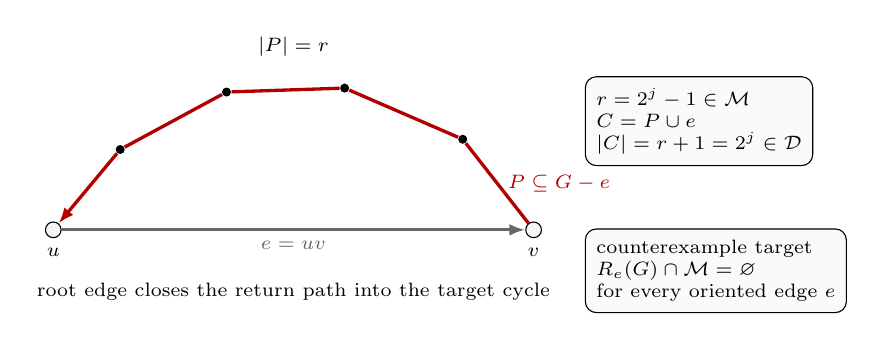
\begin{tikzpicture}[
vtx/.style={circle,draw,fill=black!4,inner sep=2pt},
mid/.style={circle,fill=black,inner sep=1.15pt},
root/.style={-{Latex[length=2mm]},very thick,black!60},
ret/.style={-{Latex[length=2mm]},very thick,red!70!black},
box/.style={rectangle,rounded corners,draw,align=left,inner sep=4pt,fill=black!2},
every node/.style={font=\scriptsize}
]
\node[vtx,label=below:$u$] (u) at (-3.05,0) {};
\node[vtx,label=below:$v$] (v) at (3.05,0) {};
\node[mid] (a) at (2.15,1.15) {};
\node[mid] (b) at (0.65,1.80) {};
\node[mid] (c) at (-0.85,1.75) {};
\node[mid] (d) at (-2.20,1.02) {};
\draw[root] (u)--node[below]{$e=uv$}(v);
\draw[ret] (v)--node[right]{$P\subseteq G-e$}(a)--(b)--(c)--(d)--(u);
\node[anchor=south] at (0,2.08) {$|P|=r$};
\node[box,anchor=west] at (3.70,1.38) {$r=2^j-1\in\Mers$\\
$C=P\cup e$\\
$|C|=r+1=2^j\in\Pow$};
\node[box,anchor=west] at (3.70,-0.52) {counterexample target\\
$R_e(G)\cap\Mers=\varnothing$\\
for every oriented edge $e$};
\node[anchor=north] at (0,-0.55) {root edge closes the return path into the target cycle};
\end{tikzpicture}%
}
\caption[Visual definition of a Mersenne return]{Visual definition of the edge-rooted target algebra.  The white circled vertices are the endpoints $u$ and $v$, the grey arrow is the oriented root edge $e=uv$, and the black dots are internal vertices of the return path.  The red path $P$ lies in $G-e$, runs from $v$ back to $u$, and has length $r=|P|$.  The box labelled $r=2^j-1\in\Mers$ records the target case: adjoining the root edge gives the simple cycle $C=P\cup e$ of length $|C|=r+1=2^j\in\Pow$.  The counterexample box records the equivalent local target condition $R_e(G)\cap\Mers=\varnothing$ for every oriented edge $e$.}
\label{fig:mersenne-return-gadget}
\end{figure}

\begin{lemma}[Two-path criterion]\label[lemma]{lem:two-path-criterion}
Let $P$ and $Q$ be internally vertex-disjoint simple paths with the same
endpoints.  Then $P\cup Q$ is a simple cycle of length $|P|+|Q|$.  In
particular, if $|P|+|Q|\in\Pow$, then $G$ contains a dyadic cycle.
\end{lemma}

\begin{proof}
The two paths meet only in their common endpoints, so traversing $P$ from one
endpoint to the other and then traversing $Q$ back gives a cycle with no
repeated internal vertex.  Its edge set is the disjoint union of the edge sets
of $P$ and $Q$, hence its length is $|P|+|Q|$.
\end{proof}

\begin{definition}[Counterexample]\label[definition]{def:counterexample}
A graph $G$ is a \emph{counterexample} if
\[
\delta(G)\ge3
\qquad\text{and}\qquad
R_e(G)\cap\Mers=\varnothing\quad\forall e\in\vec E(G).
\]
\end{definition}

\begin{definition}[Dyadic-safe; target-safe]\label[definition]{def:dyadic-safe}
A cycle is \emph{dyadic} if its length is a power of two.  A subgraph $X\subseteq G$ is \emph{dyadic-safe} (equivalently \emph{target-safe}) if $G$ contains no dyadic cycle meeting $V(X)$.  This is the contextual notion: such a cycle may run partly through $G-X$, so dyadic-safety of $X$ is a property of how $X$ is embedded in $G$, strictly stronger than the absence of a dyadic cycle internal to $X$.  For $X=G$ it is exactly the no-power-of-two-cycle clause of the counterexample condition.
\end{definition}

For contradiction, throughout the paper we assume that a counterexample exists and choose one, denoted $G$, lexicographically minimal by
\[
(|V(G)|,|E(G)|).
\]
Set
\[
n=|V(G)|,
\qquad
m=|E(G)|.
\]

\paragraph{Framework branch table.}
The target-cycle section supplies the first branch table.
\begin{longtable}{L{0.13\textwidth} L{0.19\textwidth} L{0.14\textwidth} L{0.14\textwidth} L{0.17\textwidth} L{0.17\textwidth}}
\FrameworkBranchTableHeader
Mersenne return
&
Some oriented edge \(e\) has \(R_e(G)\cap\Mers\ne\varnothing\).
&
No residual demand remains.
&
The root edge and return path.
&
One oriented edge.
&
Closed by \cref{lem:return-equivalence}.
\\
\addlinespace
Two-path closure
&
Two internally disjoint paths have dyadic total length.
&
No residual demand remains.
&
The two path lengths.
&
One unordered endpoint pair.
&
Closed by \cref{lem:two-path-criterion}.
\\
\addlinespace
Counterexample branch
&
All oriented edges avoid Mersenne returns.
&
The target-safe condition.
&
The counterexample definition.
&
Every oriented edge of \(G\).
&
This is the standing branch of \cref{def:counterexample}.
\\
\bottomrule
\end{longtable}

\section{Minimality and replacement}\label{sec:minimality-replacement}

\begin{lemma}[No proper core]\label[lemma]{lem:no-proper-core}
Every proper subgraph $H\subsetneq G$ satisfies $\delta(H)\le2$.
\end{lemma}

\begin{proof}
If $H\subsetneq G$ had $\delta(H)\ge3$, then $H$ would also have no power-of-two cycle, because every cycle of $H$ is a cycle of $G$.  Thus $H$ would be a smaller counterexample, contradicting the minimality of $G$.
\end{proof}

\begin{lemma}[Deletion criticality]\label[lemma]{lem:deletion-critical}
Every edge of $G$ has at least one endpoint of degree $3$.  In particular, the set $V_{\ge4}(G)$ is independent.
\end{lemma}

\begin{proof}
Suppose for contradiction that some edge $xy\in E(G)$ has $d_G(x),d_G(y)\ge4$.  Deleting $xy$ lowers the degrees of $x$ and $y$ by one, to at least $3$, and leaves every other degree unchanged, so $\delta(G-xy)\ge3$.  Moreover every cycle of $G-xy$ is a cycle of $G$, so deleting $xy$ creates no new cycle and in particular no new power-of-two cycle; hence $R_e(G-xy)\subseteq R_e(G)$ for every oriented edge $e$, and $G-xy$ has no power-of-two cycle.  Thus $G-xy$ is a counterexample with the same vertex set and one fewer edge, contradicting the edge-minimality of $G$.  Therefore no edge joins two vertices of degree at least $4$; equivalently, every edge has an endpoint of degree exactly $3$, and the set $V_{\ge4}(G)$ of vertices of degree at least $4$ is independent.
\end{proof}

\begin{lemma}[Sparse upper envelope]\label[lemma]{lem:sparse-upper-envelope}
The minimal counterexample satisfies
\[
m\le 2n-2.
\]
\end{lemma}

\begin{proof}
First \(G\) has at least one vertex of degree \(3\).  Otherwise every vertex
would have degree at least \(4\), and any edge of \(G\) would have two endpoints
of degree at least \(4\), contradicting \cref{lem:deletion-critical}.  Fix a
degree-\(3\) vertex \(v\).

Every subgraph of \(G-v\) is a proper subgraph of \(G\).  By
\cref{lem:no-proper-core}, each such subgraph has a vertex of degree at most
\(2\).  Hence \(G-v\) is \(2\)-degenerate.  A \(2\)-degenerate graph on
\(N\ge2\) vertices has at most \(2N-3\) edges: remove vertices in a degeneracy
order, count at most \(2\) deleted edges at each step until two vertices remain,
and then count at most one final edge.

Applying this with \(N=n-1\) gives
\[
e(G-v)\le 2(n-1)-3.
\]
Since \(d_G(v)=3\),
\[
m=e(G-v)+d_G(v)\le 2(n-1)-3+3=2n-2.
\]
\end{proof}

\begin{lemma}[Bridgelessness of the minimal counterexample]\label[lemma]{lem:bridgeless}
The graph $G$ has no bridge.  Consequently every edge of $G$ lies on a cycle; equivalently, $R_e(G)\ne\varnothing$ for every oriented edge $e\in\vec E(G)$.
\end{lemma}

\begin{proof}
Suppose for contradiction that $e=uv$ is a bridge.  Let $A$ and $B$ be the components of $G-e$ containing $u$ and $v$, respectively.  Form $G'$ from $G-e$ by identifying $u$ and $v$ to a single vertex $z$.

The graph $G'$ is simple.  Indeed, after deleting $e$, the neighbours of $u$ lie in $A-\{u\}$ and the neighbours of $v$ lie in $B-\{v\}$, which are disjoint.  Thus identifying $u$ and $v$ creates no parallel edge, and deleting $e$ before the identification creates no loop.

The minimum degree remains at least $3$.  Every vertex other than $z$ has the same degree as in $G$.  The identified vertex has
\[
d_{G'}(z)=d_G(u)+d_G(v)-2\ge4,
\]
since $d_G(u),d_G(v)\ge3$ and the bridge $uv$ is counted once at each endpoint before deletion.

Next, $G'$ has no power-of-two cycle.  Any cycle of $G'$ that uses $z$ and has vertices on both sides would contain, after deleting $z$, a path from a vertex of $A-\{u\}$ to a vertex of $B-\{v\}$ in $G'-z$.  This is impossible because $A-\{u\}$ and $B-\{v\}$ are disconnected in $G'-z$.  Hence every cycle of $G'$ lies wholly in the image of $A$ or wholly in the image of $B$, and is therefore already a cycle of $G$.  Since $G$ has no power-of-two cycle, neither does $G'$.

Thus $G'$ is a counterexample with $|V(G')|=|V(G)|-1$, contradicting the vertex-minimality of $G$.  Therefore $G$ has no bridge.  The final assertion follows because an edge is a bridge if and only if it lies on no cycle, and a cycle through an oriented edge $e=ab$ is exactly a return path from $b$ to $a$ in $G-e$ together with $e$.

For the finite formal audit, the contraction is represented without a graph
search: the name (v) is removed and every former (v)-edge other than
(uv) is reattached to (u).  The bridge condition makes the two endpoint
neighbourhoods disjoint.  They therefore inject into the new neighbourhood of
the identified vertex, while the neighbour set of every other vertex injects
under the same collapse map; this proves the minimum-degree assertion.  To
transport cycles, rotate a contracted cycle at the identified vertex.  Its
two incident cycle edges must both originate at (u) or both at (v), since
opposite origins would lift the cycle with its final edge removed to a
(u)--(v) walk in (G-uv).  Replacing the identified vertex by the common
origin then lifts the whole simple cycle injectively and preserves its length.
Thus the reduction uses a single supplied bridge and no enumeration of
components, paths, cycles, or graphs.
\end{proof}

\begin{lemma}[Cycle-rank pressure]\label[lemma]{lem:cycle-rank}
The cycle rank
\[
\beta(G)=m-n+1
\]
satisfies
\[
\beta(G)\ge \frac n2+1.
\]
\end{lemma}

\begin{proof}
Since $\delta(G)\ge3$, we have $2m=\sum_v d(v)\ge3n$.  Therefore $m-n+1\ge n/2+1$.
\end{proof}

\begin{definition}[Surplus ports and excess selectors]\label[definition]{def:surplus-ports}
Let
\[
H=V_{\ge4}(G).
\]
By Lemma~\ref{lem:deletion-critical}, $H$ is independent, so every neighbour of a vertex in $H$ has degree exactly $3$.

A \emph{surplus port} is an ordered edge
\[
p=(h,x)
\]
with $h\in H$ and $x\in N_G(h)$.  We write
\[
c(p)=h,\qquad x(p)=x
\]
for its high centre and cubic endpoint.  Since $d_G(x)=3$, there are two vertices, denoted $a_p,b_p$, such that
\[
N_G(x(p))=\{c(p),a_p,b_p\}.
\]
The unordered pair
\[
s(p)=\{a_p,b_p\}
\]
is the \emph{shoulder pair} of $p$, and the unordered pair
\[
e_p^*=a_pb_p
\]
is its \emph{shoulder chord}.

An \emph{excess selector} is a choice, for each $h\in H$, of a set
\[
\mathcal P_{\rm exc}(h)\subseteq \{(h,x):x\in N_G(h)\}
\]
of size $d_G(h)-3$.  We set
\[
\mathcal P_{\rm exc}=\bigcup_{h\in H}\mathcal P_{\rm exc}(h).
\]
Thus
\[
|\mathcal P_{\rm exc}|=\sum_{h\in H}(d_G(h)-3)=\sigma(G).
\]
The three unselected incident ports at a high vertex are its \emph{base ports}; the selected ports are exactly the units of degree surplus that one would like to remove in order to make the graph cubic.
\end{definition}

\begin{definition}[High centers and port types]\label[definition]{def:heavy-center-triangular-port}
A vertex $h\in V(G)$ is a \emph{high center} if $d_G(h)\ge4$, and a
\emph{heavy center} if $d_G(h)\ge5$.  Let
$p=(h,x)$ be a surplus port at a high center.  The port $p$ is
\emph{triangular} if its shoulder chord lies in \(G\):
\[
e_p^*\in E(G).
\]
Equivalently, if $N_G(x)=\{h,a_p,b_p\}$, then $x a_p b_p x$ is a triangle
not using $h$.  The port is \emph{open} if
\[
e_p^*\notin E(G).
\]
The word open records only the absence of the shoulder chord in \(G\); no
suppressed graph is associated to the port.
\end{definition}

\begin{remark}[Finite selected-port audit]\label[remark]{rem:finite-selected-port-audit}
Fix the declared vertex order and, at each center \(h\), take the first
\(d_G(h)-3\) neighbors as a canonical excess selector.  The local information
used below can then be exposed by five bounded scans followed by one
proof-level interpretation.  First, exclusion of a
cycle of length \(4\) gives the neighborhood matching and common-neighbor
conclusions of \cref{lem:heavy-neighbourhood-normal-form}.  Second, each
selected port is classified as open or triangular from the adjacency of its
two shoulder vertices.  Third, the open selected ports are grouped by their
center, producing either two at one center or the certificate that every
center contains at most one.  Fourth, only in the former branch, the two port
endpoints are compared over the declared vertex set by their adjacency
responses.  Finally, one local witness per selected port certifies its exact
two-shoulder contribution, so the resulting shoulder ledger has total
\(2|\mathcal P_{\rm exc}|\).  For the exact pair returned by the overloaded
center fibre, the four-cycle-free common-neighbor conclusion then proves that
nonadjacent endpoints have disjoint shoulder pairs and cannot occur in one
another's shoulder pair.  Thus this branch satisfies
\cref{def:fan-compatible-open-ports}; endpoint adjacency remains the explicit
complementary branch.  Finally, for any requested high center \(h\), one scan
of its declared neighbor schedule classifies all \(d_G(h)\) incident ports.
If the compatible-pair branch is absent, the matching-neighborhood conclusion
forces the open-port count to be at most two, and the exact open/triangular
cardinality partition gives at least \(d_G(h)-2\) triangular ports.  This is
the finite audit used in
\cref{lem:heavy-center-triangular-alternative,cor:heavy-center-local-dichotomy}.

These operations enumerate only the selected ports and the declared vertex
set.  In particular, they do not enumerate port pairs, vertex subsets,
completion graphs, or response tables.  In particular, the all-port step does
not construct the port-pair universe: the three-port contradiction in the
matching argument is proof-level.  This audit supplies local structural data;
it does not establish the Type B routing clauses, shoulder-completion routing,
or the free/blocked sparse pair-response assertions.
\end{remark}

\begin{lemma}[High-neighbourhood normal form]\label[lemma]{lem:heavy-neighbourhood-normal-form}
Let $h$ be a high center.  Then the following hold.
\begin{enumerate}[label=(\alph*), leftmargin=2.2em]
\item Every vertex in $N_G(h)$ has degree $3$.
\item The graph induced by $N_G(h)$ is a matching.
\item If $x,y\in N_G(h)$ are nonadjacent, then $x$ and $y$ have no common
neighbour outside $\{h\}$.
\end{enumerate}
\end{lemma}

\begin{proof}
For (a), apply \cref{lem:deletion-critical} to the edge $hx$.  Since
$d_G(h)\ge4$, the degree-$3$ endpoint of $hx$ is $x$.

For (b), suppose that $G[N_G(h)]$ contained two adjacent edges $xy$ and $yz$.
Then
\[
hxyzh
\]
is a simple cycle of length $4$, contradicting the assumption that $G$ contains
no power-of-two cycle.  Thus every vertex of $G[N_G(h)]$ has degree at most
$1$, so $G[N_G(h)]$ is a matching.

For (c), suppose that nonadjacent $x,y\in N_G(h)$ had a common neighbour
$z\ne h$.  Then
\[
hxzyh
\]
is a simple cycle of length $4$, again impossible.  Hence no such $z$ exists.
\end{proof}

\begin{definition}[Fan-compatible open ports]\label[definition]{def:fan-compatible-open-ports}
Let \(h\) be a high center, and let \(p=(h,x)\) and \(q=(h,y)\) be distinct
open ports at \(h\).  The pair \(\{p,q\}\) is \emph{fan-compatible} if
\[
x\notin s(q),\qquad y\notin s(p),\qquad s(p)\cap s(q)=\varnothing .
\]
Equivalently, the two shoulder pairs are disjoint and neither port vertex is a
shoulder endpoint for the other port; in this case the four non-\(h\)
incidences can be assigned as local Type B fan incidences.
\end{definition}

\begin{lemma}[Same-center open ports are fan-compatible]\label[lemma]{lem:same-center-open-port-compatibility}
Let \(h\) be a high center, and let \(p=(h,x)\) and \(q=(h,y)\) be distinct
open ports at \(h\).  If \(xy\notin E(G)\), then \(\{p,q\}\) is
fan-compatible.
\end{lemma}

\begin{proof}
Since \(xy\notin E(G)\), the endpoint \(x\) is not in the shoulder pair
\(s(q)\), and \(y\) is not in the shoulder pair \(s(p)\).  Suppose that
\(s(p)\cap s(q)\) contained a vertex \(z\).  Then \(z\ne h\), and the two
nonadjacent neighbours \(x,y\in N_G(h)\) would have the common neighbour \(z\)
outside \(\{h\}\).  This contradicts
\cref{lem:heavy-neighbourhood-normal-form}.  Hence the shoulder pairs are
disjoint, and the pair is fan-compatible by definition.
\end{proof}

\begin{lemma}[Heavy-center triangular alternative]\label[lemma]{lem:heavy-center-triangular-alternative}
Let $h$ be a heavy center of degree $k$.  If no two open ports at $h$ form a
fan-compatible open pair, then at least $k-2$ ports at $h$ are triangular.
In particular, at least three ports at $h$ are triangular.
\end{lemma}

\begin{proof}
Let $U\subseteq N_G(h)$ be the set of vertices $x$ such that the port $(h,x)$
is open.  If two vertices $x,y\in U$ were nonadjacent, then
\cref{lem:same-center-open-port-compatibility} would make the two ports
$(h,x)$ and $(h,y)$ fan-compatible, contrary to the hypothesis.  Therefore
every two vertices in $U$ are adjacent.

By \cref{lem:heavy-neighbourhood-normal-form}, $G[N_G(h)]$ is a matching.  A
matching has no clique of size $3$, so $|U|\le2$.  All ports at $h$ whose cubic
endpoint is not in $U$ are not open, hence triangular by
\cref{def:heavy-center-triangular-port}.  Therefore the number of triangular
ports at $h$ is at least
\[
k-|U|\ge k-2.
\]
Since $k\ge5$, this is at least $3$.
\end{proof}

\begin{corollary}[Heavy-center local dichotomy]\label[corollary]{cor:heavy-center-local-dichotomy}
Let $h$ be a heavy center.  Then one of the following alternatives holds.
\begin{enumerate}[label=(\roman*), leftmargin=2.2em]
\item There are two open ports at $h$ that are fan-compatible.
\item At least $d_G(h)-2$ ports at $h$ are triangular; in particular, $h$ has
three triangular ports.
\end{enumerate}
\end{corollary}

\begin{proof}
If the first alternative fails, then
\cref{lem:heavy-center-triangular-alternative} gives the second alternative.
\end{proof}

\begin{corollary}[Degree-four local activation]\label[corollary]{cor:degree-four-local-activation}
Let \(h\) be a high center with \(d_G(h)=4\).  Then one of the following
alternatives holds.
\begin{enumerate}[label=(\roman*), leftmargin=2.2em]
\item There are two open ports at \(h\) that are fan-compatible.
\item At least two ports at \(h\) are triangular.
\end{enumerate}
In case \textup{(i)}, any admissible Type B fan-window profile that records the
two ports and assigns their four non-\(h\) incidences routes through
\cref{cor:compatible-pair-typeB-routing}.  In case \textup{(ii)}, any
admissible Type B fan-window profile that records two triangular ports and
assigns their four triangle incidences routes through
\cref{prop:fan-closed-port-typeB-routing}; in the certificate-marked B1
survivor it has
\[
D_B(\mathfrak F_h)\ge2-\frac{11-4}{4}=\frac14>0 .
\]
\end{corollary}

\begin{proof}
Let \(U\subseteq N_G(h)\) be the set of vertices \(x\) such that the port
\((h,x)\) is open.  If two vertices \(x,y\in U\) are nonadjacent, then
\cref{lem:same-center-open-port-compatibility} gives a fan-compatible open
pair, which is alternative \textup{(i)}.  Suppose no such pair exists.  Then
every two vertices of \(U\) are adjacent.  By
\cref{lem:heavy-neighbourhood-normal-form}, the graph induced by \(N_G(h)\) is
a matching, so \(U\) has size at most \(2\).  Since \(d_G(h)=4\), at least
\(4-|U|\ge2\) ports at \(h\) are not open.  By
\cref{def:heavy-center-triangular-port}, those ports are triangular.  This is
alternative \textup{(ii)}.

The routing assertion in case \textup{(i)} is exactly
\cref{cor:compatible-pair-typeB-routing}, applied with \(k=4\).  In case
\textup{(ii)}, choose two triangular ports.  For each of them the two triangle
edges are precisely the two non-\(h\) incidences of the port vertex.  Once those
incidences are assigned to the fan envelope, both ports are fan-closed by
\cref{def:fan-closed-port}.  Applying
\cref{prop:fan-closed-port-typeB-routing} with \(r=2\) and \(k=4\) gives the
displayed deficit bound and the listed Type B alternatives.
\end{proof}

\begin{definition}[Triangular fan core and shoulder completions]\label[definition]{def:triangular-fan-core}
Let $h$ be a heavy center and let
\[
\mathcal T_h=\{p_i=(h,x_i):i\in I\}
\]
be a nonempty set of triangular ports at \(h\).  For each \(i\in I\), write
\[
N_G(x_i)=\{h,a_i,b_i\},\qquad S_i=\{a_i,b_i\},
\]
so that \(x_i a_i b_i x_i\) is a triangle.  The \emph{triangular fan core}
generated by \(\mathcal T_h\) is
\[
F_h(\mathcal T_h)
=
G\Big[\{h\}\cup\{x_i:i\in I\}\cup\bigcup_{i\in I}S_i\Big].
\]
The vertices in \(S_i\) are the \emph{shoulders} of \(p_i\).

Let \(s\in S_i\), and let \(s_i'\) denote the other vertex of \(S_i\).  A
\emph{shoulder-completion incidence} at \(s\) is an edge \(sy\in E(G)\) with
\[
y\notin\{x_i,s_i'\}.
\]
It is \emph{central} when \(y=h\), \emph{cross-triangular} when
\[
y\in\bigcup_{j\in I,\ j\ne i}S_j,
\]
and \emph{outside} when
\[
y\notin V(F_h(\mathcal T_h))\cup N_G(h).
\]
An outside incidence is the first edge by which the displayed triangular fan
core attaches to the rest of the graph.
\end{definition}

\begin{lemma}[Shoulder-completion bookkeeping]\label[lemma]{lem:triangular-shoulder-completion}
Let \(p_i=(h,x_i)\) be a triangular port at a heavy center \(h\), and let
\(S_i=\{a_i,b_i\}\).  Then the following hold.
\begin{enumerate}[label=(\alph*), leftmargin=2.2em]
\item Each shoulder \(s\in S_i\) has at least one shoulder-completion
incidence.
\item At most one shoulder in \(S_i\) lies in \(N_G(h)\).
\item If \(s\in S_i\cap N_G(h)\), then \(d_G(s)=3\), its unique
shoulder-completion incidence is the central edge \(sh\), and \(s\) has no
outside incidence.
\item No shoulder-completion incidence has endpoint in
\(N_G(h)\setminus\{h\}\).
\end{enumerate}
\end{lemma}

\begin{proof}
Fix \(s\in S_i\), and let \(s_i'\) be the other shoulder.  The two edges
\(sx_i\) and \(ss_i'\) are present.  Since \(\delta(G)\ge3\), \(s\) has at
least one incident edge different from these two; this proves (a).

If both \(a_i\) and \(b_i\) lay in \(N_G(h)\), then the vertex
\(x_i\in N_G(h)\) would be adjacent inside \(G[N_G(h)]\) to both \(a_i\) and
\(b_i\).  This contradicts the matching conclusion in
\cref{lem:heavy-neighbourhood-normal-form}.  Hence (b) holds.

Assume \(s\in N_G(h)\).  By \cref{lem:heavy-neighbourhood-normal-form},
\(d_G(s)=3\).  Its three neighbours are already \(h\), \(x_i\), and
\(s_i'\).  Thus the only shoulder-completion incidence at \(s\) is the central
edge \(sh\), proving (c).

Finally suppose that \(sy\) is a shoulder-completion incidence with
\(y\in N_G(h)\setminus\{h\}\).  If \(y\) were adjacent to \(x_i\), then
\(y\in S_i\), because the only neighbours of \(x_i\) are \(h,a_i,b_i\); this is
excluded by the definition of shoulder-completion incidence.  Hence \(x_i\) and
\(y\) are nonadjacent vertices of \(N_G(h)\).  They have the common neighbour
\(s\ne h\), contradicting
\cref{lem:heavy-neighbourhood-normal-form}.  This proves (d).

For the finite audit, the sites are the two shoulders of each actual
triangular port at the requested center, in the declared port and shoulder
order.  At one site the witness scan ranges only over the declared vertex
order and stops at the first endpoint satisfying the completion-incidence
predicate.  Thus there are at most \(2|V(G)|\) sites and at most
\(2|V(G)|^2+2|V(G)|+2\) primitive checks.  The audit constructs no path,
vertex subset, port pair, or auxiliary graph.
\end{proof}

\begin{lemma}[Port returns enter through shoulders]\label[lemma]{lem:triangular-port-return}
Let \(p_i=(h,x_i)\) be a triangular port at a heavy center \(h\).  Then there
is a shoulder \(s\in S_i\) and a simple \(s\)--\(h\) path \(Q\) in
\(G-x_i\).  Moreover, the cycle obtained from \(Q\) by adding the two edges
\[
hx_i,\qquad x_is
\]
has length \(|E(Q)|+2\), and therefore
\[
|E(Q)|\notin\{2^j-2:j\ge2\}.
\]
Exactly one of the following initial alternatives holds:
\begin{enumerate}[label=(\roman*), leftmargin=2.2em]
\item \(Q\) is the single central edge \(sh\);
\item the first edge of \(Q\) is a noncentral shoulder-completion incidence
at \(s\);
\item \(Q\) begins with the shoulder edge \(ss_i'\), followed by the central
edge \(s_i'h\), and has length \(2\);
\item \(Q\) begins with \(ss_i'\), followed by a noncentral
shoulder-completion incidence at \(s_i'\).
\end{enumerate}
\end{lemma}

\begin{proof}
By \cref{lem:bridgeless}, the edge \(hx_i\) lies on a cycle \(C\).  Deleting
\(hx_i\) from \(C\) gives a simple \(x_i\)--\(h\) path in \(G-hx_i\).  The first
edge of this path is \(x_is\) for some \(s\in S_i\).  Removing that first edge
leaves a simple \(s\)--\(h\) path \(Q\) in \(G-x_i\).

The edges of \(Q\), together with \(x_is\) and \(hx_i\), reconstruct the cycle
\(C\).  Since \(G\) has no power-of-two cycle, \(|E(Q)|+2\) is not a power of
two, which gives the displayed exclusion.

If the first edge of \(Q\) is \(sh\), simplicity forces \(Q=sh\), giving
(i).  Otherwise, if the first edge is not \(ss_i'\), its endpoint is neither
\(h\), \(x_i\), nor \(s_i'\), so it is a noncentral shoulder-completion
incidence at \(s\), giving (ii).  It remains to consider a first edge
\(ss_i'\).  The next edge exists because \(s_i'\ne h\).  It cannot return to
\(s\), because \(Q\) is simple, and it cannot go to \(x_i\), because
\(Q\subseteq G-x_i\).  If it is \(s_i'h\), simplicity again forces the path
to stop, giving (iii).  Every other possibility is a noncentral
shoulder-completion incidence at \(s_i'\), giving (iv).

The formal finite audit uses the non-bridge reachability theorem to obtain
one simple path in \(G-hx_i\) by proof-level choice.  CT1 checks the resulting
proof-carrying return certificate once.  The construction enumerates no
walks, paths, cycles, vertex subsets, subgraphs, or ambient graphs.
\end{proof}

\begin{lemma}[First landing exhaustion for triangular shoulders]\label[lemma]{lem:triangular-first-landing}
Let \(\mathcal T_h\) be a set of triangular ports at a heavy center \(h\).
Every shoulder-completion incidence in the triangular fan core
\(F_h(\mathcal T_h)\) is exactly one of the following:
\begin{enumerate}[label=(\roman*), leftmargin=2.2em]
\item a central incidence to \(h\);
\item a cross-triangular incidence to a shoulder of another port in
\(\mathcal T_h\);
\item an outside incidence with endpoint in
\[
V(G)\setminus\bigl(V(F_h(\mathcal T_h))\cup N_G(h)\bigr).
\]
\end{enumerate}
No completion incidence lands at another neighbour of \(h\), and no completion
incidence lands at another port vertex \(x_j\).
\end{lemma}

\begin{proof}
Let \(sy\) be a shoulder-completion incidence at a shoulder \(s\in S_i\).  If
\(y=h\), it is central.  If \(y\in N_G(h)\setminus\{h\}\), then
\cref{lem:triangular-shoulder-completion} forbids the incidence; in particular
this excludes \(y=x_j\) for every port vertex \(x_j\), because each
\(x_j\in N_G(h)\).

It remains that \(y\notin N_G(h)\).  If \(y\in V(F_h(\mathcal T_h))\), then
\(y\) cannot be \(h\), cannot be a port vertex \(x_j\), and cannot be
\(x_i\) or the other shoulder of \(p_i\) by the definition of completion
incidence.  Thus \(y\) is a shoulder of some other triangular port, and the
incidence is cross-triangular.  If \(y\notin V(F_h(\mathcal T_h))\), then it is
an outside incidence by definition.  These cases are disjoint and exhaustive.
\end{proof}

\begin{lemma}[Cross-shoulder multiplicity]\label[lemma]{lem:triangular-cross-shoulder}
Let \(p_i\) and \(p_j\) be distinct triangular ports at the same heavy center
\(h\).  If there are two distinct cross-triangular incidences between \(S_i\)
and \(S_j\), then either \(G\) contains a \(4\)-cycle or at least one shoulder
in \(S_i\cup S_j\) has ambient degree at least \(4\).  Consequently, after
routing high shoulders to the Type B surplus branch, the cross-triangular
incidences between any two shoulder pairs form a matching of size at most one.
\end{lemma}

\begin{proof}
Let the two cross-triangular edges be \(e_1\) and \(e_2\).  If they share a
shoulder endpoint \(s\), then \(s\) is incident with the two triangle edges
inside its own port and with both \(e_1\) and \(e_2\).  Hence \(d_G(s)\ge4\).

Assume therefore that \(e_1\) and \(e_2\) are vertex-disjoint.  Write
\(S_i=\{a_i,b_i\}\) and \(S_j=\{a_j,b_j\}\).  After relabelling the two
shoulders inside each pair, the cross edges are \(a_i a_j\) and \(b_i b_j\).
Then
\[
a_i a_j b_j b_i a_i
\]
is a simple cycle of length \(4\), using the cross edge \(a_i a_j\), the
triangular shoulder edge \(a_jb_j\), the cross edge \(b_jb_i\), and the
triangular shoulder edge \(b_ia_i\).  This contradicts dyadic-safety unless the
high-shoulder alternative already occurred in the shared-endpoint case.

If all shoulders have ambient degree \(3\), the shared-endpoint case is
impossible and the vertex-disjoint case gives a forbidden \(4\)-cycle.  Thus at
most one cross-triangular edge can join \(S_i\) to \(S_j\), and the remaining
incidences form a matching.
\end{proof}

\begin{remark}[Degree-greater-than-four residual leaf]\label[remark]{rem:degree-greater-four-leaf}
\Cref{cor:heavy-center-local-dichotomy} isolates the degree-greater-than-four
branch into two local configurations.  In Leaf A, a fan-compatible open pair is
recorded as two fan-closed ports by
\cref{lem:compatible-pair-fan-closure}; \cref{cor:compatible-pair-typeB-routing}
then gives a positive-deficit Type B fan whenever the fan is
certificate-marked and survives the direct target, compression, and
delocalization alternatives.  If one of those direct alternatives occurs, the
branch is already closed; if the fan is unmarked or the local entries cannot be
globally disjoint, the branch is recorded as a fan-certificate residual center
or a B2-overlap obstruction.  In Leaf B, the
triangular branch is routed by
\cref{def:triangular-fan-core,lem:triangular-shoulder-completion,lem:triangular-first-landing,lem:triangular-cross-shoulder}
and by the Type B fan ledger in
\cref{prop:triangular-port-typeB-routing}: the guaranteed triangular ports are
cubic-closed fan neighbours, their shoulder-completion incidences have only the
central, cross-triangular, and outside first landings listed above, and the
cross-triangular multiplicity left after high-shoulder routing is a matching
survivor.  The common primitive in both leaves is fan-closedness: two assigned
non-\(h\) incidences at a cubic neighbour of \(h\) contribute one
cubic-closed fan neighbour.  Thus any heavy center of degree \(k\ge5\) supplies
at least two fan-closed ports after the local dichotomy, and
\cref{prop:fan-closed-port-typeB-routing} gives
\[
D_B\ge 2-\frac{11-k}{4}=\frac{k-3}{4}>0 .
\]
Thus the active degree-greater-than-four closure is the Type B fan-closed
ledger.
\end{remark}

\begin{remark}[Interface with the surplus-token branch]\label[remark]{rem:near-cubic-remaining-packing}
\Cref{cor:heavy-center-local-dichotomy} separates the degree-greater-than-four
branch from the degree-$4$ branch.  The degree-greater-than-four branch is
routed through fan-closed Type B data by
\cref{cor:compatible-pair-typeB-routing,prop:triangular-port-typeB-routing}.
This local dichotomy is one input to the sparse surplus-token branch, not a
replacement for it.  Excess ports that do not close through the direct target,
compression, delocalization, or fan-closed Type B alternatives are counted by
the active surplus family \(\mathcal P_{\rm exc}\).  The non-near-cubic branch
then applies the free/blocked pair split and the capacity-token ledger of
\cref{def:capacity-token-ledger}.  Consequently any attempted survivor above
the near-cubic range first produces one of the three role-homogeneous
same-token audit classes of
\cref{def:same-token-blocker-roles,cor:forced-homogeneous-same-token-scale}:
window-incidence, remainder-surplus, or primitive-carrier load, with a fixed
blocker type and token subtype.  The same-token bottleneck routing of
\cref{lem:same-token-bottleneck-routing} then either realizes a sparse surplus
exit, produces ordinary Type B fan data, or leaves fixed homogeneous caps and
hence the near-cubic estimate.
\end{remark}

\begin{definition}[Open-port suppression]\label[definition]{def:open-port-suppression}
Let \(p=(h,x)\) be an open surplus port, so
\[
N_G(x)=\{h,a_p,b_p\},\qquad a_pb_p\notin E(G).
\]
The \emph{suppression} of \(p\) is the graph
\[
G/p := G-x+a_pb_p .
\]

A finite family \(\mathcal Q\) of open surplus ports is
\emph{suppressible} if the following four conditions hold.
\begin{enumerate}[label=(\alph*), leftmargin=2.2em]
\item The non-center supports
\[
T(p)=\{x(p),a_p,b_p\}\qquad (p\in\mathcal Q)
\]
are pairwise disjoint.
\item No selected center is contained in any non-center support:
\[
\{c(p):p\in\mathcal Q\}\cap\bigcup_{p\in\mathcal Q}T(p)=\varnothing .
\]
\item The shoulder chords \(e_p^*=a_pb_p\), \(p\in\mathcal Q\), are pairwise
distinct and none is an edge of \(G\).
\item For every high center \(h\),
\[
|\{p\in\mathcal Q:c(p)=h\}|\le d_G(h)-3 .
\]
\end{enumerate}
For a suppressible family \(\mathcal Q\), define
\[
G/\mathcal Q
=
G-\{x(p):p\in\mathcal Q\}
+\{a_pb_p:p\in\mathcal Q\}.
\]
Thus \(G/\{p\}=G/p\).
\end{definition}

\begin{lemma}[Suppression preserves simplicity and minimum degree]\label[lemma]{lem:open-port-suppression-safe}
If \(\mathcal Q\) is a suppressible family of open surplus ports, then
\(G/\mathcal Q\) is finite and simple, and every vertex of \(G/\mathcal Q\)
has degree at least \(3\).
\end{lemma}

\begin{proof}
Only the vertices \(x(p)\), \(p\in\mathcal Q\), are deleted, so the resulting
graph is finite.  No added edge is a loop, because \(a_p\ne b_p\).  No added
edge duplicates an old edge, and no two added edges duplicate each other, by
the definition of a suppressible family.  Hence \(G/\mathcal Q\) is simple.

Let \(v\) be a vertex that remains after the suppression.  If \(v=c(p)\) for
some selected ports, then the only deleted neighbours of \(v\) are the port
vertices \(x(p)\) with center \(v\): condition (b) prevents \(v\) from lying in
any other selected non-center support.  Thus
\[
d_{G/\mathcal Q}(v)
=
d_G(v)-|\{p\in\mathcal Q:c(p)=v\}|
\ge d_G(v)-(d_G(v)-3)=3
\]
by condition (d).

If \(v\) is a shoulder endpoint for a selected port \(p\), then condition (a)
makes this selected port unique.  The vertex \(v\) loses the edge \(vx(p)\) and
gains exactly the shoulder chord \(e_p^*\).  It is not deleted and is not a
selected center by condition (b).  Hence its degree is unchanged.  Every other
remaining vertex loses no incident edge and gains no incident edge, or only
gains an added chord.  Since \(\delta(G)\ge3\), all remaining vertices have
degree at least \(3\).
\end{proof}

\begin{lemma}[Single-port suppression witness]\label[lemma]{lem:single-open-port-suppression-witness}
Let \(G\) be the lexicographically minimal counterexample, and let \(p=(h,x)\)
be an open surplus port.  Then \(G-x\) contains a simple \(a_p\)--\(b_p\) path
of length \(2^j-1\) for some \(j\ge2\).
\end{lemma}

\begin{proof}
The singleton \(\{p\}\) is suppressible.  By
\cref{lem:open-port-suppression-safe}, \(G/p\) is a finite simple graph with
minimum degree at least \(3\).  It has one fewer vertex than \(G\).  By the
minimality of \(G\), the graph \(G/p\) contains a cycle \(C\) of length \(2^j\)
for some \(j\ge2\).

The cycle \(C\) must use the added shoulder chord \(a_pb_p\).  Otherwise all
edges of \(C\) are old edges of \(G\) not incident with the deleted vertex
\(x\), and \(C\) is already a power-of-two cycle in \(G\), impossible.  Deleting
the chord \(a_pb_p\) from \(C\) leaves a simple \(a_p\)--\(b_p\) path in
\(G-x\), and its length is \(2^j-1\).
\end{proof}

\begin{lemma}[Suppressed-family critical cycle]\label[lemma]{lem:suppressed-family-critical-cycle}
Let \(G\) be the lexicographically minimal counterexample, and let
\(\varnothing\ne\mathcal Q\) be a suppressible family of open surplus ports.
Then \(G/\mathcal Q\) contains a power-of-two cycle using at least one added
shoulder chord.  If a power-of-two cycle \(C\) in \(G/\mathcal Q\) has length
\(2^j\) and uses exactly the added chords indexed by
\(\mathcal S\subseteq\mathcal Q\), then \(\mathcal S\ne\varnothing\), and
replacing each added chord \(a_pb_p\) with the two-edge path
\[
a_p x(p) b_p
\]
gives a simple cycle of \(G\) of length \(2^j+|\mathcal S|\).  Consequently
\[
2^j+|\mathcal S|
\]
is not a power of two.
\end{lemma}

\begin{proof}
By \cref{lem:open-port-suppression-safe}, \(G/\mathcal Q\) is finite, simple,
and has minimum degree at least \(3\).  Since \(\mathcal Q\ne\varnothing\), it
has fewer vertices than \(G\).  Minimality gives a cycle \(C\) in
\(G/\mathcal Q\) whose length is a power of two.  If \(C\) used no added
shoulder chord, then \(C\) would be a power-of-two cycle already present in
\(G\), a contradiction.  Hence the set \(\mathcal S\) of added chords used by
\(C\) is nonempty.

For each \(p\in\mathcal S\), replace the edge \(a_pb_p\) on \(C\) by the path
\(a_p x(p)b_p\).  The supports \(T(p)\) are pairwise disjoint, and none of the
vertices \(x(p)\) is present in \(G/\mathcal Q\).  Therefore these replacements
are internally disjoint and introduce no repeated vertex.  The resulting closed
walk is a simple cycle in \(G\).  Each replacement adds exactly one edge, so the
new length is \(2^j+|\mathcal S|\).  Since \(G\) has no power-of-two cycle, this
integer is not a power of two.
\end{proof}

\begin{lemma}[Sparse slack identity]\label[lemma]{lem:sparse-slack-surplus}
For the standing parameters
\[
\lambda=2n-3-m,\qquad \sigma(G)=2m-3n,
\]
one has
\[
\sigma(G)=n-6-2\lambda
\qquad\text{and}\qquad
m=\frac32n+\frac12\sigma(G).
\]
Thus every additional unit of high-degree surplus consumes exactly one half-unit
of the sparse slack \(\lambda\).
\end{lemma}

\begin{proof}
Substituting \(m=2n-3-\lambda\) gives
\[
2m-3n=2(2n-3-\lambda)-3n=n-6-2\lambda.
\]
The second identity is the same equality solved for \(m\).
\end{proof}

\begin{definition}[Sparse surplus exits]\label[definition]{def:named-surplus-exits}
A \emph{sparse surplus exit} is one of the following conclusions, each of which
is defined without invoking the near-cubic Type A/Type B branch machinery:
\begin{enumerate}[label=(\alph*), leftmargin=2.2em]
\item a direct dyadic contradiction, equivalently a power-of-two cycle or a
Mersenne return in the sense of \cref{lem:return-equivalence};
\item a target-defective quotient, as defined by
\cref{lem:context-universality};
\item a nontrivial target-complete compression of a proper atom, forbidden by
\cref{lem:replacement,cor:uncompressible};
\item a proper or global delocalization coordinate governed by
\cref{lem:proper-smearing,lem:no-silent-global-smearing};
\item an open-port suppression cycle whose chord set violates the arithmetic
conclusion of \cref{lem:suppressed-family-critical-cycle}.
\end{enumerate}
A graph \emph{survives the sparse surplus exits} when none of these conclusions
occurs for any selected surplus demand, any selected pair of surplus demands,
or any baseline spine coordinate used in the entropy sandwich of
\cref{def:baseline-spine-demand}.
The label name \texttt{def:named-surplus-exits} is retained for references in
the dependency diagram; the exits in this branch are precisely the sparse exits
listed above.
\end{definition}

\begin{lemma}[Excess-port extraction]\label[lemma]{lem:sparse-excess-port-extraction}
Let \(G\) be the lexicographically minimal counterexample, and let
\(\mathcal P_{\rm exc}\) be the excess selector of
\cref{def:surplus-ports}.  Then
\[
|\mathcal P_{\rm exc}|=\sigma(G).
\]
Moreover, for every \(p=(h,x)\in\mathcal P_{\rm exc}\), the vertex \(h\) has
degree at least \(4\), the vertex \(x\) has degree \(3\), and
\[
N_G(x)=\{h,a_p,b_p\}
\]
for two distinct vertices \(a_p,b_p\ne h\).
\end{lemma}

\begin{proof}
By definition, each high-degree vertex \(h\) contributes exactly
\(d_G(h)-3\) selected incident ports to \(\mathcal P_{\rm exc}\).  The
high-degree vertices are precisely the vertices contributing positive terms to
\(\sigma(G)=\sum_v(d_G(v)-3)\), because every vertex of \(G\) has degree at
least \(3\).  Hence
\[
|\mathcal P_{\rm exc}|
=\sum_{h\in V_{\ge4}(G)}(d_G(h)-3)
=\sigma(G).
\]
If \(p=(h,x)\) is a selected port, then \(h\in V_{\ge4}(G)\).  By
\cref{lem:deletion-critical}, every edge has at least one degree-\(3\)
endpoint and \(V_{\ge4}(G)\) is independent.  Since \(h\) is not degree \(3\),
the other endpoint \(x\) must have degree \(3\).  Thus \(x\) has exactly two
neighbours different from \(h\), denoted \(a_p\) and \(b_p\).
\end{proof}

\begin{remark}[Ordered CT6 audit]\label{rem:ordered-surplus-ct6}
The finite audit underlying the extraction is performed in the declared
vertex order.  At a vertex \(h\), the monitored failure is
\[
d_G(h)\ge4
\quad\text{and}\quad
\exists x\in N_G(h)\text{ with }d_G(x)\ne3.
\]
The first-failure branch retains the first such centre.  If no failure is
found, the active ledger assigns contribution \(d_G(h)-3\) to \(h\), so its
total is exactly
\[
\sum_{h\in V(G)}(d_G(h)-3)=\sigma(G).
\]
The dependent slot family
\(\{(h,i):0\le i<d_G(h)-3\}\) has the same cardinality.  Deletion
criticality excludes the failure branch: on an edge \(hx\) with
\(d_G(h)\ge4\), the degree-three endpoint must be \(x\).  Thus this audit
uses one bounded neighbour scan per vertex, hence at most quadratic primitive
adjacency/degree tests, and does not enumerate paths, subgraphs, or graphs.
The return and suppression paths in
\cref{lem:sparse-port-activation} are supplied separately by bridgelessness
and minimality; the baseline demand of node~[129] is fixed only after this
activation stage.
\end{remark}

\begin{lemma}[Sparse port activation]\label[lemma]{lem:sparse-port-activation}
For every selected port \(p=(h,x)\in\mathcal P_{\rm exc}\), fix a
proof-carrying finite response support \(\Gamma(p)\) with the following
properties.
\begin{enumerate}[label=(\alph*), leftmargin=2.2em]
\item The port support is \(T(p)=\{x,a_p,b_p\}\).
\item There is a simple \(x\)--\(h\) path \(R_p\subseteq G-hx\).  Its first
edge after \(x\) is either \(xa_p\) or \(xb_p\).
\item If \(p\) is open, let \(Q_p\subseteq G-x\) be one fixed path supplied by
\cref{lem:single-open-port-suppression-witness}; this path joins \(a_p\) to
\(b_p\) and has length \(2^{j(p)}-1\) for some \(j(p)\ge2\).
\item The response support is the exact edge-labelled subgraph
\[
 E(\Gamma(p))=
 \begin{cases}
 E(R_p)\cup E(Q_p)\cup\{xa_p,xb_p\},&p\text{ open},\\
 E(R_p)\cup\{xa_p,xb_p,a_pb_p\},&p\text{ triangular},
 \end{cases}
\]
with vertex set consisting exactly of the endpoints of these edges.  Thus in
the triangular case the second summand is exactly the response triangle
\(xa_pb_px\), not an unspecified supergraph of it.
\end{enumerate}
The witnesses \(R_p,Q_p\) are fixed once for each selected port.  Every later
local scan consumes these declared certificates and checks their edge lists;
it does not search a path family.
\end{lemma}

\begin{proof}
By \cref{lem:bridgeless}, the edge \(hx\) is not a bridge.  Therefore \(h\) and
\(x\) remain connected in \(G-hx\), and there is a simple \(x\)--\(h\) path in
\(G-hx\).  Fix one such path and call it \(R_p\).
Since \(d_G(x)=3\) and \(N_G(x)=\{h,a_p,b_p\}\), the first edge of \(R_p\) after
\(x\) is one of \(xa_p,xb_p\).

If \(p\) is open, \cref{lem:single-open-port-suppression-witness} supplies a
simple \(a_p\)--\(b_p\) path \(Q_p\subseteq G-x\) of length \(2^{j(p)}-1\);
fix one such certificate.  If \(p\) is triangular, then
\(a_pb_p\in E(G)\), so \(xa_pb_px\) is a triangle.  In the open case take the
displayed union of \(R_p,Q_p\), and the two shoulder incidences; in the
triangular case take the displayed union of \(R_p\) and the three triangle
edges.  Both unions are connected and finite, contain \(T(p)\), and their edge
and vertex sets are fixed by the display.  Once the proof-carrying paths are
fixed, the display determines \(\Gamma(p)\) exactly.
\end{proof}

\begin{definition}[Active surplus demands]\label[definition]{def:active-surplus-demands}
Let \(G\) be a lexicographically minimal counterexample reaching node \([18]\).
An \emph{active surplus demand} is a selected surplus port
\[
p=(h,x)\in\mathcal P_{\rm exc}
\]
equipped with the fixed declared data \(T(p)\), \(R_p\), and \(\Gamma(p)\) from
\cref{lem:sparse-port-activation}, and not already removed by a sparse surplus
exit of \cref{def:named-surplus-exits}.  The response support \(\Gamma(p)\) is
used only as a carrier of target-response data; no disjointness between
distinct response supports is assumed unless it is explicitly stated.
\end{definition}

\begin{lemma}[Surviving active family is the full excess-port family]\label[lemma]{lem:surviving-active-family}
If \(G\) survives the sparse surplus exits, then
\[
\mathcal A_0:=\mathcal P_{\rm exc}
\]
is a finite family of active surplus demands and
\[
|\mathcal A_0|=\sigma(G).
\]
\end{lemma}

\begin{proof}
By \cref{lem:sparse-excess-port-extraction}, every selected port
\(p\in\mathcal P_{\rm exc}\) has the canonical data \(T(p)\), \(R_p\), and
\(\Gamma(p)\) supplied by \cref{lem:sparse-port-activation}.  Since \(G\)
survives the sparse surplus exits, no selected surplus demand is removed by an
exit of \cref{def:named-surplus-exits}.  Thus every \(p\in\mathcal P_{\rm exc}\)
is active in the sense of \cref{def:active-surplus-demands}.  The cardinality is
exactly \(|\mathcal P_{\rm exc}|=\sigma(G)\), again by
\cref{lem:sparse-excess-port-extraction}.
\end{proof}

\begin{definition}[Canonical local connector support]\label[definition]{def:sparse-canonical-connector}
For two nonempty connected finite edge-labelled subgraphs \(A,B\subseteq G\),
run multi-source breadth-first search from \(V(A)\) until \(V(B)\) is reached.
Among the endpoint pairs at minimum distance choose the lexicographically first
pair, and among their shortest paths choose the lexicographically first
predecessor path \(P_G(A,B)\).  Define
\[
J_G(A,B):=A\cup P_G(A,B)\cup B.
\]
If \(A\cap B\ne\varnothing\), this path has length zero at the least common
vertex.  For an unordered active pair \(\pi=\{p,q\}\), first order \(p<q\) in
the selected-port order and put
\[
X_\pi:=J_G(\Gamma(p),\Gamma(q)).
\]
Thus \(X_\pi\) is a specified connected support, not a minimum Steiner
subgraph.  It is computed by one multi-source BFS and one predecessor trace,
and checking it does not enumerate connected subgraphs or paths.
\end{definition}

\begin{definition}[Sparse surplus blockers]\label[definition]{def:surplus-blockers}
Let \(\mathcal A_0\) be a finite family of active surplus demands.  A
\emph{sparse surplus blocker} for an unordered pair
\(\pi=\{p,q\}\subseteq\mathcal A_0\) is a tagged value \(B=(\tau,b)\), where
\[
\tau\in\mathsf{BlkTag}:=\{\mathsf{overlap},\mathsf{return},
\mathsf{shoulder},\mathsf{profile},\mathsf{target},\mathsf{chord}\},
\]
and \(b\) is one of the following concrete finite values of the indicated tag.
\begin{enumerate}[label=(\alph*), leftmargin=2.2em]
\item For \(\tau=\mathsf{overlap}\), \(b\) is a vertex or edge-incidence
contained in both exact demand supports
\[
\Gamma(p)\cap\Gamma(q).
\]
\item For \(\tau=\mathsf{return}\), \(b\) is a common vertex or common
edge-incidence of the two canonical return paths \(R_p\) and \(R_q\).
\item For \(\tau=\mathsf{shoulder}\), \(b\) is a vertex in
\[
\{a_p,b_p,x(p)\}\cap\{a_q,b_q,x(q)\},
\]
together with its two role labels in
\(\{\mathsf{leftShoulder},\mathsf{rightShoulder},\mathsf{buffer}\}\).
\item For \(\tau=\mathsf{profile}\), \(b=(\xi,v)\), where \(\xi\) is a
boundary-degree-profile coordinate in the declared exact signature on
\(X_\pi\), \(v\) is its value in the labelled pair state, and this entry
prevents the proposed quotient or replacement from staying in a single fibre,
in the sense of
\cref{lem:degree-profile-fibres};
\item For \(\tau=\mathsf{target}\), \(b=(\xi,v)\), where \(\xi\) is a
target-response coordinate in the declared exact signature on \(X_\pi\),
\(v\) is its exact finite response-table value, and the entry witnesses a
target-defective quotient, target-complete compression, or delocalization
event, in the sense of
\cref{lem:context-universality,cor:uncompressible,lem:proper-smearing,lem:no-silent-global-smearing};
\item For \(\tau=\mathsf{chord}\), \(b=(\mathcal Q,C,\mathcal S)\), where
\(\varnothing\ne\mathcal Q\subseteq\{p,q\}\) is suppressible, \(C\) is a
proof-carrying simple power-of-two cycle in \(G/\mathcal Q\), and
\(\varnothing\ne\mathcal S\subseteq\mathcal Q\) is exactly the set of added
shoulder chords used by \(C\), as in
\cref{lem:suppressed-family-critical-cycle}.
\end{enumerate}
The blocker must be an object explicitly listed above.  A pair is not declared
blocked merely because the proof has not found a closure; its failed
compatibility must be represented by a finite-capacity object of one of these
six types.
\end{definition}

\begin{lemma}[Sparse blocker values are finite]\label[lemma]{lem:sparse-blocker-values-finite}
For every active pair \(\pi\), the tagged carrier
\(\mathsf{Blk}(\pi)\) of \cref{def:surplus-blockers} is finite.  A proposed
member is checked from \(X_\pi\), the two exact response supports, and, only in
the chord case, the supplied cycle certificate; checking membership does not
enumerate ambient subgraphs or paths.
\end{lemma}

\begin{proof}
The carriers in (a)--(c) are subsets of finite supports.  The exact signature
of the finite boundaried support \(X_\pi\) has finitely many coordinate labels,
each with a finite value type, so (d) and (e) are finite.  In (f) there are only
three nonempty choices for \(\mathcal Q\subseteq\{p,q\}\); a finite graph has
finitely many simple cycles, and each cycle determines \(\mathcal S\) by
inspection.  The verifier need not generate those cycles: the tuple contains
\(C\), and simplicity, length, and the used-chord set are checked by one scan
of its supplied edge list.
\end{proof}

\begin{definition}[Canonical sparse-blocker order]\label[definition]{def:canonical-sparse-blocker-order}
Fix the vertex order used in the lexicographic choices above.  Sparse surplus
blockers are ordered as follows.  First order by the type number
(a)--(f) in \cref{def:surplus-blockers}.  Within a type, order vertices by the
fixed vertex order, edge-incidences lexicographically by their ordered endpoint
pair and incident end, boundary-profile and target-response coordinates by the
lexicographic order of their declared labels, finite values, and supports, and
chord tuples by the lexicographic order of
\((\mathcal Q,E(C),\mathcal S)\).
This gives a total order on every finite set of blockers arising from a fixed
pair of active surplus demands.
\end{definition}

\begin{definition}[Canonical blocker ledger]\label[definition]{def:canonical-blocker-ledger}
Let \(\mathcal A_0\) be a finite family of active surplus demands and put
\[
\Pi(\mathcal A_0)=\binom{\mathcal A_0}{2}.
\]
For \(\pi=\{p,q\}\in\Pi(\mathcal A_0)\), let
\(\mathsf{Blk}(\pi)\) be the finite set of sparse surplus blockers for
\(\pi\) in the sense of \cref{def:surplus-blockers}.  Define
\[
\Pi_{\rm blk}:=\{\pi\in\Pi(\mathcal A_0):\mathsf{Blk}(\pi)\ne\varnothing\},
\qquad
\Pi_{\rm free}:=\Pi(\mathcal A_0)\setminus\Pi_{\rm blk}.
\]
For every \(\pi\in\Pi_{\rm blk}\), the \emph{canonical blocker} is
\[
\Phi_{\rm can}(\pi):=\min_{\prec}\mathsf{Blk}(\pi),
\]
where \(\prec\) is the order of \cref{def:canonical-sparse-blocker-order}.  The
canonical blocker set and incidence ledger are
\[
\mathcal B_{\rm can}:=\Phi_{\rm can}(\Pi_{\rm blk}),\qquad
\mathfrak I_{\rm can}:=
\{(\pi,\Phi_{\rm can}(\pi)):\pi\in\Pi_{\rm blk}\}.
\]
For \(B\in\mathcal B_{\rm can}\), write
\[
\mu(B):=|\Phi_{\rm can}^{-1}(B)|.
\]
\end{definition}

\begin{lemma}[Canonical blocker ledger has no overcounting]\label[lemma]{lem:canonical-blocker-ledger-no-overcount}
For every finite family \(\mathcal A_0\) of active surplus demands,
\[
|\Pi_{\rm blk}|=|\mathfrak I_{\rm can}|
=\sum_{B\in\mathcal B_{\rm can}}\mu(B).
\]
Consequently, if \(\mu(B)\le M\) for every \(B\in\mathcal B_{\rm can}\) and
\(|\mathcal B_{\rm can}|\le C_B n\), then
\[
|\Pi_{\rm blk}|\le MC_B n .
\]
\end{lemma}

\begin{proof}
The map
\[
\pi\longmapsto(\pi,\Phi_{\rm can}(\pi))
\]
is a bijection from \(\Pi_{\rm blk}\) to \(\mathfrak I_{\rm can}\), so
\(|\Pi_{\rm blk}|=|\mathfrak I_{\rm can}|\).  The fibres
\(\Phi_{\rm can}^{-1}(B)\), \(B\in\mathcal B_{\rm can}\), form a disjoint
partition of \(\Pi_{\rm blk}\).  Hence
\[
|\Pi_{\rm blk}|=\sum_{B\in\mathcal B_{\rm can}}|\Phi_{\rm can}^{-1}(B)|
=\sum_{B\in\mathcal B_{\rm can}}\mu(B).
\]
The displayed upper bound follows by applying \(\mu(B)\le M\) to each summand
and then using \(|\mathcal B_{\rm can}|\le C_B n\).
\end{proof}

\begin{definition}[Primitive carrier of a sparse blocker]\label[definition]{def:primitive-sparse-blocker-carrier}
An \emph{edge-incidence} of \(G\) is an ordered pair \((e,v)\) with
\(e\in E(G)\) and \(v\in e\).  The primitive sparse carrier universe is
\[
\mathfrak U_{\rm sp}(G):=
V(G)\sqcup I_E(G)\sqcup\mathcal P_{\rm exc},
\qquad
I_E(G):=\{(e,v):e\in E(G),\,v\in e\}.
\]
Each sparse surplus blocker \(B\) has a primitive carrier
\[
\kappa(B)\in\mathfrak U_{\rm sp}(G)
\]
defined as follows.
\begin{enumerate}[label=(\alph*), leftmargin=2.2em]
\item If \(B=(\mathsf{overlap},b)\), where \(b\) is its vertex or
edge-incidence value, then \(\kappa(B)=b\).
\item If \(B=(\mathsf{return},b)\), where \(b\) is its vertex or
edge-incidence value, then \(\kappa(B)=b\).
\item If \(B=(\mathsf{shoulder},(v,\ell_p,\ell_q))\), then
\(\kappa(B)=v\); the finite role labels remain part of the blocker value.
\item If \(B=(\mathsf{profile},(\xi,v))\) or
\(B=(\mathsf{target},(\xi,v))\), then \(\kappa(B)\) is the least vertex,
edge-incidence, or selected surplus port contained in the declared support of
\(\xi\).  The finite value \(v\) is retained in the blocker value but does not
alter its carrier.  Paths and windows contribute their least contained vertex
or edge-incidence.  This carrier exists because every sparse pair-response
coordinate is supported on \(X_\pi\supseteq\Gamma(p)\cup\Gamma(q)\), and the
declared signature of
\cref{def:declared-coordinate-signature} generates quotient coordinates only
from finite unions of declared supports.
\item If \(B=(\mathsf{chord},(\mathcal Q,C,\mathcal S))\), then
\(\kappa(B)\) is the least selected surplus port whose shoulder chord belongs to
\(\mathcal S\).  The set \(\mathcal S\) is nonempty by
\cref{lem:suppressed-family-critical-cycle}.
\end{enumerate}
All minima use the fixed vertex order, the induced lexicographic order on
edge-incidences, and the selected-port order used in
\cref{def:canonical-sparse-blocker-order}.
\end{definition}

\begin{lemma}[Primitive carrier supply is linear]\label[lemma]{lem:primitive-carrier-supply}
For every lexicographically minimal counterexample reaching the sparse-surplus
branch,
\[
|\mathfrak U_{\rm sp}(G)|\le 6n .
\]
\end{lemma}

\begin{proof}
\[
|\mathfrak U_{\rm sp}(G)|
=|V(G)|+|I_E(G)|+|\mathcal P_{\rm exc}|
=n+2m+\sigma(G).
\]
By \cref{lem:sparse-upper-envelope}, \(m\le2n-2\), so \(2m\le4n-4\).  Also
\[
\sigma(G)=2m-3n\le n-4\le n,
\]
again using \(m\le2n-2\).  Hence
\[
|\mathfrak U_{\rm sp}(G)|\le n+(4n-4)+n\le6n .
\]
\end{proof}

\begin{definition}[Capacity tokens for blocked surplus pairs]\label[definition]{def:capacity-token-ledger}
The \emph{capacity-token universe} is the disjoint union
\[
\mathfrak T_{\rm cap}
=
\mathfrak T_{\rm prim}\sqcup\mathfrak T_R\sqcup\mathfrak T_W,
\]
defined as follows.
\[
\mathfrak T_{\rm prim}:=\mathfrak U_{\rm sp}(G).
\]
The remainder-surplus tokens are
\[
\mathfrak T_R
:=
\{(v,j):v\in R,\ 1\le j\le d_G(v)-3\}.
\]
Thus \(|\mathfrak T_R|=\sigma_R\).  The window-join tokens are
\[
\mathfrak T_W
:=
\{(e,RW):e\in E(R,W)\}
\sqcup
\{(e,a),(e,b): e=ab,\ a,b\text{ lie in distinct packed }P_{13}\text{ windows}\}.
\]
Thus each window--remainder edge contributes one token and each cross-window
edge contributes one token at each of its two window ends.

For a sparse surplus blocker \(B=(\tau,b)\), let
\(\operatorname{supp}(B)\) be its declared support: the singleton vertex or
marked edge for an overlap or return value, the singleton carrier vertex for a
shoulder value, the declared support of \(\xi\) for a profile or target value
\((\xi,v)\), and the union of the shoulder chords indexed by \(\mathcal S\)
for a chord value \((\mathcal Q,C,\mathcal S)\).  Order the unordered pairs in
\(\Pi_{\rm blk}\)
lexicographically by their two active surplus demands, using the selected-port
order induced by the fixed vertex order.  This is the \emph{canonical pair
order}.  For \(\pi\in\Pi_{\rm blk}\), put \(B_\pi=\Phi_{\rm can}(\pi)\).  The
\emph{capacity token}
\(\Theta_{\rm cap}(\pi)\) is defined by the following canonical rule.
\begin{enumerate}[label=(\alph*), leftmargin=2.2em]
\item If \(\operatorname{supp}(B_\pi)\) contains a window--remainder edge, choose
the least such edge and take the corresponding token \((e,RW)\in\mathfrak T_W\).
\item Otherwise, if \(\operatorname{supp}(B_\pi)\) contains a cross-window edge,
choose the least such edge \(e=ab\) and then the least of its two endpoint
tokens in \(\mathfrak T_W\).
\item Otherwise, if \(\operatorname{supp}(B_\pi)\) contains a vertex \(v\in R\)
with \(d_G(v)>3\), choose the least such vertex \(v=v(\pi)\).  Let
\(\mathcal P_v\) be the set of all \(\pi'\in\Pi_{\rm blk}\) for which the first
two cases fail and the least high-degree remainder vertex in
\(\operatorname{supp}(B_{\pi'})\) is \(v\).  Order \(\mathcal P_v\) by the
canonical pair order and let
\[
\operatorname{rk}_v(\pi)\in\{0,\ldots,|\mathcal P_v|-1\}
\]
be the rank of \(\pi\) in this order.  Set
\[
j(\pi)=1+\bigl(\operatorname{rk}_v(\pi)\bmod (d_G(v)-3)\bigr)
\]
and take the token \((v,j(\pi))\in\mathfrak T_R\).
\item If none of the preceding cases applies, set
\[
\Theta_{\rm cap}(\pi):=\kappa(B_\pi)\in\mathfrak T_{\rm prim}.
\]
\end{enumerate}
In cases (a)--(c), \(\Theta_{\rm cap}(\pi)\) is the token selected there.
For \(t\in\mathfrak T_{\rm cap}\), its \emph{token load} is
\[
\ell_{\rm cap}(t):=|\Theta_{\rm cap}^{-1}(t)|.
\]
\end{definition}

\begin{figure}[t]
\centering
\resizebox{0.98\textwidth}{!}{%
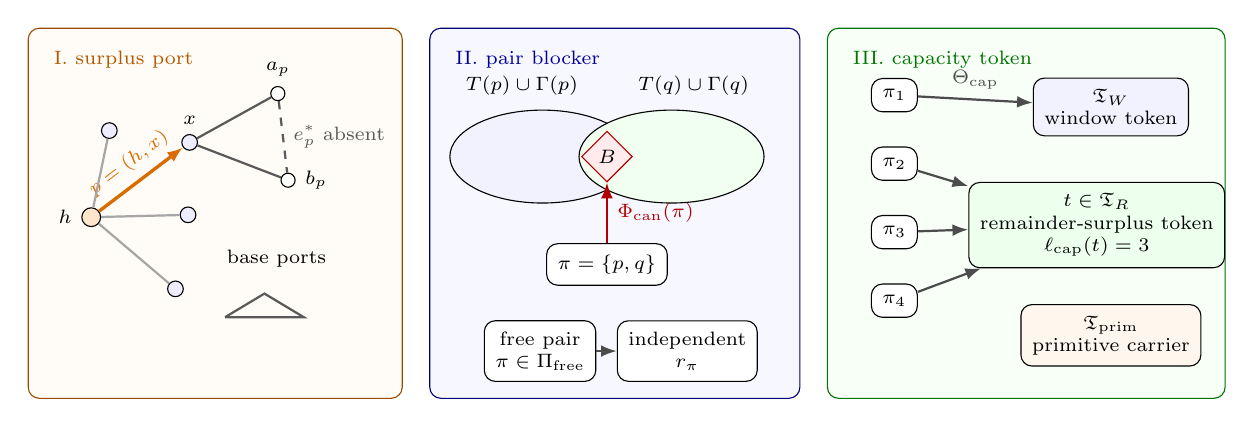
\begin{tikzpicture}[
vtx/.style={circle,draw,fill=white,inner sep=1.8pt},
high/.style={circle,draw=black,fill=orange!20,inner sep=2.4pt},
cubic/.style={circle,draw=black,fill=blue!7,inner sep=2.0pt},
support/.style={ellipse,draw,fill=blue!5,minimum width=2.35cm,minimum height=1.18cm,align=center},
supportq/.style={ellipse,draw,fill=green!6,minimum width=2.35cm,minimum height=1.18cm,align=center},
blocker/.style={diamond,draw=red!70!black,fill=red!8,inner sep=1.8pt,align=center},
token/.style={rectangle,rounded corners,draw,align=center,inner sep=4pt,fill=black!2},
edge/.style={thick,black!65},
port/.style={-{Latex[length=2mm]},very thick,orange!85!black},
arr/.style={-{Latex[length=2mm]},thick,black!70},
bad/.style={-{Latex[length=2mm]},thick,red!70!black},
box/.style={rectangle,rounded corners,draw,align=left,inner sep=4pt,fill=black!2},
every node/.style={font=\scriptsize}
]
% Panel frames.
\draw[rounded corners,fill=orange!3,draw=orange!60!black] (-7.45,-2.15) rectangle (-2.70,2.55);
\draw[rounded corners,fill=blue!3,draw=blue!45!black] (-2.35,-2.15) rectangle (2.35,2.55);
\draw[rounded corners,fill=green!3,draw=green!45!black] (2.70,-2.15) rectangle (7.75,2.55);
\node[anchor=north west,orange!70!black] at (-7.25,2.38) {I. surplus port};
\node[anchor=north west,blue!60!black] at (-2.15,2.38) {II. pair blocker};
\node[anchor=north west,green!45!black] at (2.90,2.38) {III. capacity token};

% Panel I: high centre and selected port.
\node[high,label=left:$h$] (h) at (-6.65,0.15) {};
\node[cubic,label=above:$x$] (x) at (-5.40,1.10) {};
\node[vtx,label=above:$a_p$] (a) at (-4.28,1.72) {};
\node[vtx,label=right:$b_p$] (b) at (-4.15,0.62) {};
\draw[port] (h)--node[above,sloped] {$p=(h,x)$} (x);
\draw[edge] (x)--(a);
\draw[edge] (x)--(b);
\draw[edge,dashed] (a)--node[right] {$e_p^*$ absent} (b);
\node[cubic] (u1) at (-5.42,0.18) {};
\node[cubic] (u2) at (-5.58,-0.76) {};
\node[cubic] (u3) at (-6.42,1.25) {};
\draw[edge,black!35] (h)--(u1);
\draw[edge,black!35] (h)--(u2);
\draw[edge,black!35] (h)--(u3);
\node[anchor=west] at (-5.05,-0.38) {base ports};
\draw[edge] (-4.95,-1.12)--(-4.45,-0.82)--(-3.95,-1.12)--(-4.95,-1.12);

% Panel II: blocker/free split.
\node[support] (sp) at (-0.92,0.92) {};
\node[anchor=south] at (-1.18,1.57) {\(T(p)\cup\Gamma(p)\)};
\node[supportq] (sq) at (0.72,0.92) {};
\node[anchor=south] at (1.00,1.57) {\(T(q)\cup\Gamma(q)\)};
\node[blocker] (B) at (-0.10,0.92) {\(B\)};
\node[token,fill=white] (pi) at (-0.10,-0.45) {\(\pi=\{p,q\}\)};
\draw[bad] (pi)--node[right] {\(\Phi_{\rm can}(\pi)\)} (B);
\node[token,fill=white] (free) at (-0.95,-1.55) {free pair\\ \(\pi\in\Pi_{\rm free}\)};
\node[token,fill=white] (resp) at (0.92,-1.55) {independent\\ \(r_\pi\)};
\draw[arr] (free)--(resp);

% Panel III: token assignment and load.
\node[token,fill=white] (pi1) at (3.55,1.70) {\(\pi_1\)};
\node[token,fill=white] (pi2) at (3.55,0.83) {\(\pi_2\)};
\node[token,fill=white] (pi3) at (3.55,-0.04) {\(\pi_3\)};
\node[token,fill=white] (pi4) at (3.55,-0.91) {\(\pi_4\)};
\node[token,fill=blue!5] (tw) at (6.30,1.55) {\(\mathfrak T_W\)\\ window token};
\node[token,fill=green!7,minimum width=3.20cm] (tr) at (6.12,0.05) {\(t\in\mathfrak T_R\)\\ remainder-surplus token\\ \(\ell_{\rm cap}(t)=3\)};
\node[token,fill=orange!7] (tp) at (6.30,-1.35) {\(\mathfrak T_{\rm prim}\)\\ primitive carrier};
\draw[arr] (pi1)--node[above] {\(\Theta_{\rm cap}\)} (tw);
\draw[arr] (pi2)--(tr);
\draw[arr] (pi3)--(tr);
\draw[arr] (pi4)--(tr);
\end{tikzpicture}%
}
\caption[Visual definition of the sparse surplus token ledger]{Visual definition of the sparse surplus port, blocker, and capacity-token ledger.  Panel I shows a high center \(h\), a selected surplus port \(p=(h,x)\), and the cubic endpoint \(x\) with its two shoulder vertices \(a_p,b_p\).  The dashed shoulder chord \(e_p^*=a_pb_p\) illustrates an open port; the small triangle below illustrates the triangular case \(e_p^*\in E(G)\).  The selected ports in \(\mathcal P_{\rm exc}(h)\) are the \(d_G(h)-3\) surplus units at \(h\), while the unselected incidences are base ports.  Panel II shows two active demands \(p,q\), their declared supports \(T(p)\cup\Gamma(p)\) and \(T(q)\cup\Gamma(q)\), and a blocker \(B\) for the pair \(\pi=\{p,q\}\).  A blocked pair is assigned its canonical blocker \(\Phi_{\rm can}(\pi)\); a free pair lies in \(\Pi_{\rm free}\) and contributes an independent pair-response coordinate \(r_\pi\).  Panel III shows the capacity-token map \(\Theta_{\rm cap}\).  Each blocked pair is assigned exactly one token in the disjoint union \(\mathfrak T_{\rm cap}=\mathfrak T_W\sqcup\mathfrak T_R\sqcup\mathfrak T_{\rm prim}\), where \(\mathfrak T_W\) records window incidences, \(\mathfrak T_R\) records surplus units in the remainder, and \(\mathfrak T_{\rm prim}\) records primitive carriers.  Multiple blocked pairs may land on the same token \(t\); their number is the token load \(\ell_{\rm cap}(t)=|\Theta_{\rm cap}^{-1}(t)|\).}
\label{fig:sparse-surplus-token-gadget}
\end{figure}

\begin{lemma}[Capacity-token supply]\label[lemma]{lem:capacity-token-supply}
The capacity-token universe satisfies
\[
|\mathfrak T_{\rm cap}|
\le
8n+\sigma(G).
\]
More precisely,
\[
|\mathfrak T_{\rm cap}|
=
|\mathfrak U_{\rm sp}(G)|+\sigma_R+e(R,W)+2e_\times(W)
=
|\mathfrak U_{\rm sp}(G)|+15p_{13}+\sigma(G).
\]
\end{lemma}

\begin{proof}
By construction,
\[
|\mathfrak T_{\rm cap}|
=
|\mathfrak T_{\rm prim}|+|\mathfrak T_R|+|\mathfrak T_W|
=
|\mathfrak U_{\rm sp}(G)|+\sigma_R+e(R,W)+2e_\times(W).
\]
The exact window-join identity \cref{lem:exact-window-join-identity} gives
\[
e(R,W)+2e_\times(W)=15p_{13}+\sigma_W.
\]
Since \(\sigma(G)=\sigma_R+\sigma_W\),
\[
|\mathfrak T_{\rm cap}|
=|\mathfrak U_{\rm sp}(G)|+15p_{13}+\sigma(G).
\]
By \cref{lem:primitive-carrier-supply}, \(|\mathfrak U_{\rm sp}(G)|\le6n\).
Also \(13p_{13}\le n\), because the packed \(P_{13}\) windows are
vertex-disjoint.  Hence \(15p_{13}\le(15/13)n<2n\), and therefore
\[
|\mathfrak T_{\rm cap}|\le8n+\sigma(G).
\]
\end{proof}

\begin{lemma}[Token ledger has no overcounting]\label[lemma]{lem:token-ledger-no-overcount}
For every finite family \(\mathcal A_0\) of active surplus demands,
\[
|\Pi_{\rm blk}|
=
\sum_{t\in\mathfrak T_{\rm cap}}\ell_{\rm cap}(t).
\]
Consequently, if \(\ell_{\rm cap}(t)\le M_0\) for every
\(t\in\mathfrak T_{\rm cap}\), then
\[
|\Pi_{\rm blk}|
\le
M_0(8n+\sigma(G)).
\]
\end{lemma}

\begin{proof}
The map \(\Theta_{\rm cap}:\Pi_{\rm blk}\to\mathfrak T_{\rm cap}\) assigns
exactly one token to each blocked pair.  The fibres
\(\Theta_{\rm cap}^{-1}(t)\), \(t\in\mathfrak T_{\rm cap}\), form a disjoint
partition of \(\Pi_{\rm blk}\).  Therefore
\[
|\Pi_{\rm blk}|
=
\sum_{t\in\mathfrak T_{\rm cap}}|\Theta_{\rm cap}^{-1}(t)|
=
\sum_{t\in\mathfrak T_{\rm cap}}\ell_{\rm cap}(t).
\]
If every token load is at most \(M_0\), then
\[
|\Pi_{\rm blk}|
\le
M_0|\mathfrak T_{\rm cap}|
\le
M_0(8n+\sigma(G))
\]
by \cref{lem:capacity-token-supply}.
\end{proof}

\begin{definition}[Token-fibre graphs and same-token patterns]\label[definition]{def:same-token-patterns}
For \(t\in\mathfrak T_{\rm cap}\), the \emph{token-fibre graph} \(H_t\) is
the simple graph with vertex set \(\mathcal A_0\) and edge set
\[
E(H_t)=\Pi_t=\Theta_{\rm cap}^{-1}(t).
\]
Thus
\[
e(H_t)=\ell_{\rm cap}(t).
\]
A \emph{same-token \(K\)-matching} at \(t\) is a matching of size \(K\) in
\(H_t\).  A \emph{same-token \(K\)-star} at \(t\) is a set of \(K\) edges of
\(H_t\) incident with one common active demand.  The token class of the pattern
is the token class containing \(t\): window-incidence, remainder-surplus, or
primitive-carrier.
\end{definition}

\begin{definition}[Same-token blocker roles]\label[definition]{def:same-token-blocker-roles}
Let \(t\in\mathfrak T_{\rm cap}\), and let
\(\pi\in\Theta_{\rm cap}^{-1}(t)\).  Put \(B_\pi=\Phi_{\rm can}(\pi)\).
The \emph{same-token role} of \(\pi\) at \(t\) is the following finite label:
\[
\rho_t(\pi)=
\bigl(\operatorname{type}(B_\pi),\operatorname{class}(t),
\operatorname{sub}(t)\bigr).
\]
Here \(\operatorname{type}(B_\pi)\in\{a,b,c,d,e,f\}\) is the blocker type in
\cref{def:surplus-blockers}.  The token class
\(\operatorname{class}(t)\) is one of \(W,R,P\), according as
\[
t\in\mathfrak T_W,\qquad t\in\mathfrak T_R,\qquad
t\in\mathfrak T_{\rm prim}.
\]
The subtype is defined by
\[
\operatorname{sub}(t)=
\begin{cases}
RW, & t=(e,RW)\in\mathfrak T_W,\\
WW, & t=(e,a)\in\mathfrak T_W\text{ is a cross-window endpoint token},\\
R, & t\in\mathfrak T_R,\\
V, & t\in V(G)\subseteq\mathfrak T_{\rm prim},\\
I, & t\in I_E(G)\subseteq\mathfrak T_{\rm prim},\\
P, & t\in\mathcal P_{\rm exc}\subseteq\mathfrak T_{\rm prim}.
\end{cases}
\]
Let \(\mathfrak R_{\rm st}\) be the set of all such labels.  Then
\[
|\mathfrak R_{\rm st}|\le 6(2+1+3)=36.
\]
We write \(Q_{\rm st}:=36\) for this uniform role bound.
For \(r\in\mathfrak R_{\rm st}\), define the \emph{role fibre} at \(t\) by
\[
\Pi_{t,r}:=\{\pi\in\Theta_{\rm cap}^{-1}(t):\rho_t(\pi)=r\},
\qquad
\ell(t,r):=|\Pi_{t,r}|.
\]
The role-fibre graph \(H_{t,r}\) is the spanning subgraph of \(H_t\) with edge
set \(\Pi_{t,r}\).  The sets \(\Pi_{t,r}\), \(r\in\mathfrak R_{\rm st}\),
partition \(\Theta_{\rm cap}^{-1}(t)\), and therefore
\[
\ell_{\rm cap}(t)=\sum_{r\in\mathfrak R_{\rm st}}\ell(t,r).
\]
A same-token matching or same-token star is \emph{role-homogeneous} if all of
its edges \(\pi\) have the same label \(\rho_t(\pi)\).
\end{definition}

\begin{definition}[Token-load threshold and homogeneous cap charge]\label[definition]{def:homogeneous-token-charge}
For \(x\ge0\), define
\[
\psi(x):=
\begin{cases}
0, & x=0,\\[2mm]
\left\lceil\dfrac{1+\sqrt{1+8x}}4\right\rceil, & x>0.
\end{cases}
\]
Equivalently, \(\psi(x)\) is the least integer \(k\ge0\) such that
\[
x\le k(2k-1).
\]
For an integer \(L\ge1\), define the \emph{role-homogeneous token cap charge}
\[
\operatorname{Cap}_{\rm hom}(L):=
Q_{\rm st}(L-1)(2L-3).
\]
Thus \(\operatorname{Cap}_{\rm hom}(L)\) is the uniform token load allowed by
charging each of the at most \(Q_{\rm st}\) role fibres separately when no
role-homogeneous same-token \(L\)-matching or \(L\)-star occurs at that token.
\end{definition}

\begin{lemma}[Homogeneous extraction from a same-token overload]\label[lemma]{lem:same-token-homogeneous-extraction}
If a token \(t\in\mathfrak T_{\rm cap}\) supports a same-token \(K\)-matching,
then \(t\) supports a role-homogeneous same-token matching of size at least
\(\lceil K/Q_{\rm st}\rceil\).  If \(t\) supports a same-token \(K\)-star, then
\(t\) supports a role-homogeneous same-token star of size at least
\(\lceil K/Q_{\rm st}\rceil\).
\end{lemma}

\begin{proof}
The edges of \(H_t\) are coloured by the role map
\(\rho_t:E(H_t)\to\mathfrak R_{\rm st}\).  By
\cref{def:same-token-blocker-roles}, at most \(Q_{\rm st}=36\) colours occur.
If \(M\) is a same-token \(K\)-matching, then the sets
\[
M_r:=\{\pi\in M:\rho_t(\pi)=r\},
\qquad r\in\mathfrak R_{\rm st},
\]
partition \(M\).  Hence one colour class has cardinality at least
\(\lceil K/Q_{\rm st}\rceil\).  That colour class is still a matching, because
it is a subset of \(M\), and it is role-homogeneous by construction.

The star case is identical.  If \(S\) is a same-token \(K\)-star with centre
\(p\), then each colour class \(S_r\subseteq S\) is still a star with the same
centre \(p\).  One colour class has size at least
\(\lceil K/Q_{\rm st}\rceil\).
\end{proof}

\begin{corollary}[Homogeneous same-token caps close the surplus branch]\label[corollary]{cor:homogeneous-same-token-caps-close}
Assume \(G\) survives the sparse surplus exits, admits a baseline spine demand
with \(E_{\rm spine}(n)\le C_E n\), and has full active family
\(\mathcal A_0=\mathcal P_{\rm exc}\).  Suppose there are fixed integers
\(L_W,L_R,L_P\) such that:
\begin{enumerate}[label=(\alph*), leftmargin=2.2em]
\item no token in \(\mathfrak T_W\) supports a role-homogeneous same-token
\(L_W\)-matching or role-homogeneous same-token \(L_W\)-star;
\item no token in \(\mathfrak T_R\) supports a role-homogeneous same-token
\(L_R\)-matching or role-homogeneous same-token \(L_R\)-star;
\item no token in \(\mathfrak T_{\rm prim}\) supports a role-homogeneous
same-token \(L_P\)-matching or role-homogeneous same-token \(L_P\)-star.
\end{enumerate}
Then
\[
\sigma(G)=O(\sqrt n),
\]
where the implicit constant depends only on \(C_E,L_W,L_R,L_P\).
\end{corollary}

\begin{proof}
Let
\[
M_0:=\max\{
\operatorname{Cap}_{\rm hom}(L_W),\
\operatorname{Cap}_{\rm hom}(L_R),\
\operatorname{Cap}_{\rm hom}(L_P)\}.
\]
We show that every token has load at most \(M_0\).  Fix
\(t\in\mathfrak T_W\).  For each role \(r\), the graph \(H_{t,r}\) has no
\(L_W\)-matching and no \(L_W\)-star; otherwise that matching or star would be
a role-homogeneous same-token \(L_W\)-pattern at \(t\), contrary to (a).  By
\cref{lem:same-token-matching-star},
\[
\ell(t,r)\le (L_W-1)(2L_W-3)
\]
for every \(r\).  Summing the role-fibre partition of
\cref{def:same-token-blocker-roles} gives
\[
\ell_{\rm cap}(t)
=\sum_{r\in\mathfrak R_{\rm st}}\ell(t,r)
\le Q_{\rm st}(L_W-1)(2L_W-3)
=\operatorname{Cap}_{\rm hom}(L_W)
\le M_0 .
\]
The argument for a token in \(\mathfrak T_W\) used only the role-fibre
partition and the corresponding homogeneous cap.  Replacing \(L_W\) by \(L_R\)
or \(L_P\) gives the same bound for tokens in
\(\mathfrak T_R\) and \(\mathfrak T_{\rm prim}\).  The hypotheses of
\cref{thm:tokenized-surplus-accounting-closure} now hold with \(c_1=1\),
because \(|\mathcal A_0|=\sigma(G)\) by
\cref{lem:surviving-active-family}.  That theorem gives
\(\sigma(G)=O(\sqrt n)\).
\end{proof}

\begin{corollary}[Forced homogeneous same-token scale]\label[corollary]{cor:forced-homogeneous-same-token-scale}
Assume \(G\) survives the sparse surplus exits, admits a baseline spine demand
with deficit \(E_{\rm spine}(n)\), and has full active family
\(\mathcal A_0=\mathcal P_{\rm exc}\).  Let \(\Lambda(G)\) be the quantity in
\cref{cor:forced-same-token-scale}.  Then some capacity token supports a
role-homogeneous same-token matching or role-homogeneous same-token star of
size at least
\[
\psi\!\left(\frac{\Lambda(G)}{Q_{\rm st}}\right).
\]
In particular, if \(E_{\rm spine}(n)=O(n)\) and
\(\sigma(G)/\sqrt n\to\infty\), then the forced role-homogeneous same-token
matching-or-star size tends to infinity.
\end{corollary}

\begin{proof}
\Cref{lem:capacity-token-high-load} gives a token \(t\) with
\[
\ell_{\rm cap}(t)\ge\Lambda(G).
\]
The role fibres at \(t\) partition \(\Theta_{\rm cap}^{-1}(t)\), so
\[
\sum_{r\in\mathfrak R_{\rm st}}\ell(t,r)=\ell_{\rm cap}(t).
\]
Since at most \(Q_{\rm st}\) roles occur, some role \(r\) satisfies
\[
\ell(t,r)\ge\frac{\Lambda(G)}{Q_{\rm st}}.
\]
Apply \cref{lem:same-token-matching-star} to the role-fibre graph \(H_{t,r}\).
If \(s=\max\{\nu(H_{t,r}),\Delta(H_{t,r})\}\), then
\[
\ell(t,r)=e(H_{t,r})\le s(2s-1).
\]
By the definition of \(\psi\),
\[
s\ge\psi\!\left(\frac{\Lambda(G)}{Q_{\rm st}}\right).
\]
Thus \(H_{t,r}\) contains a matching or star of that size.  Because all edges
of \(H_{t,r}\) have the same role \(r\), this is a role-homogeneous same-token
matching or star.  The final assertion follows because \(Q_{\rm st}\) is
fixed.
\end{proof}

\begin{corollary}[Quantitative homogeneous overload lower bound]\label[corollary]{cor:quantitative-homogeneous-overload}
Assume \(G\) survives the sparse surplus exits, has full active family
\(\mathcal A_0=\mathcal P_{\rm exc}\), and admits a baseline spine demand with
deficit \(E_{\rm spine}(n)\le C_E n\).  Let \(K_{\rm hom}(G)\) be the largest
integer \(K\) for which some capacity token supports a role-homogeneous
same-token \(K\)-matching or a role-homogeneous same-token \(K\)-star.  Then
\[
K_{\rm hom}(G)\ge
\psi\!\left(
\frac{
\max\left\{0,\,
\binom{\sigma(G)}2
-C_E n
-\left(\frac12\sigma(G)+1\right)\log_2 n
\right\}}
{Q_{\rm st}(8n+\sigma(G))}
\right).
\]
Consequently:
\begin{enumerate}[label=(\alph*), leftmargin=2.2em]
\item If \(\sigma(G)\ge A\sqrt n\), \(A^2\ge6(C_E+1)\), and \(n\) is
sufficiently large in terms of \(A\) and \(C_E\), then
\[
K_{\rm hom}(G)\ge
\left\lceil\frac{A}{12\sqrt{Q_{\rm st}}}\right\rceil .
\]
\item If \(\sigma(G)\ge\alpha n\) for some fixed \(\alpha>0\), and \(n\) is
sufficiently large in terms of \(\alpha\) and \(C_E\), then
\[
K_{\rm hom}(G)\ge
\left\lceil\frac{\alpha}{12\sqrt{Q_{\rm st}}}\sqrt n\right\rceil .
\]
\end{enumerate}
\end{corollary}

\begin{proof}
The displayed bound is \cref{cor:forced-homogeneous-same-token-scale} with
\(E_{\rm spine}(n)\le C_E n\) substituted into \(\Lambda(G)\).

For (a), assume \(\sigma(G)\ge A\sqrt n\).  Since
\(\sigma(G)\le n\) by \cref{lem:sparse-upper-envelope}, the denominator
\(8n+\sigma(G)\) is at most \(9n\).  For fixed \(A\), the term
\((\sigma(G)/2+1)\log_2 n\) is \(o(n)\).  For all sufficiently large \(n\),
\[
\binom{\sigma(G)}2
-C_E n
-\left(\frac12\sigma(G)+1\right)\log_2 n
\ge
\left(\frac{A^2}{3}-C_E-1\right)n
\ge
\frac{A^2}{6}n ,
\]
where the last inequality uses \(A^2\ge6(C_E+1)\).  Hence
\[
\frac{
\binom{\sigma(G)}2
-C_E n
-\left(\frac12\sigma(G)+1\right)\log_2 n}
{Q_{\rm st}(8n+\sigma(G))}
\ge
\frac{A^2}{54Q_{\rm st}}.
\]
If \(k<A/(12\sqrt{Q_{\rm st}})\), then
\[
k(2k-1)<2k^2<\frac{A^2}{72Q_{\rm st}}
<\frac{A^2}{54Q_{\rm st}}.
\]
By the defining minimality of \(\psi\), this gives (a).

For (b), assume \(\sigma(G)\ge\alpha n\).  For all sufficiently large \(n\),
\[
\binom{\sigma(G)}2
-C_E n
-\left(\frac12\sigma(G)+1\right)\log_2 n
\ge \frac{\alpha^2}{3}n^2 .
\]
Again \(8n+\sigma(G)\le9n\).  Therefore
\[
\frac{
\binom{\sigma(G)}2
-C_E n
-\left(\frac12\sigma(G)+1\right)\log_2 n}
{Q_{\rm st}(8n+\sigma(G))}
\ge
\frac{\alpha^2}{27Q_{\rm st}}n .
\]
If \(k<\alpha\sqrt n/(12\sqrt{Q_{\rm st}})\), then
\[
k(2k-1)<2k^2
<\frac{\alpha^2}{72Q_{\rm st}}n
<\frac{\alpha^2}{27Q_{\rm st}}n.
\]
The defining minimality of \(\psi\) gives (b).
\end{proof}

\begin{lemma}[Matching--star accounting]\label[lemma]{lem:same-token-matching-star}
Let \(H\) be a finite simple graph with \(e(H)\) edges, matching number
\(\nu(H)\), and maximum degree \(\Delta(H)\).  Then
\[
e(H)\le \nu(H)\bigl(2\Delta(H)-1\bigr).
\]
Consequently, if \(K\ge1\) and \(H\) contains neither a matching of size \(K\)
nor a star of size \(K\), then
\[
e(H)\le (K-1)(2K-3).
\]
Equivalently, if \(e(H)>(K-1)(2K-3)\), then \(H\) contains a matching of size
\(K\) or a star of size \(K\).
\end{lemma}

\begin{proof}
Choose a maximum matching \(M\) in \(H\).  Since \(M\) is maximal, every edge
of \(H\) has at least one endpoint in the set \(U\) of vertices covered by
\(M\).  Thus \(U\) is a vertex cover of \(H\), and \(|U|=2\nu(H)\).  Each
vertex of \(U\) is incident with at most \(\Delta(H)\) edges of \(H\).  Hence
\[
\sum_{u\in U}d_H(u)\le2\nu(H)\Delta(H).
\]
The \(\nu(H)\) matching edges of \(M\) have both endpoints in \(U\), and are
therefore counted twice in the degree sum.  Every other edge is counted at
least once, because \(U\) is a vertex cover.  Hence
\[
e(H)
\le
\sum_{u\in U}d_H(u)-\nu(H)
\le
\nu(H)\bigl(2\Delta(H)-1\bigr).
\]
If \(H\) contains no matching of size \(K\), then \(\nu(H)\le K-1\).  If it
contains no star of size \(K\), then \(\Delta(H)\le K-1\).  Substituting these
two bounds gives \(e(H)\le(K-1)(2K-3)\).  The final statement is the
contrapositive.
\end{proof}

\begin{corollary}[Same-token pattern caps close the surplus branch]\label[corollary]{cor:same-token-pattern-caps-close}
Assume \(G\) survives the sparse surplus exits, admits a baseline spine demand
with \(E_{\rm spine}(n)\le C_E n\), and has full active family
\(\mathcal A_0=\mathcal P_{\rm exc}\).  Suppose there are fixed integers
\(K_W,K_R,K_P\) such that:
\begin{enumerate}[label=(\alph*), leftmargin=2.2em]
\item no token in \(\mathfrak T_W\) supports a same-token \(K_W\)-matching or
a same-token \(K_W\)-star;
\item no token in \(\mathfrak T_R\) supports a same-token \(K_R\)-matching or
a same-token \(K_R\)-star;
\item no token in \(\mathfrak T_{\rm prim}\) supports a same-token
\(K_P\)-matching or a same-token \(K_P\)-star.
\end{enumerate}
Then
\[
\sigma(G)=O(\sqrt n),
\]
where the implicit constant depends only on \(C_E,K_W,K_R,K_P\).
\end{corollary}

\begin{proof}
Put
\[
M_0:=\max\bigl\{
(K_W-1)(2K_W-3),\,
(K_R-1)(2K_R-3),\,
(K_P-1)(2K_P-3)
\bigr\}.
\]
By \cref{lem:same-token-matching-star}, every token load satisfies
\[
\ell_{\rm cap}(t)\le M_0 .
\]
The hypotheses of \cref{thm:tokenized-surplus-accounting-closure} now hold
with \(c_1=1\), because
\(|\mathcal A_0|=\sigma(G)\) by \cref{lem:surviving-active-family}.  That
theorem gives \(\sigma(G)=O(\sqrt n)\).
\end{proof}

\begin{corollary}[Forced same-token overload scale]\label[corollary]{cor:forced-same-token-scale}
Assume \(G\) survives the sparse surplus exits, admits a baseline spine demand
with deficit \(E_{\rm spine}(n)\), and has full active family
\(\mathcal A_0=\mathcal P_{\rm exc}\).  Put
\[
\Lambda(G):=
\frac{
\max\left\{0,\,
\binom{\sigma(G)}2
-E_{\rm spine}(n)
-\left(\frac12\sigma(G)+1\right)\log_2 n
\right\}}
{8n+\sigma(G)} .
\]
Then some capacity token supports a same-token matching or a same-token star of
size at least
\[
\psi(\Lambda(G)).
\]
In particular, if \(E_{\rm spine}(n)=O(n)\) and
\(\sigma(G)/\sqrt n\to\infty\), then the forced same-token matching-or-star
size tends to infinity.
\end{corollary}

\begin{proof}
\Cref{lem:capacity-token-high-load} gives a token \(t\) with
\[
\ell_{\rm cap}(t)\ge \Lambda(G).
\]
Let \(r=\max\{\nu(H_t),\Delta(H_t)\}\).  By
\cref{lem:same-token-matching-star},
\[
\ell_{\rm cap}(t)=e(H_t)\le r(2r-1).
\]
Since \(\ell_{\rm cap}(t)\ge\Lambda(G)\), the definition of \(\psi\) gives
\[
r\ge\psi(\Lambda(G)).
\]
Thus \(H_t\) contains either a matching or a star of size
\(\psi(\Lambda(G))\), which is precisely a same-token matching or same-token
star at \(t\).  If
\(E_{\rm spine}(n)=O(n)\) and \(\sigma(G)/\sqrt n\to\infty\), then the
numerator in \(\Lambda(G)\) is \(\frac12\sigma(G)^2-o(\sigma(G)^2)\), while
\(8n+\sigma(G)\le9n\) by \(\sigma(G)\le n\), which follows from
\cref{lem:sparse-upper-envelope}.  Hence
\(\Lambda(G)\to\infty\), and so the displayed same-token pattern size tends to
infinity.
\end{proof}

\begin{lemma}[Exact surplus-pair charge partition]\label[lemma]{lem:exact-surplus-pair-charge-partition}
Let \(\mathcal A_0\) be a finite family of active surplus demands.  For
\(C\in\{W,R,P\}\), use the token classes
\[
\mathfrak T_W,\qquad \mathfrak T_R,\qquad
\mathfrak T_P:=\mathfrak T_{\rm prim}.
\]
Then the following disjoint union is exact:
\[
\binom{\mathcal A_0}{2}
=
\Pi_{\rm free}
\sqcup
\bigsqcup_{C\in\{W,R,P\}}
\bigsqcup_{t\in\mathfrak T_C}
\bigsqcup_{r\in\mathfrak R_{\rm st}}
\Pi_{t,r}.
\]
Consequently,
\[
\binom{|\mathcal A_0|}{2}
=
|\Pi_{\rm free}|
+
\sum_{C\in\{W,R,P\}}
\sum_{t\in\mathfrak T_C}
\sum_{r\in\mathfrak R_{\rm st}}
\ell(t,r).
\]
Every unordered pair of active demands appears in exactly one summand on the
right-hand side.
\end{lemma}

\begin{proof}
By \cref{def:canonical-blocker-ledger}, the pair set
\(\binom{\mathcal A_0}{2}\) is the disjoint union
\[
\Pi_{\rm free}\sqcup\Pi_{\rm blk}.
\]
If \(\pi\in\Pi_{\rm blk}\), then \(\Theta_{\rm cap}(\pi)\) is defined and is a
single element of the disjoint token universe
\[
\mathfrak T_{\rm cap}
=\mathfrak T_W\sqcup\mathfrak T_R\sqcup\mathfrak T_{\rm prim}.
\]
Thus \(\pi\) lies in exactly one token class \(C\) and exactly one token
\(t\in\mathfrak T_C\).  For that fixed \(t\), the role map
\(\rho_t\) assigns exactly one role \(r\in\mathfrak R_{\rm st}\), so
\(\pi\in\Pi_{t,r}\).  This proves that every blocked pair appears in at least
one displayed role-fibre summand.

The appearance is unique.  The token classes are disjoint, \(\Theta_{\rm cap}\)
is a function, and \(\rho_t\) is a function once \(t\) is fixed.  Hence a
blocked pair cannot belong to two distinct triples \((C,t,r)\).  Conversely,
every \(\Pi_{t,r}\) is a subset of \(\Theta_{\rm cap}^{-1}(t)\subseteq
\Pi_{\rm blk}\), so no free pair appears in any role-fibre summand.  Therefore
the displayed union is disjoint and exhaustive.  Taking cardinalities gives the
second formula.
\end{proof}

\begin{theorem}[Sharp classwise homogeneous token budget]\label[theorem]{thm:sharp-classwise-homogeneous-token-budget}
Assume \(G\) survives the sparse surplus exits, admits a baseline spine demand
with deficit \(E_{\rm spine}(n)\), and has full active family
\(\mathcal A_0=\mathcal P_{\rm exc}\).  Put
\[
N_*(G):=
\max\left\{0,\,
\binom{\sigma(G)}2
-E_{\rm spine}(n)
-\left(\frac12\sigma(G)+1\right)\log_2 n
\right\}.
\]
For \(C\in\{W,R,P\}\), set
\[
\mathfrak T_C=
\begin{cases}
\mathfrak T_W,&C=W,\\
\mathfrak T_R,&C=R,\\
\mathfrak T_{\rm prim},&C=P,
\end{cases}
\qquad
\Pi_C:=\{\pi\in\Pi_{\rm blk}:\Theta_{\rm cap}(\pi)\in\mathfrak T_C\},
\]
and write \(B_C:=|\Pi_C|\), \(S_C:=|\mathfrak T_C|\).  Then:
\begin{enumerate}[label=(\alph*), leftmargin=2.2em]
\item The blocked-pair demand satisfies the exact class split
\[
B_W+B_R+B_P=|\Pi_{\rm blk}|\ge N_*(G).
\]
\item The class supplies are
\[
S_W=15p_{13}+\sigma_W,\qquad
S_R=\sigma_R,\qquad
S_P=|\mathfrak U_{\rm sp}(G)|\le6n,
\]
and hence
\[
S_W+S_R+S_P\le8n+\sigma(G).
\]
\item If no token in \(\mathfrak T_C\) supports a role-homogeneous same-token
\(L_C\)-matching or role-homogeneous same-token \(L_C\)-star, then
\[
B_C\le \operatorname{Cap}_{\rm hom}(L_C)S_C
=Q_{\rm st}(L_C-1)(2L_C-3)S_C .
\]
\item If the three homogeneous caps \(L_W,L_R,L_P\) hold in the three token
classes, then the necessary classwise budget inequality is
\[
N_*(G)
\le
\operatorname{Cap}_{\rm hom}(L_W)(15p_{13}+\sigma_W)
+\operatorname{Cap}_{\rm hom}(L_R)\sigma_R
+\operatorname{Cap}_{\rm hom}(L_P)|\mathfrak U_{\rm sp}(G)|.
\]
In particular,
\[
N_*(G)
\le
\operatorname{Cap}_{\rm hom}(L_W)(15p_{13}+\sigma_W)
+\operatorname{Cap}_{\rm hom}(L_R)\sigma_R
+6\operatorname{Cap}_{\rm hom}(L_P)n .
\]
\item If \(N_*(G)>0\), then for some nonempty token class \(C\) there is a
token \(t\in\mathfrak T_C\) supporting a role-homogeneous same-token matching
or role-homogeneous same-token star of size at least
\[
\psi\!\left(\frac{B_C}{Q_{\rm st}S_C}\right),
\]
and in particular at least
\[
\psi\!\left(\frac{N_*(G)}{Q_{\rm st}(8n+\sigma(G))}\right).
\]
\end{enumerate}
\end{theorem}

\begin{proof}
For (a), the free-pair entropy sandwich with blockers gives
\[
|\Pi_{\rm free}|
\le
E_{\rm spine}(n)+\left(\frac12\sigma(G)+1\right)\log_2 n,
\]
because \(|\mathcal A_0|=\sigma(G)\).  Since
\[
|\Pi_{\rm free}|+|\Pi_{\rm blk}|=\binom{\sigma(G)}2,
\]
we obtain \(|\Pi_{\rm blk}|\ge N_*(G)\).  The three sets
\(\Pi_W,\Pi_R,\Pi_P\) partition \(\Pi_{\rm blk}\), because
\(\mathfrak T_{\rm cap}\) is the disjoint union
\(\mathfrak T_W\sqcup\mathfrak T_R\sqcup\mathfrak T_{\rm prim}\) and
\(\Theta_{\rm cap}\) assigns exactly one token to each blocked pair.  Hence
\[
B_W+B_R+B_P=|\Pi_{\rm blk}|\ge N_*(G).
\]

Part (b) is exactly \cref{lem:capacity-token-supply}, with
\(\mathfrak T_{\rm prim}=\mathfrak U_{\rm sp}(G)\) and
\cref{lem:primitive-carrier-supply} applied to \(S_P\).

For (c), fix a class \(C\) and a token \(t\in\mathfrak T_C\).  For every role
\(r\), the role-fibre graph \(H_{t,r}\) has no matching of size \(L_C\) and no
star of size \(L_C\); otherwise that matching or star would be a
role-homogeneous same-token \(L_C\)-pattern at \(t\).  By
\cref{lem:same-token-matching-star},
\[
\ell(t,r)=e(H_{t,r})\le (L_C-1)(2L_C-3).
\]
The role fibres partition the token fibre, so
\[
\ell_{\rm cap}(t)
=\sum_{r\in\mathfrak R_{\rm st}}\ell(t,r)
\le
Q_{\rm st}(L_C-1)(2L_C-3)
=\operatorname{Cap}_{\rm hom}(L_C).
\]
Summing the exact token fibres in class \(C\) gives
\[
B_C
=\sum_{t\in\mathfrak T_C}\ell_{\rm cap}(t)
\le
\operatorname{Cap}_{\rm hom}(L_C)S_C .
\]

Part (d) follows by summing the three estimates in (c) and using (a) and (b).

For (e), choose a class \(C\) for which \(B_C/S_C\) is maximal among nonempty
classes with \(S_C>0\).  Since the nonempty classes partition
\(\Pi_{\rm blk}\),
\[
\frac{B_C}{S_C}\ge
\frac{B_W+B_R+B_P}{S_W+S_R+S_P}
\ge
\frac{N_*(G)}{8n+\sigma(G)} .
\]
Some token \(t\in\mathfrak T_C\) then has load
\[
\ell_{\rm cap}(t)\ge B_C/S_C.
\]
The role fibres at \(t\) partition the token fibre, so some role \(r\) has
\[
\ell(t,r)\ge\frac{B_C}{Q_{\rm st}S_C}.
\]
Apply \cref{lem:same-token-matching-star} to \(H_{t,r}\).  If
\(s=\max\{\nu(H_{t,r}),\Delta(H_{t,r})\}\), then
\[
\ell(t,r)=e(H_{t,r})\le s(2s-1).
\]
Therefore
\[
s\ge\psi\!\left(\frac{B_C}{Q_{\rm st}S_C}\right).
\]
The graph \(H_{t,r}\) contains a matching or star of that size, and all its
edges have the same role \(r\).  This gives the first displayed homogeneous
lower bound.  The second follows from
\[
\frac{B_C}{S_C}\ge \frac{N_*(G)}{8n+\sigma(G)}
\]
and the monotonicity of \(\psi\).
\end{proof}

\begin{corollary}[Quantified homogeneous class overload]\label[corollary]{cor:quantified-homogeneous-class-overload}
Assume the hypotheses of
\cref{thm:sharp-classwise-homogeneous-token-budget}, and fix proposed
homogeneous caps \(L_W,L_R,L_P\).  Define the class capacities
\[
A_W:=\operatorname{Cap}_{\rm hom}(L_W)(15p_{13}+\sigma_W),\qquad
A_R:=\operatorname{Cap}_{\rm hom}(L_R)\sigma_R,\qquad
A_P:=\operatorname{Cap}_{\rm hom}(L_P)|\mathfrak U_{\rm sp}(G)|.
\]
Put
\[
D_{\rm exc}:=
\left(
N_*(G)-A_W-A_R-A_P
\right)_+,
\]
and, for \(C\in\{W,R,P\}\), put
\[
\Omega_C:=(B_C-A_C)_+ .
\]
Then:
\begin{enumerate}[label=(\alph*), leftmargin=2.2em]
\item The total class overload satisfies
\[
\Omega_W+\Omega_R+\Omega_P\ge D_{\rm exc}.
\]
\item Hence at least one class \(C\) satisfies
\[
\Omega_C\ge \frac13D_{\rm exc}.
\]
\item If \(\Omega_C>0\), then \(S_C>0\), and class \(C\) contains a
role-homogeneous same-token matching or role-homogeneous same-token star of
size at least
\[
\psi\!\left(
(L_C-1)(2L_C-3)+\frac{\Omega_C}{Q_{\rm st}S_C}
\right).
\]
\item If \(D_{\rm exc}>0\), and the two classes different from \(C\) do not
overload, i.e. \(B_{C'}\le A_{C'}\) for \(C'\ne C\), then class \(C\) overloads
by at least the whole deficit:
\[
\Omega_C\ge D_{\rm exc},
\]
and class \(C\) contains a role-homogeneous same-token matching or
role-homogeneous same-token star of size at least
\[
\psi\!\left(
(L_C-1)(2L_C-3)+\frac{D_{\rm exc}}{Q_{\rm st}S_C}
\right).
\]
\item The three pure-overload tests have the following sharp class-by-class
lower bounds.  Define
\[
F_W:=\bigl(N_*(G)-A_R-A_P\bigr)_+,\qquad
F_R:=\bigl(N_*(G)-A_W-A_P\bigr)_+,\qquad
F_P:=\bigl(N_*(G)-A_W-A_R\bigr)_+ .
\]
If \(B_R\le A_R\) and \(B_P\le A_P\), then
\[
B_W\ge F_W,\qquad
\Omega_W\ge(F_W-A_W)_+=D_{\rm exc}.
\]
If \(S_W>0\), the forced window-incidence homogeneous pattern has size at least
\[
\psi\!\left(\frac{F_W}{Q_{\rm st}S_W}\right).
\]
If \(B_W\le A_W\) and \(B_P\le A_P\), then
\[
B_R\ge F_R,\qquad
\Omega_R\ge(F_R-A_R)_+=D_{\rm exc}.
\]
If \(S_R>0\), the forced remainder-surplus homogeneous pattern has size at
least
\[
\psi\!\left(\frac{F_R}{Q_{\rm st}S_R}\right).
\]
If \(B_W\le A_W\) and \(B_R\le A_R\), then
\[
B_P\ge F_P,\qquad
\Omega_P\ge(F_P-A_P)_+=D_{\rm exc}.
\]
If \(S_P>0\), the forced primitive-carrier homogeneous pattern has size at
least
\[
\psi\!\left(\frac{F_P}{Q_{\rm st}S_P}\right).
\]
\end{enumerate}
The estimate is sharp for the scalar class-load ledger: the load vector
\[
B_C=A_C+D_{\rm exc},\qquad B_{C'}=A_{C'}\quad(C'\ne C)
\]
has total load \(A_W+A_R+A_P+D_{\rm exc}\) and overloads only class \(C\).
\end{corollary}

\begin{proof}
For (a), use the elementary inequality
\[
\sum_C (B_C-A_C)_+
\ge
\left(\sum_C B_C-\sum_C A_C\right)_+ .
\]
By \cref{thm:sharp-classwise-homogeneous-token-budget},
\[
\sum_C B_C=B_W+B_R+B_P\ge N_*(G),
\]
and therefore
\[
\Omega_W+\Omega_R+\Omega_P
\ge
\left(N_*(G)-A_W-A_R-A_P\right)_+
=D_{\rm exc}.
\]
Part (b) is the pigeonhole principle applied to the three nonnegative numbers
\(\Omega_W,\Omega_R,\Omega_P\).

For (c), if \(\Omega_C>0\), then \(B_C>A_C\), so \(B_C>0\), and hence
\(S_C>0\).  By
\cref{thm:sharp-classwise-homogeneous-token-budget}, class \(C\) contains a
role-homogeneous same-token matching or star of size at least
\[
\psi\!\left(\frac{B_C}{Q_{\rm st}S_C}\right).
\]
Since \(B_C=A_C+\Omega_C\) and
\[
A_C=\operatorname{Cap}_{\rm hom}(L_C)S_C
=Q_{\rm st}(L_C-1)(2L_C-3)S_C,
\]
we have
\[
\frac{B_C}{Q_{\rm st}S_C}
=(L_C-1)(2L_C-3)+\frac{\Omega_C}{Q_{\rm st}S_C}.
\]
This proves (c).

For (d), assume \(B_{C'}\le A_{C'}\) for the two classes \(C'\ne C\).  Then
\[
B_C
\ge
N_*(G)-\sum_{C'\ne C}B_{C'}
\ge
N_*(G)-\sum_{C'\ne C}A_{C'}
=
A_C+\left(N_*(G)-A_W-A_R-A_P\right).
\]
If \(D_{\rm exc}>0\), this gives \(B_C\ge A_C+D_{\rm exc}\), hence
\(\Omega_C\ge D_{\rm exc}\).  Substituting this bound into (c) gives the
displayed pattern-size lower bound.  The final sentence is a direct
substitution into the scalar identities defining the class-load ledger.

For (e), first assume \(B_R\le A_R\) and \(B_P\le A_P\).  Then
\[
B_W
\ge
N_*(G)-B_R-B_P
\ge
N_*(G)-A_R-A_P.
\]
Since \(B_W\ge0\), this gives \(B_W\ge F_W\).  Subtracting \(A_W\) and taking
positive parts gives
\[
\Omega_W\ge(F_W-A_W)_+
=\bigl(N_*(G)-A_W-A_R-A_P\bigr)_+
=D_{\rm exc}.
\]
If \(S_W>0\), then
\cref{thm:sharp-classwise-homogeneous-token-budget} gives a window-incidence
role-homogeneous same-token matching or star of size at least
\[
\psi\!\left(\frac{B_W}{Q_{\rm st}S_W}\right)
\ge
\psi\!\left(\frac{F_W}{Q_{\rm st}S_W}\right),
\]
using monotonicity of \(\psi\).  The \(R\)- and \(P\)-estimates are the same
argument with the class names permuted.
\end{proof}

\begin{corollary}[Coupled single-graph overload budget]\label[corollary]{cor:coupled-single-graph-overload-budget}
Assume the hypotheses of
\cref{thm:sharp-classwise-homogeneous-token-budget}, and fix proposed
homogeneous caps \(L_W,L_R,L_P\).  Put
\[
b_W:=(L_W-1)(2L_W-3),\qquad
b_R:=(L_R-1)(2L_R-3),\qquad
b_P:=(L_P-1)(2L_P-3).
\]
Since \(Q_{\rm st}=36\), the exact coupled capacity of the three classes in
the single graph \(G\) is
\[
A_{\rm all}
=
36\Bigl[
b_W(15p_{13}+\sigma_W)
+b_R\sigma_R
+b_P(4n+2\sigma(G))
\Bigr].
\]
Equivalently, using \(\sigma(G)=\sigma_W+\sigma_R\),
\[
A_{\rm all}
=
36\Bigl[
4b_Pn+15b_Wp_{13}
+(b_W+2b_P)\sigma_W
+(b_R+2b_P)\sigma_R
\Bigr].
\]
Define the coupled excess
\[
D_{\rm all}:=\bigl(N_*(G)-A_{\rm all}\bigr)_+ .
\]
Then:
\begin{enumerate}[label=(\alph*), leftmargin=2.2em]
\item The total role-fibre overload in the single graph is at least
\[
D_{\rm all}.
\]
\item The total number of role-fibre slots available to absorb this excess is
at most
\[
36\bigl(S_W+S_R+S_P\bigr)
=36\bigl(4n+15p_{13}+3\sigma(G)\bigr).
\]
\item If \(D_{\rm all}>0\), then for some class \(C\in\{W,R,P\}\) there is a
role fibre in that class whose load is at least
\[
b_C+
\frac{D_{\rm all}}
{36\bigl(4n+15p_{13}+3\sigma(G)\bigr)}.
\]
Consequently \(G\) contains a role-homogeneous same-token matching or
role-homogeneous same-token star of size at least
\[
\psi\!\left(
b_C+
\frac{D_{\rm all}}
{36\bigl(4n+15p_{13}+3\sigma(G)\bigr)}
\right)
\]
for that same class \(C\).
\end{enumerate}
\end{corollary}

\begin{proof}
The exact primitive-token supply is
\[
S_P=|\mathfrak U_{\rm sp}(G)|=n+2m+\sigma(G).
\]
Since \(\sigma(G)=2m-3n\), we have \(m=(3n+\sigma(G))/2\), and therefore
\[
S_P=n+2m+\sigma(G)=4n+2\sigma(G).
\]
Together with \(S_W=15p_{13}+\sigma_W\) and \(S_R=\sigma_R\), this gives the
displayed formula for \(A_{\rm all}\); the second displayed form is obtained by
substituting \(\sigma(G)=\sigma_W+\sigma_R\).

For each role fibre in class \(C\), the cap threshold before a homogeneous
\(L_C\)-matching or \(L_C\)-star is \(b_C\).  Thus the total role-fibre
capacity over all three classes is
\[
36b_WS_W+36b_RS_R+36b_PS_P=A_{\rm all}.
\]
Since the exact class theorem gives a blocked-pair demand at least \(N_*(G)\),
the excess above this coupled capacity is at least \(D_{\rm all}\).  This proves
(a).

The number of role-fibre slots is at most \(36(S_W+S_R+S_P)\).  Using the exact
supplies,
\[
S_W+S_R+S_P
=(15p_{13}+\sigma_W)+\sigma_R+(4n+2\sigma(G))
=4n+15p_{13}+3\sigma(G),
\]
which proves (b).

For a token \(t\in\mathfrak T_C\) and a role \(r\in\mathfrak R_{\rm st}\),
write
\[
E_{t,r}:=\bigl(\ell(t,r)-b_C\bigr)_+ .
\]
The elementary inequality \(\sum_i(x_i-y_i)_+\ge(\sum_i x_i-\sum_i y_i)_+\),
applied to all triples \((C,t,r)\), gives
\[
\sum_{C\in\{W,R,P\}}\sum_{t\in\mathfrak T_C}
\sum_{r\in\mathfrak R_{\rm st}}E_{t,r}
\ge
\left(
\sum_C B_C-A_{\rm all}
\right)_+
\ge D_{\rm all}.
\]
If \(D_{\rm all}>0\), distribute these explicitly defined role-fibre excesses
over the at most
\[
36\bigl(4n+15p_{13}+3\sigma(G)\bigr)
\]
role-fibre slots.  Some role fibre in some class \(C\) has excess at least the
average displayed in (c), so its load is at least
\[
b_C+
\frac{D_{\rm all}}
{36\bigl(4n+15p_{13}+3\sigma(G)\bigr)}.
\]
Applying the matching--star bound of \cref{lem:same-token-matching-star} to
that role-fibre graph gives the stated homogeneous matching-or-star lower
bound by the definition of \(\psi\).
\end{proof}

\begin{corollary}[Numerical normalized single-graph budget]\label[corollary]{cor:numerical-single-graph-budget}
Assume the hypotheses of
\cref{cor:coupled-single-graph-overload-budget}.  Set
\[
\theta:=\frac{p_{13}}n,\qquad
w:=\frac{\sigma_W}n,\qquad
r:=\frac{\sigma_R}n,\qquad
s:=\frac{\sigma(G)}n=w+r .
\]
Then \(0\le\theta\le1/13\) and \(0\le s\le1\), and the coupled capacity is
exactly
\[
A_{\rm all}=n\,\Gamma_L(\theta,w,r),
\]
where
\[
\Gamma_L(\theta,w,r):=
144b_P+540b_W\theta
+36(b_W+2b_P)w+36(b_R+2b_P)r .
\]
Equivalently, the three token classes contribute the following single-graph
budget:
\[
\begin{array}{c|c|c|c}
\text{class} & S_C/n & \text{role-fibre cap} & A_C/n\\
\hline
W & 15\theta+w & b_W & 36b_W(15\theta+w)\\
R & r & b_R & 36b_Rr\\
P & 4+2s & b_P & 36b_P(4+2s)
\end{array}
\]
The exact coupled excess is
\[
D_{\rm all}
=
\left[
\frac{\sigma(G)(\sigma(G)-1)}2
-\left(\frac{\sigma(G)}2+1\right)\log_2 n
-E_{\rm spine}(n)
-n\,\Gamma_L(\theta,w,r)
\right]_+ .
\]
If \(E_{\rm spine}(n)\le C_E n\), then
\[
D_{\rm all}
\ge
\left[
\frac{\sigma(G)(\sigma(G)-1)}2
-\left(\frac{\sigma(G)}2+1\right)\log_2 n
-n\bigl(C_E+\Gamma_L(\theta,w,r)\bigr)
\right]_+ .
\]
Moreover the total role-fibre slot count is at most
\[
n\,\Delta(\theta,s),
\qquad
\Delta(\theta,s):=144+540\theta+108s
\le \frac{3816}{13}=293.5384615\ldots .
\]
Thus, if \(D_{\rm all}>0\), some role fibre in one of the three classes has
load at least
\[
b_C+\frac{D_{\rm all}}{n\,\Delta(\theta,s)}
\ge
b_C+\frac{13D_{\rm all}}{3816\,n},
\]
and hence supports a role-homogeneous same-token matching or star of size at
least
\[
\psi\!\left(b_C+\frac{13D_{\rm all}}{3816\,n}\right).
\]
For reference, the numerical cap charges are
\[
\begin{array}{c|c|c}
L & b(L)=(L-1)(2L-3) & 36b(L)\\
\hline
2&1&36\\
3&6&216\\
4&15&540\\
5&28&1008\\
6&45&1620\\
7&66&2376\\
8&91&3276
\end{array}
\]
If \(L_W=L_R=L_P=L\), the worst-case linear capacity coefficient is
\[
\Gamma_L(\theta,w,r)
=36b(L)(4+15\theta+3s)
\le \frac{3816}{13}\,b(L).
\]
\end{corollary}

\begin{proof}
The identities for \(A_{\rm all}\) and the three class contributions are the
formula of \cref{cor:coupled-single-graph-overload-budget} divided by \(n\),
using \(p_{13}=\theta n\), \(\sigma_W=wn\), \(\sigma_R=rn\), and
\(\sigma(G)=sn\).  The inequality \(\theta\le1/13\) follows from the
vertex-disjointness of the packed \(P_{13}\) windows, and \(s\le1\) follows
from \(\sigma(G)=2m-3n\le n\) in \cref{lem:sparse-upper-envelope}.

Since \(D_{\rm all}=(N_*(G)-A_{\rm all})_+\) and \(A_{\rm all}\ge0\), the
identity \(([X]_+-A)_+=[X-A]_+\) gives the displayed exact formula for
\(D_{\rm all}\).  Replacing \(E_{\rm spine}(n)\) by the upper bound
\(C_En\) gives the next inequality.

The slot count in \cref{cor:coupled-single-graph-overload-budget} is
\[
36(4n+15p_{13}+3\sigma(G))
=n(144+540\theta+108s)
=n\Delta(\theta,s).
\]
Using \(\theta\le1/13\) and \(s\le1\) gives
\[
\Delta(\theta,s)
\le
144+\frac{540}{13}+108
=\frac{3816}{13}.
\]
Substitution into the role-fibre overload bound of
\cref{cor:coupled-single-graph-overload-budget} proves the displayed load and
matching--star estimates.  The numerical table is obtained by substituting
\(L=2,\ldots,8\) into \(b(L)=(L-1)(2L-3)\).
\end{proof}

\begin{proposition}[Single-graph sparse-pressure routing]\label[proposition]{prop:single-graph-sparse-pressure-routing}
Assume \(G\) reaches node \([125]\), satisfies the structural constraints
recorded at nodes \([126]\)--\([136]\), has
\(\mathcal A_0=\mathcal P_{\rm exc}\), and admits a baseline spine demand with
\(E_{\rm spine}(n)\le C_E n\).  Fix proposed homogeneous caps
\(L_W,L_R,L_P\), and let \(b_W,b_R,b_P\) be as in
\cref{cor:coupled-single-graph-overload-budget}.  Put
\[
\Gamma_{\max}:=
144b_P+\frac{540}{13}b_W
+36\max\{b_W+2b_P,\ b_R+2b_P\}.
\]
Define
\[
R_L(n):=
\frac{
1+\log_2 n+
\sqrt{(1+\log_2 n)^2+8(C_E+\Gamma_{\max})n+8\log_2 n}
}{2}.
\]
Then the sparse-pressure survivor has the following exhaustive alternatives.
\begin{enumerate}[label=(\alph*), leftmargin=2.2em]
\item If no token in \(\mathfrak T_W,\mathfrak T_R,\mathfrak T_{\rm prim}\)
supports the corresponding role-homogeneous \(L_W,L_R,L_P\) matching or star,
then
\[
\sigma(G)\le R_L(n).
\]
In particular, for all sufficiently large \(n\), this alternative routes to
node \([138]\), the near-cubic spine.
\item If \(\sigma(G)>R_L(n)\), then \(D_{\rm all}>0\).  Hence, by
\cref{cor:numerical-single-graph-budget}, \(G\) contains a
role-homogeneous same-token matching or star in one of the three token classes.
According to the class of the token, \(G\) is routed to node \([140]\),
\([142]\), or \([143]\).
\item Therefore no graph can remain at node \([137]\).  An alleged survivor
which is neither routed to \([138]\) nor to one of \([140]\), \([142]\),
\([143]\) must violate at least one of the structural inputs used in the
derivation: the sparse envelope \(m\le2n-2\) at \([126]\), the full active
family and baseline demand at \([129]\), the exact window-join identity at
\([135]\), or the exact role-fibre partition at \([136]\).
\end{enumerate}
\end{proposition}

\begin{proof}
Assume first that the three homogeneous caps hold.  Then each role fibre in
class \(C\) has load at most \(b_C\), by
\cref{lem:same-token-matching-star}; hence the total blocked-pair load is at
most \(A_{\rm all}\).  Since
\cref{thm:sharp-classwise-homogeneous-token-budget} gives blocked-pair demand
at least \(N_*(G)\), we have \(N_*(G)\le A_{\rm all}\).  Thus
\[
\binom{\sigma(G)}2
\le
E_{\rm spine}(n)
+\left(\frac{\sigma(G)}2+1\right)\log_2 n
+A_{\rm all}.
\]

By \cref{cor:numerical-single-graph-budget},
\[
A_{\rm all}=n\Gamma_L(\theta,w,r),
\qquad
\Gamma_L(\theta,w,r)
=144b_P+540b_W\theta
+36(b_W+2b_P)w+36(b_R+2b_P)r .
\]
The structural constraints at \([126]\) and the disjointness of the packed
\(P_{13}\) windows give
\[
0\le\theta\le\frac1{13},\qquad
w+r=\frac{\sigma(G)}n\le1.
\]
Therefore
\[
\Gamma_L(\theta,w,r)
\le
144b_P+\frac{540}{13}b_W
+36\max\{b_W+2b_P,\ b_R+2b_P\}
=\Gamma_{\max}.
\]
Using \(E_{\rm spine}(n)\le C_En\) gives
\[
\frac{\sigma(G)(\sigma(G)-1)}2
\le
(C_E+\Gamma_{\max})n
+\left(\frac{\sigma(G)}2+1\right)\log_2 n .
\]
After multiplying by \(2\) and moving the \(\sigma(G)\)-terms to the left,
\[
\sigma(G)^2-(1+\log_2 n)\sigma(G)
-2(C_E+\Gamma_{\max})n-2\log_2 n
\le0 .
\]
The positive root of the corresponding quadratic is precisely \(R_L(n)\), so
\(\sigma(G)\le R_L(n)\).  This proves (a).  Since \(C_E\) and
\(\Gamma_{\max}\) are fixed once the caps are fixed,
\(R_L(n)=O(\sqrt n+\log n)=O(\sqrt n)\); for large \(n\), this is the
near-cubic route \([138]\).

For (b), take the contrapositive of (a).  If \(\sigma(G)>R_L(n)\), the three
homogeneous caps cannot all hold.  Equivalently the coupled cap inequality is
violated.  Quantitatively, the displayed quadratic inequality is false, so
\[
\binom{\sigma(G)}2
-E_{\rm spine}(n)
-\left(\frac{\sigma(G)}2+1\right)\log_2 n
>A_{\rm all},
\]
and hence \(D_{\rm all}>0\).  \Cref{cor:numerical-single-graph-budget} then
produces a role fibre in class \(W\), \(R\), or \(P\) with load above its cap;
\cref{lem:same-token-matching-star} turns that load into the corresponding
role-homogeneous matching or star.  The class labels are exactly the diagram
branches \([140]\), \([142]\), and \([143]\).

Part (c) is the logical union of (a) and (b).  Every inequality used above is
one of the stated structural inputs: \(m\le2n-2\) gives \(\sigma(G)/n\le1\),
the full active family and baseline demand give the lower demand \(N_*(G)\),
the window-join identity gives the \(W\)-token supply, and the role-fibre
partition gives the exact blocked-pair sum.  If a graph avoids all four routed
outcomes, at least one of those inputs must fail.
\end{proof}

\begin{theorem}[Tokenized surplus accounting closure]\label[theorem]{thm:tokenized-surplus-accounting-closure}
Let \(\mathcal A_0\) be a finite family of active surplus demands such that
\[
|\mathcal A_0|\ge c_1\sigma(G)
\]
for a fixed \(c_1>0\).  Suppose \(G\) survives the sparse surplus exits and
there is a baseline spine demand with \(E_{\rm spine}(n)\le C_E n\).  Suppose
also that the capacity-token ledger satisfies
\[
\ell_{\rm cap}(t)\le M_0
\qquad(t\in\mathfrak T_{\rm cap})
\]
for a fixed constant \(M_0\).  Then
\[
\sigma(G)=O(\sqrt n),
\]
where the implicit constant depends only on \(c_1,C_E\), and \(M_0\).
\end{theorem}

\begin{proof}
The pair set is the disjoint union
\[
\binom{\mathcal A_0}{2}=\Pi_{\rm free}\sqcup\Pi_{\rm blk}.
\]
By \cref{prop:sparse-entropy-sandwich-with-blockers},
\[
|\Pi_{\rm free}|
\le
C_E n+\left(\frac12\sigma(G)+1\right)\log_2 n.
\]
By \cref{lem:token-ledger-no-overcount},
\[
|\Pi_{\rm blk}|
\le
M_0(8n+\sigma(G)).
\]
Thus
\[
\binom{|\mathcal A_0|}{2}
\le
(C_E+8M_0)n+M_0\sigma(G)
+\left(\frac12\sigma(G)+1\right)\log_2 n.
\]
For all sufficiently large \(\sigma(G)\),
\[
\binom{|\mathcal A_0|}{2}\ge \frac{c_1^2}{4}\sigma(G)^2.
\]
Combining the two displays gives constants \(C_1,C_2\), depending only on
\(c_1,C_E,M_0\), such that
\[
\sigma(G)^2
\le
C_1n+C_2\sigma(G)\log_2 n+C_2\sigma(G)+C_2\log_2 n.
\]
If \(\sigma(G)\le4C_2\log_2 n+4C_2\), then
\(\sigma(G)=O(\log n)=O(\sqrt n)\).  Otherwise the terms linear in
\(\sigma(G)\) and \(\sigma(G)\log_2 n\) are absorbed into
\(\frac12\sigma(G)^2\), after increasing constants.  The remaining inequality
gives \(\sigma(G)^2\le C_3n\), and hence \(\sigma(G)=O(\sqrt n)\).
\end{proof}

\begin{lemma}[Exact capacity-token load alternative]\label[lemma]{lem:capacity-token-high-load}
Let \(\mathcal A_0\) be a finite family of active surplus demands, and put
\[
s:=|\mathcal A_0|,
\qquad
L_{\max}:=\max_{t\in\mathfrak T_{\rm cap}}\ell_{\rm cap}(t).
\]
Suppose \(G\) survives the sparse surplus exits and admits a baseline spine
demand with deficit \(E_{\rm spine}(n)\).  Then
\[
\binom{s}{2}
\le
E_{\rm spine}(n)+\left(\frac12\sigma(G)+1\right)\log_2 n
+L_{\max}|\mathfrak T_{\rm cap}|.
\]
Equivalently,
\[
L_{\max}
\ge
\frac{
\max\left\{0,\,
\binom{s}{2}
-E_{\rm spine}(n)
-\left(\frac12\sigma(G)+1\right)\log_2 n
\right\}}
{|\mathfrak T_{\rm cap}|}.
\]
Using \cref{lem:capacity-token-supply}, this implies the coarser but
denominator-free bound
\[
L_{\max}
\ge
\frac{
\max\left\{0,\,
\binom{s}{2}
-E_{\rm spine}(n)
-\left(\frac12\sigma(G)+1\right)\log_2 n
\right\}}
{8n+\sigma(G)}.
\]
In particular, for the full active family
\(\mathcal A_0=\mathcal P_{\rm exc}\), if
\(E_{\rm spine}(n)\le C_E n\) and \(\sigma(G)\ge2\), then
\[
L_{\max}
\ge
\frac{
\max\left\{0,\,
\frac14\sigma(G)^2
-C_E n
-\left(\frac12\sigma(G)+1\right)\log_2 n
\right\}}
{8n+\sigma(G)}.
\]
\end{lemma}

\begin{proof}
The canonical ledger gives the disjoint partition
\[
\binom{\mathcal A_0}{2}=\Pi_{\rm free}\sqcup\Pi_{\rm blk}.
\]
By \cref{prop:sparse-entropy-sandwich-with-blockers},
\[
|\Pi_{\rm free}|
\le
E_{\rm spine}(n)+\left(\frac12\sigma(G)+1\right)\log_2 n.
\]
By \cref{lem:token-ledger-no-overcount},
\[
|\Pi_{\rm blk}|
=
\sum_{t\in\mathfrak T_{\rm cap}}\ell_{\rm cap}(t)
\le
L_{\max}|\mathfrak T_{\rm cap}|.
\]
Adding the two bounds proves the first displayed inequality.  Rearranging gives
the exact lower bound for \(L_{\max}\); if the numerator is negative, the
trivial lower bound \(L_{\max}\ge0\) is stronger, which accounts for the maximum
with \(0\).  The denominator-free version follows from
\(|\mathfrak T_{\rm cap}|\le8n+\sigma(G)\).  For the full active family,
\cref{lem:surviving-active-family} gives \(s=\sigma(G)\), and
\(\binom{\sigma(G)}2\ge\sigma(G)^2/4\) for \(\sigma(G)\ge2\).
\end{proof}

\begin{definition}[Sparse surplus-pair response coordinates]\label[definition]{def:sparse-pair-response}
Let \(\mathcal A_0\) be a finite family of active surplus demands.  For an
unordered pair \(\pi=\{p,q\}\subseteq\mathcal A_0\), let \(X_\pi\) be the
canonical BFS connector support of
\cref{def:sparse-canonical-connector}.  Since \(T(p)\subseteq\Gamma(p)\) and
\(T(q)\subseteq\Gamma(q)\), it contains all declared data of both demands.
Let
\[
\partial X_\pi=\{v\in V(X_\pi):v\text{ is incident with an edge of }G-X_\pi\}.
\]
The \emph{sparse pair-response coordinate} \(r_\pi\) is the declared coordinate
of \(\rho_{\partial X_\pi}^{\rm ex}(X_\pi)\) whose label is \(\pi\), whose
support is \(X_\pi\), and whose value is the exact target-response data of the
two labelled demands \(p\) and \(q\) inside \(X_\pi\).  This coordinate is part
of the declared signature by clauses (D2), (D7), and (D8) of
\cref{def:declared-coordinate-signature}.

For a nonempty set \(\Pi\subseteq\binom{\mathcal A_0}{2}\), order its pairs
lexicographically as \(\pi_1<\cdots<\pi_k\), put \(Y_1=X_{\pi_1}\), and set
\[
Y_{i+1}=J_G(Y_i,X_{\pi_{i+1}}),\qquad X_\Pi:=Y_k.
\]
Thus the joint support uses \(k-1\) deterministic multi-source BFS joins and no
minimum-connected-subgraph search.  For \(\Pi=\varnothing\), take
\(X_\Pi=\varnothing\) and the coordinate family empty.  Each \(r_\pi\) is then
viewed as a labelled coordinate of
\(\rho_{\partial X_\Pi}^{\rm ex}(X_\Pi)\) by restriction to its declared
support.
\end{definition}

\begin{remark}[Finite surplus-slot stratification]\label[remark]{rem:ct9-surplus-slot-stratification}
Before constructing the response coordinates of
\cref{def:sparse-pair-response}, one may separate the degenerate state space
from the genuine pair branch using only the labelled surplus-slot family
\(\mathcal P_{\rm slot}\).  Since
\[
 |\mathcal P_{\rm slot}|=\sigma(G),
\]
either \(\sigma(G)\le 1\), or there are two distinct labelled slots
\(p,q\in\mathcal P_{\rm slot}\).  This preliminary split requires one scan of
the slot list; it does not enumerate \(\binom{\mathcal P_{\rm slot}}2\), build
the supports \(X_{\{p,q\}}\), or decide whether the resulting pair is free or
blocked.  Those semantic constructions belong to the subsequent branches of
node~\([130]\).
\end{remark}

\begin{lemma}[Sparse pair dependence forces a blocker or an exit]\label[lemma]{lem:sparse-pair-dependence-exit}
Let \(\mathcal A_0\) be a finite family of active surplus demands and let
\(\Pi\subseteq\binom{\mathcal A_0}{2}\).  Suppose the coordinate family
\[
\mathcal R_\Pi=\{r_\pi:\pi\in\Pi\}
\]
does not survive every admissible rank quotient of
\(\rho_{\partial X_\Pi}^{\rm ex}(X_\Pi)\).  Then either \(G\) has a sparse
surplus exit in the sense of \cref{def:named-surplus-exits}, or some
\(\pi\in\Pi\) has a sparse surplus blocker of type (d) or (e) in
\cref{def:surplus-blockers}.
\end{lemma}

\begin{proof}
Choose a maximal subfamily \(\mathcal I\subseteq\mathcal R_\Pi\) that survives
every admissible rank quotient.  Since \(\mathcal R_\Pi\) does not survive,
there is a coordinate \(r_\pi\in\mathcal R_\Pi\setminus\mathcal I\).  The
finite circuit argument of \cref{lem:target-rank-circuit}, applied to the
declared coordinates \(\mathcal R_\Pi\), gives a subfamily
\(\mathcal B\subseteq\mathcal I\) and an admissible quotient
\[
q:\rho_{\partial Z}^{\rm ex}(Z)\to Q
\]
on an inclusion-minimal connected determination support \(Z\subseteq X_\Pi\)
which determines \(r_\pi\) from the coordinates in \(\mathcal B\).

If the determination attempts to identify states with different boundary degree
profiles, then \cref{lem:degree-profile-fibres} forbids a target-complete
identification.  The offending boundary-degree entry is a blocker of type (d).
Thus assume the boundary degree profile is preserved.

If the determination is not target-complete against all
\(\partial Z\)-boundaried contexts, then by
\cref{lem:context-universality} it is target-defective.  This is a sparse
surplus exit of type (b), and the distinguishing target-response coordinate is
also a blocker of type (e).

Assume, therefore, that the quotient is target-complete.  If \(Z\subsetneq G\),
then the admissibility rule of \cref{def:admissible-rank-quotient} supplies a
strictly smaller proper representative \(Z'\) in the sense of
\cref{def:proper-quotient-representative}.  The five defining properties of a
proper representative are exactly the five hypotheses of the replacement lemma
\cref{lem:replacement} for the support \(Z\).  Hence replacing \(Z\) by \(Z'\)
would give a smaller counterexample, contradicting the minimality of \(G\).
Equivalently, the dependence is a forbidden target-complete compression, which
is a sparse surplus exit of type (c) and a blocker of type (e).

It remains to consider \(Z=G\).  Then the quotient is a closed exact-profile
quotient.  By the closed clause of \cref{def:admissible-rank-quotient}, a
rank-reducing closed quotient is admissible only if it has a strictly smaller
admissible closed representative \(H\).  By
\cref{def:closed-quotient-representative}, \(H\) is finite, simple, strictly
smaller than \(G\), and \(\delta(H)\ge3\).  Also
\(\profile_\varnothing(H)\subseteq\profile_\varnothing(G)\).  If \(H\)
contained a dyadic cycle, the empty closed context witnessing that dyadic cycle
would lie in \(\profile_\varnothing(H)\).  It does not lie in
\(\profile_\varnothing(G)\), because \(G\) is a counterexample with no dyadic
cycle.  Hence \(H\) has no dyadic cycle, so \(H\) is a strictly smaller
counterexample, contradicting minimality.  If no smaller closed representative
exists, the quotient is label-injective on the declared coordinates under
discussion and therefore cannot reduce the rank of \(\mathcal R_\Pi\), contrary
to the choice of \(q\).  Thus the whole-graph case also produces a sparse
surplus exit of type (d), represented concretely by the target-response
coordinate of the failed global quotient.
\end{proof}

\begin{proposition}[Sparse pair independence/compression dichotomy]\label[proposition]{prop:sparse-pair-independence-dichotomy}
Let \(\mathcal A_0\) be a finite family of active surplus demands.  If \(G\)
survives the sparse surplus exits and no pair in
\(\binom{\mathcal A_0}{2}\) has a sparse surplus blocker, then the full family
\[
\{r_{\{p,q\}}:\{p,q\}\in\binom{\mathcal A_0}{2}\}
\]
is independently target-testable.
\end{proposition}

\begin{proof}
If the displayed family were not independently target-testable, it would fail
to survive some admissible rank quotient.  Applying
\cref{lem:sparse-pair-dependence-exit} with
\(\Pi=\binom{\mathcal A_0}{2}\) gives either a sparse surplus exit or a sparse
surplus blocker for one of the pairs.  Both alternatives are excluded by
hypothesis.  Hence no admissible quotient reduces the family, which is exactly
independent target-testability in the sense of \cref{def:target-rank}.
\end{proof}

\begin{corollary}[Entropy saturation of an unblocked surplus family]\label[corollary]{cor:sparse-pair-entropy-saturation}
Let \(\mathcal A_0\) be a finite family of active surplus demands.  If \(G\)
survives the sparse surplus exits and no pair in
\(\binom{\mathcal A_0}{2}\) has a sparse surplus blocker, then
\[
\binom{|\mathcal A_0|}{2}
\le
\log_2\binom{\binom n2}{m}.
\]
In particular, using \cref{lem:sparse-upper-envelope},
\[
\binom{|\mathcal A_0|}{2}=O(n\log n).
\]
\end{corollary}

\begin{proof}
By \cref{prop:sparse-pair-independence-dichotomy}, all pair-response
coordinates indexed by \(\binom{\mathcal A_0}{2}\) are independently
target-testable.  \Cref{lem:independent-target-entropy,lem:skeleton-dominates}
therefore give
\[
2^{\binom{|\mathcal A_0|}{2}}
\le
\binom{\binom n2}{m},
\]
which is the first displayed inequality after taking logarithms.

By \cref{lem:sparse-upper-envelope}, \(m\le2n-2\).  With
\(N=\binom n2\), the standard estimate
\[
\binom Nm\le\left(\frac{eN}{m}\right)^m
\]
and the lower bound \(m\ge3n/2\) from \(\delta(G)\ge3\) give
\[
\log_2\binom Nm
\le
(2n-2)\log_2\left(\frac{eN}{3n/2}\right)
 =O(n\log n).
\]
Combining this with the first inequality proves the second.
\end{proof}

\begin{definition}[Baseline spine demand]\label[definition]{def:baseline-spine-demand}
Put
\[
N=\binom n2,\qquad m_0=\left\lceil\frac32 n\right\rceil,\qquad
B_0(n)=\log_2\binom{N}{m_0}.
\]
A family \(\mathcal I_{\rm spine}\) of declared target coordinates is a
\emph{baseline spine demand with deficit \(E_{\rm spine}(n)\)} if
\(\mathcal I_{\rm spine}\) is independently target-testable and
\[
|\mathcal I_{\rm spine}|\ge B_0(n)-E_{\rm spine}(n).
\]
In applications, \(\mathcal I_{\rm spine}\) is the union of the independent
target coordinates already forced by the near-cubic spine before sparse
surplus-pair coordinates are added.  The deficit \(E_{\rm spine}(n)\) measures
the unused room in the near-cubic skeleton budget after the window, remainder,
curvature, and local-residual demands have been imposed.
\end{definition}

\begin{lemma}[Exact cubic baseline budget]\label[lemma]{lem:exact-cubic-baseline-budget}
With
\[
N=\binom n2,\qquad m_0=\left\lceil\frac32 n\right\rceil,\qquad
B_0(n)=\log_2\binom N{m_0},
\]
one has
\[
B_0(n)=\frac32 n\log_2 n+O(n).
\]
\end{lemma}

\begin{proof}
For the upper bound, use
\[
\binom N{m_0}\le\left(\frac{eN}{m_0}\right)^{m_0}.
\]
Since \(N=\frac12n^2+O(n)\) and \(m_0=\frac32n+O(1)\), the ratio
\(eN/m_0\) is \(\Theta(n)\), and therefore
\[
\log_2\binom N{m_0}\le \left(\frac32n+O(1)\right)(\log_2 n+O(1))
=\frac32n\log_2 n+O(n).
\]
For the lower bound, the standard product estimate
\[
\binom Nk=\prod_{i=0}^{k-1}\frac{N-i}{k-i}\ge\left(\frac Nk\right)^k
\qquad(1\le k\le N)
\]
applied with \(k=m_0\) gives
\[
\log_2\binom N{m_0}\ge m_0\log_2\left(\frac N{m_0}\right)
=\left(\frac32n+O(1)\right)(\log_2 n+O(1))
=\frac32n\log_2 n-O(n).
\]
\end{proof}

\begin{lemma}[Incremental edge-count room above cubic]\label[lemma]{lem:incremental-skeleton-room}
Let \(m_0=\lceil 3n/2\rceil\), \(N=\binom n2\), and let
\[
m=m_0+s
\]
with \(s\ge0\) and \(m\le2n-2\).  Then
\[
\log_2\binom Nm-\log_2\binom N{m_0}
\le s\log_2 n.
\]
For the minimal counterexample,
\[
s\le \frac12\sigma(G)+1.
\]
\end{lemma}

\begin{proof}
For \(s=0\) there is nothing to prove.  If \(s>0\), then
\[
\frac{\binom N{m_0+s}}{\binom N{m_0}}
=
\prod_{i=1}^{s}\frac{N-m_0-i+1}{m_0+i}
\le
\left(\frac{N}{m_0}\right)^s
\le n^s,
\]
because \(N\le n^2/2\) and \(m_0\ge1\).  Taking logarithms gives the first
claim.  Finally,
\[
\sigma(G)=2m-3n=2(m_0+s)-3n=2s+(2m_0-3n),
\]
where \(2m_0-3n\in\{0,1\}\).  Hence \(s\le\sigma(G)/2+1\).
\end{proof}

\begin{lemma}[Mixed sparse-spine dependence forces compression or a blocker]\label[lemma]{lem:mixed-sparse-spine-dependence}
Let \(\mathcal A_0\) be a finite family of active surplus demands, let
\(\mathcal I_{\rm spine}\) be any family of declared baseline spine
coordinates, and put
\[
\mathcal R_{\mathcal A_0}=
\{r_{\{p,q\}}:\{p,q\}\in\binom{\mathcal A_0}{2}\}.
\]
If the union
\[
\mathcal I_{\rm spine}\cup\mathcal R_{\mathcal A_0}
\]
is not independently target-testable, then either \(G\) has a sparse surplus
exit, or some pair \(\{p,q\}\subseteq\mathcal A_0\) has a sparse surplus
blocker of type (d) or (e) in \cref{def:surplus-blockers}.
\end{lemma}

\begin{proof}
Apply the circuit extraction lemma \cref{lem:target-rank-circuit} to the
declared coordinate family
\(\mathcal I_{\rm spine}\cup\mathcal R_{\mathcal A_0}\).  Choose an
inclusion-minimal determination certificate for the first coordinate whose
label-injectivity fails after a maximal independent subfamily is fixed.

If the determination attempts to identify states with different boundary degree
profiles, then \cref{lem:degree-profile-fibres} forbids a target-complete
identification.  If the determined coordinate is a pair coordinate
\(r_{\{p,q\}}\), the offending boundary-degree entry is a blocker of type (d);
otherwise it is a sparse surplus exit of type (b), because a non-fibrewise
quotient is target-defective.

Assume from now on that the boundary degree profile is preserved.  If the
quotient is not target-complete against all contexts, then
\cref{lem:context-universality} makes it target-defective.  This is a sparse
surplus exit of type (b).  If the determined coordinate is \(r_{\{p,q\}}\), the
distinguishing target-response coordinate is also a blocker of type (e).

It remains that the quotient is target-complete.  If its determination support
is proper in \(G\), then admissibility supplies a strictly smaller proper
representative in the sense of \cref{def:proper-quotient-representative}; by
\cref{lem:replacement,cor:uncompressible} this is impossible in the minimal
counterexample.  Thus the attempted correlation is a sparse surplus exit of
type (c), and, for a pair coordinate, a blocker of type (e).

If the support is all of \(G\), the closed exact-profile clause of
\cref{def:admissible-rank-quotient} applies.  A non-injective closed quotient
is admissible only when represented by a strictly smaller admissible closed
graph \(H\).  Then \(H\) is finite, simple, satisfies \(\delta(H)\ge3\), and
has closed profile contained in \(\profile_\varnothing(G)\).  A dyadic cycle in
\(H\) would add the corresponding empty-context target event to
\(\profile_\varnothing(H)\), impossible because
\(\profile_\varnothing(G)\) contains no such event.  Hence \(H\) is a strictly
smaller counterexample, contradicting minimality.  If no such representative
exists, the quotient is label-injective on the declared coordinates under
discussion and therefore is not a rank reduction.  Hence every genuine mixed
dependence produces either a sparse surplus exit or, when a pair coordinate is
involved, a blocker of type (d) or (e).
\end{proof}

\begin{proposition}[Entropy sandwich for independent surplus pairs]\label[proposition]{prop:sparse-entropy-sandwich}
Let \(\mathcal A_0\) be a finite family of active surplus demands.  Suppose
\(G\) survives the sparse surplus exits and no pair in
\(\binom{\mathcal A_0}{2}\) has a sparse surplus blocker.  Suppose also that
there is a baseline spine demand \(\mathcal I_{\rm spine}\) with deficit
\(E_{\rm spine}(n)\).  Then
\[
\binom{|\mathcal A_0|}{2}
\le
E_{\rm spine}(n)+\left(\frac12\sigma(G)+1\right)\log_2 n.
\]
Consequently, if \(E_{\rm spine}(n)=O(n)\) and
\(|\mathcal A_0|\ge c_1\sigma(G)\) for some fixed \(c_1>0\), then
\[
\sigma(G)=O(\sqrt n).
\]
\end{proposition}

\begin{proof}
By \cref{lem:mixed-sparse-spine-dependence}, the union
\[
\mathcal I_{\rm spine}\cup
\{r_{\{p,q\}}:\{p,q\}\in\binom{\mathcal A_0}{2}\}
\]
is independently target-testable; otherwise a sparse exit or a sparse blocker
would occur, contrary to the hypotheses.  Therefore
\cref{lem:independent-target-entropy,lem:skeleton-dominates} give
\[
|\mathcal I_{\rm spine}|+\binom{|\mathcal A_0|}{2}
\le
\log_2\binom Nm.
\]
Since \(|\mathcal I_{\rm spine}|\ge B_0(n)-E_{\rm spine}(n)\),
\[
\binom{|\mathcal A_0|}{2}
\le
E_{\rm spine}(n)+
\log_2\binom Nm-\log_2\binom N{m_0}.
\]
The first displayed bound now follows from
\cref{lem:incremental-skeleton-room}.

Assume \(E_{\rm spine}(n)\le C_E n\) and
\(|\mathcal A_0|\ge c_1\sigma(G)\).  The preceding inequality gives constants
\(C_1,C_2\), depending only on \(c_1\) and \(C_E\), such that
\[
\sigma(G)^2\le C_1n+C_2\sigma(G)\log_2 n+C_2\log_2 n.
\]
If \(\sigma(G)\le 2C_2\log_2 n\), then
\(\sigma(G)=O(\log n)=O(\sqrt n)\).  Otherwise the middle term is at most
\(\frac12\sigma(G)^2\) after increasing constants, and the inequality gives
\(\sigma(G)^2\le C_3n\).  Thus \(\sigma(G)=O(\sqrt n)\) in all cases.
\end{proof}

\begin{proposition}[Entropy sandwich with canonical blockers]\label[proposition]{prop:sparse-entropy-sandwich-with-blockers}
Let \(\mathcal A_0\) be a finite family of active surplus demands, and let
\(\Pi_{\rm free}\) be the unblocked pair set from
\cref{def:canonical-blocker-ledger}.  Suppose \(G\) survives the sparse surplus
exits and that there is a baseline spine demand \(\mathcal I_{\rm spine}\) with
deficit \(E_{\rm spine}(n)\).  Then
\[
|\Pi_{\rm free}|
\le
E_{\rm spine}(n)+\left(\frac12\sigma(G)+1\right)\log_2 n.
\]
\end{proposition}

\begin{proof}
Consider the declared coordinate family
\[
\mathcal I_{\rm spine}\cup\{r_\pi:\pi\in\Pi_{\rm free}\}.
\]
If this family is not independently target-testable, apply the finite circuit
extraction argument of \cref{lem:target-rank-circuit} to an
inclusion-minimal determination support for a first dependent coordinate.  The
same alternatives as in \cref{lem:mixed-sparse-spine-dependence} occur.  A
boundary-degree-profile failure gives a sparse surplus exit unless the
dependent coordinate is a pair coordinate, in which case it gives a blocker of
type (d).  A failure of context-universality gives a sparse surplus exit unless
the dependent coordinate is a pair coordinate, in which case it gives a blocker
of type (e).  A target-complete proper support contradicts
\cref{lem:replacement,cor:uncompressible}; this is the sparse surplus exit of
type (c), and for a pair coordinate also a blocker of type (e).  A closed
whole-graph quotient is either represented by a smaller admissible closed graph,
contradicting minimality, or is label-injective on the declared coordinates and
therefore not a rank reduction.  Thus any dependence gives a sparse surplus
exit or a blocker for some pair in \(\Pi_{\rm free}\).  Both are impossible:
the graph survives the sparse surplus exits, and pairs in \(\Pi_{\rm free}\)
have no sparse surplus blocker by definition.  Hence the displayed coordinate
family is independently target-testable.

By \cref{lem:independent-target-entropy,lem:skeleton-dominates},
\[
|\mathcal I_{\rm spine}|+|\Pi_{\rm free}|
\le
\log_2\binom Nm .
\]
Since \(|\mathcal I_{\rm spine}|\ge B_0(n)-E_{\rm spine}(n)\), we have
\[
|\Pi_{\rm free}|
\le
E_{\rm spine}(n)+
\log_2\binom Nm-\log_2\binom N{m_0}.
\]
\Cref{lem:incremental-skeleton-room} gives
\[
\log_2\binom Nm-\log_2\binom N{m_0}
\le
\left(\frac12\sigma(G)+1\right)\log_2 n,
\]
which proves the result.
\end{proof}

\begin{definition}[Spine lower-bound deficits]\label[definition]{def:spine-lower-bound-deficits}
Let
\[
c_{13}=118.108581006,\qquad
K=5.89262883286\ldots,\qquad
\theta=\frac{p_{13}}n,
\]
and put
\[
\theta_{\rm he}:=\frac{1.4}{116.808581006}
=0.01198542083\ldots .
\]
The near-cubic branch supplies the following independent-coordinate lower-bound
packages, whenever their stated hypotheses hold.  We record their deficits
relative to the exact cubic baseline \(B_0(n)\).
\begin{enumerate}[label=(\alph*), leftmargin=2.2em]
\item \emph{Window-only package.}  The packed \(P_{13}\)-windows contribute at
least
\[
L_{\rm win}=c_{13}\theta n\log_2 n
\]
independent target coordinates.  By \cref{lem:exact-cubic-baseline-budget},
its deficit satisfies
\[
D_{\rm win}:=B_0(n)-L_{\rm win}
\le
\bigl(1.5-c_{13}\theta\bigr)n\log_2 n+O(n).
\]
\item \emph{High-remainder-entropy package.}  In the high-entropy branch
\(\eta(R)\ge\frac1{10}\log_2 n\), the remainder contributes at least
\(\frac1{10}|R|\log_2 n\) additional independent coordinates.  Since
\(|R|=n-13p_{13}=(1-13\theta)n\), this package has lower bound
\[
L_{\rm he}=
\left(\frac{1-13\theta}{10}+c_{13}\theta\right)n\log_2 n
=\bigl(0.1+116.808581006\,\theta\bigr)n\log_2 n,
\]
and deficit
\[
D_{\rm he}:=B_0(n)-L_{\rm he}
\le
\bigl(1.4-116.808581006\,\theta\bigr)n\log_2 n+O(n).
\]
\item \emph{High-entropy plus forced-curvature package.}  When the full-rank
curvature cost of \cref{cor:forced-curvature-cost} is also available in the
high-entropy branch, the additional lower bound is
\[
K|R|-o(n)=K(1-13\theta)n-o(n).
\]
The corresponding deficit satisfies
\[
D_{\rm he+\Omega}
\le
\bigl(1.4-116.808581006\,\theta\bigr)n\log_2 n
-K(1-13\theta)n+o(n)+O(n).
\]
\end{enumerate}
Each deficit is an admissible upper bound for \(E_{\rm spine}(n)\) in
\cref{def:baseline-spine-demand}, for the corresponding lower-bound package.
\end{definition}

\begin{corollary}[Surplus estimates from spine lower bounds]\label[corollary]{cor:spine-lower-bound-surplus-estimates}
Assume \(G\) survives the sparse surplus exits, no pair in
\(\binom{\mathcal A_0}{2}\) has a sparse surplus blocker, and
\[
|\mathcal A_0|\ge c_1\sigma(G)
\]
for a fixed \(c_1>0\).  Then the following estimates are rigorous consequences
of the lower-bound packages in \cref{def:spine-lower-bound-deficits}.
\begin{enumerate}[label=(\alph*), leftmargin=2.2em]
\item From the window-only package,
\[
\binom{|\mathcal A_0|}{2}
\le
D_{\rm win}+\left(\frac12\sigma(G)+1\right)\log_2 n,
\]
hence
\[
\sigma(G)
=
O\!\left(
\sqrt{\bigl(1.5-c_{13}\theta\bigr)_+\,n\log n+n}+\log n
\right).
\]
In particular, if \(1.5-c_{13}\theta=O(1/\log n)\), then
\(\sigma(G)=O(\sqrt n)\).
\item In the high-remainder-entropy package,
\[
\binom{|\mathcal A_0|}{2}
\le
D_{\rm he}+\left(\frac12\sigma(G)+1\right)\log_2 n,
\]
hence
\[
\sigma(G)
=
O\!\left(
\sqrt{\bigl(1.4-116.808581006\,\theta\bigr)_+\,n\log n+n}+\log n
\right).
\]
In particular, if
\[
1.4-116.808581006\,\theta=O(1/\log n),
\]
then \(\sigma(G)=O(\sqrt n)\).
\item In the high-entropy plus forced-curvature package, if
\[
\bigl(1.4-116.808581006\,\theta\bigr)n\log_2 n
-K(1-13\theta)n=O(n),
\]
then \(\sigma(G)=O(\sqrt n)\).  If the same expression is \(<-C n\) for a
sufficiently large fixed constant \(C\), then the branch has no survivor before
surplus-pair coordinates are added.
\end{enumerate}
\end{corollary}

\begin{proof}
Each package in \cref{def:spine-lower-bound-deficits} is a baseline spine
demand with deficit bounded above by the corresponding \(D\)-quantity.  Thus
\cref{prop:sparse-entropy-sandwich} gives the displayed pair inequalities.

We prove the first square-root estimate; the second is identical.  From
\(|\mathcal A_0|\ge c_1\sigma(G)\), for all sufficiently large \(\sigma(G)\)
we have
\[
\binom{|\mathcal A_0|}{2}\ge \frac{c_1^2}{4}\sigma(G)^2.
\]
Combining with the window-only pair inequality gives
\[
\sigma(G)^2
\le
C\left(
\bigl(1.5-c_{13}\theta\bigr)_+n\log n+n+\sigma(G)\log n
\right)
\]
for a constant \(C\) depending only on \(c_1\).  If
\(\sigma(G)\le2C\log n\), then \(\sigma(G)=O(\sqrt n)\) for \(n\ge2\).  Otherwise
\(C\sigma(G)\log n\le\frac12\sigma(G)^2\), after increasing \(C\), and the
term is absorbed into the left-hand side.  This proves the window-only bound
and its \(O(\sqrt n)\) consequence when
\(1.5-c_{13}\theta=O(1/\log n)\).  Replacing the window-only deficit term by
\(D_{\rm he}\) in the displayed inequality gives the stated high-entropy
estimate.

For (c), the stated \(O(n)\) hypothesis says precisely that
\(D_{\rm he+\Omega}=O(n)\), so
\cref{prop:sparse-entropy-sandwich} gives \(\sigma(G)=O(\sqrt n)\).  If the
displayed expression is less than \(-Cn\) for \(C\) larger than the constants
hidden in \cref{lem:exact-cubic-baseline-budget} and in the \(o(n)\) curvature
term, then the baseline lower-bound package itself exceeds \(B_0(n)\).  This
contradicts \cref{lem:independent-target-entropy,lem:skeleton-dominates}.
\end{proof}

\begin{theorem}[Sharp surplus-overload audit]\label[theorem]{thm:sharp-surplus-overload-audit}
Let \(G\) reach node \([125]\), survive the sparse surplus exits, have full
active family \(\mathcal A_0=\mathcal P_{\rm exc}\), and admit a baseline spine
demand with deficit \(E_{\rm spine}(n)\).  Define \(N_*(G)\) as in
\cref{thm:sharp-classwise-homogeneous-token-budget}.  Let
\[
x:=e_\times(W)/n,\qquad
\theta:=p_{13}/n,\qquad
w:=\sigma_W/n,\qquad
r:=\sigma_R/n,\qquad
s:=\sigma(G)/n=w+r .
\]
For each subtype \(u\in\{RW,WW,R,V,I,P\}\), let \(S_u\) be the number of
capacity tokens of subtype \(u\), and let \(B_u\) be the number of blocked
pairs assigned to such tokens.  Then:
\begin{enumerate}[label=(\alph*), leftmargin=2.2em]
\item The subtype supplies are exact:
\[
\begin{array}{c|c|c}
\text{subtype} & S_u & S_u/n\\
\hline
RW & e(R,W) & 15\theta+w-2x\\
WW & 2e_\times(W) & 2x\\
R & \sigma_R & r\\
V & n & 1\\
I & 2m & 3+s\\
P & \sigma(G) & s
\end{array}
\]
where \(0\le x\le(15\theta+w)/2\), \(0\le\theta\le1/13\), and
\(0\le s\le1\).
\item The blocked-pair demand has the exact subtype split
\[
B_{RW}+B_{WW}+B_R+B_V+B_I+B_P
=|\Pi_{\rm blk}|\ge N_*(G).
\]
\item The total token supply and total role-fibre slot supply are
\[
\sum_uS_u=4n+15p_{13}+3\sigma(G)
=n(4+15\theta+3s),
\]
and
\[
Q_{\rm st}\sum_uS_u
=36n(4+15\theta+3s)
\le\frac{3816}{13}\,n .
\]
\item If \(S_u>0\), then some token of subtype \(u\) supports a
role-homogeneous same-token matching or star of size at least
\[
\psi\!\left(\frac{B_u}{Q_{\rm st}S_u}\right).
\]
Consequently, if \(N_*(G)>0\), some subtype \(u\) supports such a pattern of
size at least
\[
\psi\!\left(
\frac{N_*(G)}
{36(4n+15p_{13}+3\sigma(G))}
\right)
\ge
\psi\!\left(\frac{13N_*(G)}{3816n}\right).
\]
\end{enumerate}
\end{theorem}

\begin{proof}
The exact window split follows from \cref{def:capacity-token-ledger}: \(RW\)
tokens are the window--remainder edges and \(WW\) tokens are the two endpoint
tokens on each cross-window edge.  Hence
\[
S_{RW}=e(R,W),\qquad S_{WW}=2e_\times(W).
\]
By \cref{lem:exact-window-join-identity},
\[
e(R,W)=15p_{13}+\sigma_W-2e_\times(W),
\]
which gives the first two normalized rows.  The bound on \(x\) is the
nonnegativity of \(e(R,W)\).  The \(R\)-row is the definition of
\(\mathfrak T_R\):
\[
S_R=\sum_{v\in R}(d_G(v)-3)=\sigma_R.
\]
For primitive tokens,
\[
\mathfrak T_{\rm prim}=V(G)\sqcup I_E(G)\sqcup\mathcal P_{\rm exc},
\]
so the subtype supplies are
\[
S_V=n,\qquad S_I=2m,\qquad S_P=|\mathcal P_{\rm exc}|=\sigma(G).
\]
Since \(\sigma(G)=2m-3n\), one has \(2m=3n+\sigma(G)\), giving
\(S_I/n=3+s\).  The inequalities \(0\le\theta\le1/13\) and \(0\le s\le1\)
follow respectively from the vertex-disjointness of the packed \(P_{13}\)
windows and from \cref{lem:sparse-upper-envelope}.

The map \(\Theta_{\rm cap}\) assigns every blocked pair to exactly one capacity
token by \cref{def:capacity-token-ledger}.  The six subtypes listed in
\cref{def:same-token-blocker-roles} partition the capacity-token universe.
Thus the subtype fibres partition \(\Pi_{\rm blk}\).  The lower bound
\(|\Pi_{\rm blk}|\ge N_*(G)\) is
\cref{thm:sharp-classwise-homogeneous-token-budget}.

Summing the six supply rows gives
\[
\sum_uS_u
=e(R,W)+2e_\times(W)+\sigma_R+n+2m+\sigma(G).
\]
Using \cref{lem:exact-window-join-identity}, \(\sigma(G)=\sigma_W+\sigma_R\),
and \(2m=3n+\sigma(G)\), this is
\[
15p_{13}+\sigma_W+\sigma_R+n+(3n+\sigma(G))+\sigma(G)
=4n+15p_{13}+3\sigma(G).
\]
Multiplication by \(Q_{\rm st}=36\) gives the role-fibre slot count.  Since
\(\theta\le1/13\) and \(s\le1\),
\[
36(4+15\theta+3s)
\le36\left(4+\frac{15}{13}+3\right)
=\frac{3816}{13}.
\]

Fix a subtype \(u\) with \(S_u>0\).  Among the \(S_u\) tokens of this subtype,
some token \(t\) has load at least \(B_u/S_u\).  Its role fibres partition its
load into at most \(Q_{\rm st}\) parts, so some role fibre has size at least
\(B_u/(Q_{\rm st}S_u)\).  Applying
\cref{lem:same-token-matching-star} to that role-fibre graph gives a
role-homogeneous same-token matching or star of size at least
\(\psi(B_u/(Q_{\rm st}S_u))\).

If \(N_*(G)>0\), choose a subtype with maximal ratio \(B_u/S_u\) among nonempty
subtypes.  The preceding partition gives
\[
\frac{B_u}{S_u}
\ge
\frac{\sum_vB_v}{\sum_vS_v}
\ge
\frac{N_*(G)}{4n+15p_{13}+3\sigma(G)}.
\]
The displayed global lower bound follows by monotonicity of \(\psi\).
\end{proof}

\begin{definition}[Same-token routing germs]\label[definition]{def:same-token-routing-germs}
Let \(t\in\mathfrak T_{\rm cap}\), let \(r\in\mathfrak R_{\rm st}\), and let
\(\pi=\{p,q\}\in\Pi_{t,r}\).  The \emph{same-token routing support}
\[
Z(\pi;t,r)
\]
is constructed from the token support, the declared support of the tagged
canonical blocker \(\Phi_{\rm can}(\pi)\), and
\(\Gamma(p),\Gamma(q)\).  Order these finite supports and all their connected
components by their declared labels, start with the first component, and join
each subsequent component by \(J_G\) from
\cref{def:sparse-canonical-connector}.  The resulting connected BFS closure is
\(Z(\pi;t,r)\); hence it is exact and requires no subgraph search.

The token root \(c(t)\) is the window endpoint of an \(RW\)-token, the marked
endpoint of a cross-window token, the vertex \(v\) of a remainder token
\((v,j)\), the vertex of a primitive vertex token,
the marked end of a primitive edge-incidence token, or the buffer \(x(p)\) of a
primitive selected-port token.  For \(u\in\{p,q\}\), the \emph{routing germ}
\(g(\pi,t,u)\) is the lexicographically first shortest path in \(Z(\pi;t,r)\)
from \(c(t)\) to \(T(u)\), stopped at its first vertex in \(T(u)\).  It is
obtained by one BFS inside the supplied support.

For two routing germs with the same root, delete their maximal common initial
edge word.  If both residual words are nonempty and their first incidences are
distinct, the last common vertex is their \emph{first separator}.  Otherwise
one whole germ is an initial segment of the other (equality included), and the
germs are \emph{parallel}.  These alternatives are disjoint and exhaustive for
finite rooted paths; in particular the case in which one germ reaches its
labelled port before the other is not omitted.

The \emph{routing label} of a pair in \(\Pi_{t,r}\) records the same-token role
\(r\), the subtype of \(t\), the ordered endpoint of the pair under discussion,
the local open/triangular status of the corresponding selected ports, the
terminal role of each canonical germ in
\(\{\mathsf{leftShoulder},\mathsf{rightShoulder},\mathsf{buffer}\}\), the
boundary-degree profile of the bounded port supports \(T(p),T(q)\), the
\(P_{13}\)-label entries appearing in the bounded part of the support, and the
suppressed-chord flag when the blocker has type (f).  These labels form a
finite set; denote its cardinality by \(Q_{\rm geom}\).
\end{definition}

\begin{lemma}[Same-token bottleneck routing]\label[lemma]{lem:same-token-bottleneck-routing}
Assume \(G\) survives the sparse surplus exits of
\cref{def:named-surplus-exits}.  Let \(t\in\mathfrak T_{\rm cap}\) and
\(r\in\mathfrak R_{\rm st}\).  If a role-homogeneous same-token matching or
star in the role-fibre graph \(H_{t,r}\) has more than \(Q_{\rm geom}\) edges,
then one of the following occurs:
\begin{enumerate}[label=(\alph*), leftmargin=2.2em]
\item a sparse surplus exit occurs; or
\item the support produces a decorated Type B handoff fan envelope, hence is
routed to the Type B fan ledger.
\end{enumerate}
\end{lemma}

\begin{proof}
Let \(\mathcal M\) be the matching or star.  Since there are only
\(Q_{\rm geom}\) routing labels, two distinct edges
\(\pi_1,\pi_2\in\mathcal M\) have the same routing label.  If \(\mathcal M\) is
a star, choose the two noncentral endpoints of \(\pi_1\) and \(\pi_2\); if
\(\mathcal M\) is a matching, choose an endpoint from each edge.  In both cases
we obtain two distinct selected surplus demands whose connector data have the
same token, the same blocker type, the same token subtype, and the same
boundary-degree fibre.

Consider the two canonical routing germs from the token root \(c(t)\) toward
those two selected demands.  If the germs are parallel, then the two declared response
coordinates have the same bounded port data and terminal role and lie in the
same boundary-degree fibre.  By the exhaustive definition of parallel, either
the rooted paths agree or one ends first.  In the latter case restrict the
longer path to the shorter terminal vertex; this is the finite
endpoint-labelled connector coordinate recorded in the declared signature.
Identifying the two endpoint-labelled coordinates is a nontrivial quotient of
declared coordinates.  If some outside context distinguishes the two
responses, the quotient is target-defective by
\cref{lem:context-universality}, which is a
sparse surplus exit.  If the identification is target-complete on a proper
support, then \cref{lem:replacement,cor:uncompressible} give the
target-complete compression exit.  If the identification becomes valid only
after adjoining a larger connected support, then
\cref{lem:proper-smearing,lem:no-silent-global-smearing} give the proper or
global delocalization exit.  In the closed exact-profile case,
\cref{def:admissible-rank-quotient} permits a non-injective quotient only when
there is a smaller admissible closed representative; that representative would
be a smaller counterexample.  Thus the parallel case is impossible in a
survivor.

It remains that the two germs have a first separator \(z\).  If \(d_G(z)=3\),
the root incidence of the common prefix together with the two distinct next
incidences exhausts all incidences at \(z\).  The finite switch support at
\(z\) therefore has no unused ambient incidence through which the two
coordinates can be distinguished without using the declared quotient data.
There are then exactly three target-completeness possibilities for the switch
quotient.  If some compatible outside context distinguishes the two switched
coordinates, the quotient is target-defective by
\cref{lem:context-universality}; this is sparse surplus exit (b) in
\cref{def:named-surplus-exits}.  If every compatible context preserves the
identification on the finite switch support, then the two same-interface
coordinates give a nontrivial target-complete compression of a proper support,
contradicting \cref{lem:replacement,cor:uncompressible} and entering sparse
surplus exit (c).  If context-universality holds only after adjoining a larger
connected support, the support is a proper or global delocalization; these are
excluded by \cref{lem:proper-smearing,lem:no-silent-global-smearing} and enter
sparse surplus exit (d).  Thus a cubic first separator cannot survive, and any
surviving first separator must satisfy
\[
d_G(z)\ge4 .
\]

The high-degree separator \(z\), together with the separated connector tails
from \(z\) to the two selected surplus demands, is exactly the decorated handoff
data of \cref{def:decorated-fan-envelope}.  The fan-safety condition for this
envelope says that every pair of separated tails has no dyadic two-tail closure,
has compatible \(P_{13}\)-window labels, and lies in one boundary-degree fibre
of the declared response algebra.  If a two-tail closure has dyadic length,
then sparse surplus exit (a) of \cref{def:named-surplus-exits} occurs.  If the
closure is not dyadic but the two \(P_{13}\)-labels are incompatible, the
\(P_{13}\)-label collision is the finite label exit already included in sparse
surplus exit (a).  If the labels are compatible but the boundary-degree fibre
or target response is separated by an outside context, the quotient is
target-defective, giving exit (b).  If the same response is target-complete on
a proper finite support, \cref{lem:replacement,cor:uncompressible} give exit
(c).  If it becomes target-complete only after adjoining a larger connected
support, \cref{lem:proper-smearing,lem:no-silent-global-smearing} give exit
(d).  These alternatives exhaust every failure of fan-safety.  For a blocker of
type (f), the only additional possibility is that the common support is the
suppressed open-port chord set; if the chord arithmetic produces a power-of-two
length, exit (e) of \cref{def:named-surplus-exits} occurs, and otherwise the two
open-port shoulders are assigned as fan incidences by
\cref{lem:same-center-open-port-compatibility,cor:compatible-pair-typeB-routing}
or, in the triangular alternative, by
\cref{prop:triangular-port-typeB-routing}.  Thus every surviving separated
case enters the Type B fan ledger.
\end{proof}

\begin{theorem}[Geometric closure of homogeneous same-token overloads]\label[theorem]{thm:homogeneous-overload-geometric-closure}
Assume \(G\) reaches node \([125]\), survives the sparse surplus exits, has full
active family \(\mathcal A_0=\mathcal P_{\rm exc}\), and admits a baseline
spine demand with \(E_{\rm spine}(n)\le C_E n\).  Put
\[
L_{\rm geom}:=Q_{\rm geom}+1 .
\]
Then every role-homogeneous same-token matching or star of size
\(L_{\rm geom}\) in the window-incidence, remainder-surplus, or
primitive-carrier token classes realizes either a sparse surplus exit or a
decorated Type B handoff fan envelope.

Consequently, on the subbranch in which sparse surplus exits are absent and all
decorated Type B handoff data have been routed into the Type B fan ledger, the
three fixed homogeneous caps
\[
L_W=L_R=L_P=L_{\rm geom}
\]
hold.  On that subbranch,
\[
\sigma(G)=O(\sqrt n)
\qquad\text{and}\qquad
m=\frac32n+O(\sqrt n).
\]
\end{theorem}

\begin{proof}
The first assertion is exactly \cref{lem:same-token-bottleneck-routing}, applied
to the role fibre containing the alleged matching or star.

If sparse exits are absent and decorated Type B handoff data have already been
routed to the Type B fan ledger, the first assertion says that no capacity
token in any of the three classes can support a role-homogeneous same-token
\(L_{\rm geom}\)-matching or \(L_{\rm geom}\)-star.  Therefore the hypotheses
of \cref{cor:homogeneous-same-token-caps-close} hold with
\(L_W=L_R=L_P=L_{\rm geom}\).  That corollary gives
\(\sigma(G)=O(\sqrt n)\).  Since
\[
m=\frac32n+\frac12\sigma(G)
\]
by \cref{lem:sparse-slack-surplus}, the edge-count estimate follows.
\end{proof}

\begin{figure}[t]
\centering
\resizebox{0.98\textwidth}{!}{%
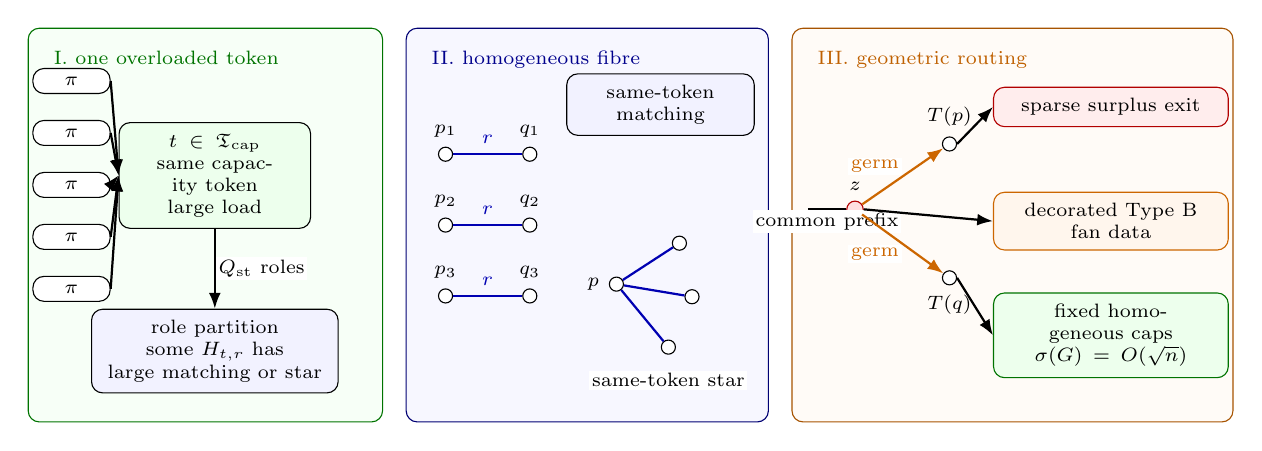
\begin{tikzpicture}[
pair/.style={rectangle,rounded corners,draw,fill=white,align=center,inner sep=3pt,minimum width=0.98cm},
token/.style={rectangle,rounded corners,draw,fill=green!7,align=center,inner sep=4pt,text width=2.15cm},
fiber/.style={rectangle,rounded corners,draw,fill=blue!5,align=center,inner sep=4pt,text width=2.85cm},
outcome/.style={rectangle,rounded corners,draw,fill=black!2,align=center,inner sep=4pt,text width=2.85cm},
exitbox/.style={rectangle,rounded corners,draw=red!70!black,fill=red!7,align=center,inner sep=4pt,text width=2.70cm},
fanbox/.style={rectangle,rounded corners,draw=orange!80!black,fill=orange!7,align=center,inner sep=4pt,text width=2.70cm},
capbox/.style={rectangle,rounded corners,draw=green!45!black,fill=green!7,align=center,inner sep=4pt,text width=2.70cm},
vtx/.style={circle,draw,fill=white,inner sep=1.8pt},
sep/.style={circle,draw=red!70!black,fill=red!12,inner sep=2.1pt},
arr/.style={-{Latex[length=2mm]},thick},
every node/.style={font=\scriptsize}
]
\draw[rounded corners,fill=green!3,draw=green!45!black] (-7.55,-2.45) rectangle (-3.05,2.55);
\draw[rounded corners,fill=blue!3,draw=blue!45!black] (-2.75,-2.45) rectangle (1.85,2.55);
\draw[rounded corners,fill=orange!3,draw=orange!65!black] (2.15,-2.45) rectangle (7.75,2.55);
\node[anchor=north west,green!45!black] at (-7.35,2.38) {I. one overloaded token};
\node[anchor=north west,blue!55!black] at (-2.55,2.38) {II. homogeneous fibre};
\node[anchor=north west,orange!75!black] at (2.35,2.38) {III. geometric routing};

\node[token] (t) at (-5.18,0.68) {$t\in\mathfrak T_{\rm cap}$\\same capacity token\\large load};
\foreach \name/\y in {pi1/1.88,pi2/1.22,pi3/0.56,pi4/-0.10,pi5/-0.76} {
  \node[pair] (\name) at (-7.00,\y) {$\pi$};
  \draw[arr] (\name.east)--(t.west);
}
\node[fiber] (role) at (-5.18,-1.55) {role partition\\some \(H_{t,r}\) has\\large matching or star};
\draw[arr] (t.south)--node[right,fill=white,inner sep=1pt] {$Q_{\rm st}$ roles} (role.north);

\node[vtx,label=above:$p_1$] (p1) at (-2.25,0.95) {};
\node[vtx,label=above:$q_1$] (q1) at (-1.18,0.95) {};
\node[vtx,label=above:$p_2$] (p2) at (-2.25,0.05) {};
\node[vtx,label=above:$q_2$] (q2) at (-1.18,0.05) {};
\node[vtx,label=above:$p_3$] (p3) at (-2.25,-0.85) {};
\node[vtx,label=above:$q_3$] (q3) at (-1.18,-0.85) {};
\draw[thick,blue!70!black] (p1)--node[above] {$r$}(q1);
\draw[thick,blue!70!black] (p2)--node[above] {$r$}(q2);
\draw[thick,blue!70!black] (p3)--node[above] {$r$}(q3);
\node[fiber,text width=2.10cm] (ms) at (0.48,1.58) {same-token matching};
\node[vtx,label=left:$p$] (s0) at (-0.08,-0.70) {};
\node[vtx] (s1) at (0.72,-0.18) {};
\node[vtx] (s2) at (0.88,-0.86) {};
\node[vtx] (s3) at (0.58,-1.50) {};
\draw[thick,blue!70!black] (s0)--(s1);
\draw[thick,blue!70!black] (s0)--(s2);
\draw[thick,blue!70!black] (s0)--(s3);
\node[anchor=center,fill=white,inner sep=1pt] at (0.58,-1.92) {same-token star};

\node[sep,label=above:$z$] (z) at (2.95,0.25) {};
\node[vtx,label=above:$T(p)$] (tp) at (4.15,1.08) {};
\node[vtx,label=below:$T(q)$] (tq) at (4.15,-0.62) {};
\draw[thick] (2.35,0.25)--node[below,fill=white,inner sep=1pt] {common prefix} (z);
\draw[arr,orange!80!black] (z)--node[above left,fill=white,inner sep=1pt] {germ} (tp);
\draw[arr,orange!80!black] (z)--node[below left,fill=white,inner sep=1pt] {germ} (tq);
\node[exitbox] (exit) at (6.20,1.55) {sparse surplus exit};
\node[fanbox] (fan) at (6.20,0.10) {decorated Type B\\fan data};
\node[capbox] (caps) at (6.20,-1.35) {fixed homogeneous caps\\\(\sigma(G)=O(\sqrt n)\)};
\draw[arr] (tp.east)--(exit.west);
\draw[arr] (z.east)--(fan.west);
\draw[arr] (tq.east)--(caps.west);
\end{tikzpicture}%
}
\caption[Visual definition of the homogeneous same-token bottleneck]{Visual definition of the homogeneous same-token bottleneck.  Panel I shows blocked active surplus pairs assigned by the capacity-token map to one overloaded token \(t\in\mathfrak T_{\rm cap}\).  The role partition of the fibre over \(t\) produces a role \(r\) for which the same-token role graph \(H_{t,r}\) contains a large matching or a large star.  Panel II displays the two possible homogeneous patterns: every shown edge has the same token \(t\) and the same role \(r\).  Panel III shows the geometric routing of two selected demands from the same homogeneous pattern.  Parallel routing germs give one of the quotient, compression, or delocalization exits already included among the sparse surplus exits.  If the germs first separate at a high-degree vertex \(z\), the separated tails form decorated Type B handoff fan data.  When neither a sparse surplus exit nor Type B fan data remains, all three token classes have fixed homogeneous caps, and \cref{cor:homogeneous-same-token-caps-close} gives \(\sigma(G)=O(\sqrt n)\).}
\label{fig:same-token-bottleneck-gadget}
\end{figure}

\begin{remark}[Exact surplus frontier]\label[remark]{rem:surplus-pair-sharp-frontier}
The sparse surplus bookkeeping has no disjointness loss.  The active family is
\(\mathcal A_0=\mathcal P_{\rm exc}\) by
\cref{lem:surviving-active-family}.  Free pairs are charged by
\cref{prop:sparse-entropy-sandwich-with-blockers}.  Blocked pairs are assigned a
canonical blocker and then one capacity token by
\cref{def:capacity-token-ledger}.  The token fibres partition the blocked-pair
set by \cref{lem:token-ledger-no-overcount}.  Therefore any attempted
non-near-cubic surplus survivor must first pass through one of the six subtype
loads in \cref{thm:sharp-surplus-overload-audit}, grouped into the three
diagram classes \(W=\{RW,WW\}\), \(R=\{R\}\), and \(P=\{V,I,P\}\).  A large
load in any one of those fibres is not terminal:
\cref{thm:homogeneous-overload-geometric-closure} routes it to a sparse surplus
exit, to Type B fan data, or to the fixed homogeneous caps that imply the
near-cubic spine.
\end{remark}

\begin{proposition}[Non-near-cubic sparse-pressure routing]\label[proposition]{prop:nonnear-cubic-sharp-overload-routing}
Let \(G\) be a lexicographically minimal counterexample that reaches node
\([18]\).  If \(G\) survives the sparse surplus exits, then the exact
sparse-pressure audit has only the following outcomes:
\begin{enumerate}[label=(\alph*), leftmargin=2.2em]
\item \(G\) satisfies the near-cubic spine estimate
\(\sigma(G)=O(\sqrt n)\);
\item a sparse surplus exit occurs; or
\item a role-homogeneous same-token bottleneck produces decorated Type B fan
data and is routed to the Type B fan ledger.
\end{enumerate}
In particular, the window-incidence, remainder-surplus, and primitive-carrier
same-token classes are not terminal non-near-cubic leaves.
\end{proposition}

\begin{proof}
If a sparse surplus exit occurs, there is nothing to route.  Otherwise
\cref{lem:surviving-active-family} gives
\(\mathcal A_0=\mathcal P_{\rm exc}\), and
\cref{prop:sparse-entropy-sandwich-with-blockers} supplies the free-pair
entropy bound used in \(N_*(G)\).  The blocked-pair ledger and token ledger are
exact by
\cref{lem:canonical-blocker-ledger-no-overcount,lem:token-ledger-no-overcount}.

Apply \cref{thm:homogeneous-overload-geometric-closure}.  If no homogeneous
same-token pattern reaches size \(L_{\rm geom}\), the fixed caps
\(L_W=L_R=L_P=L_{\rm geom}\) hold and
\cref{cor:homogeneous-same-token-caps-close} gives
\(\sigma(G)=O(\sqrt n)\).  If such a pattern exists, then
\cref{lem:same-token-bottleneck-routing} gives either a sparse surplus exit or
decorated Type B handoff data.  The subtype identity in
\cref{thm:sharp-surplus-overload-audit} records where the load came from:
\(RW\) and \(WW\) are window-incidence loads, \(R\) is a remainder-surplus
load, and \(V,I,P\) are primitive-carrier loads.  In all cases the load is
either closed, routed to Type B, or bounded by the fixed cap that yields the
near-cubic estimate.
\end{proof}


\subsection{Boundaried atoms, target-complete quotients, and replacement}

\begin{definition}[Boundaried graph and gluing]\label[definition]{def:boundaried-gluing}
Let $T$ be a finite label set.  A $T$-boundaried graph is a graph $X$ together with an injective labelling of a subset $\bd X\subseteq V(X)$ by $T$.  The vertices in $\bd X$ are boundary vertices; all others are internal.  If $X$ and $Y$ are $T$-boundaried graphs with disjoint internal vertex sets, their gluing is denoted
\[
X\oplus_T Y,
\]
and is obtained by identifying equally labelled boundary vertices and taking the union of edges.
\end{definition}

\begin{definition}[Atom]\label[definition]{def:atom}
An \emph{atom} of $G$ is a connected $T$-boundaried subgraph $X$ occurring as one side of a decomposition $G=X\oplus_T Y$ along a boundary $T\subseteq V(G)$; the other side $Y$ is its \emph{context}.  The atom is \emph{proper} if $X\ne G$.  The replacement and uncompressibility arguments of this section quantify over proper atoms.
\end{definition}

\begin{definition}[Boundary degree profile]\label[definition]{def:boundary-degree-profile}
Let $X$ be a $T$-boundaried graph.  For $t\in T$, let $v_t$ be the boundary vertex of $X$ labelled by $t$.  The boundary degree profile of $X$ is the vector
\[
\mathbf d_\partial(X)=(d_X(v_t))_{t\in T}.
\]
All target-response states in this paper are taken fibrewise over $\mathbf d_\partial$.  In particular, two boundaried states with different boundary degree profiles are never eligible to be identified by a target-complete quotient.
\end{definition}

\begin{definition}[Obstruction profile]\label[definition]{def:obstruction-profile}
For a $T$-boundaried graph $X$, define its target obstruction profile
\[
\profile_T(X)=\{Y\in\Ctx_T:X\oplus_TY\text{ contains a power-of-two cycle}\},
\]
where $\Ctx_T$ is the class of finite $T$-boundaried contexts that can be glued to $X$.  If $X'$ and $X$ are $T$-boundaried graphs, write
\[
X'\preceq_T X
\]
if
\[
\profile_T(X')\subseteq\profile_T(X).
\]
Thus $X'$ is at most as obstructing as $X$.
\end{definition}

\begin{definition}[Target-complete quotient]\label[definition]{def:target-complete-quotient}
Let $X$ be a $T$-boundaried atom, and let $\mathcal R(X)$ be a collection of local target-response coordinates of $X$, such as terminal trace lengths, edge-rooted Mersenne-return tests, curvature-flatness tests, boundary degree data, and other marked response data.
A quotient of $\mathcal R(X)$ is \emph{target-complete} if every identification made by the quotient preserves both:
\begin{enumerate}[label=(\alph*)]
\item the boundary degree profile $\mathbf d_\partial(X)$; and
\item the target predicate after gluing $X$ to every $T$-boundaried context.
\end{enumerate}
Thus two coordinates may be identified only inside a fixed boundary-degree fibre and only when no context $Y\in\Ctx_T$ creates a power-of-two cycle from one coordinate and not from the other.  An identification failing this context-universal test is \emph{target-defective}.
\end{definition}

\begin{lemma}[Composition of target-complete quotients]\label[lemma]{lem:target-complete-quotient-composition}
Let
\[
\rho\longrightarrow Q\longrightarrow Q'
\]
be boundary-degree-preserving response quotients tested against the same class of
compatible boundaried contexts.  If both displayed quotients are
target-complete, then the composite quotient \(\rho\to Q'\) is target-complete.
Consequently, if \(\rho\to Q\) is target-complete and the composite
\(\rho\to Q'\) is not target-complete, then \(Q\to Q'\) is not
target-complete.  Moreover, any compatible context that distinguishes a
realization of \(Q'\) from the state \(Q\) also distinguishes that realization
from \(\rho\) after composing with the target-complete quotient \(\rho\to Q\).
\end{lemma}

\begin{proof}
Fix a compatible outside context \(Y\).  Target-completeness of \(Q\to Q'\)
says that every realization of \(Q'\), glued to \(Y\), has the same target
predicate as the corresponding \(Q\)-state.  Target-completeness of
\(\rho\to Q\) says that the \(Q\)-state, glued to \(Y\), has the same target
predicate as \(\rho\).  Hence every realization of \(Q'\) has the same target
predicate as \(\rho\) after gluing to \(Y\).  Since \(Y\) was arbitrary, the
composite is target-complete.  The contrapositive gives the second assertion.
The last assertion is the same transitivity statement applied to a fixed
distinguishing context.
\end{proof}

\begin{definition}[Declared response-coordinate signature]\label[definition]{def:declared-coordinate-signature}
The response-coordinate signature used in the proof is fixed once and for all.
For a $T$-boundaried support $X$, a declared coordinate is a tuple
\[
(k,\iota,\supp_X(r),\operatorname{val}_X(r)),
\]
where $k$ is its kind, $\iota$ is its label, $\supp_X(r)$ is a finite set of
vertices, edges, boundary incidences, paths, or windows of $X$, and
\(\operatorname{val}_X(r)\) is the corresponding value in the embedded support.  The declared
coordinates are generated by the following clauses.
\begin{enumerate}[label=(D\arabic*), leftmargin=2.2em]
\item boundary-degree entries at labelled boundary vertices;
\item edge-rooted return data, completion-port data, first-entry receivers,
connector lengths, receiver-entry channels, and the corresponding Mersenne
return tests;
\item induced-$P_{13}$ window labels, legal-label relations, packed-window
incidences, and cross-window incidence data;
\item raw curvature coordinates indexed by internal length-two wedges;
\item Type A trace data: canonical traces, trace-incidence coordinates,
connector-band constraints, cross-port theta constraints, silent-basin response
coordinates, carrier restrictions, and their labelled subcoordinates;
\item Type B fan and bridge data: fan centers, fan-safe pairs, certificate
labels, closed fan-window pairs, hybrid incidence entries, candidate ledger
entries, overlap demands, decorated handoff fan response coordinates, and
decorated handoff-arm coordinates;
\item sparse surplus data: selected surplus ports, canonical port returns,
open-port suppression paths, triangular-port response triangles, and sparse
surplus-pair response coordinates;
\item finite products, labelled copies, restrictions, and quotient images of
coordinates already generated in clauses (D1)--(D7), with support equal to the
union of the supports of the entries used.
\end{enumerate}
No other local response coordinate is available to a quotient.  Whenever a later
definition names a coordinate family, it names the subfamily generated by this
signature with the displayed labels.  In particular, a phrase such as
``needed to evaluate a return'' means that the relevant port, first-entry
incidence, connector endpoint, channel, window, or boundary incidence is a
member of the declared support specified by the corresponding clause above.
\end{definition}

\begin{definition}[Exact response profile]\label[definition]{def:exact-response-profile}
Let $X$ be a $T$-boundaried support.  Let
$\mathfrak S_T(X)$ be the finite labelled family of coordinates generated on
$X$ by \cref{def:declared-coordinate-signature}.  The \emph{exact response
profile} of $X$ is
\[
\rho_T^{\rm ex}(X)=
\bigl(\mathbf d_\partial(X),\profile_T(X),\mathcal R_T^{\rm ex}(X)\bigr),
\]
where $\mathcal R_T^{\rm ex}(X)=\mathfrak S_T(X)$, including the raw curvature
coordinates carried by $X$ when they are present.  The profile is exact in the
following sense: two distinct coordinate labels remain distinct entries of
$\mathcal R_T^{\rm ex}(X)$ even if their numerical values in the embedded graph
coincide.

A quotient
\[
q:\rho_T^{\rm ex}(X)\longrightarrow Q
\]
is \emph{label-injective on a subfamily} $\mathcal A\subseteq
\mathcal R_T^{\rm ex}(X)$ if every coordinate of $\mathcal A$ is retained by
$q$ and
\[
q(a)=q(b)\quad\text{with }a,b\in\mathcal A
\qquad\Longrightarrow\qquad a=b .
\]
It is \emph{rank-reducing} on $\mathcal A$ if it is not label-injective on
\(\mathcal A\).
\end{definition}

\begin{definition}[Proper representative of an exact-profile quotient]\label[definition]{def:proper-quotient-representative}
Let \(G=X\oplus_TY\), where \(X\subsetneq G\) is a proper \(T\)-boundaried
support, and let
\[
q:\rho_T^{\rm ex}(X)\to Q
\]
be a quotient of its exact profile.  A \(T\)-boundaried graph \(X'\)
\emph{properly represents} \(q\) if there is a quotient
\[
q_{X'}:\rho_T^{\rm ex}(X')\to Q
\]
with the following properties.
\begin{enumerate}[label=(\alph*), leftmargin=2.2em]
\item \(\profile_T(X')\subseteq\profile_T(X)\).
\item \(\mathbf d_\partial(X')=\mathbf d_\partial(X)\).
\item \(X'\) contains no internal power-of-two cycle.
\item Every internal vertex of \(X'\) has degree at least \(3\).
\item Every labelled coordinate of \(Q\) is the image under \(q_{X'}\) of a
coordinate generated by \cref{def:declared-coordinate-signature}, and the
quotient relations among the coordinates under discussion are the same as
those imposed by \(q\).
\end{enumerate}
The representative is \emph{strictly smaller} if \(X'\) is smaller than \(X\)
in the lexicographic order used for the minimal counterexample.
\end{definition}

\begin{definition}[Closed representative of an exact-profile quotient]\label[definition]{def:closed-quotient-representative}
Let
\[
q:\rho_\varnothing^{\rm ex}(G)\to Q
\]
be a quotient of the closed exact profile.  A finite simple closed graph $H$
\emph{represents} $q$ if there is a quotient
\[
q_H:\rho_\varnothing^{\rm ex}(H)\to Q
\]
with the following properties.
\begin{enumerate}[label=(\alph*), leftmargin=2.2em]
\item The obstruction-profile component of $q_H$ is no larger than that of $G$:
\[
\profile_\varnothing(H)\subseteq\profile_\varnothing(G).
\]
\item The boundary-degree component is the empty boundary profile.
\item Every labelled coordinate of $Q$ is the image under $q_H$ of a coordinate
generated by the declared signature of \cref{def:declared-coordinate-signature},
and the quotient relations among raw curvature coordinates recorded in $Q$ are
the same quotient relations as those imposed by $q$.
\end{enumerate}
The representative is \emph{strictly smaller} when $H$ is smaller than $G$ in
the lexicographic minimality order.  It is \emph{admissible closed} when, in
addition, $\delta(H)\ge3$.
\end{definition}

\begin{definition}[Admissible rank quotient]\label[definition]{def:admissible-rank-quotient}
Let $\mathcal A$ be a family of declared response coordinates carried by a
connected support $X\subseteq G$, and put
\[
T=\{v\in V(X):v\text{ is incident with an edge of }G-X\}.
\]
An \emph{admissible rank quotient} for $\mathcal A$ is a quotient
\[
q:\rho_T^{\rm ex}(X)\longrightarrow Q
\]
which preserves the boundary degree profile and is target-complete against all
$T$-boundaried contexts in the sense above.

If \(X\subsetneq G\), then a rank-reducing admissible quotient must be
represented by a strictly smaller proper representative in the sense of
\cref{def:proper-quotient-representative}.  Equivalently, a target-complete
proper-support correlation that has no smaller graph representative is not an
admissible rank reduction; it is only an abstract identification of labels and
does not reduce the graph-realizable target rank used in this proof.

If $T=\varnothing$ and $X=G$, the quotient is evaluated in the closed exact
profile
$\rho_\varnothing^{\rm ex}(G)$.  In that closed case, absence of an outside
context is not an identification rule: an admissible rank quotient must be
label-injective on the declared coordinates under discussion unless it is represented by a
strictly smaller admissible closed representative in the sense of
\cref{def:closed-quotient-representative}.

Thus the empty-boundary profile may record exact global information, but exact
global information does not collapse two labelled response coordinates.  A
closed non-injective quotient can affect target rank only when it supplies a
strictly smaller closed representative; such a representative would be a
smaller counterexample if the target predicate is still false.
\end{definition}

\begin{definition}[Functional rank quotient]\label[definition]{def:functional-rank-quotient}
Let \(q:\rho_T^{\rm ex}(X)\to Q\) be an admissible rank quotient for a finite
coordinate family \(\mathcal A\).  The quotient \(q\) is \emph{functional on}
\(\mathcal A\) if the following rank axiom holds.  Whenever
\(\mathcal I\subseteq\mathcal A\) and \(a\in\mathcal A\setminus\mathcal I\)
are such that \(q\) is label-injective on \(\mathcal I\), but is not
label-injective on \(\mathcal I\cup\{a\}\), there is a finite subfamily
\(\mathcal B\subseteq\mathcal I\) and a function \(\phi\) on the realized
\(q\)-image vectors of \(\mathcal B\) such that
\[
q(a)=\phi\bigl((q(b))_{b\in\mathcal B}\bigr)
\]
for every realization of the exact response profile under \(q\).  If the
quotient sends \(a\) to a single quotient value, then \(\mathcal B=\varnothing\).
If the quotient identifies \(a\) with a coordinate \(b\in\mathcal I\), then
\(\mathcal B=\{b\}\) and \(\phi(q(b))=q(b)\).

The admissible quotient system used to compute target-rank consists only of
admissible rank quotients that are functional on the coordinate family under
discussion.
\end{definition}

\begin{remark}[Rank coordinates and entropy charge]\label[remark]{rem:rank-coordinate-entropy-interface}
The curvature target-rank \(r_\Omega\) is always computed from the declared
coordinates of the exact response profile and from admissible rank quotients in
the sense of
\cref{def:exact-response-profile,def:admissible-rank-quotient,def:functional-rank-quotient}.
Thus a rank coordinate contributes to the entropy count only when it remains a
labelled, independently target-testable coordinate after all admissible
quotients have been applied.  This is the interface used by
\cref{lem:independent-target-entropy,prop:two-budget}: raw curvature tests are
not counted twice, and an abstract identification that is not an admissible
rank quotient does not reduce \(r_\Omega\).
\end{remark}

\begin{lemma}[Boundary degree profiles cannot be quotient-merged]\label[lemma]{lem:degree-profile-fibres}
Let $X_1$ and $X_2$ be $T$-boundaried supports.  If
\[
\mathbf d_\partial(X_1)\ne \mathbf d_\partial(X_2),
\]
then no target-complete quotient identifies $X_1$ and $X_2$.
\end{lemma}

\begin{proof}
Condition~(a) in the definition of a target-complete quotient requires the
quotient to preserve the boundary degree profile.  If
\(\mathbf d_\partial(X_1)\ne\mathbf d_\partial(X_2)\), an identification of
\(X_1\) with \(X_2\) would identify two different boundary-degree profiles, so
it violates condition~(a).  Thus two supports lying in different
boundary-degree fibres are not eligible for identification, independently of
the context-universal target test in condition~(b).
\end{proof}

\begin{lemma}[Context-universality of target-complete identifications]\label[lemma]{lem:context-universality}
Let $X$ be a $T$-boundaried atom, and let $\mathcal R(X)$ be any collection of local target-response coordinates of $X$.  Suppose that two coordinates $r_1,r_2\in\mathcal R(X)$ are identified in a target-complete quotient of $X$.  Then $r_1$ and $r_2$ have the same target response against every $T$-boundaried context $Y$.

Equivalently, for every $Y\in\Ctx_T$, gluing $Y$ to $X$ cannot distinguish $r_1$ from $r_2$ by creating a power-of-two cycle in one case and not in the other.  Consequently any identification valid only for the actual outside context $G-X$, but not for all $T$-boundaried contexts, is target-defective.
\end{lemma}

\begin{proof}
This is precisely the meaning of target-completeness.  If some context $Y_0$ distinguished $r_1$ and $r_2$, then one of the two gluings would contain a power-of-two cycle and the other would not.  The quotient would fail to preserve the target predicate for $Y_0$ and therefore would not be target-complete.
\end{proof}

\begin{lemma}[Replacement lemma for boundaried atoms]\label[lemma]{lem:replacement}
Let $G=X\oplus_TY$, where $X$ is a proper atom of $G$.  Suppose there exists a $T$-boundaried graph $X'$ such that:
\begin{enumerate}[label=(\roman*)]
\item $X'\preceq_T X$;
\item $\mathbf d_\partial(X')=\mathbf d_\partial(X)$;
\item $X'$ contains no internal power-of-two cycle;
\item every internal vertex of $X'$ has degree at least $3$;
\item $X'$ is strictly smaller than $X$ in the same lexicographic order used for $G$.
\end{enumerate}
Then $G$ was not minimal.  Consequently no such replacement exists in $G$.
\end{lemma}

\begin{proof}
Form
\[
G'=X'\oplus_TY.
\]
Because $\mathbf d_\partial(X')=\mathbf d_\partial(X)$, every boundary vertex has the same final degree in $G'$ as it had in $G$.  Vertices of $Y$ are unchanged, and internal vertices of $X'$ have degree at least $3$ by hypothesis.  Hence $\delta(G')\ge3$.

We claim that $G'$ has no power-of-two cycle.  Let $C$ be a cycle of $G'$, and suppose for contradiction that its length is a power of two.  If $C$ is wholly contained in $Y$, then $C$ is also a cycle of $G$, contradicting that $G$ is a counterexample.  If $C$ is wholly contained in $X'$, then $C$ is an internal power-of-two cycle of $X'$, forbidden by hypothesis~(iii).  Otherwise $C$ uses internal vertices of both $X'$ and $Y$; since $X'$ and $Y$ meet only in the boundary $\bd$, the cycle $C$ lives in $G'=X'\oplus_TY$ and contains a power-of-two cycle, so by definition of the obstruction profile $Y\in\profile_T(X')$.  Hypothesis~(i) gives $X'\preceq_TX$, that is $\profile_T(X')\subseteq\profile_T(X)$, whence $Y\in\profile_T(X)$.  By definition this means $X\oplus_TY=G$ contains a power-of-two cycle, contradicting that $G$ is a counterexample.  Hence $G'$ has no power-of-two cycle.  Together with $\delta(G')\ge3$ and hypothesis~(v), $G'$ is a counterexample strictly smaller than $G$ in the lexicographic order, contradicting the minimality of $G$.
\end{proof}

\begin{definition}[Target-complete compression]\label[definition]{def:target-complete-compression}
Let $X$ be a proper atom.  A nontrivial target-complete compression of $X$ is a smaller $T$-boundaried representative $X'$ satisfying the hypotheses of \cref{lem:replacement}.  A quotient or identification of local response coordinates that is not target-complete is called a target-defective quotient.
\end{definition}

\begin{corollary}[Hereditary target-uncompressibility]\label[corollary]{cor:uncompressible}
No proper atom of $G$ admits a nontrivial target-complete compression.  Moreover, a non-target-complete identification cannot be used as a replacement that preserves the counterexample predicate: by definition of target completeness and \cref{lem:context-universality}, some outside context distinguishes the identified states by producing a power-of-two cycle from one and not from the other.
\end{corollary}

\begin{proof}
The first assertion is exactly \cref{lem:replacement}.  The second assertion is \cref{lem:context-universality}.
\end{proof}

\begin{figure}[t]
\centering
\resizebox{0.98\textwidth}{!}{%
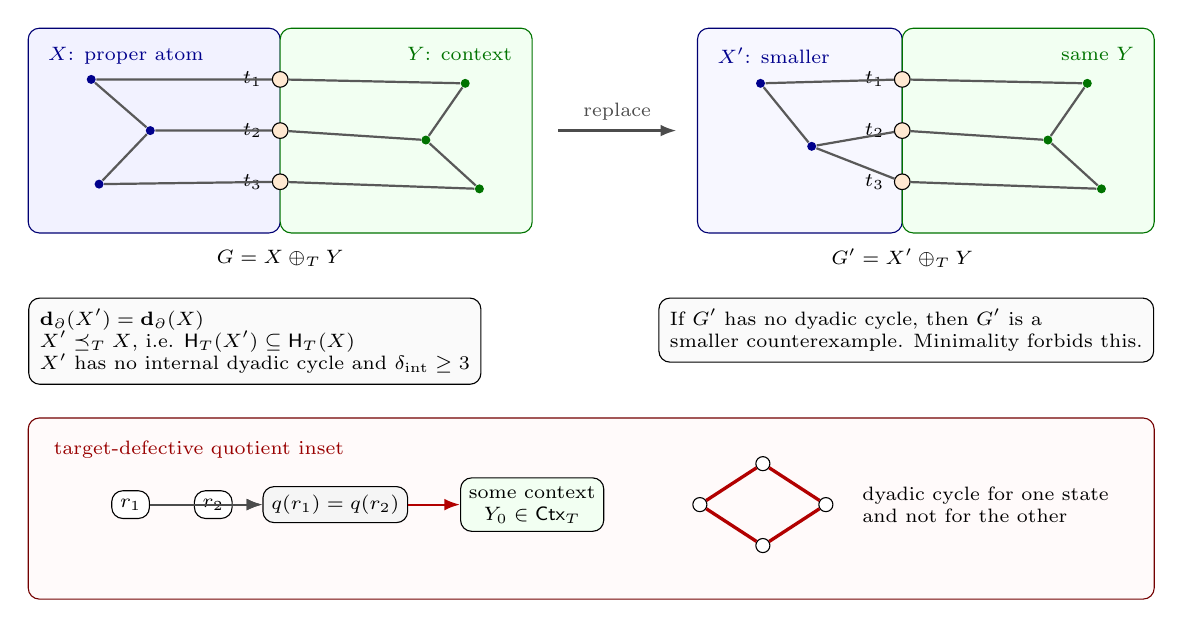
\begin{tikzpicture}[
vtx/.style={circle,draw,fill=white,inner sep=1.8pt},
bdv/.style={circle,draw=black,fill=orange!18,inner sep=2.0pt},
intx/.style={circle,fill=blue!55!black,inner sep=1.15pt},
inty/.style={circle,fill=green!45!black,inner sep=1.15pt},
edge/.style={thick,black!65},
arr/.style={-{Latex[length=2mm]},thick,black!70},
bad/.style={-{Latex[length=2mm]},thick,red!70!black},
box/.style={rectangle,rounded corners,draw,align=left,inner sep=4pt,fill=black!2},
smallbox/.style={rectangle,rounded corners,draw,align=center,inner sep=3pt,fill=white},
every node/.style={font=\scriptsize}
]
% Original gluing.
\draw[rounded corners,fill=blue!5,draw=blue!45!black] (-7.25,0.10) rectangle (-4.05,2.70);
\draw[rounded corners,fill=green!5,draw=green!45!black] (-4.05,0.10) rectangle (-0.85,2.70);
\node[anchor=north west,blue!55!black] at (-7.12,2.58) {$X$: proper atom};
\node[anchor=north east,green!45!black] at (-0.98,2.58) {$Y$: context};
\node[bdv,label=left:$t_1$] (b1) at (-4.05,2.05) {};
\node[bdv,label=left:$t_2$] (b2) at (-4.05,1.40) {};
\node[bdv,label=left:$t_3$] (b3) at (-4.05,0.75) {};
\node[intx] (x1) at (-6.45,2.05) {};
\node[intx] (x2) at (-5.70,1.40) {};
\node[intx] (x3) at (-6.35,0.72) {};
\draw[edge] (x1)--(x2)--(x3);
\draw[edge] (x1)--(b1) (x2)--(b2) (x3)--(b3);
\node[inty] (y1) at (-1.70,2.00) {};
\node[inty] (y2) at (-2.20,1.28) {};
\node[inty] (y3) at (-1.52,0.66) {};
\draw[edge] (b1)--(y1)--(y2)--(y3)--(b3);
\draw[edge] (b2)--(y2);
\node at (-4.05,-0.22) {$G=X\oplus_TY$};

% Replacement gluing.
\draw[arr] (-0.52,1.40)--node[above] {replace} (0.98,1.40);
\draw[rounded corners,fill=blue!3,draw=blue!45!black] (1.25,0.10) rectangle (3.85,2.70);
\draw[rounded corners,fill=green!5,draw=green!45!black] (3.85,0.10) rectangle (7.05,2.70);
\node[anchor=north west,blue!55!black] at (1.38,2.58) {$X'$: smaller};
\node[anchor=north east,green!45!black] at (6.92,2.58) {same \(Y\)};
\node[bdv,label=left:$t_1$] (bp1) at (3.85,2.05) {};
\node[bdv,label=left:$t_2$] (bp2) at (3.85,1.40) {};
\node[bdv,label=left:$t_3$] (bp3) at (3.85,0.75) {};
\node[intx] (xp1) at (2.05,2.00) {};
\node[intx] (xp2) at (2.70,1.20) {};
\draw[edge] (xp1)--(xp2);
\draw[edge] (xp1)--(bp1) (xp2)--(bp2) (xp2)--(bp3);
\node[inty] (yp1) at (6.20,2.00) {};
\node[inty] (yp2) at (5.70,1.28) {};
\node[inty] (yp3) at (6.38,0.66) {};
\draw[edge] (bp1)--(yp1)--(yp2)--(yp3)--(bp3);
\draw[edge] (bp2)--(yp2);
\node at (3.85,-0.22) {$G'=X'\oplus_TY$};

\node[box,anchor=north west] at (-7.25,-0.72)
{\(\mathbf d_\partial(X')=\mathbf d_\partial(X)\)\\
\(X'\preceq_T X\), i.e. \(\profile_T(X')\subseteq\profile_T(X)\)\\
\(X'\) has no internal dyadic cycle and \(\delta_{\rm int}\ge3\)};
\node[box,anchor=north east] at (7.05,-0.72)
{If \(G'\) has no dyadic cycle, then \(G'\) is a\\
smaller counterexample.  Minimality forbids this.};

% Target-defective quotient inset.
\draw[rounded corners,fill=red!2,draw=red!45!black] (-7.25,-4.55) rectangle (7.05,-2.25);
\node[anchor=north west,red!60!black] at (-7.05,-2.42) {target-defective quotient inset};
\node[smallbox] (r1) at (-5.95,-3.35) {$r_1$};
\node[smallbox] (r2) at (-4.90,-3.35) {$r_2$};
\node[smallbox,fill=black!4] (q) at (-3.35,-3.35) {$q(r_1)=q(r_2)$};
\draw[arr] (r1)--(q);
\draw[arr] (r2)--(q);
\node[smallbox,fill=green!5] (ctx) at (-0.85,-3.35) {some context\\ \(Y_0\in\Ctx_T\)};
\draw[bad] (q)--(ctx);
\node[vtx] (cu) at (1.28,-3.35) {};
\node[vtx] (cv) at (2.08,-2.83) {};
\node[vtx] (cw) at (2.88,-3.35) {};
\node[vtx] (cz) at (2.08,-3.87) {};
\draw[red!70!black,very thick] (cu)--(cv)--(cw)--(cz)--(cu);
\node[anchor=west,align=left] at (3.22,-3.35) {dyadic cycle for one state\\ and not for the other};
\end{tikzpicture}%
}
\caption[Visual definition of boundaried replacement]{Visual definition of boundaried replacement and target-completeness.  The left panel shows a proper atom \(X\) glued to its context \(Y\) along the labelled boundary \(T=\{t_1,t_2,t_3\}\), whose orange vertices are identified in \(G=X\oplus_TY\).  The right panel shows a smaller \(T\)-boundaried representative \(X'\) glued to the same context.  The hypotheses \(\mathbf d_\partial(X')=\mathbf d_\partial(X)\) and \(X'\preceq_T X\) mean that the boundary degrees are in the same fibre and every context obstructed by \(X'\) is also obstructed by \(X\).  If \(X'\) has no internal dyadic cycle and all internal vertices keep degree at least \(3\), then \(X'\oplus_TY\) would be a smaller counterexample, contradicting minimality.  The lower inset records the complementary failure mode: identifying two response coordinates \(r_1,r_2\) is target-defective when some context \(Y_0\) creates a dyadic cycle for one state and not for the other, so the quotient is not target-complete.}
\label{fig:boundaried-replacement-gadget}
\end{figure}

\begin{definition}[Target tester and independent target coordinates]\label[definition]{def:target-rank}
Let $X$ be a $T$-boundaried graph.  A target tester for a local coordinate $r$ of $X$ is a $T$-boundaried context $Y_r$ such that the gluing $X\oplus_TY_r$ contains a power-of-two cycle if and only if the coordinate $r$ takes the obstructing value, while all other coordinates under discussion are held fixed.

A finite family of local coordinates $\mathcal I=\{r_1,\ldots,r_k\}$ is \emph{independently target-testable} if its target responses realize $2^k$ distinct target-complete states; equivalently, for every subset $J\subseteq\{1,\ldots,k\}$ there is a target-complete state of the atom in which precisely the coordinates indexed by $J$ are obstructing.  The \emph{target rank} of a coordinate family is the maximum size of an independently target-testable subfamily.
\end{definition}

\begin{lemma}[Independent target coordinates consume skeleton entropy]\label[lemma]{lem:independent-target-entropy}
Let $\mathcal I$ be an independently target-testable family of size $k$ arising canonically from graphs in a labelled graph class $\mathcal G$.  Then
\[
2^k\le |\mathcal G|.
\]
In particular,
\[
k\le \log_2|\mathcal G|.
\]
\end{lemma}

\begin{proof}
By independent target-testability, the family $\mathcal I$ realizes $2^k$ distinct target-complete states.  If two distinct such states came from the same labelled graph, the canonical target-response map of that graph would be identical in both cases, contradiction.  Hence the number of states is at most the number of labelled graphs in the ambient class.
\end{proof}

\paragraph{Framework branch table.}
The target-algebra and replacement section instantiates the framework branch
table as follows.
\begin{longtable}{L{0.13\textwidth} L{0.19\textwidth} L{0.14\textwidth} L{0.14\textwidth} L{0.17\textwidth} L{0.17\textwidth}}
\FrameworkBranchTableHeader
Target hit
&
An edge-rooted Mersenne return is present.
&
No residual demand remains.
&
The target predicate.
&
Not applicable.
&
It is a dyadic cycle by \cref{lem:return-equivalence}.
\\
\addlinespace
Deletion
&
Deleting an edge would leave a smaller counterexample.
&
The deleted edge.
&
Lexicographic minimality.
&
One edge at a time.
&
Contradicts \cref{lem:deletion-critical}.
\\
\addlinespace
Boundary fibre
&
A quotient identifies supports with different boundary-degree profiles.
&
The boundary-degree discrepancy.
&
The fixed boundary fibre.
&
One canonical boundary profile per fibre.
&
Forbidden by \cref{lem:degree-profile-fibres}.
\\
\addlinespace
Target defect
&
An outside context distinguishes two identified coordinates.
&
A target-defective quotient.
&
The defect account attached to its declared support.
&
The finite declared coordinate signature.
&
Routed by \cref{lem:context-universality}.
\\
\addlinespace
Compression
&
A proper atom has a smaller target-complete representative.
&
The proper support size.
&
Minimality.
&
One replacement per proper atom.
&
Contradicts \cref{lem:replacement,cor:uncompressible}.
\\
\addlinespace
Entropy coordinate
&
Independent target coordinates are realized.
&
The number of target states.
&
The labelled skeleton count.
&
The canonical state map.
&
Bounded by \cref{lem:independent-target-entropy}.
\\
\bottomrule
\end{longtable}

\section{Sparse rank parameters}

Define
\[
\beta=m-n+1,
\qquad
\lambda=2n-3-m.
\]
Then
\[
\boxed{\beta+\lambda=n-2.}
\]
Define the surplus above cubic degree
\[
\sigma=\sum_{v\in V(G)}(d(v)-3)=2m-3n.
\]
Then
\[
\boxed{\beta=\frac n2+1+\frac{\sigma}{2}},
\qquad
\boxed{\lambda=\frac n2-3-\frac{\sigma}{2}}.
\]
The sparse skeleton entropy in the sparse ($\lambda$-parametrized) branch is
\[
B_{\mathrm{skel}}(n,\lambda)=\log_2\binom{\binom n2}{2n-3-\lambda}.
\]

\begin{definition}[Near-cubic spine hypothesis]\label[definition]{def:near-cubic-spine}
The \emph{near-cubic spine hypothesis} is the assertion that every
lexicographically minimal counterexample surviving to the entropy/net-charge
spine satisfies
\[
m=\frac32 n+O(\sqrt n),
\qquad
\sigma(G)=O(\sqrt n).
\]
Equivalently, the global surplus is \(o(n)\), and the labelled skeleton budget
available to the spine is
\[
\frac32 n\log_2 n+o(n\log n).
\]
In the final proof, this estimate is supplied by
\cref{prop:nonnear-cubic-sharp-overload-routing} before either the normalized
skeleton budget \(1.5\,n\log_2 n+o(n\log n)\) or the fan-mass estimate
\(\sigma(G)=o(|R|)\) is invoked.  When a later local lemma states
\cref{def:near-cubic-spine} among its hypotheses, that line records the branch
state needed for the normalized estimate, not an additional global assumption.
The local surplus bookkeeping relevant to deriving this hypothesis is recorded
in \cref{def:surplus-ports,def:fan-compatible-open-ports}.  The
degree-greater-than-four part is separated by
\cref{cor:heavy-center-local-dichotomy} and \cref{rem:degree-greater-four-leaf};
the degree-four local activation is \cref{cor:degree-four-local-activation};
and the non-near-cubic surplus branch is routed by the exact token ledger and
the same-token bottleneck closure
\cref{lem:same-token-bottleneck-routing,thm:homogeneous-overload-geometric-closure,prop:nonnear-cubic-sharp-overload-routing}.
\end{definition}

The following lemmas make explicit why this is a safe \emph{upper} bound on every degree of freedom available to a near-cubic graph.  The entropy budget is not an encoding assumption: it is merely the number of labelled adjacency matrices in the ambient class.

\begin{lemma}[Labelled skeleton budget dominates all auxiliary data]\label[lemma]{lem:skeleton-dominates}
Fix $n$ and $m$.  Let $\mathcal G_{n,m}$ be the set of all finite simple labelled graphs on vertex set $[n]$ with exactly $m$ edges.  Then
\[
|\mathcal G_{n,m}|=\binom{\binom n2}{m}.
\]
Consequently, if a collection of target-complete states is assigned canonically to graphs in $\mathcal G_{n,m}$, then the number of realized states is at most
\[
\binom{\binom n2}{m}.
\]
In particular, any target-complete response algebra that realizes more than
\[
2^{B_{\mathrm{skel}}(n,\lambda)}
\]
states among graphs with $m=2n-3-\lambda$ edges cannot be realized by such graphs.
\end{lemma}

\begin{proof}
A labelled simple graph on $[n]$ is uniquely determined by its edge set, a subset of the $\binom n2$ possible unordered pairs.  Thus the number with $m$ edges is exactly $\binom{\binom n2}{m}$.

All auxiliary objects used in the proof---a maximal induced-$P_{13}$ packing, atom decomposition, boundary profiles, spanning-tree choices, and curvature-response data---are functions of the labelled adjacency matrix once a deterministic tie-breaking rule is fixed.  We fix throughout the lexicographically first object among all objects with the required extremal property.  Thus no auxiliary structure supplies independent degrees of freedom beyond the adjacency matrix.  Hence the number of realized target-complete states is bounded by the number of labelled skeletons.
\end{proof}

\begin{lemma}[Variable edge-count budget]\label[lemma]{lem:variable-edge-budget}
Let $I\subseteq\{0,1,\ldots,\binom n2\}$ be any interval of possible edge counts.  Then the number of labelled graphs on $[n]$ whose edge count lies in $I$ is at most
\[
|I|\max_{m\in I}\binom{\binom n2}{m}.
\]
Consequently the logarithmic budget differs from the largest fixed-$m$ budget by at most $\log_2 |I|\le \log_2 n^2=2\log_2 n$ whenever $I$ has length at most $n^2$.
\end{lemma}

\begin{proof}
The graphs with different edge counts are disjoint, so the total number is the sum of $\binom{\binom n2}{m}$ over $m\in I$.  This sum is at most $|I|$ times its largest summand.  Taking logarithms gives the claim.
\end{proof}

\begin{lemma}[Near-cubic specialization of the skeleton budget]\label[lemma]{lem:near-cubic-budget}
Suppose
\[
m=\frac32 n+O(\sqrt n).
\]
Then
\[
\log_2\binom{\binom n2}{m}
=\frac32 n\log_2 n+O(n)+O(\sqrt n\log n).
\]
In particular,
\[
B_{\mathrm{skel}}(n,\lambda)=\frac32 n\log_2 n+o(n\log n)
\]
in the near-cubic branch.
\end{lemma}

\begin{proof}
Let $N=\binom n2$.  The standard binomial estimate
\[
\binom Nm\le \left(\frac{eN}{m}\right)^m
\]
gives
\[
\log_2\binom Nm\le m\log_2\left(\frac{eN}{m}\right).
\]
If $m=\frac32n+O(\sqrt n)$, then $N=\frac12n^2+O(n)$ and therefore
\[
\frac{eN}{m}=\Theta(n).
\]
Hence
\[
\log_2\binom Nm\le \left(\frac32 n+O(\sqrt n)\right)(\log_2 n+O(1))
=\frac32 n\log_2 n+O(n)+O(\sqrt n\log n).
\]
The matching lower asymptotic is not needed in the proof; the displayed upper bound is what is used.  Since $O(n)+O(\sqrt n\log n)=o(n\log n)$, the final statement follows.
\end{proof}

\begin{remark}[Scope of the near-cubic budget]\label[remark]{rem:near-cubic-budget-scope}
\Cref{lem:near-cubic-budget} is the conversion step from
\(m=\frac32n+O(\sqrt n)\) to the entropy budget used later.  The surplus-token
routing branch supplies this edge-count estimate before the lemma is invoked in
the final proof.
\end{remark}

\begin{remark}[Robustness of the skeleton budget]\label[remark]{rem:budget-robustness}
The budget counts all labelled simple graphs with the given edge count.  The near-cubic, minimality, atom, curvature, and target constraints only restrict this set.  Automorphisms only reduce the number of unlabelled graphs, so labelled counting is an overcount.  Degree sequences are not additional data: they are determined by the edge set.  Likewise, packings, atoms, trees, and profiles are treated canonically and are deterministic functions of the graph.  Thus one cannot obtain extra graph-theoretic degrees of freedom by varying these auxiliary choices; doing so would only count the same labelled graph multiple times.
\end{remark}

\begin{lemma}[State-count comparison]\label[lemma]{lem:state-count-comparison}
Let $\mathcal S$ be a family of target-complete states realized by labelled graphs in a class $\mathcal G$.  If the state map is canonical, then
\[
|\mathcal S|\le |\mathcal G|.
\]
Equivalently, if the proof establishes $K$ independently testable Boolean target coordinates, so that at least $2^K$ target-complete states are realized, then necessarily
\[
K\le \log_2 |\mathcal G|.
\]
\end{lemma}

\begin{proof}
The canonical state map sends each graph to one state.  Therefore the number of realized states cannot exceed the number of graphs.  If $K$ independent Boolean target coordinates are realized, they give at least $2^K$ distinct target-complete states.  Hence $2^K\le |\mathcal G|$ and the logarithmic inequality follows.
\end{proof}

\paragraph{Framework branch table.}
The sparse-rank section supplies the global budget branch table.
\begin{longtable}{L{0.13\textwidth} L{0.19\textwidth} L{0.14\textwidth} L{0.14\textwidth} L{0.17\textwidth} L{0.17\textwidth}}
\FrameworkBranchTableHeader
Fixed edge count
&
States are assigned to a fixed-\(m\) labelled graph class.
&
Target-complete states.
&
Labelled edge sets.
&
One canonical state per labelled graph.
&
Bounded by \cref{lem:skeleton-dominates}.
\\
\addlinespace
Variable edge count
&
The edge count varies over an interval.
&
Extra edge-count choices.
&
The largest fixed-\(m\) class.
&
One edge-count value per graph.
&
Absorbed by \cref{lem:variable-edge-budget}.
\\
\addlinespace
Near-cubic budget
&
\(m=\frac32n+O(\sqrt n)\).
&
Skeleton entropy.
&
\(\frac32n\log_2 n+o(n\log n)\).
&
The labelled graph count.
&
Computed in \cref{lem:near-cubic-budget}.
\\
\addlinespace
State overflow
&
Independent target states exceed the skeleton count.
&
Independent Boolean coordinates.
&
The labelled skeleton budget.
&
One canonical graph-to-state map.
&
Contradicts \cref{lem:state-count-comparison}.
\\
\addlinespace
Non-near-cubic route
&
The surplus-token branch survives the sparse exits.
&
Same-token load.
&
The capacity-token ledger.
&
The token-fibre partition.
&
Closed or routed by \cref{prop:nonnear-cubic-sharp-overload-routing}.
\\
\bottomrule
\end{longtable}

\section{Induced \texorpdfstring{$P_{13}$}{P13} windows}\label{sec:induced-p13}

We use the following external theorem.

\begin{theorem}[Hegde--Sandeep--Shashank]\label[theorem]{thm:p13free}
Every $P_{13}$-free graph of minimum degree at least $3$ contains a cycle whose length is a power of two.
\end{theorem}

\begin{proof}[Reference]
This is Theorem 3 of Hegde, Sandeep, and Shashank \cite{HSS2024}.
\end{proof}

\begin{corollary}\label[corollary]{cor:p13-exists}
The minimal counterexample $G$ contains an induced $P_{13}$.
\end{corollary}

\begin{proof}
If $G$ were $P_{13}$-free, then since $\delta(G)\ge3$, \cref{thm:p13free} would give a power-of-two cycle in $G$, contradicting that $G$ is a counterexample.
\end{proof}

\begin{definition}[Maximum induced-$P_{13}$ packing]\label[definition]{def:p13-packing}
Let $p_{13}$ be the maximum size of a vertex-disjoint family of induced copies of $P_{13}$ in $G$, and put
\[
\theta=\frac{p_{13}}{n}.
\]
\end{definition}

\paragraph{Framework branch table.}
The induced-window section contributes the external \(P_{13}\)-free input and
the maximal packing notation consumed by the window entropy branch.
\begin{longtable}{L{0.13\textwidth} L{0.19\textwidth} L{0.14\textwidth} L{0.14\textwidth} L{0.17\textwidth} L{0.17\textwidth}}
\FrameworkBranchTableHeader
External \(P_{13}\)-free input
&
\(G\) is \(P_{13}\)-free.
&
Minimum degree at least \(3\).
&
The HSS theorem.
&
The theorem is consumed only through its stated interface.
&
Closed by \cref{thm:p13free}.
\\
\addlinespace
Induced window exists
&
The minimal counterexample is tested against the external input.
&
\(\delta(G)\ge3\) and no dyadic cycle.
&
The counterexample condition.
&
If \(G\) were \(P_{13}\)-free, HSS gives a forbidden target cycle.
&
\cref{cor:p13-exists}.
\\
\addlinespace
Maximal window packing
&
A vertex-disjoint induced-\(P_{13}\) family is chosen maximal.
&
The packing size \(p_{13}\).
&
The complement \(R\).
&
Every unchosen induced window meets the packing.
&
Supplies \(\theta=p_{13}/n\) for \cref{prop:p13-density} and the remainder analysis.
\\
\bottomrule
\end{longtable}

\section{The \texorpdfstring{$P_{13}$}{P13} curvature algebra}\label{sec:p13-curvature-algebra}

Let
\[
P=v_0v_1\cdots v_{12}
\]
be an induced $P_{13}$.  An outside vertex $x$ has attachment label
\[
S(x)=\{i:xv_i\in E(G)\}\subseteq\{0,1,\ldots,12\}.
\]
A nonempty label $S$ is \emph{legal} if a single outside vertex $x$ with attachment label $S$ forms no power-of-two cycle of length $4$ or $8$ together with $P$.  Indeed, if $x$ is adjacent to $v_i$ and $v_j$ with $i<j$, then the subpath $v_iv_{i+1}\cdots v_j$ of $P$, which has length $j-i$, together with the two edges $xv_i$ and $xv_j$ forms a cycle of length $(j-i)+2$.  As $1\le j-i\le12$, this length lies in $\{3,\ldots,14\}$ and is a power of two precisely when $(j-i)+2\in\{4,8\}$, that is $j-i\in\{2,6\}$.  Hence $S$ is legal if and only if
\[
|i-j|\notin\{2,6\}\qquad\forall i,j\in S.
\]
Let
\[
\labels=\{S\subseteq\{0,\ldots,12\}:\ S\ne\varnothing
\text{ and } |i-j|\notin\{2,6\}\ \forall i,j\in S\}
\]
be the set of legal nonempty labels.

\begin{lemma}[Legal label count]\label[lemma]{lem:labels}
The number of legal nonempty labels is
\[
|\labels|=399.
\]
The distribution by size is
\[
13,60,122,122,63,17,2
\]
for sizes $1,2,3,4,5,6,7$, respectively.
\end{lemma}

\begin{proof}
This is a direct enumeration of nonempty subsets of $\{0,\ldots,12\}$ avoiding pairwise differences $2$ and $6$.  The verification code in \cref{app:curv-code} computes the stated values.
\end{proof}

\begin{definition}[$P_{13}$ safety and two-step curvature]\label[definition]{def:p13-curvature-relations}
For $s\ge0$, define a safety relation $C_s$ on legal labels by
\[
C_s(S,T)=1
\]
if and only if
\[
s+2+|i-j|\notin\Pow
\qquad\forall i\in S,\ j\in T.
\]
Thus an outside path of length $s$ between vertices carrying labels $S,T$ is safe through the induced path $P$ precisely when $C_s(S,T)=1$.

Define the two-step curvature tensor
\[
\Omega_2(S,A,T)=C_1(S,A)C_1(A,T)(1-C_2(S,T)).
\]
So $\Omega_2=1$ means two individually safe outside edges compose into an unsafe outside path of length $2$.
\end{definition}

\begin{figure}[t]
\centering
\resizebox{0.96\textwidth}{!}{%
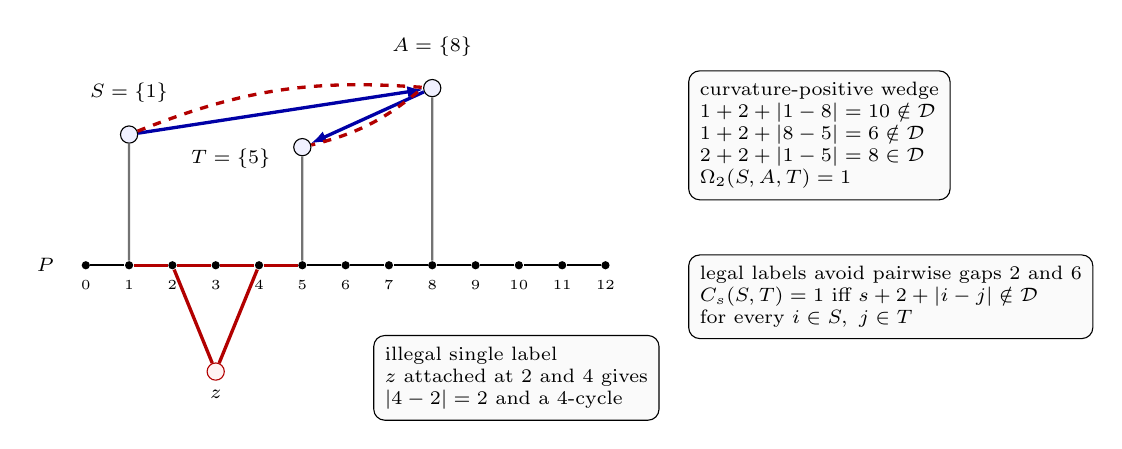
\begin{tikzpicture}[
pvert/.style={circle,fill=black,inner sep=1.05pt},
outside/.style={circle,draw,fill=blue!6,inner sep=2.2pt},
illegal/.style={circle,draw=red!70!black,fill=red!5,inner sep=2.2pt},
safe/.style={-{Latex[length=2mm]},very thick,blue!65!black},
unsafe/.style={very thick,red!70!black},
attach/.style={thick,black!55},
box/.style={rectangle,rounded corners,draw,align=left,inner sep=4pt,fill=black!2},
every node/.style={font=\scriptsize}
]
\foreach \i in {0,...,12} {
  \node[pvert] (v\i) at (-4.40+0.55*\i,0) {};
  \node[font=\tiny,below=2pt] at (-4.40+0.55*\i,0) {$\i$};
}
\draw[thick] (v0)--(v1)--(v2)--(v3)--(v4)--(v5)--(v6)--(v7)--(v8)--(v9)--(v10)--(v11)--(v12);
\node[anchor=east] at (-4.68,0) {$P$};

% Curvature-positive wedge.
\node[outside] (S) at (-3.85,1.66) {};
\node[anchor=south] at (-3.85,1.94) {$S=\{1\}$};
\node[outside] (A) at (0.00,2.25) {};
\node[anchor=south] at (0.00,2.53) {$A=\{8\}$};
\node[outside] (T) at (-1.65,1.50) {};
\node[anchor=east] at (-1.93,1.35) {$T=\{5\}$};
\draw[attach] (S)--(v1);
\draw[attach] (A)--(v8);
\draw[attach] (T)--(v5);
\draw[safe] (S)--(A);
\draw[safe] (A)--(T);
\draw[unsafe] (v1)--(v2)--(v3)--(v4)--(v5);
\draw[unsafe,dashed] (S) to[bend left=13] (A) to[bend left=13] (T);
\node[box,anchor=west] at (3.25,1.65)
{curvature-positive wedge\\
\(1+2+|1-8|=10\notin\Pow\)\\
\(1+2+|8-5|=6\notin\Pow\)\\
\(2+2+|1-5|=8\in\Pow\)\\
\(\Omega_2(S,A,T)=1\)};

% Illegal label inset on the same path.
\node[illegal,label=below:$z$] (z) at (-2.75,-1.35) {};
\draw[unsafe] (z)--(v2);
\draw[unsafe] (z)--(v4);
\draw[unsafe] (v2)--(v3)--(v4);
\node[box,anchor=west] at (-0.75,-1.43)
{illegal single label\\
\(z\) attached at \(2\) and \(4\) gives\\
\(|4-2|=2\) and a \(4\)-cycle};

\node[box,anchor=west] at (3.25,-0.40)
{legal labels avoid pairwise gaps \(2\) and \(6\)\\
\(C_s(S,T)=1\) iff \(s+2+|i-j|\notin\Pow\)\\
for every \(i\in S,\ j\in T\)};
\end{tikzpicture}%
}
\caption[Visual definition of \(P_{13}\) labels and two-step curvature]{Visual definition of the \(P_{13}\) label algebra and the two-step curvature tensor.  The black horizontal path is the induced \(P_{13}\), with indices \(0,\ldots,12\) displayed below its vertices.  An outside vertex has label equal to the set of path indices to which it is adjacent.  The lower red vertex \(z\) illustrates an illegal label: attachments at indices \(2\) and \(4\) close a \(4\)-cycle through the subpath \(v_2v_3v_4\), so legal labels must avoid pairwise gaps \(2\) and \(6\).  The upper vertices carry the singleton labels \(S=\{1\}\), \(A=\{8\}\), and \(T=\{5\}\).  The blue outside edges show the two individually safe length-\(1\) relations \(C_1(S,A)=1\) and \(C_1(A,T)=1\).  The dashed red two-step outside path from \(S\) to \(T\), together with the red path segment \(v_1\cdots v_5\) and the two attachment edges, has length \(2+2+|1-5|=8\); hence \(C_2(S,T)=0\).  Thus \(\Omega_2(S,A,T)=1\): two locally safe outside steps compose into an unsafe dyadic test.}
\label{fig:p13-curvature-label-gadget}
\end{figure}

\begin{lemma}[Curvature enumeration]\label[lemma]{lem:curv-enum}
For the $399$ legal labels,
\[
|\{(S,A,T):C_1(S,A)=C_1(A,T)=1\}|=543958,
\]
and
\[
|\{(S,A,T):\Omega_2(S,A,T)=1\}|=432672.
\]
Hence the number of curvature-flat locally safe wedges is
\[
111286.
\]
Therefore the flatness entropy cost of one independent two-step curvature test is
\[
\boxed{
 c_\Omega=\log_2\frac{543958}{111286}=2.28922315244\ldots.
 }
\]
\end{lemma}

\begin{proof}
The proof is the same direct finite enumeration as in \cref{lem:labels}, now applied to ordered triples of legal labels.  A locally safe wedge is a triple $(S,A,T)$ with $C_1(S,A)=C_1(A,T)=1$.  It is curvature-positive when $C_2(S,T)=0$.  The code in \cref{app:curv-code} performs precisely these tests and returns the displayed integer counts.  The entropy value is then the elementary calculation
\[
\log_2\frac{543958}{111286}=2.28922315244071\ldots .
\]
\end{proof}

A finite-scale multi-relation curvature package through length $14$ yields the constant
\[
\boxed{c_{13}=118.108581006\ldots}
\]
bits per independent $P_{13}$-window package per dyadic scale.  This value is the sum of the $91$ finite curvature barriers indexed by ordered pairs of outside path lengths $a,b\ge1$ with $a+b\le14$.  The number of such pairs is
\[
\bigl|\{(a,b):a,b\ge1,\ a+b\le14\}\bigr|=\sum_{s=2}^{14}(s-1)=\sum_{k=1}^{13}k=91,
\]
since for each total $s=a+b\in\{2,\ldots,14\}$ there are exactly $s-1$ admissible pairs $(a,s-a)$ with $1\le a\le s-1$; the individual barriers are computed in \cref{app:curv-code}.

\paragraph{Framework branch table.}
The curvature-algebra section is a finite computation interface: every
quantity it exports is either an integer count or a named entropy rate
verified in \cref{app:curv-code}.
\begin{longtable}{L{0.13\textwidth} L{0.19\textwidth} L{0.14\textwidth} L{0.14\textwidth} L{0.17\textwidth} L{0.17\textwidth}}
\FrameworkBranchTableHeader
Illegal label
&
An outside vertex attaches at path-index distance \(2\) or \(6\).
&
The attachment label \(S\).
&
The target predicate.
&
The induced path segment plus two attachment edges is a \(4\)- or \(8\)-cycle.
&
Excluded by the counterexample condition.
\\
\addlinespace
Legal label enumeration
&
All nonempty labels avoiding gaps \(2\) and \(6\).
&
The finite set \(\labels\).
&
Direct enumeration.
&
The code tests every subset of \(\{0,\ldots,12\}\).
&
\cref{lem:labels}.
\\
\addlinespace
Two-step curvature test
&
\(C_1(S,A)=C_1(A,T)=1\) but \(C_2(S,T)=0\).
&
The triple \((S,A,T)\).
&
The finite curvature tensor.
&
The same predicates define both the proof and the code check.
&
\cref{lem:curv-enum}.
\\
\addlinespace
Multi-scale package constant
&
Ordered path-length pairs \(a,b\ge1\), \(a+b\le14\).
&
The \(91\) barrier rates.
&
The computational certificate.
&
The exported value is the displayed sum \(c_{13}=118.108581006\ldots\).
&
Consumed by \cref{lem:p13-window-package}.
\\
\bottomrule
\end{longtable}

\section{Entropy bound on independent \texorpdfstring{$P_{13}$}{P13} windows}\label{sec:entropy-bound}

This section carries out the normalized entropy accounting under
\cref{def:near-cubic-spine} in the high-entropy
(window) branch of the routing in \cref{prop:two-budget}, in which the
remainder contributes its full per-vertex skeleton entropy.  Let $R$ be the
complement of a maximal disjoint induced-$P_{13}$ packing.  The next lemma is
the window package consumed by the density bound.

\begin{lemma}[Independent multi-scale \(P_{13}\)-window package]\label[lemma]{lem:p13-window-package}
Assume the sparse surplus exits have been discharged and the near-cubic spine
estimate of \cref{def:near-cubic-spine} has been supplied.  Let
\(\mathcal P\) be a maximal vertex-disjoint induced-\(P_{13}\) packing in \(G\).
Then the canonical multi-scale package attached to \(\mathcal P\) contains a
family \(\mathcal I_{\rm win}\) of independently target-testable coordinates
with
\[
|\mathcal I_{\rm win}|
\ge
\bigl(c_{13}-o(1)\bigr)|\mathcal P|\log_2 n,
\qquad
c_{13}=118.108581006\ldots .
\]
The package is the disjoint union of the packages attached to the distinct
packed windows.  Hence no coordinate is counted for two windows.  Moreover, in
any entropy comparison in which a baseline spine coordinate family is already
present, \(\mathcal I_{\rm win}\) is adjoined to that family as independent
target coordinates before \cref{lem:independent-target-entropy} is applied.
\end{lemma}

\begin{proof}
Fix one packed induced \(P_{13}\), with path vertices \(v_0,\ldots,v_{12}\).
For an outside path of length \(s\), the finite label relation \(C_s(S,T)\)
records exactly which ordered pairs of legal \(P_{13}\)-labels can be joined
without creating a dyadic cycle through the window.  For every ordered pair
\((a,b)\) with \(a,b\ge1\) and \(a+b\le14\), let \(W_{a,b}\) be the number of
locally safe triples \((S,A,T)\) with
\[
C_a(S,A)=C_b(A,T)=1,
\]
and let \(F_{a,b}\) be the number of those triples that remain safe after the
composed outside path is tested, i.e. with \(C_{a+b}(S,T)=1\).  The
\((a,b)\)-barrier therefore has flatness cost
\[
\gamma_{a,b}=\log_2(W_{a,b}/F_{a,b}).
\]
The direct finite computation in \cref{app:curv-code} evaluates these numbers
for all
\[
\{(a,b):a,b\ge1,\ a+b\le14\},
\]
and gives
\[
\sum_{a,b}\gamma_{a,b}=118.10858100609198\ldots=c_{13}.
\]

The multi-scale package uses \(\lfloor\log_2 n\rfloor-O(1)\) separated dyadic
scales for these finite barriers.  The \(O(1)\) loss absorbs endpoint
collisions with the finitely many reserved boundary and tie-breaking choices
inside the canonical packing.  At each remaining scale, the target tester is
the corresponding edge-rooted Mersenne completion through the window.  The
relations \(C_a,C_b,C_{a+b}\) were defined precisely so that changing the
barrier state changes that tester and leaves the other displayed coordinates
fixed.  Thus, for one window, the package supplies
\[
\left(\sum_{a,b}\gamma_{a,b}-o(1)\right)\log_2 n
=
\bigl(c_{13}-o(1)\bigr)\log_2 n
\]
independently target-testable coordinates.

Distinct packed windows are vertex-disjoint, and the canonical assignment of a
coordinate records the unique packed window through which its tester is routed.
The product of the target-complete states on the distinct windows is therefore
again target-complete; equivalently, the tester for one window does not change
the label state assigned to another packed window.  The window packages are
therefore independent across \(\mathcal P\), giving the displayed lower bound.
The same product argument applies when a baseline spine family has already been
declared: the baseline coordinates and the window coordinates are combined into
one independently target-testable family, and only then is the labelled
skeleton bound of \cref{lem:independent-target-entropy,lem:skeleton-dominates}
applied.  Hence the window coordinates are not counted twice.
\end{proof}

\begin{definition}[Hot/cold window ledger]\label[definition]{def:cold-window-ledger}
Set
\[
c_{\rm hot}:=118.10858100609198\ldots,
\qquad
\theta_{\rm win}:=\frac{3}{2c_{\rm hot}}
=0.012700177982179218\ldots .
\]
For a packing density \(\theta=p_{13}/n\), set
\[
\tau(\theta):=\frac{15\theta}{1-13\theta}.
\]
Then
\[
\tau(\theta)<\frac14
\quad\Longleftrightarrow\quad
\theta<\frac1{73}=0.0136986301369863\ldots,
\]
and
\[
\tau(\theta)<\frac3{13}
\quad\Longleftrightarrow\quad
\theta<\frac1{78}=0.0128205128205128\ldots .
\]
The value \(1/78\) is the route-8 private-carrier threshold, and \(1/73\) is
the negative-net-charge threshold.

Fix a maximal vertex-disjoint induced-\(P_{13}\) packing \(\mathcal P\) and the
canonical entropy comparison used on the branch under discussion.  A packed
window is \emph{hot} when that comparison contains, for this window, the full
canonical package of independently target-testable coordinates with rate
\[
(c_{\rm hot}-o(1))\log_2 n .
\]
Equivalently, hotness is witnessed by the injective list of declared window
coordinates supplied by \cref{lem:p13-window-package} for that window and
retained in the current comparison.  A packed window not carrying such a live
package in the current comparison is \emph{cold}.  We write
\[
\mathcal P=\mathcal P_{\rm hot}\sqcup\mathcal P_{\rm cold},
\qquad
C:=|\mathcal P_{\rm cold}|.
\]
\end{definition}

\begin{definition}[Surviving cold branch]\label[definition]{def:surviving-cold-branch}
The \emph{surviving cold branch} is the branch on which:
\begin{enumerate}[label=(\roman*), leftmargin=2.2em]
\item no target cycle has been found;
\item no sparse surplus exit, target-defective quotient, target-complete
compression, or delocalization exit is active;
\item no unpaid exit-\textup{(4)} peel remains;
\item no Type B bridge or handoff residual remains outside its ledger;
\item no Type A route-8 residual remains outside
\cref{thm:large-budget-route8-only}; and
\item the sparse surplus branch has already supplied the spine estimate in the
form \(m=\frac32 n+o(n)\) and \(\sigma(G)=2m-3n=o(n)\).
\end{enumerate}
On this branch, \(|V_{\ge4}(G)|\le\sigma(G)=o(n)\).  Hence all but \(o(n)\)
packed \(P_{13}\)-windows are ambient-cubic.
\end{definition}

\begin{lemma}[Hot failure forces cold mass]\label[lemma]{lem:hot-failure-cold-mass}
Assume \cref{def:surviving-cold-branch}.  If the live-hot entropy comparison
does not close, then
\[
C\ge(\theta-\theta_{\rm win})n-o(n).
\]
In particular, at the route-8 threshold \(\theta=1/78\),
\[
C\ge0.000120334838333602\,n-o(n),
\]
and at the negative-net-charge threshold \(\theta=1/73\),
\[
C\ge0.000998452154807083\,n-o(n).
\]
\end{lemma}

\begin{proof}
The hot windows contribute at least
\[
\bigl(c_{\rm hot}-o(1)\bigr)|\mathcal P_{\rm hot}|\log_2 n
\]
independently target-testable coordinates.  If these coordinates alone exceed
the near-cubic skeleton budget \(\frac32 n\log_2 n+o(n\log n)\), then
\cref{lem:independent-target-entropy,lem:skeleton-dominates} close the branch.
Therefore, on a branch where the hot comparison has not closed,
\[
c_{\rm hot}|\mathcal P_{\rm hot}|\log_2 n
\le
\frac32 n\log_2 n+o(n\log n).
\]
Dividing by \(c_{\rm hot}\log_2 n\) gives
\[
|\mathcal P_{\rm hot}|
\le
\frac{3}{2c_{\rm hot}}n+o(n)
=\theta_{\rm win}n+o(n).
\]
Since \(p_{13}=|\mathcal P|=\theta n\),
\[
C=|\mathcal P|-|\mathcal P_{\rm hot}|
\ge(\theta-\theta_{\rm win})n-o(n).
\]
The two displayed numerical lower bounds are obtained by substituting
\(\theta=1/78\) and \(\theta=1/73\).
\end{proof}

\begin{definition}[Cold skeleton and branch excess]\label[definition]{def:cold-skeleton-excess}
Let
\[
\mathcal P_{\rm cold}^{\rm cub}
:=\{P\in\mathcal P_{\rm cold}: V(P)\cap V_{\ge4}(G)=\varnothing\}.
\]
By \cref{def:surviving-cold-branch},
\[
|\mathcal P_{\rm cold}\setminus\mathcal P_{\rm cold}^{\rm cub}|=o(n).
\]
For each \(P\in\mathcal P_{\rm cold}^{\rm cub}\), contract the path \(P\) to
one skeleton vertex \(p\) and keep one incident half-edge for every edge of
\(G\) leaving \(P\).  The resulting incidence object is the
\emph{ambient-cubic cold skeleton} \(\mathfrak S_{\rm cold}\).  If \(s(P)\) is
the number of external stubs of \(P\), define the branch-excess contribution of
\(P\) by
\[
b(P):=\max\{0,s(P)-2\},
\]
and set
\[
b(\mathfrak S_{\rm cold})
:=\sum_{P\in\mathcal P_{\rm cold}^{\rm cub}} b(P).
\]

The branch-excess units are selected concretely as follows.  The global
lexicographic order on vertices and edges induces an order on the external
stubs of every ambient-cubic cold window.  The first two stubs of \(P\) are
called the \emph{transit stubs}; the remaining \(s(P)-2\) stubs, when
\(s(P)>2\), are the \emph{selected branch-excess half-edges} of \(P\).  Let
\[
\mathcal E_{\rm br}(P)
\]
be this selected set and let
\[
\mathcal E_{\rm br}:=\bigcup_P\mathcal E_{\rm br}(P).
\]
Thus
\[
|\mathcal E_{\rm br}|=b(\mathfrak S_{\rm cold}).
\]
All later cold-branch counts are counts of these selected half-edges.  Hence a
stub can be charged at most once at its cold-window endpoint.
\end{definition}

\begin{lemma}[Cold window stub excess]\label[lemma]{lem:cold-window-stub-excess}
On \cref{def:surviving-cold-branch},
\[
b(\mathfrak S_{\rm cold})\ge13C-o(n).
\]
\end{lemma}

\begin{proof}
Let \(P\) be an ambient-cubic induced \(P_{13}\) with vertices
\(v_0,\ldots,v_{12}\).  The internal path edges contribute
\[
2\cdot12=24
\]
to the sum of degrees inside \(P\), while the ambient cubic degrees contribute
\[
13\cdot3=39.
\]
Thus \(P\) has exactly \(39-24=15\) external stubs.  In the skeleton, a
degree-two corridor through \(p\) can absorb at most two of these stubs without
branching.  Hence \(b(P)=15-2=13\) for every ambient-cubic cold window.  By
\cref{def:surviving-cold-branch}, only \(o(n)\) cold windows are not
ambient-cubic.  Summing over the remaining windows gives the claim.
\end{proof}

\begin{lemma}[Short self-return filter]\label[lemma]{lem:cold-short-self-return-filter}
Let a cold-window outside self-return have outside length \(\ell\).  Smearing
over the window offsets \(\{0,1,\ldots,12\}\) tests the whole interval
\([\ell,\ell+12]\).  For \(1\le\ell\le39\), the interval avoids
\(\{4,8,16,32\}\) only for
\[
\ell\in\{17,18,19,33,34,35,36,37,38,39\}.
\]
For \(1\le\ell\le32\), the only surviving lengths are
\[
\ell\in\{17,18,19\}.
\]
All other short self-returns realize a dyadic cycle.
\end{lemma}

\begin{proof}
The interval \([\ell,\ell+12]\) contains \(4\) exactly when
\(1\le\ell\le4\), contains \(8\) exactly when \(1\le\ell\le8\), contains
\(16\) exactly when \(4\le\ell\le16\), and contains \(32\) exactly when
\(20\le\ell\le32\).  Their union inside \(\{1,\ldots,39\}\) is
\[
\{1,\ldots,16\}\cup\{20,\ldots,32\}.
\]
The complement is precisely the displayed set.  Intersecting this complement
with \(\{1,\ldots,32\}\) gives \(\{17,18,19\}\).  If the interval contains one
of \(4,8,16,32\), the corresponding offset closes a cycle of that length
through the window, contradicting the counterexample condition.
\end{proof}

\begin{definition}[Cold bounded germ]\label[definition]{def:cold-bounded-germ}
A \emph{cold bounded germ} is a finite boundaried support with two boundary
interfaces \(x,y\) and two same-interface \(x\)-\(y\) representatives
\(Q[x,y]\) and \(E\).  In a terminal corridor these representatives are the
two bounded completion strands between the same interfaces; in a repeated-state
corridor one representative is the actual corridor segment and the other is
the canonical representative determined by the repeated cold corridor state.
The germ also carries the inherited boundary degree profile,
\(P_{13}\)-window labels, and target-response profile.  Its increment is
\[
\delta:=|E|-|Q[x,y]|.
\]
It is \emph{length-changing} if \(\delta\ne0\), and \emph{equal-length} if
\(\delta=0\).  The word bounded means that the number of internal vertices and
all boundary data are bounded by the fixed finite cut-state constant used by
the local target algebra; consequently there are only finitely many germ
types.
\end{definition}

\begin{definition}[Cold corridor states and first failures]\label[definition]{def:cold-corridor-first-failure}
Let \(X_{\rm cold}\) be the union of the ambient-cubic cold windows, with their
internal path edges retained.  Delete the interiors of these windows and look
at a connected component \(K\) of the remaining outside graph.  The
\emph{boundary stubs} of \(K\) are the edges from \(K\) to ambient-cubic cold
windows.  By \cref{lem:bridgeless}, no such component has only one boundary
stub, since that unique boundary edge would be a bridge of \(G\).

Order the boundary stubs of \(K\) lexicographically as
\[
h_1,\ldots,h_m\qquad(m\ge2)
\]
and give them the cyclic successor relation \(h_i\mapsto h_{i+1}\), with
\(h_{m+1}=h_1\).  If \(h_i=\epsilon\in\mathcal E_{\rm br}(P)\) is a selected
branch-excess half-edge, choose inside \(K\) the lexicographically first simple
path joining the outside endpoint of \(h_i\) to the outside endpoint of
\(h_{i+1}\).  Together with the two boundary stubs \(h_i,h_{i+1}\), this path
is the \emph{cold return corridor} of \(\epsilon\).  Thus each selected
branch-excess half-edge has exactly one corridor, and each boundary stub is the
successor of at most one selected half-edge.

For an initial segment \(J\) of this corridor, let \(T(J)\) be its two active
boundary interfaces.  Its \emph{cold corridor state} is the finite
two-boundary cut-state obtained from
\(\rho_{T(J)}^{\rm ex}(J)\) by retaining exactly the boundary-degree profile,
the two active boundary half-edges, the cold-window offsets met at the two
interfaces, and the declared local coordinates of
\cref{def:declared-coordinate-signature} whose support is contained in the
bounded active interface.  It is not the full labelled prefix.  If two prefixes
have the same finite cut-state but differ in exact target response against
some compatible context, that discrepancy is recorded as a first failure of
type \textup{(F2)} below.  Thus, after excluding (F2), equality of cold
corridor states is equality for every target-response coordinate used by the
local replacement.  Since the boundary has size two and the retained window
and local-coordinate labels are finite, the set of possible cold corridor
states is bounded by a constant \(Q_{\rm cold}\) depending only on the fixed
declared signature.
Set
\[
M_{\rm cold}:=Q_{\rm cold}+30,\qquad
B_{\rm cold}:=15\bigl(1+3(2^{M_{\rm cold}+2}-1)\bigr),\qquad
D_{\rm cold}:=M_{\rm cold}B_{\rm cold}+1.
\]
The additive \(30\) only covers the two \(P_{13}\)-window interfaces and the
two boundary stubs.  Thus \(M_{\rm cold}\) is a uniform upper bound for the
number of vertices in a first-failure cold exchange, and \(B_{\rm cold}\) is a
uniform upper bound for the number of selected cold half-edges whose
first-failure support can contain a fixed subcubic vertex.

The \emph{first failure} of \(\epsilon\) is the first initial segment, in the
lexicographic order along the corridor, at which one of the following happens:
\begin{enumerate}[label=(F\arabic*), leftmargin=2.4em]
\item a compatible completion through a cold-window offset realizes a
power-of-two cycle;
\item two prefixes with the same displayed boundary data have different
target response against some compatible outside context;
\item two prefixes have the same exact target response against every outside
context and one gives a strictly smaller proper representative;
\item the corridor first enters a declared Type B handoff envelope or the
route-8 carrier support already recorded in the branch state;
\item no earlier alternative occurs and either the corridor reaches its
successor boundary stub before \(Q_{\rm cold}+1\) states have been read, or a
cold corridor state repeats.
\end{enumerate}
In case (F5), the bounded support is the whole terminal corridor in the first
subcase, and the support between the two equal states in the second subcase.
With its two boundary interfaces, this bounded support is the
\emph{first-failure cold exchange} of \(\epsilon\).
\end{definition}

\begin{lemma}[Cold corridor first-failure routing]\label[lemma]{lem:cold-corridor-first-failure}
Assume \cref{def:surviving-cold-branch}.  For every
\(\epsilon\in\mathcal E_{\rm br}\), the cold return corridor of \(\epsilon\)
has a first failure.  The first failure is routed as follows:
\begin{enumerate}[label=(\roman*), leftmargin=2.2em]
\item case \textup{(F1)} is a dyadic cycle in \(G\);
\item case \textup{(F2)} is a target-defective quotient, hence belongs to the
sparse exit or to the exit-\textup{(4)} ledger;
\item case \textup{(F3)} is a target-complete compression of a proper support;
\item case \textup{(F4)} is an already named Type B or route-8 handoff;
\item case \textup{(F5)} is a cold bounded germ in the sense of
\cref{def:cold-bounded-germ}.
\end{enumerate}
Consequently, on the surviving cold branch, every selected branch-excess
half-edge that is not in the already discarded \(o(n)\) handoff or surplus
ledgers supplies a canonical cold bounded-germ incidence.
\end{lemma}

\begin{proof}
The return corridor exists by \cref{lem:bridgeless}.  Follow its initial
segments until one of the alternatives in
\cref{def:cold-corridor-first-failure} occurs.  If the successor boundary stub
is reached before \(Q_{\rm cold}+1\) states have been read, then the whole
corridor, together with the two boundary stubs and the two \(P_{13}\)-window
interfaces, has at most \(M_{\rm cold}=Q_{\rm cold}+30\) vertices and gives the
terminal subcase of (F5).  Otherwise, before the successor is reached,
\(Q_{\rm cold}+1\) states are read; two states are equal by the definition of
\(Q_{\rm cold}\), and the first such equality gives the repeat subcase of
(F5).  Hence a first failure always exists.

If the first failure is (F1), the displayed completion is literally a cycle of
power-of-two length in \(G\), impossible in a counterexample.  If it is (F2),
the actual quotient is valid only for the current outside context and fails
for another compatible context.  By \cref{lem:context-universality}, this is
not target-complete, so it is a target-defective quotient.  In the global
branch ledger such defects are exactly the sparse exits; in the Type A
location they are the exit-\textup{(4)} peels, and both are excluded in
\cref{def:surviving-cold-branch}.

In (F3), context-universality holds and the displayed representative is
strictly smaller while preserving the boundary-degree profile and the exact
target response.  Thus it satisfies
\cref{def:proper-quotient-representative} and is forbidden by
\cref{lem:replacement,cor:uncompressible}.  In (F4), the corridor has reached
precisely one of the declared interfaces of
\cref{def:decorated-fan-envelope} or the route-8 carrier support, so the
charge is transferred to the already existing Type B or route-8 ledger.

It remains to consider (F5).  In the terminal subcase, the whole corridor has
bounded size and two boundary interfaces.  In the repeat subcase, the two
repeated states have the same two boundary interfaces, the same inherited
boundary-degree profile, the same window labels, and the same exact
target-response coordinates; the support between them is bounded by
\(Q_{\rm cold}\).  In both subcases the support carries two same-interface
representatives: the actual corridor representative and the terminal or
repeated-state exchange representative with the same retained cut-state.  Thus
it is a cold bounded germ in the sense of \cref{def:cold-bounded-germ}.  All
cases except (F5) are excluded on the surviving branch, up to the \(o(n)\)
windows and corridors already charged to the non-ambient-cubic, handoff, or
surplus ledgers.  Hence every remaining selected branch-excess half-edge
supplies a canonical bounded-germ incidence.
\end{proof}

\begin{lemma}[Cold branch-excess extracts bounded germs]\label[lemma]{lem:cold-germ-extraction}
Assume \cref{def:surviving-cold-branch}.  If the cold skeleton has branch
excess \(b=b(\mathfrak S_{\rm cold})\), then it contains a family of pairwise
vertex-disjoint candidate cold bounded germs of size
\[
N_{\rm germ}\ge\frac{b}{D_{\rm cold}}-o(n).
\]
In particular, after hot failure,
\[
N_{\rm germ}
\ge
\frac{13C}{D_{\rm cold}}-o(n)
\ge
\frac{13(\theta-\theta_{\rm win})}{D_{\rm cold}}\,n-o(n).
\]
\end{lemma}

\begin{proof}
By \cref{def:cold-skeleton-excess}, there are exactly
\(b=|\mathcal E_{\rm br}|\) selected branch-excess half-edges, and each is
selected once.  By \cref{lem:cold-corridor-first-failure}, after deleting the
already routed \(o(n)\) surplus, non-ambient-cubic, Type B, and route-8
handoff incidences, each remaining selected half-edge supplies one canonical
first-failure cold bounded germ.  Let \(\mathcal G_{\rm cand}\) be this
candidate family.  Then
\[
|\mathcal G_{\rm cand}|\ge b-o(n).
\]

It remains only to extract a vertex-disjoint subfamily without double-counting
overlapping local supports.  Each member of \(\mathcal G_{\rm cand}\) has at
most \(M_{\rm cold}\) vertices by
\cref{def:cold-corridor-first-failure}.  If a candidate support contains a
vertex of degree at least \(4\), then the corresponding corridor first enters
the high-degree handoff ledger and was already removed; hence every remaining
candidate lies in the subcubic part of the surviving branch.  In a subcubic
graph the ball of radius \(M_{\rm cold}+2\) around a vertex has at most
\[
1+3(2^{M_{\rm cold}+2}-1)
\]
vertices, and every ambient-cubic cold window contributes at most \(15\)
external stubs.  Therefore a fixed vertex belongs to the support of at most
\[
B_{\rm cold}=15\bigl(1+3(2^{M_{\rm cold}+2}-1)\bigr)
\]
candidate germs.  A fixed candidate support has at most \(M_{\rm cold}\)
vertices, so it meets at most \(M_{\rm cold}B_{\rm cold}\) other candidate
supports.  The intersection graph of \(\mathcal G_{\rm cand}\) thus has
maximum degree at most \(M_{\rm cold}B_{\rm cold}\).

A greedy maximal independent set in a graph of maximum degree \(\Delta\) has
size at least the number of vertices divided by \(\Delta+1\).  With
\(\Delta=M_{\rm cold}B_{\rm cold}\), this gives a vertex-disjoint candidate
germ family of size
\[
N_{\rm germ}\ge
\frac{|\mathcal G_{\rm cand}|}{M_{\rm cold}B_{\rm cold}+1}
\ge
\frac{b}{D_{\rm cold}}-o(n).
\]
The remaining inequalities use
\cref{lem:cold-window-stub-excess,lem:hot-failure-cold-mass}.
\end{proof}

\begin{lemma}[Bounded germ trichotomy]\label[lemma]{lem:cold-bounded-germ-trichotomy}
No length-changing cold bounded germ survives on
\cref{def:surviving-cold-branch}.  More explicitly, every such germ falls into
one of the following three cases:
\begin{enumerate}[label=\textup{G\arabic*.}, leftmargin=3.2em]
\item \emph{Hit-realized.}  Some compatible live completion and window offset
close a dyadic cycle.  This contradicts the counterexample condition.
\item \emph{Hit-distinguished.}  Some compatible outside context distinguishes
the two representatives by dyadic truth value without already realizing the
cycle in the current graph.  The induced quotient is target-defective, so it is
routed to the sparse exit or exit-\textup{(4)} ledger.
\item \emph{Silent.}  No compatible outside context and no relevant scale
distinguishes the two representatives.  Then replacing the longer
representative by the shorter one preserves the boundary degree profile and the
target response against every context, creates no dyadic cycle, and strictly
decreases the support.  This is a nontrivial target-complete compression of a
proper support.
\end{enumerate}
Each case is impossible on the surviving cold branch.
\end{lemma}

\begin{proof}
The cases are exhaustive by whether a compatible completion realizes a dyadic
hit, distinguishes dyadic truth without realization in \(G\), or never
distinguishes the two representatives.

In G1, the completed representative plus the relevant window segment is a cycle
whose length is a power of two.  This contradicts the definition of a
counterexample.

In G2, the two local responses agree in the actual quotient but disagree in a
compatible context.  By \cref{lem:context-universality}, such an identification
is not target-complete; equivalently it is a target-defective quotient.  This
is one of the named surplus exits or, inside Type A, an exit-\textup{(4)} peel.
Both are excluded by \cref{def:surviving-cold-branch}.

In G3, all compatible contexts give the same target response for the two
representatives.  Because \(\delta\ne0\), one representative is strictly
longer.  Replacing the longer representative by the shorter one keeps the same
boundary vertices, the same boundary degree profile, and the same target
response against every context.  It cannot create a dyadic cycle, since any
such cycle would distinguish the two responses.  Thus the replacement is a
smaller target-complete
representative of a proper support, forbidden by
\cref{lem:replacement,cor:uncompressible}.  Hence no length-changing bounded
germ survives.
\end{proof}

\begin{definition}[Finite same-interface cold table]\label[definition]{def:cold-same-interface-table}
The \emph{same-interface cold table} is the finite table whose rows are
equal-length cold bounded germs and the short self-return exceptions of
\cref{lem:cold-short-self-return-filter}, recorded with:
\begin{enumerate}[label=(T\arabic*), leftmargin=2.4em]
\item the two boundary vertices and their boundary-degree profile;
\item the two terminal cold-window stubs and their offsets in
\(\{0,\ldots,12\}\);
\item the exact response profile generated by
\cref{def:declared-coordinate-signature};
\item the target truth value of every compatible completion represented by
that exact profile.
\end{enumerate}
The table is finite because the support size, boundary size, window labels,
and declared coordinate labels are bounded by
\cref{def:cold-corridor-first-failure}.  A row is \emph{realizing} if some
compatible completion gives a power-of-two cycle, \emph{distinguishing} if two
same-interface representatives have different target truth value in some
compatible context, and \emph{neutral} otherwise.
\end{definition}

\begin{lemma}[Same-interface cold table closure]\label[lemma]{lem:cold-same-interface-table}
Every row of the same-interface cold table is routed to one of the already
closed outcomes: a dyadic cycle, a target-defective quotient, an existing
Type B or route-8 handoff, or a target-complete proper-support compression.
In particular, an equal-length cold bounded germ and a short exceptional
self-return cannot be a terminal cold residual.
\end{lemma}

\begin{proof}
Let \(R\) be a row of the table.  If \(R\) is realizing, the corresponding
completion is a power-of-two cycle in \(G\), which contradicts the
counterexample condition.  If \(R\) first meets a declared Type B or route-8
interface, then by the definition of the surviving cold branch the charge is
transferred to that already closed ledger.

Assume \(R\) is not realizing and does not enter a handoff interface.  If
there is a compatible context distinguishing the two same-interface
representatives, then \cref{lem:context-universality} says that their
identification is not target-complete.  This is a target-defective quotient,
hence a sparse exit or an exit-\textup{(4)} peel, both excluded by
\cref{def:surviving-cold-branch}.

It remains to handle a neutral row.  Neutrality means that the two
representatives have the same boundary-degree profile and the same target
response against every compatible context.  The row is a first-failure row:
otherwise it would not have entered the cold table.  Therefore the quotient
identifying the two same-interface representatives removes at least one
declared branch-excess coordinate while preserving every coordinate needed by
the target response.  By \cref{def:admissible-rank-quotient}, such a
proper-support target-complete quotient is admissible only when it has a
strictly smaller proper representative in the sense of
\cref{def:proper-quotient-representative}.  That representative satisfies the
hypotheses of \cref{lem:replacement}, and is forbidden by
\cref{cor:uncompressible}.  Hence no neutral row survives either.
\end{proof}

\begin{lemma}[Increment arithmetic for cold germs]\label[lemma]{lem:cold-increment-arithmetic}
Let a homogeneous cold germ have increment \(\delta\), oriented so
\(\delta\ge0\).  The following cases exhaust the finite arithmetic:
\begin{enumerate}[label=(\alph*), leftmargin=2.2em]
\item If \(1\le\delta\le12\), then the achievable length blocks
\[
[L+j\delta,L+j\delta+12]\qquad(0\le j\le N)
\]
overlap.  If their union spans a dyadic scale, the branch is G1; otherwise the
whole family lies in one bounded dyadic gap and is a bounded germ type handled
by \cref{lem:cold-bounded-germ-trichotomy}.
\item If \(\delta\ge13\) and the doubling orbit modulo \(\delta\) hits one of
the thirteen smear residues \(L,L+1,\ldots,L+12\), the branch is G1.
\item If \(\delta\ge13\) and the doubling orbit avoids all thirteen smear
residues, the odd part of \(\delta\) gives a periodic carrier.  A
target-visible carrier is G2, and a target-invisible carrier is G3.
\item If \(\delta=0\), the equal-length switch belongs to the finite
same-interface cold table; each table row is closed by
\cref{lem:cold-same-interface-table}.
\end{enumerate}
For odd \(\delta\), the sufficient hit criterion
\[
\operatorname{ord}_{\delta}(2)>\delta-13
\]
forces case (b).  For even \(\delta=2^a u\), the same criterion applies to the
odd part \(u\) after the bounded transient \(k<a\).
\end{lemma}

\begin{proof}
For (a), consecutive blocks overlap because the next block begins at
\(L+(j+1)\delta\le L+j\delta+12\).  Hence their union is an interval.  An
interval containing a power of two gives G1; if it contains none, all
corresponding completions live inside one bounded gap between consecutive
powers of two, so only finitely many target-response types occur and
\cref{lem:cold-bounded-germ-trichotomy} applies.

For (b), a congruence \(2^k\equiv L+r\pmod\delta\) with \(0\le r\le12\) means
that, after adding the appropriate number of homogeneous copies, one attainable
length is \(2^k\).  This is exactly a hit-realized germ.

For (c), avoidance of all smear residues means the orbit of powers of two is
confined to the complement of the thirteen target residues modulo the odd
part of \(\delta\).  The residue class is then a periodic carrier.  If some
compatible context sees the carrier, the two representative responses are
target-distinguished and G2 applies.  If no compatible context sees it, the
carrier is target-equivalent and G3 applies.

For (d), equal-length switches cannot be charged as length-changing
increments.  They are finite because the germ support and boundary data are
bounded, and \cref{lem:cold-same-interface-table} closes every row of the
finite same-interface table.

If \(\delta\) is odd and \(\operatorname{ord}_{\delta}(2)>\delta-13\), the
doubling orbit has more residues than the complement of the thirteen smear
residues.  Therefore it must hit a smear residue, giving (b).  If
\(\delta=2^a u\), the initial powers with \(k<a\) form a bounded transient, and
for \(k\ge a\) the congruence reduces to the odd modulus \(u\).
\end{proof}

\begin{longtable}{C{0.05\textwidth} L{0.22\textwidth} L{0.22\textwidth} L{0.20\textwidth} L{0.21\textwidth}}
\caption{Cold branch quantitative residual ledger.}\label{tab:cold-branch-ledger}\\
\toprule
\textbf{Case} & \textbf{Trigger} & \textbf{Quantitative constraint} & \textbf{Charged resource} & \textbf{Outcome} \\
\midrule
\endfirsthead
\toprule
\textbf{Case} & \textbf{Trigger} & \textbf{Quantitative constraint} & \textbf{Charged resource} & \textbf{Outcome} \\
\midrule
\endhead
0 & Sparse non-spine branch & \(\sigma(G)\) routes to sparse exit, Type B, or \(o(n)\) & sparse capacity-token ledger & closed or spine supplied \\
1 & \(\theta<1/78\) & \(\tau(\theta)<3/13\) & route-8 carrier collision & closed \\
2 & \(1/78\le\theta<1/73\) & delicate density interval & hot/cold branch & routed through rows 4--16 \\
3 & \(\theta\ge1/73\) & \(\tau(\theta)\ge1/4\) & hot/cold branch & routed through rows 4--16 \\
4 & Hot package live & \((c_{\rm hot}-o(1))|\mathcal P_{\rm hot}|\log_2 n\) bits & entropy budget & density cap \\
5 & Hot branch fails & \(C\ge(\theta-\theta_{\rm win})n-o(n)\) & cold skeleton & linear cold family \\
6 & Non-cubic cold windows & at most \(\sigma(G)=o(n)\) & surplus ledger & sublinear loss \\
7 & Ambient-cubic cold window & exactly \(15\) external stubs & stub count & \(13\) branch-excess units \\
8 & Cold skeleton extraction & \(N_{\rm germ}\ge13C/D_{\rm cold}-o(n)\) & first-failure and bounded-overlap constant \(D_{\rm cold}\) & bounded germs \\
9 & Short self-return & only \(17,18,19,33,\ldots,39\) survive for \(\ell\le39\) & finite short table & hit or bounded germ \\
10 & G1 & live completion hits a shifted power & target algebra & dyadic cycle \\
11 & G2 & context distinguishes the representatives & target-defect ledger & sparse exit or exit-\textup{(4)} \\
12 & G3 & no context distinguishes the representatives & replacement & compression contradiction \\
13 & \(1\le\delta\le12\) & overlapping length blocks & target algebra or finite table & G1, G2, or G3 \\
14 & \(\delta\ge13\) orbit hits smear & \(2^k\equiv L+r\pmod\delta\), \(0\le r\le12\) & target algebra & G1 \\
15 & \(\delta\ge13\) orbit avoids smear & periodic carrier on odd part & carrier quotient & G2 or G3 \\
16 & \(\delta=0\) & finite same-interface cold table & target response table & hit, defect, handoff, or compression \\
\bottomrule
\end{longtable}

\begin{theorem}[Cold branch quantitative closure]\label[theorem]{thm:cold-branch-quantitative-closure}
No terminal cold branch survives after the near-cubic spine estimate has been
supplied.  More precisely, on \cref{def:surviving-cold-branch}, either the
route-8 carrier inequality closes \(\theta<1/78\), or the live-hot entropy
comparison closes, or the hot failure produces a cold family whose branch
excess yields a bounded germ; that germ is routed by
\cref{lem:cold-corridor-first-failure,lem:cold-bounded-germ-trichotomy,lem:cold-same-interface-table,lem:cold-increment-arithmetic}
to a
dyadic cycle, a target-defective quotient or exit-\textup{(4)} route, a Type B
handoff already in its ledger, a route-8 closure, or a target-complete
compression.  All these outcomes are excluded on the surviving cold branch.
\end{theorem}

\begin{proof}
If \(\theta<1/78\), then
\(\tau(\theta)<3/13\) by \cref{def:cold-window-ledger}; this is exactly the
private-carrier inequality used in \cref{thm:large-budget-route8-only}, so the
route-8 branch closes.

Assume next that \(\theta\ge1/78\).  If the live-hot entropy comparison closes,
\cref{lem:independent-target-entropy,lem:skeleton-dominates} give the density
cap and the branch has no cold residual.  If it does not close, then
\cref{lem:hot-failure-cold-mass} gives
\[
C\ge(\theta-\theta_{\rm win})n-o(n).
\]
The route-8 threshold already gives
\[
C\ge0.000120334838333602\,n-o(n),
\]
so \(C\) is linear on every remaining branch.  By
\cref{lem:cold-window-stub-excess},
\[
b(\mathfrak S_{\rm cold})\ge13C-o(n),
\]
and by \cref{lem:cold-germ-extraction},
\[
N_{\rm germ}\ge\frac{13C}{D_{\rm cold}}-o(n).
\]
Thus the remaining branch contains bounded candidate germs linearly many times
unless one of the discarded \(o(n)\) surplus or handoff ledgers is already
active.  Since \(D_{\rm cold}\) is a fixed constant and
\(\theta_{\rm win}<1/78\), the displayed lower bound is positive for all
sufficiently large \(n\); hence at least one bounded candidate germ is present
on every remaining branch.  A length-changing candidate is impossible by
\cref{lem:cold-bounded-germ-trichotomy}; an equal-length or exceptional short
candidate is routed by
\cref{lem:cold-same-interface-table,lem:cold-increment-arithmetic}.
The outcomes are precisely the rows of \cref{tab:cold-branch-ledger}: target
cycle, target defect or exit-\textup{(4)}, already routed Type B or route-8
handoff, or target-complete compression.  Each is forbidden in
\cref{def:surviving-cold-branch}.  Hence the cold branch has no terminal
survivor.
\end{proof}

\begin{proposition}[Near-cubic $P_{13}$ window density bounds]\label[proposition]{prop:p13-density}
Under \cref{def:near-cubic-spine}, every maximal independent induced-$P_{13}$
packing satisfies the window-only bound
\[
\theta\le
\theta_{\rm win}+o(1),
\qquad
\theta_{\rm win}:=\frac{1.5}{118.108581006}
=0.01270017798\ldots .
\]
In the high-entropy branch of \cref{prop:two-budget}, where the remainder also
contributes $\frac1{10}\log_2 n$ bits per remainder vertex, the sharper bound is
\[
\theta\le 0.01198542083\ldots+o(1).
\]
Consequently, under \cref{def:near-cubic-spine},
\[
|R|\ge(1-13\theta_{\rm win})n-o(n)
=0.83489768623\ldots n-o(n),
\]
and
\[
\frac{15\theta}{1-13\theta}
\le
\tau_{\rm win}+o(1),
\qquad
\tau_{\rm win}:=
\frac{15\theta_{\rm win}}{1-13\theta_{\rm win}}
=0.22817486846\ldots<\frac14 .
\]
\end{proposition}

\begin{proof}
By \cref{lem:p13-window-package}, the window coordinates alone contribute
\[
\bigl(118.108581006-o(1)\bigr)\,p_{13}\log_2 n
\]
bits.  Since all target-complete window states are realized by labelled
near-cubic skeletons under \cref{def:near-cubic-spine},
\cref{lem:independent-target-entropy,lem:skeleton-dominates} give
\[
\bigl(118.108581006-o(1)\bigr)\,p_{13}\log_2 n
\le \frac32 n\log_2 n+o(n\log n).
\]
After division by $n\log_2 n$, this is exactly
$\theta\le\theta_{\rm win}+o(1)$.

In the high-entropy branch of \cref{prop:two-budget}, the \(P_{13}\)-free
remainder contributes at least
\[
\frac{n-13p_{13}}{10}\log_2 n
\]
additional independently target-testable bits.  Adding this contribution to
the window package and comparing with the same skeleton budget gives
\[
\frac{n-13p_{13}}{10}\log_2 n
{}+
\bigl(118.108581006-o(1)\bigr)p_{13}\log_2 n
\le
\frac32 n\log_2 n+o(n\log n).
\]
After division by \(n\log_2 n\), with \(\theta=p_{13}/n\), this is
\begin{equation}\label{eq:feasibility}
\frac{1-13\theta}{10}+118.108581006\,\theta
=0.1+116.808581006\,\theta
\le1.5+o(1).
\end{equation}
Solving \eqref{eq:feasibility} gives
\[
\theta\le \frac{1.4}{116.808581006}+o(1)
=0.01198542083\ldots+o(1).
\]
The lower bound on $|R|$ is
$|R|=(1-13\theta)n$, and the bound on $15\theta/(1-13\theta)$ follows by
monotonicity of this expression on $0\le\theta<1/13$.
\end{proof}

\paragraph{Framework branch table.}
The \(P_{13}\)-window entropy and hot/cold closure uses the following branch
table.
\begin{longtable}{L{0.13\textwidth} L{0.19\textwidth} L{0.14\textwidth} L{0.14\textwidth} L{0.17\textwidth} L{0.17\textwidth}}
\FrameworkBranchTableHeader
Window package
&
Packed windows are active after the sparse surplus exits.
&
Independent window coordinates.
&
The near-cubic skeleton budget.
&
The vertex-disjoint window packing.
&
\cref{lem:p13-window-package,prop:p13-density}.
\\
\addlinespace
Route-8 threshold
&
\(\theta<1/78\).
&
Private-carrier load.
&
The route-8 carrier inequality.
&
The carrier ledger.
&
Closed by \cref{thm:large-budget-route8-only}.
\\
\addlinespace
Hot branch
&
The live-hot entropy comparison applies.
&
Hot window bits.
&
Skeleton entropy.
&
Packed windows.
&
Gives the density cap of \cref{prop:p13-density}.
\\
\addlinespace
Cold branch
&
Hot failure leaves linear cold mass.
&
Branch-excess stubs.
&
First-failure extraction.
&
The bounded constant \(D_{\rm cold}\).
&
Closed by \cref{thm:cold-branch-quantitative-closure}.
\\
\addlinespace
High entropy
&
The remainder pays \(|R|\log_2 n/10\) bits.
&
Window plus remainder bits.
&
The same skeleton entropy.
&
One target-coordinate family.
&
The sharper cap in \cref{prop:p13-density}.
\\
\bottomrule
\end{longtable}


\section{The \texorpdfstring{$P_{13}$}{P13}-free remainder and positive deficiency}\label{sec:remainder}

Let $\mathcal P$ be a maximal vertex-disjoint family of induced copies of $P_{13}$ in $G$.  Let
\[
W=\bigcup_{P\in\mathcal P}V(P),
\qquad
R=G-W.
\]
By the near-cubic window-only part of \cref{prop:p13-density},
\[
|R|\ge0.83489768623\ldots n-o(n).
\]
By the maximality of $\mathcal P$, the graph $R$ contains no induced $P_{13}$, since any such copy would extend $\mathcal P$; hence every component of $R$ is $P_{13}$-free.  We claim that no component of $R$ contains a subgraph of minimum degree at least $3$.  Indeed, suppose $H\subseteq R$ had $\delta(H)\ge3$.  Passing to the induced subgraph $G[V(H)]\supseteq H$ only adds edges, so $\delta(G[V(H)])\ge\delta(H)\ge3$; and $G[V(H)]$, being an induced subgraph of a $P_{13}$-free component of $R$, is itself $P_{13}$-free.  By \cref{thm:p13free}, $G[V(H)]$ then contains a power-of-two cycle, which is also a cycle of $G$, contradicting that $G$ is a counterexample.

\begin{figure}[t]
\centering
\resizebox{0.96\textwidth}{!}{%
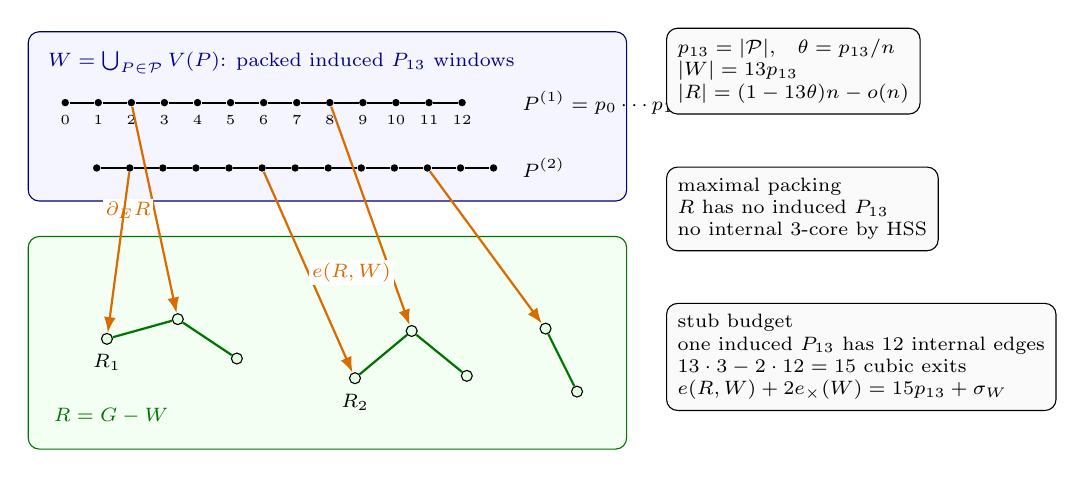
\begin{tikzpicture}[
win/.style={circle,fill=black,inner sep=0.95pt},
rv/.style={circle,draw,fill=green!10,inner sep=1.4pt},
stub/.style={-{Latex[length=2mm]},thick,orange!85!black},
redge/.style={thick,green!45!black},
box/.style={rectangle,rounded corners,draw,align=left,inner sep=4pt,fill=black!2},
every node/.style={font=\scriptsize}
]
\draw[rounded corners,fill=blue!4,draw=blue!45!black] (-4.75,0.80) rectangle (2.85,2.95);
\node[anchor=north west,blue!55!black] at (-4.62,2.82) {$W=\bigcup_{P\in\mathcal P}V(P)$: packed induced $P_{13}$ windows};
\foreach \i in {0,...,12} {
  \node[win] (p\i) at (-4.28+0.42*\i,2.05) {};
  \node[font=\tiny,below=1pt] at (-4.28+0.42*\i,2.05) {$\i$};
  \node[win] (q\i) at (-3.88+0.42*\i,1.22) {};
}
\draw[thick] (p0)--(p1)--(p2)--(p3)--(p4)--(p5)--(p6)--(p7)--(p8)--(p9)--(p10)--(p11)--(p12);
\draw[thick] (q0)--(q1)--(q2)--(q3)--(q4)--(q5)--(q6)--(q7)--(q8)--(q9)--(q10)--(q11)--(q12);
\node[anchor=west] at (1.40,2.05) {$P^{(1)}=p_0\cdots p_{12}$};
\node[anchor=west] at (1.40,1.22) {$P^{(2)}$};

\draw[rounded corners,fill=green!5,draw=green!45!black] (-4.75,-2.35) rectangle (2.85,0.35);
\node[anchor=south west,green!45!black] at (-4.55,-2.15) {$R=G-W$};
\node[rv,label=below:$R_1$] (r1) at (-3.75,-0.95) {};
\node[rv] (r2) at (-2.85,-0.70) {};
\node[rv] (r3) at (-2.10,-1.20) {};
\draw[redge] (r1)--(r2)--(r3);
\node[rv,label=below:$R_2$] (s1) at (-0.60,-1.45) {};
\node[rv] (s2) at (0.12,-0.85) {};
\node[rv] (s3) at (0.82,-1.42) {};
\draw[redge] (s1)--(s2)--(s3);
\node[rv] (t1) at (1.82,-0.82) {};
\node[rv] (t2) at (2.22,-1.62) {};
\draw[redge] (t1)--(t2);

\draw[stub] (p2)--node[left,fill=white,inner sep=1pt]{$\partial_E R$}(r2);
\draw[stub] (p8)--(s2);
\draw[stub] (q1)--(r1);
\draw[stub] (q5)--node[right,fill=white,inner sep=1pt]{$e(R,W)$}(s1);
\draw[stub] (q10)--(t1);

\node[box,anchor=west] at (3.35,2.45) {$p_{13}=|\mathcal P|$,\quad $\theta=p_{13}/n$\\
$|W|=13p_{13}$\\
$|R|=(1-13\theta)n-o(n)$};
\node[box,anchor=west] at (3.35,0.70) {maximal packing\\
$R$ has no induced $P_{13}$\\
no internal $3$-core by HSS};
\node[box,anchor=west] at (3.35,-1.18) {stub budget\\
one induced $P_{13}$ has $12$ internal edges\\
$13\cdot3-2\cdot12=15$ cubic exits\\
$e(R,W)+2e_\times(W)=15p_{13}+\sigma_W$};
\end{tikzpicture}%
}
\caption[Visual definition of the \(P_{13}\)-window remainder ledger]{Visual definition of the packed-window and remainder ledger.  The blue region is \(W=\bigcup_{P\in\mathcal P}V(P)\), where \(\mathcal P\) is a maximal vertex-disjoint family of induced \(P_{13}\) windows.  Black vertices and black edges are window vertices and their internal path edges; the displayed indices \(0,\ldots,12\) name the vertices of \(P^{(1)}=p_0\cdots p_{12}\).  The green region is the remainder \(R=G-W\); white vertices are remainder vertices, green edges are edges internal to \(R\), and \(R_1,R_2\) mark components of \(R\).  The packing size is \(p_{13}=|\mathcal P|\), its density is \(\theta=p_{13}/n\), \(|W|=13p_{13}\), and \(|R|=(1-13\theta)n-o(n)\).  Maximality of \(\mathcal P\) makes every component of \(R\) induced-\(P_{13}\)-free; the HSS theorem then forbids any internal subgraph of minimum degree at least \(3\) inside a component of \(R\).  Orange arrows are window--remainder incidences, counted by \(e(R,W)\) and by the oriented boundary ledger \(\partial_E R\).  Since each packed window is induced, \(G[W]\) has exactly \(12p_{13}\) path edges plus the cross-window edges counted by \(e_\times(W)\).  The exact degree-sum identity is \(e(R,W)+2e_\times(W)=15p_{13}+\sigma_W\), so every surplus unit on a window must be spent either as an additional window--remainder incidence or as two half-incidences in a cross-window join.}
\label{fig:p13-remainder-ledger}
\end{figure}

\begin{definition}[Positive deficiency and surplus]\label[definition]{def:deficiency-surplus}
For a subgraph $X\subseteq G$, define its positive deficiency by
\[
\defp(X)=\sum_{v\in V(X)}\max\{0,3-d_X(v)\}.
\]
Define the ambient surplus carried by vertices of $X$ by
\[
\sigma(X)=\sum_{v\in V(X)}\max\{0,d_G(v)-3\}.
\]
For the whole graph, write
\[
\sigma(G)=\sum_{v\in V(G)}(d_G(v)-3).
\]
Positive deficiency, not signed cubic charge, measures external degree demand: high-degree vertices inside $X$ cannot cancel the fact that vertices of internal degree below $3$ need outside incidences.
\end{definition}

\begin{definition}[Window--remainder surplus split]\label[definition]{def:window-remainder-surplus-split}
Let
\[
\sigma_W:=\sum_{w\in W}(d_G(w)-3),
\qquad
\sigma_R:=\sum_{v\in R}(d_G(v)-3).
\]
Since \(\delta(G)\ge3\), these sums are nonnegative,
\[
\sigma_R=\sigma(R),
\qquad
\sigma(G)=\sigma_W+\sigma_R.
\]
Let \(e_\times(W)\) be the number of edges of \(G\) whose endpoints lie in two
distinct packed \(P_{13}\)-windows.  The packed windows are induced, so the
edges of \(G[W]\) are exactly the \(12p_{13}\) path edges inside the windows
together with these \(e_\times(W)\) cross-window edges.
\end{definition}

\begin{lemma}[External-incidence supply for the $P_{13}$-free remainder]\label[lemma]{lem:stub-positive}
Assume \cref{def:near-cubic-spine}.
The $P_{13}$-free remainder satisfies
\[
\defp(R)\le e(R,W)\le15p_{13}+o(n)
\]
and hence
\[
\defp(R)-\sigma_R\le15p_{13}+o(n).
\]
Equivalently,
\[
\frac{\defp(R)-\sigma_R}{|R|}\le \frac{15\theta}{1-13\theta}+o(1).
\]
\end{lemma}

\begin{proof}
Since $\delta(G)\ge3$, every vertex $v\in R$ has $d_G(v)\ge3$, so $v$ is deficient in $R$ only because some of its incidences leave $R$.  Writing $d_G(v)=d_R(v)+e_v$, where $e_v$ is the number of edges from $v$ to $W=G-R$, and using $\max\{0,3-d_G(v)\}=0$,
\[
\max\{0,3-d_R(v)\}\le \max\{0,3-d_G(v)\}+e_v=e_v .
\]
Summing over $v\in R$,
\[
\defp(R)=\sum_{v\in R}\max\{0,3-d_R(v)\}\le\sum_{v\in R}e_v=e(R,W),
\]
the number of edges between $R$ and $W$.

It remains to bound $e(R,W)$ by the outside-incidence capacity of the windows.  Each $P\in\mathcal P$ is an \emph{induced} $P_{13}$, so the subgraph of $G$ on $V(P)$ has exactly its $12$ path edges.  The number of edges leaving $V(P)$ (to $R$ or to another window) equals the degree sum on $V(P)$ minus twice the internal edges:
\[
\sum_{w\in V(P)}d_G(w)-2\cdot12
=\Bigl(39+\sum_{w\in V(P)}(d_G(w)-3)\Bigr)-24
=15+\sigma(P),
\]
where $\sigma(P)=\sum_{w\in V(P)}(d_G(w)-3)$ is the surplus carried by $P$ and $39=13\cdot3$ is the cubic degree sum.  Every $R$--$W$ edge leaves some window, so summing over the $p_{13}$ windows,
\[
e(R,W)\le\sum_{P\in\mathcal P}\bigl(15+\sigma(P)\bigr)=15p_{13}+\sigma_W\le 15p_{13}+\sigma(G),
\]
where \(\sigma_W=\sum_{P\in\mathcal P}\sigma(P)\le\sigma(G)\) since the windows are vertex-disjoint and surplus is nonnegative.  Combining the two displays gives
\[
\defp(R)\le e(R,W)\le15p_{13}+\sigma(G).
\]
By \cref{def:near-cubic-spine}, $\sigma(G)=O(\sqrt n)=o(n)$, so
\[
\defp(R)\le e(R,W)\le15p_{13}+o(n).
\]
Since \(\sigma_R\ge0\), this implies
\[
\defp(R)-\sigma_R\le15p_{13}+o(n).
\]
Dividing by $|R|=(1-13\theta)n+o(n)$ and using $p_{13}=\theta n$ gives the normalized form.
\end{proof}

\begin{lemma}[Exact window-join identity]\label[lemma]{lem:exact-window-join-identity}
With notation as in \cref{def:window-remainder-surplus-split},
\[
e(R,W)+2e_\times(W)=15p_{13}+\sigma_W .
\]
\end{lemma}

\begin{proof}
Sum degrees over the window vertices.  Since \(|W|=13p_{13}\),
\[
\sum_{w\in W}d_G(w)=3|W|+\sigma_W=39p_{13}+\sigma_W .
\]
The same degree sum counts twice the edges internal to \(W\) and once the
edges from \(W\) to \(R\).  By
\cref{def:window-remainder-surplus-split}, the internal edges of \(G[W]\) are
the \(12p_{13}\) path edges inside the packed windows and the
\(e_\times(W)\) cross-window edges.  Hence
\[
39p_{13}+\sigma_W
=2(12p_{13}+e_\times(W))+e(R,W).
\]
Rearranging gives the identity.
\end{proof}

\begin{lemma}[Surplus-aware window-stub inequality]\label[lemma]{lem:surplus-aware-window-stub}
No near-cubic hypothesis is required for the following estimates:
\[
\defp(R)\le e(R,W)\le15p_{13}+\sigma_W
\]
and
\[
\defp(R)-\sigma_R\le15p_{13}+\sigma_W-\sigma_R .
\]
\end{lemma}

\begin{proof}
The proof of \cref{lem:stub-positive} gives the first inequality
\[
\defp(R)\le e(R,W)
\]
using only \(\delta(G)\ge3\).  By
\cref{lem:exact-window-join-identity},
\[
e(R,W)=15p_{13}+\sigma_W-2e_\times(W)\le15p_{13}+\sigma_W,
\]
because \(e_\times(W)\ge0\).  Subtracting \(\sigma_R\) from the first displayed
upper bound gives
\[
\defp(R)-\sigma_R\le15p_{13}+\sigma_W-\sigma_R .
\]
\end{proof}

\begin{corollary}[Boundary-incidence supply]\label[corollary]{cor:stub-boundary-supply}
Assume \cref{def:near-cubic-spine}.
The total positive deficiency of the $P_{13}$-free remainder satisfies
\[
\defp(R)\le15p_{13}+o(n).
\]
Equivalently,
\[
\frac{\defp(R)}{|R|}\le\tau_{\rm win}+o(1),
\qquad
\tau_{\rm win}=0.22817486846\ldots .
\]
\end{corollary}

\begin{proof}
The proof of \cref{lem:stub-positive} gives
\[
\defp(R)\le e(R,W)\le15p_{13}+\sigma(G).
\]
By \cref{def:near-cubic-spine}, $\sigma(G)=O(\sqrt n)=o(n)$.  Hence
$\defp(R)\le15p_{13}+o(n)$.  Dividing by
$|R|=(1-13\theta)n+o(n)$ and using
$\theta\le\theta_{\rm win}+o(1)$ from \cref{prop:p13-density} gives the
normalized form.
\end{proof}

\paragraph{Framework branch table.}
The packed-window remainder and deficiency supply close or route residuals as
follows.
\begin{longtable}{L{0.13\textwidth} L{0.19\textwidth} L{0.14\textwidth} L{0.14\textwidth} L{0.17\textwidth} L{0.17\textwidth}}
\FrameworkBranchTableHeader
Forced remainder
&
The maximal \(P_{13}\)-packing leaves \(R\).
&
Unpacked vertices.
&
Maximality of the packing.
&
Componentwise in \(R\).
&
\(R\) is \(P_{13}\)-free.
\\
\addlinespace
Internal \(3\)-core
&
A component of \(R\) has a subgraph of minimum degree at least \(3\).
&
No budget is available.
&
\cref{thm:p13free}.
&
One component at a time.
&
Gives a dyadic cycle.
\\
\addlinespace
Window incidence
&
Positive deficiency occurs in \(R\).
&
\(\defp(R)\).
&
Window--remainder stubs.
&
At most \(15\) cubic exits per packed window, plus surplus.
&
\(\defp(R)\le15p_{13}+o(n)\) by \cref{lem:stub-positive,cor:stub-boundary-supply}.
\\
\addlinespace
Surplus-adjusted supply
&
Remainder surplus is tracked separately.
&
\(\defp(R)-\sigma_R\).
&
The exact window-join identity.
&
The stub and cross-window partition.
&
\cref{lem:exact-window-join-identity,lem:surplus-aware-window-stub}.
\\
\bottomrule
\end{longtable}

\section{Curvature supply in the atom remainder}

For a component $C$ of $R$, define the number of internal length-two wedges by
\[
W_2(C)=\sum_{v\in V(C)}\binom{d_C(v)}2.
\]
Let
\[
W_2(R)=\sum_{C\subseteq R}W_2(C).
\]

\begin{lemma}[Wedge lower bound]\label[lemma]{lem:wedge-lower}
For every component $C$,
\[
W_2(C)\ge3|V(C)|-2\defp(C).
\]
In particular, under \cref{def:near-cubic-spine}, in the window-only
low-deficiency branch, where
$\defp(R)\le(\tau_{\rm win}+o(1))|R|$ with
$\tau_{\rm win}=0.22817486846\ldots$,
\[
W_2(R)\ge \omega_{\rm win}|R|-o(|R|),
\qquad
\omega_{\rm win}=2.54365026308\ldots .
\]
In the sharper high-entropy branch, where
$\defp(R)\le(0.21296321056\ldots+o(1))|R|$, this improves to
\[
W_2(R)\ge \omega |R|-o(|R|),
\qquad
\omega=2.57407357888\ldots .
\]
\end{lemma}

\begin{proof}
For a component $C$, let
\[
n_i=|\{v\in V(C):d_C(v)=i\}|\qquad(i\ge0).
\]
Then
\[
|V(C)|=\sum_{i\ge0}n_i,
\]
\[
\defp(C)=3n_0+2n_1+n_2,
\]
and
\[
W_2(C)=\sum_{i\ge0}\binom i2 n_i.
\]
A direct calculation gives
\[
W_2(C)-\bigl(3|V(C)|-2\defp(C)\bigr)
=3n_0+n_1+\sum_{i\ge3}\left(\binom i2-3\right)n_i\ge0.
\]
Thus
\[
W_2(C)\ge3|V(C)|-2\defp(C).
\]
Summing over the connected components $C$ of $R$, and using $\sum_C|V(C)|=|R|$ and $\sum_C\defp(C)=\defp(R)$ (within a component $d_C=d_R$, so the per-component deficiencies add up to $\defp(R)$),
\[
W_2(R)=\sum_{C\subseteq R}W_2(C)\ge 3|R|-2\defp(R).
\]
In the near-cubic window-only low-deficiency branch,
\cref{cor:stub-boundary-supply} gives
\[
\defp(R)\le(\tau_{\rm win}+o(1))|R|,
\]
with
$\tau_{\rm win}=0.22817486846\ldots$.  Therefore
\[
W_2(R)\ge
\left(3-2\cdot0.22817486846\ldots-o(1)\right)|R|
=(\omega_{\rm win}-o(1))|R|,
\]
where
\[
\omega_{\rm win}=3-2\cdot0.22817486846\ldots=2.54365026308\ldots .
\]
If the sharper high-entropy cap is available, then
$\defp(R)/|R|\le0.21296321056\ldots+o(1)$.  Substituting this value into
\(W_2(R)\ge3|R|-2\defp(R)\) gives
\[
W_2(R)\ge\left(3-2\cdot0.21296321056\ldots-o(1)\right)|R|=(\omega-o(1))|R|,
\]
where the constant is
\[
\omega=3-2\cdot0.21296321056\ldots=2.57407357888\ldots.
\]
\end{proof}

\paragraph{Framework branch table.}
The curvature-supply section instantiates the framework table as follows.
\begin{longtable}{L{0.13\textwidth} L{0.19\textwidth} L{0.14\textwidth} L{0.14\textwidth} L{0.17\textwidth} L{0.17\textwidth}}
\FrameworkBranchTableHeader
Component wedge count
&
\(C\) is a component of \(R\).
&
\(W_2(C)\).
&
Positive deficiency.
&
The degree-count identity by internal degree.
&
\(W_2(C)\ge3|V(C)|-2\defp(C)\) by \cref{lem:wedge-lower}.
\\
\addlinespace
Window-only demand
&
\(\defp(R)\le(\tau_{\rm win}+o(1))|R|\).
&
Linear wedge supply.
&
The window-stub deficiency cap.
&
Summation over components.
&
\(W_2(R)\ge\omega_{\rm win}|R|-o(|R|)\).
\\
\addlinespace
High-entropy demand
&
The sharper high-entropy deficiency cap is available.
&
Larger wedge supply.
&
The high-entropy density cap.
&
The same degree-count identity.
&
\(W_2(R)\ge\omega|R|-o(|R|)\).
\\
\bottomrule
\end{longtable}

\section{Curvature rank and rank forcing}

\begin{definition}[Curvature target-rank]\label[definition]{def:curvature-target-rank}
For an atom $C$, let $\mathcal W_2(C)$ be the set of raw internal length-two
curvature tests in $C$.  A subfamily
$\mathcal A\subseteq\mathcal W_2(C)$ \emph{survives} an admissible rank quotient
$q$ when $q$ is label-injective on $\mathcal A$ in the sense of
\cref{def:exact-response-profile}.  It survives the admissible quotient system
when it survives every functional admissible rank quotient of
\cref{def:admissible-rank-quotient,def:functional-rank-quotient}.  The
curvature target-rank $r_\Omega(C)$ is the maximum size of such a surviving
subfamily.  Equivalently, it is the maximum size of an independently
target-testable subfamily after all target-complete identifications with proper
support have been imposed.  For the atom remainder $R$, let $r_\Omega(R)$ be
the target rank of the union of the raw atom curvature tests.  Closed
whole-graph data are evaluated in the exact profile
$\rho_\varnothing^{\rm ex}(G)$, so the empty context by itself creates no
curvature-rank identifications.
\end{definition}

\begin{definition}[Curvature target-dependence]\label[definition]{def:curvature-target-dependence}
Let \(\mathcal A\) be a finite family of curvature tests.  A
\emph{target-dependence} in \(\mathcal A\) is a pair
\[
(a,\mathcal B),\qquad a\in\mathcal A,\quad
\mathcal B\subseteq\mathcal A\setminus\{a\},
\]
such that a functional admissible rank quotient of the exact response profile
determines the target-response value of \(a\) from the target-response vector
on \(\mathcal B\).  In this definition, the phrase ``adjoining \(a\) to
\(\mathcal B\) does not increase the number of target-complete states'' means
precisely that the projection to the \(\mathcal B\)-coordinates is the graph of
the function determining the \(a\)-coordinate under the admissible quotient.
The dependence is
\emph{proper} when this determination is not a tautological equality of the
local coordinate \(a\) with one of the coordinates in \(\mathcal B\).

A \emph{determination certificate} for \((a,\mathcal B)\) is a tuple
\[
\mathfrak c=(X,T,q,\mathcal P)
\]
with the following data.
\begin{enumerate}[label=(\alph*), leftmargin=2.2em]
\item \(X\subseteq G\) is a connected \(T\)-boundaried support carrying all
coordinates in \(\{a\}\cup\mathcal B\).
\item \(q:\rho_T^{\rm ex}(X)\to Q\) is a functional admissible rank quotient.
\item For any two realizations of \(\rho_T^{\rm ex}(X)\) with the same
\(q\)-image on the coordinates of \(\mathcal B\), the \(q\)-image of \(a\) is
the same.  Equivalently, the \(q\)-value of \(a\) is a function of the
\(q\)-value vector on \(\mathcal B\).
\item \(\mathcal P\) is the finite set of declared paths, boundary incidences,
window segments, or connector incidences recorded by the certificate as the
support data for the context-universal determination.
\end{enumerate}
Here a realization means a \(T\)-boundaried support whose exact response profile
maps to the same quotient data \(Q\) under \(q\).  The \emph{support} of
\(\mathfrak c\) is the lexicographically first smallest connected subgraph of
\(G\) containing the declared supports of \(a\), of all coordinates in
\(\mathcal B\), and of every member of \(\mathcal P\).  The support of
\((a,\mathcal B)\) is the support of a certificate with minimal support.  A
target-dependence is \emph{inclusion-minimal} if no proper connected subsupport
carries a proper target-dependence with the same determined coordinate.
\end{definition}

\begin{lemma}[Target-rank circuit extraction]\label[lemma]{lem:target-rank-circuit}
Let $\mathcal A$ be a finite family of declared coordinates evaluated under the
functional admissible quotients of a fixed exact response profile.  If a subfamily
$\mathcal I\subseteq\mathcal A$ is maximal among subfamilies that survive every
functional admissible rank quotient and $a\in\mathcal A\setminus\mathcal I$,
then there is a subfamily $\mathcal B\subseteq\mathcal I$ such that
\((a,\mathcal B)\) is a target-dependence in the sense of
\cref{def:curvature-target-dependence}.  In particular, if no proper
target-dependence exists among the coordinates of $\mathcal A$, then the whole
family $\mathcal A$ survives every functional admissible rank quotient and is
independently target-testable in the rank sense of
\cref{def:curvature-target-rank}.
\end{lemma}

\begin{proof}
Since $\mathcal I$ is maximal for survival, $\mathcal I\cup\{a\}$ fails to
survive some functional admissible rank quotient
\[
q:\rho_T^{\rm ex}(X)\to Q.
\]
The subfamily \(\mathcal I\) survives \(q\).  Hence the failure of
label-injectivity for \(\mathcal I\cup\{a\}\) involves \(a\).  By
\cref{def:functional-rank-quotient}, the quotient \(q\) is functional on
\(\mathcal A\).  Therefore there is a finite subfamily
\(\mathcal B\subseteq\mathcal I\) whose \(q\)-image vector determines the
\(q\)-image of \(a\).  Choose such a subfamily inclusion-minimal.  If \(a\) is
sent to a single quotient value after the quotient forgets its separate label,
then \(\mathcal B=\varnothing\).  If \(a\) is identified with a coordinate of
\(\mathcal I\), then the functional certificate may be taken with
\(\mathcal B=\{b\}\) for such a coordinate \(b\).  The quotient \(q\), together
with the declared supports of \(a\), of \(\mathcal B\), and of the finitely many
coordinates used by \(q\), is a determination certificate.

If the dependence is tautological, then $a$ is the same local coordinate as an
element of $\mathcal B$.  Exact coordinate labels keep distinct declared raw
coordinates distinct, so a rank loss among distinct raw curvature coordinates
yields a proper dependence.  The contrapositive gives the final assertion.
\end{proof}

If \(r_\Omega(C)<|\mathcal W_2(C)|\), then some coordinate outside a maximal
independently target-testable subfamily is target-dependent on that subfamily in
the sense of \cref{def:curvature-target-dependence,lem:target-rank-circuit}.
This is the only meaning of ``dependence'' used below.

\begin{lemma}[Localization of curvature dependence]\label[lemma]{lem:curvature-dependence-routing}
Let $C$ be a proper atom and let $\mathcal W_2(C)$ be its raw curvature tests.  If
\[
r_\Omega(C)<|\mathcal W_2(C)|,
\]
then some target-dependence among raw curvature tests falls into one of the following cases:
\begin{enumerate}[label=(\roman*)]
\item a target-defective quotient;
\item an admissible nontrivial target-complete compression of a proper atom;
\item a target-dependence that becomes valid only after adjoining a connected support $Z\supsetneq C$.
\end{enumerate}
\end{lemma}

\begin{proof}
A strict rank drop means that some raw curvature test is target-dependent on
the others in the sense of
\cref{def:curvature-target-dependence,lem:target-rank-circuit}.  Choose a
determination certificate with inclusion-minimal connected support.  The
certificate has an admissible quotient \(q\) and a finite support set
\(\mathcal P\).  Either the determination certified by \(q\) fails for some
\(T\)-boundaried outside context, or it is context-universal.  In the
context-universal case, the connected support of the certificate either equals
\(C\) or strictly contains \(C\).  These alternatives are mutually exclusive and
exhaust all certificates:
\begin{enumerate}[label=(\roman*)]
\item if the determination fails for some outside context, it is not preserved under context-universality and hence is a target-defective quotient;
\item if it holds for every outside context already with support $C$, then \(q\) is a target-complete rank-reducing quotient of the proper atom \(C\).  Since \(q\) is admissible, \cref{def:admissible-rank-quotient} supplies a strictly smaller proper representative.  Thus this case is a nontrivial target-complete compression of \(C\);
\item otherwise it holds for every outside context but only once additional structure outside $C$ is adjoined; taking an inclusion-minimal connected such support yields a connected $Z\supsetneq C$.
\end{enumerate}
\end{proof}


\begin{lemma}[Separated wedges are tested by disjoint contexts]\label[lemma]{lem:separated-testers}
Let $u,v\in V(R)$ have identical rooted radius-$r$ neighbourhood types,
$B_r(u)\cong B_r(v)$, and suppose the closed balls $\overline B_r(u)$ and
$\overline B_r(v)$ are vertex-disjoint.  Let $w(u),w(v)$ be the corresponding
internal length-two wedge tests at the two roots.  Then any target tester
separating $w(u)$ from $w(v)$ has its support in the complement of
$\overline B_r(u)\cup\overline B_r(v)$.  Consequently, any quotient identifying
$w(u)$ with $w(v)$ is either context-universal or target-defective.
\end{lemma}

\begin{proof}
A target tester for a wedge coordinate is a boundaried context glued to the
support of that wedge.  The wedge itself is an internal length-two path at the
root of its radius-$r$ ball.  Any closure witnessing a dyadic target that is not
already internal to the ball must leave the ball through its boundary; if the
witness stayed wholly inside the ball, the ball would already contain a target
cycle, contrary to internal target-safety of the remainder.  Hence every tester
that separates the two wedge coordinates is supported outside the corresponding
closed balls.

Since the rooted balls are isomorphic and vertex-disjoint, the two local wedge
states have identical internal data and identical boundary degree profiles.  If
an outside context distinguishes them, then the identification fails the
context-universality condition of target-completeness and is target-defective.
If no outside context distinguishes them, the identification is
context-universal.  These are the only two possibilities.
\end{proof}

\begin{lemma}[Proper delocalization supports are forbidden]\label[lemma]{lem:proper-smearing}
Let $C\subsetneq G$ be a proper atom.  Suppose a target-dependence among curvature tests of $C$ becomes target-complete only after adjoining an inclusion-minimal connected support $Z\supseteq C$.  If
\[
Z\subsetneq G,
\]
then the dependence is impossible.
\end{lemma}

\begin{proof}
Regard $Z$ as a boundaried graph with boundary
\[
\partial Z=\{v\in V(Z):v\text{ is incident with an edge of }G-Z\}.
\]
The response state of $Z$ includes its boundary degree profile and all target-response data inherited from $C$.  Since $Z\subsetneq G$, it is a proper boundaried support.  If the dependence fails against some outside $\partial Z$-context, it is target-defective.  If it succeeds against every outside context, it is a nontrivial target-complete compression of the proper support $Z$, forbidden by \cref{cor:uncompressible}.
\end{proof}

\begin{definition}[Repair-network terminology]\label[definition]{def:repair-network-terms}
Let \(Z\) be the support of a determination certificate.  A vertex of \(Z\) is a
\emph{passive degree-two subdivision vertex} if it has degree \(2\) in \(Z\), is
not a boundary vertex of \(Z\), and is not contained in the declared support of
any coordinate, path endpoint, packed-window incidence, trace incidence, fan
decoration, or carrier used by the certificate.  Such a vertex records only an
unlabelled subdivision of a response path.

After deleting the original coordinate supports of the dependence from \(Z\),
each remaining connected component that meets the deleted part only in boundary
leaves is a \emph{delayed compensation component}.  If such a component has
\(p\) boundary leaves and all non-leaf vertices have degree \(3\) except for
the recorded surplus contribution \(\sigma_Z\), then it is a
\emph{\(1\)--\(3\) repair network up to surplus}.  Its internal vertex count is
denoted \(s\), and its cycle rank is denoted \(\beta_Z\).
\end{definition}

\begin{lemma}[Enlarged delocalization supports are repair networks]\label[lemma]{lem:smearing-support-repair}
Let $Z$ be a connected support on which a formerly nonlocal dependence becomes internal.  Suppose $Z$ is target-safe, contains no proper subgraph of minimum degree at least $3$, and has no passive degree-two subdivision vertices.  Then each delayed compensation component of $Z$ is a $1$--$3$ repair network up to surplus.  More precisely, if such a connected component has $p$ boundary leaves, $s$ internal vertices, cycle rank $\beta_Z$, and surplus $\sigma_Z$, then
\[
s=p-2+2\beta_Z-\sigma_Z.
\]
\end{lemma}

\begin{proof}
The component has $s$ internal vertices and $p$ boundary leaves, hence $s+p$ vertices in all.  Let $e$ be the number of edges joining two internal vertices; each boundary leaf is attached by a single edge, so the component has $e+p$ edges in total.  Each internal vertex has degree $3$ up to its surplus, so the internal vertices contribute $3s+\sigma_Z$ to the degree sum, and each of the $p$ leaves has degree $1$.  The handshake identity $\sum_v d(v)=2\cdot(\text{number of edges})$ therefore reads
\[
(3s+\sigma_Z)+p=2(e+p),
\]
which simplifies to
\[
3s+\sigma_Z=2e+p. \tag{$\dagger$}
\]
The component is connected, so its cycle rank is
\[
\beta_Z=(e+p)-(s+p)+1=e-s+1,\qquad\text{equivalently}\qquad e=s-1+\beta_Z.
\]
Substituting $e=s-1+\beta_Z$ into $(\dagger)$ gives $3s+\sigma_Z=2(s-1+\beta_Z)+p=2s-2+2\beta_Z+p$, and solving for $s$ yields
\[
s=p-2+2\beta_Z-\sigma_Z. \qedhere
\]
\end{proof}

\begin{lemma}[No silent global delocalization]\label[lemma]{lem:no-silent-global-smearing}
Let a curvature target-dependence have inclusion-minimal connected support equal
to the whole graph $G$.  Then any attempted rank-reducing quotient is either
target-defective, represented by a strictly smaller admissible closed
representative, or exact on the raw curvature labels.  In particular, a
target-complete
whole-graph dependence cannot silently reduce atom curvature rank.
\end{lemma}

\begin{proof}
Let $q:\rho_\varnothing^{\rm ex}(G)\to Q$ be the quotient of the closed exact
response profile which witnesses the proposed dependence in the sense of
\cref{def:curvature-target-dependence}.  Since the support is all of $G$, the
boundary is empty and the only actual outside context is the empty graph.
\Cref{def:admissible-rank-quotient} is the rule that prevents this empty context
from identifying all coordinates vacuously.

If the attempted quotient is not target-complete, then it is target-defective
by definition and cannot witness a target-dependence.  This is the
target-defect exit used elsewhere in the proof, so it is not a surviving global
rank reduction.

Assume next that $q$ is target-complete and has a strictly smaller admissible
closed representative $G_q$ in the sense of
\cref{def:closed-quotient-representative}.  Thus \(G_q\) is finite and simple,
\(\delta(G_q)\ge3\), and
\(\profile_\varnothing(G_q)\subseteq\profile_\varnothing(G)\).  If \(G_q\)
contained a dyadic cycle, then
the empty \(\varnothing\)-boundaried context would belong to
\(\profile_\varnothing(G_q)\).  The same empty context does not belong to
\(\profile_\varnothing(G)\), because \(G\) has no dyadic cycle.  This would
contradict \(\profile_\varnothing(G_q)\subseteq\profile_\varnothing(G)\).
Hence \(G_q\) has no dyadic cycle.  Thus \(G_q\) is a strictly smaller
counterexample, contradicting the lexicographic minimality of \(G\).

It remains that $q$ is target-complete and has no smaller closed representative.
By the closed clause in \cref{def:admissible-rank-quotient}, such a quotient is
label-injective on the raw curvature coordinates of
\(\rho_\varnothing^{\rm ex}(G)\).  Therefore it neither forgets a raw curvature
coordinate nor identifies two distinct raw curvature coordinates.  It can record
exact global response data, but it is not curvature-rank-reducing.  This
contradicts the assumption that the whole-graph dependence reduced
\(r_\Omega\).
\end{proof}

\begin{lemma}[Forcing of full curvature rank]\label[lemma]{lem:full-rank}
In a minimal counterexample,
\[
r_\Omega(R)\ge W_2(R)-o(W_2(R)).
\]
\end{lemma}

\begin{proof}
If not, then
\[
r_\Omega(R)<W_2(R)-o(W_2(R)).
\]
By \cref{lem:target-rank-circuit}, a rank loss among the raw curvature
coordinates gives a proper target-dependence.  Choose such a dependence with a
determination certificate of inclusion-minimal connected support, and call that
support $Z$.  The minimality of $Z$ gives two possibilities.

First suppose $Z\subsetneq G$.  Regard $Z$ as a proper boundaried atom with
boundary $\partial Z$.  If the dependence is already visible inside a smaller
proper atom $C\subseteq Z$, then \cref{lem:curvature-dependence-routing}
applies to $C$.  Its three alternatives are respectively: a target-defective
quotient, a target-complete compression of a proper atom, or a dependence that
requires an enlarged connected support.  The first is excluded by the
definition of target-completeness; the second is excluded by
\cref{cor:uncompressible}; and the third, because the enlarged support is still
proper in $G$, is excluded by \cref{lem:proper-smearing}.  If no smaller
$C\subsetneq Z$ carries the dependence, then $Z$ itself is the first proper
support on which it becomes target-complete, and \cref{lem:proper-smearing}
again excludes it.

It remains that the inclusion-minimal support is $Z=G$.  Then the dependence
becomes context-universal only globally.  By
\cref{lem:no-silent-global-smearing}, such a global dependence either creates a
target cycle, creates a replacement, or contributes exact non-identifying
global response data.  The first two alternatives contradict the counterexample
condition and minimality; the third does not identify two distinct local
curvature tests and hence is not a proper target-dependence.  Thus no proper
target-dependence survives.  By \cref{lem:target-rank-circuit}, the raw
curvature tests have no admissible rank loss.  Hence
\[
r_\Omega(R)=W_2(R),
\]
which implies the stated weaker bound
$r_\Omega(R)\ge W_2(R)-o(W_2(R))$.
\end{proof}

\begin{corollary}[Forced curvature cost]\label[corollary]{cor:forced-curvature-cost}
Assume \cref{def:near-cubic-spine}.
Any surviving residual pays at least
\[
c_\Omega r_\Omega(R)
\ge
K_{\mathrm{win}} |R|-o(|R|),
\]
where
\[
K_{\mathrm{win}}=c_\Omega\omega_{\mathrm{win}}=5.82298307395\ldots .
\]
In the sharper high-entropy low-deficiency branch this improves to
\[
c_\Omega r_\Omega(R)\ge K|R|-o(|R|),
\]
where
\[
K=c_\Omega\omega=5.89262883286\ldots .
\]
\end{corollary}

\begin{proof}
This follows from \cref{lem:full-rank,lem:wedge-lower} and the definitions of
$K_{\mathrm{win}}$ and $K$.
\end{proof}

\begin{remark}[Provenance of the curvature constant]\label[remark]{rem:curvature-provenance}
The two ingredients of \cref{cor:forced-curvature-cost} play distinct roles.
The \emph{independence} of the remainder curvature tests---that they realize
full target-rank (\cref{lem:full-rank})---is forced by the routing of
\cref{lem:curvature-dependence-routing}: any dependence among the tests would
be a target-defective quotient, a target-complete compression of a proper atom
(excluded by \cref{cor:uncompressible}), or a delocalization.  Proper
delocalization is excluded by \cref{lem:proper-smearing}; whole-graph
delocalization is excluded by the closed exact-profile argument in
\cref{lem:no-silent-global-smearing}.  Thus each route is unavailable in the
main spine.  The \emph{value} $c_\Omega$, by contrast, enters
through the window-only constant $K_{\rm win}=c_\Omega\omega_{\rm win}$ and
through the sharper high-entropy constant $K=c_\Omega\omega$ in the finite-size
threshold $\Theta(n)$ of \cref{def:Theta}.  As \cref{rem:closure-robust}
records, the closure outside the explicit residuals does not depend on the
exact value of $c_\Omega$; what the routing supplies is the independence of the
curvature cost, not its size.
\end{remark}

\begin{figure}[t]
\centering
\resizebox{0.98\textwidth}{!}{%
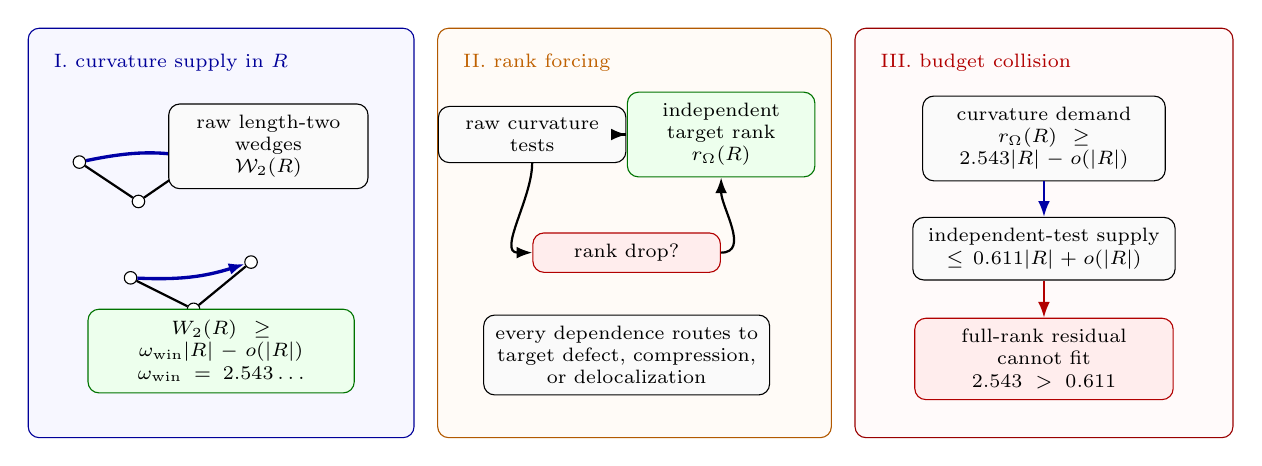
\begin{tikzpicture}[
pt/.style={circle,draw,fill=white,inner sep=1.6pt},
wedge/.style={-{Latex[length=2mm]},very thick,blue!65!black},
box/.style={rectangle,rounded corners,draw,fill=black!2,align=center,inner sep=4pt,text width=2.55cm},
good/.style={rectangle,rounded corners,draw=green!45!black,fill=green!7,align=center,inner sep=4pt,text width=2.55cm},
bad/.style={rectangle,rounded corners,draw=red!70!black,fill=red!7,align=center,inner sep=4pt,text width=2.55cm},
arr/.style={-{Latex[length=2mm]},thick},
every node/.style={font=\scriptsize}
]
\draw[rounded corners,fill=blue!3,draw=blue!60!black] (-7.55,-2.65) rectangle (-2.65,2.55);
\draw[rounded corners,fill=orange!3,draw=orange!70!black] (-2.35,-2.65) rectangle (2.65,2.55);
\draw[rounded corners,fill=red!2,draw=red!60!black] (2.95,-2.65) rectangle (7.75,2.55);
\node[anchor=north west,blue!60!black] at (-7.35,2.35) {I. curvature supply in \(R\)};
\node[anchor=north west,orange!75!black] at (-2.15,2.35) {II. rank forcing};
\node[anchor=north west,red!70!black] at (3.15,2.35) {III. budget collision};

\node[pt] (a) at (-6.90,0.85) {};
\node[pt] (b) at (-6.15,0.35) {};
\node[pt] (c) at (-5.35,0.90) {};
\node[pt] (d) at (-6.25,-0.62) {};
\node[pt] (e) at (-5.45,-1.02) {};
\node[pt] (f) at (-4.72,-0.42) {};
\draw[thick] (a)--(b)--(c);
\draw[thick] (d)--(e)--(f);
\draw[wedge] (a) to[bend left=10] (c);
\draw[wedge] (d) to[bend right=10] (f);
\node[box,text width=2.25cm] at (-4.50,1.05) {raw length-two\\wedges\\\(\mathcal W_2(R)\)};
\node[good,text width=3.10cm] at (-5.10,-1.55) {\(W_2(R)\ge\omega_{\rm win}|R|-o(|R|)\)\\\(\omega_{\rm win}=2.543\ldots\)};

\node[box,text width=2.10cm] (raw) at (-1.15,1.20) {raw curvature\\tests};
\node[good,text width=2.10cm] (rank) at (1.25,1.20) {independent\\target rank\\\(r_\Omega(R)\)};
\draw[arr] (raw)--(rank);
\node[bad,text width=2.10cm] (drop) at (0.05,-0.30) {rank drop?};
\draw[arr] (raw.south) to[out=-90,in=180] (drop.west);
\draw[arr] (drop.east) to[out=0,in=-90] (rank.south);
\node[box,text width=3.35cm] at (0.05,-1.60) {every dependence routes to\\target defect, compression,\\or delocalization};

\node[box,text width=2.80cm] (demand) at (5.35,1.15) {curvature demand\\\(r_\Omega(R)\ge2.543|R|-o(|R|)\)};
\node[box,text width=3.05cm] (supply) at (5.35,-0.25) {independent-test supply\\\(\le0.611|R|+o(|R|)\)};
\draw[arr,blue!65!black] (demand)--(supply);
\node[bad,text width=3.00cm] (collision) at (5.35,-1.65) {full-rank residual\\cannot fit\\\(2.543>0.611\)};
\draw[arr,red!70!black] (supply)--(collision);
\end{tikzpicture}%
}
\caption[Visual proof of the curvature supply--budget squeeze]{Visual proof of the curvature supply--budget squeeze.  Panel I shows the \(P_{13}\)-free remainder \(R\) producing raw internal length-two wedge tests; the wedge lower bound gives \(W_2(R)\ge\omega_{\rm win}|R|-o(|R|)\), with \(\omega_{\rm win}=2.543\ldots\) on the window-only branch.  Panel II shows the rank-forcing step: if the raw tests did not survive as target-rank, a dependence would route to target defect, proper compression, or delocalization, all of which are closed in the minimal counterexample.  Thus \(r_\Omega(R)\) is linear in \(W_2(R)\).  Panel III records the resulting collision with the independent-test budget: the full-rank branch demands at least \(2.543|R|-o(|R|)\) tests, while the supply side has capacity at most \(0.611|R|+o(|R|)\).}
\label{fig:curvature-budget-squeeze}
\end{figure}

\paragraph{Framework branch table.}
The curvature-rank forcing section closes the rank-drop alternatives by the
following table.
\begin{longtable}{L{0.13\textwidth} L{0.19\textwidth} L{0.14\textwidth} L{0.14\textwidth} L{0.17\textwidth} L{0.17\textwidth}}
\FrameworkBranchTableHeader
Rank drop
&
\(r_\Omega(R)<W_2(R)-o(W_2(R))\).
&
A dependent curvature coordinate.
&
The target-dependence route.
&
A finite functional circuit.
&
\cref{lem:target-rank-circuit,lem:curvature-dependence-routing}.
\\
\addlinespace
Proper support
&
The dependence localizes in \(Z\subsetneq G\).
&
The support profile.
&
Replacement or target defect.
&
The proper boundary profile.
&
\cref{lem:proper-smearing}.
\\
\addlinespace
Whole graph
&
The dependence delocalizes to all of \(G\).
&
The closed exact profile.
&
Closed representative minimality.
&
The empty-boundary exactness rule.
&
\cref{lem:no-silent-global-smearing}.
\\
\addlinespace
Full rank
&
All rank-drop alternatives are excluded.
&
Raw wedge tests.
&
Curvature target rank.
&
All but \(o(W_2)\) tests.
&
\cref{lem:full-rank,cor:forced-curvature-cost}.
\\
\bottomrule
\end{longtable}


\section{Per-vertex remainder entropy and two-budget routing}

Throughout this section, $R$ is the $P_{13}$-free remainder of the minimal counterexample, with $|R|=(1-13\theta)n-o(n)$.  The aim is to make the entropy branch explicit: the $n\log n$ skeleton budget and the linear forced curvature cost are used in disjoint regimes.

\begin{definition}[Per-vertex skeleton entropy of the remainder]\label[definition]{def:remainder-entropy}
Let $\mathcal G(R)$ be the set of labelled simple graphs on the fixed vertex set $V(R)$ satisfying the already imposed remainder constraints: subcubicity on the atom part, componentwise $P_{13}$-freeness, no internal $3$-core, and positive net-deficiency density at most the current cap.  Define
\[
\eta(R)=\frac{\log_2|\mathcal G(R)|}{|R|}.
\]
\end{definition}

\begin{lemma}[Dominant local type in the low-entropy branch]\label[lemma]{lem:dominant-type}
Fix $r\ge1$.  Suppose the radius-$r$ local-type coordinate of the remainder is structurally repetitive, in the sense that
\[
\log_2\bigl|\{\,(B_r(v))_{v\in V(R)}\,\}\bigr|=o(|R|),
\]
i.e. the number of realizable radius-$r$ type vectors is subexponential in $|R|$.  Then for every $\varepsilon>0$ a single rooted radius-$r$ type covers all but at most $\varepsilon|R|$ vertices of $R$, for all large $n$.  This hypothesis holds whenever the remainder is in the low-entropy regime $\eta(R)<\frac1{10}\log_2 n$ of \cref{def:remainder-entropy} \emph{and} the local-type coordinate carries a vanishing fraction of the total skeleton entropy.
\end{lemma}

\begin{proof}
There are only finitely many rooted subcubic radius-$r$ types; call the number
$t=t(r)$, a constant independent of $n$.  Suppose, for contradiction, that no
single type covered a $(1-\varepsilon)$-fraction of $V(R)$.  Then the empirical
type distribution $\pi=(\pi_1,\dots,\pi_t)$ over the $t$ types satisfies
$\max_a\pi_a\le1-\varepsilon$, so its Shannon entropy obeys
$H(\pi)\ge h(\varepsilon)>0$, where
$h(\varepsilon)=-\varepsilon\log_2\varepsilon-(1-\varepsilon)\log_2(1-\varepsilon)$
is the binary entropy function.  The labelled remainder class is closed under
relabeling of the fixed vertex set $V(R)$, and the radius-$r$ type vector is a
canonical labelled coordinate.  Therefore every permutation of one realized
type vector with empirical distribution $\pi$ is again realized by a relabelled
graph in the same class.  Distinct assignments of types to the labelled
vertices give distinct type vectors, so the number of type vectors with
empirical distribution $\pi$ is at least the multinomial coefficient, which by
Stirling's approximation satisfies
\[
\binom{|R|}{\pi_1|R|,\dots,\pi_t|R|}=2^{\,H(\pi)|R|-o(|R|)}\ge 2^{\,h(\varepsilon)|R|-o(|R|)} .
\]
Thus the number of realizable type vectors is $2^{\Theta(|R|)}$, exponential in $|R|$, contradicting the hypothesis that it is subexponential.  Hence some rooted radius-$r$ type covers a $(1-\varepsilon)$-fraction of $V(R)$.
\end{proof}

\begin{remark}\label[remark]{rem:cheap-regime-link}
The structural-repetitiveness hypothesis of \cref{lem:dominant-type} is
stronger than the single-scalar low-entropy regime
$\eta(R)<\frac1{10}\log_2 n$.  The radius-$r$ type coordinate is one canonical
coordinate of the remainder skeleton, so its bit-content is bounded by
$\eta(R)|R|$.  When that coordinate is $o(|R|)$ the lemma applies.  When it is
not $o(|R|)$ but the total remainder entropy is still below
$\frac1{10}|R|\log_2 n$, no dominance conclusion is asserted here; that
nonrepetitive low-entropy case is passed unchanged to the large-budget
net-charge analysis, which is independent of the precise curvature-rank
fraction by \cref{rem:closure-robust}.
\end{remark}

\begin{lemma}[Dominant type forces independent curvature translates]\label[lemma]{lem:translates-independent}
Suppose a rooted radius-$r$ type with $r\ge2$ occurs on all but $o(|R|)$
vertices of $R$ and contains an internal length-two wedge at its root.  Then
\[
r_\Omega(R)\ge c_r|R|-o(|R|)
\]
for a constant $c_r>0$ depending only on $r$.
\end{lemma}

\begin{proof}
Let $D\subseteq V(R)$ be the set of vertices carrying the dominant rooted
radius-$r$ type, so $|D|\ge|R|-o(|R|)$.  Subcubicity bounds each closed
radius-$r$ ball by
\[
|\overline B_r(v)|\le 1+3(2^r-1),
\]
a constant depending only on $r$.  Greedily choose a maximal subset
$S\subseteq D$ whose members are pairwise at distance greater than $2r$; then
the closed balls $\{\overline B_r(u):u\in S\}$ are pairwise vertex-disjoint.  By
maximality every vertex of $D$ lies within distance $2r$ of some $u\in S$, and
each ball of radius $2r$ has at most
\[
b'=1+3(2^{2r}-1)
\]
vertices.  Hence
\[
|S|\ge |D|/b'\ge |R|/b'-o(|R|).
\]
Each ball carries one internal length-two wedge at its root, so these give at
least \(|S|\) raw curvature tests.  Hence \(W_2(R)\ge |S|\).  Also
subcubicity gives \(W_2(R)\le 3|R|\), because a vertex of degree at most \(3\)
is the center of at most three unordered length-two wedges.  By
\cref{lem:full-rank},
\[
r_\Omega(R)\ge W_2(R)-o(W_2(R)).
\]
Since \(W_2(R)\ge |S|\ge |R|/b'-o(|R|)\), the error term is \(o(|R|)\), and
\[
r_\Omega(R)\ge |S|\ge |R|/b'-o(|R|).
\]
Take $c_r=1/b'$.
\end{proof}

\begin{remark}[A positive fraction of independent tests suffices]\label[remark]{rem:positive-fraction}
The separated-translate construction already yields independent wedge tests on a positive fraction of the remainder, $|S|\ge|R|/b'-o(|R|)$ with $b'$ a constant.  For the only downstream use---the forced cost of \cref{cor:forced-curvature-cost} feeding the threshold $\Theta(n)$---any positive linear rank $r_\Omega(R)\ge c|R|$ supplies a positive forced cost $c\,c_\Omega|R|$, and by \cref{rem:closure-robust} the closure outside the explicit residuals holds for every nonnegative value of that cost.  The conclusion is therefore insensitive to the precise rank fraction: full rank is the sharpest form, but a positive fraction is all that the remainder of the argument consumes.
\end{remark}

\begin{proposition}[Two-budget routing]\label[proposition]{prop:two-budget}
Assume \cref{def:near-cubic-spine}.
Let $R$ be the $P_{13}$-free remainder of a minimal counterexample and let $\eta(R)$ be its per-vertex skeleton entropy (\cref{def:remainder-entropy}).  Exactly one of the following holds.
\begin{enumerate}[label=(\alph*)]
\item \textbf{High-entropy branch: $\eta(R)\ge\frac1{10}\log_2 n$.}  The remainder then contributes at least
\[
\frac{|R|}{10}\log_2 n
\]
bits, and \cref{lem:p13-window-package} together with the remainder accounting
gives the packing bound of \cref{prop:p13-density}.
\item \textbf{Structurally repetitive low-entropy branch:}
$\eta(R)<\frac1{10}\log_2 n$ and the radius-$2$ local-type coordinate has
$o(|R|)$ bit-content.  Then \cref{lem:dominant-type} yields a dominant
radius-$2$ type.  If that type contains an internal length-two wedge, then
\cref{lem:translates-independent} supplies a positive linear curvature-rank
lower bound.
\item \textbf{Nonrepetitive low-entropy branch:}
$\eta(R)<\frac1{10}\log_2 n$ and the radius-$2$ local-type coordinate has
nonvanishing linear bit-content.  This proposition makes no curvature-rank
claim in this case; the branch is passed to the large-budget net-charge
analysis.
\end{enumerate}
In every case the surviving residual is subsequently passed to the large-budget
net-charge analysis of \cref{prop:negative-net-charge}, with any additional
curvature cost used only when it has been established by the preceding
rank-forcing lemmas.
\end{proposition}

\begin{proof}
The condition $\eta(R)\ge\frac1{10}\log_2 n$ and its negation partition all
remainders.  In the low-entropy case, the radius-$2$ local-type coordinate
either has $o(|R|)$ bit-content or it does not.  This gives the three listed
cases, which are exhaustive and mutually exclusive.

In branch (a), the realized target-complete remainder states number at least
\[
2^{\eta(R)|R|}
\ge
2^{(|R|/10)\log_2 n}
=
n^{|R|/10}.
\]
Thus the remainder contributes
\[
\frac{|R|}{10}\log_2 n
=
\frac{n-13p_{13}}{10}\log_2 n-o(n\log n)
\]
bits.  Together with the window package of \cref{lem:p13-window-package} and the
near-cubic skeleton budget $\frac32 n\log_2 n+o(n\log n)$ of
\cref{lem:near-cubic-budget}, the feasibility inequality of
\cref{prop:p13-density} follows and bounds $\theta$.

In branch (b), the local-type coordinate is subexponential, so
\cref{lem:dominant-type} produces a dominant radius-$2$ type.  In the
large-budget range the degree-$3$ bulk has positive density by
\cref{lem:stub-positive,lem:wedge-lower}; if the dominant type contains an
internal length-two wedge at its root, then
\cref{lem:translates-independent} gives a positive linear curvature-rank lower
bound.  Branch (c) asserts no such dominance and is simply routed forward.
\end{proof}

\begin{figure}[t]
\centering
\resizebox{0.98\textwidth}{!}{%
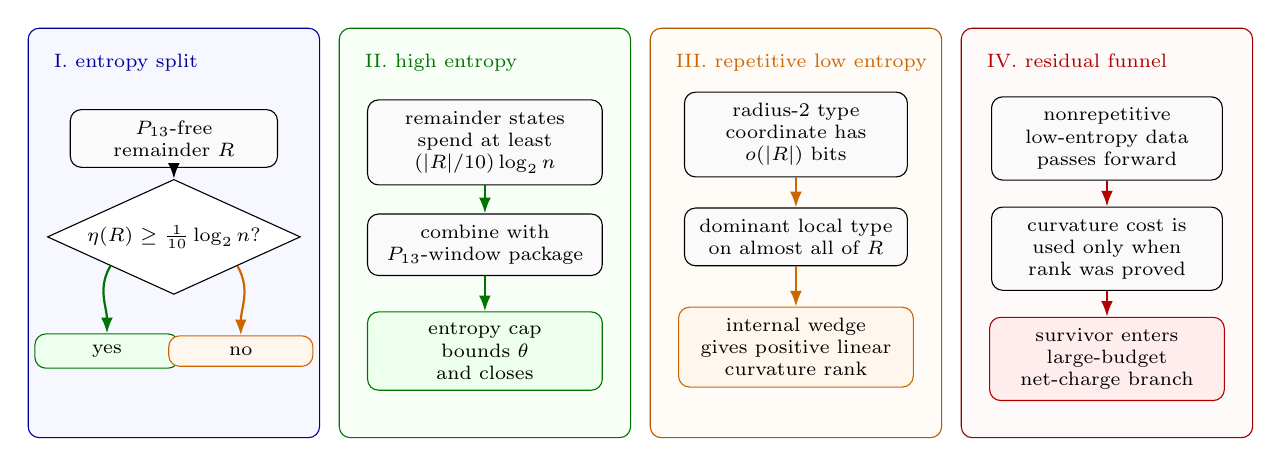
\begin{tikzpicture}[
box/.style={rectangle,rounded corners,draw,fill=black!2,align=center,inner sep=4pt,text width=2.55cm},
good/.style={rectangle,rounded corners,draw=green!45!black,fill=green!7,align=center,inner sep=4pt,text width=2.55cm},
warn/.style={rectangle,rounded corners,draw=orange!80!black,fill=orange!7,align=center,inner sep=4pt,text width=2.55cm},
bad/.style={rectangle,rounded corners,draw=red!70!black,fill=red!7,align=center,inner sep=4pt,text width=2.55cm},
test/.style={diamond,aspect=2.2,draw,fill=white,align=center,inner sep=1.2pt,text width=2.30cm},
arr/.style={-{Latex[length=2mm]},thick},
dasharr/.style={-{Latex[length=2mm]},thick,dashed},
every node/.style={font=\scriptsize}
]
\draw[rounded corners,fill=blue!3,draw=blue!60!black] (-7.75,-2.65) rectangle (-4.05,2.55);
\draw[rounded corners,fill=green!3,draw=green!45!black] (-3.80,-2.65) rectangle (-0.10,2.55);
\draw[rounded corners,fill=orange!3,draw=orange!70!black] (0.15,-2.65) rectangle (3.85,2.55);
\draw[rounded corners,fill=red!2,draw=red!60!black] (4.10,-2.65) rectangle (7.80,2.55);
\node[anchor=north west,blue!60!black] at (-7.55,2.35) {I. entropy split};
\node[anchor=north west,green!45!black] at (-3.60,2.35) {II. high entropy};
\node[anchor=north west,orange!80!black] at (0.35,2.35) {III. repetitive low entropy};
\node[anchor=north west,red!70!black] at (4.30,2.35) {IV. residual funnel};

\node[box,text width=2.35cm] (rem) at (-5.90,1.15) {\(P_{13}\)-free\\remainder \(R\)};
\node[test] (eta) at (-5.90,-0.10) {\(\eta(R)\ge\frac1{10}\log_2 n\)?};
\node[good,text width=1.55cm] (high) at (-6.75,-1.55) {yes};
\node[warn,text width=1.55cm] (low) at (-5.05,-1.55) {no};
\draw[arr] (rem)--(eta);
\draw[arr,green!45!black] (eta.south west) to[out=-120,in=90] (high.north);
\draw[arr,orange!80!black] (eta.south east) to[out=-60,in=90] (low.north);

\node[box,text width=2.70cm] (bits) at (-1.95,1.10) {remainder states\\spend at least\\\((|R|/10)\log_2 n\)};
\node[box,text width=2.70cm] (pack) at (-1.95,-0.20) {combine with\\\(P_{13}\)-window package};
\node[good,text width=2.70cm] (cap) at (-1.95,-1.55) {entropy cap\\bounds \(\theta\)\\and closes};
\draw[arr,green!45!black] (bits)--(pack);
\draw[arr,green!45!black] (pack)--(cap);

\node[box,text width=2.55cm] (typebits) at (2.00,1.20) {radius-\(2\) type\\coordinate has\\\(o(|R|)\) bits};
\node[box,text width=2.55cm] (dom) at (2.00,-0.10) {dominant local type\\on almost all of \(R\)};
\node[warn,text width=2.70cm] (rank) at (2.00,-1.50) {internal wedge\\gives positive linear\\curvature rank};
\draw[arr,orange!80!black] (typebits)--(dom);
\draw[arr,orange!80!black] (dom)--(rank);

\node[box,text width=2.65cm] (nonrep) at (5.95,1.15) {nonrepetitive\\low-entropy data\\passes forward};
\node[box,text width=2.65cm] (cost) at (5.95,-0.25) {curvature cost is\\used only when\\rank was proved};
\node[bad,text width=2.70cm] (large) at (5.95,-1.65) {survivor enters\\large-budget\\net-charge branch};
\draw[arr,red!70!black] (nonrep)--(cost);
\draw[arr,red!70!black] (cost)--(large);
\end{tikzpicture}%
}
\caption[Visual proof of the two-budget routing funnel]{Visual proof of the two-budget routing funnel.  Panel I splits the \(P_{13}\)-free remainder by its per-vertex skeleton entropy \(\eta(R)\).  Panel II shows the high-entropy branch: \(\eta(R)\ge\frac1{10}\log_2 n\) spends \((|R|/10)\log_2 n\) bits, and together with the independent \(P_{13}\)-window package gives the packing bound used by the entropy cap.  Panel III shows the structurally repetitive low-entropy branch: subexponential radius-\(2\) type data gives a dominant local type, and an internal length-two wedge in that type supplies positive linear curvature rank.  Panel IV records the routing convention of \cref{prop:two-budget}: nonrepetitive low-entropy data is passed to the large-budget net-charge branch, and curvature cost is carried forward only on branches where the preceding rank-forcing lemmas have established it.}
\label{fig:two-budget-routing-funnel}
\end{figure}

\begin{remark}[Role of the forced curvature cost]\label[remark]{rem:forced-cost-role}
When \cref{lem:full-rank} is invoked, the window-only forced curvature cost is
$K_{\rm win}|R|-o(|R|)$.  In the sharper high-entropy low-deficiency branch this
improves to $K|R|-o(|R|)$, and that sharper value is the numerical constraint
used in the entropy cap of \cref{prop:entropy-high-theta}.  The weaker
separated-translate input of \cref{lem:translates-independent} supplies only a
positive linear rank in the structurally repetitive low-entropy branch.  The
final large-budget closure outside the explicit residuals does not require the
exact curvature constant: \cref{rem:closure-robust} records that the
window-density and net-charge accounting already give the needed normalized
deficiency gap.
\end{remark}

\paragraph{Framework branch table.}
The two-budget routing funnel is summarized by the following framework table.
\begin{longtable}{L{0.13\textwidth} L{0.19\textwidth} L{0.14\textwidth} L{0.14\textwidth} L{0.17\textwidth} L{0.17\textwidth}}
\FrameworkBranchTableHeader
High entropy
&
\(\eta(R)\ge\frac1{10}\log_2 n\).
&
Remainder bits.
&
Skeleton entropy.
&
One target-coordinate family.
&
\cref{prop:two-budget,prop:p13-density}.
\\
\addlinespace
Repetitive low entropy
&
A radius-\(2\) coordinate has \(o(|R|)\) bits.
&
A dominant local type.
&
Separated curvature translates.
&
Bounded-radius overlap.
&
\cref{lem:dominant-type,lem:translates-independent}.
\\
\addlinespace
Nonrepetitive low entropy
&
The low-entropy data do not give dominance.
&
No local entropy closure here.
&
The large-budget route.
&
Not applicable.
&
Passed to \cref{sec:large-budget}.
\\
\addlinespace
Cost separation
&
Curvature cost is available only after rank forcing.
&
Independent tests.
&
The entropy budget.
&
The rank-forced branch.
&
\cref{rem:forced-cost-role}.
\\
\bottomrule
\end{longtable}

\section{The admissible entropy cap}

In this section assume \cref{def:near-cubic-spine}.  The entropy cap is
admissible only when the remaining non-curvature budget is smaller than the
forced curvature cost.  We make this precise.  In the high-entropy accounting of
\cref{sec:entropy-bound}, the window and remainder contributions consume, per
factor $n\log_2 n$, the normalized amount
\[
0.1+116.808581006\,\theta
\]
of the near-cubic labelled skeleton budget
\[
1.5\,n\log_2 n+o(n\log n)
\]
of \cref{lem:near-cubic-budget}.  Hence the \emph{remaining non-curvature budget} is
\[
\bigl(1.5-(0.1+116.808581006\,\theta)\bigr)n\log_2 n=\bigl(1.4-116.808581006\,\theta\bigr)n\log_2 n .
\]
On top of this, \cref{cor:forced-curvature-cost} imposes the linear forced curvature cost
\[
K|R|-o(|R|)=K(1-13\theta)n-o(n),\qquad K=5.89262883286\ldots .
\]
For a residual graph to exist, the window, remainder, and forced-curvature demands together must fit inside the skeleton budget; equivalently the forced curvature cost must fit inside the remaining non-curvature budget,
\[
K(1-13\theta)n\le\bigl(1.4-116.808581006\,\theta\bigr)n\log_2 n+o(n\log n).
\]
Dividing by $n$, no residual graph exists once
\begin{equation}\label{eq:entropy-cap}
\left(1.4-116.808581006\,\theta\right)\log_2 n
< K(1-13\theta).
\end{equation}

\begin{definition}[The finite-size packing threshold]\label[definition]{def:Theta}
Define
\[
\Theta(n)=
\frac{
1.4-\dfrac{K}{\log_2 n}
}{
116.808581006-\dfrac{13K}{\log_2 n}
},
\]
where
\[
K=5.89262883286\ldots .
\]
\end{definition}

\begin{proposition}[Entropy cap closes the high-$\theta$ branch]\label[proposition]{prop:entropy-high-theta}
Assume \cref{def:near-cubic-spine}.
In the high-entropy branch of \cref{prop:two-budget}, if
\[
\theta>\Theta(n)+o(1),
\]
then no minimal residual graph exists.
\end{proposition}

\begin{proof}
Suppose $\theta>\Theta(n)+o(1)$.  By the definition of $\Theta(n)$ this is precisely inequality~\eqref{eq:entropy-cap}, that is, the remaining non-curvature budget is strictly smaller than the forced full-rank curvature cost of \cref{cor:forced-curvature-cost}.  Then the window package of \cref{lem:p13-window-package}, the remainder bits, and the forced-curvature bits together strictly exceed the near-cubic skeleton budget $1.5\,n\log_2 n+o(n\log n)$.  These bits form one independently target-testable coordinate family, so the number of realized target-complete states would exceed the number of labelled skeletons, contradicting \cref{lem:independent-target-entropy,lem:skeleton-dominates}.  Hence no residual graph exists in this branch.
\end{proof}

\begin{remark}[Order of the entropy argument]\label[remark]{rem:entropy-argument-order}
The entropy cap is not used to assert an a priori linear upper bound on $r_\Omega(R)$.  Instead, the rank-forcing argument first forces full curvature rank.  Entropy is then applied only in the region where the remaining budget is smaller than the forced curvature cost.
\end{remark}

\begin{remark}[Robustness of the closure to the forced curvature cost]\label[remark]{rem:closure-robust}
The forced curvature cost sharpens the high-entropy threshold $\Theta(n)$ of
\cref{def:Theta}, but the large-budget closure outside the explicit residuals
does not need that sharpening.  The near-cubic window-only part of
\cref{prop:p13-density} gives
\[
\theta\le\theta_{\rm win}+o(1),
\qquad
\theta_{\rm win}=0.01270017798\ldots,
\]
and therefore
\[
\frac{15\theta}{1-13\theta}
\le
\tau_{\rm win}+o(1),
\qquad
\tau_{\rm win}=0.22817486846\ldots<\frac14 .
\]
Thus the curvature-rank and forced-cost machinery is not required for the
net-charge closure outside the explicit residuals, which already follows from
the window-only density bound together with the local analysis of
\cref{sec:large-budget,sec:local-analysis}.  Consequently the final closure
uses neither the exact value of $c_\Omega$ (\cref{rem:curvature-provenance}) nor
the precise rank fraction (\cref{rem:positive-fraction}) as an additional
hypothesis.
\end{remark}

\begin{center}
\begin{tabular}{rrrr}
\toprule
$n$ & $\log_2 n$ & $\Theta(n)$ & $\tau_{\Theta}=15\Theta(n)/(1-13\Theta(n))$\\
\midrule
$10^3$ & $9.9658$ & $0.007411$ & $0.123019$\\
$10^4$ & $13.2877$ & $0.008614$ & $0.145505$\\
$10^6$ & $19.9316$ & $0.009776$ & $0.167991$\\
$10^9$ & $29.8974$ & $0.010529$ & $0.182982$\\
$10^{12}$ & $39.8631$ & $0.010899$ & $0.190477$\\
$\infty$ & $\infty$ & $0.011985$ & $0.212963$\\
\bottomrule
\end{tabular}
\end{center}

\paragraph{Framework branch table.}
The admissible entropy cap closes only the branch where its numerical
inequality is active.
\begin{longtable}{L{0.13\textwidth} L{0.19\textwidth} L{0.14\textwidth} L{0.14\textwidth} L{0.17\textwidth} L{0.17\textwidth}}
\FrameworkBranchTableHeader
Admissible cap
&
The remaining non-curvature budget is smaller than the forced curvature cost.
&
Window, remainder, and curvature bits.
&
The near-cubic skeleton budget.
&
One target-complete coordinate family.
&
Closed by \cref{prop:entropy-high-theta}.
\\
\addlinespace
Below threshold
&
The entropy inequality does not close.
&
The large-budget residual.
&
Net-charge accounting.
&
Not applicable.
&
Routed to \cref{sec:large-budget}.
\\
\addlinespace
Robust route
&
The exact curvature magnitude is not used.
&
Window-only deficiency gap.
&
Net-charge and local discharging.
&
The same residual ledger.
&
\cref{rem:closure-robust}.
\\
\bottomrule
\end{longtable}

\section{The large-budget residual}\label{sec:large-budget}

Throughout this section assume \cref{def:near-cubic-spine}.
Regardless of whether the high-entropy cap of
\cref{prop:entropy-high-theta} applies, the near-cubic window-only bound in
\cref{prop:p13-density} gives
\[
\theta\le\theta_{\rm win}+o(1),
\qquad
|R|=n-13p=(1-13\theta)n\ge(1-13\theta_{\rm win})n-o(n).
\]
By maximality of the induced-$P_{13}$ packing, every component of $R$ is $P_{13}$-free.  By \cref{thm:p13free}, no component of $R$ has an internal subgraph of minimum degree at least $3$.

\begin{definition}[Internal \(3\)-core]\label[definition]{def:internal-3-core}
For a graph or support \(X\), the \emph{internal \(3\)-core} of \(X\) is the
maximal induced subgraph of \(X\) with minimum degree at least \(3\), obtained
equivalently by repeatedly deleting vertices of internal degree at most \(2\).
The internal \(3\)-core is \emph{empty} if no nonempty subgraph of \(X\) has
minimum internal degree at least \(3\).
\end{definition}

The supply inequality \cref{lem:stub-positive} gives
\[
\defp(R)-\sigma_R\le 15p_{13}+o(n),
\qquad \sigma_R=\sigma(R).
\]
Dividing by $|R|=(1-13\theta)n+o(n)$ yields
\[
\frac{\defp(R)-\sigma_R}{|R|}
\le
\frac{15\theta}{1-13\theta}+o(1).
\]
Since $\theta\le\theta_{\rm win}+o(1)$, every large-budget residual satisfies
\[
\boxed{
\frac{\defp(R)-\sigma_R}{|R|}
\le
\tau_{\rm win}+o(1),
}
\]
where
\[
\tau_{\rm win}=\frac{15\theta_{\rm win}}{1-13\theta_{\rm win}}
=0.22817486846\ldots<\frac14 .
\]

\begin{definition}[Canonical support decomposition]\label[definition]{def:canonical-decomp}
The \emph{canonical support decomposition} of the residual consists of:
\begin{enumerate}[label=(\roman*), leftmargin=2.2em]
\item the connected components $Y_1,\ldots,Y_k$ of $R$, ordered by the
deterministic tie-breaking rule fixed in \cref{lem:skeleton-dominates}; and
\item an assignment of every ambient surplus unit
$d_G(h)-3$ with $h\in V_{\ge4}(G)\cap V(R)$ to exactly one piece.
\end{enumerate}
All surplus units of $h\in V_{\ge4}(G)\cap V(R)$ are assigned to the unique
piece containing $h$.  Surplus carried by vertices in the packed windows is not
assigned to local supports; it has already been absorbed into the
$o(n)$ term in \cref{lem:stub-positive}.
For the support associated to $Y_i$, write
\[
|V(X_i)|:=|Y_i|,
\qquad
\sigma(X_i):=\text{the number of surplus units assigned to }Y_i .
\]
Thus
\[
\sum_i |V(X_i)|=|R|,
\qquad
\sum_i\sigma(X_i)=\sigma(R).
\]
When an assigned surplus unit is represented by an actual high-degree fan
vertex in the local Type B analysis, the corresponding fan envelope records
that vertex as decoration data; it is not counted a second time in
$|V(X_i)|$.  Because the pieces are the connected components of \(R\), there
are no edges of \(R\) between distinct pieces.
\end{definition}

\begin{definition}[Admissible support]\label[definition]{def:admissible}
An \emph{admissible support} $X$ is a connected remainder piece $Y_i$ of the
canonical support decomposition, together with its assigned surplus units and
any local decoration data needed to realize those units in the Type B fan
analysis.  Its vertex count and positive deficiency are those of the remainder
piece:
\[
|V(X)|=|Y_i|,
\qquad
\defp(X)=\sum_{v\in Y_i}\max\{0,3-d_{Y_i}(v)\}.
\]
Its surplus $\sigma(X)$ is the assigned surplus credit from
\cref{def:canonical-decomp}.  As a boundaried support of the minimal
counterexample $G$, $X$ carries the inherited constraints used in the local
analysis: it is $P_{13}$-free, has empty internal $3$-core, is dyadic-safe in
the contextual sense
(\cref{def:dyadic-safe}), has its deficient vertices supplied from the packing
$W$ (\cref{lem:stub-positive}), and is hereditarily target-uncompressible
(\cref{cor:uncompressible}).  The quantities $\defp(X)$, $\sigma(X)$, and
$\No(X)$ below are therefore accounting data for the embedded support, not
invariants of an isolated graph.
\end{definition}

\begin{definition}[Net charge]\label[definition]{def:net-charge}
For an admissible support $X$, define
\[
\No(X)=\defp(X)-\sigma(X)-\frac14|V(X)|.
\]
\end{definition}

\begin{figure}[t]
\centering
\resizebox{0.96\textwidth}{!}{%
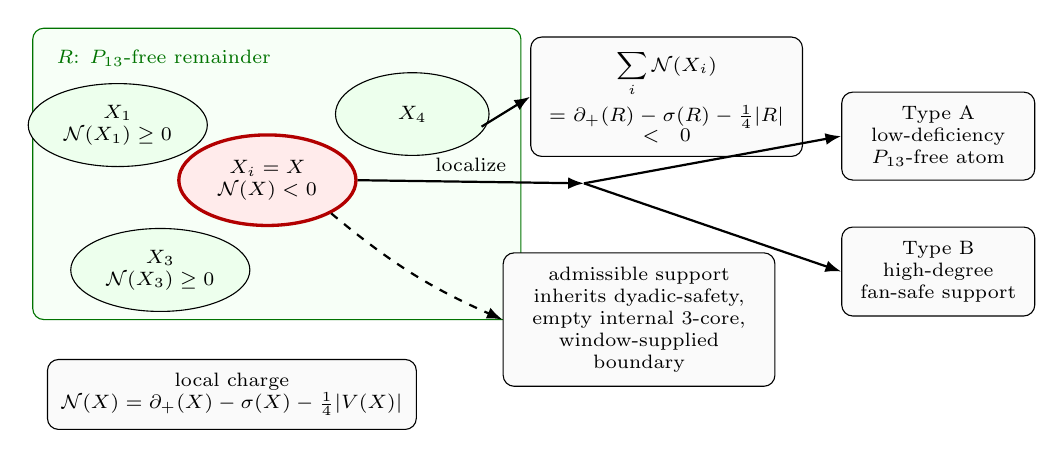
\begin{tikzpicture}[
support/.style={ellipse,draw,fill=green!7,minimum width=1.95cm,minimum height=1.05cm,align=center},
neg/.style={ellipse,draw=red!70!black,very thick,fill=red!8,minimum width=2.25cm,minimum height=1.15cm,align=center},
branch/.style={rectangle,rounded corners,draw,align=center,inner sep=5pt,fill=black!2},
widebranch/.style={rectangle,rounded corners,draw,align=center,inner sep=5pt,fill=black!2,text width=3.10cm},
typebranch/.style={rectangle,rounded corners,draw,align=center,inner sep=5pt,fill=black!2,text width=2.10cm},
arr/.style={-{Latex[length=2mm]},thick},
every node/.style={font=\scriptsize}
]
\draw[rounded corners,fill=green!3,draw=green!45!black] (-4.80,-1.55) rectangle (1.40,2.15);
\node[anchor=north west,green!45!black] at (-4.62,2.00) {$R$: $P_{13}$-free remainder};
\node[support] (x1) at (-3.72,0.92) {$X_1$\\$\No(X_1)\ge0$};
\node[neg] (x2) at (-1.82,0.22) {$X_i=X$\\$\No(X)<0$};
\node[support] (x3) at (-3.18,-0.92) {$X_3$\\$\No(X_3)\ge0$};
\node[support] (x4) at (0.02,1.06) {$X_4$};
\node[widebranch] (sum) at (3.25,1.28) {$\displaystyle\sum_i\No(X_i)$\\[2pt]
$=\defp(R)-\sigma(R)-\frac14|R|$\\[-1pt]
$<0$};
\draw[arr] (0.90,0.90)--(sum.west);
\coordinate (split) at (2.20,0.18);
\draw[arr] (x2.east)--node[above] {localize} (split);
\node[typebranch] (typeA) at (6.70,0.78) {Type A\\low-deficiency\\$P_{13}$-free atom};
\node[typebranch] (typeB) at (6.70,-0.94) {Type B\\high-degree\\fan-safe support};
\node[widebranch] (inherit) at (2.90,-1.55) {admissible support\\inherits dyadic-safety,\\empty internal $3$-core,\\window-supplied boundary};
\draw[arr] (split)--(typeA.west);
\draw[arr] (split)--(typeB.west);
\draw[arr,dashed] (x2.south east) to[bend right=8] (inherit.west);
\node[branch,anchor=north west] at (-4.62,-2.05) {local charge\\
$\No(X)=\defp(X)-\sigma(X)-\frac14|V(X)|$};
\end{tikzpicture}%
}
\caption[Visual definition of net-charge localization]{Visual definition of net-charge localization.  The green rectangle is the $P_{13}$-free remainder $R$, decomposed into connected admissible supports $X_i$ by the canonical support decomposition.  Green ellipses show supports with nonnegative net charge; the red ellipse is the localized support $X=X_i$ with $\No(X)<0$.  Each support carries positive deficiency $\defp(X_i)$, assigned ambient surplus $\sigma(X_i)$, and net charge $\No(X_i)=\defp(X_i)-\sigma(X_i)-\frac14|V(X_i)|$.  The top budget box records additivity over connected components, $\sum_i\No(X_i)=\defp(R)-\sigma(R)-\frac14|R|<0$.  The solid arrow labelled ``localize'' selects a negative support, the dashed arrow records inherited admissibility data, and the two outgoing solid arrows route that support to the Type A low-deficiency atom branch or the Type B high-degree fan-safe support branch.  The inherited data are contextual dyadic-safety, empty internal $3$-core, componentwise $P_{13}$-freeness, and window-supplied deficient boundary.}
\label{fig:netcharge-localization-gadget}
\end{figure}


\begin{lemma}[Net-charge localization under support splitting]\label[lemma]{lem:netcharge-superadd}
Let $R$ be decomposed canonically into connected admissible supports
$X_1,\ldots,X_k$.  Then
\[
\sum_{i=1}^{k}\No(X_i)
\ =
\defp(R)-\sigma(R)-\frac14|R|.
\]
Consequently, if
\[
\defp(R)-\sigma(R)-\frac14|R|< -\varepsilon |R|
\]
for some fixed $\varepsilon>0$, then some connected support $X_i$ has
$\No(X_i)<0$.
\end{lemma}

\begin{proof}
The remainder vertex sets $Y_i$ form a partition of $V(R)$, and the ambient
surplus units form a disjoint assigned credit partition.  By
\cref{def:canonical-decomp},
\[
\sum_i|V(X_i)|=|R|,
\qquad
\sum_i\sigma(X_i)=\sigma(R).
\]

For each vertex $u\in Y_i$, the component property gives
$d_{X_i}(u)=d_R(u)$.  Hence the positive deficiencies add exactly:
\[
\sum_i\defp(X_i)=\defp(R).
\]
Therefore
\[
\sum_i\No(X_i)=\sum_i\defp(X_i)-\sigma(R)-\frac14|R|
=\defp(R)-\sigma(R)-\frac14|R|,
\]
the displayed identity.  If the right-hand side is negative by a
linear amount and all summands were nonnegative, their sum could not be negative;
hence some connected support has negative net charge.
\end{proof}

\begin{corollary}[Global window-join pressure]\label[corollary]{cor:global-window-join-pressure}
Let \(R\) be decomposed canonically into connected admissible supports
\(X_1,\ldots,X_k\).  Then
\[
\sum_{i=1}^k \No(X_i)
\le
15p_{13}+\sigma_W-\sigma_R-\frac14|R|.
\]
Consequently, if every connected admissible support in this decomposition has
nonnegative net charge, then
\[
\sigma_W-\sigma_R
\ge
\frac14|R|-15p_{13}
=\frac{n-73p_{13}}4 .
\]
Equivalently, if \(p_{13}\le \theta n+o(n)\), then the no-negative-support
alternative forces
\[
\sigma_W-\sigma_R
\ge
\frac{1-73\theta}{4}\,n-o(n).
\]
In particular, under the near-cubic window-only cap
\(\theta\le\theta_{\rm win}+o(1)\),
\[
\sigma_W-\sigma_R
\ge
\kappa_{\rm win}n-o(n),
\qquad
\kappa_{\rm win}:=\frac{1-73\theta_{\rm win}}4
=0.0182217518254\ldots .
\]
\end{corollary}

\begin{proof}
By \cref{lem:netcharge-superadd},
\[
\sum_i\No(X_i)
=\defp(R)-\sigma_R-\frac14|R|.
\]
The surplus-aware window-stub inequality
\cref{lem:surplus-aware-window-stub} gives
\[
\defp(R)-\sigma_R
\le
15p_{13}+\sigma_W-\sigma_R.
\]
Combining the two displays proves the first inequality.

If every \(X_i\) has \(\No(X_i)\ge0\), then the left-hand side is nonnegative.
Therefore
\[
0\le15p_{13}+\sigma_W-\sigma_R-\frac14|R|,
\]
which is the displayed lower bound on \(\sigma_W-\sigma_R\).  Since
\(|R|=n-13p_{13}\), this lower bound equals
\[
\frac{n-13p_{13}}4-15p_{13}
=\frac{n-73p_{13}}4.
\]
The density forms follow by substituting \(p_{13}\le\theta n+o(n)\) and then
\(\theta=\theta_{\rm win}+o(1)\).
\end{proof}

\begin{remark}[Meaning of the join-pressure inequality]\label[remark]{rem:window-join-pressure-meaning}
\Cref{cor:global-window-join-pressure} is the exact accounting form of the
non-near-cubic pressure.  Surplus carried by \(R\) appears with a negative sign
in \(\No(R)\), so it helps produce a negative admissible support.  Avoiding such
a support requires a linear excess of window surplus over remainder surplus.
By \cref{lem:exact-window-join-identity}, that excess is not abstract: it is
realized by additional window--remainder incidences and cross-window joins.
\end{remark}

\begin{proposition}[Large-budget residual is negative-net-charge]\label[proposition]{prop:negative-net-charge}
If the large-budget branch survives and the local lower bound fails by a fixed
linear margin, i.e. if for some $\varepsilon>0$,
\[
\defp(R)-\sigma(R)\le\frac14|R|-\varepsilon|R|
\]
for all sufficiently large $n$, then there is a connected admissible support
$X$ with
\[
\No(X)<0.
\]
\end{proposition}


\begin{proof}
By \cref{lem:netcharge-superadd},
\[
\sum_i\No(X_i)=\defp(R)-\sigma(R)-\frac14|R|.
\]
By the displayed hypothesis, the right-hand side is negative for all
sufficiently large $n$.  Hence at least one connected admissible support $X_i$
has negative net charge.  Choose such a support and call it $X$.
\end{proof}

\paragraph{Framework branch table.}
The large-budget residual localizes negative mass by the following branch
table.
\begin{longtable}{L{0.13\textwidth} L{0.19\textwidth} L{0.14\textwidth} L{0.14\textwidth} L{0.17\textwidth} L{0.17\textwidth}}
\FrameworkBranchTableHeader
Net-charge cap
&
\(\defp(R)-\sigma(R)<\frac14|R|\).
&
Negative total charge.
&
The support decomposition.
&
The superadditive component sum.
&
\cref{lem:netcharge-superadd}.
\\
\addlinespace
Localization
&
The total net charge is negative.
&
A connected deficit support.
&
The admissible support class.
&
The component partition.
&
\cref{prop:negative-net-charge}.
\\
\addlinespace
Window pressure
&
No negative support appears without surplus pressure.
&
\(\sigma_W-\sigma_R\).
&
The window-join identity.
&
The stub partition.
&
\cref{cor:global-window-join-pressure}.
\\
\bottomrule
\end{longtable}

\section{Local analysis of a negative-net-charge support}\label{sec:local-analysis}

Let $X$ be a connected admissible support with
\[
\No(X)<0.
\]
We show that $X$ is forced into one of two local obstruction classes.

\begin{remark}[How to read the local lemmas]\label[remark]{rem:local-reading}
The support $X$ is \emph{admissible} (\cref{def:admissible}): a piece of the minimal counterexample $G$, so it carries every global constraint, not merely its own induced structure.  In particular it is dyadic-safe in the strong, contextual sense (\cref{def:dyadic-safe})---$G$ has no power-of-two cycle meeting $V(X)$, including cycles that leave $X$ through its boundary and return through $G-X$---its deficient vertices are supplied from the packing $W$ (\cref{lem:stub-positive}), and it is hereditarily target-uncompressible (\cref{cor:uncompressible}).  Consequently the inequalities $\No(X)\ge0$ proved below are \emph{not} intrinsic properties of subcubic, empty-$3$-core, $P_{13}$-free graphs taken in isolation---such graphs may violate them---but properties of supports that admit a completion to a graph of minimum degree three with no power-of-two cycle.  Every step uses this admissibility; a lemma read with only its bare graph hypotheses has been read with strictly fewer hypotheses than it states.
\end{remark}

\subsection{Type A: low-deficiency \texorpdfstring{$P_{13}$}{P13}-free atom}

If $X$ carries no high-degree surplus, then $\sigma(X)=0$ and
\[
\No(X)<0
\]
means
\[
\defp(X)<\frac14|V(X)|.
\]
If $X$ is subcubic, then $\defp(X)=\sum_{v\in V(X)}(3-d_X(v))=3|V(X)|-2|E(X)|$, so $\defp(X)<\tfrac14|V(X)|$ is equivalent to $3|V(X)|-2|E(X)|<\tfrac14|V(X)|$, that is
\[
\frac{2|E(X)|}{|V(X)|}>2.75.
\]
Since $X$ lies in the $P_{13}$-free remainder, it is $P_{13}$-free.  We first bound its diameter.  A shortest path between two vertices is always induced, so if $X$ had two vertices at distance $12$, the shortest path between them would be an induced path on $13$ vertices, i.e.\ an induced $P_{13}$, contradicting $P_{13}$-freeness.  Hence $\diam(X)\le11$.  Consequently breadth-first layering from any root $v_0$ has at most $\diam(X)+1=12$ layers; since $X$ is subcubic, the first layer (the neighbours of $v_0$) has at most $3$ vertices, and each vertex in a later layer contributes at most $2$ vertices to the next layer, one of its at most three incident edges leading back toward the root.  Therefore
\[
|V(X)|\le 1+3\sum_{i=0}^{10}2^i=1+3(2^{11}-1)=6142.
\]
If the root has degree at most $2$, this improves to $1+2(2^{11}-1)=4095$; in either case the Type A class is finite:
\[
|V(X)|\le6142,
\qquad
\defp(X)<|X|/4,
\qquad
X\text{ is }P_{13}\text{-free and dyadic-safe.}
\]

The exclusion of this class is established by a contextual density lemma.  The
lemma is stated separately because the bound is a statement about completions in
$G$, not about isolated $P_{13}$-free graphs.

\begin{definition}[Type A support]\label[definition]{def:typeA-support}
A \emph{Type A support} is a connected admissible support $X$ with
$\sigma(X)=0$.  Since $G$ has minimum degree at least $3$, this condition gives
$d_G(v)=3$ for every $v\in V(X)$.  Hence $X$ is subcubic, the deficient vertices
of $X$ are exactly the vertices of internal degree at most $2$, and the
$P_{13}$-freeness, empty internal $3$-core, contextual dyadic-safety, supplied
deficiency, and hereditary target-uncompressibility of $X$ are inherited from
\cref{def:admissible}.  In the negative-net-charge branch a Type A support also
satisfies $\defp(X)<|V(X)|/4$.
\end{definition}

\begin{definition}[Receivers, ports, and routed load]\label[definition]{def:typeA-receiver-load}
Let $X$ be a Type A support.  A \emph{receiver} is a vertex
$w\in V(X)$ with $d_X(w)\le2$, and
\[
q(w)=3-d_X(w).
\]
Since $\sigma(X)=0$, every vertex of $X$ has ambient degree exactly $3$, so
$q(w)$ is also the number of ambient edges from $w$ to $G-X$.  An oriented edge
$\vec e=(w,h)$ with $wh\in E(G)\setminus E(X)$ is a \emph{completion port} of
$w$.

Let $X_3$ be the subgraph induced by the vertices of $X$ with internal degree
$3$.  The empty internal $3$-core condition implies that every component of
$X_3$ has an edge to at least one receiver.  For a cubic vertex $u$, let
$T_u$ be the lexicographically first path in $X$ that starts at $u$, stays in
$X_3$ until its last edge, and ends at a receiver; write this terminal receiver
as $r(u)$.  The path $T_u$ is the \emph{canonical trace} of $u$.  The routed load
at $w$ is
\[
L(w)=|\{u\in V(X):d_X(u)=3,\ r(u)=w\}|.
\]
A receiver is \emph{saturated} when $L(w)\ge4q(w)$ and \emph{unsaturated}
when $L(w)\le4q(w)-1$.
For $j=0,1,2$, let
\[
\mathcal R_j(X)=\{w\in V(X):d_X(w)=2-j\}.
\]
\end{definition}

\begin{lemma}[Canonical receiver loads]\label[lemma]{lem:typeA-receiver-loads}
For every Type A support $X$, the map $u\mapsto r(u)$ is defined for each
degree-$3$ vertex of $X$, and every degree-$3$ vertex is assigned to exactly one
receiver.
\end{lemma}

\begin{proof}
The empty internal $3$-core hypothesis implies that no component of the induced
subgraph $X_3$ is closed under all three incident edges of its vertices.
Therefore each component of $X_3$ has an edge to a vertex of internal degree at
most $2$, i.e. to a receiver.  The canonical trace $T_u$ is chosen by a fixed
lexicographic tie-breaking rule among these receiver-reaching paths, so its
terminal receiver $r(u)$ is defined and unique.  Thus every degree-$3$ vertex is
assigned to exactly one receiver.
\end{proof}

\begin{definition}[Receiver-entry returns and visible load]\label[definition]{def:typeA-visible-load}
Let $\vec e=(w,h)$ be a completion port.  An \emph{anchored return} through
$\vec e$ is a simple path $P:h\leadsto w$ in $G-wh$.  Its first vertex in
$X$, traversed from $h$ to $w$, is denoted $\operatorname{ent}_X(P)$.

If $r,w$ are receivers, a \emph{receiver-entry channel} from $r$ to $w$ is a
simple path $Q:r\leadsto w$ in $X$.  An anchored return is a
\emph{receiver-entry return} if it decomposes as
\[
P=\Gamma\circ Q,
\]
where $\Gamma$ runs from $h$ to a receiver $r$ with internal vertices outside
$X$, and $Q$ is a receiver-entry channel from $r$ to $w$.

A receiver-entry return $P=\Gamma\circ Q$ through $\vec e$ is \emph{visible for}
a routed cubic vertex $u$ with $r(u)=w$ if the canonical trace $T_u$ is a
subpath of the channel $Q$, or if $Q$ is the lexicographically first channel
assigned to the terminal receiver edge of $T_u$.  The port $\vec e$ carries
$t$ visible receiver-entry returns when it carries such returns for $t$ distinct
routed cubic vertices.  Let $L_{\mathrm{vis}}(w,\vec e)$ be this number.  A load
routed to $w$ is \emph{visible} if it is visible at some completion port of $w$;
if more than one port sees it, it is assigned to the first such port in the
canonical order.  The total number of visible loads routed to $w$ is
$L_{\mathrm{vis}}(w)$; the remaining loads are \emph{silent} and have count
\[
L_{\mathrm{sil}}(w)=L(w)-L_{\mathrm{vis}}(w).
\]
\end{definition}

\begin{figure}[t]
\centering
\resizebox{0.98\textwidth}{!}{%
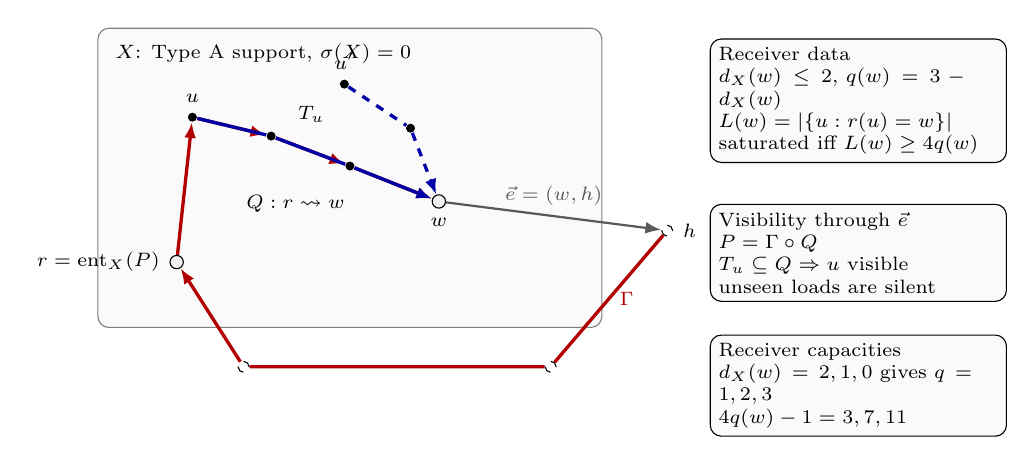
\begin{tikzpicture}[
vtx/.style={circle,fill=black,inner sep=1.15pt},
recv/.style={circle,draw,fill=black!5,inner sep=1.7pt},
outv/.style={circle,draw,dashed,inner sep=1.4pt},
trace/.style={-{Latex[length=2mm]},very thick,blue!65!black},
ret/.style={-{Latex[length=2mm]},very thick,red!70!black},
port/.style={-{Latex[length=2mm]},thick,black!65},
note/.style={rectangle,rounded corners,draw,align=left,inner sep=3pt,fill=black!2,text width=3.55cm},
every node/.style={font=\scriptsize}
]
\draw[rounded corners,fill=black!2,draw=black!50] (-4.05,-1.75) rectangle (2.35,2.05);
\node[anchor=north west] at (-3.95,1.98) {$X$: Type A support, $\sigma(X)=0$};

\node[vtx,label=above:$u$] (u) at (-2.85,0.92) {};
\node[vtx] (a) at (-1.85,0.68) {};
\node[vtx] (b) at (-0.85,0.30) {};
\node[recv,label=below:$w$] (w) at (0.28,-0.15) {};
\node[recv,label={left:$r=\operatorname{ent}_X(P)$}] (r) at (-3.05,-0.92) {};
\node[vtx,label=above:$u'$] (us) at (-0.92,1.34) {};
\node[vtx] (s) at (-0.08,0.78) {};

\draw[ret] (r)--(u);
\draw[ret] (u)--(a);
\draw[ret] (a)--(b);
\draw[ret] (b)--(w);
\draw[trace] (u)--(a)--(b)--(w);
\draw[trace,dashed] (us)--(s)--(w);

\node[outv,label=right:$h$] (h) at (3.18,-0.52) {};
\node[outv] (z1) at (1.70,-2.25) {};
\node[outv] (z2) at (-2.20,-2.25) {};
\draw[port] (w)--node[above]{$\vec e=(w,h)$} (h);
\draw[ret] (h)--node[right]{$\Gamma$} (z1)--(z2)--(r);
\node at (-1.34,0.96) {$T_u$};
\node at (-1.54,-0.18) {$Q:r\leadsto w$};

\node[note,anchor=north west] at (3.72,1.92) {Receiver data\\
$d_X(w)\le2$, $q(w)=3-d_X(w)$\\
$L(w)=|\{u:r(u)=w\}|$\\
saturated iff $L(w)\ge4q(w)$};
\node[note,anchor=north west] at (3.72,-0.18) {Visibility through $\vec e$\\
$P=\Gamma\circ Q$\\
$T_u\subseteq Q \Rightarrow u$ visible\\
unseen loads are silent};
\node[note,anchor=north west] at (3.72,-1.84) {Receiver capacities\\
$d_X(w)=2,1,0$ gives $q=1,2,3$\\
$4q(w)-1=3,7,11$};
\end{tikzpicture}%
}
\caption[Visual definition of a Type A receiver]{Visual definition of a Type A receiver.  The shaded region is the Type A support $X$, and $\sigma(X)=0$ records that the support has no ambient surplus.  White circled vertices are receivers; the terminal receiver is $w$, and $r=\operatorname{ent}_X(P)$ is the first vertex of $X$ met by the anchored return $P$.  Black filled vertices are internal vertices of the support or of a displayed trace.  The dashed circled vertex $h$ lies outside $X$, and the grey arrow $\vec e=(w,h)$ is the completion port being tested.  The red path is the anchored return $P=\Gamma\circ Q$: the outside connector $\Gamma$ runs from $h$ to $r$, while the internal receiver-entry channel $Q:r\leadsto w$ runs inside $X$.  The solid blue path $T_u$ is the canonical trace of the routed cubic vertex $u$ and makes $u$ visible at $\vec e$ because $T_u\subseteq Q$; the dashed blue trace from $u'$ illustrates a routed load not seen by this port.  The three legend boxes define the receiver data, visibility criterion, and receiver capacities.  Here $d_X(w)$ is the degree of $w$ inside $X$, $q(w)=3-d_X(w)$ is the number of missing ambient incidences at $w$, and $L(w)=|\{u:r(u)=w\}|$ is the number of routed cubic vertices assigned to $w$.  The receiver is saturated when $L(w)\ge4q(w)$, and the displayed capacities $3,7,11$ are the values of $4q(w)-1$ for $d_X(w)=2,1,0$.}
\label{fig:typeA-receiver-gadget}
\end{figure}

\begin{lemma}[Common-port return cycle]\label[lemma]{lem:typeA-common-port-return-cycle}
Let \(\vec e=(w,h)\) be a completion port, and let \(P_1,P_2\) be two anchored
returns through \(\vec e\).  If \(P_1\) and \(P_2\) are internally
vertex-disjoint as paths in \(G-wh\), then \(P_1\cup P_2\) is a simple cycle of
length \(|P_1|+|P_2|\).  In particular, if \(|P_1|+|P_2|\in\Pow\), then \(G\)
contains a dyadic cycle.
\end{lemma}

\begin{proof}
By definition, each anchored return through \(\vec e\) is a simple path from
\(h\) to \(w\) in \(G-wh\).  Thus the two paths have the same endpoints.  The
internal-disjointness hypothesis is exactly the hypothesis of
\cref{lem:two-path-criterion}, so their union is a simple cycle of the stated
length.
\end{proof}

\begin{lemma}[First entry is a receiver]\label[lemma]{lem:typeA-first-entry}
Let $P$ be an anchored return through a completion port of a Type A support
$X$.  Then $\operatorname{ent}_X(P)$ is a receiver.
\end{lemma}

\begin{proof}
Let $r=\operatorname{ent}_X(P)$.  The predecessor of $r$ on $P$ lies outside
$X$, so $r$ has an ambient incidence not counted in $d_X(r)$.  Since
$\sigma(X)=0$, every vertex of $X$ has ambient degree $3$.  Hence
$d_X(r)\le2$, and $r$ is a receiver.
\end{proof}

\begin{lemma}[Degree-two entry exclusion and entry budget]\label[lemma]{lem:typeA-entry-budget}
Let $w$ be a receiver with $d_X(w)=2$, and let $\vec e=(w,h)$ be its unique
completion port.  Every anchored return through $\vec e$ first enters $X$ at a
receiver $r\ne w$.  Moreover the number of distinct external edges through
which such returns first enter $X$ is at most
\[
\sum_{\substack{r\ \mathrm{receiver}\\ r\ne w}} q(r).
\]
\end{lemma}

\begin{proof}
An anchored return through $\vec e$ is a path from $h$ to $w$ in $G-wh$.  By
\cref{lem:typeA-first-entry}, its first vertex $r$ in $X$ is a receiver.  If
$r=w$, then the return enters $w$ from outside $X$ through an ambient edge
different from the deleted edge $wh$.  This is impossible because $d_X(w)=2$
and $\sigma(X)=0$ give exactly one ambient edge from $w$ to $G-X$, namely
$wh$.  Hence $r\ne w$.  For each first-entry receiver $r$, the entering edge is
one of the $q(r)$ completion ports of $r$, giving the displayed bound.
\end{proof}

\begin{lemma}[Ports have anchored returns]\label[lemma]{lem:typeA-port-return}
Every completion port of a Type A support has at least one anchored return.
\end{lemma}

\begin{proof}
A completion port is an oriented edge of $G$.  By \cref{lem:bridgeless}, the
underlying edge lies on a cycle in $G$.  Removing the port edge from that cycle
leaves a simple return path in the required orientation.
\end{proof}

\begin{definition}[Connector length and channel spectrum]\label[definition]{def:typeA-channel-spectrum}
Let $\vec e=(w,h)$ be a completion port and let
\[
P=\Gamma\circ Q
\]
be a receiver-entry return through $\vec e$, where $\Gamma$ runs from $h$ to
the first-entry receiver $r$ with internal vertices outside $X$, and
$Q:r\leadsto w$ lies in $X$.  The path $\Gamma$ is the \emph{connector}, and
its length is denoted $g(\Gamma)$.

For receivers $r,w$ define the \emph{internal channel spectrum}
\[
\Lambda_X(r,w)=\{|Q|:Q\text{ is a simple path in }X\text{ from }r\text{ to }w\}.
\]
The \emph{interval length} $I_X(r,w)$ is the largest cardinality of an interval
of consecutive integers contained in $\Lambda_X(r,w)$.
\end{definition}

\begin{definition}[Connector germs and continuation classes]\label[definition]{def:typeA-continuation-classes}
Let $X$ be a Type A support, let $\vec e=(w,h)$ be a completion port, and let
\[
P=\Gamma\circ Q
\]
be a receiver-entry return through $\vec e$.  Write
\[
\Gamma=(x_0,x_1,\ldots,x_g),
\qquad x_0=h,\qquad x_g=\operatorname{ent}_X(P),
\]
where $x_1,\ldots,x_{g-1}\notin X$.  The
\emph{outside connector germ} of $P$ is the ordered path $\Gamma$ together with
the first-entry receiver $x_g$, the channel $Q$, and the declared response
coordinate of \cref{def:declared-coordinate-signature} determined by
$(\vec e,x_g,g(\Gamma),Q)$.

Let $\kappa_i,\kappa_j$ be two declared response coordinates through the same
completion port, with connector germs $\Gamma_i,\Gamma_j$.  They have the same
\emph{continuation class up to an outside vertex $z$} when $z$ occurs in both
germs, the two germs have the same ordered prefix from $h$ to $z$, and the two
coordinates have the same image in the relevant boundary-degree fibre.  They
\emph{separate at $z$} when they have the same continuation class up to $z$ and
their next incidences after $z$ are distinct.  Here the next incidence may be an
edge from $z$ to an outside vertex or the first-entry edge from $z$ into $X$.

For a finite family $\mathcal K$ of declared response coordinates through
$\vec e$, a vertex $z\notin X$ is a \emph{first separator} of $\mathcal K$ if
some pair of coordinates in $\mathcal K$ separates at $z$ and no pair separates
at an earlier vertex on their common prefix from $h$.

If $\kappa_i,\kappa_j$ separate at $z$, the associated \emph{switch support}
$S_z(\kappa_i,\kappa_j)$ is the finite connected support consisting of the
common prefix from $h$ to $z$, the two connector tails from $z$ to their
first-entry receivers, the two receiver-entry channels in $X$, the completion
port boundary datum, and the declared supports of the two response coordinates.
The separator $z$ is \emph{absorbed} when the response identification on this
switch support is target-defective, target-complete on a nontrivial response
quotient, or target-complete only after adjoining a larger connected support.
It is \emph{surviving} when it is not absorbed.
\end{definition}

\begin{lemma}[Spectral interval pressure]\label[lemma]{lem:typeA-spectral-pressure}
Let $\vec e=(w,h)$ be a completion port and let $\Gamma$ be a connector from
$h$ to a first-entry receiver $r$.  Then
\[
g(\Gamma)+\lambda\notin\Mers
\qquad\text{for every }\lambda\in\Lambda_X(r,w).
\]
Consequently, if $\Lambda_X(r,w)$ contains the interval $[a,b]\cap\mathbb Z$,
then
\[
g(\Gamma)\notin
\bigcup_{\mu\in\Mers}\bigl([\mu-b,\mu-a]\cap\mathbb Z_{\ge1}\bigr).
\]
\end{lemma}

\begin{proof}
For any simple channel $Q:r\leadsto w$ in $X$, the concatenation
$\Gamma\circ Q$ is a simple return through $\vec e$: the internal vertices of
$\Gamma$ avoid $X$, while $Q$ lies in $X$.  If
$g(\Gamma)+|Q|\in\Mers$, then $\Gamma\circ Q$ together with the port edge gives
a power-of-two cycle by \cref{lem:return-equivalence}, contradicting the
counterexample condition.  Varying $Q$ over all channels gives the first
assertion.  The displayed band exclusion is the same statement applied to every
$\lambda\in[a,b]\cap\mathbb Z$.
\end{proof}

\begin{remark}[The receiver-5 witness and the band constraint]\label[remark]{rem:typeA-witness-pressure}
For the explicit $15$-vertex near-miss atom described in the referee material,
the receiver-channel spectra from the two other degree-$2$ receivers to the
saturated receiver are both the full interval $[3,14]$.  Thus a connector
length $g$ into either entry receiver must avoid
\[
\bigcup_{\mu\in\Mers}[\mu-14,\mu-3].
\]
In particular, below $112$ the allowed positive lengths are
\[
[13,16]\cup[29,48]\cup[61,112],
\]
and $[1,12]$ is forbidden.  This is not an additional external theorem; it is
the universally quantified target condition $R_e(G)\cap\Mers=\varnothing$
applied to all channel lengths at once.
\end{remark}

\begin{definition}[Silent trace basins]\label[definition]{def:typeA-trace-basin}
Let $u$ be a routed cubic vertex of a Type A support, and let $T_u$ be its
canonical trace ending at $r(u)$.  For a connected subgraph $S\subseteq X$
with $T_u\subseteq S$, let
\[
\partial S=\{v\in V(S): v\text{ is incident with an edge of }G-S\},
\]
and regard $S$ as a $\partial S$-boundaried graph with the inherited labels.
Each local target-response coordinate used in this paper has a declared finite
support: for example, a return coordinate is supported on its port and channel,
a $P_{13}$ label coordinate on its window, a curvature coordinate on its
length-two wedge, and a boundary-degree coordinate on the corresponding
boundary vertex.  A coordinate is \emph{$u$-supported} if its declared support
meets $T_u$, or if it is one of the completion-port labels, receiver-entry
channel lengths, connector-band constraints, boundary-degree entries, or
$P_{13}$ labels whose declared support in
\cref{def:declared-coordinate-signature} belongs to a receiver-entry return
whose internal channel contains $T_u$ or is canonically assigned to the terminal
receiver edge of $T_u$.  Let $\mathcal R_u(S)$ be the finite family of $u$-supported
coordinates carried by $S$.  The trace-incidence coordinate recording the
labelled path $T_u$ is included whenever $T_u\subseteq S$; hence a trace basin
always has at least one internal $u$-supported coordinate.

For $S\subseteq X$, let
\[
\operatorname{res}_{X,S}:\mathcal R_u(X)\dashrightarrow
\mathcal R_u(S)\cup\{\mathbf d_\partial(S)\text{-entries}\}
\]
be the partial restriction map which is defined on a coordinate precisely when
the coordinate's declared support is carried by $S$, or when its value is fixed
by the boundary degree profile $\mathbf d_\partial(S)$.  A connected
$S\subseteq X$ containing $T_u$ is \emph{trace-complete for $u$} if
$\operatorname{res}_{X,S}$ is defined on every coordinate of $\mathcal R_u(X)$
and the restricted value equals the value of that coordinate in $X$.  Since
$X$ itself is trace-complete for $u$, the finite set of trace-complete
connected subgraphs has lexicographically first inclusion-minimal elements.
The \emph{trace basin} $B_u$ is the lexicographically first such element.

The \emph{trace-response state} of $B_u$ is
\[
\rho_u(B_u)=
\bigl(\mathbf d_\partial(B_u),\mathcal R_u(B_u),\profile_{\partial B_u}(B_u)\bigr).
\]
The family $\mathcal R_u(B_u)$ is the complete declared coordinate family for
the $u$-supported target events used in the route-8 branch: once the boundary
degree profile and all entries of $\mathcal R_u(B_u)$ are fixed, every
compatible outside context has the same truth value for each such declared
event.  Carrier quotients below are tested only against this declared
$u$-supported target algebra.
A \emph{response quotient} of $\rho_u(B_u)$ is obtained by identifying or
forgetting entries of the finite coordinate family $\mathcal R_u(B_u)$ while
preserving the boundary degree profile.  A realization of such a quotient is a
boundaried response state with the same boundary degree profile whose image
under the quotient map is the given quotient.  The quotient is
\emph{target-complete} for $\rho_u(B_u)$ if, for every outside
$\partial B_u$-context compatible with the boundary profile, all realizations of
the quotient give the same target predicate as $\rho_u(B_u)$ after gluing.
Thus a target-complete quotient identifies only target-indistinguishable
response states.  The quotient is \emph{nontrivial} if it forgets or identifies
a coordinate whose declared support meets \(B_u-\partial B_u\), or whose
declared support contains an internal edge of \(B_u\), that is, an edge of
\(B_u\) with both endpoints in \(V(B_u)\).

A response quotient of \(\rho_u(B_u)\) is \emph{trace-local and non-carrier} if
it identifies or forgets entries of the fixed coordinate family
\(\mathcal R_u(B_u)\), preserves the full boundary degree profile, and does not
delete an ambient boundary carrier from the carrier set used later in
\cref{def:typeA-route8-carriers}.  Thus carrier-restriction and
carrier-deletion quotients are excluded from trace-complete-minimality; they
are tested only in the two-carrier clause of
\cref{def:typeA-exit4-family}.

The trace basin $B_u$ is \emph{target-complete-minimal} when none of the
following four alternatives occurs:
\begin{enumerate}[label=(\alph*), leftmargin=2.2em]
\item a trace-local non-carrier quotient or identification inside
\(\rho_u(B_u)\) is distinguished by some outside \(\partial B_u\)-context,
hence is target-defective;
\item $\rho_u(B_u)$ has a nontrivial target-complete response quotient with the
same boundary degree profile; when this quotient is realized by a smaller
connected representative, it is a target-complete compression of a proper atom;
\item an equality among coordinates of $\rho_u(B_u)$ becomes target-complete
only after adjoining a larger connected support $Z\supsetneq B_u$, either with
$Z\subsetneq G$ or with $Z=G$;
\item two declared outside connector germs of $\rho_u(B_u)$, with the same
boundary-degree image, have a surviving first separator in the sense of
\cref{def:typeA-continuation-classes}; by
\cref{lem:typeA-cubic-switch-absorption} this separator has ambient degree at
least $4$.
\end{enumerate}
Thus a trace basin that is not target-complete-minimal realizes, respectively,
one of the quotient, response-compression, delocalization, or decorated handoff
fan alternatives used below in exits (4)--(7).
\end{definition}

\begin{definition}[Silent-core residual profile]\label[definition]{def:typeA-silent-core-residual}
A \emph{silent-core residual profile} is the data
\[
(X,w,A(w),E(w),\mathcal U(w),(B_u)_{u\in\mathcal U(w)},
\{\Lambda_X(r,w)\}_r,\mathcal B)
\]
obtained from a saturated Type A receiver $w$ when no port carries four visible
receiver-entry returns and none of the target, quotient, compression,
delocalization, or decorated handoff fan alternatives applies.  Here $A(w)$ is the
canonical payable set of \cref{def:typeA-excess-basin}, $E(w)$ is the excess
basin, $\mathcal U(w)$ is the set of unpaid silent routed vertices in that
basin, $(B_u)_{u\in\mathcal U(w)}$ is the indexed family of trace basins from
\cref{def:typeA-trace-basin}, and $\mathcal B$ records the completion-port
labels and connector-length bands forced by
\cref{lem:typeA-port-return,lem:typeA-spectral-pressure}.  Such a profile is
\emph{admissible} only if every $B_u$ with
$u\in\mathcal U(w)$ is target-complete-minimal and all connector bands,
$P_{13}$ labels, boundary degree profiles, and cross-port theta constraints are
compatible with the standing counterexample invariants.
\end{definition}

\begin{definition}[Saturated receiver exits]\label[definition]{def:typeA-saturated-exits}
Let $w$ be a saturated receiver in a Type A support.  The saturated receiver
branch has the following eight exits:
\begin{enumerate}[label=(\arabic*), leftmargin=2.2em]
\item an anchored return through a completion port of $w$ has length in
$\Mers$;
\item two anchored receiver-entry returns through one completion port are
internally vertex-disjoint as anchored paths and their lengths sum to a power
of two;
\item a shared $P_{13}$ window violates the corresponding legal-label relation
$C_s$;
\item a quotient in the canonical exit-(4) family
\(\mathcal Q_4(w)\) of \cref{def:typeA-exit4-family} is target-defective;
\item the response data give a nontrivial target-complete response compression;
when this compression is realized by a smaller proper atom, it is a
target-complete compression in the sense of \cref{lem:replacement};
\item the equality of responses delocalizes to a proper support or to the whole
graph;
\item a high-degree decorated handoff fan envelope is produced;
\item none of the previous alternatives occurs, and the data form the
silent-core residual profile of \cref{def:typeA-silent-core-residual}.
\end{enumerate}
Exits (1)--(3), (5), and (6) are \emph{closed exits}.  Exit (4) is
the \emph{target-defect peeling} exit: it removes exactly the routed load whose
declared coordinate is used by the canonical target-defective quotient, as in
\cref{def:typeA-exit4-peeling,lem:typeA-exit4-discharge}.  Exit (7) is the
\emph{Type B handoff} exit.  Exit (8) is the \emph{route-8 residual} exit.
\end{definition}

\paragraph{Handoff interface.}
The next definitions are the Type B objects used by the Type A exit-(7)
handoff.  They are stated here so that the saturated Type A analysis can invoke
the interface without using the later Type B exclusion theorem.

\begin{definition}[Fan-safe relation]\label[definition]{def:typeB-fan-safe}
For a high-degree vertex \(h\), the fan-safe graph \(\Fsafe_h\) has vertex set
\(N(h)\).  Distinct vertices \(u,v\in N(h)\) are adjacent in \(\Fsafe_h\) when
the pair satisfies all of the following five conditions:
\begin{enumerate}[label=(\roman*)]
\item there is no simple \(u\)--\(v\) return in \(G-h\) of length \(2^j-2\);
\item the \(P_{13}\) labels carried by the pair satisfy the relevant
legal-label curvature relation, in particular \(C_2(S(u),S(v))=1\) in the
length-two fan case;
\item the quotient identifying the two boundary-response coordinates is not
target-defective;
\item no target-complete compression of the fan pair preserves the boundary
degree profile in a smaller proper representative;
\item the equality of the two response coordinates does not delocalize to a
proper larger support or to the whole graph.
\end{enumerate}
\end{definition}

\begin{definition}[Marked Type B fan]\label[definition]{def:marked-typeB-fan}
A \emph{fan-certificate labelling} of a high-degree center \(h\) is a map
\[
S_h:N(h)\longrightarrow\labels
\]
from the fan neighbours to the legal nonempty \(P_{13}\) labels of
\cref{lem:labels}, such that
\[
C_2(S_h(u),S_h(v))=1\qquad(u\ne v\in N(h)).
\]
A Type B fan is \emph{certificate-marked} when this labelling is part of the
assigned support data.  A high-degree center assigned to a Type B support but
not certificate-marked is a \emph{fan-certificate residual center}; it is
included in the Type B bridge-residual mass of
\cref{def:typeB-residual-mass} and is not used in the certificate-closed local
discharging step.

A \emph{marked Type B fan} centered at a high-degree vertex \(h\) is the data
of \(h\), the neighbour set \(N(h)\), and a fan-certificate labelling \(S_h\).
Since \(d_G(h)\ge4\), \cref{lem:deletion-critical} forces every neighbour of
\(h\) to have degree three in \(G\).  A neighbour \(u\in N(h)\) is
\emph{cubic-closed} in the marked fan if, after assigning the fan support, the
two non-\(h\) incidences of \(u\) are also assigned to that support.
Equivalently, \(u\) has internal degree \(3\) in the assigned fan envelope and
contributes charge \(-\tfrac14\).  Thus
\[
N_G(u)=\{h,x_u,y_u\}.
\]
When \(x_u\) and \(y_u\) lie in the packed \(P_{13}\) windows, their
incidences are recorded in the window-incidence profile below; when they lie
in the same window, the corresponding fan-certificate label is non-singleton.
A neighbour that is not cubic-closed has internal degree at most \(2\) in the
assigned fan support and contributes charge at least \(\tfrac34\).
\end{definition}

\begin{definition}[Decorated handoff fan envelope]\label[definition]{def:decorated-fan-envelope}
A \emph{decorated handoff fan envelope} is a pair
\[
\mathfrak X=(Y,H),
\]
together with the handoff-arm data described below.  Here $Y\subseteq R$ is a
connected $P_{13}$-free remainder core and
$H\subseteq V_{\ge4}(G)$ is a set of high-degree decorations assigned to $Y$.

For each $h\in H$ there is a nonempty assigned first-neighbour set
\[
K_h\subseteq N_G(h).
\]
For every $a\in K_h$ the envelope records a simple handoff arm
\[
A_{h,a}=a=x_0,x_1,\ldots,x_{\ell(a)}=y_{h,a},
\qquad y_{h,a}\in V(Y),
\]
whose internal vertices avoid $Y\cup H\cup\{h\}$.  The full handoff path from
$h$ to $Y$ is the edge $ha$ followed by $A_{h,a}$.  The first neighbours in
$K_h$ are distinct.  The arm union for a fixed $h$ is finite and is recorded as
part of the decorated response support; different arms may share a later
outside suffix, in which case the shared vertices and edges are counted once in
that declared support.  The ordinary adjacent fan is the special case
$\ell(a)=0$ for all $a$, so $K_h\subseteq V(Y)$.

The set $K_h$ is required to be a clique in the fan-safe graph $\Fsafe_h$ of
\cref{def:typeB-fan-safe}.  This condition is imposed on the actual
neighbours of $h$, not on the terminal vertices $y_{h,a}$.  Thus any return
from $a$ to $b$ in $G-h$ of length $2^j-2$ would close with the two edges
$ha,hb$ to form a cycle of length $2^j$; the return is allowed to run through
the recorded arms and through $Y$.

The branch data producing the envelope include the boundary response
coordinates incident with $h$, the handoff arms, their terminal coordinates in
$Y$, and the boundary-degree profile of the decorated support.  Its net charge
is
\[
\No(\mathfrak X)=\defp(Y)-\sum_{h\in H}(d_G(h)-3)-\frac14|V(Y)|.
\]
The $P_{13}$-free and empty-$3$-core hypotheses are imposed on the counted core
$Y$; the vertices of $H$ supply surplus and fan-return constraints, while the
handoff arms are declared response data used to route the Type A separator into
the Type B fan branch.
\end{definition}

\begin{definition}[Decorated Type B envelope supports]\label[definition]{def:decorated-typeB-envelope-support}
Let \(\mathcal Y\) be a finite family of pairwise vertex-disjoint Type A cores
which produce exit-(7) handoffs.  A \emph{decorated Type B envelope support}
for \(\mathcal Y\) is obtained from the bipartite core--center incidence graph
\(\mathcal I(\mathcal Y)\).  The left vertices of \(\mathcal I(\mathcal Y)\)
are the cores \(Y\in\mathcal Y\); the right vertices are the ambient
high-degree handoff centers; and \(Y\) is adjacent to \(h\) when one of the
exit-(7) handoffs from \(Y\) has center \(h\).  For a connected component
\(\mathfrak C\) of this incidence graph, write
\[
\mathcal Y_{\mathfrak C}
=\{Y\in\mathcal Y:Y\in V(\mathfrak C)\},
\qquad
H_{\mathfrak C}
=\{h:h\in V(\mathfrak C)\}.
\]
The grouped envelope for \(\mathfrak C\) has counted core
\[
Y_{\mathfrak C}^\ast=\bigcup_{Y\in\mathcal Y_{\mathfrak C}}Y
\]
and center-token sum
\[
\omega(\mathfrak C)=\sum_{h\in H_{\mathfrak C}}\omega(h),
\qquad
\omega(h)=d_G(h)-3.
\]
This uses the ambient surplus of \(h\) whether \(h\) lies in the remainder or
in a packed \(P_{13}\)-window.  The grouped envelope uses \(\omega(h)\) once
inside its incidence component.  If the same surplus unit is also canonically
assigned to the ordinary support containing \(h\), that ordinary use is counted
separately in the at-most-twice global fan-mass bound of
\cref{def:typeB-residual-mass}.

The net charge of the grouped envelope is
\[
\No(\mathfrak X_{\mathfrak C}^\ast)
=
\sum_{Y\in\mathcal Y_{\mathfrak C}}\defp(Y)
-\omega(\mathfrak C)
-\frac14\sum_{Y\in\mathcal Y_{\mathfrak C}}|V(Y)|.
\]
The handoff arms and fan-safe neighbour sets are the union of the corresponding
decorated handoff fan envelopes in \(\mathfrak C\), with shared outside
vertices and edges counted once.
\end{definition}

\begin{lemma}[Decorated envelope transfer has no double counting]\label[lemma]{lem:decorated-envelope-no-double-count}
Let \(\mathcal Y\) be a family of pairwise disjoint Type A cores which produce
exit-(7) handoffs, and form the grouped decorated Type B envelope supports of
\cref{def:decorated-typeB-envelope-support}.  Then the Type A core
deficiencies are counted exactly once in the grouped envelope family, each
ambient handoff-center token is counted exactly once in that family, and
\[
\sum_{\mathfrak C}\No(\mathfrak X_{\mathfrak C}^\ast)
=
\sum_{Y\in\mathcal Y}\left(\defp(Y)-\frac14|V(Y)|\right)
-\sum_{\mathfrak C}\omega(\mathfrak C).
\]
Consequently a negative Type A handoff contribution is not discarded when the
branch leaves the Type A calculation; it is transferred to the grouped Type B
envelope ledger.
\end{lemma}

\begin{proof}
The cores in \(\mathcal Y\) are components of the canonical decomposition, so
their vertex sets and positive deficiencies are disjoint summands.  The
connected components of the core--center incidence graph partition the set of
cores and the set of handoff centers.  Thus a core with handoffs to several
centers is counted once, in the single component containing all those centers,
and a center serving several cores contributes its token once to that same
component.  Summing the displayed definition of
\(\No(\mathfrak X_{\mathfrak C}^\ast)\) over the incidence components gives the
identity.  The identity is an equality of the transferred ledger entries, so no
core deficiency or grouped-envelope center token is counted twice inside the
handoff envelope family.
\end{proof}

\begin{lemma}[Window handoff center accounting]\label[lemma]{lem:window-handoff-center-accounting}
Let \(h\) be an exit-(7) handoff center lying in a packed \(P_{13}\)-window.
Then either exit (3) occurs at the saturated receiver that produced the
handoff, or the grouped envelope containing \(h\) is charged to the surplus
token \(d_G(h)-3\) of the window vertex \(h\).
\end{lemma}

\begin{proof}
The handoff arms through a packed window carry the legal \(P_{13}\)-labels of
\cref{lem:labels}.  If two such arms violate the relevant relation \(C_s\),
then the saturated receiver realizes the label-collision exit (3).  Otherwise
the labels are legal and the handoff survives as a decorated Type B envelope.
By \cref{lem:typeA-cubic-switch-absorption}, the handoff center has
\(d_G(h)\ge4\), so it supplies the positive surplus token \(d_G(h)-3\).  That
token is one of the center tokens of the incidence component containing \(h\)
in \cref{def:decorated-typeB-envelope-support}.
\end{proof}

\begin{lemma}[Continuation routing at a completion port]\label[lemma]{lem:typeA-continuation-routing}
Let $X$ be a Type A support, let $\vec e$ be a completion port, and let
$\mathcal K$ be a finite family of declared response coordinates through
$\vec e$ lying in one boundary-degree fibre.  Suppose the coordinates in
$\mathcal K$ are pairwise distinct in every target-complete quotient and are
distinguished by the actual outside context.  Then either one of exits
(4)--(6) of \cref{def:typeA-saturated-exits} occurs, or $\mathcal K$ has a
surviving first separator in the sense of
\cref{def:typeA-continuation-classes}.
\end{lemma}

\begin{proof}
Each coordinate in $\mathcal K$ has a finite outside connector germ by
\cref{def:typeA-continuation-classes}.  If two coordinates have the same germ
through their first entry into $X$ and the same image in the boundary-degree
fibre, then identifying them is an identification of declared coordinates on a
finite response state.  By \cref{lem:context-universality}, either some outside
context distinguishes that identification, which is exit (4), or the
identification is target-complete.  In the latter case it is nontrivial because
the two declared coordinates are pairwise distinct in every surviving
target-complete quotient; hence it is exit (5) unless its validity requires
adjoining a larger connected support, which is exit (6).

Thus, if exits (4)--(6) do not occur, some pair of germs must separate before
their first-entry response data are identified.  Since $\mathcal K$ is finite
and each germ is finite, there is a first such separator in the prefix order.
If that separator were absorbed, the definition of absorbed gives exactly one
of exits (4)--(6).  Therefore, outside exits (4)--(6), the first separator is
surviving.
\end{proof}

\begin{lemma}[Cubic switch absorption]\label[lemma]{lem:typeA-cubic-switch-absorption}
Let $z$ be a surviving first separator for two declared response coordinates
through one completion port of a Type A support.  Then
\[
d_G(z)\ge4 .
\]
\end{lemma}

\begin{proof}
Let the two connector germs have common prefix ending at $z$.  If $z$ is the
initial outside vertex $h$ of the completion port, the port edge $wh$ is the
root incidence at $z$; otherwise the last edge of the common prefix is the root
incidence.  Since the two germs separate at $z$, they use two distinct next
incidences after $z$.  Hence $d_G(z)\ge3$, and $d_G(z)\le2$ is impossible.

Assume $d_G(z)=3$.  Then the root incidence and the two next incidences used by
the separated germs are all incidences of $z$.  Consequently the switch support
$S_z$ of \cref{def:typeA-continuation-classes} has no unused ambient incidence
at $z$.  The two separated responses therefore form a finite declared
boundaried response state with the same boundary-degree profile: the boundary
records the root incidence, the two connector tails to their first entries in
$X$, and the two receiver-entry channels.  Consider the quotient that identifies
the two separated response coordinates on this finite state.  If some
compatible outside context distinguishes the two responses, the quotient is
target-defective by \cref{lem:context-universality}, which is exit (4).
Otherwise the identification is target-complete.  If all declared support
needed for this target-complete identification is already contained in $S_z$,
then the quotient is nontrivial, because the two response coordinates are
distinct, and this is exit (5).  If some declared support needed for the
identification lies outside $S_z$, choose the lexicographically first smallest
connected support $Z\supsetneq S_z$ carrying it.  When $Z\subsetneq G$ this is
proper delocalization, and when $Z=G$ it is global delocalization; in both cases
the branch is exit (6).

Each of these alternatives is exactly the absorbed case in
\cref{def:typeA-continuation-classes}.  This contradicts that $z$ is surviving.
Thus $d_G(z)\ne3$, and the already-proved inequality $d_G(z)\ge3$ gives
$d_G(z)\ge4$.
\end{proof}

\begin{lemma}[High-degree separator handoff]\label[lemma]{lem:typeA-high-degree-handoff}
Let $X$ be a Type A support, and let $z$ be a surviving first separator for a
finite family of declared response coordinates through one completion port.
Then $z$, together with the separated connector tails from $z$ to their
first-entry data in $X$, produces a decorated handoff fan envelope in the sense
of \cref{def:decorated-fan-envelope}.
\end{lemma}

\begin{proof}
By \cref{lem:typeA-cubic-switch-absorption}, $d_G(z)\ge4$, so $z$ is an
eligible high-degree decoration.  Take $Y=X$ as the counted remainder core and
take $H=\{z\}$.  For each continuation class that leaves $z$ through a next
neighbour $a$, let $A_{z,a}$ be the remaining connector tail from $a$ to its
first-entry receiver in $X$; if $a\in X$, this tail has length $0$.  These are
simple paths because the receiver-entry returns are simple.  Distinct first
neighbours give distinct first-neighbour data.  If two tails later meet before
their first entry into $X$, the common suffix is part of the finite arm union
and is recorded once.  Thus the required handoff-arm data are well-defined.

It remains to verify the fan-safe condition on $K_z$.  Suppose that two
assigned first neighbours $a,b\in K_z$ are not adjacent in $\Fsafe_z$.  The
five defining failures of \cref{def:typeB-fan-safe} give, respectively, a
return in $G-z$ of length $2^j-2$, a $P_{13}$ label collision, a
target-defective quotient, a target-complete compression, or proper/global
delocalization.  In the first case the return together with the two edges
$za,zb$ is a power-of-two cycle in $G$.  In the remaining cases the branch is
one of exits (3)--(6) of \cref{def:typeA-saturated-exits}, so the separator is
absorbed rather than surviving.  Hence every pair in $K_z$ is fan-safe, and
$K_z$ is a clique in $\Fsafe_z$.  The data just constructed are exactly a
decorated handoff fan envelope.
\end{proof}

\begin{lemma}[Decorated fan admissibility]\label[lemma]{lem:decorated-fan-admissibility}
If exit (7) of \cref{def:typeA-saturated-exits} occurs in a saturated Type A
branch, the resulting decorated handoff fan envelope carries exactly the data
required by the Type B fan calculation: contextual dyadic-safety, a
$P_{13}$-free empty-$3$-core remainder core, hereditary
target-uncompressibility of the decorated boundaried profile, and
fan-return-safety at every decoration $h\in H$.
\end{lemma}

\begin{proof}
For a Type A exit (7), the counted core $Y$ is the Type A support $X$ used in
\cref{lem:typeA-high-degree-handoff}.  Hence $Y$ inherits contextual
dyadic-safety, $P_{13}$-freeness, the empty internal $3$-core condition, and
hereditary target-uncompressibility from \cref{def:admissible}.
The only new vertices counted outside $Y$ are the decorations $h\in H$, and
their surplus appears only through the displayed term $d_G(h)-3$ in
\cref{def:decorated-fan-envelope}.

For a decoration $h$, the assigned set $K_h$ consists of actual neighbours of
$h$.  If two vertices $a,b\in K_h$ failed the first fan-safe condition, then
there would be a simple $a$--$b$ return in $G-h$ of length $2^j-2$; adding the
two fan edges $ha,hb$ would give a cycle of length $2^j$ in $G$.  Failures of
the other four fan-safe conditions are exactly the label, target-defect,
target-compression, and delocalization exits already removed before exit (7).
Thus $K_h$ is a clique in $\Fsafe_h$.  The handoff arms are declared
coordinates in the signature of \cref{def:declared-coordinate-signature}, so
they do not add undeclared response data.  The decorated envelope therefore
satisfies the Type B hypotheses later consumed by
\cref{lem:typeB-exclusion}.  This lemma verifies those hypotheses; it does not
use the conclusion of \cref{lem:typeB-exclusion}.
\end{proof}

\begin{lemma}[Raw Type A thresholds]\label[lemma]{lem:typeA-threshold-algebra}
Let $w\in\mathcal R_j(X)$, so $d_X(w)=2-j$ and $q(w)=j+1$.  The first routed
load value at which $w$ leaves the unsaturated Type A discharging branch is
\[
H_j=4q(w)=4(j+1).
\]
Consequently
\[
H_0\le4,\qquad H_1\le8,\qquad H_2\le12.
\]
If the saturated branch has been eliminated, then every receiver in
$\mathcal R_j(X)$ satisfies
\[
L(w)\le H_j-1=4(j+1)-1.
\]
\end{lemma}

\begin{proof}
The charge of a receiver is
\[
\ch(w)=q(w)-\frac14.
\]
Each routed cubic vertex assigned to $w$ costs $\frac14$.  The largest load
that can be paid while keeping nonnegative final charge is the largest integer
$L$ with
\[
q(w)-\frac14-\frac14L\ge0,
\]
namely $L\le4q(w)-1$.  The next value, $4q(w)$, is exactly the saturated
threshold.  Substituting $q(w)=1,2,3$ for internal degrees $2,1,0$ gives
$4,8,12$.  After the saturated cases are removed, the surviving capacities are
$3,7,11$.
\end{proof}

\begin{lemma}[Visible saturated receiver: exits 1--7]\label[lemma]{lem:typeA-visible-entry}
Let $w$ be a receiver in a Type A support.  If some completion port of $w$
carries four visible receiver-entry returns, then the branch realizes one of
exits (1)--(7) of \cref{def:typeA-saturated-exits}.
\end{lemma}

\begin{proof}
Fix a port $\vec e=(w,h)$ carrying four visible receiver-entry returns.  Each
return has the form $\Gamma\circ Q$, with the same completion port and with
$Q$ carrying a distinct canonical trace $T_u$.  If one return has length in
$\Mers$, \cref{lem:return-equivalence} gives a power-of-two cycle; this is exit
(1).  If two returns are internally disjoint as anchored \(h\)-to-\(w\) paths
and their full anchored-return lengths sum to a power of two, the union is a
forbidden cycle by \cref{lem:typeA-common-port-return-cycle}; this is exit (2).
If two traces pass through a common
$P_{13}$ window, their labels are governed by the relations $C_s$ of
\cref{lem:labels}; failure of the corresponding $C_s$ test is the stated label
collision, which is exit (3).

Assume exits (1)--(3) do not occur.  For each of the four visible returns record
the local target-response coordinate consisting of its completion port, its
first-entry receiver, its connector label, and its receiver-entry channel.  These
four coordinates lie in one boundary-degree fibre in the sense of
\cref{def:boundaried-gluing}.  If identifying two of them fails the
context-universal target test of \cref{lem:context-universality}, the quotient is
target-defective; this is exit (4).  If the identification is target-complete on
a nontrivial response state, this is exit (5); when it is realized on a proper
atom, it contradicts \cref{cor:uncompressible}.  If the identification becomes
target-complete only after adjoining a larger support, it is proper
delocalization when that support is proper and global delocalization when the
support is all of $G$; these are excluded by
\cref{lem:proper-smearing,lem:no-silent-global-smearing} and give exit (6).

It remains that the four response coordinates are pairwise distinct in every
target-complete quotient and are separated in the actual outside context.
\Cref{lem:typeA-continuation-routing}, applied to this four-coordinate family,
gives a surviving first separator for their outside connector germs.  By
\cref{lem:typeA-cubic-switch-absorption}, this separator has ambient degree at
least $4$.  By \cref{lem:typeA-high-degree-handoff}, the separator and its
separated connector tails produce a decorated handoff fan envelope.  This is
exit (7).  \Cref{lem:decorated-fan-admissibility} is used here only to record
the handoff interface data; the Type B exclusion conclusion is not used in this
Type A lemma.
\end{proof}

\begin{definition}[Excess basin]\label[definition]{def:typeA-excess-basin}
Let $w$ be a receiver with $L(w)\ge4q(w)$, and assume no completion port of
$w$ carries four visible receiver-entry returns.  The canonical payable set
$A(w)$ is formed in the visible-first elimination order: first list the visible
routed loads of $w$ in canonical port order, breaking ties by the canonical
trace order, and then list the remaining routed loads by the canonical trace
order.  Let $A(w)$ be the first $4q(w)-1$ routed loads in this order, and
\[
E(w)=\{u:r(u)=w\}\setminus A(w)
\]
is the \emph{excess basin}.  Let
\[
\mathcal U(w)=\{u\in E(w):u\text{ is silent}\}.
\]
The set \(E(w)\) is nonempty because
\[
L(w)\ge4q(w)>4q(w)-1=|A(w)|.
\]
\end{definition}

\begin{lemma}[Visible-first excess is silent and quantitative]\label[lemma]{lem:typeA-silent-excess-count}
Let $X$ be a Type A support.  Suppose that no saturated receiver of $X$ has a
completion port carrying four visible receiver-entry returns, and form the
visible-first excess basins of \cref{def:typeA-excess-basin}.  Define
\[
S_{\rm sil}^{\rm exc}(X)=\sum_w|\mathcal U(w)|,
\]
where the sum is over the receivers of $X$ and $\mathcal U(w)=\varnothing$ for
unsaturated receivers.  Put
\[
D_A(X)=\frac14|V(X)|-\defp(X).
\]
Then
\[
S_{\rm sil}^{\rm exc}(X)\ge
n_3-3n_2-7n_1-11n_0
=4D_A(X),
\]
where $n_i=|\{v\in V(X):d_X(v)=i\}|$.
\end{lemma}

\begin{proof}
For a receiver $w$, put
\[
c(w)=4q(w)-1.
\]
If $L(w)\le c(w)$, then $w$ contributes no unpaid routed vertex.  If
$L(w)>c(w)$, then $w$ is saturated.  By hypothesis no completion port of $w$
carries four visible receiver-entry returns.  Since $w$ has exactly $q(w)$
completion ports, each port carries at most three visible loads, so
\[
L_{\rm vis}(w)\le3q(w).
\]
For $q(w)\in\{1,2,3\}$ one has
\[
3q(w)\le4q(w)-1=c(w).
\]
The visible-first order therefore pays every visible routed load before the
payable set is exhausted.  Hence every unpaid routed vertex at $w$ is silent,
and
\[
|\mathcal U(w)|=L(w)-c(w)
\qquad\text{whenever }L(w)>c(w).
\]
For receivers with $L(w)\le c(w)$ the equality is replaced by the inequality
$|\mathcal U(w)|=0\ge L(w)-c(w)$.  Summing over all receivers gives
\[
S_{\rm sil}^{\rm exc}(X)\ge
\sum_w\bigl(L(w)-c(w)\bigr).
\]
By \cref{lem:typeA-receiver-loads}, every internal degree-$3$ vertex is routed
to exactly one receiver, so $\sum_wL(w)=n_3$.  The receivers of internal degree
$2,1,0$ have $q=1,2,3$, and hence capacities $3,7,11$, respectively.  Thus
\[
\sum_wc(w)=3n_2+7n_1+11n_0.
\]
This proves the first displayed inequality.

Finally,
\[
\defp(X)=3n_0+2n_1+n_2,\qquad
|V(X)|=n_0+n_1+n_2+n_3,
\]
so
\[
4D_A(X)=4\left(\frac14|V(X)|-\defp(X)\right)
=n_3-11n_0-7n_1-3n_2.
\]
This is the same expression as above.
\end{proof}

\begin{lemma}[Reduced silent-excess residual]\label[lemma]{lem:typeA-reduced-silent-residual}
Let $w$ be a saturated receiver in a Type A support, and assume no completion
port of $w$ carries four visible receiver-entry returns.  Then either one of
exits (4)--(7) of \cref{def:typeA-saturated-exits} occurs, or every
$u\in\mathcal U(w)$ has a target-complete-minimal trace basin $B_u$.
\end{lemma}

\begin{proof}
Fix $u\in\mathcal U(w)$ and consider its trace basin $B_u$ from
\cref{def:typeA-trace-basin}.  The definition of target-complete-minimality
lists four possible ways for $B_u$ to fail to be residual-minimal.  If a
trace-local non-carrier quotient or identification inside \(\rho_u(B_u)\) is
distinguished by an outside context, then the attempted quotient is
target-defective, which is exit (4).
If $\rho_u(B_u)$ has a nontrivial target-complete response quotient with the
same boundary degree profile, then this is exit (5).  When the quotient is
realized by a smaller proper atom, it is forbidden by hereditary
target-uncompressibility; when it is only a trace-response quotient, it is
already failure alternative (b) in \cref{def:typeA-trace-basin}.  If an equality
among coordinates of $\rho_u(B_u)$ becomes target-complete only after adjoining
a larger connected support, then the dependence is proper delocalization when
the support is proper and global delocalization when the support is all of $G$;
this is exit (6).  If two declared connector germs in $\rho_u(B_u)$ have a
surviving first separator, then \cref{lem:typeA-cubic-switch-absorption} gives
ambient degree at least $4$, and \cref{lem:typeA-high-degree-handoff} records
that separator as a decorated handoff fan envelope.  This is exit (7).
Therefore, if none of
exits (4)--(7) occurs, none of the four failure alternatives occurs for any
$u\in\mathcal U(w)$, and each such trace basin is target-complete-minimal.
\end{proof}

\begin{lemma}[Silent and mixed excess: exits 4--8]\label[lemma]{lem:typeA-silent-excess}
Let $w$ be a saturated receiver in a Type A support, and assume no completion
port of $w$ carries four visible receiver-entry returns.  Then the excess basin
$E(w)$ realizes one of exits (4)--(8) of
\cref{def:typeA-saturated-exits}.
\end{lemma}

\begin{proof}
The vertices in $E(w)$ are precisely the routed cubic vertices that cannot be
paid by the nonnegative receiver charge.  Put $c(w)=4q(w)-1$.  Since no
completion port of $w$ carries four visible receiver-entry returns and $w$ has
exactly $q(w)$ completion ports,
\[
L_{\rm vis}(w)\le3q(w)\le4q(w)-1=c(w).
\]
The payable set $A(w)$ is ordered visible-first, so all visible routed loads are
included in \(A(w)\).  Since
\[
E(w)=\{u:r(u)=w\}\setminus A(w),
\]
no vertex of \(E(w)\) is visible at any completion port of \(w\);
equivalently, every excess vertex is silent.  Let $B(w)$ be the boundaried
subgraph consisting of the excess basin, the canonical traces from its vertices
to $w$, and the completion-port boundary data through which those traces can be
completed.  Its boundary response is a coordinate in the target-response
collection of \cref{def:boundaried-gluing}.

If replacing $B(w)$ by its boundary response changes the target predicate in
some context, the induced quotient is target-defective; this is exit (4).  If
the replacement is a nontrivial target-complete response compression, this is
exit (5); when supported on a proper atom it is forbidden by
\cref{cor:uncompressible}, and when it is only a trace-response quotient it
violates target-complete-minimality.  If the equality of responses becomes
target-complete only after adjoining a larger support, the dependence is either
proper delocalization, excluded by \cref{lem:proper-smearing}, or global
delocalization, excluded by \cref{lem:no-silent-global-smearing}; this is exit
(6).  If the response of the basin is separated in the outside context, then
\cref{lem:typeA-continuation-routing} either has already routed it to exits
(4)--(6), or supplies a surviving first separator.  By
\cref{lem:typeA-cubic-switch-absorption,lem:typeA-high-degree-handoff}, that
separator produces a decorated handoff fan envelope.  The admissibility lemma
\cref{lem:decorated-fan-admissibility} records the Type B interface data for
that envelope; it does not use the Type B exclusion theorem.  This is exit (7).

If none of exits (4)--(7) occurs, then
\cref{lem:typeA-reduced-silent-residual} applies: every unpaid silent routed
vertex in $\mathcal U(w)$ has a target-complete-minimal trace basin.  The only
remaining data are exactly those listed in the silent-core residual profile of
\cref{def:typeA-silent-core-residual}: the excess loads are silent after the
visible-first payment, their indexed trace basins are target-complete-minimal,
no target-defective quotient occurs, no target-complete compression occurs, no
delocalization occurs, and no high-degree fan decoration is created.  In that
residual case, \cref{lem:typeA-port-return,lem:typeA-spectral-pressure} still
impose nonempty anchored-return and connector-band constraints on every
completion port.  This is exit (8).
\end{proof}

\begin{definition}[Exit-(4) peeling data]\label[definition]{def:typeA-exit4-peeling}
Let \(w\) be a Type A receiver and put
\[
\mathcal L(w)=\{u:r(u)=w\}.
\]
An \emph{exit-(4) witness for a routed load} \(u\in\mathcal L(w)\) consists of a
quotient \(q\in\mathcal Q_4(w)\), two realizations in the same boundary-degree
fibre, and a compatible outside context distinguishing their target predicates,
such that the declared support of \(q\) contains the canonical coordinate of
\(u\) generated by \cref{def:declared-coordinate-signature}.  A
\emph{peeling set} \(P_4(w)\subseteq\mathcal L(w)\) is a set of routed loads,
each equipped with one exit-(4) witness, and with no routed load listed twice.
The witness serves only as a routing record for its selected load.  The
receiver charge changes because the selected routed load is removed from the
pure Type A receiver calculation.
The residual load after peeling is
\[
L_4(w)=L(w)-|P_4(w)|.
\]
\end{definition}

\begin{lemma}[Exact charge after exit-(4) peeling]\label[lemma]{lem:typeA-exit4-peeling-charge}
Let \(w\) be a Type A receiver with peeling set \(P_4(w)\).  After the loads in
\(P_4(w)\) have left the Type A receiver calculation through exit (4), the
remaining receiver charge is
\[
q(w)-\frac14-\frac14 L_4(w).
\]
In particular, if \(L_4(w)\le4q(w)-1\), then the remaining charge at \(w\) is
nonnegative.
\end{lemma}

\begin{proof}
The receiver \(w\) has initial charge \(q(w)-\frac14\), and every routed cubic
vertex assigned to \(w\) costs exactly \(\frac14\) in
\cref{lem:typeA-unsaturated-discharge}.  The peeling set removes exactly
\(|P_4(w)|\) routed loads from this receiver calculation, with no routed load
removed twice.  The target-defective witnesses justify routing those selected
loads out of the pure Type A branch; the displayed charge counts the selected
removed loads.  Therefore the number of routed loads still charged to \(w\) is
\(L(w)-|P_4(w)|=L_4(w)\), giving the displayed formula.
If \(L_4(w)\le4q(w)-1\), then
\[
q(w)-\frac14-\frac14 L_4(w)
\ge
q(w)-\frac14-\frac14(4q(w)-1)=0 .
\]
\end{proof}

\begin{lemma}[Unpeeled visible-return routing]\label[lemma]{lem:typeA-unpeeled-visible-routing}
Let \(w\) be a saturated Type A receiver with a peeling set \(P_4(w)\).  Suppose
that a completion port of \(w\) carries four visible receiver-entry returns whose
routed loads lie in \(\mathcal L(w)\setminus P_4(w)\).  Then the unpeeled data
realize one of exits (1)--(7) of \cref{def:typeA-saturated-exits}.  If the
realized exit is (4), the target-defective quotient has declared routed-load
support containing at least one of those four unpeeled loads.
\end{lemma}

\begin{proof}
Let \(u_1,u_2,u_3,u_4\in\mathcal L(w)\setminus P_4(w)\) be the four visible
loads, and let the corresponding receiver-entry returns pass through the same
completion port \(\vec e=(w,h)\).  Each return has the form \(\Gamma_i\circ Q_i\),
where \(Q_i\) contains the canonical trace \(T_{u_i}\).  The construction uses
only these four returns and their declared response coordinates, so previously
peeled loads are outside the data used below.

If one return has length in \(\Mers\), \cref{lem:return-equivalence} gives exit
(1).  If two of the four anchored returns are internally vertex-disjoint and
their lengths sum to a power of two, \cref{lem:typeA-common-port-return-cycle}
gives exit (2).  If two traces pass through a common \(P_{13}\)-window and fail
the legal \(C_s\)-relation of \cref{lem:labels}, this is exit (3).

Assume exits (1)--(3) do not occur.  For each \(i\), form the declared
target-response coordinate determined by the completion port, the first-entry
receiver, the connector label, and the receiver-entry channel of the return for
\(u_i\).  These four coordinates lie in one boundary-degree fibre.  If a
quotient identifying two of them is distinguished by a compatible outside
context, then it is a target-defective quotient in the canonical family
\(\mathcal Q_4(w)\), of type \textup{(Q1)} in
\cref{def:typeA-exit4-family}.  Its declared routed-load support contains the
corresponding \(u_i\)'s, so exit (4) supports an unpeeled load.

If the identification is target-complete on a nontrivial response state, the
branch realizes exit (5).  If target-completeness requires adjoining a larger
support, the branch realizes exit (6), proper or global according to whether the
support is proper or all of \(G\).  Finally, if the four coordinates remain
pairwise distinct in every target-complete quotient and are separated by the
actual outside context, \cref{lem:typeA-continuation-routing} supplies either
one of exits (4)--(6) or a surviving first separator.  In the exit-(4) subcase,
the quotient is of type \textup{(Q4)} in \cref{def:typeA-exit4-family}, and its
declared routed-load support is contained in
\(\{u_1,u_2,u_3,u_4\}\).  In the separator subcase,
\cref{lem:typeA-cubic-switch-absorption,lem:typeA-high-degree-handoff} produce
the decorated handoff fan envelope, which is exit (7).
\end{proof}

\begin{lemma}[Unpeeled silent-excess routing]\label[lemma]{lem:typeA-unpeeled-silent-routing}
Let \(w\) be a saturated Type A receiver with peeling set \(P_4(w)\).  Suppose
\[
L_4(w)\ge4q(w)
\]
and no completion port of \(w\) carries four visible receiver-entry returns from
unpeeled loads.  Order \(\mathcal L(w)\setminus P_4(w)\) by the canonical
visible-first order, let \(A_4(w)\) be the first \(4q(w)-1\) unpeeled loads, and
put
\[
E_4(w)=(\mathcal L(w)\setminus P_4(w))\setminus A_4(w).
\]
Then \(E_4(w)\) is nonempty and realizes one of exits (4)--(8) of
\cref{def:typeA-saturated-exits}.  If the realized exit is (4), the
target-defective quotient has declared routed-load support containing a load of
\(E_4(w)\).
\end{lemma}

\begin{proof}
The inequality \(L_4(w)\ge4q(w)\) gives
\[
|E_4(w)|=L_4(w)-(4q(w)-1)\ge1 .
\]
Since no completion port has four visible unpeeled returns and \(w\) has exactly
\(q(w)\) completion ports, the number of visible unpeeled loads is at most
\(3q(w)\).  For \(q(w)\in\{1,2,3\}\),
\[
3q(w)\le4q(w)-1.
\]
The visible-first order therefore places every visible unpeeled load in
\(A_4(w)\).  Hence every load in \(E_4(w)\) is silent at every completion port
of \(w\).

Let \(B_4(w)\) be the boundaried subgraph consisting of the loads in \(E_4(w)\),
their canonical traces to \(w\), and the completion-port boundary data through
which those traces can be completed.  If the boundary response of \(B_4(w)\) is
target-defective in some compatible outside context, the corresponding quotient
is of type \textup{(Q2)} in \cref{def:typeA-exit4-family}; its declared
routed-load support is \(E_4(w)\).  This is exit (4), and it supports an
unpeeled residual excess load.

If the boundary response of \(B_4(w)\) has a nontrivial target-complete
compression, the branch realizes exit (5).  If equality of the relevant
responses becomes target-complete only after adjoining a larger support, the
branch realizes exit (6), proper or global according to that support.  If the
declared connector response data in \(B_4(w)\) have a surviving first separator,
then \cref{lem:typeA-cubic-switch-absorption,lem:typeA-high-degree-handoff}
produce a decorated handoff fan envelope, giving exit (7).

Assume none of exits (4)--(7) occurs.  For each \(u\in E_4(w)\), consider its
trace basin \(B_u\).  The four failure alternatives in
\cref{def:typeA-trace-basin} are precisely: a trace-local target-defective
quotient, a nontrivial target-complete response quotient, proper/global
delocalization of an equality, or a surviving first separator.  In the first
case the quotient is canonical of type \textup{(Q3)} and has declared
routed-load support \(\{u\}\), so it is exit (4).  In the second case the
branch realizes exit (5).  In the third case it realizes exit (6).  In the
fourth case \cref{lem:typeA-cubic-switch-absorption,lem:typeA-high-degree-handoff}
produce the exit-(7) decorated handoff fan envelope.  Since all four exits are
absent, every \(u\in E_4(w)\) has a target-complete-minimal trace basin.  The loads in
\(E_4(w)\) are silent, no target-defective quotient occurs, no target-complete
compression occurs, no delocalization occurs, and no high-degree fan decoration
is created.  This is exactly the silent-core residual profile of
\cref{def:typeA-silent-core-residual}, namely exit (8).
\end{proof}

\begin{lemma}[Residual saturated routing after peeling]\label[lemma]{lem:typeA-exit4-residual-routing}
Let \(w\) be a saturated Type A receiver with a peeling set \(P_4(w)\).  If
\[
L_4(w)\ge4q(w),
\]
then the unpeeled routed loads at \(w\) realize one of exits (1)--(8) of
\cref{def:typeA-saturated-exits}.  If the realized exit is (4), the peeling set
can be enlarged by one additional unpeeled routed load.
\end{lemma}

\begin{proof}
If a completion port contains four visible receiver-entry returns from unpeeled
loads, \cref{lem:typeA-unpeeled-visible-routing} gives one of exits (1)--(7).
If the exit is (4), the same lemma gives an unpeeled supported load; add the
lexicographically first such load to \(P_4(w)\).

If no completion port contains four visible receiver-entry returns from
unpeeled loads, \cref{lem:typeA-unpeeled-silent-routing} gives one of exits
(4)--(8).  If the exit is (4), that lemma gives a supported load in the residual
unpeeled excess set; add the lexicographically first such load to \(P_4(w)\).
\end{proof}

\begin{lemma}[Exit-(4) peels one routed load]\label[lemma]{lem:typeA-exit4-discharge}
Let \(w\) be a saturated Type A receiver with peeling set \(P_4(w)\).  If exit
(4) occurs through a quotient \(q\in\mathcal Q_4(w)\) whose declared support
contains the canonical coordinate of an unpeeled routed load \(u\in\mathcal
L(w)\setminus P_4(w)\), then \(P_4(w)\cup\{u\}\) is a valid peeling set and the
remaining receiver deficit is reduced by exactly \(1/4\).
\end{lemma}

\begin{proof}
By definition of exit (4), \(q\) is boundary-degree-preserving and
target-defective.  Hence there are two realizations in the same boundary-degree
fibre and a compatible outside context for which the target predicates differ.
The quotient family \(\mathcal Q_4(w)\) is canonical: its members are exactly
the visible-coordinate, silent-basin, trace-basin, continuation/switch, and
two-carrier deletion quotients listed in \cref{def:typeA-exit4-family}.  The
hypothesis says that the witness uses the declared coordinate of the unpeeled
load \(u\).  Since \(u\notin P_4(w)\), adjoining \(u\) preserves the no-duplicate
condition in \cref{def:typeA-exit4-peeling}.  Thus
\[
P_4(w)\cup\{u\}
\]
is a peeling set.

By \cref{lem:typeA-exit4-peeling-charge}, replacing \(P_4(w)\) by
\(P_4(w)\cup\{u\}\) changes \(L_4(w)\) to \(L_4(w)-1\).  The remaining receiver
charge therefore increases by exactly \(\frac14\), equivalently the remaining
receiver deficit decreases by exactly \(\frac14\).  The bookkeeping records only
the removal of the selected load \(u\) from the pure Type A receiver sum.
\end{proof}

\begin{lemma}[Closed saturated exits, exit-(4) peeling, and Type B handoff]\label[lemma]{lem:typeA-exits-discharged}
Let a saturated Type A receiver realize one of exits (1)--(7) of
\cref{def:typeA-saturated-exits}.  If the realized exit is one of
(1)--(3), (5), or (6), then that branch cannot remain as a negative-charge Type
A discharging case.  If the realized exit is (4), one routed load is peeled in
the sense of \cref{lem:typeA-exit4-discharge}.  If the realized exit is (7), the
branch is reclassified as a decorated handoff fan envelope and leaves the Type A
charge calculation.
\end{lemma}

\begin{proof}
Exit (1) gives an edge-rooted Mersenne return, hence a power-of-two cycle by
\cref{lem:return-equivalence}.  Exit (2) is a power-of-two common-port return
cycle by \cref{lem:typeA-common-port-return-cycle}.  Exit (3) is precisely failure of the legal $P_{13}$ label
relation from \cref{lem:labels}; by definition of the relation, it creates a
target event or a target-defective local state.  Exit (4) has the one-load role
proved in \cref{lem:typeA-exit4-discharge}: it peels exactly one routed load
whose declared coordinate is used by the canonical target-defective quotient,
and it reduces the remaining receiver deficit by exactly \(1/4\).
Exit (5) is a nontrivial target-complete response compression.  If the
compression is realized by a smaller proper atom, it contradicts hereditary
target-uncompressibility (\cref{cor:uncompressible}); if it occurs only at the
trace-basin response level, it is exactly failure alternative (b) in
\cref{def:typeA-trace-basin} and therefore is not an admissible route-8
residual.  Exit (6) is excluded by
\cref{lem:proper-smearing} in the proper-support case and by
\cref{lem:no-silent-global-smearing} in the whole-graph case.  Exit (7) is not
a Type A charge case: it is the decorated handoff fan envelope of
\cref{def:decorated-fan-envelope}, with admissibility supplied by
\cref{lem:decorated-fan-admissibility}.  Thus exits (1)--(3), (5), and (6) are
closed inside the Type A analysis, exit (4) is an exact one-load peeling step,
and exit (7) is transferred to the Type B branch without using
\cref{lem:typeB-exclusion}.
\end{proof}

\begin{figure}[t]
\centering
\resizebox{0.98\textwidth}{!}{%
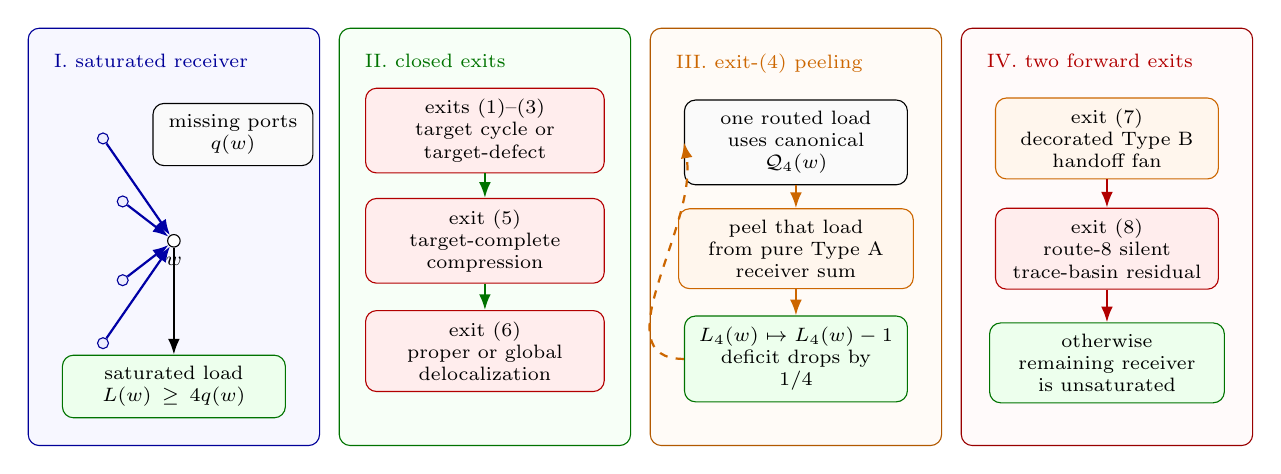
\begin{tikzpicture}[
pt/.style={circle,draw,fill=white,inner sep=1.6pt},
load/.style={circle,draw=blue!60!black,fill=blue!7,inner sep=1.4pt},
box/.style={rectangle,rounded corners,draw,fill=black!2,align=center,inner sep=4pt,text width=2.55cm},
good/.style={rectangle,rounded corners,draw=green!45!black,fill=green!7,align=center,inner sep=4pt,text width=2.55cm},
warn/.style={rectangle,rounded corners,draw=orange!80!black,fill=orange!7,align=center,inner sep=4pt,text width=2.55cm},
bad/.style={rectangle,rounded corners,draw=red!70!black,fill=red!7,align=center,inner sep=4pt,text width=2.55cm},
arr/.style={-{Latex[length=2mm]},thick},
dasharr/.style={-{Latex[length=2mm]},thick,dashed},
every node/.style={font=\scriptsize}
]
\draw[rounded corners,fill=blue!3,draw=blue!60!black] (-7.75,-2.75) rectangle (-4.05,2.55);
\draw[rounded corners,fill=green!3,draw=green!45!black] (-3.80,-2.75) rectangle (-0.10,2.55);
\draw[rounded corners,fill=orange!3,draw=orange!70!black] (0.15,-2.75) rectangle (3.85,2.55);
\draw[rounded corners,fill=red!2,draw=red!60!black] (4.10,-2.75) rectangle (7.80,2.55);
\node[anchor=north west,blue!60!black] at (-7.55,2.35) {I. saturated receiver};
\node[anchor=north west,green!45!black] at (-3.60,2.35) {II. closed exits};
\node[anchor=north west,orange!80!black] at (0.35,2.35) {III. exit-(4) peeling};
\node[anchor=north west,red!70!black] at (4.30,2.35) {IV. two forward exits};

\node[pt,label=below:\(w\)] (w) at (-5.90,-0.15) {};
\node[load] (u1) at (-6.80,1.15) {};
\node[load] (u2) at (-6.55,0.35) {};
\node[load] (u3) at (-6.55,-0.65) {};
\node[load] (u4) at (-6.80,-1.45) {};
\draw[arr,blue!65!black] (u1)--(w);
\draw[arr,blue!65!black] (u2)--(w);
\draw[arr,blue!65!black] (u3)--(w);
\draw[arr,blue!65!black] (u4)--(w);
\node[box,text width=1.75cm] at (-5.15,1.20) {missing ports\\\(q(w)\)};
\node[good,text width=2.55cm] (sat) at (-5.90,-2.00) {saturated load\\\(L(w)\ge4q(w)\)};
\draw[arr] (w)--(sat);

\node[bad,text width=2.75cm] (target) at (-1.95,1.25) {exits (1)--(3)\\target cycle or\\target-defect};
\node[bad,text width=2.75cm] (comp) at (-1.95,-0.15) {exit (5)\\target-complete\\compression};
\node[bad,text width=2.75cm] (deloc) at (-1.95,-1.55) {exit (6)\\proper or global\\delocalization};
\draw[arr,green!45!black] (target)--(comp);
\draw[arr,green!45!black] (comp)--(deloc);

\node[box,text width=2.55cm] (load4) at (2.00,1.10) {one routed load\\uses canonical\\\(\mathcal Q_4(w)\)};
\node[warn,text width=2.70cm] (peel) at (2.00,-0.25) {peel that load\\from pure Type A\\receiver sum};
\node[good,text width=2.55cm] (less) at (2.00,-1.65) {\(L_4(w)\mapsto L_4(w)-1\)\\deficit drops by\\\(1/4\)};
\draw[arr,orange!80!black] (load4)--(peel);
\draw[arr,orange!80!black] (peel)--(less);
\draw[dasharr,orange!80!black] (less.west) to[out=180,in=-80] (load4.west);

\node[warn,text width=2.55cm] (handoff) at (5.95,1.15) {exit (7)\\decorated Type B\\handoff fan};
\node[bad,text width=2.55cm] (route8) at (5.95,-0.25) {exit (8)\\route-8 silent\\trace-basin residual};
\node[good,text width=2.70cm] (unsat) at (5.95,-1.70) {otherwise\\remaining receiver\\is unsaturated};
\draw[arr,red!70!black] (handoff)--(route8);
\draw[arr,red!70!black] (route8)--(unsat);
\end{tikzpicture}%
}
\caption[Visual proof of the Type A saturated-exit drain]{Visual proof of the Type A saturated-exit drain.  Panel I shows a Type A receiver \(w\) with missing-port count \(q(w)=3-d_X(w)\) and saturated routed load \(L(w)\ge4q(w)\).  Panel II records the exits that close inside the Type A analysis: exits (1)--(3) create a target cycle or target-defective state, exit (5) gives target-complete compression, and exit (6) gives proper or global delocalization.  Panel III isolates exit (4): one routed load using the canonical family \(\mathcal Q_4(w)\) is peeled out of the pure Type A receiver sum, changing \(L_4(w)\) to \(L_4(w)-1\) and reducing the remaining receiver deficit by \(1/4\); the dashed loop indicates that the receiver is then tested again with smaller residual load.  Panel IV shows the two forward exits: exit (7) is reclassified as decorated Type B handoff fan data, while exit (8) is the route-8 trace-basin residual treated by the later carrier-reduction and no-go figures.}
\label{fig:typeA-saturated-exit-drain}
\end{figure}

\begin{lemma}[Saturated receiver handoff]\label[lemma]{lem:typeA-saturated-handoff}
Let $X$ be a Type A support.  If a receiver $w$ satisfies
$L(w)\ge4q(w)$, then repeated application of the saturated receiver routing has
one of the following outcomes: a closed exit among (1)--(3), (5), and (6)
occurs; the Type B handoff exit (7) occurs; the route-8 residual profile of
\cref{def:typeA-silent-core-residual} occurs; or exit (4) peels finitely many
routed loads and the remaining receiver load becomes unsaturated.  Consequently
every receiver that remains in the pure Type A discharging branch after the
closed exits, exit-(4) peeling, route 8, and the Type B handoff have been removed
satisfies
\[
L(w)\le4q(w)-1.
\]
\end{lemma}

\begin{proof}
Start with the empty peeling set \(P_4(w)=\varnothing\).  If the residual load
\(L_4(w)\) is at most \(4q(w)-1\), the receiver is already unsaturated in the
remaining Type A charge calculation.  Otherwise
\cref{lem:typeA-exit4-residual-routing} applies to the unpeeled loads.  Exits
(1)--(3), (5), and (6) close by \cref{lem:typeA-exits-discharged}; exit (7) is
transferred to the decorated handoff fan branch by the same lemma; and exit (8)
is the route-8 residual profile.  If exit (4) occurs, then
\cref{lem:typeA-exit4-discharge} enlarges \(P_4(w)\) by one routed load, so
\(L_4(w)\) decreases by one.  Since \(\mathcal L(w)\) is finite, this exit-(4)
peeling step cannot occur indefinitely.  Therefore the iteration ends in one of
the listed outcomes.  A receiver that remains in the pure Type A discharging
branch is precisely one for which the iteration ended by reaching
\(L_4(w)\le4q(w)-1\); with all peeled loads removed from that branch, this is the
displayed unsaturated bound.
\end{proof}

\begin{remark}[Use of exit-(4) peeling]\label[remark]{rem:typeA-exit4-peeling-use}
The peeling set is a routing record.  A load in \(P_4(w)\) exits through the
target-defect branch before the pure Type A charge is summed.  The charge
calculation therefore applies only to the unpeeled loads counted by \(L_4(w)\).
Consequently \cref{lem:typeA-exclusion} is invoked only after the target-defect
alternative has been removed; a support with a remaining exit-(4) witness is
routed by alternative (iii) of \cref{lem:density-mersenne}.
\end{remark}

\begin{remark}[Type A--Type B stratification]\label[remark]{rem:typeA-typeB-stratification}
The saturated Type A analysis
\[
\cref{lem:typeA-visible-entry,lem:typeA-silent-excess,lem:typeA-exits-discharged,lem:typeA-saturated-handoff,lem:typeA-unsaturated-discharge}
\]
uses no conclusion of \cref{lem:typeB-exclusion}.  The only Type B reference in
that block is the handoff interface:
\cref{lem:typeA-high-degree-handoff,lem:decorated-fan-admissibility} construct
and validate the decorated envelope data.  The logical direction then reverses:
\cref{lem:typeB-exclusion} may apply the completed Type A saturated and
unsaturated conclusions to the post-ledger core.

The possible alternation terminates.  Type A handoffs are assigned to grouped
decorated envelopes by the connected components of the core--center incidence
graph in \cref{def:decorated-typeB-envelope-support}.  Each such component
uses its finite set of center tokens once in the grouped-envelope ledger.  After
the Type B ledger removes the corresponding fan/envelope entries, the remaining
core is a proper subcore of the previous support or has fewer unused incidence
component tokens.  Since the support and center-token sets are finite, an
\(A\to B\to A\) alternation cannot continue indefinitely.
\end{remark}

\begin{lemma}[Unsaturated Type A discharging]\label[lemma]{lem:typeA-unsaturated-discharge}
Let $X$ be a Type A support in which every receiver satisfies
$L(w)\le4q(w)-1$.  Then
\[
\defp(X)\ge\frac14|V(X)|.
\]
Equivalently, if $n_i=|\{v\in V(X):d_X(v)=i\}|$, then
\[
n_3\le3n_2+7n_1+11n_0.
\]
\end{lemma}

\begin{proof}
Set
\[
\ch(v)=(3-d_X(v))-\frac14 .
\]
Then $\sum_v\ch(v)=\defp(X)-|V(X)|/4$.  A cubic vertex has charge
$-1/4$, and every cubic vertex is assigned to exactly one receiver by
\cref{lem:typeA-receiver-loads}.  A receiver $w$ has initial charge
$q(w)-1/4$ and pays $1/4$ for each assigned cubic vertex.  The unsaturated
bound gives
\[
q(w)-\frac14-\frac14L(w)\ge
q(w)-\frac14-\frac14(4q(w)-1)=0 .
\]
All other non-cubic vertices have nonnegative charge and pay nothing.  Hence
the final total charge is nonnegative, so
$\defp(X)-|V(X)|/4\ge0$.  Written by degree classes, the receiver capacities
are $3,7,11$ for internal degrees $2,1,0$, which is exactly
$n_3\le3n_2+7n_1+11n_0$.
\end{proof}

\begin{lemma}[Density forces discharging, target defect, Type B handoff, or route 8]\label[lemma]{lem:density-mersenne}
Let $X$ be a connected admissible support (\cref{def:admissible}) with
$\sigma(X)=0$.  Thus $X$ is contextually dyadic-safe
(\cref{def:dyadic-safe}), $P_{13}$-free, has empty internal $3$-core, has every
deficient vertex supplied from the packing $W$ (\cref{lem:stub-positive}), and
is hereditarily target-uncompressible (\cref{cor:uncompressible}).  Then one of
the following holds:
\begin{enumerate}[label=(\roman*), leftmargin=2.2em]
\item
\[
\defp(X)\ge\tfrac14|V(X)|,
\qquad\text{equivalently}\qquad
\frac{2|E(X)|}{|V(X)|}\le 2.75 .
\]
\item $X$ produces a decorated handoff fan envelope in the sense of
\cref{def:decorated-fan-envelope}.
\item $X$ has an exit-(4) witness for a routed load in the sense of
\cref{def:typeA-exit4-peeling}; this branch is routed to the target-defect exit
and that routed load is removed from the Type A receiver calculation by
\cref{lem:typeA-exit4-discharge}.
\item $X$ contains an admissible silent-core residual profile in the sense of
\cref{def:typeA-silent-core-residual}.
\end{enumerate}
\end{lemma}

\begin{proof}
If a receiver is saturated, \cref{lem:typeA-saturated-handoff} applies.  Exits
(1)--(3), (5), and (6) contradict the standing target, replacement, or
delocalization invariants.  Exit (4) gives alternative (iii) and peels one
routed load by \cref{lem:typeA-exit4-discharge}.  Exit (7) gives alternative
(ii), and exit (8) gives alternative (iv).  If no saturated receiver remains
after excluding alternatives (ii)--(iv), every receiver in the pure Type A
support is unsaturated.  The charge calculation of
\cref{lem:typeA-unsaturated-discharge} gives
\[
\defp(X)\ge\frac14|V(X)|.
\]
Since $\sigma(X)=0$, this is equivalent to
$2|E(X)|/|V(X)|\le2.75$.
\end{proof}

\begin{lemma}[Type A split and charge bound]\label[lemma]{lem:typeA-exclusion}
Let $X$ be a connected admissible support with $\sigma(X)=0$, empty internal
$3$-core, $P_{13}$-free and dyadic-safe.  If $X$ contains no exit-(4) witness for
a routed load and contains neither an admissible silent-core residual profile nor
a decorated handoff fan envelope, then
\[
\defp(X)\ge\frac14|V(X)| ,
\qquad\text{equivalently}\qquad
\frac{2|E(X)|}{|V(X)|}\le 2.75 ,
\]
so that $\No(X)\ge0$.  Consequently a Type A support with $\No(X)<0$ must carry
an admissible route-8 residual profile, produce the Type B handoff, or contain
an exit-(4) witness for a routed load.
\end{lemma}

\begin{proof}
The hypotheses are the admissibility hypotheses used in
\cref{lem:density-mersenne}.  Since the route-8 residual and Type B handoff
alternatives and the exit-(4) witness alternative are excluded by hypothesis,
that lemma gives
$\defp(X)\ge\tfrac14|V(X)|$.  Since $\sigma(X)=0$,
\[
\No(X)=\defp(X)-\frac14|V(X)|\ge0.
\]
Thus a Type A support outside the route-8 residual class, outside the Type B
handoff, and outside the exit-(4) target-defect exit cannot have negative net
charge.
\end{proof}

\begin{definition}[Large-budget Type A deficit]\label[definition]{def:typeA-large-budget-deficit}
Let $\mathcal X$ be a collection of Type A supports whose saturated receivers
survive only through the route-8 residual profile of
\cref{def:typeA-silent-core-residual}.  Put
\[
D_A(\mathcal X)=
\sum_{X\in\mathcal X}\left(\frac14|V(X)|-\defp(X)\right).
\]
The collection $\mathcal X$ \emph{carries the large-budget Type A deficit} if
\[
D_A(\mathcal X)\ge
\left(\frac14-\tau_{\rm win}\right)|R|-o(|R|).
\]
\end{definition}

\begin{lemma}[Quantitative burden of the reduced route-8 residual]\label[lemma]{lem:typeA-route8-burden}
Let $\mathcal X$ be a collection of Type A supports whose saturated receivers
survive only through the route-8 residual profile of
\cref{def:typeA-silent-core-residual}; in particular, no receiver in any
$X\in\mathcal X$ realizes exits (1)--(7).  Let $D_A(\mathcal X)$ be as in
\cref{def:typeA-large-budget-deficit}.  Let
\[
N_{\rm basin}(\mathcal X)=
\sum_{X\in\mathcal X}\sum_w |\mathcal U_X(w)|,
\]
where $w$ ranges over the saturated route-8 receivers of $X$ and
$\mathcal U_X(w)$ denotes the unpaid silent routed vertices at $w$.  Thus
$N_{\rm basin}$ counts the indexed trace-basin entries $(u,B_u)$; two different
vertices may contribute two entries even if their underlying boundaried
subgraphs coincide.  Then
\[
N_{\rm basin}(\mathcal X)\ge4D_A(\mathcal X).
\]
Consequently, if $\mathcal X$ carries the large-budget Type A deficit, then
it contains at least
\[
4\left(\frac14-\tau_{\rm win}\right)|R|-o(|R|)
\]
indexed trace-basin entries.  In the limiting window-only cap this coefficient
is
\[
4\left(\frac14-0.22817486846\ldots\right)
=0.08730052616\ldots .
\]
\end{lemma}

\begin{proof}
For each $X\in\mathcal X$, the absence of exits (1)--(7) implies in particular
that no saturated receiver has a completion port carrying four visible
receiver-entry returns.  Hence
\cref{lem:typeA-silent-excess-count} applies to $X$ and gives
\[
S_{\rm sil}^{\rm exc}(X)\ge
4\left(\frac14|V(X)|-\defp(X)\right).
\]
By \cref{lem:typeA-reduced-silent-residual}, every unpaid silent excess vertex
counted by $S_{\rm sil}^{\rm exc}(X)$ has a target-complete-minimal trace basin
unless one of exits (4)--(7) occurs.  Those exits are absent by hypothesis.
Counting the resulting indexed pairs $(u,B_u)$ and summing the displayed
inequality over $X\in\mathcal X$ proves
$N_{\rm basin}(\mathcal X)\ge4D_A(\mathcal X)$.  No distinctness of the
underlying subgraphs $B_u$ is used.

If $\mathcal X$ carries the large-budget Type A deficit, then
\[
D_A(\mathcal X)\ge
\left(\frac14-\tau_{\rm win}\right)|R|-o(|R|)
\]
by \cref{def:typeA-large-budget-deficit}.  Multiplying by the factor $4$ from
the first part gives the stated lower bound.  Substituting
$\tau_{\rm win}=0.22817486846\ldots$ gives the displayed coefficient.
\end{proof}

\begin{definition}[Route-8 response carriers and two-carrier entries]\label[definition]{def:typeA-route8-carriers}
Let $\mathcal X$ be a collection of Type A supports whose saturated receivers
survive only through route 8.  For a Type A support $X$, put
\[
\partial_E X
=\{(x,xy):x\in V(X),\ y\notin V(X),\ xy\in E(G)\},
\]
the set of oriented boundary incidences leaving $X$.  Since $\sigma(X)=0$,
every vertex of $X$ has ambient degree $3$, and hence
\[
	|\partial_E X|=\defp(X).
	\]

	For an indexed entry \(\xi=(X,w,u,B_u)\), every declared \(u\)-supported
	coordinate of \(\rho_u(B_u)\) that uses the ambient exterior of \(X\) records
	the oriented boundary incidence of \(X\) through which it leaves \(X\).  More
	precisely, the declared support of such a coordinate contains a completion-port
	incidence, first-entry incidence, connector-band endpoint, boundary-degree
	entry, or packed-window interface incidence; when that incidence is represented
	by an edge \(xy\in E(G)\) with \(x\in V(X)\) and \(y\notin V(X)\), its
	\emph{ambient carrier} is the element \(c=(x,xy)\in\partial_E X\).  Incidences
	of \(\partial B_u\) internal to \(X\) have no ambient carrier unless the
	declared coordinate canonically assigns them to the terminal completion port of
	\(T_u\), in which case the carrier is that completion-port incidence.  Thus
	ambient carriers are not extra data attached to \(B_u\); they are the
	\(\partial_E X\)-labels already recorded by the declared coordinate signature.

	An indexed route-8 entry is a tuple
	\[
	\xi=(X,w,u,B_u),
	\]
	where $u\in\mathcal U_X(w)$ and $B_u$ is the target-complete-minimal trace
	basin assigned to $u$.  The set of all indexed route-8 entries of
	\(\mathcal X\) is denoted
	\[
	\Xi(\mathcal X).
	\]
	More generally, a \emph{tagged Type A entry family} is any finite family
	\(\mathfrak E\) of tuples \(\xi=(X,w,u,B_u)\) with \(\sigma(X)=0\),
	\(u\in\mathcal U_X(w)\), and \(B_u\) the trace basin assigned to \(u\).
	Target-complete-minimality is required only when \(\xi\) is called a route-8
	entry.  The carrier constructions below apply to every
	\(\xi\in\mathfrak E\).  For a pure route-8 collection the tagged family is
	\(\mathfrak E=\Xi(\mathcal X)\).
	A boundary incidence $c\in\partial_E X$ is
	\emph{active for $\xi$} if the declared support of a $u$-supported coordinate
in $\rho_u(B_u)$ contains \(c\) as a completion-port incidence, first-entry
incidence, connector-band endpoint, boundary-degree entry, or packed-window
interface incidence under \cref{def:declared-coordinate-signature}.

For a coordinate $r\in\mathcal R_u(B_u)$, let
\[
\operatorname{car}_\xi(r)\subseteq\partial_E X
\]
be the set of active carriers used by the declared support of $r$.  If
$D\subseteq\partial_E X$, the \emph{$D$-restriction}
$\rho_u(B_u)|_D$ is the response quotient obtained from $\rho_u(B_u)$ by
retaining the full boundary degree profile $\mathbf d_\partial(B_u)$ and
retaining, apart from this boundary-degree profile, exactly those
$u$-supported coordinates $r$ with
$\operatorname{car}_\xi(r)\subseteq D$; all other $u$-supported coordinates are
forgotten.  Thus every carrier restriction is taken inside the original
boundary-degree fibre.

A set $D\subseteq\partial_E X$ is a \emph{target-complete carrier set for
$\xi$} if the quotient
\[
\rho_u(B_u)\longrightarrow \rho_u(B_u)|_D
\]
is target-complete in the sense of \cref{def:typeA-trace-basin}: for every
outside context compatible with the boundary profile, all realizations of
$\rho_u(B_u)|_D$ give the same target predicate as $\rho_u(B_u)$ after gluing.
Such sets exist: for $D=\partial_E X$, all declared $u$-supported coordinates
are retained, so the completeness clause in \cref{def:typeA-trace-basin}
applies.  Let
\[
\mathcal C_{\rm ess}(\xi)
\]
be the lexicographically first inclusion-minimal target-complete carrier set for
$\xi$.  Its elements are the \emph{essential carriers} of $\xi$, and the
carriers in $\partial_E X\setminus\mathcal C_{\rm ess}(\xi)$ are
\emph{noncore carriers}.  Thus
\[
\rho_u(B_u)\longrightarrow
\rho_u(B_u)|_{\mathcal C_{\rm ess}(\xi)}
\]
is target-complete by definition, while for every
$c\in\mathcal C_{\rm ess}(\xi)$ the smaller restriction
$\rho_u(B_u)|_{\mathcal C_{\rm ess}(\xi)\setminus\{c\}}$ is not
target-complete.  Put
\[
\alpha_{\mathfrak E}(\xi)=|\mathcal C_{\rm ess}(\xi)|.
\]
The value is independent of \(\mathfrak E\); the subscript records the current
branch state in which privacy is evaluated.

An essential carrier for $\xi$ is \emph{private for $\xi$ relative to
\(\mathfrak E\)} if it is not essential for any other tagged entry in
\(\mathfrak E\).  Let
\[
\pi_{\mathfrak E}(\xi)
\]
be the number of private essential carriers of $\xi$ relative to
\(\mathfrak E\).  When \(\mathfrak E=\Xi(\mathcal X)\), abbreviate these
quantities by \(\alpha_{\mathcal X}(\xi)\) and
\(\pi_{\mathcal X}(\xi)\).

The tagged entry $\xi$ is \emph{two-carrier relative to \(\mathfrak E\)} if
\[
\pi_{\mathfrak E}(\xi)\le2.
\]
When \(\mathfrak E=\Xi(\mathcal X)\) and \(\xi\) is a route-8 entry, this is
called a \emph{two-carrier route-8 entry}.
	An admissible \emph{two-carrier route-8 residual} is a large-budget route-8
	collection containing such an entry.
	\end{definition}

\begin{definition}[Canonical exit-(4) quotient family]\label[definition]{def:typeA-exit4-family}
Let \(w\) be a saturated receiver in a Type A support \(X\).  Write
\(\mathcal Q_4^{\rm pre}(w)\) for the boundary-degree-preserving response
quotients generated by clauses \textup{(Q1)}--\textup{(Q4)} below; these
clauses do not use carrier or privacy data.  Every bare occurrence of
\(\mathcal Q_4(w)\) before a tagged family is fixed denotes this preliminary
family.

For the collection-dependent clause \textup{(Q5)}, freeze the entire current
tagged Type A entry family \(\mathfrak E\); in particular, \(\mathfrak E\)
contains every current entry at \(w\).  Then
\(\mathcal Q_4(w;\mathfrak E)\) is the union of
\(\mathcal Q_4^{\rm pre}(w)\) and the quotients generated by clause
\textup{(Q5)}.  For a pure route-8 collection \(\mathcal X\), the notation
\(\mathcal Q_4(w;\mathcal X)\) means
\(\mathcal Q_4(w;\Xi(\mathcal X))\).
\begin{enumerate}[label=(Q\arabic*), leftmargin=2.2em]
\item the visible receiver-entry coordinate identifications tested in
\cref{lem:typeA-visible-entry};
\item the silent/excess boundary-response quotient of the basin \(B(w)\) in
\cref{lem:typeA-silent-excess};
\item the trace-local non-carrier quotient or identification of a trace basin
in the sense of \cref{def:typeA-trace-basin}, as used in
\cref{lem:typeA-reduced-silent-residual};
\item the finite continuation or cubic-switch quotient produced by
\cref{lem:typeA-continuation-routing,lem:typeA-cubic-switch-absorption};
\item for an indexed route-8 entry
\(\xi=(X,w,u,B_u)\in\mathfrak E\), the carrier-deletion quotient
\[
\rho_u(B_u)|_{\mathcal C_{\rm ess}(\xi)}
\longrightarrow
\rho_u(B_u)|_{\mathcal C_{\rm ess}(\xi)\setminus\{c\}}
\]
when \(c\in\mathcal C_{\rm ess}(\xi)\), the entry is two-carrier relative to
the frozen tagged family, \(\pi_{\mathfrak E}(\xi)\le2\), and the
distinguishing event is recorded by a
declared deletion witness in the sense of
\cref{def:typeA-carrier-deletion-witness}.
\end{enumerate}
Every member of \(\mathcal Q_4^{\rm pre}(w)\), and every member of
\(\mathcal Q_4(w;\mathfrak E)\), retains the boundary degree profile of the
response state on which it is defined.  At the preliminary stage, exit (4)
occurs precisely when a quotient in \(\mathcal Q_4^{\rm pre}(w)\) is
target-defective.  After \(\mathfrak E\) is frozen, the Q5 refinement tests the
additional members of \(\mathcal Q_4(w;\mathfrak E)\).  The declared routed-load
support is part of the canonical construction: in \textup{(Q1)} it is the set of
visible routed loads whose response coordinates are identified; in
\textup{(Q2)} it is the routed loads in the basin \(B(w)\); in \textup{(Q3)} it
is the trace load \(u\) whose basin is being tested; in \textup{(Q4)} it is the
routed loads whose declared connector coordinates form the finite family
\(\mathcal K\); and in \textup{(Q5)} it is the indexed load \(u\) of the
route-8 entry \(\xi=(X,w,u,B_u)\).
\end{definition}

\begin{definition}[True route-8 residual entries]\label[definition]{def:typeA-true-route8-residual}
Let \(\mathfrak E\) be a frozen tagged Type A entry family and let
\(\xi=(X,w,u,B_u)\in\mathfrak E\) be an indexed route-8 entry.  The entry is a
\emph{preliminary route-8 entry} when \(w\) is saturated, its data form an
admissible silent-core residual profile, \(B_u\) is target-complete-minimal,
exits \textup{(1)}--\textup{(3)} and \textup{(5)}--\textup{(7)} are absent,
and exit \textup{(4)} is absent for clauses \textup{(Q1)}--\textup{(Q4)} of
\cref{def:typeA-exit4-family}.

After \(\mathfrak E\), its essential carrier sets, and the privacy counts
\(\pi_{\mathfrak E}\) have been fixed, perform the \emph{Q5 refinement}:
\begin{enumerate}[label=(Q5\alph*), leftmargin=2.6em]
\item if a clause-\textup{(Q5)} quotient in
\(\mathcal Q_4(w;\mathfrak E)\) is target-defective, the entry leaves through
exit \textup{(4)}, with the indexed load \(u\) as its declared routed-load
support;
\item if no clause-\textup{(Q5)} quotient is target-defective, record Q5
absence.
\end{enumerate}
The test changes only the branch tag.  It does not alter \(G\), the support,
the trace basin, the carrier sets, the privacy counts, the receiver burden, or
any previously recorded absent exit.

A preliminary route-8 entry on the Q5-absent branch is a \emph{true route-8
residual entry}.  Equivalently, it satisfies:
\begin{enumerate}[label=(R\arabic*), leftmargin=2.2em]
\item \(w\) is a saturated receiver of \(X\);
\item exits (1)--(7) of \cref{def:typeA-saturated-exits} are absent at \(w\),
with exit (4) interpreted through the refined canonical family
\(\mathcal Q_4(w;\mathfrak E)\);
\item the data at \(w\) form an admissible silent-core residual profile of
\cref{def:typeA-silent-core-residual}; and
\item \(B_u\) is the target-complete-minimal trace basin assigned to \(u\).
\end{enumerate}
For a route-8 Type A collection \(\mathcal X\), take
\(\mathfrak E=\Xi(\mathcal X)\).  It is a \emph{true route-8 residual
collection} when every indexed entry lies on the Q5-absent branch.  Thus, in a
true route-8 residual entry, any occurrence of one of exits (1)--(7)
contradicts the definition of the residual.
\end{definition}

	\begin{figure}[t]
	\centering
\resizebox{0.98\textwidth}{!}{%
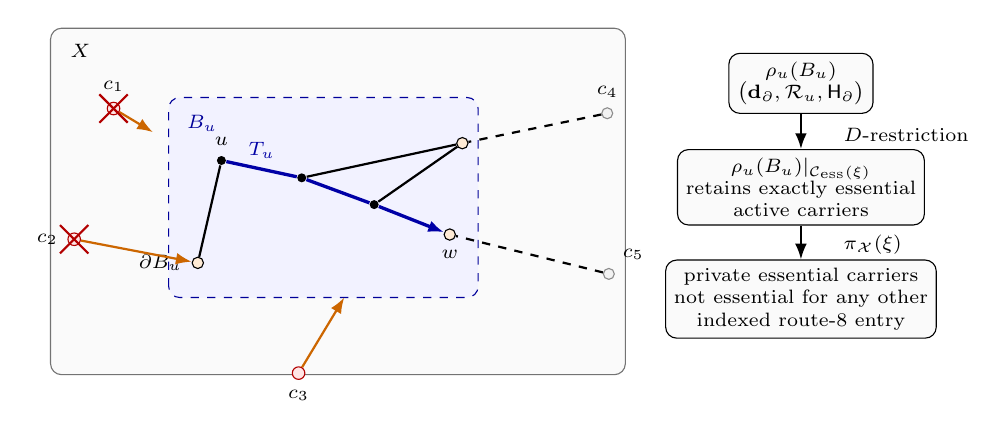
\begin{tikzpicture}[
vtx/.style={circle,fill=black,inner sep=1.15pt},
bv/.style={circle,draw,fill=orange!16,inner sep=1.45pt},
ess/.style={circle,draw=red!70!black,fill=red!10,inner sep=1.6pt},
noncore/.style={circle,draw=black!45,fill=black!5,inner sep=1.4pt},
edge/.style={thick},
trace/.style={-{Latex[length=2mm]},very thick,blue!65!black},
car/.style={-{Latex[length=2mm]},thick,orange!80!black},
coord/.style={rectangle,rounded corners,draw,align=center,inner sep=3pt,fill=black!2},
every node/.style={font=\scriptsize}
]
\draw[rounded corners,fill=black!2,draw=black!55] (-4.35,-2.20) rectangle (2.95,2.20);
\node[anchor=north west] at (-4.22,2.12) {$X$};
\draw[rounded corners,fill=blue!5,draw=blue!60!black,dashed] (-2.85,-1.22) rectangle (1.08,1.32);
\node[anchor=north west,blue!60!black] at (-2.74,1.22) {$B_u$};

\node[vtx,label=above:$u$] (u) at (-2.18,0.52) {};
\node[vtx] (a) at (-1.16,0.30) {};
\node[vtx] (b) at (-0.24,-0.04) {};
\node[bv,label=below:$w$] (w) at (0.72,-0.42) {};
\node[bv,label=left:$\partial B_u$] (pb1) at (-2.48,-0.78) {};
\node[bv] (pb2) at (0.88,0.74) {};
\draw[trace] (u)--node[above]{$T_u$}(a)--(b)--(w);
\draw[edge] (pb1)--(u);
\draw[edge] (pb2)--(a);
\draw[edge] (b)--(pb2);

\node[ess,label=above:$c_1$] (c1) at (-3.55,1.18) {};
\node[ess,label=left:$c_2$] (c2) at (-4.05,-0.48) {};
\node[ess,label=below:$c_3$] (c3) at (-1.20,-2.18) {};
\node[noncore,label=above:$c_4$] (c4) at (2.72,1.12) {};
\node[noncore,label=above right:$c_5$] (c5) at (2.74,-0.92) {};
\draw[car] (c1)--(-3.05,0.88);
\draw[car] (c2)--(pb1);
\draw[car] (c3)--(-0.62,-1.22);
\draw[edge,dashed] (c4)--(pb2);
\draw[edge,dashed] (c5)--(w);

\node[coord] (rho) at (5.18,1.50) {$\rho_u(B_u)$\\$\bigl(\mathbf d_\partial,\mathcal R_u,\profile_\partial\bigr)$};
\node[coord] (core) at (5.18,0.18) {$\rho_u(B_u)|_{\mathcal C_{\rm ess}(\xi)}$\\retains exactly essential\\active carriers};
\node[coord] (priv) at (5.18,-1.24) {private essential carriers\\not essential for any other\\indexed route-8 entry};
\draw[-{Latex[length=2mm]},thick] (rho)--(core);
\node[anchor=west,fill=white,inner sep=1pt] at (5.68,0.84) {$D$-restriction};
\draw[-{Latex[length=2mm]},thick] (core)--(priv);
\node[anchor=west,fill=white,inner sep=1pt] at (5.68,-0.55) {$\pi_{\mathcal X}(\xi)$};

\draw[red!70!black,thick] ($(c1)+(-0.18,0.18)$) -- ($(c1)+(0.18,-0.18)$);
\draw[red!70!black,thick] ($(c1)+(-0.18,-0.18)$) -- ($(c1)+(0.18,0.18)$);
\draw[red!70!black,thick] ($(c2)+(-0.18,0.18)$) -- ($(c2)+(0.18,-0.18)$);
\draw[red!70!black,thick] ($(c2)+(-0.18,-0.18)$) -- ($(c2)+(0.18,0.18)$);
\end{tikzpicture}%
}
\caption[Visual definition of a route-8 trace-basin entry]{Visual definition of a route-8 trace-basin entry and its carrier core.  The grey rectangle is the Type A support $X$, and the blue dashed shaded region is the target-complete-minimal trace basin $B_u\subseteq X$ assigned to the routed vertex $u$.  Black edges are support edges inside \(X\), the blue arrowed path $T_u$ is the canonical trace from $u$ to the receiver $w$, and $\partial B_u$ denotes the boundary of the basin inside $X$.  The entry is $\xi=(X,w,u,B_u)$.  The labels $c_1,\ldots,c_5$ denote oriented boundary incidences in $\partial_E X$.  Orange arrows mark active carrier incidences used by declared $u$-supported coordinates; dashed black incidences illustrate boundary incidences that remain outside the essential core.  Red carrier nodes are elements of the essential carrier set $\mathcal C_{\rm ess}(\xi)$, grey carrier nodes are noncore carriers, and the red crosses on $c_1,c_2$ mark carriers counted as private for this indexed entry inside the collection $\mathcal X$.  The response state $\rho_u(B_u)$ records the boundary degree profile $\mathbf d_\partial$, the $u$-supported response coordinates $\mathcal R_u$, and the boundary target profile $\profile_\partial$.  A $D$-restriction keeps only the coordinates whose declared carriers lie in the chosen set $D$; the displayed restriction uses $D=\mathcal C_{\rm ess}(\xi)$.  The number $\pi_{\mathcal X}(\xi)$ counts the private essential carriers of $\xi$, and a two-carrier route-8 entry is one with $\pi_{\mathcal X}(\xi)\le2$.}
\label{fig:typeA-route8-carrier-gadget}
\end{figure}

\begin{definition}[Carrier-deletion witnesses]\label[definition]{def:typeA-carrier-deletion-witness}
Let
\[
\xi=(X,w,u,B_u)
\]
be an indexed route-8 entry, and put
\[
\mathcal C=\mathcal C_{\rm ess}(\xi).
\]
For \(c\in\mathcal C\), the \emph{\(c\)-deletion quotient} is the quotient
\[
q_{\xi,c}:\rho_u(B_u)|_{\mathcal C}\longrightarrow
\rho_u(B_u)|_{\mathcal C\setminus\{c\}} .
\]
A \emph{\(c\)-deletion witness} is a realization \(S\) of
\(\rho_u(B_u)|_{\mathcal C\setminus\{c\}}\), together with a compatible outside
context \(Y\), such that
\[
S\oplus Y
\]
has a different target predicate from the original core state
\(\rho_u(B_u)|_{\mathcal C}\) glued to the corresponding context.  A witnessing
target event is chosen as the lexicographically first simple edge-rooted return
or simple cycle responsible for this target difference.  The \emph{declared
support} of the witness is the finite set of declared response coordinates from
\cref{def:declared-coordinate-signature} used by that event, and its
\emph{carrier support} is the union of the ambient carriers of those coordinates
in \(\partial_E X\).  The witness is \emph{internal} when this event uses an edge
of \(B_u-\partial B_u\).  It is \emph{mixed} when, in addition, the event uses an
edge outside \(X\).
\end{definition}

\begin{lemma}[Essential carriers have deletion witnesses]\label[lemma]{lem:typeA-essential-deletion-witness}
Let \(\xi=(X,w,u,B_u)\) be an indexed route-8 entry.  For every
\[
c\in\mathcal C_{\rm ess}(\xi),
\]
the \(c\)-deletion quotient \(q_{\xi,c}\) is not target-complete.  Equivalently,
there exists a \(c\)-deletion witness in the sense of
\cref{def:typeA-carrier-deletion-witness}.
\end{lemma}

\begin{proof}
By definition, \(\mathcal C_{\rm ess}(\xi)\) is inclusion-minimal among
target-complete carrier sets for \(\xi\).  Therefore
\[
\mathcal C_{\rm ess}(\xi)\setminus\{c\}
\]
is not a target-complete carrier set.  The full-to-core quotient
\[
\rho_u(B_u)\longrightarrow \rho_u(B_u)|_{\mathcal C_{\rm ess}(\xi)}
\]
is target-complete.  If \(q_{\xi,c}\) were target-complete, then
\cref{lem:target-complete-quotient-composition} would make the composite
\[
\rho_u(B_u)\longrightarrow
\rho_u(B_u)|_{\mathcal C_{\rm ess}(\xi)\setminus\{c\}}
\]
target-complete, contradicting the preceding sentence.  Hence \(q_{\xi,c}\) is
not target-complete.  Unwinding the definition of target-completeness gives a
compatible outside context and a realization of the smaller restricted response
state with different target predicate.  Choosing the lexicographically first
simple edge-rooted return or simple cycle that accounts for the difference gives
the stated deletion witness.
\end{proof}

\begin{lemma}[Deletion witnesses are declared]\label[lemma]{lem:typeA-deletion-witness-declared}
Let \(\xi=(X,w,u,B_u)\) be an indexed route-8 entry, and let
\(c\in\mathcal C_{\rm ess}(\xi)\).  Every \(c\)-deletion witness obtained from
\cref{lem:typeA-essential-deletion-witness} has declared support and carrier
support in the sense of \cref{def:typeA-carrier-deletion-witness}.  Moreover its
carrier support contains \(c\).
\end{lemma}

\begin{proof}
The witness distinguishes the core state
\(\rho_u(B_u)|_{\mathcal C_{\rm ess}(\xi)}\) from the smaller restriction
\(\rho_u(B_u)|_{\mathcal C_{\rm ess}(\xi)\setminus\{c\}}\) in a compatible
outside context.  If the witnessing target event used only retained coordinates,
then its truth value would be the same in the two glued states, because the two
states agree on every retained declared \(u\)-supported coordinate and on the
full boundary degree profile.  Hence the event uses at least one coordinate
forgotten by the deletion quotient.

By the definition of \(D\)-restriction in \cref{def:typeA-route8-carriers}, the
coordinates forgotten when passing from
\(\mathcal C_{\rm ess}(\xi)\) to
\(\mathcal C_{\rm ess}(\xi)\setminus\{c\}\) are precisely declared
\(u\)-supported coordinates whose ambient carrier support contains \(c\).  These
coordinates are generated by the declared response-coordinate signature
\cref{def:declared-coordinate-signature}.  Taking the finite set of declared
coordinates used by the lexicographically first witnessing event gives the
declared support, and the union of their ambient carriers gives the carrier
support.  This support contains \(c\).
\end{proof}

\begin{lemma}[Two-carrier deletion quotients are canonical exit-(4) quotients]\label[lemma]{lem:typeA-two-carrier-deletion-canonical}
Let \(\mathfrak E\) be a frozen tagged Type A entry family, let
\(\xi=(X,w,u,B_u)\in\mathfrak E\) be an indexed route-8 entry with
\(\pi_{\mathfrak E}(\xi)\le2\), and let
\(c\in\mathcal C_{\rm ess}(\xi)\).  If \(c\) has a declared \(c\)-deletion
witness, then \(q_{\xi,c}\in\mathcal Q_4(w;\mathfrak E)\).
\end{lemma}

\begin{proof}
The quotient \(q_{\xi,c}\) retains the full boundary degree profile by the
definition of \(D\)-restriction in \cref{def:typeA-route8-carriers}.  The
hypothesis \(\pi_{\mathfrak E}(\xi)\le2\) says that \(\xi\) is two-carrier
relative to the frozen tagged family.  The declared witness hypothesis
supplies the final datum
required in clause (Q5) of \cref{def:typeA-exit4-family}.  Therefore
\(q_{\xi,c}\) is one of the canonical exit-(4) quotients at \(w\) relative to
\(\mathfrak E\).
\end{proof}

\begin{lemma}[Carrier deletion is exit (4)]\label[lemma]{lem:typeA-carrier-deletion-exit}
Let \(\mathfrak E\) be a frozen tagged Type A entry family, let
\(\xi=(X,w,u,B_u)\in\mathfrak E\) be an indexed route-8 entry with
\(\pi_{\mathfrak E}(\xi)\le2\), and put
\[
\mathcal C=\mathcal C_{\rm ess}(\xi).
\]
If \(c\in\mathcal C\) has a declared \(c\)-deletion witness, then exit (4) of
\cref{def:typeA-saturated-exits} occurs at the saturated receiver \(w\).
\end{lemma}

\begin{proof}
The carrier-core restriction
\[
\rho_u(B_u)\longrightarrow \rho_u(B_u)|_{\mathcal C}
\]
is target-complete by the definition of \(\mathcal C_{\rm ess}(\xi)\).  Thus,
for every compatible outside context, replacing \(\rho_u(B_u)\) by the core
state \(\rho_u(B_u)|_{\mathcal C}\) preserves the target predicate.

Let \(S\) and \(Y\) be the \(c\)-deletion witness.  Thus \(S\) is a realization
of
\[
\rho_u(B_u)|_{\mathcal C\setminus\{c\}},
\]
the context \(Y\) is compatible with the same boundary degree profile, and
\[
S\oplus Y
\]
has a target predicate different from the core state
\(\rho_u(B_u)|_{\mathcal C}\) glued to the corresponding context.  Since the
full-to-core quotient is target-complete,
\cref{lem:target-complete-quotient-composition} implies that the same
realization \(S\) and context \(Y\) distinguish the composite quotient
\[
\rho_u(B_u)\longrightarrow
\rho_u(B_u)|_{\mathcal C\setminus\{c\}} .
\]
This composite quotient preserves the boundary degree profile and is a response
quotient inside \(\rho_u(B_u)\): it is obtained by forgetting exactly the
declared \(u\)-supported coordinates whose carrier support uses \(c\), after
the noncore carriers have already been forgotten by the target-complete
core restriction.  Hence it is a boundary-degree-preserving response quotient
distinguished by an outside context.

By \cref{lem:typeA-two-carrier-deletion-canonical}, \(q_{\xi,c}\) belongs to
\(\mathcal Q_4(w;\mathfrak E)\).  The preceding paragraph proves that this canonical
quotient is target-defective.  This is precisely exit (4) of
\cref{def:typeA-saturated-exits}.
\end{proof}

\begin{lemma}[Carrier cut parity]\label[lemma]{lem:typeA-carrier-cut-parity}
Let $\xi=(X,w,u,B_u)$ be an indexed route-8 entry, and replace its response
state by the canonical core restriction
$\rho_u(B_u)|_{\mathcal C_{\rm ess}(\xi)}$.  If a surviving $u$-supported target
event is realized by a simple edge-rooted return or a simple cycle which uses an
internal edge of $B_u$ and also uses an edge outside $X$, then its declared
support contains at least two distinct carriers from
$\mathcal C_{\rm ess}(\xi)$.
\end{lemma}

\begin{proof}
For an edge-rooted return, add the root edge to the return path; for a cycle do
nothing.  In both cases we obtain a simple cycle $C$ of $G$.  Since the target
event uses an internal edge of $B_u\subseteq X$ and also an edge outside $X$,
the set
\[
E(C)\cap\delta_G(V(X)),
\qquad
\delta_G(V(X))=\{ab\in E(G):|\{a,b\}\cap V(X)|=1\},
\]
is nonempty.  A cycle crosses every cut an even number of times.  Because $C$
is simple, it cannot use the same cut edge twice.  Hence $C$ uses at least two
distinct boundary edges of $X$.

Each such crossing is recorded in the declared support of the corresponding
$u$-supported coordinate: it is a completion-port incidence, a first-entry
incidence, a connector endpoint, a boundary-degree entry, or a packed-window
interface incidence in the signature of
\cref{def:declared-coordinate-signature}.  Since the
event survives in the restricted state
$\rho_u(B_u)|_{\mathcal C_{\rm ess}(\xi)}$, every carrier in its declared
support lies in $\mathcal C_{\rm ess}(\xi)$.  The two distinct cut crossings
therefore give two distinct carriers from $\mathcal C_{\rm ess}(\xi)$.
\end{proof}

\begin{lemma}[Internal trace quotient witnesses are mixed]\label[lemma]{lem:typeA-internal-quotient-mixed}
Let \(\xi=(X,w,u,B_u)\) be an indexed route-8 entry, let
\(\mathcal C\subseteq\partial_E X\), and let \(\rho_{\mathcal C}^\circ\) be the
quotient of \(\rho_u(B_u)|_{\mathcal C}\) that retains the full boundary degree
profile and forgets exactly the \(u\)-supported coordinates whose declared
support contains an internal edge of \(B_u\).  If
\[
\rho_u(B_u)|_{\mathcal C}\longrightarrow \rho_{\mathcal C}^\circ
\]
is not target-complete, then some distinguishing realization contains a
surviving \(u\)-supported target event which is a simple edge-rooted return or a
simple cycle, whose declared support contains an internal edge of \(B_u\), and
which uses an edge outside \(X\).
\end{lemma}

\begin{proof}
Failure of target-completeness gives a compatible outside context and two
realizations of \(\rho_u(B_u)|_{\mathcal C}\) with the same image in
\(\rho_{\mathcal C}^\circ\), but with different target predicates after
gluing.  Choose a target event present in one glued realization and absent in
the other.  If the event is an edge-rooted return, add its root edge; otherwise
use the target cycle itself.  The event is represented by a simple cycle.

The two realizations have the same image in \(\rho_{\mathcal C}^\circ\), so a
distinguishing event must use at least one coordinate forgotten by
\(\rho_u(B_u)|_{\mathcal C}\to\rho_{\mathcal C}^\circ\).  The forgotten
coordinates are precisely the \(u\)-supported coordinates whose declared
support contains an internal edge of \(B_u\).  Hence the chosen event is
\(u\)-supported and uses such an internal edge.

If the event were contained entirely in \(X\), it would be a dyadic cycle in the
contextually dyadic-safe support \(X\), impossible in the counterexample.  Thus
the event also uses an edge outside \(X\).  Since the event is present in a
realization of the restricted state, it survives in
\(\rho_u(B_u)|_{\mathcal C}\).
\end{proof}

\begin{lemma}[Zero- and one-carrier silent entries collapse]\label[lemma]{lem:typeA-one-terminal-collapse}
Let \(\mathfrak E\) be a tagged Type A entry family and let
$\xi=(X,w,u,B_u)\in\mathfrak E$ be an indexed route-8 entry.  If
\[
\alpha_{\mathfrak E}(\xi)\le1,
\]
then one of exits (4)--(7) of \cref{def:typeA-saturated-exits} occurs.
Consequently, every indexed entry in a true route-8 residual satisfies
\[
\alpha_{\mathfrak E}(\xi)\ge2 .
\]
\end{lemma}

\begin{proof}
Let
\[
\mathcal C=\mathcal C_{\rm ess}(\xi).
\]
Replacing $\rho_u(B_u)$ by the restriction $\rho_u(B_u)|_{\mathcal C}$ deletes exactly the
noncore carriers.  This quotient is target-complete by the definition of the
canonical carrier core.

Assume $|\mathcal C|\le1$.  Let $\rho_{\mathcal C}^\circ$ be the further quotient of
$\rho_u(B_u)|_{\mathcal C}$ that retains the full boundary degree profile and
forgets every $u$-supported coordinate whose declared support contains an
internal edge of \(B_u\).  This quotient is nontrivial because
\cref{def:typeA-trace-basin} includes the trace-incidence coordinate of
\(T_u\subseteq B_u\), and the trace contains an internal edge of \(B_u\).

We claim that $\rho_u(B_u)|_{\mathcal C}\to\rho_{\mathcal C}^\circ$ is
target-complete.  Suppose not.
By \cref{lem:typeA-internal-quotient-mixed}, there is a surviving
\(u\)-supported target event in the core-restricted response state which uses an
internal edge of \(B_u\) and an edge outside \(X\).  Hence
\cref{lem:typeA-carrier-cut-parity} applies and forces its declared support to
contain at least two distinct carriers from \(\mathcal C\), contradicting
\(|\mathcal C|\le1\).  Thus the quotient is target-complete.

The nontrivial target-complete quotient above is precisely failure alternative
(b) in the definition of target-complete-minimality
(\cref{def:typeA-trace-basin}), unless one of the other alternatives occurs
first: a distinguishing outside context is alternative (a), validity only after
adjoining a larger support is alternative (c), and first separation at a
high-degree outside vertex is alternative (d).  These are exits (4), (6), and
(7), respectively, while alternative (b) is exit (5).  Therefore an indexed
route-8 entry with at most one essential carrier cannot survive while exits
(4)--(7) are absent.  In a true route-8 residual those exits are absent by
definition, so every surviving indexed entry has at least two essential
carriers.
\end{proof}

\begin{proposition}[Carrier reduction for route 8]\label[proposition]{prop:typeA-route8-carrier-reduction}
Let $\mathcal X$ be a collection of route-8 Type A supports that carries the
large-budget Type A deficit in the sense of
\cref{def:typeA-large-budget-deficit}.  Then $\mathcal X$ contains a
two-carrier route-8 entry.  Equivalently, if no two-carrier route-8 entry
exists, no route-8 Type A collection carries the large-budget Type A deficit.
\end{proposition}

\begin{proof}
	Suppose that no indexed route-8 entry in $\mathcal X$ is two-carrier.  By
	\cref{def:typeA-route8-carriers}, \(\Xi(\mathcal X)\) is the set of indexed
	trace-basin entries.  Then
$|\Xi(\mathcal X)|=N_{\rm basin}(\mathcal X)$, and every
$\xi\in\Xi(\mathcal X)$ has at least three private essential carriers:
\[
\pi_{\mathcal X}(\xi)\ge3.
\]
Private essential carriers belonging to different indexed entries are disjoint
by definition.  They are boundary incidences of the corresponding Type A
supports, so
\[
3N_{\rm basin}(\mathcal X)
\le
\sum_{X\in\mathcal X}|\partial_E X|
=
\sum_{X\in\mathcal X}\defp(X).
\]
The collection $\mathcal X$ is a subcollection of the canonical support
decomposition.  Since the canonical supports are the connected components of
\(R\), their positive deficiencies add exactly, and all summands are
nonnegative.  Hence
\[
\sum_{X\in\mathcal X}\defp(X)
\le
\defp(R).
\]
By \cref{cor:stub-boundary-supply} and the near-cubic spine estimate
\(\sigma(G)=o(|R|)\) from \cref{def:near-cubic-spine},
\[
\defp(R)\le\tau_{\rm win}|R|+o(|R|).
\]
Hence
\[
3N_{\rm basin}(\mathcal X)
\le
\tau_{\rm win}|R|+o(|R|).
\]

On the other hand, \cref{lem:typeA-route8-burden} and
\cref{def:typeA-large-budget-deficit} give
\[
N_{\rm basin}(\mathcal X)
\ge
4\left(\frac14-\tau_{\rm win}\right)|R|-o(|R|).
\]
Combining the two inequalities yields
\[
\tau_{\rm win}|R|+o(|R|)
\ge
12\left(\frac14-\tau_{\rm win}\right)|R|-o(|R|).
\]
This is impossible, because
\[
12\left(\frac14-\tau_{\rm win}\right)
=0.26190157848\ldots
>
0.22817486846\ldots
=\tau_{\rm win}.
\]
Equivalently, the numerical condition is
\[
\tau_{\rm win}<\frac3{13}.
\]
Thus a surviving large-budget route-8 collection must contain a two-carrier
route-8 entry.
\end{proof}

\begin{figure}[t]
\centering
\resizebox{0.98\textwidth}{!}{%
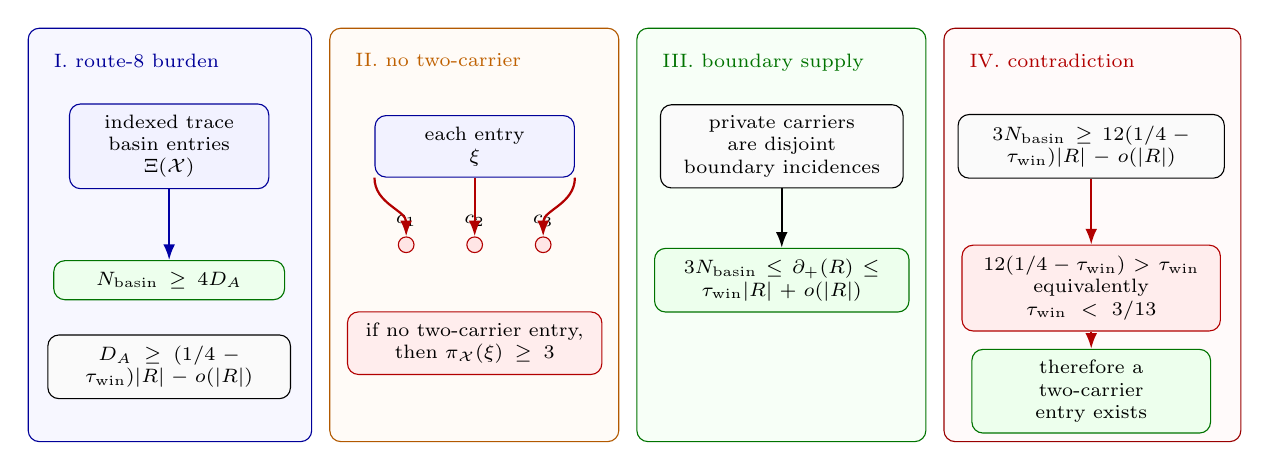
\begin{tikzpicture}[
entry/.style={rectangle,rounded corners,draw=blue!60!black,fill=blue!5,align=center,inner sep=4pt,text width=2.25cm},
carrier/.style={circle,draw=red!70!black,fill=red!10,inner sep=2.0pt},
box/.style={rectangle,rounded corners,draw,fill=black!2,align=center,inner sep=4pt,text width=2.65cm},
good/.style={rectangle,rounded corners,draw=green!45!black,fill=green!7,align=center,inner sep=4pt,text width=2.65cm},
bad/.style={rectangle,rounded corners,draw=red!70!black,fill=red!7,align=center,inner sep=4pt,text width=2.65cm},
arr/.style={-{Latex[length=2mm]},thick},
every node/.style={font=\scriptsize}
]
\draw[rounded corners,fill=blue!3,draw=blue!60!black] (-7.65,-2.80) rectangle (-4.05,2.45);
\draw[rounded corners,fill=orange!3,draw=orange!70!black] (-3.82,-2.80) rectangle (-0.15,2.45);
\draw[rounded corners,fill=green!3,draw=green!45!black] (0.08,-2.80) rectangle (3.75,2.45);
\draw[rounded corners,fill=red!2,draw=red!60!black] (3.98,-2.80) rectangle (7.75,2.45);
\node[anchor=north west,blue!60!black] at (-7.45,2.25) {I. route-8 burden};
\node[anchor=north west,orange!75!black] at (-3.62,2.25) {II. no two-carrier};
\node[anchor=north west,green!45!black] at (0.28,2.25) {III. boundary supply};
\node[anchor=north west,red!70!black] at (4.18,2.25) {IV. contradiction};

\node[entry] (basins) at (-5.86,0.95) {indexed trace\\basin entries\\\(\Xi(\mathcal X)\)};
\node[good,text width=2.65cm] (burden) at (-5.86,-0.75) {\(N_{\rm basin}\ge4D_A\)};
\draw[arr,blue!65!black] (basins)--(burden);
\node[box,text width=2.80cm] at (-5.86,-1.85) {\(D_A\ge(1/4-\tau_{\rm win})|R|-o(|R|)\)};

\node[entry] (xi) at (-1.98,0.95) {each entry\\\(\xi\)};
\node[carrier,label=above:$c_1$] (c1) at (-2.85,-0.30) {};
\node[carrier,label=above:$c_2$] (c2) at (-1.98,-0.30) {};
\node[carrier,label=above:$c_3$] (c3) at (-1.11,-0.30) {};
\draw[arr,red!70!black] (xi.south west) to[out=-90,in=90] (c1.north);
\draw[arr,red!70!black] (xi.south) -- (c2.north);
\draw[arr,red!70!black] (xi.south east) to[out=-90,in=90] (c3.north);
\node[bad,text width=2.95cm] at (-1.98,-1.55) {if no two-carrier entry,\\then \(\pi_{\mathcal X}(\xi)\ge3\)};

\node[box,text width=2.80cm] (priv) at (1.92,0.95) {private carriers\\are disjoint\\boundary incidences};
\node[good,text width=2.95cm] (upper) at (1.92,-0.75) {\(3N_{\rm basin}\le\defp(R)\le\tau_{\rm win}|R|+o(|R|)\)};
\draw[arr] (priv)--(upper);

\node[box,text width=3.10cm] (lower) at (5.85,0.95) {\(3N_{\rm basin}\ge12(1/4-\tau_{\rm win})|R|-o(|R|)\)};
\node[bad,text width=3.00cm] (contra) at (5.85,-0.85) {\(12(1/4-\tau_{\rm win})>\tau_{\rm win}\)\\equivalently\\\(\tau_{\rm win}<3/13\)};
\draw[arr,red!70!black] (lower)--(contra);
\node[good,text width=2.75cm] (exists) at (5.85,-2.16) {therefore a\\two-carrier entry exists};
\draw[arr,red!70!black] (contra)--(exists);
\end{tikzpicture}%
}
\caption[Visual proof of the route-8 carrier-reduction squeeze]{Visual proof of the route-8 carrier-reduction squeeze.  Panel I records the lower side: a route-8 Type A collection \(\mathcal X\) carrying the large-budget deficit has \(N_{\rm basin}(\mathcal X)\ge4D_A(\mathcal X)\), and \(D_A\) is linear in \((1/4-\tau_{\rm win})|R|\).  Panel II shows the negation of the conclusion: if no indexed entry is two-carrier, then every entry has at least three private essential carriers.  Panel III records the upper side: private essential carriers are disjoint boundary incidences of the canonical supports, so \(3N_{\rm basin}(\mathcal X)\le\defp(R)\le\tau_{\rm win}|R|+o(|R|)\).  Panel IV combines the lower and upper bounds; since \(12(1/4-\tau_{\rm win})>\tau_{\rm win}\), equivalently \(\tau_{\rm win}<3/13\), the no-two-carrier alternative is impossible.}
\label{fig:typeA-route8-carrier-reduction-squeeze}
\end{figure}

\begin{definition}[Terminal two-carrier route-8 obstruction]\label[definition]{def:typeA-terminal-two-carrier}
A \emph{terminal two-carrier route-8 obstruction} is a pair
\[
(\mathfrak E,\xi),
\qquad
\xi=(X,w,u,B_u)\in\mathfrak E,
\]
where \(\mathfrak E\) is the frozen tagged entry family of the current branch,
with the following entry-level properties.
\begin{enumerate}[label=(T\arabic*), leftmargin=2.2em, start=2]
\item The entry \(\xi\) is a true route-8 residual entry in the sense of
\cref{def:typeA-true-route8-residual}: exits (1)--(7) of
\cref{def:typeA-saturated-exits} are absent at its saturated receiver, and
\(B_u\) is target-complete-minimal.
\item The canonical carrier core is nontrivial:
\[
\alpha_{\mathfrak E}(\xi)=|\mathcal C_{\rm ess}(\xi)|\ge2 .
\]
\item The entry is two-carrier in the private-carrier sense:
\[
\pi_{\mathfrak E}(\xi)\le2 .
\]
\item For every \(c\in\mathcal C_{\rm ess}(\xi)\), the \(c\)-deletion witness
of \cref{lem:typeA-essential-deletion-witness} is part of the obstruction data,
with its witnessing target event, declared support, and carrier support recorded
as in \cref{lem:typeA-deletion-witness-declared}.
\end{enumerate}
The definition allows essential carriers of \(\xi\) that are also essential for
other tagged entries.  The large-budget argument is used only to produce such
an entry; it is not a field of the terminal package and is not used by the
no-go theorem.  The package is not restricted to the special case
\(|\mathcal C_{\rm ess}(\xi)|=2\).
\end{definition}

\begin{theorem}[Two-carrier route-8 no-go]\label[theorem]{thm:typeA-two-carrier-nogo}
There is no terminal two-carrier route-8 obstruction in the sense of
\cref{def:typeA-terminal-two-carrier}.
\end{theorem}

\begin{proof}
Suppose that \((\mathfrak E,\xi)\) is a terminal two-carrier route-8
obstruction, and write
\[
\xi=(X,w,u,B_u),
\qquad
\mathcal C=\mathcal C_{\rm ess}(\xi).
\]
By condition (T3) in \cref{def:typeA-terminal-two-carrier}, the set
\(\mathcal C\) has at least two elements; choose \(c\in\mathcal C\).
Condition (T4) says that \(\xi\) is two-carrier, and condition (T5) records the
declared \(c\)-deletion witness supplied by
\cref{lem:typeA-essential-deletion-witness,lem:typeA-deletion-witness-declared}.
By \cref{lem:typeA-two-carrier-deletion-canonical}, the corresponding deletion
quotient lies in \(\mathcal Q_4(w;\mathfrak E)\).  Therefore
\cref{lem:typeA-carrier-deletion-exit} gives exit (4) at the saturated receiver
\(w\).

Condition (T2) says that \(\xi\) is a true route-8 residual entry, so exits
(1)--(7) are absent at \(w\).  This contradicts the occurrence of exit (4).
Hence no terminal two-carrier route-8 obstruction exists.
\end{proof}

\begin{figure}[t]
\centering
\resizebox{0.98\textwidth}{!}{%
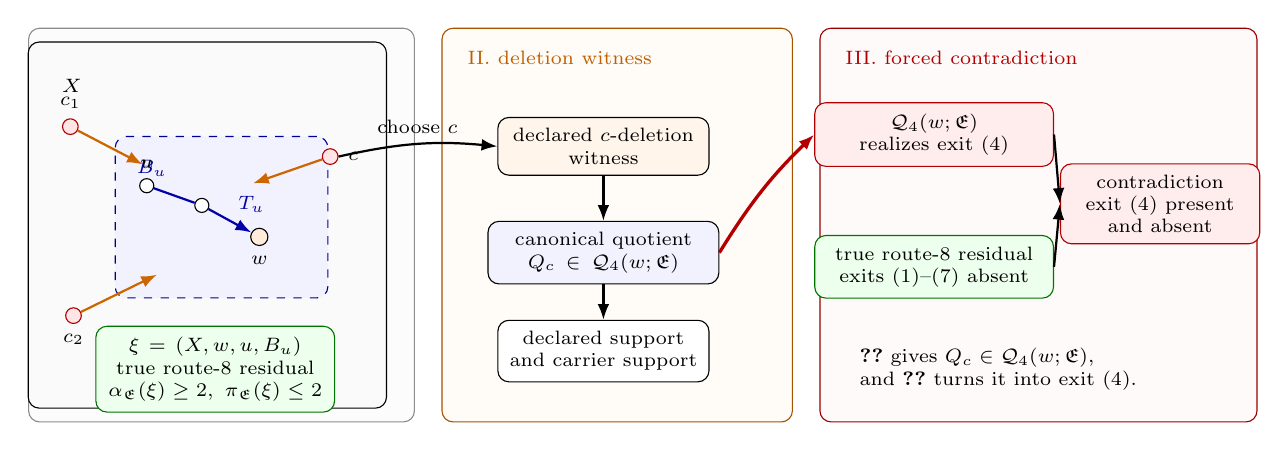
\begin{tikzpicture}[
region/.style={rectangle,rounded corners,draw,fill=black!2,minimum width=4.55cm,minimum height=4.65cm},
basin/.style={rectangle,rounded corners,draw=blue!60!black,dashed,fill=blue!5,minimum width=2.70cm,minimum height=2.05cm},
vtx/.style={circle,draw,fill=white,inner sep=1.8pt},
recv/.style={circle,draw,fill=orange!15,inner sep=2.2pt},
carrier/.style={circle,draw=red!70!black,fill=red!10,inner sep=2.0pt},
witness/.style={rectangle,rounded corners,draw,fill=orange!8,align=center,inner sep=4pt,text width=2.40cm},
quot/.style={rectangle,rounded corners,draw,fill=blue!5,align=center,inner sep=4pt,text width=2.65cm},
exit/.style={rectangle,rounded corners,draw=red!70!black,fill=red!7,align=center,inner sep=4pt,text width=2.75cm},
ok/.style={rectangle,rounded corners,draw=green!45!black,fill=green!7,align=center,inner sep=4pt,text width=2.75cm},
arr/.style={-{Latex[length=2mm]},thick},
bad/.style={-{Latex[length=2mm]},very thick,red!70!black},
every node/.style={font=\scriptsize}
]
\draw[rounded corners,fill=black!1,draw=black!45] (-7.45,-2.45) rectangle (-2.55,2.55);
\draw[rounded corners,fill=orange!3,draw=orange!65!black] (-2.20,-2.45) rectangle (2.25,2.55);
\draw[rounded corners,fill=red!2,draw=red!60!black] (2.60,-2.45) rectangle (8.15,2.55);
\node[anchor=north west] at (-7.25,2.38) {I. terminal route-8 entry};
\node[anchor=north west,orange!75!black] at (-2.00,2.38) {II. deletion witness};
\node[anchor=north west,red!70!black] at (2.80,2.38) {III. forced contradiction};

\node[region] (X) at (-5.18,0.05) {};
\node[anchor=north west] at (-7.15,2.02) {$X$};
\node[basin] (B) at (-5.00,0.15) {};
\node[anchor=north west,blue!60!black] at (-6.20,1.00) {$B_u$};
\node[vtx,label=above:$u$] (u) at (-5.95,0.55) {};
\node[vtx] (a) at (-5.25,0.30) {};
\node[recv,label=below:$w$] (w) at (-4.52,-0.10) {};
\draw[arr,blue!65!black] (u)--(a)--node[above right=-1pt] {$T_u$} (w);
\node[carrier,label=above:$c_1$] (c1) at (-6.92,1.30) {};
\node[carrier,label=below:$c_2$] (c2) at (-6.88,-1.10) {};
\node[carrier,label=right:$c$] (c3) at (-3.62,0.92) {};
\draw[arr,orange!80!black] (c1)--(-6.00,0.82);
\draw[arr,orange!80!black] (c2)--(-5.82,-0.58);
\draw[arr,orange!80!black] (c3)--(-4.60,0.58);
\node[ok] at (-5.08,-1.78) {\(\xi=(X,w,u,B_u)\)\\true route-8 residual\\\(\alpha_{\mathfrak E}(\xi)\ge2,\ \pi_{\mathfrak E}(\xi)\le2\)};

\node[witness] (wit) at (-0.15,1.05) {declared \(c\)-deletion\\witness};
\node[quot] (q) at (-0.15,-0.30) {canonical quotient\\\(Q_c\in\mathcal Q_4(w;\mathfrak E)\)};
\node[witness,fill=white] (supp) at (-0.15,-1.55) {declared support\\and carrier support};
\draw[arr] (wit)--(q);
\draw[arr] (q)--(supp);
\draw[arr] (c3.east) to[bend left=9] node[above] {choose \(c\)} (wit.west);

\node[exit] (forced) at (4.05,1.20) {\(\mathcal Q_4(w;\mathfrak E)\)\\realizes exit (4)};
\node[ok] (absent) at (4.05,-0.48) {true route-8 residual\\exits (1)--(7) absent};
\node[exit,text width=2.25cm,minimum height=0.95cm] (contr) at (6.92,0.32) {contradiction\\exit (4) present and absent};
\draw[bad] (q.east) to[bend left=7] (forced.west);
\draw[arr] (forced.east)--(contr.west);
\draw[arr] (absent.east)--(contr.west);
\node[anchor=west,align=left,text width=4.25cm] at (2.98,-1.78) {\cref{lem:typeA-two-carrier-deletion-canonical} gives \(Q_c\in\mathcal Q_4(w;\mathfrak E)\),\\and \cref{lem:typeA-carrier-deletion-exit} turns it into exit (4).};
\end{tikzpicture}%
}
\caption[Visual proof of the terminal two-carrier route-8 no-go]{Visual proof of the terminal two-carrier route-8 no-go.  Panel I shows a terminal entry \(\xi=(X,w,u,B_u)\) in the frozen tagged family \(\mathfrak E\).  The grey rectangle is the Type A support \(X\), the blue dashed region is the target-complete-minimal basin \(B_u\), the orange vertex is the saturated receiver \(w\), and the red boundary nodes are essential carrier incidences.  The displayed terminal data are \(\alpha_{\mathfrak E}(\xi)\ge2\), \(\pi_{\mathfrak E}(\xi)\le2\), and true route-8 residuality.  Panel II isolates one essential carrier \(c\).  Its declared deletion witness has declared support and carrier support, and the two-carrier deletion lemma places the corresponding quotient in the canonical exit-(4) family \(\mathcal Q_4(w;\mathfrak E)\).  Panel III records the contradiction: the carrier-deletion exit lemma realizes exit (4) at \(w\), while true route-8 residuality says that exits (1)--(7), including exit (4), are absent.  Thus the terminal two-carrier obstruction of \cref{def:typeA-terminal-two-carrier} cannot occur.}
\label{fig:typeA-terminal-route8-nogo-gadget}
\end{figure}

\begin{proposition}[Route-8 closure]\label[proposition]{prop:typeA-route8-closure-from-nogo}
No route-8 Type A collection carries the large-budget Type A deficit.
\end{proposition}

\begin{proof}
Let \(\mathcal X\) be a route-8 Type A collection carrying the large-budget
Type A deficit, and freeze \(\mathfrak E=\Xi(\mathcal X)\).  By
\cref{prop:typeA-route8-carrier-reduction}, \(\mathcal X\)
contains an indexed two-carrier entry
\[
\xi=(X,w,u,B_u)
\]
with \(\pi_{\mathfrak E}(\xi)\le2\).  Since the collection survives only
through route 8, \(\xi\) is a true route-8 residual entry in the sense of
\cref{def:typeA-true-route8-residual}; in particular, exits (1)--(7) are
absent.  By
\cref{lem:typeA-one-terminal-collapse}, every indexed entry in a true route-8
residual has at least two essential carriers, so
\[
\alpha_{\mathfrak E}(\xi)\ge2 .
\]
For each essential carrier,
\cref{lem:typeA-essential-deletion-witness,lem:typeA-deletion-witness-declared}
supplies the required declared deletion witness.  Therefore
\((\mathfrak E,\xi)\) is a terminal two-carrier route-8 obstruction,
contradicting \cref{thm:typeA-two-carrier-nogo}.  Hence no such collection
\(\mathcal X\) exists.
\end{proof}

\begin{remark}[Type A route-8 closure]\label[remark]{rem:typeA-two-carrier-closure}
After \cref{prop:typeA-route8-carrier-reduction}, the only Type A route-8
configuration not eliminated by the private-carrier count is a
target-complete-minimal silent trace basin with at least two essential response
carriers and at most two private essential carriers.  The zero- and
one-essential-carrier cases are removed by \cref{lem:typeA-one-terminal-collapse}.
The remaining two-carrier entry is excluded by
\cref{lem:typeA-two-carrier-deletion-canonical,lem:typeA-carrier-deletion-exit,thm:typeA-two-carrier-nogo}: an essential
carrier has a declared deletion witness, and, for the frozen tagged family
\(\mathfrak E\), the two-carrier condition places the corresponding deletion
quotient in the canonical family \(\mathcal Q_4(w;\mathfrak E)\),
and exit (4) is absent in a true route-8 residual.
\end{remark}

\begin{remark}[Admissibility is essential; the bound is not intrinsic]\label[remark]{rem:typeA-step2}
Subcubicity and an empty $3$-core alone do not yield $2.75$: a
$2$-degenerate subcubic graph can have average degree approaching $3$.  The
point of \cref{lem:density-mersenne} is therefore not a bare extremal statement
about isolated subcubic graphs.  It is a discharging statement for
\emph{admissible} supports, where every receiver also carries the contextual
target algebra, the replacement constraints, the window-stub accounting, and
the saturated-exit alternatives of \cref{def:typeA-saturated-exits}.  The raw
receiver thresholds are $4,8,12$, not the discharging capacities.  They mark the
saturated handoff values $H_0,H_1,H_2$ of
\cref{lem:typeA-threshold-algebra}.  Once exits 1--3, 5, and 6 are closed,
exit 4 has peeled its target-defective routed loads, and exit 7 is handed to
Type B by \cref{lem:typeA-saturated-handoff}, the remaining Type A charge
capacities are $3,7,11$ for internal degrees $2,1,0$.  Route 8 is not a
bare finite graph class: by \cref{lem:typeA-route8-burden} it is reduced to
indexed target-complete-minimal silent trace-basin entries with a linear burden
whenever it carries the large-budget charge deficit, and
\cref{prop:typeA-route8-carrier-reduction} reduces that branch further to the
two-carrier residual of \cref{def:typeA-route8-carriers}.  Thus the density bound is
a statement about completable atoms carrying the full target algebra and
replacement constraints, not about isolated subcubic graphs.
\end{remark}

\paragraph{Framework branch table.}
The Type A subsection closes its local residuals by the following framework
table.
\begin{longtable}{L{0.13\textwidth} L{0.19\textwidth} L{0.14\textwidth} L{0.14\textwidth} L{0.17\textwidth} L{0.17\textwidth}}
\FrameworkBranchTableHeader
Direct exits
&
Saturated exits \textup{(1)}--\textup{(3)} occur.
&
A target hit.
&
The Mersenne-return algebra.
&
One local receiver.
&
Closed by \cref{def:typeA-saturated-exits,lem:typeA-exits-discharged}.
\\
\addlinespace
Target defect
&
Exit \textup{(4)} supplies a routed-load witness.
&
One peel token.
&
The exit-\textup{(4)} ledger.
&
Finite descent in the peeling set.
&
\cref{def:typeA-exit4-peeling,lem:typeA-exit4-peeling-charge,lem:typeA-exit4-discharge}.
\\
\addlinespace
Compression or delocalization
&
Exits \textup{(5)} and \textup{(6)} occur.
&
A proper support.
&
Replacement and smearing.
&
The declared support.
&
\cref{lem:typeA-exits-discharged}.
\\
\addlinespace
Type B handoff
&
Exit \textup{(7)} occurs.
&
Decorated fan data.
&
The Type B ledger.
&
One grouped handoff envelope.
&
\cref{lem:typeA-saturated-handoff,lem:typeA-high-degree-handoff}.
\\
\addlinespace
Unsaturated atom
&
Receiver loads remain below the saturated thresholds.
&
\(3/7/11\) discharging capacity.
&
The deficiency budget.
&
The receiver partition.
&
\cref{lem:typeA-unsaturated-discharge,lem:typeA-exclusion}.
\\
\addlinespace
Route 8
&
A silent trace-basin residual remains.
&
Carrier burden.
&
Carrier-deletion witnesses.
&
The terminal two-carrier package.
&
\cref{prop:typeA-route8-closure-from-nogo}.
\\
\bottomrule
\end{longtable}

\subsection{Type B: high-degree fan-safe surplus obstruction}

\begin{definition}[Assigned Type B charge ledger]\label[definition]{def:typeB-assigned-ledger}
Let $X$ be a connected assigned Type B support.  Write $Y_X$ for the counted
remainder core of $X$, and write $H_X$ for the high-degree fan centers whose
surplus units are assigned to $X$ by \cref{def:canonical-decomp}.  Thus
\[
\defp(X)=\defp(Y_X),\qquad |V(X)|=|V(Y_X)|,\qquad
\sigma(X)=\sum_{h\in H_X}(d_G(h)-3).
\]
A high-degree vertex that appears only as boundary context for another support
is not an element of that support's set $H_X$.  If the same ambient vertex lies
in the local drawing of a support and also supplies a surplus unit, it is entered
once in $H_X$ and is not available as a non-center carrier.

For $y\in Y_X$ set
\[
\delta_X^+(y)=\max\{0,3-d_{Y_X}(y)\},
\qquad
\ch_X(y)=\delta_X^+(y)-\frac14 ,
\]
and for $h\in H_X$ set
\[
\ch_X(h)=-(d_G(h)-3)-\frac14 .
\]
The Type B augmented ledger is
\[
\widehat{\Ch}_B(X)
=
\sum_{y\in Y_X}\ch_X(y)+\sum_{h\in H_X}\ch_X(h).
\]
It satisfies the exact accounting identity
\[
\No(X)
=
\widehat{\Ch}_B(X)+\frac14|H_X|.
\tag{B-ledger}
\]
Consequently $\widehat{\Ch}_B(X)\ge0$ implies $\No(X)\ge0$, hence
\[
\defp(X)-\sigma(X)\ge\frac14|V(X)|.
\]
In a fan envelope, a cubic-closed neighbour has $\delta_X^+=0$ and contributes
$-\tfrac14$; a fan neighbour that is not cubic-closed has internal degree at
most $2$ in the assigned envelope and contributes at least $\tfrac34$.

For a grouped decorated Type B envelope support
\(\mathfrak X_{\mathfrak C}^\ast\) of
\cref{def:decorated-typeB-envelope-support}, the same ledger is used with
\(Y_X=Y_{\mathfrak C}^\ast\) and with the component center-token sum
\(\omega(\mathfrak C)\) in place of the canonically assigned surplus units.
The grouped
ledger is never summed separately from the canonical Type A pieces that
generated it; the transfer identity of \cref{lem:decorated-envelope-no-double-count}
is the summation rule.  Hence an external handoff center, including a center
inside a packed \(P_{13}\)-window, can enter the Type B bridge only through its
grouped envelope component.  In the global fan-mass bound, that surplus unit
may also appear once through the ordinary canonical support containing the
center, and this is the only allowed double use.
\end{definition}

Suppose $X$ carries high-degree surplus, and let $h\in H_X$.  By
\cref{lem:deletion-critical}, the vertices of $H_X$ are independent.  Write
\[
d_G(h)=3+t_h.
\]
The surplus at $h$ is $t_h$, and every unordered pair of neighbours
$u,v\in N(h)$ gives a fan path
\[
u-h-v
\]
of length $2$.  If $G-h$ contains a simple $u$--$v$ path of length
\[
2^j-2\in\{2,6,14,30,\ldots\},
\]
then that path, together with the two edges $hu$ and $hv$, is a cycle of length
$(2^j-2)+2=2^j$.  Thus every neighbour pair of $h$ must be fan-return-safe.

For every $h\in H_X$,
\[
N(h)\text{ is a clique in }\Fsafe_h,
\]
because the failure of one of the five fan-safe conditions is, respectively, a
power-of-two cycle, a legal-label contradiction, a target-defective quotient, a
forbidden target-complete compression, or a proper/global delocalization.  Hence
\[
d_G(h)\le\omega(\Fsafe_h).
\]
Also,
\[
d_G(h)\le\rho(A(\Fsafe_h))+1
\]
by the spectral clique bound: if a clique has size $r$, the corresponding
principal submatrix is $J_r-I_r$, whose largest eigenvalue is $r-1$, and
eigenvalue interlacing gives $r-1\le\rho(A(\Fsafe_h))$.  The Type B branch is
the case in which a negative-charge support contains at least one assigned
high-degree fan center.  The fan-safe graph and marked fan data are those of
\cref{def:typeB-fan-safe,def:marked-typeB-fan}; the fan ledger below accounts
for the surplus terms at those centers.

\begin{lemma}[Fan label packing and certificate-closed charge]\label[lemma]{lem:fan-certificate}
In the Type B fan-certificate graph, the $P_{13}$-label projection with
adjacency relation $C_2(S,T)=1$ has clique number at most $8$.  Every clique in
that projection containing a non-singleton label has size at most $7$.
Consequently every certificate-marked Type B fan has $d_G(h)\le8$, and every
certificate-marked Type B fan with
\[
c-\frac{11-k}{4}\le0,
\qquad k=d_G(h),\quad
c=|\{u\in N(h):u\text{ is cubic-closed}\}|,
\]
has nonnegative closed-neighbourhood charge in the augmented ledger of
\cref{def:typeB-assigned-ledger}.  These are the certificate-closed fans of
\cref{def:typeB-multiclosed-residual}.
\end{lemma}

\begin{proof}
Let $D$ be the graph on $\{0,\ldots,12\}$ in which two distinct indices are
adjacent exactly when their difference is $4$ or $12$.  If
$S_1,\ldots,S_m$ are pairwise $C_2$-compatible labels, choose one representative
$r_i\in S_i$ from each label.  The relation $C_2(S_i,S_j)=1$ says precisely
that no cross-difference between $S_i$ and $S_j$ is $0$, $4$, or $12$.  Hence
the representatives $r_1,\ldots,r_m$ are distinct and form an independent set
in $D$.

The graph $D$ is the disjoint union of the component
\[
0-4-8-12-0
\]
and the three paths
\[
1-5-9,\qquad 2-6-10,\qquad 3-7-11 .
\]
Thus
\[
\alpha(D)=2+2+2+2=8,
\]
and every $C_2$-compatible label family has size at most $8$.  In a
certificate-marked fan the labelling $S_h:N(h)\to\labels$ sends the neighbour
set to such a $C_2$-compatible label family.  Since \(C_2(S,S)=0\), the labels
of distinct neighbours are distinct.  Hence
\[
d_G(h)=|N(h)|=|S_h(N(h))|\le8 .
\]

Now suppose the clique contains a non-singleton label $S$.  Every other label
is contained in
\[
A=\{0,\ldots,12\}\setminus N_D[S],
\]
where $N_D[S]$ is the closed $D$-neighbourhood of $S$, because a cross index
equal to an index of $S$ or at distance $4$ or $12$ from it would violate
$C_2$.  Choose two distinct indices $a,b\in S$.  Deleting the closed
$D$-neighbourhood of $\{a,b\}$ reduces the independence number of $D$ by at
least $2$.  If $a$ and $b$ lie in different components of $D$, each deletion
reduces the corresponding component's independence number by at least $1$.  If
they lie in the same component, that component is either a three-vertex path or
the four-cycle above; in either case the closed neighbourhoods of two distinct
vertices leave independence number $0$ in that component, whereas the original
component had independence number $2$.  Since
$N_D[\{a,b\}]\subseteq N_D[S]$, it follows that
\[
\alpha(D[A])\le6.
\]
Representatives of all labels other than $S$ form an independent set in
$D[A]$, so there are at most $6$ of them.  Therefore every clique containing a
non-singleton label has size at most $7$.

For the charge statement, write $k=d_G(h)$ and let $c$ be the number of
cubic-closed neighbours.  The first packing bound gives $k\le8$.  The
certificate-closed condition used below is exactly the nonpositive-deficit
condition
\[
c-\frac{11-k}{4}\le0.
\]
Equivalently, $c\le1$ when $k\le7$, and $c=0$ when $k=8$.  With the augmented
Type B charge of \cref{def:typeB-assigned-ledger}, the center contributes
\[
\ch_X(h)=3-k-\frac14.
\]
In the worst certificate-closed case with $k\le7$, one neighbour is
cubic-closed and contributes $-\tfrac14$, while the remaining $k-1$ neighbours
contribute at least $\tfrac34$ each.  Therefore
\[
\ch_X(h)+\sum_{u\in N(h)}\ch_X(u)
\ge
\left(3-k-\frac14\right)-\frac14+\frac34(k-1)
=\frac{7-k}{4}\ge0 .
\]
If $k=8$, certificate-closed means $c=0$, so all eight neighbours contribute at
least $\tfrac34$, and
\[
\ch_X(h)+\sum_{u\in N(h)}\ch_X(u)
\ge
\left(3-8-\frac14\right)+8\cdot\frac34
=\frac34>0 .
\]
Thus every certificate-closed marked fan has nonnegative
closed-neighbourhood charge.
\end{proof}

\begin{remark}[The fan-degree bound is label packing]\label[remark]{rem:fan-finite}
The clique bound $d_G(h)\le\omega(\Fsafe_h)$ is an explicit structural
consequence of the label algebra, not a free parameter.  Two neighbours
attaching to a common $P_{13}$ window with labels $S,T$ are fan-return-safe
through that window exactly when $C_2(S,T)=1$: the wedge $u-h-v$ is the
length-two outside path, closing the window into a cycle of length
$4+|i-j|\notin\Pow$.  Since $C_2(S,S)=0$, distinct neighbours carry distinct
labels.  \Cref{lem:fan-certificate} proves that every pairwise
$C_2$-compatible set has size at most $8$, and that every such set containing a
non-singleton label has size at most $7$.  The spectral inequality
$d_G(h)\le\rho(A(\Fsafe_h))+1$ is a secondary quantitative form of this same
packing constraint.  A reader who treats the fan as a bare subcubic graph,
ignoring this label algebra, will not see the bound---just as ignoring
admissibility hides the Type A bound (\cref{rem:local-reading}).
\end{remark}

\begin{definition}[Type B window-incidence profile]\label[definition]{def:typeB-window-incidence-profile}
Let $W$ be the union of the fixed maximal packed induced $P_{13}$ windows.  A
Type B fan-window profile records the assigned fan neighbours that lie in the
remainder side of a decorated envelope; thus each such neighbour lies in
$R=G-W$.  A
\emph{window incidence} of a cubic-closed neighbour $u$ is a triple
\[
(u,P,i)
\]
where $u\notin W$, $P=p_0\cdots p_{12}$ is a packed window, and
$up_i\in E(G)$.  A Type B fan-window profile is \emph{fully window-supported}
when every
cubic-closed neighbour has both non-$h$ neighbours in $W$.  It is
\emph{same-window supported} at $u$ when the two non-$h$ neighbours of $u$ lie
in one packed window.

A \emph{non-window fan incidence} of a cubic-closed neighbour $u$ is an edge
$uz$ with $z\notin W\cup\{h\}$.  A cubic-closed neighbour is
\emph{window-supported}, \emph{mixed-supported}, or \emph{internal-supported}
according as it has two, one, or zero window incidences among its two
non-$h$ incidences.  Thus a mixed-supported neighbour has one window incidence
and one non-window fan incidence, while an internal-supported neighbour has two
non-window fan incidences.

For a surplus port \(p=(h,x)\) whose port vertex \(x\) is recorded on the
remainder side of the fan-window profile, the neighbour \(x\in N(h)\) is
treated as a cubic-closed fan neighbour once the two non-\(h\) incidences
\(xa_p\) and \(xb_p\) are assigned to the fan envelope.  Its support type is
read from the positions of \(a_p\) and \(b_p\): it is window-supported,
mixed-supported, or internal-supported according as two, one, or neither of
those endpoints lies in \(W\).  This convention does not depend on whether
\(a_pb_p\) is an edge of \(G\).
\end{definition}

\begin{definition}[Fan-closed surplus port]\label[definition]{def:fan-closed-port}
Let \(h\) be a high-degree fan center, let \(p=(h,x)\) be a surplus port at
\(h\), and write
\[
N_G(x)=\{h,a_p,b_p\}.
\]
In an assigned Type B fan-window profile \(\mathfrak F_h\), the port \(p\) is
\emph{fan-closed} if the following three conditions hold.
\begin{enumerate}[label=(\alph*), leftmargin=2.2em]
\item The port vertex \(x\) is recorded as a remainder-side fan neighbour of
\(h\).
\item The two non-\(h\) incidences \(xa_p\) and \(xb_p\) are assigned to the fan
envelope of \(\mathfrak F_h\).
\item Each assigned incidence is recorded as either a window incidence or a
non-window fan incidence in the sense of
\cref{def:typeB-window-incidence-profile}.
\end{enumerate}
Thus a fan-closed port contributes one cubic-closed neighbour to the count
\(c(\mathfrak F_h)\) of \cref{def:typeB-multiclosed-residual}.  A fan-closed
port may be triangular, when \(a_pb_p\in E(G)\), or open, when
\(a_pb_p\notin E(G)\).
\end{definition}

\begin{lemma}[Fan-compatible open pairs give fan-closed local data]\label[lemma]{lem:compatible-pair-fan-closure}
Let \(h\) be a high center, and let \(p=(h,x)\) and \(q=(h,y)\) be
fan-compatible open ports at \(h\).  In any assigned Type B fan-window profile
that records \(x\) and \(y\) as remainder-side fan neighbours of \(h\) and
assigns the four incidences
\[
xa_p,\quad xb_p,\quad ya_q,\quad yb_q
\]
to the fan envelope, the ports \(p\) and \(q\) are two distinct fan-closed
ports.  Moreover, these four incidences are pairwise distinct as local
incidence carriers.
\end{lemma}

\begin{proof}
The ports are distinct, so \(x\ne y\).  Since both ports have center \(h\), both
\(x\) and \(y\) lie in \(N_G(h)\); by
\cref{lem:heavy-neighbourhood-normal-form}, they are cubic.  Hence
\[
N_G(x)=\{h,a_p,b_p\},\qquad N_G(y)=\{h,a_q,b_q\}.
\]
The hypotheses of the assigned profile are exactly the three conditions in
\cref{def:fan-closed-port} for \(p\) and for \(q\).  Thus both ports are
fan-closed.

It remains to check that the four displayed incidences are locally distinct.
The two incidences at \(x\) are distinct because \(a_p\ne b_p\), and the two
incidences at \(y\) are distinct because \(a_q\ne b_q\).  No incidence incident
with \(x\) can equal an incidence incident with \(y\), since \(x\ne y\).
\Cref{def:fan-compatible-open-ports} gives \(x\notin s(q)\),
\(y\notin s(p)\), and \(s(p)\cap s(q)=\varnothing\).  Therefore no endpoint of
one displayed incidence can equal the endpoint of another displayed incidence
except at its own port vertex, and the four incidences are pairwise distinct as
local carriers.

\end{proof}

\begin{definition}[Positive-deficit Type B fan-window residual]\label[definition]{def:typeB-multiclosed-residual}
Let $\mathfrak F$ be a marked Type B fan centered at $h$, and write
\[
k=d_G(h),\qquad
c(\mathfrak F)=|\{u\in N(h):u\text{ is cubic-closed in }\mathfrak F\}|.
\]
The \emph{closed-neighbour deficit} of $\mathfrak F$ is
\[
D_B(\mathfrak F)=c(\mathfrak F)-\frac{11-k}{4}.
\]
The fan is \emph{certificate-closed} when
\[
D_B(\mathfrak F)\le0 .
\]
Equivalently, certificate-closed means $c(\mathfrak F)\le1$ for $k\le7$ and
$c(\mathfrak F)=0$ for $k=8$.

A \emph{positive-deficit Type B fan-window residual} is an admissible marked Type
B fan-window profile with $D_B(\mathfrak F)>0$ whose recorded window labels are
pairwise $C_2$-compatible whenever they lie in a common packed window, and whose
fan-window data do not realize a Mersenne return, a target-defective quotient, a
target-complete compression, or a proper/global delocalization.  In this
residual every cubic-closed neighbour is recorded with its two non-$h$
incidences, marked as internal-supported, mixed-supported, or window-supported
according as zero, one, or two of those incidences lie in $W$.  Thus for
$k\le7$ the residual has at least two cubic-closed neighbours; for $k=8$ the
single cubic-closed case is also residual, because its local charge deficit is
$D_B=1/4$.
\end{definition}

\begin{definition}[Hybrid Type B incidence accounting]\label[definition]{def:typeB-hybrid-incidence}
Let $\mathfrak F$ be a positive-deficit Type B fan-window residual.  Write
\[
c_W(\mathfrak F),\quad c_M(\mathfrak F),\quad c_I(\mathfrak F)
\]
for the numbers of window-supported, mixed-supported, and internal-supported
cubic-closed neighbours, respectively.  Thus
\[
c=c_W+c_M+c_I .
\]
The \emph{window-incidence count} and \emph{non-window incidence count} are
\[
I_W(\mathfrak F)=2c_W+c_M,\qquad
I_N(\mathfrak F)=c_M+2c_I .
\]
The \emph{hybrid non-window demand} is
\[
D_N(\mathfrak F)
=
\max\left\{0,\,
D_B(\mathfrak F)-\frac12 I_W(\mathfrak F)
\right\}.
\]
Equivalently,
\[
D_N(\mathfrak F)
=
\max\left\{0,\,
\frac12 I_N(\mathfrak F)-\frac{11-k}{4}
\right\}.
\]
\end{definition}

\begin{figure}[t]
\centering
\resizebox{0.98\textwidth}{!}{%
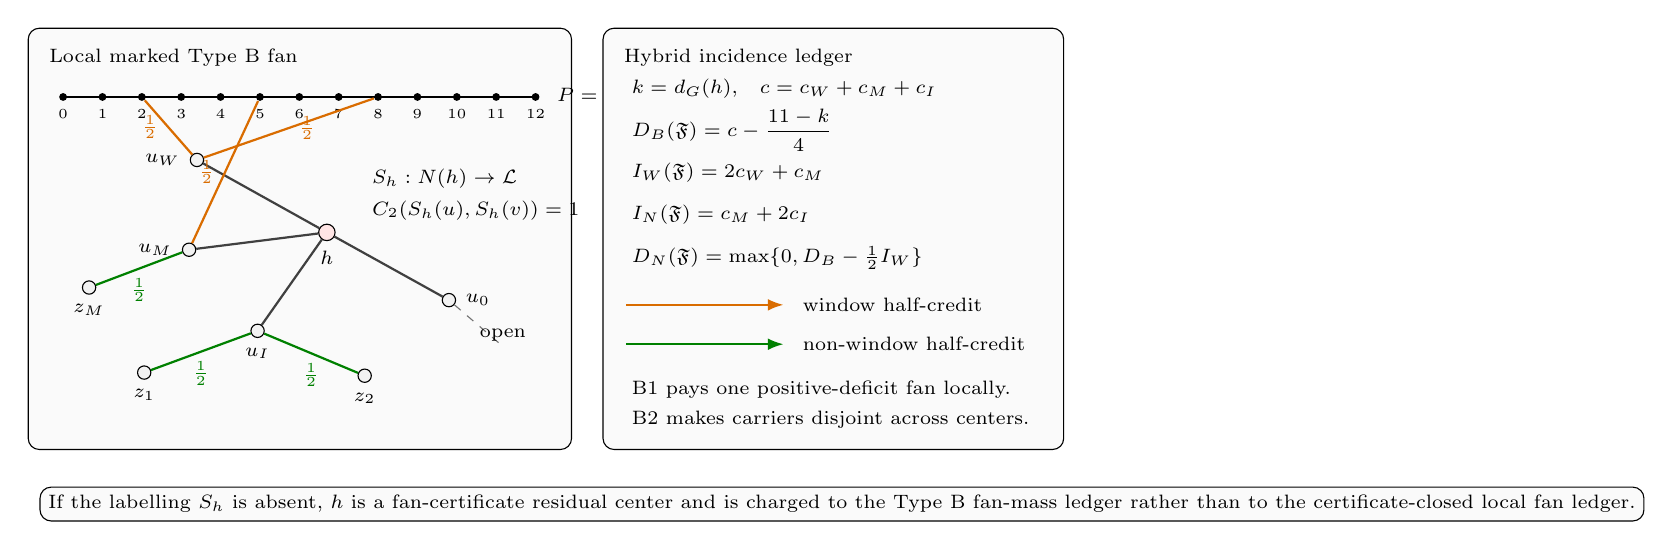
\begin{tikzpicture}[
fanv/.style={circle,draw,fill=black!5,inner sep=1.7pt},
hd/.style={circle,draw,fill=red!10,inner sep=2.1pt},
winv/.style={circle,fill=black,inner sep=1.0pt},
incW/.style={thick,orange!85!black},
incN/.style={thick,green!50!black},
safe/.style={thick,black!75},
box/.style={rectangle,rounded corners,draw,align=left,inner sep=3pt,fill=black!2},
every node/.style={font=\scriptsize}
]
\node[box,anchor=north west,minimum width=6.9cm,minimum height=5.35cm] at (-4.50,2.60) {};
\node[anchor=north west] at (-4.35,2.45) {Local marked Type B fan};
\node[hd,label=below:$h$] (h) at (-0.70,0.00) {};
\node[fanv,label=left:$u_W$] (uW) at (-2.35,0.92) {};
\node[fanv,label=left:$u_M$] (uM) at (-2.45,-0.22) {};
\node[fanv,label=below:$u_I$] (uI) at (-1.58,-1.25) {};
\node[fanv,label=right:$u_0$] (u0) at (0.85,-0.86) {};
\draw[safe] (h)--(uW);
\draw[safe] (h)--(uM);
\draw[safe] (h)--(uI);
\draw[safe] (h)--(u0);
\node[anchor=west] at (-0.25,0.68) {$S_h:N(h)\to\labels$};
\node[anchor=west] at (-0.25,0.28) {$C_2(S_h(u),S_h(v))=1$};

\draw[thick] (-4.05,1.72)--(1.95,1.72);
\foreach \i in {0,...,12} {
  \node[winv] (p\i) at (-4.05+0.50*\i,1.72) {};
  \node[font=\tiny,below=1pt] at (-4.05+0.50*\i,1.72) {$\i$};
}
\node[anchor=west] at (2.10,1.72) {$P=p_0\cdots p_{12}$};

\draw[incW] (uW)--node[left]{$\frac12$}(p2);
\draw[incW] (uW)--node[right]{$\frac12$}(p8);
\draw[incW] (uM)--node[left]{$\frac12$}(p5);
\node[fanv,label=below:$z_M$] (zM) at (-3.72,-0.70) {};
\node[fanv,label=below:$z_1$] (z1) at (-3.02,-1.78) {};
\node[fanv,label=below:$z_2$] (z2) at (-0.22,-1.82) {};
\draw[incN] (uM)--node[below]{$\frac12$}(zM);
\draw[incN] (uI)--node[below]{$\frac12$}(z1);
\draw[incN] (uI)--node[below]{$\frac12$}(z2);
\draw[dashed,black!55] (u0)--(1.55,-1.46);
\node[anchor=west] at (1.12,-1.30) {open};

\node[box,anchor=north west,minimum width=5.85cm,minimum height=5.35cm] at (2.80,2.60) {};
\node[anchor=north west] at (2.95,2.45) {Hybrid incidence ledger};
\node[anchor=west] at (3.05,1.82) {$k=d_G(h)$,\quad $c=c_W+c_M+c_I$};
\node[anchor=west] at (3.05,1.30) {$D_B(\mathfrak F)=c-\dfrac{11-k}{4}$};
\node[anchor=west] at (3.05,0.76) {$I_W(\mathfrak F)=2c_W+c_M$};
\node[anchor=west] at (3.05,0.22) {$I_N(\mathfrak F)=c_M+2c_I$};
\node[anchor=west] at (3.05,-0.32) {$D_N(\mathfrak F)=\max\{0,D_B-\frac12 I_W\}$};
\draw[-{Latex[length=2mm]},thick,orange!85!black] (3.10,-0.92)--(5.10,-0.92);
\node[anchor=west] at (5.22,-0.92) {window half-credit};
\draw[-{Latex[length=2mm]},thick,green!50!black] (3.10,-1.42)--(5.10,-1.42);
\node[anchor=west] at (5.22,-1.42) {non-window half-credit};
\node[anchor=west] at (3.05,-2.00) {B1 pays one positive-deficit fan locally.};
\node[anchor=west] at (3.05,-2.38) {B2 makes carriers disjoint across centers.};

\node[box,anchor=west] at (-4.35,-3.45) {If the labelling $S_h$ is absent, $h$ is a fan-certificate residual center and is charged to the Type B fan-mass ledger rather than to the certificate-closed local fan ledger.};
\end{tikzpicture}%
}
\caption[Visual definition of the Type B fan-window ledger]{Visual definition of the Type B fan-window and hybrid ledger data.  The left panel is the local marked Type B fan, with high-degree center $h$ and neighbours in $N(h)$; the right panel is the hybrid incidence ledger.  The horizontal black path $P=p_0\cdots p_{12}$ is a packed induced $P_{13}$ window, with the displayed indices naming its vertices.  The labelling $S_h:N(h)\to\labels$ assigns fan certificates, and the condition $C_2(S_h(u),S_h(v))=1$ states pairwise fan-safety for distinct neighbours.  The neighbour $u_W$ is window-supported because both of its non-$h$ incidences go to window vertices; $u_M$ is mixed-supported because one incidence goes to the window and one to a non-window vertex $z_M$; $u_I$ is internal-supported because its two non-$h$ incidences go to non-window vertices $z_1,z_2$; and $u_0$ is an open neighbour, so it is not counted as cubic-closed in this local ledger.  Orange edges are window incidences, green edges are non-window incidences, and each displayed $\frac12$ is the half-credit contributed by one such incidence.  In the ledger, $k=d_G(h)$, $c=c_W+c_M+c_I$ counts cubic-closed neighbours by support type, $D_B(\mathfrak F)=c-(11-k)/4$ is the closed-neighbour deficit, $I_W=2c_W+c_M$ is the window-incidence count, $I_N=c_M+2c_I$ is the non-window-incidence count, and $D_N=\max\{0,D_B-\frac12 I_W\}$ is the remaining non-window demand.  B1 denotes the local payment of one positive-deficit fan, while B2 denotes the cross-center disjointness ledger needed to sum those payments globally.  The bottom boxed note records the alternate case: if the labelling $S_h$ is absent, then $h$ is charged as a fan-certificate residual center in the Type B fan-mass ledger.}
\label{fig:typeB-fan-window-ledger-gadget}
\end{figure}

\begin{definition}[Closed fan-window pair]\label[definition]{def:closed-fan-window-pair}
Let $P=p_0p_1\cdots p_{12}$ be a packed induced $P_{13}$ window.  Suppose
$u$ is a cubic-closed neighbour of a Type B fan center $h$ and is same-window
supported at $P$.  Its
\emph{closed label}
\[
S(u)=\{a_u,b_u\}\subseteq\{0,\ldots,12\},\qquad a_u<b_u,
\]
meaning that $u$ is adjacent to $h,p_{a_u},p_{b_u}$ and has no other incident
edge in the assigned fan-window envelope.  For two cubic-closed neighbours
$u,v$ same-window supported at $P$, put $S(v)=\{a_v,b_v\}$ and define
\[
L_h(x,y)=4+|x-y|\qquad (x\in S(u),\ y\in S(v)).
\]
If the four endpoints interlace, say $a_u<a_v<b_u<b_v$ after possibly swapping
$u$ and $v$, define
\[
L_\times(u,v)=4+(a_v-a_u)+(b_v-b_u).
\]
If the endpoints do not interlace, $L_\times(u,v)$ is undefined.
\end{definition}

\begin{definition}[Direct-cycle-free closed pair]\label[definition]{def:direct-cycle-free-closed-pair}
A closed fan-window pair $(u,v)$ is \emph{direct-cycle-free} when all of the
following arithmetic conditions hold:
\begin{enumerate}[label=(\alph*), leftmargin=2.2em]
\item
\[
b_u-a_u,\ b_v-a_v\notin\{2,6\};
\]
\item
\[
|x-y|\notin\{0,4,12\}\qquad (x\in S(u),\ y\in S(v));
\]
\item if $L_\times(u,v)$ is defined, then
\[
L_\times(u,v)\notin\{8,16\}.
\]
\end{enumerate}
\end{definition}

\begin{lemma}[Direct fan-window cycle eliminations]\label[lemma]{lem:typeB-direct-fan-window-cycles}
Let $u,v$ be distinct cubic-closed neighbours of a Type B fan center $h$ that
are same-window supported at the same packed window $P$.  If the closed
fan-window pair $(u,v)$ is not direct-cycle-free and $h\notin V(P)$, then the
envelope contains a power-of-two cycle.  The condition $h\notin V(P)$ holds
for an ordinary remainder-side fan center.  A handoff center lying in a packed
window is handled only through its grouped decorated envelope and is not an
instance of this local lemma.
\end{lemma}

\begin{proof}
Write $S(u)=\{a_u,b_u\}$ and $S(v)=\{a_v,b_v\}$ as in
\cref{def:closed-fan-window-pair}.  If $b_u-a_u\in\{2,6\}$, then
\[
u p_{a_u}\,P\,p_{b_u}u
\]
is a simple cycle of length $(b_u-a_u)+2\in\{4,8\}$, because $u\notin W$ and
$P$ is a simple induced path.  If $b_v-a_v\in\{2,6\}$, then
\[
v p_{a_v}\,P\,p_{b_v}v
\]
is a simple cycle of length $(b_v-a_v)+2\in\{4,8\}$ for the same reason.

If $|x-y|\in\{0,4,12\}$ for some $x\in S(u)$ and $y\in S(v)$, then
\[
u h v p_y\,P\,p_x u
\]
is a simple cycle: the vertices $u$ and $v$ are distinct and lie outside $W$,
whereas the segment $p_yPp_x$ lies inside the packed window.  Its length is
$2+1+|x-y|+1=4+|x-y|\in\{4,8,16\}$.

Finally suppose the endpoints interlace.  After possibly swapping $u$ and $v$,
write
\[
a_u<a_v<b_u<b_v.
\]
The two path segments $p_{a_u}Pp_{a_v}$ and $p_{b_u}Pp_{b_v}$ are internally
vertex-disjoint, and $u,v\notin W$.  Hence
\[
u p_{a_u}\,P\,p_{a_v}v p_{b_v}\,P\,p_{b_u}u
\]
is a simple cycle of length
\[
4+(a_v-a_u)+(b_v-b_u)=L_\times(u,v).
\]
If this length is $8$ or $16$, the cycle is a power-of-two cycle.  These cases
are exactly the negations of the direct-cycle-free conditions.
\end{proof}

\begin{lemma}[Two-window direct cycle eliminations]\label[lemma]{lem:typeB-two-window-cycles}
Let $u,v$ be distinct cubic-closed neighbours of a Type B fan center $h$.
Suppose $u$ and $v$ have incidences to two distinct packed windows
\[
P=p_0\cdots p_{12},\qquad Q=q_0\cdots q_{12},
\]
with
\[
up_i,\ vp_j,\ uq_a,\ vq_b\in E(G).
\]
If
\[
|i-j|+|a-b|\in\{0,4,12\},
\]
then the fan-window envelope contains a power-of-two cycle.
\end{lemma}

\begin{proof}
By the definition of a window incidence, $u$ and $v$ lie outside $W$.  The
packed windows are vertex-disjoint, so the path segments $p_iPp_j$ and
$q_aQq_b$ are vertex-disjoint and avoid $u$ and $v$.  Hence
\[
u p_i\,P\,p_j v q_b\,Q\,q_a u
\]
is a simple cycle.  Its length is
\[
1+|i-j|+1+1+|a-b|+1=4+|i-j|+|a-b|.
\]
If $|i-j|+|a-b|\in\{0,4,12\}$, this length is $4$, $8$, or $16$.
\end{proof}

\begin{lemma}[Positive-deficit fan-window budget]\label[lemma]{lem:typeB-multiclosed-budget}
Let $\mathfrak F$ be an admissible positive-deficit Type B fan-window residual
centered at $h$, with $k=d_G(h)$ and $c=c(\mathfrak F)$.  Then
\[
4\le k\le8,\qquad D_B(\mathfrak F)>0,
\]
and more explicitly either $k\le7$ and $c\ge2$, or $k=8$ and $c\ge1$.
If $k=8$, no cubic-closed neighbour is same-window supported with a
non-singleton label.  For every $k$, every same-window supported cubic-closed
neighbour has internal label gap outside $\{2,6\}$, every same-window closed
fan-window pair in $\mathfrak F$ is direct-cycle-free, and in any assigned Type
B support containing $\mathfrak F$ the closed fan neighbourhood has augmented
charge lower bound
\[
\ch_X(h)+\sum_{u\in N(h)}\ch_X(u)
\ge \frac{11-k}{4}-c .
\]
Equivalently, the remaining Type B charge deficit is exactly
\[
D_B(\mathfrak F)=c-\frac{11-k}{4}>0 .
\]
Assume in addition that $\mathfrak F$ is fully window-supported and contains no
direct cycle of the forms in
\cref{lem:typeB-direct-fan-window-cycles,lem:typeB-two-window-cycles}.  Then its
$c$ cubic-closed neighbours use exactly $2c$ distinct packed-window incidences,
and
\[
D_B(\mathfrak F)\le\frac12\cdot 2c-\frac34 .
\]
\end{lemma}

\begin{proof}
The residual is a marked Type B fan, so its certificate labelling
$S_h:N(h)\to\labels$ is part of the data.  Therefore the fan degree bound gives
$k\le8$ by \cref{lem:fan-certificate}.  If $k=8$, then a same-window supported
cubic-closed neighbour would carry a non-singleton label, and the non-singleton
clique cap in \cref{lem:fan-certificate} would force $k\le7$, a contradiction.
Hence no cubic-closed neighbour of an actual $8$-fan residual is same-window
supported with a non-singleton label.  Since the fan is Type B, $k\ge4$, so
$4\le k\le8$.  The positive-deficit hypothesis is
$D_B(\mathfrak F)>0$, i.e.
\[
c>\frac{11-k}{4}.
\]
As $c$ is integral, this gives $c\ge2$ for $k\le7$ and $c\ge1$ for $k=8$.

If a cubic-closed neighbour $u$ is same-window supported at
$P=p_0\cdots p_{12}$ and has closed label $S(u)=\{a_u,b_u\}$ with
$b_u-a_u\in\{2,6\}$, then
\[
u p_{a_u}\,P\,p_{b_u}u
\]
is a simple cycle of length $4$ or $8$, contradicting admissibility.  If some
same-window closed pair were not direct-cycle-free,
\cref{lem:typeB-direct-fan-window-cycles} would give a power-of-two cycle,
contradicting admissibility.  Hence every single same-window label has gap
outside $\{2,6\}$, and every same-window closed pair is direct-cycle-free.

For the augmented Type B charge, the fan center contributes
\[
\ch_X(h)=(3-k)-\frac14.
\]
Each cubic-closed neighbour contributes $-\tfrac14$, and each of the remaining
$k-c$ neighbours has internal degree at most $2$ in the assigned fan support and
therefore contributes at least $\tfrac34$.  Hence
\[
\ch_X(h)+\sum_{u\in N(h)}\ch_X(u)
\ge
\left(3-k-\frac14\right)-\frac c4+\frac34(k-c)
=\frac{11-k}{4}-c .
\]
Because $D_B(\mathfrak F)>0$, this lower bound is strictly negative, and the
deficit is $D_B(\mathfrak F)=c-\frac{11-k}{4}$.

Now assume $\mathfrak F$ is fully window-supported and contains no direct cycle
of the two displayed forms.  Each cubic-closed neighbour has exactly two
non-$h$ neighbours, both in packed windows, so the number of packed-window
incidences counted with multiplicity is $2c$.  These incidences are distinct.
Indeed, two different closed neighbours cannot use the same packed-window
vertex: if $up_i$ and $vp_i$ were both present, then the fan-cross cycle
\[
u-h-v-p_i-u
\]
has length $4$.  One closed neighbour cannot use the same packed-window vertex
twice because the graph is simple.  Incidences in different packed windows are
distinct because the packing is vertex-disjoint.  Thus the residual uses
exactly $2c$ distinct packed-window incidences.

Since $k\le8$,
\[
\frac{11-k}{4}\ge\frac34.
\]
Therefore
\[
D_B(\mathfrak F)=c-\frac{11-k}{4}\le c-\frac34
=\frac12\cdot 2c-\frac34.
\]
Equivalently, half a unit of reserved credit per distinct packed-window
incidence pays the local Type B deficit with at least three quarters of a unit of
slack.
\end{proof}

\begin{lemma}[Hybrid incidence budget for positive-deficit fans]\label[lemma]{lem:typeB-hybrid-incidence-budget}
Let $\mathfrak F$ be an admissible positive-deficit Type B fan-window residual
centered at $h$.  Suppose that none of the direct-cycle conclusions of
\cref{lem:typeB-direct-fan-window-cycles,lem:typeB-two-window-cycles} occurs.
Then the $2c(\mathfrak F)$ non-$h$ incidences of the cubic-closed neighbours of
$h$ are pairwise disjoint as incidence carriers.  The window incidences supply
half-credit $\frac12 I_W(\mathfrak F)$, and the non-window incidences supply a
disjoint local reserve of size at least
\[
D_N(\mathfrak F)
=
\max\left\{0,\,
D_B(\mathfrak F)-\frac12 I_W(\mathfrak F)
\right\}.
\]
Consequently the hybrid fan entry supplies at least $D_B(\mathfrak F)$.
\end{lemma}

\begin{proof}
Let $u$ and $v$ be distinct cubic-closed neighbours of $h$.  If a non-$h$
neighbour $z$ were incident with both $u$ and $v$, then
\[
u-h-v-z-u
\]
would be a simple $4$-cycle, because $u$ and $v$ are distinct, $z\ne h$, and the
fan neighbours have ambient degree $3$.  This is forbidden by dyadic-safety.
One cubic-closed neighbour cannot use the same non-$h$ endpoint twice, since
$G$ is simple.  Hence the two non-$h$ incidences of all cubic-closed neighbours
are pairwise disjoint as incidence carriers.

The window incidences among them are counted by $I_W(\mathfrak F)$ and the
non-window incidences by $I_N(\mathfrak F)$.  By the local accounting rule in
\cref{def:typeB-hybrid-incidence}, each such incidence carries half-credit;
the window/non-window classification determines which of the two local pools
contains it.  No global carrier choice is used at this point.
Thus the total local incidence capacity is
\[
\frac12 I_W(\mathfrak F)+\frac12 I_N(\mathfrak F)
=
\frac12\cdot2c(\mathfrak F)
=
c(\mathfrak F).
\]
Since
\[
D_B(\mathfrak F)=c(\mathfrak F)-\frac{11-k}{4}
\]
and $k\le8$, this total capacity pays $D_B(\mathfrak F)$ with slack at least
$\frac{11-k}{4}\ge\frac34$.

After the window half-credit has been applied, the remaining demand is
\[
\max\left\{0,\,
D_B(\mathfrak F)-\frac12 I_W(\mathfrak F)
\right\}
=D_N(\mathfrak F).
\]
The available non-window half-credit is
\[
\frac12 I_N(\mathfrak F)
=
c(\mathfrak F)-\frac12 I_W(\mathfrak F)
=
D_B(\mathfrak F)+\frac{11-k}{4}-\frac12 I_W(\mathfrak F),
\]
which is at least $D_N(\mathfrak F)$.  The disjointness proved in the first
paragraph permits these non-window incidence carriers to be chosen disjointly
inside the single fan entry.
\end{proof}

\begin{lemma}[Local hybrid fan entry]\label[lemma]{lem:typeB-hybrid-B1}
Let $\mathfrak F$ be an admissible positive-deficit Type B fan-window residual.
After the direct-cycle, target-defect, compression, and delocalization
alternatives are excluded, the packed-window incidences and the local
internal/mixed incidence reserve form a disjoint local fan entry whose total
capacity is at least $D_B(\mathfrak F)$.
\end{lemma}

\begin{proof}
The excluded target-defect, compression, and delocalization alternatives are
part of the definition of a positive-deficit residual.  The direct-cycle case
has also been excluded.  Therefore
\cref{lem:typeB-hybrid-incidence-budget} supplies the asserted disjoint local
hybrid incidence entry of capacity at least $D_B(\mathfrak F)$.
\end{proof}

\begin{proposition}[Fan-closed ports route to the Type B fan ledger]\label[proposition]{prop:fan-closed-port-typeB-routing}
Let \(h\) be a high-degree fan center of degree \(k\ge4\), and let \(\mathfrak F_h\) be an
admissible Type B fan-window profile that records \(h\) as a fan center.  Suppose
that \(\mathfrak F_h\) contains a set \(\mathcal Q\) of \(r\ge2\) fan-closed
surplus ports at \(h\).  Then the following hold.
\begin{enumerate}[label=(\alph*), leftmargin=2.2em]
\item The ports in \(\mathcal Q\) contribute at least \(r\) cubic-closed
neighbours of \(h\).
\item If the fan at \(h\) is certificate-marked and survives the direct-cycle,
target-defect, compression, and delocalization alternatives in B1, then it is a
positive-deficit Type B fan-window residual with
\[
D_B(\mathfrak F_h)
\ge
r-\frac{11-k}{4}
\ge
\frac{k-3}{4}
>0 .
\]
\item The hybrid B1 ledger supplies local incidence capacity at least
\(D_B(\mathfrak F_h)\).  The paying incidences include the two non-\(h\)
incidences \(xa_p\) and \(xb_p\) of every fan-closed port \(p=(h,x)\in\mathcal Q\),
classified by \cref{def:typeB-window-incidence-profile} as window, mixed, or
non-window incidences according to the locations of \(a_p\) and \(b_p\).
\end{enumerate}
\end{proposition}

\begin{proof}
Let \(p=(h,x)\in\mathcal Q\).  Since \(p\) is fan-closed,
\cref{def:fan-closed-port} records \(x\) as a remainder-side fan neighbour of
\(h\) and assigns the two non-\(h\) incidences \(xa_p\) and \(xb_p\) to the fan
envelope.  By \cref{lem:heavy-neighbourhood-normal-form}, \(x\) is cubic.
Hence \(x\) has internal fan degree \(3\) in the assigned envelope, so it is
cubic-closed in the sense of \cref{def:marked-typeB-fan}.  Distinct ports at
\(h\) have distinct port vertices, and therefore the \(r\) ports in
\(\mathcal Q\) give at least \(r\) cubic-closed neighbours.  This proves (a).

Assume now that the fan is certificate-marked and survives the direct-cycle,
target-defect, compression, and delocalization alternatives in the B1 statement.
Let \(c=c(\mathfrak F_h)\) be the number of cubic-closed neighbours recorded in
the fan envelope.  By (a), \(c\ge r\).  The closed-neighbour deficit is
\[
D_B(\mathfrak F_h)=c-\frac{11-k}{4}.
\]
Therefore
\[
D_B(\mathfrak F_h)
\ge
r-\frac{11-k}{4}
\ge
2-\frac{11-k}{4}
=
\frac{k-3}{4}.
\]
Since \(k\ge4\), the last quantity is positive.  Thus the fan satisfies the
positive-deficit condition of \cref{def:typeB-multiclosed-residual}.  The
profile is admissible by hypothesis; the certificate marking gives the required
\(C_2\)-compatibility of the recorded labels; and the absence of the
direct-cycle, target-defect, compression, and delocalization alternatives is
exactly the surviving B1 hypothesis.  Hence all clauses of
\cref{def:typeB-multiclosed-residual} are satisfied.  This proves (b).

Under the hypotheses of (b), \cref{lem:typeB-hybrid-B1} applies.  It invokes
\cref{lem:typeB-hybrid-incidence-budget}, which gives disjoint local half-credit
on the \(2c\) non-\(h\) incidences of the cubic-closed fan neighbours and pays
at least \(D_B(\mathfrak F_h)\).  For every fan-closed port
\(p=(h,x)\in\mathcal Q\), the two relevant incidences are exactly \(xa_p\) and
\(xb_p\).  \Cref{def:typeB-window-incidence-profile} classifies them according
to whether their non-\(h\) endpoints lie in the packed-window union \(W\).  This
proves (c).

\end{proof}

\begin{corollary}[Fan-compatible open pairs route to the Type B fan ledger]\label[corollary]{cor:compatible-pair-typeB-routing}
Let \(h\) be a high center of degree \(k\ge4\), and let \(p=(h,x)\) and
\(q=(h,y)\) be fan-compatible open ports at \(h\).  In any
admissible Type B fan-window profile that records \(h\) as a fan center,
records \(x\) and \(y\) as remainder-side fan neighbours, and assigns the four
non-\(h\) incidences of \(p\) and \(q\), the fan at \(h\) has two fan-closed
ports.  Consequently it routes through
\cref{prop:fan-closed-port-typeB-routing}.  If the direct-cycle, target-defect,
compression, or delocalization alternative occurs, the branch is already
closed.  If the fan is certificate-marked and those closed alternatives are
absent, then
\[
D_B(\mathfrak F_h)\ge \frac{k-3}{4}>0,
\]
so the B1 ledger pays the local positive-deficit fan.  If the fan is not
certificate-marked, it is passed to the later Type B bridge-residual routing.
\end{corollary}

\begin{proof}
\Cref{lem:compatible-pair-fan-closure} shows that \(p\) and \(q\) are two
distinct fan-closed ports in the assigned profile, with locally distinct
non-\(h\) incidence carriers.  Applying
\cref{prop:fan-closed-port-typeB-routing} with \(\mathcal Q=\{p,q\}\) gives the
displayed deficit bound and the local B1 alternative.
\end{proof}

\begin{corollary}[Triangular ports route to the Type B fan ledger]\label[corollary]{prop:triangular-port-typeB-routing}
Let \(h\) be a heavy center of degree \(k\ge5\), and suppose that the triangular
alternative in \cref{cor:heavy-center-local-dichotomy} holds at \(h\).  Let
\(\mathcal T_h\) be a set of \(k-2\) triangular ports at \(h\).  In any
admissible Type B fan-window profile that records \(h\) as a fan center,
records the port vertices \(x_i\) of \(\mathcal T_h\) as remainder-side fan
neighbours, and assigns the two triangle incidences of every port in
\(\mathcal T_h\), the fan at \(h\) has at least \(k-2\) fan-closed ports.  Hence
it routes through \cref{prop:fan-closed-port-typeB-routing}; in the
certificate-marked B1 survivor,
\[
D_B(\mathfrak F_h)
\ge
(k-2)-\frac{11-k}{4}
=
\frac{5k-19}{4}
>0 .
\]
\end{corollary}

\begin{proof}
For a triangular port \(p_i=(h,x_i)\), the vertex \(x_i\) is a neighbour of
\(h\) and is cubic by \cref{lem:heavy-neighbourhood-normal-form}.  Its two
non-\(h\) neighbours are precisely \(a_i\) and \(b_i\), and both incidences
\(x_i a_i\), \(x_i b_i\) are present in \(G\).  Once those two incidences are
assigned to the fan envelope, \cref{def:fan-closed-port} makes \(p_i\)
fan-closed.  The \(k-2\) ports in \(\mathcal T_h\) have distinct port vertices,
so they contribute at least \(k-2\) fan-closed, hence cubic-closed, neighbours.
Applying \cref{prop:fan-closed-port-typeB-routing} with
\(\mathcal Q=\mathcal T_h\) gives the stated alternatives and the stronger
displayed deficit bound.
\end{proof}

\begin{definition}[Type B ledger carriers]\label[definition]{def:typeB-ledger-carriers}
Let $X$ be a connected assigned Type B support.  A \emph{Type B carrier} in
$X$ is one of the following pieces of support-charge data.
\begin{enumerate}[label=(\alph*), leftmargin=2.2em]
\item a non-center vertex $v\in Y_X$ which is not entered as an assigned
high-degree center, carrying the charge
\[
\ch_X(v)=\delta_X^+(v)-\frac14
\]
from \cref{def:typeB-assigned-ledger};
\item an assigned high-degree center $h\in H_X$, carrying the augmented center
charge
\[
\ch_X(h)=-(d_G(h)-3)-\frac14;
\]
\item a packed-window incidence $(u,P,i)$ of
\cref{def:typeB-window-incidence-profile}, carrying capacity $1/2$ when it is
used as the half-incidence credit of \cref{lem:typeB-multiclosed-budget};
\item a non-window fan incidence $uz$ of
\cref{def:typeB-window-incidence-profile}, carrying capacity $1/2$ when it is
used as the local internal/mixed half-credit of
\cref{lem:typeB-hybrid-incidence-budget};
\item a local internal/mixed reserve block $Q$, contained in the assigned
non-window part of a positive-deficit fan, whose capacity is the sum of the
support charges of its vertices and incidences in the same support-charge
ledger.
\end{enumerate}
The carrier support of a block or incidence is its underlying vertex/incidence
set.  Two carriers are \emph{disjoint} when their underlying supports are
disjoint and neither is part of the ordinary deficiency reserve.  The
\emph{ordinary deficiency reserve} is the unrefined pool of positive-deficiency
units $\delta_X^+(y)$ and packed-window boundary-incidence units counted by
$\defp(X)$ and by the stub supply in \cref{lem:stub-positive}.  A Type B carrier
is disjoint from this reserve precisely when the same vertex or incidence unit
is not also used as one of those unrefined reserve units.
The incidence carriers in (c) and (d) are the global support-ledger
realizations of the two local half-credit pools constructed in
\cref{lem:typeB-hybrid-incidence-budget}; this identification is made only
after the global carrier universe has been defined.
\end{definition}

\begin{definition}[Candidate Type B ledger entries]\label[definition]{def:typeB-candidate-ledger}
Let $X$ be a connected assigned Type B support.  A \emph{Type B demand} is
attached to a marked fan center $h\in H_X$.
\begin{enumerate}[label=(\alph*), leftmargin=2.2em]
\item If the marked fan at $h$ is certificate-closed, a candidate ledger entry is
a set $A_h\subseteq N(h)\setminus H_X$ such that
\[
\ch_X(h)+\sum_{v\in A_h}\ch_X(v)\ge0.
\]
For the finite ledger this condition is checked in quarter units from the
assigned incidences themselves.  If $u\in N(h)$, let

\[
a_h(u)=\bigl|\{z\in N_G(u)\setminus\{h\}:uz\text{ is assigned to the fan
support}\}\bigr|
\quad\text{and}\quad
q_h(u)=11-4\bigl(1+a_h(u)\bigr).
\]

Deletion criticality gives $d_G(u)=3$, so $a_h(u)\in\{0,1,2\}$.  The assigned
fan support may, however, contain decorative or packed-window incidences whose
remote endpoint is outside the counted core $Y_X$.  Put
\[
a_X(u)=\bigl|N_G(u)\cap (Y_X\setminus\{h\})\bigr|,
\qquad
e_h(u)=\bigl|\{z\notin Y_X:uz\text{ is assigned to the fan support}\}\bigr|.
\]
Every core edge is assigned, and the assignment contains only graph edges;
hence $a_h(u)=a_X(u)+e_h(u)$.  Consequently the correct transfer identity is
\[
q_h(u)+4e_h(u)=11-4\bigl(1+a_X(u)\bigr)=4\ch_X(u),
\tag{B-port-transfer}
\]
and in particular $q_h(u)\le4\ch_X(u)$.  Thus $a_h(u)=2$ gives the assigned
cubic-closed weight $q_h(u)=-1$, but it need not say that $u$ has three
neighbours in the counted core: the missing amount is exactly the external
correction $4e_h(u)$.  If $a_h(u)\le1$, then $q_h(u)\ge3$.

The finite certificate-candidate test is

\[
(11-4d_G(h))+\sum_{u\in A_h}q_h(u)\ge0.
\tag{B-candidate-charge}
\]

The test is a lower-bound calculation in the actual induced-core ledger, not
an equality obtained by forgetting external incidences.  Summing
\textup{(B-port-transfer)} transfers it to the displayed augmented-charge
inequality.  For a positive-deficit entry, every packed-window incidence is an
external assigned shoulder and is paid from the corresponding $4e_h(u)$
correction.  A selected non-window half-credit is allowed only when its remote
endpoint $z$ is an ordinary available core vertex: $z\in Y_X\setminus H_X$,
$z$ is adjacent to no assigned center, and $4\ch_X(z)\ge2$.  These ordinary
vertices, the complete fan-neighbour support, and the certificate-selected
vertices are included in the candidate carrier support, so B2 disjointness
prevents their charge from being used twice.
Its carriers are the center $h$ together with the vertices of $A_h$.
\item If the marked fan at $h$ is positive-deficit, a candidate ledger entry is
the fan envelope at $h$, together with all packed-window incidences and enough
non-window fan incidences used by its cubic-closed neighbours to pay the
remaining demand $D_N(\mathfrak F_h)$ of
\cref{def:typeB-hybrid-incidence}.  Each chosen incidence has capacity $1/2$.
By \cref{lem:typeB-hybrid-incidence-budget}, this entry pays
$D_B(\mathfrak F_h)$ with slack at least $(11-k)/4$ before unused incidence
credits are discarded.  Its carriers are the center $h$, the cubic-closed fan
neighbours whose closed-neighbour deficit is being paid, and the chosen
incidence carriers.
\end{enumerate}
A \emph{disjoint refined Type B ledger} is a choice of one candidate entry for
every Type B demand in $X$ such that all chosen carriers are pairwise disjoint.
It is \emph{maximal} when, after the chosen entries are removed, the remaining
core has no high-degree center and no decorated Type B handoff whose center
belongs to $X$.
\end{definition}

\begin{definition}[Minimal Type B overlap obstruction]\label[definition]{def:typeB-overlap-obstruction}
Let $X$ be a connected assigned Type B support.  A \emph{Type B overlap
obstruction} is a pair
\[
\mathcal O=(\mathcal D,\{\mathcal E(d)\}_{d\in\mathcal D})
\]
where $\mathcal D$ is a nonempty finite set of Type B demands in $X$ and
$\mathcal E(d)$ is the set of candidate ledger entries for $d$, such that no
choice of entries
\[
E_d\in\mathcal E(d)\qquad(d\in\mathcal D)
\]
has pairwise disjoint carriers.  The obstruction is \emph{minimal} when every
proper nonempty subfamily of $\mathcal D$ does admit such a disjoint choice.

For each demand, its \emph{declared carrier universe} is the center together
with every vertex or incidence in its finite local item universe, whether or
not reserve conflicts leave a valid candidate entry.  The \emph{overlap
support} $Z(\mathcal O)$ is the union of the declared carrier universes of the
demands in $\mathcal D$, together with the paths or window segments witnessing
the corresponding fan-safe relations.  Thus a demand with an empty valid
candidate set is not erased from the obstruction.  When a connected support is
required below, connected components of this union are considered explicitly;
connectivity is not part of the finite-choice theorem itself.
\end{definition}

\begin{lemma}[Finite choice-or-overlap for a declared Type B family]\label[lemma]{lem:typeB-maximal-completion}
Let $\mathcal D_X$ be a finite duplicate-free family of declared Type B demands
in $X$, and let every demand carry one of the two local entry types of
\cref{def:typeB-candidate-ledger}.  Then exactly the following exhaustive
alternative is available:
\begin{enumerate}[label=(\roman*), leftmargin=2.2em]
\item the whole family $\mathcal D_X$ admits a choice of pairwise disjoint
candidate entries; or
\item a nonempty subfamily is a minimal Type B overlap obstruction.
\end{enumerate}
The conclusion also holds when $\mathcal D_X=\varnothing$, in which case
\textup{(i)} is the vacuous choice.  If $\mathcal D_X$ is the complete family of
centers required by a support assignment, conclusion \textup{(i)} is the full
disjoint-carrier part of B2 for that assignment.
\end{lemma}

\begin{proof}
If the full family has a pairwise-disjoint choice, this is \textup{(i)}.  If it
does not, the full family is a nonempty overlap obstruction: it cannot be empty,
because the empty family has the vacuous choice.  Among the nonempty obstructing
subfamilies choose one of least cardinality.  Every proper nonempty subfamily of
this least obstruction has a disjoint choice, so it is minimal and gives
\textup{(ii)}.  This is a proof-level finite-choice argument; it does not require
enumerating products of candidate sets or the powerset of $\mathcal D_X$.
\end{proof}

For an ordinary vertex support $X$, the complete high-center schedule is
obtained by filtering $V(X)$ at ambient degree at least four.  There is then a
separate exhaustive local-resolution split: either some actual high center has
neither a certificate-closed entry nor a verified positive-B1 entry, or every
high center has one of those entries and hence forms the complete declared
family to which the preceding lemma applies.  This split is distinct from the
later residual-core assertion involving decorated handoffs.

\begin{lemma}[Bridge failure produces a minimal overlap obstruction]\label[lemma]{lem:typeB-bridge-to-overlap}
Let $X$ be a connected assigned Type B support with no fan-certificate residual
center.  If the disjoint-carrier part of the B2 refined support ledger of
\cref{def:typeB-bridge-statements} fails for $X$, then $X$ contains a minimal
Type B overlap obstruction in the sense of \cref{def:typeB-overlap-obstruction}.
\end{lemma}

\begin{proof}
For each high-degree fan center of $X$, form the finite set of candidate ledger
entries in \cref{def:typeB-candidate-ledger}.  The sets are finite because $X$
is finite, every fan neighbour has degree $3$ by \cref{lem:deletion-critical},
and a packed-window incidence uses one of the finitely many labels
$0,\ldots,12$ in a fixed packed window.

Assume that no choice of one candidate entry for every high-degree fan demand
has pairwise disjoint carriers.  Apply
\cref{lem:typeB-maximal-completion} to the complete declared family.  Its first
alternative fails, so the second supplies a least nonempty obstructing
subfamily $\mathcal O$.  Its overlap support is the declared carrier union of
\cref{def:typeB-overlap-obstruction}; no connectivity conclusion is used in
this finite-choice step.

The hybrid B1 fan entry is supplied locally by
\cref{lem:typeB-hybrid-B1}.  Thus a disjoint-carrier failure after B1 is exactly
the overlap obstruction constructed above.  A failure of the maximal residual
core condition is a different alternative: the remaining core still contains a
high-degree center or a decorated Type B handoff, and is routed again through
\cref{lem:typeA-saturated-handoff} and the Type B support assignment rather than
through the overlap-obstruction construction.

Applied to the four-carrier local entry supplied by
\cref{lem:compatible-pair-fan-closure}, this records failure to choose that
entry disjointly from the remaining Type B entries as a minimal Type B overlap
obstruction.
\end{proof}

\begin{corollary}[Global bridge routing for fan-closed local entries]\label[corollary]{cor:fan-closed-global-bridge-routing}
Under the hypotheses of
\cref{prop:fan-closed-port-typeB-routing}, an unmarked fan center is a
fan-certificate residual center.  If the fan is certificate-marked and its
local B1 entry cannot be made disjoint from the other Type B entries in the
assigned support, then that support contains a minimal Type B overlap
obstruction.  These are the two Type B bridge residual alternatives of
\cref{def:typeB-bridge-statements}.
\end{corollary}

\begin{proof}
The first assertion is the fan-certificate residual clause in
\cref{def:marked-typeB-fan}.  In the second case the global disjoint-carrier
clause B2 fails, so \cref{lem:typeB-bridge-to-overlap} supplies the minimal
overlap obstruction.
\end{proof}

\begin{lemma}[Global-to-local reflection of Type B overlap]\label[lemma]{lem:typeB-global-local-reflection}
Let $\mathcal O$ be a minimal Type B overlap obstruction contained in a
connected admissible support $X$.  Then its overlap support $Z=Z(\mathcal O)$
inherits the following global constraints.
\begin{enumerate}[label=(\alph*), leftmargin=2.2em]
\item \emph{Contextual dyadic safety:} no cycle of $G$ meeting $V(Z)$ has
power-of-two length.  Equivalently, no oriented edge in the overlap support has
a Mersenne return through the actual outside context.
\item \emph{High-degree separation:} the high-degree fan centers in
$Z$ are independent, and every neighbour of such a center has ambient degree
$3$.
\item \emph{Window compatibility:} every literal same-window or two-window
datum carried by a demand in $Z$ satisfies the direct-cycle exclusions of
\cref{lem:typeB-direct-fan-window-cycles,lem:typeB-two-window-cycles}.
\item \emph{Replacement obstruction:} every concrete normalized
nonempty-boundary proper atom supported on $Z$ admits no target-complete smaller
representative with the same boundary-degree profile.  Equivalently, any
literal CT3 compression datum for such an atom is contradictory.
\item \emph{Minimal overlap:} every proper connected sub-obstruction of
$\mathcal O$ has a refined disjoint ledger.  Moreover, the demand schedule
cannot be partitioned into two nonempty blocks whose complete declared carrier
universes are disjoint across the partition.
\end{enumerate}
\end{lemma}

\begin{proof}
The support $X$ is admissible by construction of the local analysis.  Hence it
is embedded in the fixed minimal counterexample $G$ and carries all global
constraints listed in \cref{def:admissible,rem:local-reading}.  Since
$Z\subseteq X$, any power-of-two cycle of $G$ meeting $V(Z)$ would also meet
$V(X)$, contradicting contextual dyadic safety of $X$; this proves (a).

For (b), apply \cref{lem:deletion-critical}.  No edge joins two vertices of
ambient degree at least $4$, so the fan centers are independent.  If
$u\in N(h)$ for a high-degree center $h$, then the edge $hu$ has one endpoint
of degree $3$; since $d_G(h)\ge4$, the endpoint forced to have degree $3$ is
$u$.

For (c), if same-window or two-window labels violated the displayed arithmetic
exclusions, the corresponding literal direct-cycle lemma would produce a
power-of-two cycle in $G$, contradicting (a).

For (d), supply the literal normalized boundaried atom, its nonempty boundary
enumeration, and an alleged smaller target-complete representative.  The CT3
gluing theorem derives the whole-graph rank decrease, baseline preservation,
and target transport, and therefore contradicts minimality by
\cref{cor:uncompressible}.  No abstract response flag or unconstructed quotient
is used in this assertion.

Finally, (e) is the minimality clause in
\cref{def:typeB-overlap-obstruction}: every proper nonempty subfamily of
demands admits disjoint candidate entries, hence every proper connected
sub-obstruction has a refined disjoint ledger.  If the full demand family
split into two nonempty blocks with disjoint declared carrier universes, take a
disjoint choice on each proper block and append the choices.  Candidate carrier
supports lie inside their declared universes, so the appended entries are
disjoint across the split, contradicting that $\mathcal O$ is an obstruction.
\end{proof}

\begin{proposition}[Type B bridge residual as a global-to-local obstruction]\label[proposition]{prop:typeB-global-local-bridge}
Every disjoint-carrier Type B bridge residual is represented by a minimal Type B
overlap obstruction satisfying all constraints of
\cref{lem:typeB-global-local-reflection}.  Conversely, if an admissible support
outside the route-8 residual has no fan-certificate residual center and no such
overlap obstruction, then the disjoint-carrier clauses B2(a)--(c) hold there.
Clause B2(d) completes the maximal support assignment.  Together with the
hybrid B1 ledger of \cref{lem:typeB-hybrid-B1}, this gives the quantitative
alternative of \cref{prop:typeB-bridge-reduction}: either the Type B charge is
nonnegative or its negative part is bounded by the assigned surplus.
\end{proposition}

\begin{proof}
The first assertion is \cref{lem:typeB-bridge-to-overlap} followed by
\cref{lem:typeB-global-local-reflection}.  For the converse,
\cref{lem:typeB-hybrid-B1} gives the local B1 entry for every positive-deficit
fan.  The absence of fan-certificate residual centers means that every
high-degree center in the Type B support is certificate-marked.  Since no
multi-demand overlap obstruction is present,
\cref{lem:typeB-maximal-completion} supplies a maximal disjoint refined Type B
ledger.  This proves the disjoint-carrier portion of B2, but does not by itself
pay the deleted-boundary term in \textup{(B-boundary)}.  The additional absence
of an overlap obstruction supplies the full disjoint choice, and B2(d) makes
the support assignment maximal.  The boundary term is then bounded from the
literal size and ambient degree of the selected support, as in
\cref{prop:typeB-bridge-reduction}.  Thus
\[
\max\{0,-\No(X)\}\le
200\sum_{h\in H_X}(d_G(h)-3)
\]
for every connected admissible Type B support outside the saturated and
route-8 residual branches.  When the processed quarter-charge slots admit the
boundary injection, the same proposition gives \(\No(X)\ge0\).
\end{proof}

\begin{figure}[t]
\centering
\resizebox{0.98\textwidth}{!}{%
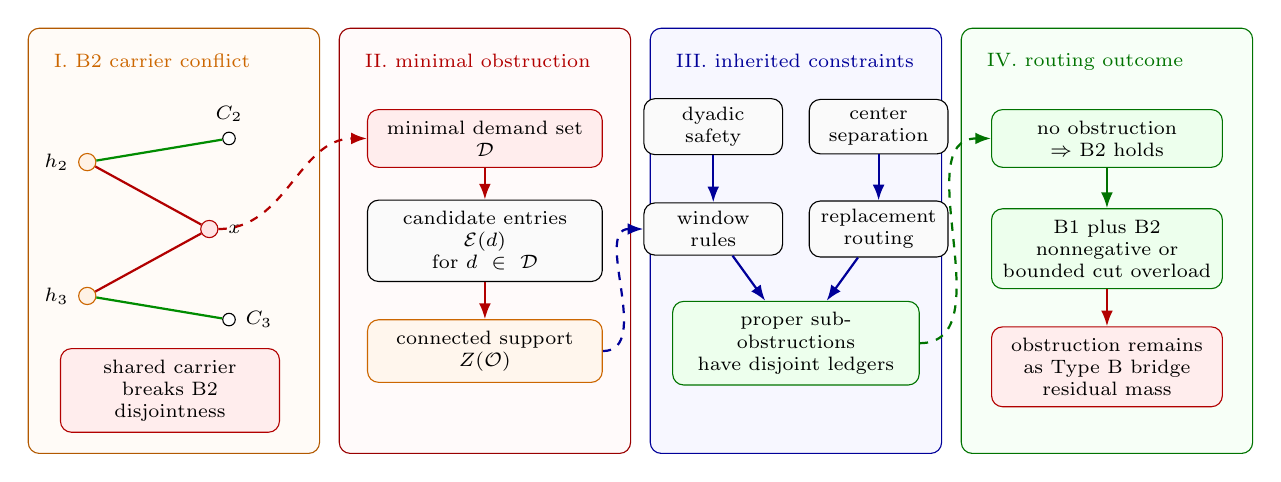
\begin{tikzpicture}[
pt/.style={circle,draw,fill=white,inner sep=1.6pt},
center/.style={circle,draw=orange!80!black,fill=orange!10,inner sep=2.2pt},
carrier/.style={circle,draw=red!70!black,fill=red!10,inner sep=2.2pt},
box/.style={rectangle,rounded corners,draw,fill=black!2,align=center,inner sep=4pt,text width=2.55cm},
good/.style={rectangle,rounded corners,draw=green!45!black,fill=green!7,align=center,inner sep=4pt,text width=2.55cm},
warn/.style={rectangle,rounded corners,draw=orange!80!black,fill=orange!7,align=center,inner sep=4pt,text width=2.55cm},
bad/.style={rectangle,rounded corners,draw=red!70!black,fill=red!7,align=center,inner sep=4pt,text width=2.55cm},
arr/.style={-{Latex[length=2mm]},thick},
dasharr/.style={-{Latex[length=2mm]},thick,dashed},
every node/.style={font=\scriptsize}
]
\draw[rounded corners,fill=orange!3,draw=orange!70!black] (-7.75,-2.85) rectangle (-4.05,2.55);
\draw[rounded corners,fill=red!2,draw=red!60!black] (-3.80,-2.85) rectangle (-0.10,2.55);
\draw[rounded corners,fill=blue!3,draw=blue!60!black] (0.15,-2.85) rectangle (3.85,2.55);
\draw[rounded corners,fill=green!3,draw=green!45!black] (4.10,-2.85) rectangle (7.80,2.55);
\node[anchor=north west,orange!80!black] at (-7.55,2.35) {I. B2 carrier conflict};
\node[anchor=north west,red!70!black] at (-3.60,2.35) {II. minimal obstruction};
\node[anchor=north west,blue!60!black] at (0.35,2.35) {III. inherited constraints};
\node[anchor=north west,green!45!black] at (4.30,2.35) {IV. routing outcome};

\node[center,label=left:\(h_2\)] (h2) at (-7.00,0.85) {};
\node[center,label=left:\(h_3\)] (h3) at (-7.00,-0.85) {};
\node[carrier,label=right:\(x\)] (x) at (-5.45,0.00) {};
\node[pt,label=above:\(C_2\)] (c2a) at (-5.20,1.15) {};
\node[pt,label=right:\(C_3\)] (c3a) at (-5.20,-1.15) {};
\draw[green!55!black,thick] (h2)--(c2a);
\draw[green!55!black,thick] (h3)--(c3a);
\draw[red!70!black,thick] (h2)--(x);
\draw[red!70!black,thick] (h3)--(x);
\node[bad,text width=2.50cm] at (-5.95,-2.05) {shared carrier\\breaks B2\\disjointness};

\node[bad,text width=2.70cm] (demands) at (-1.95,1.15) {minimal demand set\\\(\mathcal D\)};
\node[box,text width=2.70cm] (entries) at (-1.95,-0.15) {candidate entries\\\(\mathcal E(d)\)\\for \(d\in\mathcal D\)};
\node[warn,text width=2.70cm] (support) at (-1.95,-1.55) {connected support\\\(Z(\mathcal O)\)};
\draw[arr,red!70!black] (demands)--(entries);
\draw[arr,red!70!black] (entries)--(support);

\node[box,text width=1.55cm,inner sep=3pt] (safe) at (0.95,1.30) {dyadic\\safety};
\node[box,text width=1.55cm,inner sep=3pt] (sep) at (3.05,1.30) {center\\separation};
\node[box,text width=1.55cm,inner sep=3pt] (win) at (0.95,0.00) {window\\rules};
\node[box,text width=1.55cm,inner sep=3pt] (rep) at (3.05,0.00) {replacement\\routing};
\node[good,text width=2.85cm] (min) at (2.00,-1.45) {proper sub-obstructions\\have disjoint ledgers};
\draw[arr,blue!60!black] (safe)--(win);
\draw[arr,blue!60!black] (sep)--(rep);
\draw[arr,blue!60!black] (win)--(min);
\draw[arr,blue!60!black] (rep)--(min);

\node[good,text width=2.65cm] (b2) at (5.95,1.15) {no obstruction\\\(\Rightarrow\) B2 holds};
\node[good,text width=2.65cm] (close) at (5.95,-0.25) {B1 plus B2\\nonnegative or\\bounded cut overload};
\node[bad,text width=2.65cm] (resid) at (5.95,-1.75) {obstruction remains\\as Type B bridge\\residual mass};
\draw[arr,green!45!black] (b2)--(close);
\draw[arr,red!70!black] (close)--(resid);
\draw[dasharr,red!70!black] (x.east) to[out=0,in=180] (demands.west);
\draw[dasharr,blue!60!black] (support.east) to[out=0,in=180] (win.west);
\draw[dasharr,green!45!black] (min.east) to[out=0,in=180] (b2.west);
\end{tikzpicture}%
}
\caption[Visual proof of the Type B overlap-obstruction routing]{Visual proof of the Type B overlap-obstruction routing.  Panel I shows the disjoint-carrier B2 failure mechanism: two Type B fan demands may have local B1 entries, but their candidate carrier sets can compete for a shared carrier \(x\), so the chosen entries are not disjoint.  Panel II records the finite minimality step of \cref{lem:typeB-bridge-to-overlap}: among all failed demand families, a minimal one gives a Type B overlap obstruction \(\mathcal O=(\mathcal D,\{\mathcal E(d)\})\), and its involved fan centers, carriers, paths, and window segments form the connected overlap support \(Z(\mathcal O)\).  Panel III displays the global constraints inherited by \(Z(\mathcal O)\) in \cref{lem:typeB-global-local-reflection}: contextual dyadic safety, high-degree separation, window compatibility, replacement/delocalization routing, and minimality of the overlap.  Panel IV gives the routing consequence of \cref{prop:typeB-global-local-bridge}: if no such obstruction remains, the disjoint local choice exists.  Its deleted boundary is subsequently bounded by the ambient degree sum of the selected support.}
\label{fig:typeB-overlap-obstruction-routing}
\end{figure}

\begin{definition}[Type B bridge statements]\label[definition]{def:typeB-bridge-statements}
The Type B bridge consists of the local hybrid fan ledger B1 and the global
disjoint support ledger B2.  The local ledger B1 is proved in
\cref{lem:typeB-hybrid-B1}; B2 is the global disjointness and maximal-assignment
statement used in \cref{prop:typeB-bridge-reduction}.  Deleted-boundary
accounting is derived from the selected support and is not a clause of B2.

\emph{(B1) Hybrid fan ledger.}  Every positive-deficit Type B fan-window residual
is one of the following: it contains a direct power-of-two cycle of the forms in
\cref{lem:typeB-direct-fan-window-cycles,lem:typeB-two-window-cycles}; it
realizes a target-defective quotient, a target-complete compression, or a
proper/global delocalization; or its packed-window incidences together with its
local internal/mixed non-window incidences contain a disjoint hybrid fan entry
of capacity at least $D_B(\mathfrak F)$.  The window part contributes
$\frac12 I_W(\mathfrak F)$, and the non-window part contributes the remaining
demand $D_N(\mathfrak F)$ of \cref{def:typeB-hybrid-incidence}.

\emph{(B2) Refined support ledger.}  For any connected assigned Type B support
$X$ with no fan-certificate residual center, the high-degree fan centers of $X$
admit a canonical refined ledger in the sense of
\cref{def:typeB-candidate-ledger}.  Clauses (a)--(c) are the disjoint-carrier
part of B2, and clause (d) is the maximal support-assignment part.
\begin{enumerate}[label=(\alph*), leftmargin=2.2em]
\item Each certificate-closed fan center is assigned a set of incident
non-center vertices whose augmented charge, together with the center charge, is
nonnegative.  The center and the assigned non-center vertices are carriers of
that entry, and no carrier is assigned to two different fan centers.
\item For any maximal canonical family $\mathcal F$ of positive-deficit Type B
residual fans in $X$, each fan center has its hybrid B1 ledger entry: packed
window incidences carry credit $1/2$, and non-window fan incidences carry the
local internal/mixed half-credit needed to pay $D_N$.  These incidence carriers
are disjoint from the ordinary deficiency reserve of
\cref{def:typeB-ledger-carriers}.
\item The certificate-closed entries in (a), the local reserve entries supplied
by B1 for positive-deficit fans, and the half-incidence entries in (b) are
mutually disjoint refinements of the augmented ledger
$\widehat{\Ch}_B(X)$ of \cref{def:typeB-assigned-ledger}.  After the support
assignment is forgotten, this ledger gives $\No(X)$ by the identity
\textup{(B-ledger)}.
\item The ledger is maximal for the Type B support assignment: after the ledger
entries are removed, the remaining core has no high-degree center, no
decorated Type B handoff whose center belongs to \(X\), and no external
decorated handoff that is not already covered by a grouped decorated envelope
processed in the same canonical step.
\end{enumerate}

For a full B2 choice, let \(U\) be the used non-center vertices, put
\(P=U\cup H_X\) and \(Y_0=Y_X\setminus P\), and define
\[
B_\partial=\sum_{v\in Y_0}|N_X(v)\cap P|.
\]
A certificate entry uses at most eight non-center vertices.  A
positive-deficit entry uses at most eight fan neighbours and at most sixteen
remote incidence endpoints.  Hence
\[
 |U|\le24|H_X|,\qquad |P|\le25|H_X|.
\tag{B-support-size}
\]
Every vertex of \(P\) has ambient degree at most eight, and every
\(h\in H_X\) has \(d_G(h)-3\ge1\).  The finite cut bound therefore gives
\[
B_\partial
 \le\sum_{x\in P}d_G(x)
 \le200|H_X|
 \le200\sum_{h\in H_X}(d_G(h)-3).
\tag{B-boundary-size}
\]
The boundary demand consists of \(4B_\partial\) quarter-charge units.  The
canonical finite transfer either injects these units into the processed
quarter-charge slots or returns the strict numerical overload.  This
alternative is a consequence of the two finite cardinalities; it requires no
enumeration of transfer functions.

A \emph{Type B bridge residual} is either:
\begin{enumerate}[label=(\roman*), leftmargin=2.2em]
\item a connected assigned Type B support containing a fan-certificate residual
center of \cref{def:marked-typeB-fan}; or
\item a connected assigned Type B support in which the local B1 entries have
been supplied, the support assignment has been made maximal, and the
disjoint-carrier part of B2 fails; or
\item a grouped decorated Type B envelope support whose envelope ledger cannot
be closed by the center tokens of its core--center incidence component.
\item a connected assigned Type B support for which the disjoint local choices
exist but the boundary demand strictly exceeds the available processed
quarter-charge slots.
\end{enumerate}
In cases (ii) and (iii), the support contains a minimal Type B overlap
obstruction in the sense of \cref{def:typeB-overlap-obstruction}; by
\cref{prop:typeB-global-local-bridge}, that obstruction carries the
global-to-local constraints of \cref{lem:typeB-global-local-reflection}.
Case~(iv) is a separate arithmetic residual.  Its deficit is bounded by
\textup{(B-boundary-size)} and is not identified with an overlap obstruction.
\end{definition}

\begin{corollary}[The local hybrid entry realizes B1]\label[corollary]{cor:typeB-local-entry-is-B1}
The local entry of \cref{lem:typeB-hybrid-B1} is the hybrid fan-ledger
alternative B1 in \cref{def:typeB-bridge-statements}.
\end{corollary}

\begin{proof}
The alternatives excluded in \cref{lem:typeB-hybrid-B1} are exactly the first
two alternatives in B1.  In the remaining case that lemma supplies the
disjoint hybrid entry with window credit $I_W/2$, remaining non-window demand
$D_N$, and total capacity at least $D_B$, which is precisely the third
alternative in the definition of B1.
\end{proof}

\begin{figure}[t]
\centering
\resizebox{0.98\textwidth}{!}{%
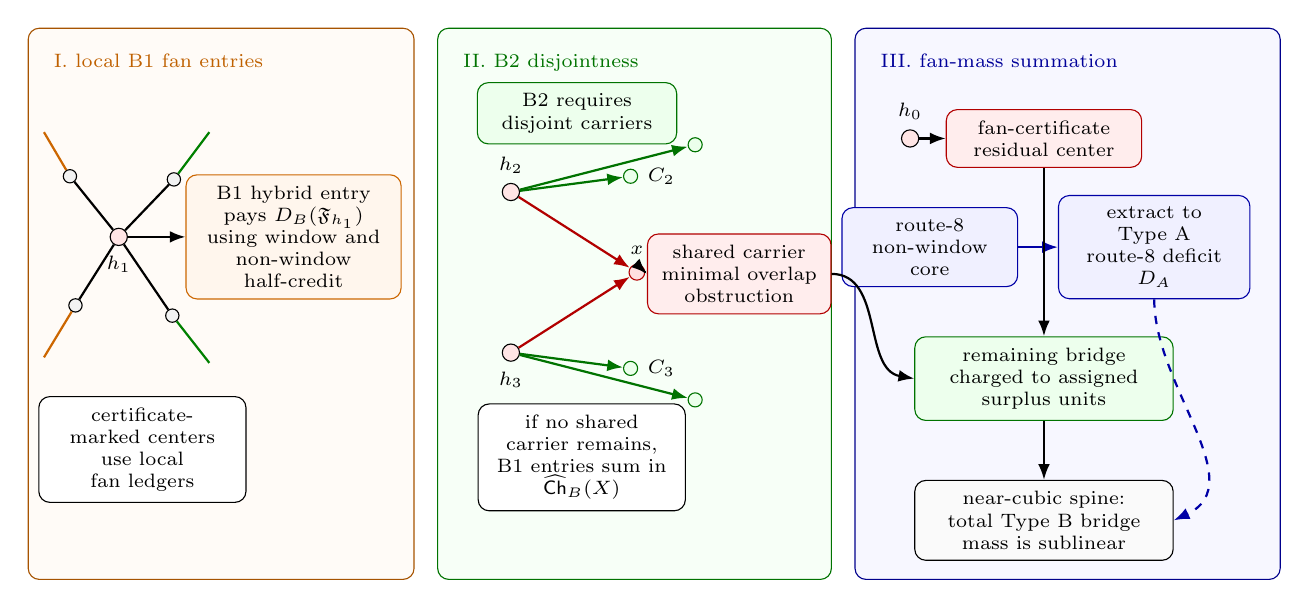
\begin{tikzpicture}[
center/.style={circle,draw,fill=red!10,inner sep=2.2pt},
fanv/.style={circle,draw,fill=black!5,inner sep=1.7pt},
carrier/.style={circle,draw=green!45!black,fill=green!8,inner sep=1.8pt},
over/.style={circle,draw=red!70!black,fill=red!12,inner sep=2.0pt},
box/.style={rectangle,rounded corners,draw,fill=black!2,align=center,inner sep=4pt,text width=2.35cm},
b1/.style={rectangle,rounded corners,draw=orange!80!black,fill=orange!7,align=center,inner sep=4pt,text width=2.45cm},
b2/.style={rectangle,rounded corners,draw=green!45!black,fill=green!7,align=center,inner sep=4pt,text width=2.25cm},
res/.style={rectangle,rounded corners,draw=red!70!black,fill=red!7,align=center,inner sep=4pt,text width=2.35cm},
typea/.style={rectangle,rounded corners,draw=blue!65!black,fill=blue!6,align=center,inner sep=4pt,text width=2.05cm},
arr/.style={-{Latex[length=2mm]},thick},
dasharr/.style={-{Latex[length=2mm]},thick,dashed},
every node/.style={font=\scriptsize}
]
\draw[rounded corners,fill=orange!3,draw=orange!65!black] (-7.55,-3.90) rectangle (-2.65,3.10);
\draw[rounded corners,fill=green!3,draw=green!45!black] (-2.35,-3.90) rectangle (2.65,3.10);
\draw[rounded corners,fill=blue!3,draw=blue!55!black] (2.95,-3.90) rectangle (8.35,3.10);
\node[anchor=north west,orange!75!black] at (-7.35,2.90) {I. local B1 fan entries};
\node[anchor=north west,green!45!black] at (-2.15,2.90) {II. B2 disjointness};
\node[anchor=north west,blue!60!black] at (3.15,2.90) {III. fan-mass summation};

\node[center,label=below:$h_1$] (h1) at (-6.40,0.45) {};
\node[fanv] (a1) at (-7.02,1.22) {};
\node[fanv] (a2) at (-5.70,1.18) {};
\node[fanv] (a3) at (-6.95,-0.42) {};
\node[fanv] (a4) at (-5.72,-0.55) {};
\draw[thick] (h1)--(a1);
\draw[thick] (h1)--(a2);
\draw[thick] (h1)--(a3);
\draw[thick] (h1)--(a4);
\draw[thick,orange!80!black] (a1)--(-7.35,1.78);
\draw[thick,green!50!black] (a2)--(-5.25,1.78);
\draw[thick,orange!80!black] (a3)--(-7.35,-1.08);
\draw[thick,green!50!black] (a4)--(-5.25,-1.15);
\node[b1] (localb1) at (-4.18,0.45) {B1 hybrid entry\\pays \(D_B(\mathfrak F_{h_1})\)\\using window and\\non-window half-credit};
\draw[arr] (h1.east)--(localb1.west);
\node[box,fill=white] at (-6.10,-2.25) {certificate-marked centers\\use local fan ledgers};

\node[center,label=above:$h_2$] (h2) at (-1.42,1.02) {};
\node[center,label=below:$h_3$] (h3) at (-1.42,-1.02) {};
\node[carrier,label=right:$C_2$] (c2a) at (0.10,1.22) {};
\node[carrier] (c2b) at (0.92,1.62) {};
\node[carrier,label=right:$C_3$] (c3a) at (0.10,-1.22) {};
\node[carrier] (c3b) at (0.92,-1.62) {};
\node[over,label=above:$x$] (shared) at (0.18,0.00) {};
\draw[arr,green!45!black] (h2)--(c2a);
\draw[arr,green!45!black] (h2)--(c2b);
\draw[arr,red!70!black] (h2)--(shared);
\draw[arr,green!45!black] (h3)--(c3a);
\draw[arr,green!45!black] (h3)--(c3b);
\draw[arr,red!70!black] (h3)--(shared);
\node[b2] (good) at (-0.58,2.02) {B2 requires\\disjoint carriers};
\node[res,text width=2.05cm] (fail) at (1.48,-0.02) {shared carrier\\minimal overlap\\obstruction};
\draw[arr] (shared.east)--(fail.west);
\node[box,fill=white] at (-0.52,-2.35) {if no shared carrier remains,\\B1 entries sum in\\\(\widehat{\Ch}_B(X)\)};

\node[center,label=above:$h_0$] (h0) at (3.65,1.70) {};
\node[res,text width=2.20cm] (cert) at (5.35,1.70) {fan-certificate\\residual center};
\draw[arr] (h0)--(cert);
\node[typea,text width=1.95cm] (core) at (3.90,0.32) {route-8\\non-window core};
\node[typea,text width=2.15cm] (da) at (6.75,0.32) {extract to Type A\\route-8 deficit\\\(D_A\)};
\draw[arr,blue!65!black] (core)--(da);
\node[b2,text width=3.00cm] (surp) at (5.35,-1.35) {remaining bridge\\charged to assigned\\surplus units};
\node[box,text width=3.00cm] (sum) at (5.35,-3.15) {near-cubic spine:\\total Type B bridge\\mass is sublinear};
\draw[arr] (cert.south)--(surp.north);
\draw[arr] (fail.east) to[out=0,in=170] (surp.west);
\draw[arr] (surp)--(sum);
\draw[dasharr,blue!65!black] (da.south) to[out=-90,in=25] (sum.east);
\end{tikzpicture}%
}
\caption[Visual definition of the Type B bridge and fan-mass summation]{Visual definition of the Type B bridge and fan-mass summation.  Panel I shows the local B1 entry for a positive-deficit Type B fan centered at \(h_1\).  Window incidences and non-window incidences contribute half-credit, and the B1 ledger pays the local deficit \(D_B(\mathfrak F_{h_1})\).  Panel II shows the global B2 disjointness requirement.  Centers \(h_2\) and \(h_3\) may use their own carrier sets \(C_2\) and \(C_3\), but a shared carrier \(x\) is forbidden by B2; a minimal unresolved sharing pattern is the minimal Type B overlap obstruction of \cref{def:typeB-overlap-obstruction}.  Panel III shows the fan-mass summation used for Type B bridge residuals.  A center without the required certificate enters the fan-certificate residual class, a route-8 non-window core is extracted into the Type A route-8 deficit ledger \(D_A\), and the remaining Type B bridge entries are charged to assigned surplus units.  After this extraction, the Type B bridge mass is sublinear in the near-cubic spine, so it cannot carry the linear large-budget deficit.}
\label{fig:typeB-bridge-fanmass-gadget}
\end{figure}

\begin{lemma}[Exact post-B2 charge decomposition]\label[lemma]{lem:typeB-exact-postledger}
Let $X$ be an assigned Type B support and suppose that a full disjoint B2
choice has been made.  Let $U$ be the union of the literal counted-core
vertices whose charges are used by its local entries.  Thus $U\subseteq Y_X$,
$U\cap H_X=\varnothing$, and the per-center subsets forming $U$ are pairwise
disjoint.  Put
\[
Y_0=Y_X\setminus(U\cup H_X).
\]
In quarter units, the selected fan ledger is nonnegative:
\[
0\le
\sum_{h\in H_X}\bigl(-4(d_G(h)-3)-1\bigr)
+\sum_{u\in U}\bigl(4\delta_X^+(u)-1\bigr).
\tag{B-selected}
\]
Moreover the net charge has the exact decomposition
\begin{align*}
4\No(X)
={}&
\left[
\sum_{h\in H_X}\bigl(-4(d_G(h)-3)-1\bigr)
+\sum_{u\in U}\bigl(4\delta_X^+(u)-1\bigr)
\right]\\
&+\left[
\sum_{h\in H_X}\bigl(4\delta_X^+(h)-1\bigr)+|H_X|
\right]
+\sum_{v\in Y_0}\bigl(4\delta_X^+(v)-1\bigr).
\tag{B-postledger}
\end{align*}
The second bracket equals
$4\sum_{h\in H_X}\delta_X^+(h)$ and is therefore nonnegative.  Consequently
either $\No(X)\ge0$, or the literal remaining core has negative charge:
\[
\sum_{v\in Y_0}\bigl(4\delta_X^+(v)-1\bigr)<0.
\tag{B-to-A}
\]
\end{lemma}

\begin{proof}
For a certificate entry, \textup{(B-port-transfer)} bounds every selected
candidate weight by the actual charge of its selected core vertex.  For a
positive-deficit entry, the external-shoulder correction pays the window
credit, and each selected non-window half-credit is bounded by the charge of
its ordinary available remote endpoint.  Candidate carrier support contains
all these vertices and every fan neighbour whose charge occurs in the local
calculation.  B2 therefore makes the corresponding subsets pairwise disjoint,
and summing the local nonnegative balances gives \textup{(B-selected)}.

The sets $U$, $H_X$, and $Y_0$ are disjoint and partition $Y_X$.  Split the
ordinary core-charge sum over this partition, add the augmented center sum,
and then use the exact identity
\[
4\No(X)=4\widehat{\Ch}_B(X)+|H_X|.
\]
This gives \textup{(B-postledger)} by rearrangement.  The asserted form of its
second bracket is pointwise, since
$(4\delta_X^+(h)-1)+1=4\delta_X^+(h)$.  If the final sum is nonnegative, all
three terms on the right of \textup{(B-postledger)} are nonnegative; otherwise
\textup{(B-to-A)} holds.
\end{proof}

\begin{lemma}[Post-ledger Type A boundary identity]\label[lemma]{lem:typeB-postledger-core-hygiene}
Let \(X\) be a Type B support and let \(P=U\cup H_X\) be the vertices removed
by a disjoint local ledger.  Put \(Y_0=Y_X\setminus P\), and let \(Z\) be a
connected component of the graph induced by \(Y_0\).  Every vertex of \(Y_0\)
has ambient degree \(3\).  For \(v\in Z\), let
\[
 b_Z(v)=|N_X(v)\cap P|
\]
be the number of original-core incidences deleted at \(v\).  Then
\[
 d_Z(v)=d_X(v)-b_Z(v),\qquad
 \delta_Z^+(v)=\delta_X^+(v)+b_Z(v),
\]
and hence, in quarter units,
\[
 \sum_{v\in Z}\bigl(4\delta_Z^+(v)-1\bigr)
 =
 \sum_{v\in Z}\bigl(4\delta_X^+(v)-1\bigr)
 +4\sum_{v\in Z}b_Z(v).
\tag{B-boundary}
\]
The component \(Z\) is \(P_{13}\)-free and has no internal \(3\)-core.  Thus
unsaturated Type A receiver discharging proves nonnegativity of the left-hand
side of \textup{(B-boundary)}.  It does \emph{not}, by itself, prove
nonnegativity of the first sum on the right.
\end{lemma}

\begin{proof}
The remaining graph is induced on \(Y_0\), so the only neighbors counted by
\(d_X(v)\) and not by \(d_Z(v)\) are the neighbors in \(P\).  Since
\(v\notin H_X\), the minimum-degree-three baseline and the definition of
\(H_X\) give \(d_G(v)=3\).  Therefore \(d_X(v)\le3\), no truncation occurs in
\(\delta^+=3-d\), and the two pointwise identities follow.  Summing the charge
identity gives \textup{(B-boundary)}.

The graph on \(Z\) is an induced subgraph of the verified \(P_{13}\)-free
remainder, so it is \(P_{13}\)-free.  Any internal subgraph of minimum degree
at least \(3\) in \(Z\) would also be such a subgraph of the remainder,
contrary to the Hegde--Sandeep--Shashank consequence.  The last assertion is
then exactly the unsaturated \(3/7/11\) receiver calculation applied to \(Z\).
The term \(4\sum b_Z(v)\) is retained explicitly; dropping it would reverse
the valid implication.
\end{proof}

\begin{definition}[Center-deleted Type A overload]\label[definition]{def:typeB-center-deleted-overload}
Let \(X\) be an assigned Type B support, let \(H_X\) be its complete set of
assigned vertices of ambient degree at least \(4\), and put

\[
Y_X^\circ=V(X)\setminus H_X.
\]

The induced graph on \(Y_X^\circ\) is subcubic.  For each of its degree-\(3\)
vertices choose a reachable receiver of induced degree at most \(2\), as in
\cref{def:typeA-receiver-load}.  If \(L_X(w)\) is the resulting receiver load,
put

\[
\Omega_A(X)=
\sum_{w\in Y_X^\circ\,:\,d_{Y_X^\circ}(w)\le2}
\max\!\left\{0,
L_X(w)-\bigl(4(3-d_{Y_X^\circ}(w))-1\bigr)
\right\}.
\]

Thus \(\Omega_A(X)\) is the exact excess above the \(3/7/11\) receiver
capacities for this fixed routing.  It vanishes when every receiver is
unsaturated.
\end{definition}

\begin{proposition}[Unconditional Type B deficit bound]\label[proposition]{prop:typeB-unconditional-deficit}
For every assigned Type B support \(X\) contained in the verified
\(P_{13}\)-free remainder,

\[
\No_-(X)
\le
\frac{21}{4}\sum_{h\in H_X}(d_G(h)-3)
+\frac14\Omega_A(X).
\tag{B-unconditional}
\]

No fan-certificate marking, local candidate, or B2 disjointness hypothesis is
required.
\end{proposition}

\begin{proof}
Write

\[
S_X=\sum_{h\in H_X}(d_G(h)-3),
\qquad Q_X=4\No(X).
\]

Every vertex of \(Y_X^\circ\) has ambient degree \(3\): the baseline gives the
lower bound, while the definition of \(H_X\) excludes ambient degree at least
\(4\).  The graph induced by \(Y_X^\circ\) is \(P_{13}\)-free and dyadic-safe.
The Hegde--Sandeep--Shashank consequence therefore excludes an internal
\(3\)-core, so the receiver routing in
\cref{def:typeB-center-deleted-overload} exists.

Let \(R_X\) be the raw quarter-charge of \(Y_X^\circ\), and let \(B_X\) be the
number of edges of the induced support cut between \(Y_X^\circ\) and \(H_X\).
The exact boundary identity gives induced quarter-charge \(R_X+4B_X\).
The receiver-fibre calculation, without an unsaturated assumption, gives

\[
-(R_X+4B_X)\le\Omega_A(X).
\tag{1}
\]

Deleting only the high centers in the augmented Type B identity gives

\[
Q_X=
\bigl(-4S_X-|H_X|\bigr)
+\left(
\sum_{h\in H_X}(4\delta_X^+(h)-1)+|H_X|
\right)
+R_X.
\]

The middle bracket is \(4\sum_{h\in H_X}\delta_X^+(h)\ge0\).  Moreover,

\[
|H_X|\le S_X,
\qquad
B_X\le\sum_{h\in H_X}d_G(h)
\le4S_X,
\]

because \(d_G(h)\ge4\) implies
\(d_G(h)\le4(d_G(h)-3)\).  Combining these inequalities with \((1)\) yields

\[
-Q_X\le4S_X+|H_X|+4B_X+\Omega_A(X)
\le21S_X+\Omega_A(X).
\]

Taking the positive part and dividing by \(4\) proves
\textup{(B-unconditional)}.
\end{proof}

\begin{proposition}[Quantitative Type B reduction under the refined ledger]\label[proposition]{prop:typeB-bridge-reduction}
Let $X$ be a connected admissible Type B support outside the route-8 Type A
residual.  Assume that $X$ contains no fan-certificate residual center and that
the refined support ledger B2 of \cref{def:typeB-bridge-statements} holds.  Then
either the remaining induced core contains a saturated Type A receiver, or
$X$ satisfies
\[
\max\{0,-\No(X)\}
\le200\sum_{h\in H_X}(d_G(h)-3).
\tag{B-deficit}
\]
More precisely, the unsaturated branch gives either \(\No(X)\ge0\), or a
strict boundary-transfer overload together with \textup{(B-deficit)}.  A
successful boundary transfer gives \(\No(X)\ge0\).
\end{proposition}

\begin{proof}
Since $X$ contains no fan-certificate residual center, every high-degree center
assigned to $X$ is certificate-marked.  Use the canonical refined ledger
supplied by bridge statement (B2).  Its
certificate-closed entries are nonnegative by \cref{lem:fan-certificate}, and
B2(a) makes the corresponding non-center vertices disjoint across fan centers.
A positive-deficit fan that realizes a direct cycle, quotient, compression, or
delocalization is forbidden by the standing admissibility and minimality
invariants.  For every remaining positive-deficit fan
$\mathfrak F$, the hybrid B1 ledger of \cref{lem:typeB-hybrid-B1} supplies a
fan entry of capacity at least $D_B(\mathfrak F)$: packed-window incidences pay
their half-credit and non-window incidences pay the residual demand
$D_N(\mathfrak F)$.  Bridge statement B2(b) makes these incidence carriers
disjoint from the ordinary deficiency reserve of
\cref{def:typeB-ledger-carriers}, and B2(c) makes the resulting fan entries
mutually disjoint from the certificate-closed entries and from the
other positive-deficit fan entries.  Clause (c) records these credits as entries
of the same augmented support-charge ledger.
Summing over the positive-deficit fans therefore supplies at least the total
positive-deficit Type B deficit.

After the fan centers are processed, the remaining core has no high-degree
surplus, no decorated Type B handoff whose center belongs to \(X\), and no
external decorated handoff left uncovered by the grouped envelope step, by the
maximality clause B2(d).  Apply
\cref{lem:typeB-postledger-core-hygiene} to its connected components.  A
saturated receiver is the first alternative in the statement.  Assume that no
such receiver exists.  Then every component is in the unsaturated branch, and
\cref{lem:typeA-unsaturated-discharge} gives nonnegative \emph{induced}
charge on each remaining component.  Write \(S\) for the selected-fan
bracket, \(C\) for the center-correction bracket, \(R\) for the raw remaining
charge in \textup{(B-postledger)}, and \(4B_\partial\) for the boundary term
in \textup{(B-boundary)}.  The Type A conclusion is
\[
R+4B_\partial\ge0.
\]
The selected and center-correction brackets are nonnegative, so
\[
-4\No(X)=-(S+C+R)\le -R\le4B_\partial.
\]
By \textup{(B-boundary-size)},
\[
4\max\{0,-\No(X)\}
 \le800\sum_{h\in H_X}(d_G(h)-3),
\]
which is \textup{(B-deficit)}.  The finite boundary-transfer alternative is
obtained by comparing its required and available unit cardinalities.  If the
transfer exists, then \(S+C\ge4B_\partial\), and
\[
4\No(X)=(S+C-4B_\partial)+(R+4B_\partial)\ge0.
\]
If it does not exist, the required-unit cardinality is strictly larger than
the available-unit cardinality; this is the boundary-transfer overload.
\end{proof}

\begin{lemma}[Type B exclusion under the refined ledger]\label[lemma]{lem:typeB-exclusion}
Let $X$ be a connected admissible support carrying high-degree surplus.  Assume
that $X$ contains no fan-certificate residual center and admits the refined
support ledger B2 of \cref{def:typeB-bridge-statements}.  If $X$ contains
neither an admissible route-8 residual profile nor an admissible positive-deficit
Type B fan-window residual, then one of the following holds: the post-ledger
core contains a saturated Type A receiver; $\No(X)\ge0$; or the boundary
transfer is strictly overloaded and
\[
\max\{0,-\No(X)\}
\le200\sum_{h\in H_X}(d_G(h)-3).
\tag{B-exclusion-deficit}
\]
Consequently, a Type B support with $\No(X)<0$ and with no saturated Type A,
route-8, or positive-deficit fan-window residual is a Type B bridge residual:
it witnesses either failure of the disjoint B2 choice or a strict
boundary-transfer overload.
\end{lemma}

\begin{proof}
Use the assigned Type B notation of \cref{def:typeB-assigned-ledger}.  The set
$H_X$ consists of the high-degree fan centers whose surplus units are assigned
to $X$; it is independent by \cref{lem:deletion-critical}, and
\[
\sigma(X)=\sum_{h\in H_X}(d_G(h)-3).
\]
The local calculation below proves that the selected fan bracket is
nonnegative.  Step~2 retains and bounds the induced-boundary correction.

\emph{Step 1 (fan degree is bounded; the closed fan neighbourhood carries nonnegative charge).}
Fix $h\in H_X$ and write $k=d_G(h)=|N(h)|$.  Since $X$ contains no
fan-certificate residual center, the fan at $h$ is certificate-marked in the
sense of \cref{def:marked-typeB-fan}.  By the fan-return-safety analysis above,
$N(h)$ is a clique in the fan-safe graph $\Fsafe_h$, built from the five local
safety relations (i)--(v).

\emph{Degree bound.}  The certificate labelling
$S_h:N(h)\to\labels$ satisfies $C_2(S_h(u),S_h(v))=1$ for every distinct
$u,v\in N(h)$.  Hence $S_h(N(h))$ is a clique in the fan-certificate graph of
\cref{lem:fan-certificate}.  That lemma gives
\[
k=d_G(h)\le 8 ,
\]
and the spectral inequality
$d_G(h)\le\rho(A(\Fsafe_h))+1$ is the quantitative form of this bound.

\emph{Closed-neighbourhood charge for the certificate-closed subcase.}  We use
the augmented charge $\ch_X$ of \cref{def:typeB-assigned-ledger}.  The center
has
\[
\ch_X(h)=3-k-\frac14.
\]
Cubic-closed neighbours contribute $-\tfrac14$, while non-cubic-closed fan
neighbours have internal degree at most $2$ in the assigned fan envelope and
contribute at least $\tfrac34$.

Let $\mathfrak F_h$ be the marked fan centered at $h$, let
$c=c(\mathfrak F_h)$ be its number of cubic-closed neighbours, and put
\[
D_B(\mathfrak F_h)=c-\frac{11-k}{4}.
\]
If $D_B(\mathfrak F_h)>0$, then, because $X$ is admissible, the fan-window data
cannot realize a target cycle, target-defective quotient, target-complete
compression, or delocalization.  Moreover, if a cubic-closed neighbour $u$ is
same-window supported at $P=p_0\cdots p_{12}$ with closed label
$\{a,b\}$ and $b-a\in\{2,6\}$, then it gives the cycle
\[
u p_a\,P\,p_b u
\]
of length $4$ or $8$, and any two-neighbour same-window incompatibility gives a
direct fan-window cycle by \cref{lem:typeB-direct-fan-window-cycles}.  Hence the
recorded same-window labels satisfy the compatibility requirements of
\cref{def:typeB-multiclosed-residual}.  Thus
\cref{def:typeB-multiclosed-residual} would make $\mathfrak F_h$ a
positive-deficit Type B residual, contrary to the hypothesis of this lemma.
Therefore
\[
D_B(\mathfrak F_h)\le0.
\]
The charge calculation is then explicit:
\[
\ch_X(h)+\sum_{u\in N(h)}\ch_X(u)
\ge
\left(3-k-\frac14\right)-\frac c4+\frac34(k-c)
=\frac{11-k}{4}-c
=-D_B(\mathfrak F_h)\ge0 .
\]
This proves nonnegative charge for every non-residual fan neighbourhood.  In
particular, when $k=8$, the exclusion of the positive-deficit residual forces
$c=0$.

\emph{Step 2 (B2 ledger and residual core).}  Step~1 is a local calculation at a
single fan center.  It does not identify disjoint paying carriers for different
centers.  The required disjointness is exactly the refined support ledger B2.  By
B2(a), every certificate-closed fan center is assigned a non-center vertex set
whose augmented charge together with the center charge is nonnegative, and no
carrier is assigned to two fan centers.
Since the hypothesis excludes positive-deficit fan-window residuals, every
marked fan centered in $H_X$ is certificate-closed by Step~1.  Thus all
high-degree centers of $X$ are covered by pairwise disjoint nonnegative ledger
entries.

Remove these ledger entries and call the remaining support $X_0$.  By B2(d),
$X_0$ has no high-degree center, no decorated Type B handoff whose center
belongs to \(X\), and no external decorated handoff left uncovered by the
grouped envelope step.  Apply \cref{lem:typeB-postledger-core-hygiene} and
decompose \(X_0\) into connected admissible Type A components.  A saturated
receiver is the first alternative in the statement.  Assume that no component
has one.  Then every receiver in every component of \(X_0\) is unsaturated, and
\cref{lem:typeA-unsaturated-discharge} gives nonnegative induced charge on
those components.  With the notation of
\cref{lem:typeB-postledger-core-hygiene}, this is \(R+4B_\partial\ge0\), not
\(R\ge0\).  The cardinal cut bound \textup{(B-boundary-size)} gives
\(B_\partial\le200\sum_{h\in H_X}(d_G(h)-3)\).  Since \(S+C\ge0\),
\[
-4\No(X)=-(S+C+R)\le-R\le4B_\partial.
\]
This proves \textup{(B-exclusion-deficit)}.  If the finite boundary transfer
exists, then \(S+C\ge4B_\partial\) and the preceding identity instead gives
\(\No(X)\ge0\).  Hence a negative branch forces the strict cardinal overload.
\end{proof}

\begin{remark}\label[remark]{rem:typeB-status}
The fan-certificate labelling bounds the degree of a certificate-marked fan by
the label-packing constant $8$.  A high-degree center without such a labelling is
not placed in the certificate-closed local discharging calculation; it is a Type
B bridge residual center and is charged by the fan-mass estimate below.  For
certificate-marked fans, the charge proof closes exactly the
nonpositive-deficit cases, i.e. $D_B=c-(11-k)/4\le0$.  Thus a fan with $k\le7$
becomes residual only when it has at least two cubic-closed neighbours, while an
$8$-fan becomes residual already with one cubic-closed neighbour.  If that
$8$-fan neighbour were same-window supported with a non-singleton label, the
non-singleton label cap would force $k\le7$; therefore any actual $k=8,c=1$
residual must be internal, mixed, or supported on two windows.  Outside the
positive-deficit residual of \cref{def:typeB-multiclosed-residual}, outside
fan-certificate residual centers, and outside route 8, the exclusion requires the
refined support ledger B2.  That ledger supplies exactly the disjointness needed
to sum the certificate-closed fan charges without counting any carrier twice.
\end{remark}

\paragraph{Degree-four Type B ledger.}
The degree-four remainder is the no-branch of node [68] in
\cref{fig:proof-diagram-part-vi}, expanded as node [78] in
\cref{fig:proof-diagram-part-vii}.  Here
\[
k=d_G(h)=4,\qquad d_G(h)-3=1,\qquad
D_B(\mathfrak F_h)=c-\frac{7}{4},
\]
where \(c\) is the number of cubic-closed neighbours of the fan center \(h\).
Thus the exact local possibilities are
\[
\begin{array}{c|ccccc}
c&0&1&2&3&4\\
\midrule
D_B=c-\frac74&-\frac74&-\frac34&\frac14&\frac54&\frac94\\
\text{closed-neighbour charge }-D_B&
\frac74&\frac34&-\frac14&-\frac54&-\frac94\\
\text{local B1 incidence capacity }c&
0&1&2&3&4
\end{array}
\]
For \(c\ge2\), the hybrid incidence capacity pays the exact local deficit with
slack
\[
c-D_B=\frac74 .
\]
The table below records what a degree-four Type B support must satisfy if it is
still present after all named local exits have been tested.  The word
\emph{survivor} means a connected assigned Type B support with negative net
charge outside route 8 which has not been routed to the fan-mass residual node.

{\scriptsize\setlength{\tabcolsep}{2.5pt}
\begin{longtable}{L{0.16\textwidth} L{0.19\textwidth} L{0.23\textwidth} L{0.23\textwidth} L{0.10\textwidth}}
\toprule
\textbf{Constraint} & \textbf{Quantitative consequence when \(k=4\)} &
\textbf{What a survivor must have} &
\textbf{What a survivor must not have} &
\textbf{Route}\\
\midrule
\endfirsthead
\toprule
\textbf{Constraint} & \textbf{Quantitative consequence when \(k=4\)} &
\textbf{What a survivor must have} &
\textbf{What a survivor must not have} &
\textbf{Route}\\
\midrule
\endhead
High-degree bookkeeping
&
The center supplies exactly one surplus unit:
\(\sigma(h)=d_G(h)-3=1\).  By deletion-criticality, every neighbour of \(h\)
has ambient degree \(3\), and high-degree centers are independent.
&
A single assigned degree-four fan center, with cubic fan neighbours in the
assigned Type B support.
&
An edge from \(h\) to another high-degree center, or a non-cubic fan neighbour.
&
[68]\(\to\)[78]\(\to\)[79]\\
\addlinespace
Local closed-neighbour charge
&
\(D_B=c-\frac74\).  Hence \(c=0,1\) gives nonnegative local charge, while
\(c=2,3,4\) gives deficits \(\frac14,\frac54,\frac94\), respectively.
&
At least two cubic-closed neighbours if it is locally positive-deficit.
&
A negative local fan charge with \(c\le1\); those cases are
certificate-closed.
&
[79]\(\to\)[81]\\
\addlinespace
Certificate marking
&
If the fan has the certificate labelling \(S_h:N(h)\to\labels\), the degree cap
\(k\le8\) is automatic and the fan is eligible for the certificate/B1 ledger.
If the labelling is absent, the center is charged as a bridge residual.
&
The labelling \(S_h\) if it is to proceed to the local fan ledger.
&
An unlabeled fan center remaining in the certificate-closed local calculation.
&
[80]\(\to\)[84]\\
\addlinespace
Direct dyadic-cycle exclusions
&
Any same-window single label gap in \(\{2,6\}\) gives a \(4\)- or \(8\)-cycle.
For two same-window closed neighbours, endpoint distances
\(\{0,4,12\}\) or interlace length \(8\) or \(16\) give a dyadic cycle.  For
two windows, \(|i-j|+|a-b|\in\{0,4,12\}\) gives a \(4\)-, \(8\)-, or
\(16\)-cycle.
&
All recorded same-window and two-window labels must satisfy exactly these
arithmetic exclusions.
&
Any violating label pair; the displayed endpoint arithmetic constructs an
explicit power-of-two cycle.
&
[81]\\
\addlinespace
Target-algebra exits
&
A positive-deficit fan is tested for target-defect, target-complete compression,
and proper/global delocalization before the B1 ledger is used.
&
Target-compatible fan-window data after those exits fail.
&
A target-defective quotient, a target-complete smaller representative, or a
proper/global delocalization.
&
[81]\\
\addlinespace
Local B1 incidence budget
&
The \(c\) cubic-closed neighbours use \(2c\) pairwise distinct non-\(h\)
incidence carriers.  Half-credit gives total capacity \(c\), pays
\(D_B=c-\frac74\), and leaves slack \(\frac74\).  Window credit is
\(\frac12 I_W\); the remaining non-window demand is
\(D_N=\max\{0,D_B-\frac12 I_W\}\).
&
A local hybrid B1 entry for every positive-deficit fan \(c=2,3,4\).
&
A claimed local deficit with no assigned incidence carriers paying
\(D_B\).
&
[81]\\
\addlinespace
Global B2 disjointness
&
B1 pays one fan at a time.  To sum several degree-four fan entries, their
candidate entries and half-incidence carriers must be pairwise disjoint and
disjoint from the ordinary deficiency reserve.
&
A refined disjoint Type B ledger for all degree-four fan demands in the support.
If it exists, the support has \(\No(X)\ge0\) outside route 8.
&
Double-use of a vertex, incidence carrier, or ordinary deficiency-reserve unit
inside the asserted summed ledger.
&
[81]\(\to\)[82]\\
\addlinespace
B2 failure
&
If B1 exists locally but B2 cannot be chosen globally, the support contains a
minimal Type B overlap obstruction.  Every proper connected sub-obstruction has
a disjoint ledger.
&
A minimal family of conflicting degree-four fan demands, with all proper
subfamilies disjointly payable.
&
A nonminimal conflict, or a conflict removable by a quotient, compression, or
delocalization already excluded by the target algebra.
&
[81]\(\to\)[83]\\
\addlinespace
Global-to-local reflection
&
The overlap support inherits contextual dyadic safety, high-degree separation,
window-stub capacity, direct-cycle-free labels, replacement obstruction, and
minimal overlap.
&
All those inherited constraints simultaneously.
&
A local picture that violates any inherited constraint; such a violation exits
through a dyadic cycle, a target defect, compression, delocalization, or a
smaller disjoint ledger.
&
[83]\\
\addlinespace
Fan-mass bound
&
For degree-four centers, \(\sum_h(d_G(h)-3)\) is just the number of assigned
centers.  If \(m_4(X)\) is that number, then after any route-8 non-window core
is extracted the bridge residual deficit satisfies
\(\No_-(X)\le208m_4(X)\).  Summed in the near-cubic spine, allowing one
canonical use and one grouped-envelope use of a center surplus,
\(M_B\le416\sigma(G)=O(\sqrt n)=o(|R|)\).
&
Only sublinear total Type B bridge mass, unless the support hands a non-window
core to the Type A route-8 ledger.
&
A linear large-budget Type B deficit outside route 8 carried solely by
degree-four bridge residuals.
&
[84]\(\to\)[85]\\
\bottomrule
\end{longtable}}

\begin{definition}[Type B residual fan mass]\label[definition]{def:typeB-residual-mass}
Let $\mathcal X_B$ be a subcollection of the canonical admissible supports
which are Type B bridge residuals in the sense of
\cref{def:typeB-bridge-statements}, together with any grouped decorated Type B
envelope supports produced from Type A exit-(7) handoffs.  Window-center
envelopes are included in the same family; by
\cref{lem:window-handoff-center-accounting} they use the surplus
\(d_G(h)-3\) of their high-degree window center, not the packed-window stub
reserve.  For an ordinary assigned Type B support \(X\), let
\[
H_X=\{h:\ h\text{ is a high-degree Type B fan center assigned to }X\}
\]
using the assigned-center convention of \cref{def:typeB-bridge-statements}.  For a grouped decorated envelope support
\(X=\mathfrak X_{\mathfrak C}^\ast\), put \(H_X=H_{\mathfrak C}\) and
\(\omega(h)=d_G(h)-3\) for every \(h\in H_{\mathfrak C}\).  Let
\[
\No_-(X)=\max\{0,-\No(X)\}.
\]
The \emph{Type B residual fan mass} of $\mathcal X_B$ is
\[
M_B(\mathcal X_B)=\sum_{X\in\mathcal X_B}\No_-(X),
\qquad
H_B(\mathcal X_B)=\bigsqcup_{X\in\mathcal X_B}H_X,
\qquad
S_B(\mathcal X_B)=
\sum_{X\in\mathcal X_B}\sum_{h\in H_X}s_X(h),
\]
where \(s_X(h)=d_G(h)-3\) for ordinary assigned Type B supports and
\(s_X(h)=\omega(h)=d_G(h)-3\) for grouped decorated envelope supports.  The
symbol \(\bigsqcup\) is a tagged union of center occurrences.  Within the
ordinary role, high-degree centers are disjoint by the canonical assignment in
\cref{def:canonical-decomp}.  Within the grouped-envelope role, centers are
disjoint because the core--center incidence components of
\cref{def:decorated-typeB-envelope-support} partition the handoff-center set.
The same vertex may occur once in each role, and this is the only allowed
double occurrence.  Hence each surplus unit is counted at most twice in
\(S_B\), and
\[
S_B(\mathcal X_B)\le2\sigma(G).
\]
\end{definition}

\begin{lemma}[Boundary size of processed Type B envelopes]\label[lemma]{lem:typeB-processed-boundary-bound}
For each \(h\in H_X\), let \(P_h\) consist of the center, its processed fan
neighbours, and the remote endpoints of the processed non-center fan
incidences.  Put \(P_X=\bigcup_{h\in H_X}P_h\).  If \(Y_0=Y_X\setminus P_X\),
then
\[
B_\partial(X):=
 \sum_{v\in Y_0}|N_X(v)\cap P_X|
 \le200\sum_{h\in H_X}(d_G(h)-3).
\tag{B-envelope-boundary}
\]
The assertion remains valid when the sets \(P_h\) overlap.
\end{lemma}

\begin{proof}
Fix \(h\in H_X\) and write \(k=d_G(h)\ge4\).  The envelope uses at most
\(k\) fan neighbours and at most two remote endpoints for each of at most
\(k\) cubic-closed fan neighbours.  Thus \(P_h\setminus\{h\}\) has at most
\(3k\) vertices.  Every such vertex is an ordinary processed core vertex and
has ambient degree three; the center has degree \(k\).  Consequently
\[
 \sum_{x\in P_h}d_G(x)\le k+3(3k)=10k
 \le200(k-3).
\]
The last inequality holds for every \(k\ge4\).  Every edge counted by
\(B_\partial(X)\) has exactly one endpoint in \(P_X\), so the finite cut bound
and subadditivity over the possibly overlapping family give
\[
B_\partial(X)
 \le\sum_{x\in P_X}d_G(x)
 \le\sum_{h\in H_X}\sum_{x\in P_h}d_G(x)
 \le200\sum_{h\in H_X}(d_G(h)-3).
\]
\end{proof}

\begin{lemma}[Bounded deficit for grouped decorated envelopes]\label[lemma]{lem:decorated-envelope-deficit-bound}
Let \(X=\mathfrak X_{\mathfrak C}^\ast\) be a grouped decorated Type B envelope
support with center set \(H_{\mathfrak C}\).  Assume that the non-window core
left after deleting the grouped fan envelopes of \(\mathfrak C\) contains
neither a saturated Type A receiver nor an admissible route-8 Type A residual
profile.  Then
\[
\No_-(X)\le 208\sum_{h\in H_{\mathfrak C}}(d_G(h)-3).
\]
\end{lemma}

\begin{proof}
All Type A cores and all centers in the incidence component \(\mathfrak C\) are
grouped before the Type B ledger is evaluated.  Thus each center
\(h\in H_{\mathfrak C}\) contributes its negative center term once in the
grouped envelope, and the fan neighbours and half-incidence carriers are taken
in the same component ledger.  The local calculation at a fixed center is the
same as the one used for an ordinary Type B bridge center: with \(k=d_G(h)\)
and \(c\le k\) cubic-closed neighbours, the negative part contributed by that
center envelope is at most
\[
\left(k-3+\frac14\right)+\frac c4
\le
\frac54k-\frac{11}{4}
\le 8(k-3),
\]
the last inequality being equivalent to \(27k\ge85\).  Summing this estimate
over \(h\in H_{\mathfrak C}\) bounds the envelope contribution below by
\(-8\sum_h(d_G(h)-3)\).  Grouping
by incidence components prevents either a core with several handoff centers or
a center serving several cores from being counted more than once inside the
envelope family.

After the grouped fan envelopes of \(\mathfrak C\) are removed, no handoff
incident with a core of \(\mathcal Y_{\mathfrak C}\) remains uncovered; any
such handoff would be an edge of the same incidence component.  By the
hypothesis, the remainder has no route-8 Type A residual profile.
\Cref{lem:typeB-postledger-core-hygiene} decomposes the remainder into
admissible Type A components, and \cref{lem:typeA-unsaturated-discharge} gives
nonnegative \emph{induced} charge on those components.  If \(R\) denotes their
raw charge, \textup{(B-boundary)} gives
\[
 R\ge-B_\partial(X).
\]
By \cref{lem:typeB-processed-boundary-bound},
\(B_\partial(X)\le200\sum_h(d_G(h)-3)\).  Adding this boundary loss to the
eight-unit envelope bound gives
\[
\No(X)\ge
-208\sum_{h\in H_{\mathfrak C}}(d_G(h)-3),
\]
which proves the assertion.
\end{proof}

\begin{lemma}[Grouped decorated envelope bound with route-8 cores extracted]\label[lemma]{lem:decorated-envelope-with-route8-core}
Let \(X=\mathfrak X_{\mathfrak C}^\ast\) be a grouped decorated Type B envelope
support with center set \(H_{\mathfrak C}\).  After deleting the grouped fan
envelopes of \(\mathfrak C\), let \(\mathcal A_X\) be the canonical collection
of Type A route-8 residual supports contained in the remaining non-window core.
Assume that every remaining component outside \(\mathcal A_X\) is
unsaturated.  Then
\[
\No(X)\ge
-D_A(\mathcal A_X)-208\sum_{h\in H_{\mathfrak C}}(d_G(h)-3).
\]
\end{lemma}

\begin{proof}
The center-envelope estimate in the proof of
\cref{lem:decorated-envelope-deficit-bound} gives total unpaid center-envelope
contribution at least
\[
-8\sum_{h\in H_{\mathfrak C}}(d_G(h)-3).
\]
The processed-envelope cut contributes at worst
\[
-B_\partial(X)\ge
-200\sum_{h\in H_{\mathfrak C}}(d_G(h)-3)
\]
by \cref{lem:typeB-processed-boundary-bound} and
\textup{(B-boundary)}.
After the grouped fan envelopes of \(\mathfrak C\) are removed, no decorated
handoff incident with a core of the incidence component remains uncovered.
\Cref{lem:typeB-postledger-core-hygiene} decomposes the remaining non-window
core into admissible Type A components.  The components in \(\mathcal A_X\) are
exactly those carrying route-8 residual profiles.  Every other component has no
route-8 residual profile and is unsaturated by hypothesis, so
\cref{lem:typeA-unsaturated-discharge} gives nonnegative induced charge on it.

For \(Y\in\mathcal A_X\), one has \(\sigma(Y)=0\), and hence
\[
\No(Y)=\defp(Y)-\frac14|V(Y)|
=-\left(\frac14|V(Y)|-\defp(Y)\right).
\]
Summing over \(Y\in\mathcal A_X\) gives the route-8 core contribution
\(-D_A(\mathcal A_X)\).  Combining this with the center-envelope and boundary
estimates gives the displayed inequality.
\end{proof}

\begin{lemma}[Bounded deficit per Type B bridge center]\label[lemma]{lem:typeB-bridge-deficit-bound}
Let $X$ be a connected assigned Type B bridge residual.  Assume that the
non-window core left after deleting the Type B fan envelopes contains neither
a saturated Type A receiver nor an admissible route-8 Type A residual profile.
Then
\[
\No_-(X)\le 208\sum_{h\in H_X}(d_G(h)-3).
\]
\end{lemma}

\begin{proof}
The estimate uses the augmented ledger of \cref{def:typeB-assigned-ledger}.  It
does not assume that the B2 disjoint-carrier ledger exists.  It bounds the
unpaid negative part left by a failure of B2.

Fix a center $h\in H_X$, and write
\[
k=d_G(h),\qquad t_h=k-3\ge1.
\]
Let $c$ be the number of cubic-closed neighbours in the fan envelope at $h$; if
$h$ is not certificate-marked, $c$ is still the number of fan neighbours whose
two non-$h$ incidences are assigned to the envelope.  In all cases $c\le k$.
Let $E_h$ be the fan envelope consisting of $h$, its assigned fan neighbours in
$Y_X$, and the non-$h$ incidences of the cubic-closed neighbours that appear in
the local B1 candidate entry when such an entry exists.  In the augmented ledger
the center contributes
\[
-(k-3)-\frac14 .
\]
Each cubic-closed neighbour contributes $-\tfrac14$.  Every other fan neighbour
has internal degree at most $2$ in the assigned fan envelope and contributes at
least $\tfrac34$, and every incidence carrier in the B1 entry carries
nonnegative capacity.  Therefore the negative part of $E_h$ is bounded by
\[
\left(k-3+\frac14\right)+\frac c4
\le
\left(k-3+\frac14\right)+\frac k4
=\frac54k-\frac{11}{4}
\le 8(k-3)=8t_h .
\tag{1}
\]
The last inequality is equivalent to $27k\ge85$, and holds for every $k\ge4$.

If $h$ is not certificate-marked, there is no local certificate-closed entry to
choose; by definition it is already a Type B bridge residual center.  The bound
(1) is the only estimate used for that center.  If $h$ is certificate-marked and
certificate-closed, the closed-neighbourhood calculation
(\cref{lem:fan-certificate,lem:typeB-exclusion}) supplies a nonnegative
candidate entry.  If $h$ is certificate-marked and positive-deficit,
\cref{lem:typeB-hybrid-B1} supplies a local hybrid incidence entry whose capacity
is at least $D_B(\mathfrak F_h)$.  Thus every center is either bounded directly
by (1), or has a local candidate envelope $E_h$ whose unpaid negative part is
bounded by (1).  A bridge residual is a certificate failure or a failure to
choose the local candidate entries with disjoint carriers after the support
assignment is maximal.  Omitting a contested carrier deletes only one of the
nonnegative carrier capacities listed in \cref{def:typeB-ledger-carriers}; the
negative terms that remain unpaid are contained in the corresponding envelopes
$E_h$.  Hence, after all overlaps are ignored rather than resolved,
\[
\widehat{\Ch}_B(X)
\ge
-8\sum_{h\in H_X}(d_G(h)-3).
\tag{2}
\]

After the fan-envelope terms are removed, the residual core has no high-degree
center, no decorated Type B handoff whose center belongs to \(X\), and no
external decorated handoff left uncovered by the grouped envelope step, by the
maximality clause in \cref{def:typeB-bridge-statements}.  By the hypothesis of
the lemma it also has no route-8 Type A residual profile.
\Cref{lem:typeB-postledger-core-hygiene} decomposes it into admissible Type A
components.  Therefore the Type A saturated handoff
\cref{lem:typeA-saturated-handoff} and the unsaturated discharge
\cref{lem:typeA-unsaturated-discharge} give nonnegative induced charge on each
component.  Their raw contribution to the original Type B ledger is therefore
at least \(-B_\partial(X)\).  By
\cref{lem:typeB-processed-boundary-bound},
\[
B_\partial(X)\le
200\sum_{h\in H_X}(d_G(h)-3).
\]
Combining this with (2) and the nonnegative center correction in
\textup{(B-ledger)} gives
\[
\No(X)\ge
-208\sum_{h\in H_X}(d_G(h)-3).
\]
This is the asserted bound on \(\No_-(X)\).
\end{proof}

\begin{lemma}[Type B bridge bound with route-8 cores extracted]\label[lemma]{lem:typeB-bridge-with-route8-core}
Let $X$ be a connected assigned Type B bridge residual.  After deleting the
Type B fan envelopes, let $\mathcal A_X$ be the canonical collection of Type A
route-8 residual supports contained in the remaining non-window core.
Assume that every remaining component outside \(\mathcal A_X\) is
unsaturated.  Then
\[
\No(X)\ge
-D_A(\mathcal A_X)-208\sum_{h\in H_X}(d_G(h)-3).
\]
\end{lemma}

\begin{proof}
Fix a high-degree center $h\in H_X$ and put
\[
k=d_G(h),\qquad t_h=k-3.
\]
Then $k\ge4$ and $t_h\ge1$.  Let $c_h$ be the number of cubic-closed fan
neighbours whose two non-$h$ incidences are assigned to the fan envelope at
$h$.  Since all such neighbours are neighbours of $h$, one has $0\le c_h\le k$.
In the augmented Type B ledger the center contributes negative charge
\[
-(k-3)-\frac14,
\]
and the $c_h$ cubic-closed neighbours contribute total negative charge
$-c_h/4$.  All other fan neighbours have internal degree at most $2$ in the
assigned fan envelope and contribute at least $3/4$, while the B1 incidence
carriers have nonnegative capacity.  Therefore the negative part of the fan
envelope assigned to $h$ is at most
\[
\left(k-3+\frac14\right)+\frac{c_h}{4}
\le
\left(k-3+\frac14\right)+\frac{k}{4}
=\frac54k-\frac{11}{4}.
\]
For $k\ge4$,
\[
\frac54k-\frac{11}{4}\le8(k-3),
\]
because this inequality is equivalent to $27k\ge85$.  Summing over
$h\in H_X$ gives the fan-envelope bound
\[
\widehat{\Ch}_B(X)
\ge
-8\sum_{h\in H_X}(d_G(h)-3)
\]
before the remaining non-window core is discharged.

The raw charge of that core differs from its induced Type A charge by the
processed-envelope boundary.  By
\cref{lem:typeB-processed-boundary-bound}, this costs at most
\[
200\sum_{h\in H_X}(d_G(h)-3).
\]

The maximality clause in \cref{def:typeB-bridge-statements} leaves the
remaining core with no high-degree center, no decorated Type B handoff whose
center belongs to \(X\), and no external decorated handoff left uncovered by
the grouped envelope step.  By \cref{lem:typeB-postledger-core-hygiene},
decompose the core into admissible Type A components.  The pieces in
\(\mathcal A_X\) are exactly the components carrying route-8 residual profiles.
Every other Type A component is unsaturated by hypothesis, so
\cref{lem:typeA-unsaturated-discharge} gives nonnegative induced charge on it.

For a piece $Y\in\mathcal A_X$, $\sigma(Y)=0$, hence
\[
\No(Y)=\defp(Y)-\frac14|V(Y)|
=-\left(\frac14|V(Y)|-\defp(Y)\right).
\]
Summing over $Y\in\mathcal A_X$ gives induced core contribution
$-D_A(\mathcal A_X)$.  Combining this contribution with the fan-envelope
bound, the processed-boundary cost, and the identity \textup{(B-ledger)} gives
the displayed inequality.
\end{proof}

\begin{proposition}[Type B bridge residuals are sublinear]\label[proposition]{prop:typeB-bridge-sublinear}
Assume \cref{def:near-cubic-spine}.
Let $\mathcal X_B$ be any canonical subcollection of Type B bridge residual
supports whose non-window cores contain neither a saturated Type A receiver
nor an admissible route-8 Type A residual profile.  Then
\[
M_B(\mathcal X_B)\le 208\,S_B(\mathcal X_B)
\le 416\,\sigma(G)
=O(\sqrt n)
=o(|R|).
\]
\end{proposition}

\begin{proof}
For an ordinary assigned Type B bridge residual, use
\cref{lem:typeB-bridge-deficit-bound}.  For a grouped decorated envelope
residual, use
\cref{lem:decorated-envelope-deficit-bound}.  Summing these estimates over
\(X\in\mathcal X_B\) gives \(M_B(\mathcal X_B)\le208S_B(\mathcal X_B)\).  The
at-most-twice convention in \cref{def:typeB-residual-mass} gives
\[
S_B(\mathcal X_B)\le
2\sigma(G)=2\sum_{v\in V(G)}(d_G(v)-3).
\]
The near-cubic spine hypothesis gives
$\sigma(G)=O(\sqrt n)$
(\cref{def:near-cubic-spine}), while
\cref{prop:p13-density} gives $|R|\ge0.83489768623\ldots n-o(n)$.  Hence
$\sigma(G)=o(|R|)$, and the displayed estimate follows.
\end{proof}

\paragraph{Framework branch table.}
The Type B fan-safe surplus obstruction is discharged by the following
framework branch table.
\begin{longtable}{L{0.13\textwidth} L{0.19\textwidth} L{0.14\textwidth} L{0.14\textwidth} L{0.17\textwidth} L{0.17\textwidth}}
\FrameworkBranchTableHeader
Fan-compatible pair
&
An open pair closes two ports at a high center.
&
Positive-deficit fan data.
&
The Type B local ledger.
&
One fan center.
&
\cref{cor:compatible-pair-typeB-routing,prop:fan-closed-port-typeB-routing}.
\\
\addlinespace
Triangular ports
&
The heavy center has triangular alternatives.
&
Fan-closed ports.
&
The Type B ledger.
&
Triangular shoulder cases.
&
\cref{prop:triangular-port-typeB-routing}.
\\
\addlinespace
Certificate-closed fan
&
The local fan ledger has nonpositive deficit.
&
Local deficit.
&
The fan-certificate calculation.
&
One marked fan.
&
\cref{lem:fan-certificate,lem:typeB-exclusion}.
\\
\addlinespace
Positive-deficit fan
&
The certificate-closed calculation does not pay the fan.
&
Hybrid incidence demand.
&
B1 half-credit incidences.
&
Window and non-window incidence carriers.
&
\cref{lem:typeB-hybrid-incidence-budget,lem:typeB-hybrid-B1}.
\\
\addlinespace
B2 failure
&
The disjoint ledger cannot be selected globally.
&
A minimal overlap obstruction.
&
The fan-mass ledger.
&
Assigned surplus units.
&
\cref{def:typeB-overlap-obstruction,prop:typeB-global-local-bridge}.
\\
\addlinespace
Bridge residual
&
Non-window cores carry no route-8 profile.
&
Bridge mass.
&
Global surplus.
&
At most twice assigned surplus.
&
\cref{prop:typeB-bridge-sublinear}.
\\
\bottomrule
\end{longtable}

\section{The branch-closure theorem}

\begin{theorem}[Entropy-admissible closure outside explicit residuals]\label[theorem]{thm:branch-kill}
Assume \cref{def:near-cubic-spine}.
The two local obstruction classes outside the explicit residuals isolated in
\cref{sec:local-analysis} are empty:
\begin{enumerate}[label=(\alph*)]
\item \textbf{Type A exclusion} (\cref{lem:typeA-exclusion}). Every admissible
subcubic $P_{13}$-free dyadic-safe atom $C$ with $\sigma(C)=0$ and empty internal
$3$-core, no exit-(4) witness for a routed load, no admissible route-8 residual
profile, and no decorated Type B handoff satisfies
\[
\defp(C)\ge\frac14|V(C)|.
\]
\item \textbf{Type B bridge reduction}
(\cref{prop:typeB-bridge-reduction}, with \cref{lem:typeB-exclusion} as the
certificate-closed specialization). Every connected admissible high-degree fan
support $X$ outside the Type B bridge residual and containing no admissible
route-8 residual profile
satisfies
\[
\defp(X)-\sigma(X)\ge\frac14|V(X)|.
\]
\end{enumerate}
Then every large-budget residual outside the target-defect exit, outside the
Type A route-8 residual branch, and outside the Type B bridge residual branch is
closed.
\end{theorem}

\begin{proof}
If the high-entropy remaining budget is small, \cref{prop:entropy-high-theta}
closes that high-entropy branch.  In every branch that survives to the
large-budget analysis, including the low-entropy branches of
\cref{prop:two-budget}, the near-cubic window-only cap gives
\[
\frac{\defp(R)-\sigma_R}{|R|}
=\frac{\defp(R)-\sigma(R)}{|R|}
\le\tau_{\rm win}+o(1).
\]
Since $\tau_{\rm win}<1/4$, the local lower bound
\[
\defp(R)-\sigma(R)\ge\frac14|R|-o(|R|)
\]
would contradict the cap.  More explicitly, for all sufficiently large $n$,
\[
\defp(R)-\sigma(R)
\le
\left(\frac14-\varepsilon\right)|R|,
\qquad
\varepsilon=\frac12\left(\frac14-\tau_{\rm win}\right)>0 .
\]
Thus the hypothesis of \cref{prop:negative-net-charge} holds, and if the branch
survives there is a connected admissible support $X$ with $\No(X)<0$.

By the Type A/Type B analysis, such an $X$ is either a low-deficiency atom or a
high-degree fan-safe surplus support.  If $X$ is Type A and contains an exit-(4)
witness for a routed load, then it leaves the pure Type A net-charge calculation
through the target-defect exit of
\cref{def:typeA-exit4-peeling,lem:typeA-exit4-discharge}; this exit is excluded
in the present branch.  If $X$ is Type A and contains the route-8 residual
profile, then it lies in the explicit Type A route-8 residual branch, which is
excluded by the hypothesis of this theorem.  If $X$ is Type A and produces a
decorated Type B handoff, the handoff is transferred to the
grouped decorated Type B envelope ledger by
\cref{lem:decorated-envelope-no-double-count}; if the handoff center lies in a
packed window, \cref{lem:window-handoff-center-accounting} charges it to the
center's own surplus token or gives exit (3).  Outside the target-defect exit,
the Type A route-8 branch, and the Type B bridge residual,
\cref{lem:typeA-exclusion} excludes the pure Type A case.  In the Type
B case, the local B1 ledger is \cref{lem:typeB-hybrid-B1}, and being outside the
bridge residual means that B2 holds.  Hence
\cref{prop:typeB-bridge-reduction} gives either $\No(X)\ge0$ or a strict
boundary-transfer overload.  The latter is itself a Type B bridge residual,
so only the first alternative remains; in the certificate-closed
specialization this is exactly \cref{lem:typeB-exclusion}.
This contradicts $\No(X)<0$.  Hence every large-budget residual outside the
target-defect exit and the explicit residual branches is closed.
\end{proof}

\paragraph{Framework branch table.}
The branch-closure theorem uses the following branch table.
\begin{longtable}{L{0.13\textwidth} L{0.19\textwidth} L{0.14\textwidth} L{0.14\textwidth} L{0.17\textwidth} L{0.17\textwidth}}
\FrameworkBranchTableHeader
High entropy
&
The admissible entropy cap is active.
&
Window, remainder, and curvature bits.
&
The skeleton budget.
&
One coordinate family.
&
\cref{prop:entropy-high-theta}.
\\
\addlinespace
Negative support
&
The large-budget branch survives.
&
Negative net charge.
&
Local support analysis.
&
The canonical support.
&
\cref{prop:negative-net-charge}.
\\
\addlinespace
Pure Type A
&
The support avoids exit \textup{(4)}, route 8, and handoff.
&
Low-deficiency atom charge.
&
Type A discharging.
&
The receiver partition.
&
\cref{lem:typeA-exclusion}.
\\
\addlinespace
Type B
&
The support avoids the bridge residual.
&
Fan-safe surplus support charge.
&
B1 and B2 ledger entries.
&
Assigned fan centers.
&
\cref{prop:typeB-bridge-reduction}.
\\
\addlinespace
Explicit residuals
&
Target defect, Type A route 8, or Type B bridge mass remains.
&
Residual mass.
&
Pressure and bridge ledgers.
&
Global accounting.
&
Routed to \cref{thm:large-budget-route8-only,prop:typeB-bridge-sublinear}.
\\
\bottomrule
\end{longtable}

\subsection{External pressure accounting for the target-defect residual}\label{sec:exit4-closure}

Throughout assume \cref{def:near-cubic-spine}.  The purpose of this section is to
account, in the large-budget net-charge ledger, for the supports that leave the
pure Type~A branch through the target-defect exit of
\cref{def:typeA-exit4-peeling}.  Such a support has strictly negative net charge
(a peeled routed load is a cubic vertex still carrying $-\tfrac14$ in
$\sum_v\ch(v)$), so it is neither a nonnegative support nor, in general, a
route-8 residual nor a Type~B bridge residual.  Any partition that counts only
those three classes omits the target-defect negative mass.  The large-budget
ledger therefore sums over a single collection that contains \emph{every}
negative Type~A support, and the carrier reduction is applied to that unified
collection.

\subsubsection{The unified negative Type~A collection}

\begin{definition}[Unified negative collection]\label[definition]{def:typeA-unified-negative}
Let $R$ be the $P_{13}$-free remainder of a minimal counterexample satisfying
\cref{def:near-cubic-spine}, decomposed into the canonical connected admissible
supports of \cref{def:canonical-decomp}.  Let
\[
\tilde{\mathcal X}
=\{\,X:\ \sigma(X)=0,\ \No(X)<0,\ X\text{ produces no decorated Type~B handoff}\,\}.
\]
For $X\in\tilde{\mathcal X}$ write $\delta(X)=-\No(X)=\tfrac14|V(X)|-\defp(X)>0$
and set
\[
\tilde D_A=\sum_{X\in\tilde{\mathcal X}}\delta(X).
\]
\end{definition}

\begin{remark}\label[remark]{rem:unified-covers-exit4}
$\tilde{\mathcal X}$ contains, simultaneously, the Type~A supports carrying an
admissible route-8 residual profile \emph{and} the Type~A supports that leave
through the target-defect exit; the two are not distinguished at the level of
net charge.  A support that hands off to Type~B is excluded from
$\tilde{\mathcal X}$ and is treated in the Type~B bridge ledger of
\cref{def:typeB-residual-mass}.
\end{remark}

\begin{lemma}[The unified collection carries the whole large-budget deficit]%
\label[lemma]{lem:typeA-unified-deficit}
In the large-budget branch,
\[
\tilde D_A\ \ge\ \Bigl(\tfrac14-\tau_{\rm win}\Bigr)|R|-o(|R|).
\]
\end{lemma}

\begin{proof}
By \cref{lem:netcharge-superadd},
\[
\sum_i\No(X_i)=\defp(R)-\sigma(R)-\tfrac14|R|
\le-\Bigl(\tfrac14-\tau_{\rm win}\Bigr)|R|+o(|R|),
\]
the inequality being the large-budget net-deficiency cap
obtained from \cref{prop:p13-density,lem:stub-positive}.  Split the canonical
supports into three groups: the members of $\tilde{\mathcal X}$; the Type~B
bridge residual ledger entries $\mathcal X_B$; and all remaining supports.  A
remaining support has $\sigma(X)=0$ and $\No(X)\ge0$, or is a nonnegative
Type~B support; in either case it contributes nonnegatively.  Hence
\[
\sum_i\No(X_i)\ \ge\ -\tilde D_A-\!\!\sum_{X\in\mathcal X_B}\!\No_-(X)
\ \ge\ -\tilde D_A-208S_B(\mathcal X_B)-o(|R|)
\ \ge\ -\tilde D_A-o(|R|),
\]
using $\No(X)=-\delta(X)$ on $\tilde{\mathcal X}$,
\cref{prop:typeB-bridge-sublinear} for the middle inequality, and the
at-most-twice bound $S_B(\mathcal X_B)\le2\sigma(G)=o(|R|)$ of
\cref{def:typeB-residual-mass} for the last.  Combining the two displays gives
the claim.
\end{proof}

\subsubsection{Every unit of deficit is a silent-excess entry with a nonempty
carrier core}

The next lemma is the point of the reformulation: it shows that the deficit of
\emph{every} $X\in\tilde{\mathcal X}$ -- route-8 or target-defect -- is carried
by silent-excess routed loads, each of which possesses a trace basin, and hence
a canonical essential-carrier core.  It uses only counting and the dyadic-safety
of admissible supports; it does not use target-complete-minimality.

\begin{definition}[Unified indexed entries]\label[definition]{def:typeA-unified-entries}
For $X\in\tilde{\mathcal X}$ and a saturated receiver $w$ of $X$, let
$\mathcal U_X(w)$ be its silent unpaid routed loads
(\cref{def:typeA-excess-basin}).  For $u\in\mathcal U_X(w)$ let $B_u$ be its
trace basin (\cref{def:typeA-trace-basin}).  The set of \emph{unified indexed
entries} is
\[
\tilde\Xi=\{\,\xi=(X,w,u,B_u):\ X\in\tilde{\mathcal X},\ u\in\mathcal U_X(w)\,\},
\qquad
\tilde N=|\tilde\Xi|.
\]
An entry is a \emph{route-8 entry} if $B_u$ is
target-complete-minimal (\cref{def:typeA-trace-basin}); otherwise it is a
\emph{target-defect entry}, and one of the four failure alternatives of
\cref{def:typeA-trace-basin} holds for $B_u$.  The set \(\tilde\Xi\) is a
tagged Type A entry family in the sense of
\cref{def:typeA-route8-carriers}.  All carrier cores and privacy counts in the
unified ledger are therefore evaluated relative to the full tagged family:
\[
\alpha_{\tilde\Xi}(\xi)=|\mathcal C_{\rm ess}(\xi)|,
\qquad
\pi_{\tilde\Xi}(\xi)
=|\{c\in\mathcal C_{\rm ess}(\xi):c\text{ is private relative to }
\tilde\Xi\}|.
\]
\end{definition}

\begin{lemma}[Unified burden]\label[lemma]{lem:typeA-unified-burden}
\[
\tilde N\ \ge\ 4\tilde D_A .
\]
\end{lemma}

\begin{proof}
Fix $X\in\tilde{\mathcal X}$.  Because $X$ produces no Type~B handoff, no
saturated receiver of $X$ realizes exit~(7); because $X$ lies in a minimal
counterexample, none realizes exits (1)--(3), (5), or (6), since each of those
is a standing-invariant contradiction (\cref{lem:typeA-exits-discharged}).  Thus
every saturated receiver of $X$ realizes only exit~(4) or exit~(8); in
particular no completion port carries four visible receiver-entry returns.
Hence \cref{lem:typeA-silent-excess-count} applies and gives
\[
S_{\rm sil}^{\rm exc}(X)\ \ge\ 4\Bigl(\tfrac14|V(X)|-\defp(X)\Bigr)=4\delta(X).
\]
By \cref{lem:typeA-reduced-silent-residual}, every vertex counted by
$S_{\rm sil}^{\rm exc}(X)$ lies in some $\mathcal U_X(w)$ and thus indexes an
entry of $\tilde\Xi$ (its basin is target-complete-minimal, giving a route-8
entry, or realizes one of exits (4)--(7); exits (5),(6) are contradictions and
exit~(7) is excluded, so the only alternative to route~8 is a target-defect
entry via exit~(4)).  Summing over $X\in\tilde{\mathcal X}$,
\[
\tilde N=\sum_{X\in\tilde{\mathcal X}}\sum_w|\mathcal U_X(w)|
\ \ge\ \sum_{X\in\tilde{\mathcal X}}S_{\rm sil}^{\rm exc}(X)
\ \ge\ 4\sum_{X\in\tilde{\mathcal X}}\delta(X)=4\tilde D_A. \qedhere
\]
\end{proof}

\begin{lemma}[Minimality-free carrier lower bound]\label[lemma]{lem:typeA-unified-carriers}
Every entry $\xi=(X,w,u,B_u)\in\tilde\Xi$, route-8 or target-defect, has
\[
\alpha_{\tilde\Xi}(\xi)=|\mathcal C_{\rm ess}(\xi)|\ \ge\ 2 .
\]
\end{lemma}

\begin{proof}
For a route-8 entry this is \cref{lem:typeA-one-terminal-collapse}.  Let $\xi$ be a target-defect entry and
put $\mathcal C=\mathcal C_{\rm ess}(\xi)$.  Suppose
for contradiction that $|\mathcal C|\le1$.

Because $\xi$ is a target-defect entry, one of the four alternatives of
\cref{def:typeA-trace-basin} holds for $B_u$.  Alternatives (b)--(d) are exits
(5),(6),(7): the first two are standing-invariant contradictions
(\cref{cor:uncompressible,lem:proper-smearing,lem:no-silent-global-smearing})
and the third is excluded because $X\in\tilde{\mathcal X}$ produces no handoff.
Hence alternative (a) holds: a trace-local non-carrier quotient
$q_0$ of $\rho_u(B_u)$ is target-defective, i.e.\ distinguished by a compatible
outside context.  By definition of a trace-local non-carrier quotient
(\cref{def:typeA-trace-basin}), $q_0$ preserves the boundary degree profile and
forgets an internal coordinate whose declared support contains an internal edge
of $B_u$.

Apply \cref{lem:typeA-internal-quotient-mixed} to $\xi$ with the carrier set
$\mathcal C$ and the quotient $\rho_{\mathcal C}^\circ$ that forgets exactly the
$u$-supported coordinates whose declared support contains an internal edge of
$B_u$.  Since $q_0$ is target-defective and is one such forgetting quotient, the
core-to-$\rho^\circ$ quotient
$\rho_u(B_u)|_{\mathcal C}\to\rho_{\mathcal C}^\circ$ is not target-complete.
The lemma then supplies a surviving $u$-supported target event realized by a
simple edge-rooted return or simple cycle that uses an internal edge of $B_u$
and an edge outside $X$.  Add the root edge if the event is edge-rooted.  The
result is a simple cycle which uses an edge of \(X\) and an edge outside \(X\).
It therefore crosses the cut \(\delta_G(V(X))\) a positive even number of
times.  Because the cycle is simple, two distinct cut edges occur.  The event
survives in the carrier-restricted state, so both cut crossings are recorded by
declared coordinates retained by \(\mathcal C\).  Thus its declared support
contains at least two distinct carriers of \(\mathcal C\), so
\(|\mathcal C|\ge2\), contradicting \(|\mathcal C|\le1\).  Therefore
\(\alpha_{\tilde\Xi}(\xi)\ge2\).
\end{proof}

\subsubsection{Unified carrier reduction}

\begin{proposition}[Unified two-carrier reduction]\label[proposition]{prop:typeA-unified-reduction}
In the large-budget branch, $\tilde\Xi$ contains a two-carrier entry, that is,
an entry $\xi$ with $\pi_{\tilde\Xi}(\xi)\le2$.
\end{proposition}

\begin{proof}
Suppose not; then every $\xi\in\tilde\Xi$ has
$\pi_{\tilde\Xi}(\xi)\ge3$.  By
\cref{lem:typeA-unified-carriers} the essential-carrier cores are well defined
and, by definition of privacy (\cref{def:typeA-route8-carriers}), private
essential carriers of distinct entries are disjoint oriented boundary incidences
of their supports.  Hence
\[
3\tilde N\ \le\ \sum_{X\in\tilde{\mathcal X}}|\partial_E X|
\ =\ \sum_{X\in\tilde{\mathcal X}}\defp(X)\ \le\ \defp(R)
\ \le\ \tau_{\rm win}|R|+o(|R|),
\]
using $|\partial_E X|=\defp(X)$ for ambient-cubic supports and the near-cubic
window-only cap $\defp(R)\le\tau_{\rm win}|R|+o(|R|)$ of
\cref{cor:stub-boundary-supply}.  On the other hand,
\cref{lem:typeA-unified-burden,lem:typeA-unified-deficit} give
\[
\tilde N\ \ge\ 4\tilde D_A\ \ge\ 4\Bigl(\tfrac14-\tau_{\rm win}\Bigr)|R|-o(|R|).
\]
Combining,
\[
12\Bigl(\tfrac14-\tau_{\rm win}\Bigr)|R|-o(|R|)\ \le\ \tau_{\rm win}|R|+o(|R|),
\]
which forces $12(\tfrac14-\tau_{\rm win})\le\tau_{\rm win}$, i.e.\
$\tau_{\rm win}\ge\tfrac3{13}$.  This contradicts
$\tau_{\rm win}=0.22817\ldots<0.23076\ldots=\tfrac3{13}$
(\cref{rem:route8-carrier-margin}).  Hence a two-carrier entry exists.
\end{proof}

\begin{remark}[The margin is unchanged]\label[remark]{rem:unified-margin}
\cref{prop:typeA-unified-reduction} spends the boundary-incidence budget
$\defp(R)\le\tau_{\rm win}|R|$ exactly once, at three carriers per entry, and
draws no additional boundary or window-stub capacity.  The tight inequality is
still $\tau_{\rm win}<\tfrac3{13}$ with the $1.12\%$ relative margin of
\cref{rem:route8-carrier-margin}; no new capacity is consumed, so that margin is
preserved verbatim.
\end{remark}

\subsubsection{External pressure accounting for target-defect entries}

The route-8 two-carrier case is already closed in the manuscript: if
$B_u$ is target-complete-minimal and $\pi_{\tilde\Xi}(\xi)\le2$, the declared
deletion witnesses make \((\tilde\Xi,\xi)\) a terminal two-carrier route-8
obstruction, which is excluded by \cref{thm:typeA-two-carrier-nogo}.  The
pressure accounting below treats only the
other two-carrier outcome, namely an entry whose trace basin fails
target-complete-minimality by an exit-(4) target-defective quotient.

\begin{definition}[Exit-(4) pressure token]\label[definition]{def:typeA-exit4-pressure-token}
An \emph{exit-(4) pressure token} is a tuple
\[
\mathfrak t=(\xi,q,S_0,S_1,Y,E),
\qquad
\xi=(X,w,u,B_u)\in\tilde\Xi,
\]
with the following data.
\begin{enumerate}[label=(P\arabic*), leftmargin=2.2em]
\item \(\xi\) is a target-defect entry: \(B_u\) is not
target-complete-minimal, and the surviving failure alternative is
alternative \textup{(a)} of \cref{def:typeA-trace-basin}.
\item \(q\) is the corresponding trace-local non-carrier quotient.  It
preserves the boundary degree profile of \(\rho_u(B_u)\), forgets at least one
declared \(u\)-supported coordinate whose support contains an internal edge of
\(B_u\), and is distinguished by the compatible outside context \(Y\).
\item \(S_0\) and \(S_1\) are two realizations in the same
boundary-degree fibre with \(q(S_0)=q(S_1)\), but
\[
S_0\oplus Y
\quad\text{and}\quad
S_1\oplus Y
\]
have different target predicates.
\item \(E\) is the lexicographically first simple edge-rooted return or simple
cycle which witnesses this target difference.  Its declared support is the set
of declared coordinates of \cref{def:declared-coordinate-signature} used by
\(E\).
\end{enumerate}
The \emph{carrier set} of \(\mathfrak t\) is
\[
K(\mathfrak t)
=
\{\,c\in\partial_E X:\ c\text{ occurs in the declared support of }E\,\}.
\]
The token is \emph{cheap} if \(|K(\mathfrak t)|=2\).  It is
\emph{actual-context} if the context \(Y\) is the actual exterior of \(X\) in
\(G\), with the recorded boundary degree profile.  Otherwise it is
\emph{profile-only}.
\end{definition}

\begin{lemma}[Pressure tokens have at least two carriers]\label[lemma]{lem:typeA-pressure-token-two-carriers}
Every exit-(4) pressure token \(\mathfrak t\) satisfies
\[
|K(\mathfrak t)|\ge2 .
\]
\end{lemma}

\begin{proof}
The quotient \(q\) forgets a \(u\)-supported coordinate whose declared support
contains an internal edge of \(B_u\), and the witnessing event \(E\) uses one
of the forgotten coordinates.  Hence \(E\) uses an internal edge of \(B_u\).
If \(E\) were contained in \(X\), adding the root edge in the edge-rooted case
would give a dyadic cycle contained in the contextually dyadic-safe support
\(X\), impossible in the counterexample.  Thus \(E\) also uses an edge outside
\(X\).

Add the root edge if \(E\) is edge-rooted.  We obtain a simple cycle of \(G\)
which meets both sides of the cut \(\delta_G(V(X))\).  A cycle crosses a cut an
even number of times, and a simple cycle cannot use one cut edge twice.  Thus
there are at least two distinct boundary edges of \(X\) in \(E\).  Each such
crossing is recorded in the declared support of \(E\) as a completion-port
incidence, first-entry incidence, connector endpoint, boundary-degree entry, or
packed-window interface incidence.  Therefore the set \(K(\mathfrak t)\) of
ambient carriers in the declared support has size at least two.
\end{proof}

\begin{definition}[Pressure ledger]\label[definition]{def:typeA-pressure-ledger}
The ledger is used after exits \textup{(5)}--\textup{(7)} have been removed or
transferred.  Thus every surviving target-defect entry fails
target-complete-minimality through alternative \textup{(a)} and has a pressure
token.  Let \(\mathcal T_4\) be the finite set of those tokens, obtained from
the target-defect entries of \(\tilde\Xi\) by choosing the lexicographically
first witness data in \cref{def:typeA-exit4-pressure-token}.  A
\emph{\(2/3\)-pressure ledger} on \(\tilde\Xi\) consists of the following
partition:
\[
\tilde\Xi=
\Xi_3\sqcup\Xi_2\sqcup\Xi_{\rm res},
\]
together with an assignment \(A(\xi)\subseteq\partial_E X\) for every
\(\xi=(X,w,u,B_u)\in\Xi_3\cup\Xi_2\), subject to:
\begin{enumerate}[label=(L\arabic*), leftmargin=2.2em]
\item if \(\xi\) is a route-8 entry, then either the branch is already closed
by \cref{thm:typeA-two-carrier-nogo}, or \(\xi\in\Xi_3\) and \(A(\xi)\)
consists of three private essential carriers of \(\xi\), relative to
\(\tilde\Xi\).  Thus no surviving route-8 entry is placed in \(\Xi_2\) or
\(\Xi_{\rm res}\);
\item if \(\xi\) is a target-defect entry and its token is
\(\mathfrak t_\xi\), then \(A(\xi)\subseteq K(\mathfrak t_\xi)\);
\item \(|A(\xi)|=3\) for \(\xi\in\Xi_3\), and \(|A(\xi)|=2\) for
\(\xi\in\Xi_2\);
\item the incidence sets \(A(\xi)\) are pairwise disjoint over
\(\Xi_3\cup\Xi_2\);
\item \(\Xi_{\rm res}\) contains exactly the entries for which no such
assignment was made.
\end{enumerate}
Among all such ledgers, choose once and for all the lexicographically first
ledger maximizing first \(|\Xi_3|\), then \(|\Xi_2|\).  Define
\[
N_3=|\Xi_3|,\qquad
N_2=|\Xi_2|,\qquad
N_{\rm res}=|\Xi_{\rm res}|.
\]
The \emph{external-pressure defect} of the ledger is
\[
\mathsf P_{\rm ext}=N_2+3N_{\rm res}.
\]
\end{definition}

\begin{lemma}[Pressure ledger does not overcount]\label[lemma]{lem:typeA-pressure-ledger-no-overcount}
For the pressure ledger of \cref{def:typeA-pressure-ledger},
\[
3N_3+2N_2
\le
\sum_{X\in\tilde{\mathcal X}}|\partial_E X|
=
\sum_{X\in\tilde{\mathcal X}}\defp(X)
\le
\defp(R).
\]
Equivalently,
\[
3\tilde N-\mathsf P_{\rm ext}\le\defp(R).
\]
\end{lemma}

\begin{proof}
Every assigned carrier is an oriented boundary incidence of the Type A support
which contains the corresponding entry.  Clause (L4) says that no assigned
incidence is used by two entries.  Hence the total number of assigned
incidences is at most \(\sum_{X\in\tilde{\mathcal X}}|\partial_E X|\), while
clauses (L3) and (L4) make this total exactly \(3N_3+2N_2\).

For \(X\in\tilde{\mathcal X}\) one has \(\sigma(X)=0\); hence every vertex of
\(X\) has ambient degree \(3\), and the identity in
\cref{def:typeA-route8-carriers} gives
\(|\partial_E X|=\defp(X)\).  The canonical supports are disjoint components of
the remainder decomposition, so their positive deficiencies add into
\(\defp(R)\), with all omitted terms nonnegative.  This proves the first
display.  Since
\[
\tilde N=N_3+N_2+N_{\rm res},
\]
we have
\[
3\tilde N-\mathsf P_{\rm ext}
=3(N_3+N_2+N_{\rm res})-(N_2+3N_{\rm res})
=3N_3+2N_2,
\]
which gives the equivalent form.
\end{proof}

\begin{definition}[Two-terminal pressure records]\label[definition]{def:typeA-two-terminal-pressure-records}
Let \(\xi\in\Xi_2\cup\Xi_{\rm res}\) be a target-defect entry, and let
\(\mathfrak t_\xi\) be its token.  If \(\mathfrak t_\xi\) is actual-context,
choose the lexicographically first ordered pair \((c_1,c_2)\) of distinct
carriers in \(K(\mathfrak t_\xi)\) that occur as consecutive crossings of
\(\partial_E X\) along the witnessing event \(E\).  The corresponding
\emph{actual outside corridor} is the subpath of \(E\) between those crossings
whose internal vertices lie outside \(X\).  The record
\[
\mathsf a(\xi)=(X,w,u,B_u,c_1,c_2,E,\text{outside corridor})
\]
is the \emph{actual two-terminal pressure record} of \(\xi\).

If \(\mathfrak t_\xi\) is profile-only, the two realizations \(S_0,S_1\) differ
in at least one declared coordinate forgotten by \(q\).  Let \(r(\xi)\) be the
lexicographically first such coordinate.  The record
\[
\mathsf p(\xi)=(X,w,u,B_u,q,r(\xi),S_0,S_1,Y)
\]
is the \emph{profile pressure record} of \(\xi\).
\end{definition}

\begin{lemma}[Pressure records are canonical]\label[lemma]{lem:typeA-pressure-records-canonical}
Every target-defect entry in \(\Xi_2\cup\Xi_{\rm res}\) has exactly one of the
two records in \cref{def:typeA-two-terminal-pressure-records}.  Actual records
and profile records are disjoint classes of data.
\end{lemma}

\begin{proof}
The token is either actual-context or profile-only by definition, and not both.
In the actual-context case, the mixed event \(E\) uses an edge outside \(X\).
A simple cycle crosses the cut \(\delta_G(V(X))\) an even positive number of
times; hence there is at least one pair of consecutive boundary crossings
bounding an outside subpath.  The imposed lexicographic order chooses one such
pair and one outside corridor.

In the profile-only case, \(S_0\) and \(S_1\) have the same image under \(q\)
but different target predicates after gluing to \(Y\).  They cannot be the same
exact response state.  Since \(q\) preserves the boundary degree profile, their
difference is recorded by at least one declared coordinate forgotten by \(q\).
The lexicographic rule chooses \(r(\xi)\).  Thus exactly one record is assigned
in either case, and the record type is determined by whether the context is
actual or profile-only.
\end{proof}

\begin{proposition}[External-pressure reduction]\label[proposition]{prop:typeA-external-pressure-reduction}
After the route-8 two-carrier no-go has been applied, every surviving unified
entry is accounted for in exactly one of the following ways:
\[
\begin{array}{c|c|c}
\text{class} & \text{charge used now} & \text{remaining data}\\
\hline
\Xi_3 & 3\text{ disjoint boundary incidences} & \text{none}\\
\Xi_2 & 2\text{ disjoint boundary incidences} &
\text{actual or profile pressure record}\\
\Xi_{\rm res} & 0\text{ assigned incidences} &
\text{actual or profile pressure record}
\end{array}
\]
No boundary incidence is counted twice in the first two rows, and no entry is
discarded.
\end{proposition}

\begin{proof}
The route-8 case with at most two private essential carriers is closed by
\cref{thm:typeA-two-carrier-nogo}; otherwise the ledger definition puts the
route-8 entry in \(\Xi_3\) with three private essential carriers relative to
\(\tilde\Xi\).  A
target-defect entry has the pressure token of
\cref{def:typeA-exit4-pressure-token}, and
\cref{lem:typeA-pressure-token-two-carriers} gives at least two available
carriers for that token.  The pressure ledger chooses the maximal disjoint
assignment into \(\Xi_3\) and \(\Xi_2\), leaving the unassigned entries in
\(\Xi_{\rm res}\).  Clause (L4) gives the no-overcount assertion for assigned
boundary incidences.  Finally,
\cref{lem:typeA-pressure-records-canonical} attaches an actual or profile
pressure record to every target-defect entry not paid at the three-incidence
level.  Since surviving route-8 entries never lie in
\(\Xi_2\cup\Xi_{\rm res}\),
the displayed table is exactly this partition.
\end{proof}

\subsubsection{Pressure-defect absorption ledger}

\begin{definition}[Actual and profile pressure defects]%
\label[definition]{def:typeA-actual-profile-pressure-defects}
For \(\xi\in\Xi_2\cup\Xi_{\rm res}\), define its pressure weight by
\[
\omega(\xi)=
\begin{cases}
1,&\xi\in\Xi_2,\\
3,&\xi\in\Xi_{\rm res}.
\end{cases}
\]
Let \(\Xi_{\rm act}\subseteq\Xi_2\cup\Xi_{\rm res}\) be the entries whose
canonical record in \cref{def:typeA-two-terminal-pressure-records} is
actual-context, and let \(\Xi_{\rm prof}\) be the entries whose canonical record
is profile-only.  Put
\[
\mathsf P_{\rm act}=\sum_{\xi\in\Xi_{\rm act}}\omega(\xi),
\qquad
\mathsf P_{\rm prof}=\sum_{\xi\in\Xi_{\rm prof}}\omega(\xi).
\]
\end{definition}

\begin{lemma}[Exact pressure-defect split]\label[lemma]{lem:typeA-pressure-defect-split}
The pressure defect splits without overlap:
\[
\mathsf P_{\rm ext}=\mathsf P_{\rm act}+\mathsf P_{\rm prof}.
\]
\end{lemma}

\begin{proof}
By \cref{lem:typeA-pressure-records-canonical}, each target-defect entry in
\(\Xi_2\cup\Xi_{\rm res}\) has exactly one canonical record, and that record is
actual-context or profile-only, but not both.  Since surviving route-8 entries
do not lie in \(\Xi_2\cup\Xi_{\rm res}\) by
\cref{def:typeA-pressure-ledger}, the sets
\(\Xi_{\rm act}\) and \(\Xi_{\rm prof}\) form a partition of
\(\Xi_2\cup\Xi_{\rm res}\).  Therefore
\[
\mathsf P_{\rm act}+\mathsf P_{\rm prof}
=\sum_{\xi\in\Xi_2\cup\Xi_{\rm res}}\omega(\xi)
=|\Xi_2|+3|\Xi_{\rm res}|
=N_2+3N_{\rm res}
=\mathsf P_{\rm ext}.
\]
\end{proof}

\begin{lemma}[Profile-pressure dependence routing]%
\label[lemma]{lem:typeA-profile-pressure-dependence-routing}
Let
\[
\mathcal A_{\rm prof}
=\{\,r(\xi):\xi\in\Xi_{\rm prof}\,\}
\]
be the family of profile pressure coordinates of
\cref{def:typeA-two-terminal-pressure-records}, with repeated coordinates
listed once.  If a functional admissible rank quotient is rank-reducing on
\(\mathcal A_{\rm prof}\), then one of the following occurs:
\begin{enumerate}[label=(\roman*), leftmargin=2.2em]
\item a target-defective quotient;
\item an admissible nontrivial target-complete compression of a proper support;
\item a target-dependence whose validity requires adjoining a connected support
strictly larger than the support carrying the dependent coordinates.
\end{enumerate}
\end{lemma}

\begin{proof}
Let \(\mathcal I\subseteq\mathcal A_{\rm prof}\) be maximal among subfamilies
which survive every functional admissible rank quotient, and choose
\(a\in\mathcal A_{\rm prof}\setminus\mathcal I\).  By
\cref{def:functional-rank-quotient}, the quotient that kills \(a\)'s label
gives a finite subfamily \(\mathcal B\subseteq\mathcal I\) whose quotient-image
vector determines the quotient-image of \(a\).  Choose such a pair
\((a,\mathcal B)\) with inclusion-minimal connected declared support.  This is
the target-dependence extracted in \cref{lem:target-rank-circuit}, but the
argument uses only the definitions of exact response profile, functional
quotient, and declared support.

Let \(C\) be the connected support of this minimal determination certificate.
The determination is tested against \(T\)-boundaried outside contexts, where
\(T\) is the boundary of \(C\).  If some compatible context distinguishes two
realizations with the same quotient image, the quotient is target-defective,
giving (i).  If no compatible context distinguishes them and the support is
already the proper support \(C\), then the quotient is target-complete on a
proper support.  Since it is rank-reducing and admissible, it has a strictly
smaller proper representative by \cref{def:admissible-rank-quotient}; this is
the target-complete compression in (ii).  The only remaining case is that the
determination becomes context-universal only after adjoining further connected
support.  Minimality of the certificate gives a connected support strictly
larger than \(C\), which is (iii).
\end{proof}

\begin{definition}[Pressure absorbers]\label[definition]{def:typeA-pressure-absorbers}
A \emph{pressure unit} is a pair \((\xi,j)\), where
\(\xi\in\Xi_2\cup\Xi_{\rm res}\) and \(1\le j\le\omega(\xi)\).  Let
\(\mathcal U_{\rm press}\) be the set of all pressure units, so that
\[
|\mathcal U_{\rm press}|=\mathsf P_{\rm ext}.
\]
A pressure unit is \emph{absorbed} if it is assigned one of the following
single-use certificates.
\begin{enumerate}[label=(A\arabic*), leftmargin=2.2em]
\item an oriented boundary incidence \(c\in\partial_E X\), for the same
support \(X\) as \(\xi\), which is not already used in any set \(A(\xi')\) of
the \(2/3\)-pressure ledger and is not assigned to another pressure unit;
\item a profile-dependence certificate of
\cref{lem:typeA-profile-pressure-dependence-routing} whose conclusion is an
admissible proper-support compression, or whose larger-support dependence is
one of the delocalization alternatives closed by the branch split.  A
certificate whose conclusion is another target-defective quotient is not a
type \textup{(A2)} absorber; it re-enters the target-defect pressure ledger and
is counted there unless it is absorbed by type \textup{(A1)}.
\end{enumerate}
Among all assignments satisfying the single-use conditions in
\textup{(A1)}--\textup{(A2)}, choose the lexicographically first assignment
which maximizes, in order, the number of absorbed units and then the number of
type \textup{(A1)} boundary-incidence absorptions.  Let
\(\mathcal U_{\rm abs}\subseteq\mathcal U_{\rm press}\) be its absorbed units,
and put
\[
\mathsf P_{\rm open}
=
|\mathcal U_{\rm press}\setminus\mathcal U_{\rm abs}|.
\]
\end{definition}

\begin{lemma}[Absorbed units improve the boundary count]%
\label[lemma]{lem:typeA-pressure-absorber-no-overcount}
Let \(B_{\rm abs}\) be the number of pressure units absorbed by boundary
incidences of type \textup{(A1)} in
\cref{def:typeA-pressure-absorbers}.  Then
\[
3\tilde N-\mathsf P_{\rm open}
\le
\defp(R)+B_{\rm dep},
\]
where \(B_{\rm dep}\) is the number of units absorbed by dependence
certificates of type \textup{(A2)}.  On any branch where the type
\textup{(A2)} dependence certificates have routed to their proper-compression
or delocalization alternatives, \(B_{\rm dep}=0\), and hence
\[
3\tilde N-\mathsf P_{\rm open}\le\defp(R).
\]
\end{lemma}

\begin{proof}
The original \(2/3\)-pressure ledger assigns \(3N_3+2N_2\) boundary incidences,
and \cref{lem:typeA-pressure-ledger-no-overcount} proves that these incidences
are pairwise disjoint.  Each type \textup{(A1)} absorber is, by definition, an
additional oriented boundary incidence not used by the \(2/3\)-pressure ledger
and not assigned to another absorbed unit.  Therefore the \(2/3\)-ledger
together with all type \textup{(A1)} absorbers uses
\[
3N_3+2N_2+B_{\rm abs}
\]
distinct boundary incidences of the supports in \(\tilde{\mathcal X}\).  Since
these supports are ambient-cubic and disjoint in the remainder decomposition,
each counted external incidence is incident with exactly one deficient
boundary slot of \(R\), and no deficient boundary slot is used twice.  Hence the
number of counted incidences is bounded by the total positive deficiency of
\(R\):
\[
3N_3+2N_2+B_{\rm abs}\le\defp(R).
\]

The total pressure defect decomposes as
\[
\mathsf P_{\rm ext}=B_{\rm abs}+B_{\rm dep}+\mathsf P_{\rm open}.
\]
Using
\[
3\tilde N-\mathsf P_{\rm ext}=3N_3+2N_2
\]
from \cref{lem:typeA-pressure-ledger-no-overcount}, we get
\[
3\tilde N-\mathsf P_{\rm open}-B_{\rm dep}
=3N_3+2N_2+B_{\rm abs}
\le\defp(R).
\]
This is the first displayed inequality.  If the type \textup{(A2)} absorbers
route to their proper-compression or delocalization alternatives, no surviving
pressure residual contains those units; equivalently the surviving residual has
\(B_{\rm dep}=0\), giving the second display.
\end{proof}

\begin{proposition}[Exit-(4) closure from open pressure]%
\label[proposition]{prop:typeA-exit4-closure-from-open-pressure}
Assume \cref{def:near-cubic-spine}.  On a branch where all dependence
absorbers of type \textup{(A2)} have routed to their proper-compression or
delocalization alternatives, the target-defect exit-(4) residual is impossible
whenever
\[
\limsup_{|R|\to\infty}\frac{\mathsf P_{\rm open}}{|R|}
<
\varepsilon_{\rm press},
\qquad
\varepsilon_{\rm press}
=12\left(\frac14-\tau_{\rm win}\right)-\tau_{\rm win}.
\]
\end{proposition}

\begin{proof}
By \cref{lem:typeA-unified-deficit,lem:typeA-unified-burden},
\[
\tilde N
\ge
4\left(\frac14-\tau_{\rm win}\right)|R|-o(|R|).
\]
By \cref{lem:typeA-pressure-absorber-no-overcount} and the hypothesis that the
type \textup{(A2)} units have routed to their proper-compression or
delocalization alternatives,
\[
3\tilde N-\mathsf P_{\rm open}\le\defp(R).
\]
The window-only deficiency cap gives
\[
\defp(R)\le\tau_{\rm win}|R|+o(|R|).
\]
Combining the three inequalities gives
\[
\left[
12\left(\frac14-\tau_{\rm win}\right)
-\frac{\mathsf P_{\rm open}}{|R|}
\right]|R|
\le
\tau_{\rm win}|R|+o(|R|).
\]
The displayed limsup assumption makes the coefficient on the left eventually
strictly larger than \(\tau_{\rm win}\), a contradiction.
\end{proof}

\subsubsection{Window-blocker accounting for the open pressure}

\begin{definition}[Canonical window blocker of an open unit]%
\label[definition]{def:typeA-open-window-blocker}
Let \(\upsilon=(\xi,j)\in
\mathcal U_{\rm press}\setminus\mathcal U_{\rm abs}\) be an open pressure
unit, with \(\xi=(X,w,u,B_u)\), and let \(\mathfrak t_\xi\) be the pressure
token of \(\xi\).  Since \(X\) is a component of the \(P_{13}\)-free remainder
\(R\), every ambient boundary incidence of \(X\) leaves \(X\) through an edge
from \(R\) to the packed-window set \(W\).  Choose the lexicographically first
carrier \(c(\upsilon)\in K(\mathfrak t_\xi)\).  If
\[
c(\upsilon)=(x,xy),\qquad x\in V(X),\quad y\in W,
\]
let \(P(\upsilon)\in\mathcal P\) be the unique packed induced \(P_{13}\)
window containing \(y\).  The pair
\[
\mathfrak b(\upsilon)=(P(\upsilon),c(\upsilon))
\]
is the \emph{canonical window blocker} of \(\upsilon\).  For a packed window
\(P\), put
\[
B_{\rm open}(P)
=
|\{\upsilon\in\mathcal U_{\rm press}\setminus\mathcal U_{\rm abs}:
P(\upsilon)=P\}|.
\]
\end{definition}

\begin{lemma}[Open pressure is exactly the window-blocker load]%
\label[lemma]{lem:typeA-open-window-blocker-count}
The canonical window-blocker loads satisfy
\[
\mathsf P_{\rm open}=\sum_{P\in\mathcal P} B_{\rm open}(P).
\]
\end{lemma}

\begin{proof}
Every open pressure unit has a pressure token.  By
\cref{lem:typeA-pressure-token-two-carriers}, its carrier set is nonempty.
The lexicographic rule in \cref{def:typeA-open-window-blocker} therefore
assigns exactly one carrier \(c(\upsilon)\).  Because \(X\) is a connected
component of \(R\), the other endpoint of the corresponding boundary edge lies
in \(W\), and because the packed windows are vertex-disjoint, that endpoint
lies in a unique window \(P(\upsilon)\).  Thus the sets counted by
\(B_{\rm open}(P)\), \(P\in\mathcal P\), partition
\(\mathcal U_{\rm press}\setminus\mathcal U_{\rm abs}\).  Their total size is
\(\mathsf P_{\rm open}\) by the definition of \(\mathsf P_{\rm open}\).
\end{proof}

\begin{figure}[t]
\centering
\resizebox{0.96\textwidth}{!}{%
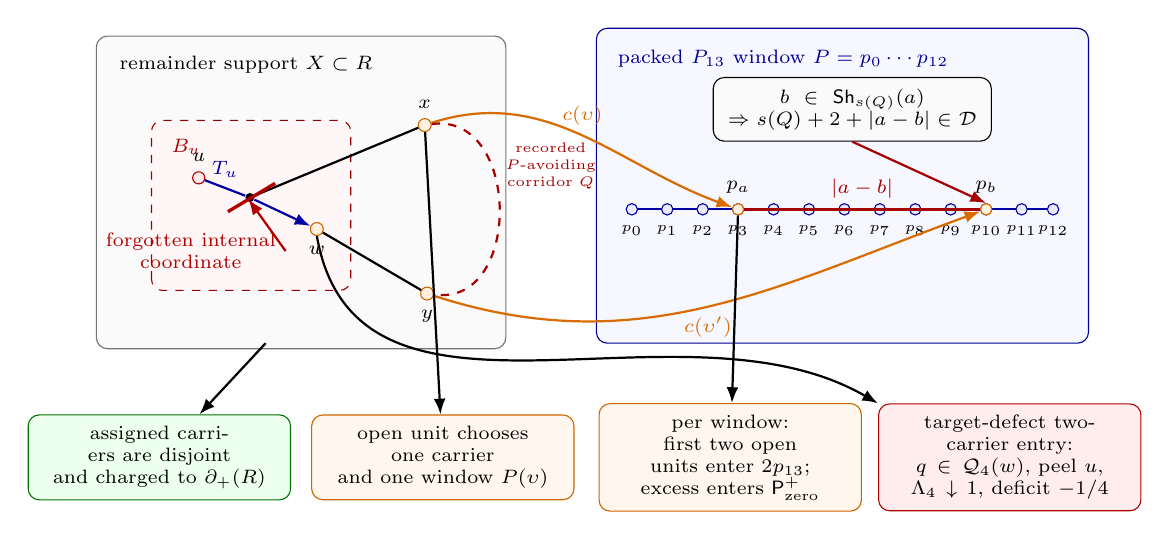
\begin{tikzpicture}[
vtx/.style={circle,fill=black,inner sep=1.15pt},
bd/.style={circle,draw=orange!80!black,fill=orange!12,inner sep=1.65pt},
winv/.style={circle,draw=blue!65!black,fill=blue!8,inner sep=1.45pt},
load/.style={circle,draw=red!70!black,fill=red!8,inner sep=1.55pt},
box/.style={rectangle,rounded corners,draw,fill=black!2,align=center,inner sep=4pt,text width=3.00cm},
good/.style={rectangle,rounded corners,draw=green!45!black,fill=green!7,align=center,inner sep=4pt,text width=3.05cm},
warn/.style={rectangle,rounded corners,draw=orange!80!black,fill=orange!7,align=center,inner sep=4pt,text width=3.05cm},
bad/.style={rectangle,rounded corners,draw=red!70!black,fill=red!7,align=center,inner sep=4pt,text width=3.05cm},
arr/.style={-{Latex[length=2mm]},thick},
car/.style={-{Latex[length=2mm]},thick,orange!85!black},
trace/.style={-{Latex[length=2mm]},thick,blue!65!black},
every node/.style={font=\scriptsize}
]
\draw[rounded corners,fill=black!2,draw=black!55] (-6.35,-1.62) rectangle (-1.15,2.35);
\node[anchor=north west] at (-6.18,2.22) {remainder support \(X\subset R\)};
\draw[rounded corners,fill=red!3,draw=red!60!black,dashed] (-5.65,-0.88) rectangle (-3.12,1.28);
\node[anchor=north west,red!65!black] at (-5.52,1.17) {\(B_u\)};

\node[load,label=above:\(u\)] (u) at (-5.05,0.55) {};
\node[vtx] (a) at (-4.40,0.30) {};
\node[bd,label=below:\(w\)] (w) at (-3.55,-0.10) {};
\node[bd,label=above:\(x\)] (x) at (-2.18,1.22) {};
\node[bd,label=below:\(y\)] (y) at (-2.15,-0.92) {};
\draw[trace] (u)--node[above] {\(T_u\)} (a)--(w);
\draw[thick] (a)--(x);
\draw[thick] (w)--(y);
\draw[red!70!black,very thick] (-4.68,0.12)--(-4.08,0.48);
\node[red!70!black,align=center] (forgot) at (-5.15,-0.38) {forgotten internal\\coordinate};
\draw[arr,red!70!black] (forgot.east) -- (-4.42,0.28);

\draw[rounded corners,fill=blue!3,draw=blue!60!black] (0.00,-1.55) rectangle (6.25,2.45);
\node[anchor=north west,blue!60!black] at (0.15,2.30) {packed \(P_{13}\) window \(P=p_0\cdots p_{12}\)};
\draw[thick,blue!65!black] (0.45,0.15)--(5.80,0.15);
\foreach \i/\xpos in {0/0.45,1/0.90,2/1.35,3/1.80,4/2.25,5/2.70,6/3.15,7/3.60,8/4.05,9/4.50,10/4.95,11/5.40,12/5.80}
  \node[winv,label=below:{\(\scriptscriptstyle p_{\i}\)}] (p\i) at (\xpos,0.15) {};
\node[winv,draw=orange!85!black,fill=orange!12,label=above:\(p_a\)] (pa) at (1.80,0.15) {};
\node[winv,draw=orange!85!black,fill=orange!12,label=above:\(p_b\)] (pb) at (4.95,0.15) {};

\draw[car] (x) to[out=18,in=160] node[above] {\(c(\upsilon)\)} (pa);
\draw[car] (y) to[out=-18,in=-160] node[below] {\(c(\upsilon')\)} (pb);
\draw[dashed,thick,red!65!black] (x) to[out=8,in=-8,looseness=1.35] (y);
\node[red!65!black,align=center,text width=1.45cm,font=\tiny] at (-0.58,0.70)
{recorded\\\(P\)-avoiding\\corridor \(Q\)};
\draw[very thick,red!65!black] (pa)--node[above,sloped] {\(|a-b|\)} (pb);
\node[box,text width=3.25cm] (shadow) at (3.25,1.42)
{\(b\in\Sh_{s(Q)}(a)\)\\\(\Rightarrow s(Q)+2+|a-b|\in\Pow\)};
\draw[arr,red!65!black] (shadow.south)--(pb.north);

\node[good] (defp) at (-5.55,-3.00)
{assigned carriers are disjoint\\and charged to \(\defp(R)\)};
\node[warn] (blocker) at (-1.95,-3.00)
{open unit chooses one carrier\\and one window \(P(\upsilon)\)};
\node[warn] (window) at (1.70,-3.00)
{per window:\\first two open units enter \(2p_{13}\);\\excess enters \(\mathsf P_{\rm zero}^{+}\)};
\node[bad] (peel) at (5.25,-3.00)
{target-defect two-carrier entry:\\\(q\in\mathcal Q_4(w)\), peel \(u\),\\\(\Lambda_4\downarrow1\), deficit \(-1/4\)};
\draw[arr] (-4.20,-1.55)--(defp);
\draw[arr] (x)--(blocker);
\draw[arr] (pa)--(window);
\draw[arr] (w.south) to[out=-80,in=150] (peel.north west);
\end{tikzpicture}%
}
\caption[Exit-(4) attachment to a packed \(P_{13}\) window]{Exit-\textup{(4)}
attachment to a packed \(P_{13}\) window and the associated accounting.  A
target-defect pressure token for the entry \(\xi=(X,w,u,B_u)\) forgets a
declared \(u\)-supported coordinate using an internal edge of \(B_u\).  The
witnessing event must also use the exterior of \(X\), so cut parity gives at
least two boundary carriers.  Carriers assigned by the \(2/3\)-pressure ledger
are pairwise disjoint and are counted once in \(\defp(R)\).  An unabsorbed
pressure unit chooses the lexicographically first carrier \(c(\upsilon)\);
because \(X\) is a component of the \(P_{13}\)-free remainder, the other
endpoint lies in the packed-window set, and the disjointness of the packing
gives a unique window \(P(\upsilon)\).  Thus
\(\mathsf P_{\rm open}=\sum_P B_{\rm open}(P)\).  On each window, the first two
open units form the base term \(2p_{13}\); any third open unit forms an
overload triple.  Routed triples leave through the direct dyadic certificate,
an unused boundary absorber, a proper-compression or delocalization absorber,
or the Type B fan-window handoff.  If two open units have a recorded
\(P\)-avoiding corridor \(Q\) with \(b\in\Sh_{s(Q)}(a)\), the displayed cycle
has length \(s(Q)+2+|a-b|\in\Pow\), so the triple is routed.  The only
surviving excess is the zero-shadow term in
\(\mathsf P_{\rm open}\le2p_{13}+\mathsf P_{\rm zero}^{+}\).  Independently of
that auxiliary window audit, every surviving target-defect two-carrier entry is
a canonical \textup{(Q3)} exit-\textup{(4)} quotient, so
\cref{lem:typeA-pressure-is-exit4-peel,lem:typeA-exit4-finite-descent} peel
the routed load \(u\), decrease the remaining deficit by exactly \(1/4\), and
strictly decrease \(\Lambda_4\).}
\label{fig:exit4-p13-attachment-accounting}
\end{figure}

\begin{definition}[Same-window overload triples]%
\label[definition]{def:typeA-same-window-overload-triple}
For a packed window \(P\in\mathcal P\), put
\[
\mathcal U(P)=
\{\upsilon\in\mathcal U_{\rm press}\setminus\mathcal U_{\rm abs}:
P(\upsilon)=P\}.
\]
A \emph{same-window overload triple at \(P\)} is a three-element subset
\(\mathcal T\subseteq\mathcal U(P)\).  If
\(\upsilon\in\mathcal T\), write
\[
c(\upsilon)=(x_\upsilon,x_\upsilon p_{a(\upsilon)}),
\qquad
P=p_0p_1\cdots p_{12},
\]
for its canonical window carrier and its window index.

The triple \(\mathcal T\) is \emph{routed} if at least one of the following
certificates is present.
\begin{enumerate}[label=(O\arabic*), leftmargin=2.2em]
\item \emph{Direct dyadic window certificate.}  The pressure records of one or
two units in \(\mathcal T\), or an explicitly recorded \(P\)-avoiding corridor
between their canonical window carriers, together with one or two subpaths of
\(P\), contain a simple cycle of length in \(\Pow\).  This includes the direct
same-window and two-window cycle configurations covered by
\cref{lem:typeB-direct-fan-window-cycles,lem:typeB-two-window-cycles}.
\item \emph{Unused boundary-incidence certificate.}  Some
\(\upsilon=(\xi,j)\in\mathcal T\), with \(\xi=(X,w,u,B_u)\), has an oriented
boundary incidence \(c\in\partial_E X\) which is not used by any set
\(A(\xi')\) in the \(2/3\)-pressure ledger and is not assigned to any absorbed
pressure unit.
\item \emph{Profile-dependence certificate.}  A subfamily of profile
coordinates belonging to units of \(\mathcal T\) is rank-reducing under a
functional admissible quotient, and the routing supplied by
\cref{lem:typeA-profile-pressure-dependence-routing} is a proper-support
compression or one of the delocalization alternatives already removed by the
branch split.
\item \emph{Type B fan-window certificate.}  Two units of \(\mathcal T\)
determine fan-closed ports or cubic-closed fan neighbours in an assigned
Type B fan-window profile, with the window incidences and non-window incidences
required by
\cref{lem:compatible-pair-fan-closure,def:typeB-bridge-statements}.  Thus the
local B1 entry is available, and any failure of cross-center disjointness is a
B2 overlap obstruction in the sense of
\cref{lem:typeB-bridge-to-overlap}.
\end{enumerate}
A same-window overload triple is \emph{primitive} if it is not routed.
\end{definition}

\begin{lemma}[Routed overload triples do not remain open]%
\label[lemma]{lem:typeA-routed-overload-not-open}
Work on a branch where the direct dyadic cycle alternatives, the type
\textup{(A1)} boundary absorbers, the type \textup{(A2)}
proper-compression or delocalization absorbers, and the Type B fan-window handoff
have all been applied.  Then every surviving same-window overload triple is
primitive.
\end{lemma}

\begin{proof}
Let \(\mathcal T\) be a same-window overload triple.  If (O1) holds, the
displayed certificate is a power-of-two cycle in \(G\), contradicting the
standing counterexample hypothesis.  If (O2) holds, the indicated boundary
incidence is an admissible absorber of type \textup{(A1)} in
\cref{def:typeA-pressure-absorbers}.  Since the absorber assignment is maximal,
the corresponding pressure unit cannot still be open.  If (O3) holds,
\cref{lem:typeA-profile-pressure-dependence-routing} supplies an absorber of
type \textup{(A2)} whose conclusion is proper compression or delocalization;
on the stated branch such a unit has routed away from the open pressure
ledger.  If (O4) holds, the data are exactly Type B fan-window data.  The local
B1 entry is supplied by \cref{def:typeB-bridge-statements}; if disjointness
fails, \cref{lem:typeB-bridge-to-overlap} records the B2 residual.  In either
case the triple is no longer an open Type A pressure overload.  Therefore a
surviving same-window overload triple has none of (O1)--(O4), and is primitive
by definition.
\end{proof}

\begin{definition}[Primitive same-window overload excess]%
\label[definition]{def:typeA-primitive-window-overload-excess}
Assume the branch of \cref{lem:typeA-routed-overload-not-open}.  A packed
window \(P\) is \emph{primitive-overloaded} if
\[
B_{\rm open}(P)=|\mathcal U(P)|\ge3
\]
and the lexicographically first three-element subset of \(\mathcal U(P)\) is a
primitive same-window overload triple.  The \emph{primitive overload excess} is
\[
\mathsf P_{\rm prim}^{+}
=
\sum_{\substack{P\in\mathcal P\\ P\text{ primitive-overloaded}}}
\bigl(B_{\rm open}(P)-2\bigr).
\]
\end{definition}

\begin{definition}[Window attachment shadows]\label[definition]{def:typeA-window-attachment-shadow}
Let \(P=p_0p_1\cdots p_{12}\) be a packed window.  For an integer
\(s\ge0\), define the forbidden distance set
\[
D_s=\{d\in\{0,\ldots,12\}:s+2+d\in\Pow\}.
\]
For an attachment index \(a\in\{0,\ldots,12\}\), define its
\emph{\(s\)-shadow} on \(P\) by
\[
\Sh_s(a)
=
\{b\in\{0,\ldots,12\}: |a-b|\in D_s\}.
\]
Equivalently,
\[
b\in\Sh_s(a)
\quad\Longleftrightarrow\quad
C_s(\{a\},\{b\})=0
\]
for the \(P_{13}\)-label relation \(C_s\) of the main window algebra.
\end{definition}

\begin{lemma}[Exact singleton-shadow table]\label[lemma]{lem:typeA-singleton-shadow-table}
For every \(s\ge0\),
\[
D_s=\{2^q-s-2:q\ge2,\ 0\le2^q-s-2\le12\}.
\]
In particular,
\[
\begin{array}{c|l}
s & D_s\\
\hline
0&\{2,6\}\\
1&\{1,5\}\\
2&\{0,4,12\}\\
3&\{3,11\}\\
4&\{2,10\}\\
5&\{1,9\}\\
6&\{0,8\}\\
7&\{7\}\\
8&\{6\}\\
9&\{5\}\\
10&\{4\}\\
11&\{3\}\\
12&\{2\}\\
13&\{1\}\\
14&\{0\}\\
15,16,17&\varnothing\\
18&\{12\}\\
19&\{11\}\\
20&\{10\}\\
21&\{9\}\\
22&\{8\}\\
23&\{7\}\\
24&\{6\}\\
25&\{5\}\\
26&\{4\}\\
27&\{3\}\\
28&\{2\}\\
29&\{1\}\\
30&\{0\}.
\end{array}
\]
For \(s\ge18\), the set \(D_s\) has at most one element.
\end{lemma}

\begin{proof}
By \cref{def:typeA-window-attachment-shadow}, \(d\in D_s\) exactly when
\(s+2+d=2^q\) for some \(q\ge2\).  This is equivalent to
\[
d=2^q-s-2
\]
with \(0\le d\le12\), giving the displayed formula.  The table is obtained by
substituting \(s=0,\ldots,30\) into this formula.  If \(s\ge18\), then
\([s+2,s+14]\subseteq[20,\infty)\).  Consecutive powers of two in
\([16,\infty)\) differ by at least \(16>12\), so the interval
\([s+2,s+14]\) contains at most one power of two.  Hence \(D_s\) has at most
one element.
\end{proof}

\begin{definition}[Recorded window-shadow hit]\label[definition]{def:typeA-recorded-window-shadow-hit}
Let \(\upsilon,\upsilon'\in\mathcal U(P)\) be distinct open pressure units on
the same packed window \(P=p_0\cdots p_{12}\), with canonical carriers
\[
c(\upsilon)=(x,xp_a),
\qquad
c(\upsilon')=(y,yp_b).
\]
A \emph{recorded \(P\)-avoiding corridor} from \(\upsilon\) to \(\upsilon'\)
is a simple \(x\)-\(y\) path \(Q\) in \(G-V(P)\), recorded in the actual
pressure data of one or both units or in the Type B fan-window handoff data,
whose internal vertices avoid \(P\) and whose first and last edges are not
the canonical carrier edges \(xp_a,yp_b\).  Its length is denoted
\(s(Q)=|E(Q)|\).

The ordered pair \((\upsilon,\upsilon')\) has a \emph{recorded window-shadow
hit} if the two canonical carrier edges \(xp_a\) and \(yp_b\) are distinct,
such a corridor \(Q\) exists, and
\[
b\in\Sh_{s(Q)}(a).
\]
When \(x=y\), the corridor \(Q\) may be the trivial length-zero path; the
distinct-carrier condition then says \(a\ne b\).
\end{definition}

\begin{lemma}[Window-shadow hits are direct dyadic certificates]%
\label[lemma]{lem:typeA-window-shadow-hit-routes}
If two open pressure units on the same packed window have a recorded
window-shadow hit, then every same-window overload triple containing them is
routed by certificate \textup{(O1)} of
\cref{def:typeA-same-window-overload-triple}.
\end{lemma}

\begin{proof}
Use the notation of \cref{def:typeA-recorded-window-shadow-hit}.  Since
\(b\in\Sh_{s(Q)}(a)\), the definition of the shadow gives
\[
s(Q)+2+|a-b|\in\Pow.
\]
The path
\[
x\,Q\,y\,p_b\,P\,p_a\,x
\]
is a simple cycle.  Indeed, \(Q\) lies in \(G-V(P)\), the segment \(p_bPp_a\)
lies in the induced path \(P\), and the only edges between the two pieces used
in the display are the two distinct canonical carrier edges \(yp_b\) and
\(xp_a\).  If \(x=y\), then \(Q\) is the trivial path and distinctness of the
carrier edges gives \(a\ne b\), so the displayed cycle is
\(x p_b P p_a x\).  In all cases the length is exactly
\(s(Q)+2+|a-b|\), hence is a power of two.  This is a direct dyadic window
certificate, which is certificate \textup{(O1)}.
\end{proof}

\begin{definition}[Zero-shadow primitive excess]%
\label[definition]{def:typeA-zero-shadow-primitive-excess}
Assume the branch of \cref{lem:typeA-routed-overload-not-open}.  A
primitive-overloaded packed window \(P\) is \emph{zero-shadow} if the
set \(\mathcal U(P)\) has no pair of distinct open units with a recorded
window-shadow hit.  The \emph{zero-shadow primitive excess} is
\[
\mathsf P_{\rm zero}^{+}
=
\sum_{\substack{P\in\mathcal P\\ P\text{ zero-shadow}}}
\bigl(B_{\rm open}(P)-2\bigr).
\]
\end{definition}

\begin{lemma}[Primitive excess equals zero-shadow excess after window-shadow routing]%
\label[lemma]{lem:typeA-primitive-excess-zero-shadow}
Work on a branch where the routed overload triples of
\cref{def:typeA-same-window-overload-triple} have been removed.  Then
\[
\mathsf P_{\rm prim}^{+}=\mathsf P_{\rm zero}^{+}.
\]
\end{lemma}

\begin{proof}
Let \(P\) be primitive-overloaded.  Its lexicographically first three open
units form a surviving same-window overload triple.  If some pair in that
triple had a recorded window-shadow hit, then
\cref{lem:typeA-window-shadow-hit-routes} would route the triple by
certificate \textup{(O1)}, contrary to the branch hypothesis.  More generally,
if any distinct pair \(\upsilon,\upsilon'\in\mathcal U(P)\) had a recorded
window-shadow hit, then, since \(B_{\rm open}(P)\ge3\), choosing any third
unit of \(\mathcal U(P)\) would give a same-window overload triple routed by
\textup{(O1)}.  Hence no pair in \(\mathcal U(P)\) has a recorded
window-shadow hit, so \(P\) is zero-shadow.  Therefore every summand counted by
\(\mathsf P_{\rm prim}^{+}\) is counted by \(\mathsf P_{\rm zero}^{+}\).
Conversely, a zero-shadow window is primitive-overloaded by definition, so
every summand counted by \(\mathsf P_{\rm zero}^{+}\) is counted by
\(\mathsf P_{\rm prim}^{+}\).
\end{proof}

\begin{lemma}[Open pressure after routed overloads]%
\label[lemma]{lem:typeA-open-pressure-zero-shadow-excess}
On a branch where the routed overload triples of
\cref{def:typeA-same-window-overload-triple} have been removed,
\[
\mathsf P_{\rm open}\le 2p_{13}+\mathsf P_{\rm zero}^{+}.
\]
\end{lemma}

\begin{proof}
By \cref{lem:typeA-open-window-blocker-count},
\[
\mathsf P_{\rm open}=\sum_{P\in\mathcal P}B_{\rm open}(P).
\]
If \(B_{\rm open}(P)\le2\), then its contribution is at most \(2\).  If
\(B_{\rm open}(P)\ge3\), then the lexicographically first three-element subset
of \(\mathcal U(P)\) is a surviving same-window overload triple.  By
\cref{lem:typeA-routed-overload-not-open}, it is primitive, so \(P\) is
primitive-overloaded.  If its first triple had a recorded window-shadow hit,
\cref{lem:typeA-window-shadow-hit-routes} would route it by certificate
\textup{(O1)}, contrary to the branch hypothesis.  If any other pair in
\(\mathcal U(P)\) had a recorded window-shadow hit, that pair together with
any third open unit would give a routed same-window overload triple, again
contrary to the branch hypothesis.  Hence \(P\) is zero-shadow, and its excess
\(B_{\rm open}(P)-2\) is one summand of
\(\mathsf P_{\rm zero}^{+}\).  Therefore, for every packed window \(P\),
\[
B_{\rm open}(P)\le 2+
\mathbf 1_{\{P\text{ zero-shadow}\}}\bigl(B_{\rm open}(P)-2\bigr)
\]
with no overlap between windows.  Summing this pointwise inequality over
\(P\in\mathcal P\) gives the result.
\end{proof}

\begin{lemma}[Window-blocker accounting audit]%
\label[lemma]{lem:typeA-window-blocker-accounting-audit}
On a branch where the routed overload triples of
\cref{def:typeA-same-window-overload-triple} have been removed, every open
pressure unit is counted in exactly one of the following two places:
\begin{enumerate}[label=(\alph*), leftmargin=2.2em]
\item among the first two open units assigned to its packed window, contributing
to the base term \(2p_{13}\);
\item among the excess units of a zero-shadow primitive-overloaded packed
window, contributing to \(\mathsf P_{\rm zero}^{+}\).
\end{enumerate}
No open unit is counted for two packed windows, and every same-window overload
not counted in \(\mathsf P_{\rm zero}^{+}\) has routed through one of
\textup{(O1)}--\textup{(O4)}.
\end{lemma}

\begin{proof}
\Cref{lem:typeA-open-window-blocker-count} partitions the open pressure units
by the unique packed window \(P(\upsilon)\).  Inside a fixed packed window,
choose the first two units in the global lexicographic order as the base units;
if fewer than two units are present, all units are base units.  Any remaining
unit exists only when \(B_{\rm open}(P)\ge3\).  On the stated branch, the first
three units then form a surviving same-window overload triple.  If that triple
were routed by one of \textup{(O1)}--\textup{(O4)}, the branch would have
removed that overload before \(\mathsf P_{\rm open}\) is counted.  Hence, for
an open residual unit, the triple is not routed.
\Cref{lem:typeA-routed-overload-not-open} makes it primitive, and
\cref{lem:typeA-window-shadow-hit-routes} removes every same-window overload
triple containing a pair with a recorded window-shadow hit.  Since
\(B_{\rm open}(P)\ge3\), any recorded-hit pair in \(\mathcal U(P)\) would lie
in such a triple.  Thus the window is zero-shadow, and all units beyond the
first two are counted in the summand \(B_{\rm open}(P)-2\) of
\(\mathsf P_{\rm zero}^{+}\).  The packed windows are vertex-disjoint and the
assignment \(P(\upsilon)\) is single-valued, so no open unit can appear in two
window classes.  These two alternatives exhaust the open units because they are
applied after the exact partition of
\cref{lem:typeA-open-window-blocker-count}.
\end{proof}

\begin{lemma}[Exhaustion of the final open-pressure charge]%
\label[lemma]{lem:typeA-final-open-pressure-exhaustion}
Assume the type \textup{(A2)} absorbers of
\cref{def:typeA-pressure-absorbers} have routed to their
proper-compression or delocalization alternatives, and assume the routed
overload triples of \cref{def:typeA-same-window-overload-triple} have been
removed.  Then the surviving open pressure admits a disjoint partition
\[
\mathcal U_{\rm press}\setminus\mathcal U_{\rm abs}
=
\mathcal U_{\rm base}\sqcup\mathcal U_{\rm zero}
\]
such that
\[
|\mathcal U_{\rm base}|\le2p_{13},
\qquad
|\mathcal U_{\rm zero}|=\mathsf P_{\rm zero}^{+},
\]
and hence
\[
3\tilde N-\mathsf P_{\rm open}\le\defp(R),
\qquad
\mathsf P_{\rm open}\le2p_{13}+\mathsf P_{\rm zero}^{+}.
\]
\end{lemma}

\begin{proof}
The boundary-incidence inequality
\[
3\tilde N-\mathsf P_{\rm open}\le\defp(R)
\]
is \cref{lem:typeA-pressure-absorber-no-overcount} after the type
\textup{(A2)} alternatives have routed away.

It remains to identify the open units.  By
\cref{lem:typeA-open-window-blocker-count}, every open pressure unit has a
unique packed window \(P(\upsilon)\).  For a fixed window \(P\), order
\(\mathcal U(P)\) by the global lexicographic order.  Put the first two units,
if present, in \(\mathcal U_{\rm base}\).  Since there are \(p_{13}\) packed
windows, this gives \(|\mathcal U_{\rm base}|\le2p_{13}\).

Let \(\upsilon\) be any remaining open unit on \(P\).  Then
\(B_{\rm open}(P)\ge3\).  The first three units of \(\mathcal U(P)\) form a
same-window overload triple.  If that triple were routed by one of
\textup{(O1)}--\textup{(O4)}, it would have been removed before the present
open-pressure ledger was formed.  Hence the triple is primitive and \(P\) is
primitive-overloaded.  If any pair in \(\mathcal U(P)\) had a recorded
window-shadow hit, that pair and any third open unit of \(\mathcal U(P)\) would
form a same-window overload triple routed by \textup{(O1)} via
\cref{lem:typeA-window-shadow-hit-routes}; this is again excluded on the
present branch.  Therefore \(P\) is zero-shadow.  Put every unit of
\(\mathcal U(P)\) after the first two in \(\mathcal U_{\rm zero}\).

The preceding paragraph applies to every open unit not in
\(\mathcal U_{\rm base}\), and the construction is window-by-window, so the two
sets are disjoint and cover
\(\mathcal U_{\rm press}\setminus\mathcal U_{\rm abs}\).  For a zero-shadow
window \(P\), exactly \(B_{\rm open}(P)-2\) units are placed in
\(\mathcal U_{\rm zero}\), and no non-zero-shadow window contributes to
\(\mathcal U_{\rm zero}\).  Summing over \(P\) gives
\[
|\mathcal U_{\rm zero}|
=
\sum_{\substack{P\in\mathcal P\\ P\text{ zero-shadow}}}
\bigl(B_{\rm open}(P)-2\bigr)
=
\mathsf P_{\rm zero}^{+}.
\]
The last displayed inequality follows from
\[
\mathsf P_{\rm open}
=|\mathcal U_{\rm press}\setminus\mathcal U_{\rm abs}|
=|\mathcal U_{\rm base}|+|\mathcal U_{\rm zero}|.
\]
\end{proof}

\begin{proposition}[Exit-(4) closure from zero-shadow slack]%
\label[proposition]{prop:typeA-exit4-closure-from-zero-shadow}
Assume \cref{def:near-cubic-spine}.  Work on a branch where the type
\textup{(A2)} absorbers of \cref{def:typeA-pressure-absorbers} have routed to
their proper-compression or delocalization alternatives, and where the routed
overload triples of \cref{def:typeA-same-window-overload-triple} have been
removed.  If
\[
\limsup_{|R|\to\infty}
\frac{\mathsf P_{\rm zero}^{+}}{|R|}
<
\varepsilon_{\rm prim},
\]
where
\[
\varepsilon_{\rm press}
=
12\left(\frac14-\tau_{\rm win}\right)-\tau_{\rm win},
\qquad
\varepsilon_{\rm prim}
=
\varepsilon_{\rm press}
-
\frac{2\theta_{\rm win}}{1-13\theta_{\rm win}}
=0.00330339423\ldots .
\]
then the target-defect exit-\textup{(4)} residual is impossible.
\end{proposition}

\begin{proof}
By \cref{lem:typeA-final-open-pressure-exhaustion},
\[
\mathsf P_{\rm open}\le 2p_{13}+\mathsf P_{\rm zero}^{+}.
\]
The near-cubic \(P_{13}\)-density bound gives
\[
p_{13}\le\theta_{\rm win}n+o(n).
\]
Writing \(\theta=p_{13}/n\), the remainder size is
\[
|R|=(1-13\theta)n+o(n),
\]
and \(2\theta/(1-13\theta)\) is increasing for
\(0\le\theta<1/13\).  Therefore
\[
\limsup_{|R|\to\infty}\frac{2p_{13}}{|R|}
\le
\frac{2\theta_{\rm win}}{1-13\theta_{\rm win}}.
\]
Hence the displayed hypothesis implies
\[
\limsup_{|R|\to\infty}\frac{\mathsf P_{\rm open}}{|R|}
<
\frac{2\theta_{\rm win}}{1-13\theta_{\rm win}}
+
\varepsilon_{\rm prim}
=
\varepsilon_{\rm press}.
\]
\Cref{prop:typeA-exit4-closure-from-open-pressure} now closes the
target-defect exit-\textup{(4)} residual.
\end{proof}

\begin{remark}[Numerical size of the final shadow residual]%
\label[remark]{rem:typeA-zero-shadow-numerics}
Since
\[
\frac{p_{13}}{|R|}
\le
\frac{\theta_{\rm win}}{1-13\theta_{\rm win}}+o(1)
=0.01521165789\ldots+o(1),
\]
the available slack
\[
\varepsilon_{\rm prim}=0.00330339423\ldots
\]
is exactly
\[
\frac{\varepsilon_{\rm prim}}
{\theta_{\rm win}/(1-13\theta_{\rm win})}
=0.2171620118\ldots
\]
zero-shadow excess units per packed window on average.  Thus the
zero-shadow criterion alone leaves only residuals satisfying
\[
\mathsf P_{\rm zero}^{+}
\ge
0.2171620118\ldots\,p_{13}-o(|R|).
\]
Every packed window contributing to this sum carries at least a third open
blocker, no pair of open blockers on that window has a recorded
\(C_s\)-shadow hit, and the corresponding open units have no unused boundary
absorber, no proper-compression or delocalization absorber, and no Type B
fan-window handoff.
\end{remark}

\begin{definition}[Same-window open-blocker cap]%
\label[definition]{def:typeA-same-window-open-blocker-cap}
The open-pressure ledger satisfies the \emph{same-window two-blocker cap} if
there is an exceptional set
\[
\mathcal E_{\rm win}\subseteq
\mathcal U_{\rm press}\setminus\mathcal U_{\rm abs}
\]
with \(|\mathcal E_{\rm win}|=o(|R|)\) such that, after deleting
\(\mathcal E_{\rm win}\), every packed window \(P\in\mathcal P\) receives at
most two canonical open blockers:
\[
|\{\upsilon\in
(\mathcal U_{\rm press}\setminus\mathcal U_{\rm abs})\setminus
\mathcal E_{\rm win}:P(\upsilon)=P\}|
\le2 .
\]
\end{definition}

\begin{lemma}[The two-blocker cap has sublinear overload excess]%
\label[lemma]{lem:typeA-same-window-cap-overload-excess}
If the same-window two-blocker cap of
\cref{def:typeA-same-window-open-blocker-cap} holds, then
\[
\mathsf P_{\rm prim}^{+}=o(|R|)
\qquad\text{and}\qquad
\mathsf P_{\rm zero}^{+}=o(|R|).
\]
\end{lemma}

\begin{proof}
Let \(\mathcal E_{\rm win}\) be the exceptional set in
\cref{def:typeA-same-window-open-blocker-cap}.  For a fixed packed window
\(P\), write \(e(P)=|\mathcal E_{\rm win}\cap\mathcal U(P)|\).  After deleting
\(\mathcal E_{\rm win}\), at most two units remain on \(P\), so
\[
\max\{0,B_{\rm open}(P)-2\}\le e(P).
\]
The primitive overload excess is bounded by the total overload excess:
\[
\mathsf P_{\rm prim}^{+}
\le
\sum_{P\in\mathcal P}\max\{0,B_{\rm open}(P)-2\}
\le
\sum_{P\in\mathcal P}e(P)
=|\mathcal E_{\rm win}|
=o(|R|).
\]
The same displayed total overload excess also bounds
\(\mathsf P_{\rm zero}^{+}\), since zero-shadow windows are a subfamily of the
packed windows.
\end{proof}

\begin{lemma}[Numerical window-blocker squeeze]%
\label[lemma]{lem:typeA-window-blocker-numerics}
Assume \cref{def:near-cubic-spine}.  If the same-window two-blocker cap of
\cref{def:typeA-same-window-open-blocker-cap} holds, then
\[
\limsup_{|R|\to\infty}\frac{\mathsf P_{\rm open}}{|R|}
\le
\frac{2\theta_{\rm win}}{1-13\theta_{\rm win}}
=0.03042331579\ldots
<
0.03372671002\ldots
=\varepsilon_{\rm press}.
\]
\end{lemma}

\begin{proof}
By \cref{lem:typeA-open-window-blocker-count} and the same-window cap,
\[
\mathsf P_{\rm open}\le 2p_{13}+o(|R|).
\]
The near-cubic \(P_{13}\)-density bound gives
\[
p_{13}\le\theta_{\rm win}n+o(n).
\]
Writing \(\theta=p_{13}/n\), the remainder size is
\[
|R|=(1-13\theta)n+o(n),
\]
and the function \(2\theta/(1-13\theta)\) is increasing on the relevant
interval \(0\le\theta<1/13\).  Therefore
\[
\limsup_{|R|\to\infty}\frac{\mathsf P_{\rm open}}{|R|}
\le
\frac{2\theta_{\rm win}}{1-13\theta_{\rm win}}.
\]
Substituting \(\theta_{\rm win}=0.01270017798\ldots\) gives
\[
\frac{2\theta_{\rm win}}{1-13\theta_{\rm win}}
=0.03042331579\ldots .
\]
The open-pressure threshold from
\cref{prop:typeA-exit4-closure-from-open-pressure} is
\[
\varepsilon_{\rm press}
=12\left(\frac14-\tau_{\rm win}\right)-\tau_{\rm win}
=0.03372671002\ldots ,
\]
so the displayed bound lies strictly below the threshold.
\end{proof}

\begin{proposition}[Exit-(4) closure from the same-window cap]%
\label[proposition]{prop:typeA-exit4-closure-from-window-blockers}
Assume \cref{def:near-cubic-spine}.  On a branch where all dependence
absorbers of type \textup{(A2)} have routed to their proper-compression or
delocalization alternatives, the target-defect exit-(4) residual is impossible
whenever the same-window two-blocker cap of
\cref{def:typeA-same-window-open-blocker-cap} holds.
\end{proposition}

\begin{proof}
By \cref{lem:typeA-window-blocker-numerics}, the same-window cap gives
\[
\limsup_{|R|\to\infty}\frac{\mathsf P_{\rm open}}{|R|}
<
\varepsilon_{\rm press}.
\]
The conclusion is exactly
\cref{prop:typeA-exit4-closure-from-open-pressure}.
\end{proof}

\begin{figure}[t]
\centering
\resizebox{0.78\textwidth}{!}{%
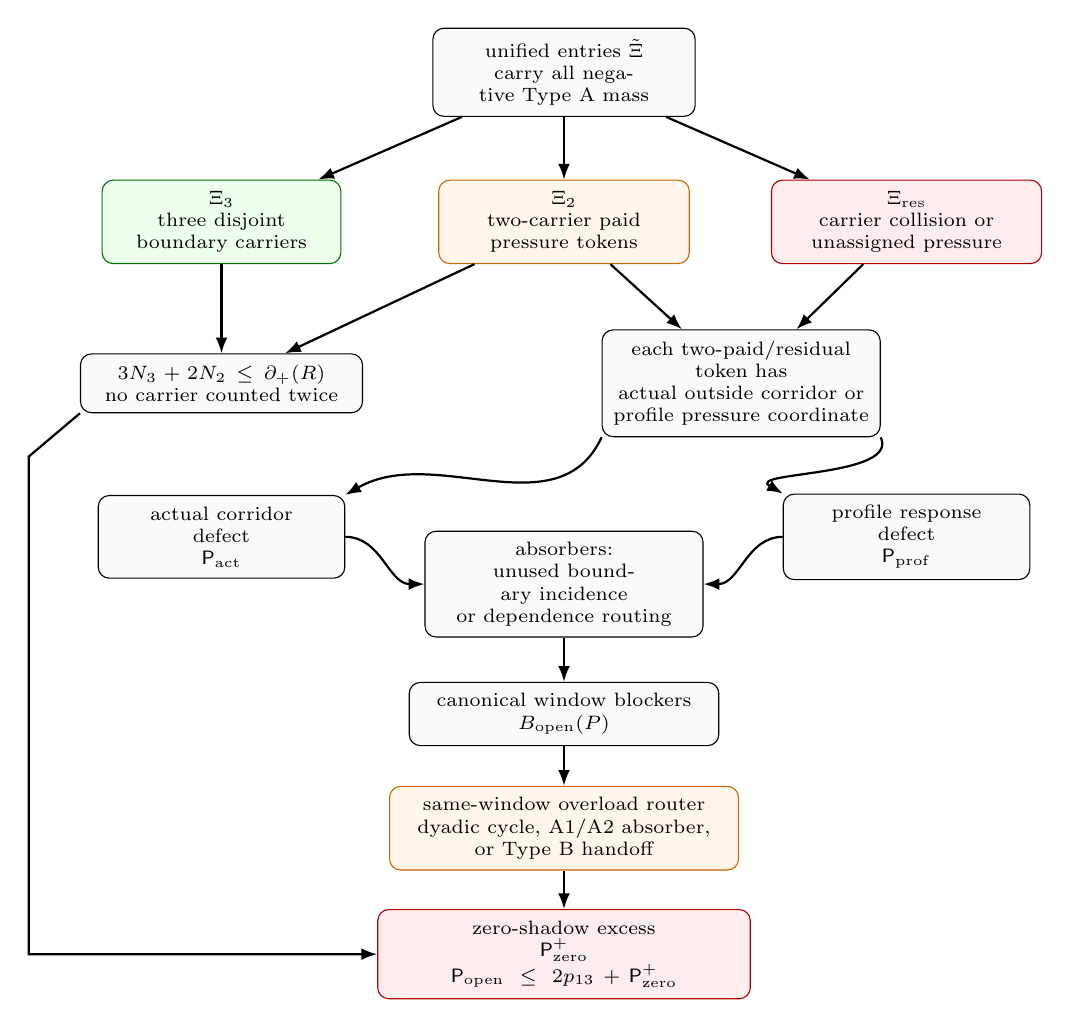
\begin{tikzpicture}[
box/.style={rectangle,rounded corners,draw,fill=black!2,align=center,inner sep=4pt,text width=2.55cm},
wide/.style={rectangle,rounded corners,draw,fill=black!2,align=center,inner sep=4pt,text width=3.05cm},
good/.style={rectangle,rounded corners,draw=green!45!black,fill=green!7,align=center,inner sep=4pt,text width=2.75cm},
warn/.style={rectangle,rounded corners,draw=orange!80!black,fill=orange!8,align=center,inner sep=4pt,text width=2.90cm},
bad/.style={rectangle,rounded corners,draw=red!70!black,fill=red!7,align=center,inner sep=4pt,text width=3.15cm},
arr/.style={-{Latex[length=2mm]},thick},
every node/.style={font=\scriptsize}
]
\node[wide] (entries) at (0,2.15) {unified entries \(\tilde\Xi\)\\carry all negative Type A mass};
\node[good] (three) at (-4.35,0.25) {\(\Xi_3\)\\three disjoint\\boundary carriers};
\node[warn] (two) at (0,0.25) {\(\Xi_2\)\\two-carrier paid\\pressure tokens};
\node[bad] (res) at (4.35,0.25) {\(\Xi_{\rm res}\)\\carrier collision or\\unassigned pressure};
\draw[arr] (entries)--(three);
\draw[arr] (entries)--(two);
\draw[arr] (entries)--(res);
\node[box,text width=3.30cm] (ineq) at (-4.35,-1.80)
{\(3N_3+2N_2\le\defp(R)\)\\no carrier counted twice};
\node[box,text width=3.25cm] (record) at (2.25,-1.80)
{each two-paid/residual token has\\actual outside corridor or\\profile pressure coordinate};
\draw[arr] (three)--(ineq);
\draw[arr] (two)--(ineq);
\draw[arr] (two)--(record);
\draw[arr] (res)--(record);
\node[box,text width=2.85cm] (act) at (-4.35,-3.75)
{actual corridor\\defect\\\(\mathsf P_{\rm act}\)};
\node[box,text width=2.85cm] (prof) at (4.35,-3.75)
{profile response\\defect\\\(\mathsf P_{\rm prof}\)};
\draw[arr] (record.south west) to[out=-115,in=30] (act.north east);
\draw[arr] (record.south east) to[out=-65,in=150] (prof.north west);
\node[box,text width=3.25cm] (abs) at (0,-4.35)
{absorbers:\\unused boundary incidence\\or dependence routing};
\draw[arr] (act.east) to[out=0,in=180] (abs.west);
\draw[arr] (prof.west) to[out=180,in=0] (abs.east);
\node[box,text width=3.65cm] (win) at (0,-6.00)
{canonical window blockers\\\(B_{\rm open}(P)\)};
\node[warn,text width=4.15cm] (over) at (0,-7.45)
{same-window overload router\\dyadic cycle, A1/A2 absorber,\\or Type B handoff};
\node[bad,text width=4.45cm] (crit) at (0,-9.05)
{zero-shadow excess\\\(\mathsf P_{\rm zero}^{+}\)\\
\(\mathsf P_{\rm open}\le2p_{13}+\mathsf P_{\rm zero}^{+}\)};
\draw[arr] (ineq.south west) -- ++(-0.65,-0.55) |- (crit.west);
\draw[arr] (abs)--(win);
\draw[arr] (win)--(over);
\draw[arr] (over)--(crit);
\end{tikzpicture}%
}
\caption[External-pressure accounting for exit-(4) tokens]{External-pressure
accounting for exit-(4) target-defect tokens.  The three-carrier class is paid
directly by disjoint boundary incidences.  The two-carrier paid class receives
two disjoint boundary incidences and leaves one unit of pressure defect; this
class includes genuinely cheap two-carrier tokens and tokens whose additional
carriers collide with earlier ledger choices.  The unassigned class leaves
three units of pressure defect.  Each two-carrier paid or unassigned
target-defect token is represented by either an actual outside corridor in
\(G-X\) or by a profile-only exact response coordinate.  These give the exact
split
\(\mathsf P_{\rm ext}=\mathsf P_{\rm act}+\mathsf P_{\rm prof}\).  The
absorption ledger then assigns pressure units either to unused boundary
incidences, which improve the same \(\defp(R)\) count, or to profile-dependence
certificates, which route to proper-compression or delocalization alternatives.
Target-defective dependence outputs re-enter the pressure ledger instead of
being treated as absorbed.  The only pressure left in the surviving branch is
\(\mathsf P_{\rm open}\).  The window-blocker ledger assigns every open unit to
a unique packed \(P_{13}\)-window.  A same-window overload triple is routed
when it realizes a direct dyadic cycle, an unused boundary absorber, a
proper-compression or delocalization absorber, or a Type B fan-window handoff.
After these routed triples and their recorded window-shadow dyadic hits have
been removed, the only extra term beyond two blockers per window is the
zero-shadow primitive excess \(\mathsf P_{\rm zero}^{+}\), with
\(\mathsf P_{\rm open}\le2p_{13}+\mathsf P_{\rm zero}^{+}\).
Thus \cref{prop:typeA-exit4-closure-from-zero-shadow} closes the
branch whenever
\(\mathsf P_{\rm zero}^{+}<\varepsilon_{\rm prim}|R|-o(|R|)\).  The
same-window two-blocker cap is the special case
\(\mathsf P_{\rm zero}^{+}=o(|R|)\), where the strict numerical inequality is
\(2\theta_{\rm win}/(1-13\theta_{\rm win})
=0.03042331579\ldots<0.03372671002\ldots=\varepsilon_{\rm press}\).}
\label{fig:exit4-external-pressure-ledger}
\end{figure}

\begin{proposition}[Sharp external-pressure closure criterion]%
\label[proposition]{prop:typeA-external-pressure-criterion}
Assume \cref{def:near-cubic-spine}.  In the large-budget branch, suppose the
pressure ledger of \cref{def:typeA-pressure-ledger} satisfies
\[
\limsup_{|R|\to\infty}\frac{\mathsf P_{\rm ext}}{|R|}
<
\varepsilon_{\rm press},
\qquad
\varepsilon_{\rm press}
=
12\left(\frac14-\tau_{\rm win}\right)-\tau_{\rm win}.
\]
Then no minimal counterexample survives.  Numerically,
\[
\varepsilon_{\rm press}
=
12(0.02182513154\ldots)-0.22817486846\ldots
=0.03372671002\ldots .
\]
In particular, a sublinear external-pressure defect
\(\mathsf P_{\rm ext}=o(|R|)\) closes the branch.
\end{proposition}

\begin{proof}
By \cref{lem:typeA-unified-deficit,lem:typeA-unified-burden},
\[
\tilde N
\ge
4\left(\frac14-\tau_{\rm win}\right)|R|-o(|R|).
\]
By \cref{lem:typeA-pressure-ledger-no-overcount} and the window-only
deficiency cap,
\[
3\tilde N-\mathsf P_{\rm ext}
\le
\defp(R)
\le
\tau_{\rm win}|R|+o(|R|).
\]
Combining the two displays gives
\[
\left[
12\left(\frac14-\tau_{\rm win}\right)
-\frac{\mathsf P_{\rm ext}}{|R|}
\right]|R|
\le
\tau_{\rm win}|R|+o(|R|).
\]
If the normalized limsup of \(\mathsf P_{\rm ext}\) is strictly below
\(\varepsilon_{\rm press}\), the coefficient on the left is eventually larger
than \(\tau_{\rm win}\) by a fixed positive amount, contradicting the displayed
inequality.  The numerical value follows from the stated value of
\(\tau_{\rm win}\).  The sublinear case has normalized limsup \(0\), so it is a
special case.
\end{proof}

\begin{lemma}[Target-defect pressure is canonical exit-(4) peel data]%
\label[lemma]{lem:typeA-pressure-is-exit4-peel}
Let \(\xi=(X,w,u,B_u)\in\tilde\Xi\) be a target-defect entry, and let
\(\mathfrak t_\xi=(\xi,q,S_0,S_1,Y,E)\) be its lexicographically chosen
pressure token.  Then \(q\in\mathcal Q_4(w)\), the declared routed-load support
of \(q\) contains the load \(u\), and \(q\) is an exit-\textup{(4)} witness for
\(u\) in the sense of \cref{def:typeA-exit4-peeling}.  Consequently, if
\(u\notin P_4(w)\), then \cref{lem:typeA-exit4-discharge} enlarges the peeling
set by \(u\) and reduces the remaining receiver deficit by exactly \(1/4\).
\end{lemma}

\begin{proof}
Because \(\xi\) is target-defect, the surviving failure alternative in
\cref{def:typeA-trace-basin} is alternative \textup{(a)}: a trace-local
non-carrier quotient or identification inside \(\rho_u(B_u)\) is
target-defective.  The token definition chooses exactly this quotient \(q\), two
same-boundary-degree realizations \(S_0,S_1\), and a compatible context \(Y\)
which distinguishes their target predicates.

Clause \textup{(Q3)} of \cref{def:typeA-exit4-family} places every such
trace-local non-carrier quotient of the trace basin \(B_u\) in the canonical
family \(\mathcal Q_4(w)\).  The same definition records the declared
routed-load support of a \textup{(Q3)} quotient as the trace load \(u\) whose
basin is being tested.  Thus \(q\in\mathcal Q_4(w)\), it is
boundary-degree-preserving, it is target-defective in the compatible context
\(Y\), and its declared support contains the canonical coordinate of \(u\).
This is precisely an exit-\textup{(4)} witness for \(u\) by
\cref{def:typeA-exit4-peeling}.  If \(u\) is unpeeled, the last assertion is
\cref{lem:typeA-exit4-discharge}.
\end{proof}

\begin{definition}[Peeling-reduced unified ledger]%
\label[definition]{def:typeA-peeling-reduced-ledger}
Let \(P_4=(P_4(w))_w\) be a family of valid exit-\textup{(4)} peeling sets in
the sense of \cref{def:typeA-exit4-peeling}.  The
\emph{\(P_4\)-reduced unified ledger} is obtained from
\cref{def:typeA-unified-negative,def:typeA-unified-entries} by deleting every
routed load listed in its receiver's peeling set and appearing in the unified
silent-entry ledger.  Put
\[
\mathcal U^{\rm un}(w)=\bigcup_{X\in\tilde{\mathcal X}}\mathcal U_X(w),
\qquad
P_4^{\rm un}(w)=P_4(w)\cap\mathcal U^{\rm un}(w).
\]
Thus
\[
\mathcal U_X^{P_4}(w)=\mathcal U_X(w)\setminus P_4^{\rm un}(w),
\]
and
\[
\tilde\Xi^{P_4}
=
\{\, (X,w,u,B_u):X\in\tilde{\mathcal X},\ u\in\mathcal U_X^{P_4}(w)\,\},
\qquad
\tilde N^{P_4}=|\tilde\Xi^{P_4}|.
\]
The current entry set \(\tilde\Xi^{P_4}\) is the frozen tagged family for this
stage.  Essential carrier sets are unchanged by peeling, while privacy is
recomputed relative to the surviving entries; thus the current two-carrier
condition is \(\pi_{\tilde\Xi^{P_4}}(\xi)\le2\).
The remaining Type~A deficit represented by this ledger is
\[
\tilde D_A^{P_4}
=
\tilde D_A-\frac14\sum_w |P_4^{\rm un}(w)|.
\]
If \(\tilde D_A^{P_4}\le0\), the Type~A target-defect/route-8 ledger has no
negative mass left to carry.
\end{definition}

\begin{lemma}[Peeling-reduced carrier reduction]%
\label[lemma]{lem:typeA-peeling-reduced-reduction}
For every valid family \(P_4\) of exit-\textup{(4)} peeling sets, the reduced
ledger satisfies
\[
\tilde N^{P_4}\ge 4\tilde D_A^{P_4}.
\]
Moreover, if
\[
\tilde D_A^{P_4}
\ge
\Bigl(\frac14-\tau_{\rm win}\Bigr)|R|-o(|R|),
\]
then \(\tilde\Xi^{P_4}\) contains an entry \(\xi\) with
\(\pi_{\tilde\Xi^{P_4}}(\xi)\le2\).
\end{lemma}

\begin{proof}
Each load in \(P_4^{\rm un}(w)\) is equipped with one exit-\textup{(4)} witness
and is removed exactly once from the unified Type~A receiver calculation.  By
\cref{lem:typeA-exit4-peeling-charge,lem:typeA-exit4-discharge}, each such
removal decreases the remaining receiver deficit by exactly \(1/4\) and does not
alter the graph, the support boundary, or any unpeeled load.  Hence the silent
excess count of \cref{lem:typeA-unified-burden} loses exactly one indexed
possible entry for each load in \(P_4^{\rm un}\), while the deficit side loses
exactly \(1/4\).  The proof of \cref{lem:typeA-unified-burden} therefore gives
\[
\tilde N^{P_4}
\ge
4\left(\tilde D_A-\frac14\sum_w |P_4^{\rm un}(w)|\right)
=4\tilde D_A^{P_4}.
\]

Assume now that the displayed lower bound on \(\tilde D_A^{P_4}\) holds and
that every entry of \(\tilde\Xi^{P_4}\) satisfies
\(\pi_{\tilde\Xi^{P_4}}(\xi)\ge3\).  Then every remaining entry has at least
three private essential carriers relative to the current tagged family.  These private carriers
are oriented boundary incidences of the supports in \(\tilde{\mathcal X}\), and
private carriers belonging to different entries are disjoint by the definition
of \(\pi_{\tilde\Xi^{P_4}}\) in
\cref{def:typeA-route8-carriers}.  Deleting peeled
loads has not changed \(G\), the supports, or their boundary incidences, so
selecting three private carriers for each entry gives
\[
3\tilde N^{P_4}
\le
\sum_{X\in\tilde{\mathcal X}}|\partial_E X|
=
\sum_{X\in\tilde{\mathcal X}}\defp(X)
\le
\defp(R)
\le
\tau_{\rm win}|R|+o(|R|),
\]
where the equality uses \(\sigma(X)=0\) for \(X\in\tilde{\mathcal X}\), and
the last inequality is \cref{cor:stub-boundary-supply}.  The first part of the
lemma and the assumed reduced-deficit lower bound give
\[
\tilde N^{P_4}
\ge
4\Bigl(\frac14-\tau_{\rm win}\Bigr)|R|-o(|R|).
\]
Combining the two displays yields
\[
12\Bigl(\frac14-\tau_{\rm win}\Bigr)|R|-o(|R|)
\le
\tau_{\rm win}|R|+o(|R|),
\]
and hence \(12(\frac14-\tau_{\rm win})\le\tau_{\rm win}\).  Equivalently
\(\tau_{\rm win}\ge3/13\), contradicting
\(\tau_{\rm win}=0.22817\ldots<3/13\).  Therefore
\(\tilde\Xi^{P_4}\) contains a two-carrier entry.
\end{proof}

\begin{lemma}[Finite exit-(4) descent]\label[lemma]{lem:typeA-exit4-finite-descent}
Run the saturated Type~A receiver analysis with the peeling sets \(P_4(w)\) of
\cref{def:typeA-exit4-peeling}.  Whenever the current large-budget residual
contains a two-carrier target-defect entry, one exit-\textup{(4)} peeling step is
performed, the integer
\[
\Lambda_4=\sum_w\bigl|\mathcal L(w)\setminus P_4(w)\bigr|
\]
decreases by one, and no standing invariant of the current branch is weakened.
Hence an infinite target-defect peeling loop is impossible.
\end{lemma}

\begin{proof}
Let \(\xi=(X,w,u,B_u)\) be a two-carrier target-defect entry in the current
residual.  Entries of the current residual are indexed by unpeeled routed loads;
a load already in \(P_4(w)\) has left the Type~A receiver calculation by
\cref{rem:typeA-exit4-peeling-use}.  Hence \(u\notin P_4(w)\).
By \cref{lem:typeA-pressure-is-exit4-peel}, the pressure token of \(\xi\) is an
exit-\textup{(4)} witness for \(u\).  Applying
\cref{lem:typeA-exit4-discharge} replaces \(P_4(w)\) by \(P_4(w)\cup\{u\}\).
Thus \(L_4(w)\) decreases by one and every other residual load count is
unchanged, so \(\Lambda_4\) decreases by one.

The operation changes only the bookkeeping ledger: the graph \(G\), the packed
\(P_{13}\)-windows, the boundary degree profiles, the dyadic-safety constraints,
and all target-response quotients remain the same.  The selected load is removed
from the pure Type~A receiver sum, and
\cref{lem:typeA-exit4-peeling-charge} gives the exact \(1/4\)-unit charge
update.  Thus the next stage satisfies the same standing invariants; if its
large-budget deficit has disappeared, the branch is closed, and otherwise the
same large-budget reduction applies to the updated unpeeled ledger.  Since
\(\Lambda_4\) is a nonnegative integer, the target-defect peeling step cannot
occur indefinitely.
\end{proof}

\subsubsection{Large-budget closure from pressure accounting and finite descent}

With the target-defect class accounted for, the large-budget branch closes by a
finite exit-\textup{(4)} descent.  The pressure ledger proves that no
target-defect unit is missing from the carrier count; the descent lemma then
identifies each surviving target-defect two-carrier unit with one of the
canonical peelable loads already present in the saturated Type~A analysis.

\begin{theorem}[Large-budget closure with target-defect pressure accounting]%
\label[theorem]{thm:large-budget-route8-only}
Assume \cref{def:near-cubic-spine}.  No minimal counterexample survives in the
large-budget branch.
\end{theorem}

\begin{proof}
Start with the peeling sets \(P_4(w)=\varnothing\) and run the following
deterministic procedure.  At any stage, let \(\tilde D_A^{P_4}\) be the
remaining Type~A deficit of \cref{def:typeA-peeling-reduced-ledger}.  If
\[
\tilde D_A^{P_4}
<
\Bigl(\frac14-\tau_{\rm win}\Bigr)|R|-o(|R|),
\]
then the still-unresolved negative mass is too small to realize the
large-budget branch: all supports outside the \(P_4\)-reduced Type~A ledger are
nonnegative or belong to the Type~B bridge ledger, and the latter has total
negative mass \(o(|R|)\) by \cref{prop:typeB-bridge-sublinear}.  Hence the
large-budget net-deficiency cap and \cref{thm:branch-kill} close that stage.
Thus a surviving stage must satisfy
\[
\tilde D_A^{P_4}
\ge
\Bigl(\frac14-\tau_{\rm win}\Bigr)|R|-o(|R|).
\]
\Cref{lem:typeA-peeling-reduced-reduction} then produces a two-carrier unified
entry in the current unpeeled receiver ledger.

If that two-carrier entry is a route-8 entry, then
\cref{prop:typeA-route8-closure-from-nogo} applies: the entry gives the terminal
two-carrier route-8 obstruction and \cref{thm:typeA-two-carrier-nogo} excludes
it.  If instead the entry is target-defect, then
\cref{lem:typeA-pressure-is-exit4-peel} makes its pressure token a canonical
exit-\textup{(4)} witness for its routed load, and
\cref{lem:typeA-exit4-finite-descent} performs one peeling step.

The second alternative cannot occur infinitely many times, because the integer
\(\Lambda_4\) of \cref{lem:typeA-exit4-finite-descent} strictly decreases at
each target-defect peel.  Hence the procedure terminates.  It cannot terminate
with a large-budget survivor.  Indeed, a terminal surviving stage still
satisfies the displayed lower bound on \(\tilde D_A^{P_4}\), so the reduced
carrier reduction again supplies a two-carrier entry.  The target-defect case
would perform another peel and lower \(\Lambda_4\), contrary to terminality.
The two-carrier entry is therefore route~8, and the previous paragraph excludes
it.  This contradiction proves that the large-budget branch has no minimal
counterexample.
\end{proof}

\begin{corollary}[Large-budget closure with sublinear open pressure]%
\label[corollary]{cor:typeA-large-budget-closure-open-pressure}
Assume \cref{def:near-cubic-spine}.  After the type \textup{(A2)}
proper-compression and delocalization alternatives of
\cref{def:typeA-pressure-absorbers} have been removed, if
\[
\mathsf P_{\rm open}=o(|R|),
\]
then no minimal counterexample survives in the large-budget branch.
\end{corollary}

\begin{proof}
The normalized limsup of \(\mathsf P_{\rm open}/|R|\) is \(0\).  The threshold
equals
\[
12\left(\frac14-\tau_{\rm win}\right)-\tau_{\rm win}
=0.03372671002\ldots ,
\]
which is positive.  Therefore
\cref{prop:typeA-exit4-closure-from-open-pressure} closes the target-defect
exit-(4) residual.  The route-8 two-carrier residual is closed by
\cref{thm:typeA-two-carrier-nogo}, and the remaining unified entries are
already paid by the pressure ledger or by the Type B bridge ledger used in
\cref{lem:typeA-unified-deficit}.  Hence no large-budget survivor remains.
\end{proof}

\begin{remark}[Unified pressure accounting]%
\label[remark]{rem:why-unified}
A lower bound for \(\sum_i\No(X_i)\) that uses only the route-8 collection and
the Type~B bridge ledger is not sufficient.  Such a bound has the form
\[
\sum_i\No(X_i)\ge -D_A(\mathcal X_A^0)-208S_B,
\]
where the right-hand side sums only over the route-8 collection
\(\mathcal X_A^0\) and the Type~B bridge ledger.  It is insufficient to combine
this estimate with \cref{thm:branch-kill} by treating every other support as
nonnegative: \cref{thm:branch-kill}(a) proves $\No(X)\ge0$ only for supports with \emph{no}
exit-(4) witness, and a support that peels routed loads through the target-defect
exit has $\No(X)\ge-\tfrac14\,|P_4|<0$.  Such a support is neither nonnegative
nor (in general) a route-8 residual nor a Type~B bridge residual, so its negative
mass was omitted from the lower bound, and the deduction ``$\mathcal X_A^0$
carries the large-budget deficit'' did not follow: the deficit could reside
entirely in the target-defect class.  \Cref{def:typeA-unified-negative} removes
the omission by summing over \emph{all} negative Type~A supports at once;
\cref{lem:typeA-unified-carriers} shows the extra (target-defect) entries obey
the same essential-carrier lower bound as route-8 entries -- this is where the
minimality-free
\cref{lem:typeA-carrier-cut-parity,lem:typeA-internal-quotient-mixed} are
essential.  The target-defect mass is assigned to the \(2/3\)-pressure ledger
of \cref{def:typeA-pressure-ledger}.  The no-overcount lemma
\cref{lem:typeA-pressure-ledger-no-overcount} proves the exact raw
boundary-incidence inequality
\[
3\tilde N-\mathsf P_{\rm ext}\le \defp(R),
\qquad
\mathsf P_{\rm ext}=N_2+3N_{\rm res},
\]
and \cref{prop:typeA-external-pressure-criterion} gives the raw closure
threshold
\[
\mathsf P_{\rm ext}
<
\left(12\left(\frac14-\tau_{\rm win}\right)-\tau_{\rm win}\right)|R|
-o(|R|).
\]
The absorption ledger of \cref{def:typeA-pressure-absorbers} refines this by
charging additional single-use units before the final squeeze is applied.
After those absorptions, the same numerical threshold applies to the explicitly
defined open remainder \(\mathsf P_{\rm open}\) by
\cref{prop:typeA-exit4-closure-from-open-pressure}.  The window-blocker ledger
then assigns every open unit to a unique packed \(P_{13}\)-window.  Same-window
overload triples that realize a direct dyadic cycle, an unused boundary
absorber, a proper-compression or delocalization absorber, or Type B
fan-window data are removed by the listed mechanisms in
\cref{def:typeA-same-window-overload-triple}.  After those routed triples are
removed, \cref{lem:typeA-window-shadow-hit-routes} removes every overload
triple containing a pair of open blockers with a recorded window-shadow hit.
The exact residual quantity beyond the two-blocker-per-window base is therefore
the zero-shadow primitive excess \(\mathsf P_{\rm zero}^{+}\), where no open
pair on the overloaded window has such a hit, and
\[
\mathsf P_{\rm open}\le2p_{13}+\mathsf P_{\rm zero}^{+}.
\]
The remaining numerical slack is
\[
\varepsilon_{\rm prim}
=
0.03372671002\ldots-0.03042331579\ldots
=0.00330339423\ldots .
\]
Thus \cref{prop:typeA-exit4-closure-from-zero-shadow} closes exit
\textup{(4)} whenever
\(\mathsf P_{\rm zero}^{+}<\varepsilon_{\rm prim}|R|-o(|R|)\).  The
same-window two-blocker cap is the special case
\(\mathsf P_{\rm zero}^{+}=o(|R|)\), closed by
\cref{lem:typeA-window-blocker-numerics}.  No target-defect unit is discarded
or counted twice: every unit is charged to the original \(2/3\)-pressure
ledger, to an unused boundary incidence, to a routed proper-compression or
delocalization certificate, to a Type B handoff, to a recorded dyadic
window-shadow route, or to a unique zero-shadow window-overload slot.
\end{remark}


\begin{figure}[t]
\centering
\resizebox{0.98\textwidth}{!}{%
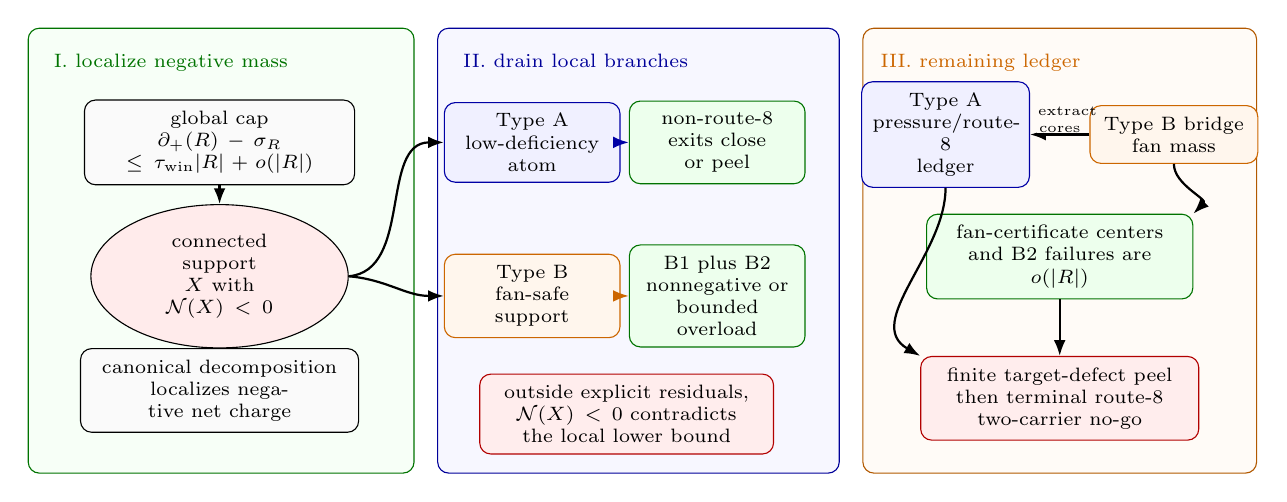
\begin{tikzpicture}[
supp/.style={ellipse,draw,fill=red!8,align=center,inner sep=3pt,text width=2.10cm},
box/.style={rectangle,rounded corners,draw,fill=black!2,align=center,inner sep=4pt,text width=2.55cm},
typea/.style={rectangle,rounded corners,draw=blue!65!black,fill=blue!6,align=center,inner sep=4pt,text width=2.55cm},
typeb/.style={rectangle,rounded corners,draw=orange!80!black,fill=orange!7,align=center,inner sep=4pt,text width=2.55cm},
good/.style={rectangle,rounded corners,draw=green!45!black,fill=green!7,align=center,inner sep=4pt,text width=2.55cm},
bad/.style={rectangle,rounded corners,draw=red!70!black,fill=red!7,align=center,inner sep=4pt,text width=2.55cm},
arr/.style={-{Latex[length=2mm]},thick},
dasharr/.style={-{Latex[length=2mm]},thick,dashed},
every node/.style={font=\scriptsize}
]
\draw[rounded corners,fill=green!3,draw=green!45!black] (-7.55,-3.10) rectangle (-2.65,2.55);
\draw[rounded corners,fill=blue!3,draw=blue!60!black] (-2.35,-3.10) rectangle (2.75,2.55);
\draw[rounded corners,fill=orange!3,draw=orange!70!black] (3.05,-3.10) rectangle (8.05,2.55);
\node[anchor=north west,green!45!black] at (-7.35,2.35) {I. localize negative mass};
\node[anchor=north west,blue!60!black] at (-2.15,2.35) {II. drain local branches};
\node[anchor=north west,orange!80!black] at (3.15,2.35) {III. remaining ledger};

\node[box,text width=3.15cm] (cap) at (-5.12,1.10) {global cap\\\(\defp(R)-\sigma_R\)\\\(\le\tau_{\rm win}|R|+o(|R|)\)};
\node[supp] (neg) at (-5.12,-0.60) {connected support\\\(X\) with\\\(\No(X)<0\)};
\node[box,text width=3.25cm] at (-5.12,-2.05) {canonical decomposition\\localizes negative net charge};
\draw[arr] (cap)--(neg);

\node[typea,text width=1.95cm] (ta) at (-1.15,1.10) {Type A\\low-deficiency\\atom};
\node[typeb,text width=1.95cm] (tb) at (-1.15,-0.85) {Type B\\fan-safe\\support};
\draw[arr] (neg.east) to[out=5,in=180] (ta.west);
\draw[arr] (neg.east) to[out=-5,in=180] (tb.west);
\node[good,text width=1.95cm] (aclosed) at (1.20,1.10) {non-route-8\\exits close\\or peel};
\node[good,text width=1.95cm] (bclosed) at (1.20,-0.85) {B1 plus B2\\nonnegative or\\bounded overload};
\draw[arr,blue!65!black] (ta)--(aclosed);
\draw[arr,orange!80!black] (tb)--(bclosed);
\node[bad,text width=3.45cm] at (0.05,-2.35) {outside explicit residuals,\\\(\No(X)<0\) contradicts\\the local lower bound};

\node[typea,text width=1.85cm] (route) at (4.10,1.20) {Type A\\pressure/route-8\\ledger};
\node[typeb,text width=1.85cm] (bridge) at (7.00,1.20) {Type B bridge\\fan mass};
\draw[arr] (bridge.west)--node[above,fill=orange!3,inner sep=0.5pt,font=\tiny,align=center,text width=0.55cm] {extract\\cores} (route.east);
\node[good,text width=3.10cm] (sub) at (5.55,-0.35) {fan-certificate centers\\and B2 failures are\\\(o(|R|)\)};
\draw[arr] (bridge.south) to[out=-90,in=45] (sub.north east);
\node[bad,text width=3.25cm] (final) at (5.55,-2.15) {finite target-defect peel\\then terminal route-8\\two-carrier no-go};
\draw[arr] (route.south) to[out=-90,in=150] (final.north west);
\draw[arr] (sub)--(final);
\end{tikzpicture}%
}
\caption[Visual proof of the branch-closure mass ledger]{Visual proof of the branch-closure mass ledger.  Panel I shows the large-budget cap localizing negative net charge to a connected admissible support \(X\) with \(\No(X)<0\).  Panel II shows the local branch drain used in \cref{thm:branch-kill}: Type A supports close through the non-route-8 exits or target-defect peeling, while Type B supports close through the B1 ledger together with B2, giving \(\No(X)\ge0\) outside the explicit residuals.  Panel III records the remaining global ledger.  Type B bridge and fan-mass residuals are charged to assigned surplus units and become \(o(|R|)\) after route-8 non-window cores are extracted into the Type A ledger.  The unified pressure ledger counts both target-defect and route-8 Type A entries.  Target-defect two-carrier entries are canonical exit-\textup{(4)} peel data, so finite descent removes them.  The terminal survivor would have to be a two-carrier route-8 obstruction, which is excluded by the carrier-reduction and no-go figures.}
\label{fig:branch-closure-mass-ledger}
\end{figure}

\paragraph{Framework branch table.}
The target-defect pressure section closes the remaining large-budget residual
by the following table.
\begin{longtable}{L{0.13\textwidth} L{0.19\textwidth} L{0.14\textwidth} L{0.14\textwidth} L{0.17\textwidth} L{0.17\textwidth}}
\FrameworkBranchTableHeader
Unified negative collection
&
A negative Type A support remains.
&
\(\delta(X)=-\No(X)\).
&
The unified Type A ledger.
&
The canonical decomposition.
&
\cref{def:typeA-unified-negative,lem:typeA-unified-deficit}.
\\
\addlinespace
Pressure ledger
&
Target-defect or route-8 entries remain.
&
Pressure units.
&
Boundary incidences.
&
The no-overcount pressure ledger.
&
\cref{lem:typeA-pressure-ledger-no-overcount}.
\\
\addlinespace
Open pressure
&
Boundary incidences do not pay all target-defect units.
&
Open pressure.
&
\(P_{13}\)-attachment accounting.
&
Same-window and primitive excess caps.
&
\cref{prop:typeA-exit4-closure-from-open-pressure,prop:typeA-exit4-closure-from-zero-shadow,prop:typeA-exit4-closure-from-window-blockers}.
\\
\addlinespace
Finite descent
&
An exit-\textup{(4)} peel is available.
&
One routed load.
&
The integer \(\Lambda_4\).
&
Strict decrease by one.
&
\cref{lem:typeA-pressure-is-exit4-peel,lem:typeA-exit4-finite-descent}.
\\
\addlinespace
Terminal route 8
&
No target-defect peel remains.
&
A two-carrier route-8 entry.
&
Deletion witnesses.
&
The canonical carrier core.
&
\cref{prop:typeA-route8-closure-from-nogo,thm:typeA-two-carrier-nogo}.
\\
\bottomrule
\end{longtable}


\appendix

\section{Finite curvature enumeration code}\label{app:curv-code}

This appendix reproduces the finite enumerations that certify the constants used above.  Each listing is self-contained and was run under CPython~3 (standard library, with \texttt{numpy} for the second block); the displayed output immediately below each listing is the certificate.  The first block certifies the legal-label count $|\labels|=399$ of \cref{lem:labels} together with the two-step curvature counts $543958,\,432672,\,111286$ of \cref{lem:curv-enum}, and hence the value of $c_\Omega$.

\begin{lstlisting}[language=Python]
from itertools import combinations
from collections import Counter
import math

labels=[]
for mask in range(1,1<<13):
    S=[i for i in range(13) if (mask>>i)&1]
    ok=True
    for a,b in combinations(S,2):
        if abs(a-b) in (2,6):
            ok=False
            break
    if ok:
        labels.append(tuple(S))

print(len(labels))
print(Counter(map(len,labels)))

powers={2**k for k in range(2,20)}

def C(s,S,T):
    return all(s+2+abs(i-j) not in powers for i in S for j in T)

W=0
pos=0
flat=0
for S in labels:
    for A in labels:
        if not C(1,S,A):
            continue
        for T in labels:
            if not C(1,A,T):
                continue
            W+=1
            if not C(2,S,T):
                pos+=1
            else:
                flat+=1

print(W,pos,flat)
print(pos/W, flat/W, math.log2(W/flat))
\end{lstlisting}

The output is:
\begin{lstlisting}
399
Counter({3: 122, 4: 122, 5: 63, 2: 60, 6: 17, 1: 13, 7: 2})
543958 432672 111286
0.7954143518433409 0.20458564815665917 2.28922315244071
\end{lstlisting}

The second block certifies the constant
\[
 c_{13}=118.108581006\ldots
\]
used in \cref{lem:p13-window-package,prop:p13-density}, as the sum of the
$91$ finite curvature barriers; it uses matrix multiplication to avoid an
explicit $399^3\cdot91$ loop.

\begin{lstlisting}[language=Python]
from itertools import combinations
import numpy as np, math

L=[]
for mask in range(1,1<<13):
    inds=[i for i in range(13) if (mask>>i)&1]
    ok=True
    for a,b in combinations(inds,2):
        if abs(a-b) in (2,6):
            ok=False
            break
    if ok:
        L.append(mask)
assert len(L)==399

def indices(mask):
    return [i for i in range(13) if (mask>>i)&1]

Ms=[]
for s in range(15):
    forb={2**r-s-2 for r in range(2,20) if 0 <= 2**r-s-2 <= 12}
    M=np.ones((len(L),len(L)), dtype=np.int8)
    for i,S in enumerate(L):
        Si=indices(S)
        for j,T in enumerate(L):
            Tj=indices(T)
            bad=any(abs(a-b) in forb for a in Si for b in Tj)
            if bad:
                M[i,j]=0
    Ms.append(M)

total=0.0
vals=[]
for a in range(1,15):
    for b in range(1,15-a): # a,b >= 1 and a+b <= 14
        middle_counts=Ms[a].astype(np.int32) @ Ms[b].astype(np.int32)
        W=int(middle_counts.sum())
        bad=int((middle_counts*(1-Ms[a+b])).sum())
        flat=W-bad
        val=math.log2(W/flat)
        vals.append((a,b,W,bad,flat,val))
        total += val

print(len(vals))
print(total)
print(min(vals, key=lambda x: x[-1]))
\end{lstlisting}

The output is:
\begin{lstlisting}
91
118.10858100609198
(4, 4, 6648206, 1190878, 5457328, 0.284770329720...)
\end{lstlisting}

The third block reproduces the Type B fan constants used in
\cref{rem:fan-finite} and \cref{lem:typeB-exclusion}.  The proof of those
constants is the structural label-packing argument in
\cref{lem:fan-certificate}.  The listing builds the same graph on the $399$
labels with adjacency relation $C_2(S,T)=1$, computes its clique number, and
computes the marked variant corresponding to the non-singleton-label cap.  The
residual class in \cref{def:typeB-multiclosed-residual} is determined by the
positive closed-neighbour deficit $D_B>0$: for $k\le7$ this means at least two
cubic-closed neighbours, while for $k=8$ it also includes the single
cubic-closed border case.

\begin{lstlisting}[language=Python]
from fractions import Fraction
from itertools import combinations

labels=[]
for mask in range(1,1<<13):
    S=tuple(i for i in range(13) if (mask>>i)&1)
    if all(abs(a-b) not in (2,6) for a,b in combinations(S,2)):
        labels.append(S)

powers={2**k for k in range(2,20)}

def C(s,S,T):
    return all(s+2+abs(i-j) not in powers for i in S for j in T)

n=len(labels)
adj=[0]*n
edges=0
for i,S in enumerate(labels):
    for j in range(i+1,n):
        if C(2,S,labels[j]):
            adj[i] |= 1<<j
            adj[j] |= 1<<i
            edges += 1

def maximum_clique(mask):
    best_size=0
    best_bits=0
    def color_sort(P):
        verts=[]
        colors=[]
        U=P
        color=0
        while U:
            color += 1
            Q=U
            while Q:
                bit=Q & -Q
                v=bit.bit_length()-1
                verts.append(v)
                colors.append(color)
                U &= ~bit
                Q &= ~bit
                Q &= ~adj[v]
        return verts, colors
    def expand(size,bits,P):
        nonlocal best_size,best_bits
        if not P:
            if size > best_size:
                best_size=size
                best_bits=bits
            return
        verts,colors=color_sort(P)
        for idx in range(len(verts)-1,-1,-1):
            if size + colors[idx] <= best_size:
                return
            v=verts[idx]
            bit=1<<v
            if P & bit:
                expand(size+1,bits|bit,P & adj[v])
                P &= ~bit
                if size + P.bit_count() <= best_size:
                    return
    expand(0,0,mask)
    return best_size,best_bits

omega,wit=maximum_clique((1<<n)-1)
omega_ns=0
wit_ns=0
for i,S in enumerate(labels):
    if len(S) >= 2:
        size,bits=maximum_clique(adj[i] | (1<<i))
        if size > omega_ns:
            omega_ns=size
            wit_ns=bits

def bit_labels(bits):
    return [labels[i] for i in range(n) if (bits>>i)&1]

simple_charge_k_le_7=min(
    (Fraction(3-k,1)-Fraction(1,4)-Fraction(1,4)
     + Fraction(3,4)*(k-1), k)
    for k in range(4,8)
)
charge_k8_no_closed=Fraction(3-8,1)-Fraction(1,4)+8*Fraction(3,4)

print('labels', n)
print('fan_safe_edges', edges)
print('omega_C2', omega)
print('omega_C2_witness', bit_labels(wit))
print('omega_with_nonsingleton', omega_ns)
print('nonsingleton_witness', bit_labels(wit_ns))
print('simple_charge_k_le_7', simple_charge_k_le_7[0], 'at_k',
      simple_charge_k_le_7[1])
print('charge_k8_no_closed', charge_k8_no_closed)
\end{lstlisting}

The output is:
\begin{lstlisting}
labels 399
fan_safe_edges 18301
omega_C2 8
omega_C2_witness [(1,), (2,), (3,), (4,), (9,), (10,), (11,), (12,)]
omega_with_nonsingleton 7
nonsingleton_witness [(0, 1), (2,), (3,), (8,), (9,), (10,), (11,)]
simple_charge_k_le_7 0 at_k 7
charge_k8_no_closed 3/4
\end{lstlisting}

\begin{remark}[Fan-packing reproducibility check]\label[remark]{rem:fan-packing-reproducibility}
The fan-packing bound used in the Type B proof is established structurally in
\cref{lem:fan-certificate}.  The listing above is retained only as a
reproducibility check of the same constants for the $399$-label graph; it is
not an additional premise in the proof.
\end{remark}

\paragraph{Framework branch table.}
The enumeration appendix is a computational-certificate register.  Each row
states which finite datum is exported and where the proof consumes it.
\begin{longtable}{L{0.13\textwidth} L{0.19\textwidth} L{0.14\textwidth} L{0.14\textwidth} L{0.17\textwidth} L{0.17\textwidth}}
\FrameworkBranchTableHeader
Legal-label certificate
&
All subsets of \(\{0,\ldots,12\}\) are tested for forbidden gaps.
&
\(|\labels|=399\) and the size distribution.
&
The finite subset enumeration.
&
The predicate in the code is the predicate in \cref{lem:labels}.
&
Consumed by \cref{lem:labels}.
\\
\addlinespace
Curvature certificate
&
All ordered legal-label triples are tested.
&
\(\begin{gathered}543958,\\432672,\\111286\end{gathered}\).
&
The finite curvature tensor.
&
The code applies \(C_1,C_2\) exactly as defined in the text.
&
Consumed by \cref{lem:curv-enum}.
\\
\addlinespace
Window-package rate
&
All \(91\) pairs \(a,b\ge1\), \(a+b\le14\), are summed.
&
\(c_{13}\).
&
The matrix-computed barrier list.
&
The printed count \(91\) verifies that every scale pair is included once.
&
Consumed by \cref{lem:p13-window-package,prop:p13-density}.
\\
\addlinespace
Type B reproducibility
&
The \(399\)-label fan graph is checked independently.
&
Clique and marked-clique constants.
&
The structural proof of \cref{lem:fan-certificate}.
&
The code is a reproducibility check, not a separate premise.
&
Checks \cref{rem:fan-finite,lem:typeB-exclusion}.
\\
\bottomrule
\end{longtable}

\clearpage
\section{Proof resilience: residual counterexamples under lemma failure}\label{app:resilience}

For every \emph{closing cell} (terminal node) of the proof-dependency diagram, this appendix records what survives if that cell's closing lemma is \emph{false} and no redundancy covers it.  The entry is the forced structure of a hypothetical minimal counterexample confined to that cell---that is, the reduction theorem the proof degrades into at that leaf.  The logic is that a closing lemma does not merely delete a possibility when it fails; its negation is a structural hypothesis.  A surviving counterexample must satisfy \emph{all standing invariants accumulated up to that node} (it does not lose them) \emph{together with} the negation of the failed lemma's conclusion.  Thus every degradation cell is a specified residual problem, not an unconstrained failure mode.

Notation is as in the manuscript: $G$ is the minimal counterexample, $\delta(G)\ge3$, $R$ is the $P_{13}$-free remainder, $\theta=p_{13}/n$, $\defp(X)=\sum_v\max(0,3-d_X(v))$, $\sigma(X)=\sum_v\max(0,d_G(v)-3)$, $\No(X)=\defp(X)-\sigma(X)-\tfrac14|V(X)|$, $W_2$ is the two-step curvature supply, $c_\Omega$ the flatness entropy cost, and $\beta=m-n+1$.  ``Standing invariants'' are the invariants established at earlier-or-equal nodes; they are retained in every residual cell below.

\paragraph{Framework branch table.}
The resilience appendix already gives the detailed degradation rows below; the
framework branch table for the appendix is the following compact index.
\begin{longtable}{L{0.13\textwidth} L{0.19\textwidth} L{0.14\textwidth} L{0.14\textwidth} L{0.17\textwidth} L{0.17\textwidth}}
\FrameworkBranchTableHeader
Covered leaf
&
A listed closure is removed but a redundant route remains.
&
The residual cell.
&
The redundant closure.
&
The standing invariant set.
&
Recorded as covered in the detailed tables.
\\
\addlinespace
Dense-window auxiliary
&
The window entropy branch degrades to dense-window blocks.
&
Quiet-block demand.
&
The target-compatible external input.
&
Canonical block boundaries.
&
\cref{lem:app-dense-window-closure}.
\\
\addlinespace
Global smearing
&
The rank-drop branch degrades to a whole-graph dependence.
&
Closed exact-profile data.
&
Minimality or label-injectivity.
&
The empty-boundary profile.
&
\cref{lem:app-global-smearing-closure}.
\\
\addlinespace
Type A failure
&
The route-8 or exit-\textup{(4)} closure is weakened.
&
Terminal carrier package.
&
The carrier ledger.
&
Declared witnesses.
&
\cref{lem:app-typeA-quiet-bound}.
\\
\addlinespace
Type B failure
&
The fan ledger or B2 closure is weakened.
&
Bridge or overlap residual.
&
The fan-mass ledger.
&
Assigned surplus.
&
\cref{rem:app-typeB-finite-only}.
\\
\bottomrule
\end{longtable}

\paragraph{How to read a row.}
{\small
\begin{longtable}{L{0.22\textwidth} L{0.70\textwidth}}
\toprule
\textbf{Column} & \textbf{Meaning} \\
\midrule
\endhead
Node & Terminal node id $[k]$ from the diagram, with tikz id. \\
Closing lemma & The single labeled result that discharges this leaf. \\
Closing condition & The inequality or identity whose truth closes the leaf. \\
Slack & Margin by which it currently closes (how wrong the constant can be). \\
Redundant cover? & Whether another standing route re-closes this cell if the lemma fails. \\
Residual counterexample & Forced structure of a surviving $G$ if the lemma is false and no cover applies. \\
\bottomrule
\end{longtable}
}

\paragraph{A. Trivial / external-input leaves.}
These do not degrade to nontrivial residual reductions: their negation is either a direct cycle (so $G$ is not a counterexample at all) or a failure of an external theorem, not of this proof.

{\scriptsize\setlength{\tabcolsep}{3pt}
\begin{longtable}{L{0.09\textwidth} L{0.095\textwidth} L{0.15\textwidth} L{0.08\textwidth} L{0.105\textwidth} L{0.335\textwidth}}
\toprule
\textbf{Node} & \textbf{Closing lemma} & \textbf{Closing condition} & \textbf{Slack} & \textbf{Redundant cover?} & \textbf{Residual counterexample (if false)} \\
\midrule
\endhead
{[3]} \texttt{notbad} & def.\ of counterexample & $\delta(G)\ge3$ and no $C_{2^j}$ & exact (definitional) & --- & None --- if it fails, $G$ already has a power-of-two cycle (not a counterexample). \\
{[7]} \texttt{cycle} & \cref{lem:return-equivalence} & a Mersenne return $\iff$ a $2^k$ cycle & exact (arithmetic identity) & --- & None --- failure means the return/cycle dictionary is misstated; $G$ would have a $2^k$ cycle. Pure bookkeeping. \\
{[16]} \texttt{hss} & \cref{thm:p13free} (HSS, external) & $P_{13}$-free $+\ \delta\ge3\ \Rightarrow 2^k$ cycle & external & --- & Not this proof's leaf. The proof uses the Hegde--Sandeep--Shashank theorem as its black-box external input; if that theorem is unavailable, the window/remainder spine has no entry point. \\
\bottomrule
\end{longtable}
}

\paragraph{B. Density / supply leaves (close by counting; degrade to ``dense-window'' reductions).}
{\scriptsize\setlength{\tabcolsep}{3pt}
\begin{longtable}{L{0.09\textwidth} L{0.095\textwidth} L{0.15\textwidth} L{0.08\textwidth} L{0.105\textwidth} L{0.335\textwidth}}
\toprule
\textbf{Node} & \textbf{Closing lemma} & \textbf{Closing condition} & \textbf{Slack} & \textbf{Redundant cover?} & \textbf{Residual counterexample (if false, no cover)} \\
\midrule
\endhead
{[23]} \texttt{overflow} & \cref{prop:p13-density} via \cref{eq:feasibility} & $\theta\le0.011985$ (else window entropy $>$ skeleton budget) & feasibility gap $0.1+116.8\theta\le1.5$; binds only at $\theta\approx0.012$ & \textbf{Target-compatible auxiliary closure.} The dense correlated-window residual is closed in \cref{lem:app-dense-window-closure} by the stated quiet-block input. & $G$ has a \emph{dense induced-$P_{13}$ packing}: $\theta>0.011985$, so the maximal disjoint packing covers $>15.6\%$ of vertices, yet the window entropy still fits under the skeleton budget. The target-compatible auxiliary closure shows that such entropy-cheap density must either create close cycle lengths in a dyadic-safe atom or pay quadratic boundary, in both cases restoring a contradiction. \\
{[29]}\,$\to$\,{[28]} \texttt{stub} & \cref{lem:stub-positive} & each induced $P_{13}$ exports $\le15+\sigma(P)$ incidences & exact ($12$-edge identity); only $\theta$ feeds the normalized form & \textbf{Framework-independent.} Uses only $\delta\ge3$, ``induced $P_{13}$ has $12$ edges'', and disjointness. & If the constant $15$ were miscounted, the residual $G$ would be one whose remainder borrows more than $15$ incidences per window, contradicting the induced-path edge count. Thus failure here is a numerical misstatement of the incidence identity, not a new graph-theoretic residual. \\
\bottomrule
\end{longtable}
}

\paragraph{C. Curvature / rank leaves (close by supply-vs-demand; degrade to ``flat-remainder'' reductions).}
{\scriptsize\setlength{\tabcolsep}{3pt}
\begin{longtable}{L{0.09\textwidth} L{0.095\textwidth} L{0.15\textwidth} L{0.08\textwidth} L{0.105\textwidth} L{0.335\textwidth}}
\toprule
\textbf{Node} & \textbf{Closing lemma} & \textbf{Closing condition} & \textbf{Slack} & \textbf{Redundant cover?} & \textbf{Residual counterexample (if false, no cover)} \\
\midrule
\endhead
{[30]} \texttt{wedge} (demand floor) & \cref{lem:wedge-lower} & under \cref{def:near-cubic-spine}, $W_2(R)\ge2.543\cdot|R|$; high entropy gives $2.574\cdot|R|$ & \textbf{$4.1\times$ over the $0.611$ supply cap} & \textbf{Yes inside the near-cubic spine.} The net-charge collision (diagram node {[60]}, $0.25$ vs $0.2282$) reaches a contradiction without the curvature magnitude; \cref{rem:closure-robust} states closure already holds from the window-only cap. & $G$ has a \emph{curvature-poor remainder}: $W_2(R)<2.543\cdot|R|$, i.e.\ the $P_{13}$-free remainder admits fewer than $2.543$ two-step curvature tests per vertex. With the standing invariants (empty $3$-core, deficiency $\le0.2282$) this forces an unusually \emph{flat} atom remainder---locally tree-like wedge structure avoiding curvature-positive triples. \emph{Reduction:} ``a counterexample's remainder is curvature-flat below density $2.543$; classify flat $P_{13}$-free atoms.'' Recoverable via the net-charge route, which does not consume the wedge magnitude. \\
{[32]}/{[47]} \texttt{fullrank} & \cref{lem:full-rank} & $r_\Omega(R)\ge W_2-o(|R|)$ (no rank drop) & absorbs $o(|R|)$; rank-drop branch~D separately closes at {[46]} & \textbf{Yes.} Branch~D (\cref{lem:no-silent-global-smearing}, inv 34/35) independently closes the rank-drop case; the two-budget split also re-routes. & $G$ has a \emph{rank-deficient curvature operator}: $r_\Omega(R)<W_2-\Omega(|R|)$, so a linear fraction of curvature tests are dependent. The proper-support cases are routed to target defect, compression, or proper smearing. The whole-graph case is closed by the exact closed response profile: empty context does not identify labelled curvature coordinates, and a non-injective closed quotient must produce a smaller closed counterexample. \\
{[45]} \texttt{globalterm} & \cref{lem:no-silent-global-smearing} & no silent global delocalization of dyadic support & qualitative (closed exactness is label-injective on raw curvature tests) & \textbf{Closed in the main text.} \cref{lem:app-global-smearing-closure} records the corresponding degradation-cell closure. & A surviving row {[45]} residual would require a target-complete whole-graph quotient of $\rho_\varnothing^{\rm ex}(G)$ that is not label-injective on raw curvature tests and has no smaller closed representative. This contradicts \cref{def:admissible-rank-quotient,lem:no-silent-global-smearing}. \\
{[50]}/{[54]} \texttt{entcap} & \cref{prop:entropy-high-theta} / \cref{prop:two-budget} & high-$\theta$ branch: entropy cap $c_\Omega\cdot\mathrm{rank}$ exceeds budget when the rank input is available & routing is exhaustive; only the high-entropy and repetitive low-entropy subcases add new rank/entropy information & \textbf{Partial routing.} The nonrepetitive low-entropy subcase is deliberately passed to the large-budget net-charge analysis, not closed here. & $G$ sits in a \emph{nonrepetitive low-entropy regime}: $\eta(R)<\tfrac1{10}\log_2 n$ per vertex, the radius-$2$ type coordinate has linear bit-content, and the local-type dominance lemma does not apply.  \emph{Reduction:} this branch carries no extra curvature closure claim and is handled only by the later net-charge/local-residual analysis. \\
\bottomrule
\end{longtable}
}

\paragraph{D. Net-charge terminus leaves (close by discharging; degrade to ``charged-atom'' reductions).}
{\scriptsize\setlength{\tabcolsep}{3pt}
\begin{longtable}{L{0.09\textwidth} L{0.095\textwidth} L{0.15\textwidth} L{0.08\textwidth} L{0.105\textwidth} L{0.335\textwidth}}
\toprule
\textbf{Node} & \textbf{Closing lemma} & \textbf{Closing condition} & \textbf{Slack} & \textbf{Redundant cover?} & \textbf{Residual counterexample (if false, no cover)} \\
\midrule
\endhead
{[60]} \texttt{contrad} & \cref{prop:negative-net-charge} $+$ \cref{lem:netcharge-superadd} & $\tfrac14|R|\le\defp(R)-\sigma(R)=\defp(R)-\sigma_R\le\tau_{\rm win}|R|+o(|R|)$ with $\tau_{\rm win}<\tfrac14$ & $\sim9.6\%$ ($0.25$ vs $0.2282$ per $|R|$) & \textbf{Yes.} The second independent collision form; the curvature route ({[30]}) reaches a contradiction on its own with large slack. & $G$ has a \emph{net-charge-negative residual that does not localize}: $\defp(R)-\sigma(R)<\tfrac14|R|$ globally, yet net charge fails to concentrate on a connected support (superadditivity localization fails). \emph{Reduction:} ``a counterexample distributes a $\tfrac14$-deficit across $R$ with $\No(X)\ge0$ on every connected piece''---forbids the very cell-wise accounting the discharging needs; isolates a precise superadditivity gap to repair. \\
{[91]} \texttt{atomthm} (Type A, $\sigma=0$) & \cref{lem:typeA-exclusion} via \cref{lem:typeA-threshold-algebra,lem:typeA-exit4-peeling-charge,lem:typeA-unpeeled-visible-routing,lem:typeA-unpeeled-silent-routing,lem:typeA-exit4-residual-routing,lem:typeA-exit4-discharge,lem:typeA-saturated-handoff,lem:typeA-unsaturated-discharge} & outside target-defect peeling, route 8, and the Type B handoff, $\defp(X)\ge\tfrac14|V(X)|\iff 2|E(X)|/|V(X)|\le2.75$, so $\No(X)\ge0$ & raw thresholds $H_0\le4$, $H_1\le8$, $H_2\le12$; exits 1--3, 5, and 6 close; exit 4 peels one target-defective routed load with exact \(1/4\) receiver-charge accounting; exit 7 hands off to Type B; then unsaturated discharging $11n_0+7n_1+3n_2\ge n_3$ & \textbf{Local split.} The $4/8/12$ saturated cases in exits 1--3, 5, and 6 are removed by target, compression, and delocalization, while exit 4 removes its supported target-defective load before the $3/7/11$ charge calculation.  Exit 7 is represented by Type B, and route 8 is the reduced silent trace-basin branch of \cref{def:typeA-silent-core-residual}. & $G$ would contain a \emph{dense low-deficiency admissible atom}: a connected, $\sigma=0$, empty-$3$-core, $P_{13}$-free support with average degree $>2.75$.  The Type A split sends exits 1--3, 5, and 6 to closed contradictions, exit 4 to target-defect peeling, exit 7 to Type B, and the remaining unsaturated case to discharging; if the route-8 branch carries the large-budget Type A deficit, the declared $u$-supported response algebra and canonical minimal target-complete carrier cores reduce it to a two-carrier route-8 residual, with quiet-block boundedness recorded in \cref{lem:app-typeA-quiet-bound}. \\
{[74]} \texttt{fanthm} (Type B, $\sigma>0$) & \cref{lem:typeB-exclusion} and \cref{prop:typeB-bridge-sublinear} via \cref{def:marked-typeB-fan}, \cref{def:typeB-window-incidence-profile}, \cref{def:typeB-hybrid-incidence}, \cref{def:closed-fan-window-pair}, \cref{def:direct-cycle-free-closed-pair}, \cref{lem:typeB-direct-fan-window-cycles}, \cref{lem:typeB-two-window-cycles}, \cref{lem:typeB-multiclosed-budget}, \cref{lem:typeB-hybrid-incidence-budget}, \cref{lem:typeB-hybrid-B1}, \cref{def:typeB-ledger-carriers}, \cref{def:typeB-candidate-ledger}, \cref{def:typeB-overlap-obstruction}, \cref{lem:typeB-bridge-to-overlap}, \cref{lem:typeB-global-local-reflection}, \cref{prop:typeB-global-local-bridge}, \cref{def:typeB-bridge-statements}, \cref{prop:typeB-bridge-reduction}, \cref{def:typeB-multiclosed-residual}, \cref{def:typeB-residual-mass}, \cref{lem:typeB-processed-boundary-bound}, \cref{lem:decorated-envelope-with-route8-core}, \cref{lem:typeB-bridge-deficit-bound}, \cref{lem:typeB-bridge-with-route8-core}, \cref{rem:fan-finite}, and \cref{lem:fan-certificate} & outside route 8, outside fan-certificate residual centers, and outside B2 failure, every certificate-marked fan has $d_G(h)\le8$, every nonpositive-deficit marked fan has nonnegative closed-neighbourhood charge, every positive-deficit fan has the local hybrid B1 incidence ledger, and B2 supplies the disjoint ledger needed to sum the fans; in the near-cubic spine, residual centers and B2 failures satisfy $M_B\le416\sigma(G)=o(|R|)$ after any route-8 non-window core is extracted into $D_A$ and grouped-envelope centers are counted at most twice & certificate-closed iff $D_B\le0$; every positive-deficit residual has $D_B=c-\tfrac{11-k}{4}$ paid by half-credit on the $2c$ disjoint non-$h$ incidences, split into window credit $I_W/2$ and non-window demand $D_N$; each bridge residual is charged by at most 208 times its assigned surplus plus the extracted route-8 Type A deficit & \textbf{Structural reduction to B2 plus fan-mass closure.} Direct fan-window and two-window cycles close by explicit path construction; local B1 is the hybrid incidence budget; every disjoint-carrier B2 failure is represented by a minimal overlap obstruction carrying contextual dyadic safety, window-stub capacity, replacement/delocalization routing, and a sublinear fan-mass budget in the near-cubic spine after route-8 cores are charged to $D_A$; fan-certificate residual centers and grouped envelopes enter this fan-mass bound directly. & In the near-cubic spine, a surviving Type B bridge obstruction has only sublinear bridge mass outside the Type A pressure/route-8 ledger, so it cannot carry the linear large-budget obstruction without entering node {[123]}. \\
{[76]}/{[85]} \texttt{branch} (local closures) & \cref{thm:branch-kill} & combines {[30]}$+${[60]}$+$entropy: outside explicit Type A target-defect/route-8 and Type B bridge residuals, the entropy-admissible branch has no survivor & inherits the available component slacks: about $4.1\times$ in the curvature form and about $9.6\%$ in the net-charge form; Type B bridge mass is $o(|R|)$ after route-8 cores are extracted into the Type A ledger & \textbf{Local join.} It leaves only the explicit Type A pressure/route-8 ledger for node {[123]}. & $G$ \emph{survives the branch squeeze} only if the negative local support contributes to the explicit Type A pressure/route-8 ledger; Type B fan-certificate residual centers and B2 failures are too small in total to carry the required linear deficit. \\
{[123]} \texttt{closed} (pressure descent) & \cref{thm:large-budget-route8-only} & after the branch-kill reduction, the remaining large-budget Type A target-defect/route-8 ledger either peels a target-defect load by exit \textup{(4)} or forces a two-carrier route-8 entry & inherits the unified burden lower bound, the pressure no-overcount ledger, finite descent of \(\Lambda_4\), the route-8 burden lower bound, and the private-carrier upper bound; Type B bridge mass has already been removed at {[76]}/{[85]} & \textbf{Join node feeding the terminal no-go.} Target-defect two-carrier entries decrease \(\Lambda_4\); the terminal non-peeling case enters node {[124]}, which is discharged by carrier deletion. & $G$ can survive node {[123]} only if the finite exit-\textup{(4)} descent has terminated and the remaining entry is the terminal two-carrier route-8 obstruction through the canonical carrier-core ledger. \\
{[124]} \texttt{nogo} (two-carrier route 8) & \cref{def:typeA-true-route8-residual,lem:typeA-deletion-witness-declared,lem:typeA-two-carrier-deletion-canonical,lem:typeA-carrier-deletion-exit,thm:typeA-two-carrier-nogo}, with \cref{def:typeA-terminal-two-carrier,prop:typeA-route8-closure-from-nogo} & no terminal two-carrier route-8 obstruction exists & inherits the route-8 lower bound, the private-carrier upper bound, cut parity, declared deletion witnesses, and all absent-exit constraints & \textbf{Terminal local no-go.} In a two-carrier entry, declared essential deletion witnesses first give canonical exit-(4) quotients and then realize exit (4), which is absent in a true route-8 residual. & A false instance is exactly a terminal two-carrier route-8 obstruction: a true route-8 entry with at least two essential carriers, at most two private essential carriers, and declared carrier-deletion witnesses for every essential carrier. \\
\bottomrule
\end{longtable}
}

\begin{remark}[Tight margin in the route-8 carrier reduction]\label[remark]{rem:route8-carrier-margin}
The private-carrier reduction at node {[123]} uses the numerical inequality
\[
12\left(\frac14-\tau_{\rm win}\right)>\tau_{\rm win},
\qquad\text{equivalently}\qquad
\tau_{\rm win}<\frac3{13}.
\]
With the printed constants, \(\tau_{\rm win}=0.22817486846\ldots\), while
\(3/13=0.23076923076\ldots\).  The relative margin is therefore about
\[
\frac{3/13-\tau_{\rm win}}{3/13}=0.01124\ldots .
\]
This is the tight carrier-reduction margin.  Any later argument that spends
additional boundary-incidence or stub capacity before
\cref{prop:typeA-route8-carrier-reduction} must recheck this inequality.
\end{remark}

\paragraph{External-input closures for partial degradation cells.}
The next three lemmas use target-compatible forms of the auxiliary external
inputs listed in the constraint ledger.  The named external theorems supply the
graph-theoretic alternatives; the target-compatible clauses below state exactly
how those alternatives interact with the Mersenne-return algebra and the
canonical support ledger of this paper.  Thus no closure below depends on an
unstated propagation step.  For a connected support $Y$, write
$b(Y)=|\partial Y|$ for its boundary size in the ambient counterexample.

\begin{lemma}[Dense-window residual closes by quiet-block input]\label[lemma]{lem:app-dense-window-closure}
Assume the following target-compatible Bondy--Vince/Gao--Ma input for the
canonical blocks generated by a row {[23]} dense-window residual.
\begin{enumerate}[label=(\alph*), leftmargin=2.2em]
\item Each canonical block $Y$ is almost cubic, and its sub-cubic vertices are
boundary vertices charged to the packed-window incidence ledger of
\cref{lem:stub-positive}.
\item If $Y$ exports two cycle lengths differing by $1$ or $2$, then the
corresponding two edge-rooted returns lie in one boundary fibre and force either
a return length in $\Mers$ or a target-complete replacement in the sense of
\cref{lem:replacement}.
\item If $Y$ is quiet, then $|Y|<5b(Y)^2$, and the canonical quiet blocks are
boundary-disjoint up to packed-window interfaces; summing their boundary
charges restores the feasibility inequality \cref{eq:feasibility}.
\end{enumerate}
Then the dense-window residual in row {[23]} is empty.
\end{lemma}

\begin{proof}
Suppose row {[23]} survives.  Then the maximal induced-$P_{13}$ packing has
$\theta>0.011985$, while the corresponding window states remain below the
skeleton entropy bound.  Apply the target-compatible input to the canonical
blocks of this residual.  In the exported-length alternative, clause (b) gives a
Mersenne return or a target-complete replacement.  The first contradicts
\cref{lem:return-equivalence}; the second contradicts minimality through
\cref{lem:replacement}.  In the quiet alternative, clause (c) restores
\cref{eq:feasibility}, contradicting $\theta>0.011985$ in the entropy-cheap
dense-window branch.  The two alternatives exhaust the input, so row {[23]} is
empty.
\end{proof}

\begin{lemma}[Global smearing closure]\label[lemma]{lem:app-global-smearing-closure}
The rank-one global-mode residual in row {[45]} is empty.
\end{lemma}

\begin{proof}
Let a row {[45]} residual survive.  By
\cref{lem:no-silent-global-smearing}, the corresponding global dependence
is target-defective, has a strictly smaller admissible closed representative, or
contributes exact label-injective global response data.  The first
alternative cannot witness a target-dependence by
\cref{def:curvature-target-dependence}; the second contradicts the
lexicographic minimality of \(G\); and the third supplies no rank reduction of
$r_\Omega(R)$ by \cref{def:exact-response-profile,def:admissible-rank-quotient}.
This contradicts the definition of a row {[45]} rank-one global-mode residual.
Hence row {[45]} is empty.
\end{proof}

\begin{lemma}[Route-8 Type A residual is bounded by quiet-block input]\label[lemma]{lem:app-typeA-quiet-bound}
Assume the following target-compatible Bondy--Vince/Gao--Ma input for route-8
Type A supports.
\begin{enumerate}[label=(\alph*), leftmargin=2.2em]
\item Every maximal almost-cubic block of a route-8 Type A support either
exports two cycle lengths differing by $1$ or $2$, or is quiet and satisfies
$|Y|<5b(Y)^2$.
\item In the exported-length alternative, completion through the ambient
boundary gives a Mersenne return or a target-complete replacement.
\item If all maximal blocks are quiet, gluing them along the canonical boundary
of the Type A support gives $|X|<5b(X)^2$.
\end{enumerate}
Then every admissible silent-core residual profile of
\cref{def:typeA-silent-core-residual} lies in a finite boundary-labelled
residual class determined by
\[
|X|\le6142,\qquad |X|<5b(X)^2,
\]
with all boundary return profiles avoiding $\Mers$.
\end{lemma}

\begin{proof}
Let $X$ be the Type A support underlying an admissible silent-core residual
profile.  It is connected, subcubic,
$P_{13}$-free, has empty internal $3$-core, satisfies $\sigma(X)=0$, and has
$\defp(X)<|X|/4$.  The $P_{13}$-free diameter argument in the Type A analysis
already gives $|X|\le6142$.

Apply the Bondy--Vince/Gao--Ma input to every maximal almost-cubic block of
$X$.  If one of them realizes the exported-length alternative, clause (b)
creates a Mersenne return or a target-complete replacement, both forbidden in an
admissible support.  Hence every maximal block is quiet.  Clause (c) gives
$|X|<5b(X)^2$.  Since $|X|\le6142$ and the boundary labels are drawn from the
finite $399$-label $P_{13}$ algebra, only finitely many boundary-labelled return
profiles remain.  Thus the auxiliary input bounds route 8 by a finite
boundary-labelled residual class with explicit Mersenne-avoiding return
profiles; it does not by itself close that residual.
\end{proof}

\begin{remark}[Type B residual after the structural fan-window reduction]\label[remark]{rem:app-typeB-finite-only}
The unused external inputs do not close node {[74]}; the available closure is the
structural label-packing lemma recorded in \cref{lem:fan-certificate}.
Bondy--Vince/Gao--Ma controls quiet almost-cubic blocks, and Kleitman--West
controls global tree--cotree profiles; the Type B obstruction is a local
fan-safe clique around a high-degree surplus vertex.  The packing lemma proves
the $C_2$ clique cap, the marked non-singleton cap, and the spectral bound
$d_G(h)\le\rho(A(\Fsafe_h))+1$ for certificate-marked fans, and it discharges
certificate-closed marked fans.  Fan-certificate residual centers are charged
directly to their assigned surplus units.  The structural fan-window reduction of
\cref{lem:typeB-direct-fan-window-cycles,lem:typeB-two-window-cycles,lem:typeB-multiclosed-budget,lem:typeB-hybrid-incidence-budget,lem:typeB-hybrid-B1}
then removes every positive-deficit pair that already contains a direct dyadic
cycle and pays every remaining positive-deficit fan by hybrid half-credit on
its window and non-window incidences.  The refined support ledger B2 is the
local disjointness statement needed to sum those fan entries.  By
\cref{lem:typeB-bridge-to-overlap,lem:typeB-global-local-reflection}, any
disjoint-carrier failure of that bridge ledger is represented by a minimal
overlap obstruction carrying contextual dyadic safety, high-degree separation,
window compatibility, replacement routing, and minimal-overlap constraints.  The
fan-mass closure
\cref{def:typeB-residual-mass,lem:typeB-bridge-deficit-bound,lem:typeB-bridge-with-route8-core,prop:typeB-bridge-sublinear}
charges fan-certificate residual centers and disjoint-carrier failures to their
assigned surplus units and gives total negative Type B bridge mass
$O(\sigma(G))=o(|R|)$.  Thus neither Type B residual form is a terminal
large-budget residual.
\end{remark}

\paragraph{Summary: the degradation ladder.}
Ordered by how much the proof loses if that single leaf fails with no redundant cover:
\begin{enumerate}[label=\arabic*., leftmargin=1.8em]
\item \textbf{Definitional or exact-counting leaves:} {[29]} \texttt{stub} --- framework-independent counting; {[3]}/{[7]} definitional.
\item \textbf{Redundantly covered or routed forward:} {[30]} curvature demand (covered by {[60]} net-charge, about $4.1\times$ slack); {[60]} net-charge (covered by {[30]}, about $9.6\%$ slack); {[32]}/{[47]} \texttt{fullrank} (covered by Branch~D); {[50]}/{[54]} entropy routing (high-entropy and repetitive low-entropy subcases add information, while nonrepetitive low entropy is routed to net charge); {[123]} branch-kill outside explicit residuals.
\item \textbf{Closed or bounded by auxiliary bookkeeping:} {[23]} \texttt{overflow} via the quiet-block accounting in \cref{lem:app-dense-window-closure}; {[45]} \texttt{globalterm} by the main global-smearing lemma, recorded again in \cref{lem:app-global-smearing-closure}.  The route-8 Type A branch is reduced to the terminal two-carrier obstruction by the canonical carrier-core ledger of \cref{prop:typeA-route8-carrier-reduction}, supplied with declared deletion witnesses by \cref{lem:typeA-essential-deletion-witness,lem:typeA-deletion-witness-declared}, and closed at node {[124]} because two-carrier declared deletion quotients are canonical exit-(4) quotients by \cref{lem:typeA-two-carrier-deletion-canonical} and realize exit (4) by \cref{lem:typeA-carrier-deletion-exit}; it remains quiet-block bounded by \cref{lem:app-typeA-quiet-bound}.
\item \textbf{Closed by structural Type B bookkeeping:} {[74]} \texttt{fanthm} uses the certificate-marked fan-safe clique bound for the local certificate-closed fan charge, the direct fan-window cycle lemmas for positive-deficit pairs, and the hybrid incidence budget of \cref{lem:typeB-hybrid-incidence-budget,lem:typeB-hybrid-B1}.  The degree-greater-than-four side leaf enters this ledger through fan-closed ports: a fan-compatible open pair routes by \cref{cor:compatible-pair-typeB-routing}, and the triangular alternative routes by \cref{prop:triangular-port-typeB-routing}.  In both cases \cref{prop:fan-closed-port-typeB-routing} supplies \(D_B\ge(k-3)/4>0\), with the triangular alternative giving the stronger \(D_B\ge(5k-19)/4>0\).  The local closure is reduced to B2 in \cref{def:typeB-bridge-statements}; fan-certificate residual centers and disjoint-carrier failures are then bounded globally by the fan-mass estimate \cref{prop:typeB-bridge-sublinear}, while \cref{lem:typeB-bridge-with-route8-core,lem:decorated-envelope-with-route8-core} extract route-8 non-window cores into the Type A deficit ledger.  Disjoint-carrier failures are also reflected as minimal overlap obstructions of \cref{def:typeB-overlap-obstruction}.
\item \textbf{Reduced by exact surplus-token bookkeeping and geometric routing:} {[125]}--{[144]} use the active surplus family, the free/blocked pair split, the exact token-fibre identity, the classwise token supplies, and the window-join pressure identity.  The exact partition \cref{lem:exact-surplus-pair-charge-partition} assigns every active-demand pair to exactly one free term or one role fibre.  The matching--star bound \cref{lem:same-token-matching-star} and the classwise budget theorem \cref{thm:sharp-classwise-homogeneous-token-budget} give the sharp load alternative, and \cref{lem:same-token-bottleneck-routing,thm:homogeneous-overload-geometric-closure} discharge any large homogeneous same-token fibre: it realizes a sparse surplus exit, produces ordinary Type B fan data, or is bounded by fixed homogeneous caps.  In the bounded case \cref{cor:homogeneous-same-token-caps-close} gives \(\sigma(G)=O(\sqrt n)\).
\end{enumerate}

\noindent\textbf{No leaf degrades to nothing.}  Every failed leaf, stripped of redundancy, leaves a hypothetical counterexample carrying all standing invariants plus one explicit extra constraint.  The quiet-block auxiliary input closes the dense-window reduction, and the main global-smearing lemma closes the global-mode reduction.  In Type A, exits 1--3, 5, and 6 close, exit 4 peels one supported target-defective routed load, exit 7 hands off to Type B, the unsaturated branch is discharged, and route 8 is reduced to the terminal two-carrier trace-basin obstruction by \cref{prop:typeA-route8-carrier-reduction}: each entry first passes to its canonical minimal target-complete carrier core inside the declared $u$-supported response algebra, zero/one-essential-core entries realize exits (4)--(7), each essential carrier has a deletion witness, each witness has declared support by \cref{lem:typeA-deletion-witness-declared}, and in a two-carrier entry each such witness gives a canonical exit-(4) quotient by \cref{lem:typeA-two-carrier-deletion-canonical} and realizes exit (4) by \cref{lem:typeA-carrier-deletion-exit}.  The indexed linear burden is \cref{lem:typeA-route8-burden}.  In Type B, certificate-closed fans have nonnegative local charge and are globally summed through B2, direct fan-window and two-window cycles are structurally removed, and every degree-greater-than-four side leaf supplies two fan-closed ports by \cref{cor:compatible-pair-typeB-routing,prop:triangular-port-typeB-routing}; the hybrid B1 incidence budget pays every resulting positive-deficit fan locally.  Disjoint-carrier failure of B2 is the minimal overlap obstruction of \cref{def:typeB-overlap-obstruction} with the global constraints of \cref{lem:typeB-global-local-reflection}; fan-certificate residual centers, grouped handoff envelopes, and disjoint-carrier failures are bounded by \cref{prop:typeB-bridge-sublinear} after route-8 non-window cores are extracted by \cref{lem:typeB-bridge-with-route8-core,lem:decorated-envelope-with-route8-core}.  In the non-near-cubic branch, the exact token ledger and \cref{thm:sharp-surplus-overload-audit} give the explicit lower bound \(\psi(N_*(G)/(36(4n+15p_{13}+3\sigma(G))))\) for a homogeneous subtype load whenever bounded caps fail; \cref{lem:same-token-bottleneck-routing} then turns that load into a sparse surplus exit, ordinary Type B fan data, or fixed caps implying the near-cubic estimate.  Hence, inside the near-cubic spine or after the surplus-token bottleneck discharge, no linear large-budget deficit remains in the Type A route-8 carrier ledger.

\paragraph{Cross-check against the demand $>$ supply collision.}
Outside the explicit residuals, the proof's contradiction is reached in two
arithmetically independent forms, so no \emph{single} constant kills both.

\begin{center}\small
\begin{tabular}{L{0.12\textwidth} L{0.23\textwidth} L{0.27\textwidth} L{0.07\textwidth} L{0.15\textwidth}}
\toprule
\textbf{Form} & \textbf{Demand} & \textbf{Supply} & \textbf{Slack} & \textbf{Feeder leaves} \\
\midrule
Curvature & $W_2\ge2.543\cdot|R|$ & $\le0.611\cdot|R|$ independent tests & $4.1\times$ & {[30]}, {[47]}, {[48]} \\
Net charge & $\defp(R)-\sigma(R)\ge0.25\cdot|R|$ & $\defp(R)-\sigma_R=\defp(R)-\sigma(R)\le0.2282\cdot|R|$ ($\tau_{\rm win}$) & $\sim9.6\%$ & {[60]}, {[91]}, {[74]} \\
\bottomrule
\end{tabular}
\end{center}
\noindent The shared ancestor of both forms is invariant~24 (\cref{lem:stub-positive}, diagram node {[29]}), the exact incidence-counting leaf.

\begin{thebibliography}{9}

\bibitem{HSS2024}
A. S. Hegde, R. B. Sandeep, and P. Shashank,
\emph{Erd\H{o}s--Gy\'arf\'as conjecture on graphs without long induced paths},
arXiv:2410.22842v2, 2025.
\url{https://arxiv.org/pdf/2410.22842v2}

\bibitem{BondyVince}
J. A. Bondy and A. Vince,
\emph{Cycles in a graph whose lengths differ by one or two},
J. Graph Theory 27 (1998), 11--15.
\url{https://people.clas.ufl.edu/avince/files/Cycles.pdf}

\bibitem{GaoMa}
J. Gao and J. Ma,
\emph{On a conjecture of Bondy and Vince},
arXiv:1902.05701, 2019.
\url{https://arxiv.org/abs/1902.05701}

\bibitem{KleitmanWest}
D. J. Kleitman and D. B. West,
\emph{Spanning trees with many leaves},
SIAM J. Discrete Math. 4 (1991), 99--106.
\url{https://dwest.web.illinois.edu/pubs/manyleaf.pdf}

\end{thebibliography}

\end{document}
